% !TEX options=--shell-escape
\immediate\write18{makeindex \jobname.idx \jobname.glo -t \jobname.glg -s \jobname.ist -o \jobname.gls}
\documentclass[a4paper]{article}
\usepackage[margin=3cm]{geometry} %Ändert alle Ränder auf 2cm
% oder Sie können einzelne Ränder so anpassen:
%\usepackage[left=3cm, right=2.5cm, top=3cm, bottom=3cm]{geometry}

% Pakete
\usepackage[utf8]{inputenc}
\usepackage[T1]{fontenc}
\usepackage[german]{babel}
\usepackage{amsmath,amssymb,amsthm}
\usepackage{subcaption} 
\usepackage{graphicx}
\usepackage{hyperref}
\usepackage{listings}
\usepackage{color}
\usepackage{caption}

\usepackage{showidx}
\usepackage{imakeidx}

\usepackage[version=4]{mhchem}

\usepackage{listings}
\usepackage{color}
\usepackage{xcolor} 
\usepackage{plantuml}
\usepackage{csquotes}
\usepackage{enumitem} \setitemize{leftmargin=*}   
\usepackage{pgfplots}
\usepackage{amsmath}
\usepackage{float}
\usepackage{tabularx}
\usepackage{lastpage}
\usepackage{microtype}
\usepackage{booktabs}

\usepackage{fancyhdr}



\pagestyle{fancy}
\renewcommand{\sectionmark}[1]{\markright{#1}} % Aktualisieren Sie den rechten Markierungsbefehl, um den Abschnittstitel zu speichern
\fancyhf{} % Löscht die aktuellen Kopf- und Fußzeilen
\fancyhead[R]{\rightmark} % Setzen Sie den rechten Kopfzeileninhalt auf den Abschnittstitel
\fancyfoot[C]{\thepage{} von \pageref*{LastPage}} % Setzt die Seitenzahlen in der Fußzeile
\fancyfoot[R]{\copyright\ CC BY-NC-SA 4.0}
\fancyfoot[L]{VS-Becke-V0.9-1}


\renewcommand{\headrulewidth}{0.4pt} % Fügt eine Linie unter der Kopfzeile hinzu
\renewcommand{\footrulewidth}{0.4pt} % Fügt eine Linie über der Fußzeile hinzu
\renewcommand{\headrulewidth}{0pt} % Entfernt die Linie unter der Kopfzeile
\renewcommand{\footrulewidth}{0.4pt} % Fügt eine Linie über der Fußzeile hinzu


\definecolor{dkgreen} {rgb}{0,0.6,0}
\definecolor{gray}{rgb}{0.5,0.5,0.5}
\definecolor{mauve}{rgb}{0.58,0,0.82}

\lstset{frame=tb,
  language=Java,
  aboveskip=3mm,
  belowskip=3mm,
  showstringspaces=false,
  columns=flexible,
  basicstyle={\small\ttfamily},
  numbers=none,
  numberstyle=\tiny\color{gray},
  keywordstyle=\color{blue},
  commentstyle=\color{dkgreen},
  stringstyle=\color{mauve},
  breaklines=true,
  breakatwhitespace=true,
  tabsize=3
}

\usepackage[backend=biber,style=ieee]{biblatex}
\addbibresource{references.bib}

% Titel und Autor
\title{Verteilte Systeme\\ (Script zum Modul v0.9-1)}
\author{Prof. Dr. Martin Becke\footnote{Dieser Text wurde in Teilen mit der Unterstützung von ChatGPT erzeugt. Dieser Text{} wird durchgehend vom Autor geprüft, erweitert und verfeinert. Dieser Text ist nur für die Lehre vorgesehen. Bitte beachten Sie Lizenz und Version}}


\pgfplotsset{compat=1.18} 

\makeindex


% Beginn des Dokuments
\begin{document}

% Titelseite
\maketitle
\vspace*{\fill} % Fügt vertikalen Raum hinzu, um das Bild in der Mitte zu zentrieren
\begin{figure}[h]
  \centering
  
\includegraphics[width=0.25\textwidth]{fig/graphics/CADS_Logo_Quadrat_300x300_RGB_72dpi.jpg} % Passt die Breite des Bildes an, hier ist sie auf die Hälfte der Textbreite eingestellt.
  %\caption{Ihr Bildtitel}
\end{figure}
\vspace*{\fill}

\newpage
% Fügen Sie hier Ihre Copyright-Notiz und Nutzungserklärung hinzu
\noindent
\textcopyright\ 2022, Prof. Dr. Martin Becke\\\\ 
Dieses Werk ist lizenziert unter der Creative Commons (4.0 International License)\\
- Namensnennung\\ - Nicht-kommerziell\\ - Weitergabe unter gleichen Bedingungen \\Um eine Kopie dieser Lizenz zu sehen, besuchen Sie\\ \url{http://creativecommons.org/licenses/by-nc-sa/4.0/}.\\
Sonstig: Alle Rechte vorbehalten.
\noindent
\\\\
Versionen:\\
0.9-0 2023 SoSe - Initiale Version, noch stark Text-basiert. Schlichtes Layout\\
0.9-1 2023 SoSe - Weiter noch stark Text-basiert. Besseres Layout (DinA4, Header, Footer)
\\\\\\
Liebe Studierende,\\\\ vor uns liegt eine einzigartige Gelegenheit. Unser gemeinsames Skript, an dem bereits viele engagierte Geister gearbeitet haben, wartet darauf, durch unsere Ideen, Erkenntnisse und Beiträge weiter verbessert zu werden. Es ist ein lebendiges Werkzeug für das Lernen, und wir sind die aktuellen Hüter.

Sie haben alle die Möglichkeit, Ihren Stempel auf dieses Skript zu setzen und es noch besser zu machen. Durch Ihre Teilnahme an der Überarbeitung dieses Skripts tragen Sie dazu bei, die Qualität unserer Ausbildung zu verbessern und unser gemeinsames Wissen zu erweitern.

Indem Sie Ihre Ideen und Beobachtungen teilen, tragen Sie dazu bei, den Inhalt zu verfeinern und zu erweitern. Vielleicht haben Sie eine neue Methode oder ein neues Konzept entdeckt, das aufgenommen werden könnte. Oder vielleicht haben Sie eine Möglichkeit entdeckt, eine komplexe Idee klarer oder anschaulicher zu erklären. Jeder Beitrag, unabhängig von seiner Größe, wird dazu beitragen, dieses Skript zu einem noch besseren Lernwerkzeug zu machen.

Darüber hinaus bietet Ihnen die Mitarbeit an diesem Skript eine wertvolle Möglichkeit, Ihre Fähigkeiten in der Zusammenarbeit, der Wissenschaftskommunikation und der kritischen Analyse zu vertiefen. Sie werden durch die Diskussionen in der Lage sein, Ihr Wissen auf die Probe zu stellen und gleichzeitig neue Erkenntnisse zu gewinnen.

In diesem Prozess sind wir mehr als nur Einzelpersonen; wir sind Teil einer Gemeinschaft von Lernenden, die zusammenarbeiten, um ein gemeinsames Ziel zu erreichen. Der Erfolg dieses Skripts hängt von jedem von uns ab. Lassen Sie uns also unsere Kräfte bündeln, unsere Kreativität und unser Wissen nutzen, um dieses Skript zum Besten zu machen, was es sein kann.

Ihr Beitrag wird nicht nur Ihnen und Ihren Kommilitonen zugutekommen, sondern auch zukünftigen Studierenden, die auf diesem Skript aufbauen werden. Lassen Sie uns dieses Erbe fortsetzen und gemeinsam ein Skript schaffen, auf das wir stolz sein können.
\\\\
Martin Becke
\\\\
Dank für die Kommentare, Anmerkungen und Korrekturen: \\
2023 SoSe Frank Matthiesen (Korrekturen Vortragsfolien) \\
2023 SoSe Niklas Kück (Korrekturen und Textvorschläge Kapitel 1 \& 2)\\
2023 SoSe Matz Heitmüller (Korrekturen: Beispiel-Architekturen und Folien Kapitel 2) \\
\\
ToDo:\\
- Quellen und Links zu Tools\\
- Mehr beschreibene Graphiken\\
- Textüberarbeitung\\
- Noch Raum für Sicherheit\\
- Stichwortverzeichnis
\newpage
% Inhaltsverzeichnis
\tableofcontents
\newpage
% Einleitung
% Termin 1 - vs-slides-chapter01-1
\section{Einleitung}
Verteilte Systeme sind ein wichtiges Feld der Informatik, das sich mit der Vernetzung und Zusammenarbeit unabhängiger Computer beschäftigt, um in vielen Fällen eine gemeinsame Aufgabe zu erfüllen. Durch die Verwendung von verteilten Systemen können komplexe Anwendungen und Aufgaben effektiver und effizienter gelöst werden, indem die Rechenleistung und Speicherkapazität mehrerer Computer gemeinsam genutzt werden. Verteilte Systeme sind in vielen Bereichen der IT Branche und inbesondere im industriellen Umfeld weit verbreitet und spielen eine wichtige Rolle bei der Entwicklung neuer Technologien und Anwendungen. Beispiele sind weit verbreitet, insbesondere im Bereich der Cloud Anwendungen, der Künstlichen Intelligenz, des maschinellen Lernens oder auch des Internet of Things (IoT). Im Folgenden soll ein kleiner Einlick für Verteilte Systeme am Standort Hamburg gegeben werden, auf dem eine Defintion des Begriffes \enquote{Verteilte Systeme}  mit einer angemessenen Abgrenzung folgt. 
\subsection{Verteilte Systeme in Hamburg}

Die Stadt Hamburg ist ein wichtiger Wirtschaftsstandort in Deutschland und beherbergt zahlreiche Unternehmen, die auf innovative Technologien und Dienstleistungen angewiesen sind. In der Informatik haben sich verteilte Systeme als zentrales Konzept etabliert, um Innovationen	 mit komplexen Anwendungen und Dienste zu realisieren, insbesondere wenn diese über mehrere Standorte oder Rechenzentren verteilt sind.
\\\\
In Hamburg werden verteilte Systeme in verschiedenen Branchen eingesetzt, wie z.B. im Finanzsektor, im Gesundheitswesen, in der Logistik oder im öffentlichen Sektor. Dieser Text soll ein paar ausgewählte Beispiele aufzeigen.
\\\\
Der Hamburger Hafen ist einer der größten Häfen Europas und spielt eine wichtige Rolle im internationalen Handel. Mit dem Konzept des Smart Ports wird der Hafen als modernes und integriertes System betrachtet, das auf der Verwendung von verteilten Systemen und damit umgesetzte Prozesse basiert.
Ein Smart Port ist ein System, das verschiedene Technologien und Konzepte integriert, um den Hafen effizienter, sicherer und nachhaltiger zu machen. Dazu gehören unter anderem Sensoren, Big-Data-Analysen, Cloud-Computing-Systeme und mobile Anwendungen. Alle diese Technogien können unter dem Aspekt Verteilte Systeme zusammengefasst werden.  
\\\\
Der Smart Port in Hamburg\cite{HPA} wird von verschiedenen Partnern betrieben, wie z.B. der Hamburg Port Authority (HPA), Hafenunternehmen und IT-Dienstleistern. Die verteilten Systeme, die im Smart Port eingesetzt werden, ermöglichen es, Daten und Informationen in Echtzeit zu sammeln, zu analysieren und zu teilen. Dadurch können die Betriebsabläufe im Hafen optimiert und die Effizienz gesteigert werden.
\\\\
Ein weiteres Beispiel für die Verwendung von verteilten Systemen im Smart Port ist das Hafenverwaltungssystem, das von der HPA betrieben wird. Das System besteht aus verschiedenen Modulen, die es ermöglichen, den Schiffsverkehr und die Lagerung von Waren im Hafen zu verwalten. Dazu gehören auch Funktionen zur Planung von Liegeplätzen und zur Überwachung von Sicherheitsaspekten.
Technologien, die im Smart Port eingesetzt werden, sind u.a. Automatisierungstechnologien für Containerterminals und die Verwendung von Blockchain-Technologie zur Verbesserung der Sicherheit und Effizienz von Lieferketten. Alles dies sind wesentliche Technologien aus dem Kern der Verteilten Systeme.

Der Smart Port in Hamburg zeigt auf besondere Weise, wie verteilte Systeme mit weiteren innovative Technologien aus Maschinenbau oder Werkzeugbau  eingesetzt werden können\cite{Bockenfeld2020}, um komplexe Systeme wie einen Hafen zu optimieren und nachhaltiger zu gestalten.
\\\\
Auch die Luftfahrtindustrie, wie Airbus, setzt eine Vielzahl von verteilten Systemen ein, um Flugzeuge sicher und effizient zu betreiben. Ein verteiltes System in einem Flugzeug umfasst eine Vielzahl von Technologien, die es ermöglichen, verschiedene Komponenten und Systeme miteinander zu vernetzen, um eine reibungslose Kommunikation und Zusammenarbeit zu gewährleisten\cite{chen2017distributed}. Weitere Beispile sind z.B. Navigationssysteme, Autopiloten, Flugsicherheitssysteme oder auch Flugüberwachungssysteme. Diese Systeme kommunizieren miteinander über verschiedene Netzwerke, wie z.B. CAN-Bus, Ethernet und WLAN und müssen zeitlich und örtlich koordiniert werden, wie auch den internationalen Anforderungen entsprechen.

Auch die Verwendung in der Luftfahrtindustrie hat zahlreiche Vorteile, wie z.B. die Verbesserung der Flugsicherheit, die Steigerung der Effizienz und die Reduzierung von Ausfallzeiten. Allerdings gibt es auch Herausforderungen, wie z.B. die Notwendigkeit einer sorgfältigen Planung und Integration sowie die Gewährleistung der Datensicherheit und des Datenschutzes. Ein Beispiel für ein verteiltes System in einem Flugzeug ist das Fly-by-Wire-System. Das Fly-by-Wire-System ist ein elektronisches Steuerungssystem, das den mechanischen Steuermechanismus durch eine elektronische Steuerung ersetzt\cite{tian2017fault}. Das System besteht aus mehreren Komponenten, die miteinander kommunizieren und koordinieren, um das Flugzeug zu steuern. Die Komponenten sind über verschiedene Netzwerke, wie z.B. Ethernet\cite{wang2018architecture}, miteinander verbunden.

Weitere Technologien, die in diesem Kontext in Flugzeugen eingesetzt werden, sind u.a. Avionik-Systeme, die Daten zur Flugsicherheit sammeln und verarbeiten, oder auch Funksysteme.
\\\\
Ein weiteres, wichtiges Standbein für Hamburg ist der Kaufmanns-, Finanz- und Versicherungssektor. Hier spielen verteilte Systeme eine außergewöhnliche und immer stärkere Rolle. Ein Beispiel ist im Finanzwesen das Real-Time Gross Settlement System (RTGS)\cite{rtgs}, das von Zentralbanken auf der ganzen Welt eingesetzt wird. Dieses System ermöglicht die sofortige Übertragung von großen Geldbeträgen zwischen Banken und anderen Finanzinstitutionen in Echtzeit. RTGS nutzt eine verteilte Datenbank, um alle Transaktionen aufzuzeichnen und sicherzustellen, dass alle Parteien die gleichen Informationen haben.
\\\\
Auch das Clearinghaus-System\cite{clearinghouse}, das von Finanzinstitutionen und Versicherungen genutzt wird, um Transaktionen abzuwickeln und Zahlungen zu verarbeiten, ist erwähnenswert. Das System nutzt eine verteilte Datenbank, um alle relevanten Informationen zu speichern und zu verarbeiten, um sicherzustellen, dass alle Parteien korrekt abgerechnet werden.
\\
Ein Zeitgeist Thema sind Blockchain\cite{blockchain} oder AI/KI-Systeme, welche in der Logistik-, Finanz- und Versicherungsbranche immer beliebter werden. Blockchain-Systeme nutzen eine verteilte Datenbank, um Transaktionen aufzuzeichnen und sicherzustellen, dass sie unveränderlich sind. Diese Technologie wird bereits in der Kryptowährungsbranche eingesetzt und findet auch in anderen Bereichen wie der Versicherung und der Verwaltung von Vermögenswerten Anwendung. AI-Systeme übernehmen immer mehr Themen in der Planung und Durchsetzung.
\\\\
Dies ist natürlich nur eine sehr kleine und nicht vollständige Auswahl von Beispielen und kann sicher um eine Vielzahl anderer Beispiele ergänzt werden. 
\subsection{Definition}

Eine Definition\cite{coulouris2012distributed} von verteilten Systemen kann man als eine Gruppe von vernetzten, autonomen Computern verstehen, die gemeinsam eine Aufgabe erfüllen, ohne dass ein zentraler Koordinator benötigt wird. Dabei können die Computer geographisch verteilt sein und über unterschiedliche Hardware- und Software-Plattformen verfügen.
\\\\
Laut Tanenbaum\cite{tanenbaum2017distributed} sind verteilte Systeme \enquote{eine Sammlung unabhängiger Computer, die den Benutzern als ein kohärentes System erscheinen} (Tanenbaum and van Steen, 2017, S. 4). Die Kommunikation in verteilten Systemen erfolgt über das Netzwerk und erfordert eine koordinierte Zusammenarbeit der einzelnen Komponenten.
\\\\
Die Defintion von einem Verteilten System ist aber nicht trennscharf. Daher exisitieren durchaus alternative Definitionen, denen man sich im Zweifelsfall gewahr werden muss. So können beispielhaft weitere Alternativen genannt werden, die die vorhandene Defintion erweitern: \\
So definiert \cite{garg2016distributed} ein verteiltes System als mehrere unabhängige Computer, die miteinander kommunizieren und \enquote{kooperieren}, um gemeinsam eine Aufgabe zu erfüllen.
\\
Anders sieht es \cite{mukherjee2015distributed}, wo der Fokus mehr auf die technologische Komponente gelegt wird. Hier ist ein verteiltes System \enquote{ein Netzwerk} aus autonomen Computern, die miteinander kommunizieren und koordiniert zusammenarbeiten, um eine gemeinsame Aufgabe zu erfüllen.
\\\\
Sicher ist, es gibt viele verschiedene Definitionen von verteilten Systemen, die sich je nach Autor, Kontext und Zweck stark oder leicht unterscheiden können. Die grundlegende Idee hinter allen Definitionen ist jedoch die gleiche: Es geht um die Vernetzung und Zusammenarbeit unabhängiger Recheneinheiten.
\\\\
Nun kann man anführen, dass bei einer Vielzahl von Definitionen diese ihre Bedeutung verlieren, da ein effizienter und sinnvoller Einsatz in einer praktischen Umsetzung nicht hilfreich erscheint, doch ist hier folgendes anzuführen: 

Verteilte Systeme bietet generische Lösungsansätze für unterschiedlichen Problemklassen an. Da es sich bei Verteilten Sytemen nicht selten um komplexe Systeme handelt, welche aus einer Vielzahl von miteinander kommunizierenden und kooperierenden Komponenten bestehen, haben die Abweichungen der Eigenschaften einen hohen Einfluss auf die Etablierung der generischen Lösungsansätze. Somit muss die doch meist sehr generische Definition um einzelne Eigenschaften angereichert werden, damit entsprechende Logikzweige für eine adequate Lösung formuliert werden können. Die generische Definition ist daher als Ausgangspunkt zu sehen, für den weiteren Anforderungsprozess. Noch einen Schritt weiter, ist es besonders fordernd für den Anforderungsprozess, dass diese Eigenschaften der Komponenten auf verschiedenen Geräten und Standorten verteilt sein können und zunächst systematisch erfasst und vollständig beschrieben werden müssen. Fehler in diesem Prozess können weitreichende Folgen für den Erfolg der angestrebten Lösung haben. 
\\\\
Um die Herausforderung zu verdeutlichen soll die Aufgabe der Wegesuche in einem Labyrinth herangezogen werden. Die Aufgabe kann sehr einfach nachvollzogen werden, wenn man folgenden Algorithmus, auch bekannt als Breitensuche, etabliert. 

\begin{itemize}
\item Legen Sie eine Warteschlange an und fügen Sie den Startknoten hinzu.

\item Solange die Warteschlange nicht leer ist, nehmen Sie den Knoten am Anfang der Warteschlange und prüfen Sie, ob es der Zielknoten ist. Wenn ja, haben Sie den Pfad zum Ziel gefunden und können den Algorithmus beenden.

\item Andernfalls fügen sie alle unbesuchten Nachbarknoten des aktuellen Knotens zur Warteschlange hinzu und markieren sie als besucht.

\item Wiederholen Sie Schritt 2 und 3, bis Sie den Zielknoten gefunden haben oder alle Knoten besucht wurden.
\end{itemize}
Diese Lösung ist trivial und durchläuft das Labyrinth schrittweise, indem der Algorithmus zuerst alle Knoten in der Nähe des Startknotens besucht, dann alle Knoten in der Nähe dieser Knoten, und so weiter, bis er den Zielknoten erreicht oder alle Knoten besucht wurden.

Die Herausforderung in diesem Fall ist nicht das Verständnis für den Algorithmus, sondern die Herausforderung beginnt im Anforderungsprozess des verteilten Systems. Es ist wichtig zu beachten, dass der vorgestellte Lösungsansatz nur funktioniert, da das Labyrinth als Graph modelliert werden konnte, und der Informatiker dies in der Anforderungsanalyse erkennt. Wobei im verteilten System die Knoten als Positionen im Labyrinth und die Kanten, als  möglichen Wege, willkürlich verteilt sein können und somit die Herausforderung darin besteht, dass das ganze Bild des Labyrinths nicht direkt ersichtlich ist. So ist aber für eine adequate Lösungsfindung genau diese Identifikation wesentlich, damit der mit der Lösung verbundene Graph und die damit verbundene Breitensuche als Logikbaum für eine effiziente Lösung identfiziert werden kann. 
\\\\
Die Bandbreite von Anwendungen, die verteilte Systeme nutzen, ist enorm und reicht von großen Online-Transaktionssystemen bis hin zu drahtlosen Sensornetzwerken, kurz es ist häufig sehr viel komplexer als die Suche nach einem Ausgang in einem Labyrinth oder die Identifikation einer einzelnen Problemklasse. Daher ist es wichtig, eine Definition und eine klare Abgrenzung zu schaffen, um sicherzustellen, dass die Systeme effektiv entworfen, entwickelt und implementiert werden können. Hier werden jedoch oft Fehler gemacht, da nicht selten generische Ansätze ohne Berücksichtigung des Anwendungsfalls diskutiert werden und somit möglicherweise nicht zur angestrebten Lösung passen, da sie die notwendigen Charaktereigenschaften nicht repräsentieren. Somit ist die Erweiterung der Definition des vorhandenen verteilten Systems grundsätzlich eine Aufgabe die zu erfüllen ist, unabhängig des Startpunktes der gewählten generischen Definition.
\\\\
Die Untersuchung der Eigenschaften von verteilten Systemen ist auch für die Forschung und Entwicklung noch immer sehr relevant.
\\\\
Dennoch, am Anfang braucht man für den gesamten Prozess einen Startpunkt. Der Informatiker muss sich bewusst machen, das die zu lösende Aufgabe ein verteiltes System repräsentiert. Für eine erste Einschätzung der Situation, ob das Themengebiet der verteilten Systeme zum Tragen kommt, genügt aber ein kleiner Schritt. Dieser Schritt umfasst die Prüfung einer wesentlichen Eigenschaft, die alle Definitionen miteiander verbindet.  Kurz gesprochen ist der gemeinsame Nenner das \enquote{nicht-vorhanden-sein} eines gemeinsamen (Arbeits-)Speichers. Wird kein gemeinsamer Speicher genutzt, um sich zu koordinieren, ist die Umsetzung eines verteilten Systems sehr wahrscheinlich und der Startpunkt gegeben, um die Anforderungen an das System und damit die genutzte Definition entsprechend zu verfeinern.

\subsection{Abgrenzung}
Eine Abgrenzung des Begriffs \enquote{Verteilte Systeme} in der Informatik kann nur auf unterschiedlichen Ebenen gelingen, da es sich bei Verteilten Systemen um ein sehr breites und vielschichtiges Feld handelt. Hier soll auch kein Versuch unternommen dies vollständig zu tun, sondern es soll nur einen Blick in diese Diskussion geben. 
\\\\
Die Abgrenzung des Begriffs hängt davon ab, auf welcher Ebene man das verteilte System betrachtet und welche spezifischen Merkmale und Eigenschaften man berücksichtigen möchte. Eine klare Abgrenzung ist - wie bereits ausgeführt - wichtig, um sicherzustellen, dass die Systeme effektiv entworfen, entwickelt und implementiert werden können.

\subsubsection{Verteiltes und monolithisches System}

Auch wenn dieses Dokument sich primär auf die Umsetzung von verteilten Systemen konzentriert, darf nicht vergessen werden, dass dieser nur ein Kontext von vielen ist. Ein sehr bekanntes Architekturmodell welches als Alternative zum Verteilten System verstehen kann, ist das monolithische System\cite{Newman2015}. 
\\\\
Ein monolithisches System mit Fokus auf die Anwendung\cite{Szyperski2002} ist eine Softwarearchitektur, bei der alle Komponenten einer Anwendung in einer einzigen, großen Codebase zusammengefasst sind. Es gibt keine klare Trennung zwischen den einzelnen Komponenten, sondern alle Funktionen und Prozesse laufen innerhalb des gleichen Prozesses und können auf gemeinsame Ressourcen zugreifen. Im Gegensatz zu Verteilten Systemen gibt es keine Notwendigkeit, die Kommunikation zwischen verschiedenen Rechnern oder Prozessen zu koordinieren, da alles in einem einzigen Prozess läuft. Monolithische Systeme waren lange Zeit die Standardarchitektur für Softwareanwendungen, bevor Verteilte Systeme aufkamen.
\\\\
Ein monolithisches System ist in der Regel einfacher zu entwickeln, zu testen und zu deployen als ein Verteiltes System. Es ist auch einfacher, die Performance und Skalierbarkeit des Systems zu optimieren, da alles in einer einzigen Anwendung läuft. Außerdem gibt es weniger komplexe Interaktionen und weniger Schnittstellen zwischen den Komponenten, was die Wartung und das Debugging erleichtert. Dies sind klare Argumente für die Wahl der Architektur in der Praxis, wenn eine Wahl besteht. 
\\\\
Ein weiterer Vorteil eines monolithischen Systems ist, dass es in der Regel eine bessere Sicherheit und Zuverlässigkeit bietet, da es einfacher ist, das System als Ganzes zu überwachen und zu sichern. Bei Verteilten Systemen kann es schwieriger sein, alle Komponenten zu überwachen und zu sichern, da sie möglicherweise über verschiedene Netzwerke und Standorte verteilt sind.
\\\\
Allerdings hat ein monolithisches System auch einige Nachteile. Es kann schwieriger sein, neue Technologien und Tools zu integrieren, da das gesamte System angepasst werden muss. Außerdem kann es schwieriger sein, das System auf verschiedene Umgebungen zu skalieren und zu verteilen, da es als Ganzes betrachtet wird.
\\\\
Als ein klassischer extremer Gegenentwurf aus Sicht der Softwarearchitektur zum monolithischen System kann aus dem Kontext der Verteilten Systeme auch die Microservice-Architektur\cite{fowler2014microservices} betrachtet werden.
\\\\
Eine Microservice-Architektur ist eine spezielle Form der Verteilten Systeme, bei der eine Anwendung in einzelne unabhängige Komponenten (Services) aufgeteilt wird. Jeder Service ist in der Regel für eine bestimmte Funktion verantwortlich und kann separat entwickelt, getestet, bereitgestellt und skaliert werden. Die Services kommunizieren über definierte Schnittstellen miteinander und werden oft in Containern bereitgestellt.
\\\\
Somit kann man sagen, dass eine Microservice-Architektur ein Verteiltes System darstellt, da die Services auf verschiedenen Servern oder in verschiedenen Containern laufen und über das Netzwerk miteinander kommunizieren. Die Vorteile eines Verteilten Systems, wie Skalierbarkeit, Ausfallsicherheit und Flexibilität, gelten auch für eine Microservice-Architektur. Allerdings bringt die Komplexität der Kommunikation zwischen den Services auch zusätzliche Herausforderungen mit sich, wie z.B. die Sicherstellung der Konsistenz und Verfügbarkeit der Daten. Diese Herausforderungen hat ein monolithisches System nicht.


\subsubsection{Verwandte Großrechner/Mainframes}
Ein Großrechner ist ein leistungsstarkes Computersystem, das typischerweise in einem Rechenzentrum betrieben wird und für die Verarbeitung von großen Datenmengen und rechenintensiven Aufgaben wie Simulationen, wissenschaftlichen Berechnungen oder Geschäftsanwendungen verwendet wird. Ein Großrechner zeichnet sich durch seine hohe Leistung, Zuverlässigkeit, Verfügbarkeit und Sicherheit aus. Großrechner werden oft in großen Unternehmen, Regierungsbehörden oder Forschungseinrichtungen eingesetzt.
\\\\
Im Gegensatz zu Großrechnern sind verteilte Systeme ein Netzwerk von miteinander verbundenen Computern, die koordiniert arbeiten, um eine gemeinsame Aufgabe zu erfüllen. Verteilte Systeme sind darauf ausgelegt, Last und Ressourcen auf mehrere Computer zu verteilen und können von kleinen Netzwerken bis hin zu globalen Netzwerken von Millionen von Computern reichen. Verteilte Systeme können für verschiedene Anwendungen eingesetzt werden, darunter verteilte Datenbanken, verteilte Rechen- und Speicherressourcen, Webanwendungen und Cloud Computing.
\\\\
Der Hauptunterschied zwischen einem Großrechner und einem verteilten System liegt in der Art und Weise, wie die Ressourcen bereitgestellt werden. Ein Großrechner verfügt über eine leistungsstarke Architektur und eine hohe Anzahl von Speicher- und Ein-/Ausgabe-Subsystemen, die mit Hochgeschwindigkeitsverbindungen verbunden sind. Ein verteiltes System hingegen besteht aus vielen Computern, die miteinander verbunden sind und zusammenarbeiten, um eine Aufgabe zu erfüllen.
\\\\
Ein weiterer Unterschied besteht in der Art und Weise, wie die Ressourcen verwaltet werden. Ein Großrechner verfügt normalerweise über einen dedizierten Systemadministrator, der für die Verwaltung der Hardware und Software des Systems verantwortlich ist. Verteilte Systeme hingegen sind oft dezentralisiert und verfügen über eine gemeinsame Management-Infrastruktur, die die Ressourcen überwacht und verwaltet.

\subsubsection{Abstraktionsebenen}
Eine klare Definition von Verteilten Systemen fällt insbesondere auch daher schwer, da Verteilte Systeme nicht immer eine vergleichbare abstrahierte Struktur aufweisen. Stattdessen können verschiedene Abstraktionsansätze auf unterschiedlichen Ebenen für die Analyse eines Verteilten Systems angenommen werden. Um diese unterschiedlichen Ebenen zu verdeutlichen, soll zunächst die Unterscheidung in zwei Ebenen angedacht werden, auch wenn eine Vielzahl anderer Einteilungen angenommen werden können. 
\\\\
So können verteilte Systeme in einem ersten trivialen Ansatz von einer technologischen und einer anwendungsbezogenen Ebene betrachtet werden\cite{coulouris2012distributed}. Auf der technologischen Ebene werden Verteilte Systeme als eine Sammlung von Computern und Netzwerken interpretiert, die miteinander kommunizieren und kooperieren, um eine gemeinsame Aufgabe zu erfüllen. Auf der anwendungsbezogenen Ebene geht es dagegen um die Verwendung von Verteilten Systemen zur Lösung von Problemen in bestimmten Anwendungsdomänen.
\\\\
Ein Beispiel für ein verteiltes System auf technologischer Ebene ist das Internet. Das Internet besteht aus einer Vielzahl von Computern und Netzwerken, die miteinander verbunden sind und Informationen austauschen. Andere Beispiele für verteilte Systeme auf technologischer Ebene sind Cloud-Computing-Plattformen, Peer-to-Peer-Netzwerke und verteilte Datenbanken.
\\\\
Auf der anwendungsbezogenen Ebene gibt es ebenfalls eine Vielzahl von Anwendungen, die auf Verteilten Systemen basieren. Ein Beispiel hierfür sind Social-Media-Plattformen wie Facebook und Twitter, die auf einer verteilten Architektur aufgebaut sind und es Benutzern ermöglichen, Informationen und Nachrichten auszutauschen. Andere Beispiele für Verteilte Systeme auf anwendungsbezogener Ebene sind E-Commerce-Plattformen oder Anwendungen im Gesundheitswesen.
\\\\
Da dieses Dokument primär in der Lehre eingesetzt werden soll, wird der Begriff für die Angewandte Informatik (AI) und der Informatik für Technische Systeme (ITS) diskutiert. 

\subsubsection{Verteilte Systeme in AI und ITS}

Die Unterscheidung zwischen Verteilten Systemen in der eher technischen Informatik und in der angewandten Informatik ist nicht immer klar abzugrenzen, da beide Bereiche sich oft überschneiden. Es gibt jedoch einige Unterschiede, die man beachten kann.

In der technischen Informatik geht es hauptsächlich um die Entwicklung von Technologien und Infrastrukturen, wie z.B. Netzwerkprotokollen und verteilten Datenbanken \cite{coulouris2012distributed}. Der Schwerpunkt liegt hier auf der Entwicklung von effizienten und zuverlässigen Algorithmen und Protokollen für verteilte Systeme. Auf der anderen Seite konzentriert sich die angewandte Informatik auf die Anwendung von verteilten Systemen in verschiedenen Anwendungsbereichen wie E-Commerce, E-Government, und Cloud Computing \cite{ghosh2012distributed}. Der Schwerpunkt liegt hier auf der Anwendung von vorhandenen Technologien und Infrastrukturen für Verteilte Systeme, um konkrete Probleme zu lösen.
\\\\
Ein weiterer nicht unerheblicher Unterschied besteht darin, dass Verteilte Systeme in der technischen Informatik oft auf die Forschung und Entwicklung von neuen Technologien und Algorithmen fokussiert sind, die in den Schnittstellen eine hohe Nähe zu Hardwareentwicklern aufweisen, während Verteilte Systeme in der angewandten Informatik oft eine größere Rolle bei der Umsetzung von Geschäftsprozessen spielen und somit nicht selten eng mit dem Management von Unternehmen verbunden sind\cite{birman2012guide}.

\subsubsection{Aspekte und Sichten}
Bisher lag der implizierte Fokus der Diskussion primär auf den Aspekten des Designs und der Architektur von Verteilten Systemen sowie der technologischen Basis, wie sie in Netzwerkprotokollen und -kommunikation zu finden ist. Darüber hinaus können jedoch auch andere Aspekte genannt werden, unter denen ein Verteiltes System diskutiert werden kann \cite{tanenbaum2017distributed}. 
\begin{itemize} 
\item Skalierbarkeit und Ausfallsicherheit: Verteilte Systeme sollen nicht selten in der Lage sein -  mit steigender Last, bei Ausfällen oder Fehlern - selbst in Teilen weiterhin zu funktionieren. Hierzu müssen spezifische Skalierungs- und Wiederherstellungsmechanismen implementiert werden.
\item Datenmanagement: In Verteilten Systemen müssen Daten effektiv verwaltet und zwischen verschiedenen Komponenten ausgetauscht werden. Hierbei müssen spezifische Datenmanagement- und -konsistenzmechanismen implementiert sein, die einen neuen Umgang mit Konsistenz erfordern.
\item Orchestrierung und Deployment: In Verteilten Systemen müssen die verschiedenen Komponenten orchestriert und deployed werden, um eine reibungslose Kommunikation und Zusammenarbeit zu gewährleisten. Hierbei müssen spezifische Orchestrierungs- und Deployment-Mechanismen definiert und implementiert werden. Auch das Testen bringt hier neue Herausforderungen.
\item Sicherheit: In Verteilten Systemen müssen Maßnahmen ergriffen werden, um die Sicherheit der übertragenen Daten und der beteiligten Systeme zu gewährleisten. Dazu gehören Authentifizierung, Verschlüsselung und Schutz vor Angriffen. Dies ist eine sehr wichtige Sicht auf das System, auch wenn es kein zentraler Fokus dieser Ausarbeitung ist.
\end{itemize}	
Alle Aspekte implizieren unterschiedliche Anforderungen, die disjunkt betrachtet werden können, aber nicht selten in einer Interaktion und Abwägung zueinanderstehen, was eine weitere Komplexität für diesen bereits intensiven Entwicklungsprozess einbringt. Auch Aspekte aus der Organisation eines Entwicklungsteams selbst geben immer wieder neue Impulse, um die Herausforderungen von Verteilten Systemen neu zu interpretieren und zu diskutieren. Diese Diskussionen geben gerne eine Einteilung in Rollen und Sichten vor. Ein Versuch ein Verteiltes System in Sichten einzuordnen, soll in der folgenden Aufzählung versucht werden:
\importantvs{
\begin{itemize} 
\item Architektursicht: Hier liegt der Fokus auf der Struktur und Organisation des Systems sowie der Verteilung der Komponenten und deren Interaktion. Es geht darum, die Komponenten des Systems zu identifizieren, deren Aufgaben und Verantwortlichkeiten zu definieren und eine geeignete Architektur zu entwerfen, die eine effiziente Zusammenarbeit der Komponenten ermöglicht.
\item Prozesssicht: In der Prozesssicht steht die zeitliche Abfolge der Abläufe und Interaktionen im Vordergrund. Es geht darum, die Prozesse und Workflows im System zu identifizieren und zu modellieren, um eine effektive Koordination und Steuerung der Aktivitäten zu gewährleisten.
\item Datensicht: Die Datensicht fokussiert auf die Daten, die im System verarbeitet werden. Hier geht es um die Definition und Modellierung der Datenstrukturen, die in den Komponenten des verteilten Systems verwendet werden, sowie um die Speicherung, Verarbeitung und Übertragung der Daten.
\item Sicherheitssicht: Die Sicherheitssicht betrachtet die Aspekte der Datensicherheit und des Datenschutzes im Verteilten System. Es geht darum, Risiken und Bedrohungen zu identifizieren und geeignete Maßnahmen zu ergreifen, um die Daten und das System insgesamt vor unautorisiertem Zugriff, Missbrauch oder Diebstahl zu schützen.
\item Betriebssicht: Die Betriebssicht betrachtet Aspekte wie die Verfügbarkeit, Zuverlässigkeit und Skalierbarkeit des Verteilten Systems. Hier geht es darum, sicherzustellen, dass das System kontinuierlich und zuverlässig arbeitet und bei Bedarf flexibel skaliert werden kann.
\item Entwicklersicht: Die Entwicklersicht betrachtet Aspekte der Entwicklung und Implementierung von Verteilten Systemen. Hier geht es um die Auswahl geeigneter Programmiersprachen, Frameworks und Tools sowie um die Anwendung von Best Practices und Methoden, um eine effiziente und qualitativ hochwertige Entwicklung zu gewährleisten.
\end{itemize}	
}
Je nach Kontext und Zielsetzung können auch weitere Sichten auf ein Verteiltes System relevant sein, beispielsweise die ökonomische bzw. ökologische Sicht oder die Benutzersicht. Auch hier können die einzelnen Diskussionspunkte eine beliebige Komplexität annehmen. Wichtig ist, im Vorfeld einer Diskussion zu bestimmen welcher Fokus die Diskussion hat. Alles miteinander zu verweben, ist eine sehr komplexe Herangehensweise, die nicht selten zum Scheitern verurteilt ist. Das Teile-und-herrsche Verfahren ist hier ein erster guter Ansatz, um Arbeitspakete und Aufgabenfelder zu schnüren. 
\\\\
Als Beispiel soll die ökonomische/ökologische Anforderung an den Energieverbrauch von Transaktionen eingebracht werden. Es ist schwierig vorab eine generische, aber genaue Antwort auf diese Frage zu geben, da dies von vielen Faktoren abhängt, wie z.B. der Art der Datenbank, der Größe und Komplexität der Transaktionen und der Energiequelle, die zur Unterstützung der Datenbank verwendet wird.
\\\\
Soll weiter die Anforderung an die \ce{CO2} Produktion ausgerichtet werden, gibt es schon vieles alleine bei der Datenhaltung zu beachten. Beispielhaft gibt es einige Schätzungen und Studien, die einen Vergleich zwischen der Energieeffizienz von Datenbanktransaktionen und Blockchain-Transaktionen ermöglicht. Laut einer Studie von PwC Deutschland aus dem Jahr 2019\cite{pwc2019} benötigt eine durchschnittliche Bitcoin-Transaktion etwa 550 kWh, um verarbeitet zu werden. Zum Vergleich: Eine einzelne Visa-Transaktion benötigt nur 0,002 kWh. Dies bedeutet, dass Sie mit einer einzigen Blockchain-Transaktion Hunderte oder sogar Tausende von Datenbanktransaktionen durchführen könnten, um die gleiche Menge an Energie zu verbrauchen.
Es ist jedoch auch wichtig zu beachten, dass die Energieeffizienz von Blockchain-Transaktionen zunehmend verbessert wird, insbesondere durch den Einsatz von Proof-of-Stake-Konsensmechanismen anstelle des energieintensiven Proof-of-Work. Die Verfahren werden in dieser Ausarbeitung noch miteinander besprochen und diskutiert. Darüber hinaus können Datenbanken selbst auch energieeffizienter gestaltet werden, indem Anfragen umgebaut oder generell die Energiequelle auf erneuerbare Energiequellen geändert wird. Auch ein Umstieg auf energieeffiziente Hardware ist denkbar. 
\\\\ 
Aber selbst wenn man mit dem Teile-und-herrsche Aspekt erfolgreich die Teilaspekte beleuchtet, darf man dabei das gesamte System nicht aus dem Auge verlieren. Die Sichten wirken aufeinander. Dies ist auch stark erkennbar in moderneren Entwicklungsmethoden, wo versucht wird verschiedene Sichten natürlich im (Entwicklungs-)Prozess zu vereinen. Als Anwendungsbeispiel aus der Praxis kann die Entwicklersicht mit der Betriebssicht verbunden werden. Hier soll als Beispiel eine DevOps\cite{kumar2016devops} Variante genauer betrachtet werden. 
\importantvs{DevOps ist eine agile Methode, die darauf abzielt, die Zusammenarbeit zwischen der Entwicklung (Dev) und dem Betrieb (Ops) von Software zu verbessern, um schnellere und zuverlässigere Softwarebereitstellungen zu erreichen.}Verteilte Systeme führen zu komplexeren Architekturen, die eine engere Zusammenarbeit zwischen den Entwicklern und Betriebsteams erfordern. In einem Verteilten System müssen Entwickler und Betriebsteams sich auf die gemeinsame Verantwortung für die Verfügbarkeit, Leistung und Sicherheit der Systeme konzentrieren. Dies erfordert eine enge Zusammenarbeit und Kommunikation zwischen den Teams, um sicherzustellen, dass alle Aspekte des Systems effektiv und effizient verwaltet werden. Aus der Methode lassen sich dann weitere Praktiken, Werkzeuge und Technologien ableiten. 
DevOps-Praktiken, wie Continuous Integration (CI) und Continuous Delivery (CD) sind heute wichtige Schlagwörter, wobei die technologischen Lösungen in den Kontexten nicht selten wieder ein Verteiltes System darstellen. Durch die Automatisierung von Entwicklungs- und Bereitstellungsprozessen können Entwickler und Betriebsteams schnell auf Änderungen im System reagieren und sicherstellen, dass neue Funktionen und Updates ohne Unterbrechung der Systemleistung bereitgestellt werden können. Dies ist insbesondere wichtig bei Verteilten Systemen, da die Komplexität der Systeme die manuelle Verwaltung erschwert und Zeit und Ressourcen erfordert. Dieser Ansatz kommt aber auch mit Nachteilen, wie zum Beispiel hohe Einarbeitungskosten, kulturelle Herausforderungen (Dev und Ops) oder auch die neue Komplexität bei der Verbindung der Sichten.

\importantvs{Was am Ende aber bleibt ist, das die Entwicklung und Bereitstellung von Verteilten Systemen eine enge Zusammenarbeit aller Stakeholder mit ihren Sichten, sowie die Nutzung von  modernen Entwicklungspraktiken und Automatisierungstools, um sicherzustellen, dass die Systeme effektiv und effizient verwaltet werden.}

\subsection{Ziele der Verteilten Systeme}
Für die weitere Diskussion soll zunächst angenommen werden, dass ein verteiltes System aus verschiedenen Komponenten besteht, aber mindestens zwei, die nicht über einen gemeinsamen Speicher verfügen. Weiter soll angenommen werden, dass für die Entwicklung verteilter Systeme zunächst die gleichen generischen Ziele gelten wie für ein nicht-verteiltes System. Typische Ziele, die in diesem Kontext gerne genannt werden, sollen im Folgenden nochmal aufgeführt werden.
\begin{itemize}
\item Funktionalität: Die Software sollte die vom Benutzer erwarteten Funktionen bereitstellen und eine positive Benutzererfahrung bieten.
\item Zuverlässigkeit: Die Software sollte zuverlässig sein und in verschiedenen Umgebungen stabil laufen, ohne Fehler zu verursachen oder unerwartet zu crashen.
\item Skalierbarkeit: Die Software sollte in der Lage sein, sich an veränderte Anforderungen und eine wachsende Benutzerzahl anzupassen, ohne dass es zu Engpässen kommt.
\item Leistung: Die Software sollte schnell und effizient arbeiten und eine gute Leistung bieten, auch bei großen Datenmengen.
\item Sicherheit: Die Software sollte sicher sein und vertrauliche Daten schützen, indem sie Verschlüsselung, Zugriffskontrolle und andere Sicherheitsmaßnahmen implementiert.
\item Wartbarkeit: Die Software sollte einfach zu warten und zu aktualisieren sein, indem sie gut strukturiert und kommentiert ist und eine gute Dokumentation bereitstellt.
\item Portabilität: Die Software sollte auf verschiedenen Plattformen und Betriebssystemen laufen und kompatibel mit anderen Systemen und APIs sein.
\item Benutzerfreundlichkeit: Die Software sollte einfach zu bedienen und zu verstehen sein und eine gute Benutzererfahrung bieten.
\item Anpassbarkeit: Die Software sollte anpassbar sein und es Benutzern und Entwicklern ermöglichen, Funktionen hinzuzufügen oder zu ändern, um ihre Anforderungen zu erfüllen.
\item Kompatibilität: Die Software sollte mit anderen Systemen und Anwendungen kompatibel sein, um die Integration und den Datenaustausch zu erleichtern.
\end{itemize}   
Die genannten Ziele in der Softwareentwicklung sind wichtig, weil sie dazu beitragen, sicherzustellen, dass die Software eine hohe Qualität und eine positive Benutzererfahrung bietet. Die Kriterien können auch entsprechend den Anforderungen an die Software erweitert oder auch unterschiedlich gewichtet werden. 

Eine Software, die nicht die erwartete Funktionalität bereitstellt oder unzuverlässig ist, kann dazu führen, dass Benutzer frustriert sind und das Vertrauen in die Software verlieren, dies gilt natürlich für verteilte Systeme im gleichen Maße. Eine Software, die langsam oder ineffizient arbeitet, kann die Produktivität der Benutzer beeinträchtigen und zu einem Verlust an Zeit und Geld führen.
\\\\
Wartbarkeit und Anpassbarkeit sind ebenfalls wichtige Ziele, da Software oft aktualisiert oder erweitert werden muss, um mit den sich ändernden Anforderungen und Technologien Schritt zu halten. Eine schlecht strukturierte oder dokumentierte Software kann die Wartung und Erweiterung erschweren und die Kosten für das Unternehmen erhöhen. Für den Aufbau eines Verteilten Systems ist dies essenziell, insbesondere die Anpassbarkeit da verschiedene unterschiedliche Systeme mitunter kooperativ zur Problemlösung beitragen müssen. 
\\\\
Benutzerfreundlichkeit und Anpassbarkeit tragen ebenfalls zur Zufriedenheit der Benutzer bei und können die Akzeptanz und Nutzung der Software erhöhen. Dass dies auch für ein verteiltes System notwendig ist, kann nicht bestritten werden. 
\\\\
Diese Ziele sollten im Prozess der Anforderungsanlyse auch das Gespräch mit den Stakeholdern bestimmen. Ein Stakeholder im Entwicklungsprozess ist eine Person oder Gruppe, die von der Entwicklung und dem Einsatz der Software betroffen ist oder davon beeinflusst wird. 
Es ist zu diesem Zeitpunkt wichtig verstanden zu haben, das Stakeholder unterschiedliche Interessen und Anforderungen an das System haben und auch die Ziele unterschiedlich gewichten und beschreiben. Diese Herausforderung soll im folgenden an der Ausfallsicherheit  verdeutlicht werden:
\\\\
Unbestritten ist, Ausfallsicherheit kann ein wichtiges Ziel für ein System sein. Typischerweise werden Anforderungen an Ausfallsicherheit in der Anforderungsbeschreibung der Anwendung, der Geschäfts- und/oder Service-Level-Vereinbar-ungen (SLAs) festgehalten. Zu bemerken ist hier bereits, dass in einem Verteilten System unterschiedliche Stakeholder mit unterschiedlichen Komponenten mit unterschiedlichen Vereinbarungen bestehen können. Die folgende Aufzählung soll nur einen beispielhaften Eindruck vermitteln: 

\begin{itemize}
\item Mission-critical Anwendungen: Für Anwendungen, die entscheidend für das Überleben von Organisationen oder Systemen sind, wird eine hohe Ausfallsicherheit gefordert. Hier sind hohe Verfügbarkeit, Redundanz, Lastverteilung, Fehlererkennung und -behebung von größter Bedeutung. Ein Ausfall kann zu hohen Verlusten oder sogar zu gefährlichen Situationen führen.

\item Hochverfügbare Anwendungen: Hochverfügbare Anwendungen benötigen zwar keine 100\% ige Verfügbarkeit, jedoch müssen sie in der Lage sein, in kürzester Zeit wieder online zu gehen. Hier ist eine schnelle Fehlererkennung und -behebung sowie die Verwendung von Lastverteilung und Redundanztechniken entscheidend.

\item Business-kritische Anwendungen: Für Anwendungen, die wichtige Geschäftsprozesse unterstützen, ist eine hohe Verfügbarkeit und Ausfallsicherheit erforderlich. Hier sind redundante Systeme, Backups, Failover-Systeme und ein schnelles Wiederherstellungsverfahren wichtig, um eine schnelle Wiederherstellung von Daten und Anwendungen nach einem Ausfall zu gewährleisten.

\item Nicht-kritische Anwendungen: Für Anwendungen, die nicht kritisch sind, können die Anforderungen an die Ausfallsicherheit geringer sein. Hier können manuelle Backups, geringere Redundanz und längere Wiederherstellungszeiten akzeptabel sein.
\end{itemize}	

Je kritischer die Anwendung, desto höher sind die Anforderungen an die Ausfallsicherheit und desto stärker müssen Redundanz- und Wiederherstellungsstrategien auch in einem verteilten System implementiert werden. Dennoch ist noch nichts im eigentlichen Sinne über den Grad der Ausfallsicherheit gesagt. Erst wenn quantifizierbare, überprüfbare Kriterien formuliert werden, die Hülsenworte wie \enquote{hoch}, \enquote{schnell} und \enquote{wichtig} ersetzen, bekommen die Vereinbarungen einen Wert. Während bei einer Komponente eine schnelle Wiederherstellung mit 200 Millisekunden verbunden ist, kann bei einer anderen Komponente oder Technologie eine schnelle Wiederherstellung mit zwei Tagen verbunden sein. Auch \enquote{wichtig} kann eine kritische Formulierung sein, wenn es nicht genug Resourcen, wie zum Beispiel dem Personal, gibt um alle Systeme mit der gleichen Priorisierung - \enquote{wichtig} - zu bearbeiten. Schwierige und harte Diskussionen können diese Detailfragen in sich tragen. In der Entwicklung der Verteilten Systeme muss man sich über die unterschiedlichen Dimensionen bewusst sein und die Stakeholder durch den Prozess begleiten. 

Diese Diskussion kann noch weitergetrieben und mit Methoden und Werkzeugen bereichert werden, soll aber im ersten Schritt ausreichen, um die Anforderungen an den Prozess der Anforderungsanalyse zu verdeutlichen. Weiterhin ist nochmals darauf hingewiesen, dass die gleiche oder eine sehr ähnliche Diskussion auch für jedes weitere Ziel beschrieben werden kann.
\\\\
Sicherheit ist in Verteilten Systemen ebenfalls von sehr großer Bedeutung, da vertrauliche Daten und Informationen durch fehlerhafte oder unsichere Software gefährdet werden können. Es ist wichtig, sicherzustellen, dass die Software alle erforderlichen Sicherheitsmaßnahmen implementiert, um den Schutz der Daten zu gewährleisten, dass dies eine besondere Herausforderung in einem verteilten System darstellen kann, wurde bereits ausgeführt und sollte in seiner Anforderung nicht unterschätzt werden. Auch wenn die Bedeutung nicht stark genug motiviert werden kann, ist es nicht Teil dieser Ausarbeitung und wird weiterführenden Modulen überlassen.
\\\\
Zu diesem Zeitpunkt möchten wir uns in diesem Dokument auf die Ziele konzentrieren, die nochmals eine besondere Bedeutung im Kontext der verteilten Systeme erhalten. Etabliert in diesem Kontext haben sich die Ziele von~\cite{tanenbaum2017distributed}, die im folgenden snochmals genauer diskutiert werden.
%\begin{itemize}
%\item Ressourcen-Sharing: Die Möglichkeit, Ressourcen wie Hardware, Software und Daten über ein Netzwerk hinweg gemeinsam zu nutzen, ist ein wichtiges Ziel für verteilte Systeme. Dies kann dazu beitragen, die Kosten für den Erwerb und Betrieb von Ressourcen zu senken und die Effizienz von Organisationen zu steigern.
%\item Offenheit: Verteilte Systeme sollen offen für verschiedene Arten von Hardware, Software und Netzwerkarchitekturen sein. Durch die Verwendung offener Standards und Protokolle können Systeme von verschiedenen Anbietern miteinander kommunizieren und interoperabel sein.
%\item Skalierbarkeit: Verteilte Systeme sollen in der Lage sein, sich an eine wachsende Anzahl von Benutzern und Ressourcen anzupassen und dabei eine gute Leistung zu bieten. Hierfür sind Skalierungstechniken wie Lastverteilung und Replikation notwendig.
%\item Transparenz: Dieses Ziel bezieht sich hier auf die Fähigkeit, dem Benutzer die Komplexität des Systems zu verbergen und ihm das Gefühl zu geben, als ob er auf ein einziges, zusammenhängendes System zugreift.
%\end{itemize}	


% Termin 2 - vs-slides-chapter01-2

\subsubsection{Ressourcen-Teilung}
Das Ziel\index{Ziele} des Ressource-Sharings in verteilten Systemen bezieht sich darauf, dass Ressourcen wie Hardware, Software und Daten zwischen verschiedenen Knoten und Anwendungen im System geteilt werden können. Durch das Teilen von Ressourcen können die Kosten und die Komplexität des Systems reduziert werden, während, im besten Fall, gleichzeitig die Effizienz und Skalierbarkeit erhöht werden können.

Ein aktuelles Beispiel für Ressourcen-Sharing in verteilten Systemen ist die Virtualisierungstechnologie, die es mehreren virtuellen Maschinen (VMs) oder Containern ermöglicht, auf einer einzigen physischen Hardware-Plattform zu laufen. Diese Technologie ermöglicht es, Ressourcen wie CPU, Speicher und Netzwerkbandbreite effektiv zwischen den verschiedenen VMs oder Containern zu teilen.

Für ein dezentrales Ressourcen-Sharing in verteilten Systemen ist die Blockchain-Technologie ein gutes Beispiel, die es in der einfachen Idee mehreren Knoten ermöglicht, gemeinsam auf eine dezentrale Datenbank zuzugreifen. Die Blockchain-Technologie ermöglicht es, Daten sicher und transparent zwischen den verschiedenen Knoten zu teilen und zu verwalten, ohne dass eine zentrale Autorität erforderlich ist. Dies kann die Effizienz und Skalierbarkeit des Systems erhöhen und die Kosten und Risiken durch Intermediäre reduzieren.

Ein weiteres aktuelles Thema ist die Cloud-Computing-Plattformen wie es beispielhaft in Amazon Web Services, Microsoft Azure oder Google Cloud bespielt wird. Unternehmen und Organisationen ermöglichen Ressourcen wie Rechenleistung, Speicher und Netzwerkbandbreite bei Bedarf dynamisch und flexibel zu teilen und zu nutzen. Durch das Teilen von Ressourcen können sie selbst - aber auch ihre Kunden insbesondere mittels Synergien - die Kosten reduzieren, die Effizienz erhöhen und schnell auf sich ändernde Anforderungen reagieren.

\subsubsection{Offenheit}
In dem Kontext von verteilten Systemen bezieht sich das Ziel der Offenheit oder engl. Openness darauf, dass ein System so konzipiert sein sollte, dass es leicht zugänglich und anpassbar für Benutzer und Entwickler ist. Ein offenes System ermöglicht es Benutzern und Entwicklern, auf seine Ressourcen und Funktionen über wohl-definierte Schnittstelen zuzugreifen.
\\\\
Ein offenes verteiltes System sollte auch in der Lage sein, mit anderen Systemen nahtlos zu interagieren, unabhängig davon, welche Plattformen oder Technologien sie verwenden. Dies ist besonders wichtig, da verteilte Systeme typischerweise aus einer Vielzahl von Hardware- und Softwarekomponenten bestehen können, die von verschiedenen Anbietern stammen und auf unterschiedlichen Plattformen laufen. Ein offenes System kann die Interoperabilität und Zusammenarbeit zwischen diesen verschiedenen Komponenten verbessern.
\\\\
Ein weiteres Ziel der Offenheit in verteilten Systemen ist die Förderung von Innovation und Wettbewerb. Durch die Bereitstellung offener Standards und Schnittstellen können Benutzer und Entwickler neue Anwendungen und Dienste erstellen, die auf verschiedenen Systemen und Plattformen laufen können. Dies kann zu einem größeren Angebot an Produkten und Dienstleistungen führen, die den Bedürfnissen der Benutzer besser entsprechen und gleichzeitig die Kosten senken und die Flexibilität erhöhen.
\\\\
Durch die Schaffung offener Standards und Schnittstellen kann auch die Zusammenarbeit und Interoperabilität zwischen verschiedenen Systemen und Plattformen verbessert werden. Es gibt einige Beispiele dafür, wie Openness in verteilten Systemen eingesetzt werden kann. Hier sind einige Beispiele:
\begin{itemize}
\item \textbf{Offene Standards} für die Kommunikation: Die Verwendung offener Standards wie HTTP, XML oder JSON ermöglicht es verschiedenen Systemen, miteinander zu kommunizieren, unabhängig von der Plattform oder Technologie, auf der sie laufen. Dies fördert die Interoperabilität zwischen verschiedenen Systemen und erleichtert die Integration von Drittanbieterkomponenten in verteilten Systemen.
\item \textbf{Open-Source-Software}: Die Verwendung von Open-Source-Software in verteilten Systemen ermöglicht es den Entwicklern, den Quellcode anzupassen und zu erweitern, um die Anforderungen des Systems zu erfüllen. Dies fördert die Flexibilität und ermöglicht es, spezielle Funktionen zu implementieren, die möglicherweise nicht in proprietären Lösungen verfügbar sind.
\item \textbf{Wohl-definierte APIs}: Die Bereitstellung wohl-definierter APIs (Application Programming Interfaces) ermöglicht es Drittanbietern, auf die Funktionen und Dienste eines verteilten Systems zuzugreifen und diese zu erweitern. Dies fördert die Flexibilität und ermöglicht es, die Funktionen des verteilten Systems an die Bedürfnisse der Benutzer anzupassen.
\item \textbf{Offene Datenformate}: Die Verwendung offener Datenformate wie CSV oder RDF ermöglicht es verschiedenen Systemen, Daten auszutauschen und zu verarbeiten, unabhängig von der Plattform oder Technologie, auf der sie laufen. Dies fördert die Interoperabilität und erleichtert den Austausch von Daten zwischen verschiedenen Systemen.
\end{itemize}
In der Lehre ist dieses Ziel im Vergleich schwer zu vermitteln, da die Konsequenzen bei nicht Erreichung erst zu einem späteren Zeitpunkt in einem Application-Life-Cycle sichtbar werden. Die Wichtigkeit kann aber nicht überbetont werden. 

\subsubsection{Skalierbarkeit}
Das Ziel der Skalierung oder engl. Scalability im Kontext von verteilten Systemen bezieht sich darauf, dass ein System in der Lage sein sollte, mit wachsenden Anforderungen und steigenden Benutzerzahlen umzugehen, ohne dabei an Leistung oder Stabilität zu verlieren. Es geht also darum, sicherzustellen, dass ein verteiltes System in der Lage ist, seine Funktionalität und Leistungsfähigkeit bei Bedarf zu erhöhen.

Skalierbarkeit ist ein wichtiges Ziel für verteilte Systeme, da diese Systeme typischerweise sehr große und komplexe Aufgaben bewältigen müssen, die eine enorme Rechenleistung und auch weitere Ressourcen erfordern können. Wenn ein System nicht skalierbar ist, kann es schnell an seine Grenzen stoßen und die Leistung und Verfügbarkeit des Systems beeinträchtigen. Eine gute Skalierbarkeit ist daher entscheidend für die erfolgreiche Umsetzung von Verteilten Systemen.

Es gibt verschiedene Ansätze, um die Skalierbarkeit von verteilten Systemen zu verbessern. Einer dieser Ansätze ist die Verwendung von skalierbaren Architekturen, die aus Modulen bestehen, die horizontal oder vertikal skalieren können. 
\newpage
\importantvs{
\begin{itemize}
\item \textbf{Vertikale Skalierung\index{Vertikale Skalierung}} bezieht sich auf das Hinzufügen weiterer Ressourcen (z.B. CPU, RAM, Speicher) zu einem einzelnen Server, um dessen Leistungsfähigkeit zu erhöhen. Mit anderen Worten, das System wird durch eine Erhöhung der Kapazität eines einzelnen Servers verbessert. Beispielsweise kann ein System mit vertikaler Skalierung mit einer leistungsstärkeren CPU oder einer höheren RAM-Kapazität ausgestattet werden, um eine höhere Arbeitslast zu bewältigen. Diese Art der Skalierung ist besonders nützlich, wenn das System mehr Rechenleistung benötigt, um komplexe Operationen auszuführen oder große Datenmengen zu verarbeiten. Zu bemerken ist vielleicht, dass die vertikale Skalierung nicht die Umsetzung mit einem System verlangt, sondern die Skalierung in den festen Größen (Anzahl der Server) der Systemarchitektur. 

\item \textbf{Horizontale Skalierung\index{Horizontale Skalierung}} dagegen bezieht sich auf das Hinzufügen weiterer Ressourcen (z.B. Server) zu einem System, um die Leistungsfähigkeit zu verbessern. Mit anderen Worten, mehrere Knoten werden hinzugefügt, um die Arbeitslast auf mehrere Server aufzuteilen. Beispielsweise kann ein System mit horizontaler Skalierung so konfiguriert werden, dass es Anfragen auf mehrere Server aufteilt, wodurch eine höhere Anzahl von Anfragen gleichzeitig verarbeitet werden kann. Diese Art der Skalierung ist besonders nützlich, wenn das System auf eine hohe Anzahl von Anfragen oder eine erhöhte Datenmenge reagieren muss.
\end{itemize}
}
Einfach gesprochen sollte man sich merken, das Horizontale Skalierung  eine höhere Ausfallsicherheit und verbesserte Leistung bei hohen Anfragemengen ermöglicht, es jedoch mehr Koordination zwischen den verschiedenen Servern erfordert. Vertikale Skalierung hingegen ist einfacher zu verwalten, aber die Kapazität eines einzelnen Servers ist begrenzt und kann irgendwann erschöpft sein.
\\\\
Ein weiterer Ansatz besteht darin, die Lastverteilung zu optimieren, um sicherzustellen, dass die Ressourcen des Systems effizient genutzt werden. Hierbei können verschiedene Technologien wie Load-Balancer oder verteilte Datenbanken zum Einsatz kommen. Um den verschiedenen Zielen der Skalierung gerecht zu werden, unterscheidet~\cite{tanenbaum2017distributed} in drei Unterzielen:
\begin{itemize}
\item \textbf{Räumliche Skalierbarkeit}: Das Ziel der räumlichen Skalierung in verteilten Systemen bezieht sich darauf, dass das System effektiv und effizient auf verschiedene geografische Standorte oder Regionen ausgedehnt werden kann. Dies bedeutet, dass das System in der Lage sein muss, mit unterschiedlichen Netzwerkbedingungen, geografischen Entfernungen und Latenzzeiten umzugehen, um eine reibungslose und effektive Kommunikation zwischen den verschiedenen Standorten zu gewährleisten.

Ein aktuelles Beispiel für die räumliche Skalierung in verteilten Systemen ist die Cloud-Computing-Plattform von Amazon Web Services (AWS). AWS ist in der Lage, Anwendungen und Services auf verschiedene geografische Regionen auszudehnen, um die Bedürfnisse von Kunden auf der ganzen Welt zu erfüllen. AWS bietet eine Vielzahl von Funktionen und Tools, die es Entwicklern und Administratoren ermöglichen, Anwendungen und Services in verschiedenen Regionen und Zonen zu konfigurieren und zu skalieren, um eine optimale Leistung und Verfügbarkeit zu gewährleisten. Dazu gehören Funktionen wie automatische Lastverteilung, Regionen und Zonen-Management, Netzwerk-Isolation und Latenzoptimierung. Man muss aber auch in diesem Zusammenhang beachten, dass eine Abhängigkeit zu Anbietern solcher Infrastrukturkomponenten auch eine durchaus relevante Gefahr für den Anwendungsfall sein kann.

Ein weiteres Beispiel für die räumliche Skalierung sind die Content-Delivery-Netzwerke (CDN), die es Unternehmen und Organisationen ermöglichen, Inhalte und Anwendungen effektiv auf globaler Ebene bereitzustellen. Ein Beispiel für ein CDN ist Akamai, das ein Netzwerk von Servern auf der ganzen Welt betreibt, um eine schnelle und effektive Bereitstellung von Inhalten und Anwendungen zu gewährleisten. Akamai und andere CDN-Anbieter verwenden angepasste Algorithmen und Tools, um Inhalte und Anwendungen auf den am besten geeigneten Servern und Standorten zu verteilen, um eine optimale Leistung und Verfügbarkeit zu gewährleisten.

\item \textbf{Funktionale Skalierbarkeit}: Dieses Unterziel bezieht sich auf die Fähigkeit eines verteilten Systems, die Anzahl der unterstützten Funktionen und Dienste zu erhöhen, ohne dass dies zu einer Abnahme der Leistung oder Stabilität führt. Eine funktional skalierbare Architektur ermöglicht es einem verteilten System, neue Dienste oder Funktionen hinzuzufügen, um sich an sich ändernde Geschäftsanforderungen oder Benutzerbedürfnisse anzupassen. Häufig ist diese Skalierbarkeit auch abhängig von der Problemgröße. Die Problemgröße bezieht sich auf die Menge an Daten, die in einem bestimmten Problem oder einer bestimmten Aufgabe verarbeitet werden müssen. Die Größe des Problems hängt von verschiedenen Faktoren ab, wie der Anzahl der Eingabevariablen, der Größe der Eingabedaten, der Anzahl der Ausgabevariablen oder der Komplexität des Algorithmus, der zur Lösung des Problems verwendet wird. Die Problemgröße kann sich auf verschiedene Arten auswirken, wie beispielsweise auf die Zeit, die benötigt wird, um das Problem zu lösen, oder auf den benötigten Speicherplatz, um die Daten zu speichern. In der Regel gilt, dass größere Probleme mehr Rechenleistung und Speicherplatz erfordern und daher mehr Zeit benötigen, um gelöst zu werden, wobei Teile der Arbeit in einem verteilten System parallelisiert werden können. Können Arbeiten parallelisiert werden, kann man es sich wie eine Stapelverarbeitung vorstellen, wo ein Stapel von Anträgen nicht von einer Person bearbeitet wird, sondern von einer Vielzahl von Personen. Der Stapel der Anträge dient als Sammelpunkt der Aufgaben und es braucht einen adäquaten Mechanismus um die Anträge an die bearbeitenden Personen zu verteilen. Hier gibt es verschiedene Gesetzmäßigkeiten zu beachten, wie Little's Law~\cite{little1961proof}:

\textbf{Little's Law\index{Little's Law}} ist ein Gesetz der Warteschlangentheorie, das besagt, dass die durchschnittliche Anzahl von Kunden in einem System gleich der Produktivität des Systems multipliziert mit der durchschnittlichen Zeit, die ein Kunde im System verbringt, ist. Im Kontext von verteilten Systemen bedeutet dies, dass die Problemgröße eines verteilten Systems direkt mit der Anzahl der in diesem System aktiven Prozesse oder Anfragen zusammenhängt.

Insbesondere besagt Little's Law, dass die durchschnittliche Anzahl von Kunden in einem System, die in einer Warteschlange auf eine Antwort warten, direkt proportional zur durchschnittlichen Zeit ist, die ein Kunde im System verbringt, und zur durchschnittlichen Ankunftsrate der Kunden im System. Wenn wir dies auf ein verteiltes System anwenden, können wir sagen, dass die Anzahl der in einem verteilten System aktiven Prozesse oder Anfragen direkt proportional zur Größe des Systems und zur Rate ist, mit der neue Prozesse oder Anfragen im System ankommen.

Daher kann die Anwendung von Little's Law auf verteilte Systeme dazu beitragen, die Größe des Systems zu optimieren, um eine effiziente und zuverlässige Leistung zu gewährleisten. Eine Erhöhung der Anzahl der Prozesse oder Anfragen kann dazu führen, dass die Antwortzeiten steigen und die Leistung des Systems beeinträchtigt wird. Daher kann die Optimierung der Größe des Systems und der Ankunftsrate von Prozessen oder Anfragen dazu beitragen, die Leistung des verteilten Systems zu verbessern und eine optimale Problemgröße zu erreichen.

Hierdurch lassen sich auch erste Annahmen über die Einschränkungen der Skalierung machen. Die Skalierbarkeit eines Systems ist begrenzt, wenn die Ankunftsrate von Kunden oder Prozessen zu hoch wird und das System nicht in der Lage ist, die Anfragen innerhalb einer akzeptablen Zeit zu verarbeiten. Eine zu hohe Ankunftsrate kann zu Engpässen, Überlastungen und unakzeptablen Antwortzeiten führen, was sich negativ auf die Leistung des Systems auswirkt. 

Auch eine andere Grenze wird bei der Betrachtung der Skalierung deutlich, welche auftritt, wenn man das Verteilte System als Warteschlange mit vielen Bedienern betrachtet. Die Aufgaben müssen in einem Maße parallelisierbar sein, dass jeder Bediener auch ausreichend zu tun bekommt und die Aufteilung ist ein zusätzlicher Aufwand, der berücksichtigt werden muss. Dieses muss bei der Konzeptionierung eines verteilten Systems berücksichtigt werden, und kann mit dem Gustafsons Gesetz\index{Gustafson}~\cite{gustafson1988reevaluating} diskutiert werden: 

Das Gesetz besagt, dass mit einer Erhöhung der Anzahl von Prozessoren die Größe des Problems, das gelöst werden kann, erhöht werden kann, während die Zeit, die zur Lösung des Problems benötigt wird, relativ stabil bleibt. Das bedeutet, dass das System durch Hinzufügen von Prozessoren oder Knoten skaliert werden kann, um größere Probleme effizienter zu lösen.

Ein Beispiel für die Anwendung von Gustafsons Gesetz auf die Konzeptionierung eines verteilten Systems könnte folgendermaßen aussehen: Angenommen, ein verteiltes System soll eine große Menge von Daten verarbeiten und analysieren, um ein bestimmtes Ergebnis zu liefern. Die Datenmenge wird als 100 GB angenommen, und das System soll innerhalb von 10 Minuten eine Analyse durchführen und das Ergebnis liefern.

Die Entwickler des verteilten Systems müssen nun entscheiden, wie viele Prozessoren oder Knoten sie verwenden möchten, um das Ziel der Analyse innerhalb der vorgegebenen Zeit zu erreichen. Wenn das System auf einem einzelnen Knoten ausgeführt wird, kann es möglicherweise die Datenmenge nicht innerhalb von 10 Minuten verarbeiten. Daher ist es erforderlich, das System horizontal zu skalieren, indem mehr Knoten hinzugefügt werden.

Angenommen, das verteilte System besteht aus 4 Knoten, und jeder Knoten kann 25 GB Daten in 2,5 Minuten analysieren. Durch Hinzufügen von Knoten wird die Größe des Problems erhöht, das System kann jedoch immer noch das Ziel der Analyse innerhalb der vorgegebenen 10 Minuten erreichen.

Diese Annahmen treffen aber nur zu, wenn die eingesetzten Algorithmen diese Skalierung durch ausreichende Parallelisierung stützen. Das Amdahlsche Gesetz\index{Amdahl}~\cite{amdahl1967validity} besagt, dass die Leistungssteigerung durch die Parallelisierung eines Systems begrenzt ist durch den Anteil der Berechnungen, der nicht parallelisiert werden kann. Das bedeutet, dass bei der Optimierung der Leistung eines Systems durch Parallelisierung die nicht-parallelisierbaren Anteile minimiert werden sollten, um eine optimale Leistungssteigerung zu erreichen. Ein Beispiel soll dies verdeutlichen:

Angenommen, es existiert eine Aufgabe, die aus zwei Teilaufgaben besteht: Eine Teilaufgabe ist zu 95\% nicht parallelisierbar in einer Schleife. Wie viel schneller wird das System im Vergleich zur Ausführung auf einem einzelnen Prozessor sein, wenn es auf 8 Prozessoren skaliert?

Um dies zu berechnen, können wir das Amdahlsche Gesetz anwenden. Laut dem Gesetz ist die maximale Beschleunigung, die wir durch Parallelisierung erzielen können, durch den Anteil der sequenziell ausgeführten Berechnungen begrenzt. 
Die maximale Beschleunigung, die wir erreichen können, wird als Speedup\index{Speedup} bezeichnet. Der Speedup kann als Maß für die Effizienz der Parallelisierung verwendet werden und wird wie folgt berechnet:

\begin{equation*}
Speedup = \frac{T_1}{T_p}
\end{equation*}

Dabei steht $T_1$ für die Ausführungszeit der Aufgabe auf einem einzelnen Prozessor (ohne Parallelisierung) und $T_p$ für die Ausführungszeit der Aufgabe auf einem parallelen System mit $p$ Prozessoren (mit Parallelisierung). Ein Speedup von $s$ bedeutet, dass das System auf $s$-fache Geschwindigkeit beschleunigt wurde im Vergleich zur Ausführung auf einem einzelnen Prozessor. Ein idealer Speedup von $p$ würde bedeuten, dass die Aufgabe auf $p$ Prozessoren $p$-mal schneller ausgeführt wird als auf einem einzelnen Prozessor. $P$ ist der parallesierbare Anteil, $N$ sind die Anzahl der Prozessoren:

\begin{align*}
Speedup &= \frac{1}{(P) + (1 - P)/N} \
&= \frac{1}{0.05 + (1 - 0.05)/8} \
&= 5.9
\end{align*}

Das bedeutet, dass das System, welches die Aufgabe auf 8 Prozessoren ausführt, nicht schneller arbeiten wird als 6 Prozessoren. Die parallele Ausführung der Teilaufgaben hat keine Auswirkungen auf die Gesamtzeit, da es keinen sequenziell auszuführenden Anteil gibt, der durch Parallelisierung beschleunigt werden kann.

In diesem Beispiel zeigt das Amdahlsche Gesetz, dass die parallele Ausführung der Teilaufgaben in diesem System keinen Leistungsvorteil bietet, da der sequenziell auszuführende Anteil bestimmend ist. Dieses muss immer als Grundlage für das Gustafsons Gesetz verstanden werden.

\begin{figure}[!h]
\centering
\begin{tikzpicture}
\begin{axis}[
  xlabel={Anzahl der Prozessoren},
  ylabel={Speedup},
  xmin=0, xmax=10,
  ymin=0, ymax=10,
  legend entries={Idealer Speedup, Reeller Speedup, Super-Speedup}
]
% Idealer Speedup
\addplot[blue, domain=1:10] {x};

% Reeller Speedup
\addplot[red, domain=1:10] {x/(1 + (x-1) * 0.2)};

% Superspeedup
\addplot[green, domain=1:10] {x^3/(x + (x^3-x) * 0.1)};
\end{axis}
\end{tikzpicture}
\caption{Speedup}
\label{fig:speedup}
\end{figure}

In der Grafik~\ref{fig:speedup} repräsentiert die blaue Linie den idealen Speedup, bei dem die Leistung linear mit der Anzahl der Prozessoren zunimmt. Die rote Linie zeigt den realen Speedup, der in der Regel geringer als der ideale Speedup ist. Die letzte Kurve beschreibt den Super-Speedup.
In verteilten Systemen kann ein sogenannter \enquote{Superspeedup} erreicht werden, wenn die Berechnungen und Prozesse über mehrere Rechner oder Knoten verteilt werden, was zu einer signifikanten Verbesserung der Leistung führt und zusätzlich Caching Mechanismen genutzt werden, die auf einer einzelnen CPU nicht möglich wären.\\
\\
Wie auch immer, zu Beginn der Entwicklung eines Verteilten Systems steht häufig noch nicht fest, inwieweit das System langfristig skalieren soll, daher sind auch schon kleine Systeme mit ausreichend Skalierungsmöglichkeiten zu designen und damit auch mit einem hohen Maß an möglicher Parallelität. Dies kann bereits in kleinen Entscheidungen bereits einen großen Unterschied machen, wie beispielhaft in der Auswahl der Sortieralgorithmen.

Hier sollen beispielhaft zunächst zwei Gründe aufgeführt werden, warum die Auswahl von Mergesort sich in einer generischen Diskussion besser eignet, als die Wahl von Quicksort. Diese Diskussion soll einzig die Detailtiefe der Überlegungen andeuten. 

Zunächst steht hier der Kommunikationsaufwand: Bei Quicksort müssen die Teillisten für jeden rekursiven Aufruf aufgeteilt und zwischen verschiedenen Knoten im verteilten System ausgetauscht werden. Dies erzeugt einen hohen Kommunikationsaufwand zwischen den Knoten, der die Gesamtleistung des verteilten Systems beeinträchtigen kann. Im Gegensatz dazu kann Mergesort leichter parallelisiert werden, indem die sortierten Teillisten fusioniert werden, um die endgültige sortierte Liste zu erstellen. Hierdurch wird der Kommunikationsaufwand reduziert.

Weiter existiert das Risiko des schlecht gewählten Pivot-Elements:
Wenn das Pivot-Element nicht sorgfältig ausgewählt wird, kann dies zu einer ungleichmäßigen Verteilung der Arbeit führen. Ein schlecht gewähltes Pivot-Element kann dazu führen, dass eine Teilliste ungewöhnlich groß wird und mehr Zeit benötigt, um sortiert zu werden als die anderen Teillisten. Infolgedessen können einige Knoten im verteilten System stark belastet werden, während andere Knoten inaktiv bleiben, was die Gesamtleistung des Systems beeinträchtigt.

Dies macht deutlich, dass bei der Konzeptionierung eines skalierenden Systems, nicht nur Anforderungen an das Problemverständnis gestellt werden, sondern auch eine breite Expertise. Diese umfasst eine tiefe Kenntnis über die möglichen Lösungskorridore  und ihrer bestimmenden Eigenschaften. 

Am Ende sollte noch eine weitere Gesetzmäßigkeit  für die Skalierung verinnerlicht werden. Brooks\index{Brook} sagt aus, dass die Komplexität eines Systems nicht durch Hinzufügen von Ressourcen reduziert werden kann. Mit anderen Worten, wenn ein System zu komplex ist, wird es nicht einfacher, nur weil man mehr Ressourcen hinzufügt. Diese Gesetzmäßigkeit wird aber viel zu oft in der Praxis ignoriert. 

\item \textbf{Verwaltungs- oder Administrative-Skalierbarkeit}: Verwaltungs- oder administrative Skalierbarkeit bezieht sich auf die Fähigkeit eines verteilten Systems, effektiv und effizient von Administratoren oder Betreibern verwaltet und überwacht zu werden, unabhängig von der Größe oder Komplexität des Systems. Dies ist besonders wichtig, da verteilte Systeme in der Regel aus einer Vielzahl von Komponenten und Knoten bestehen, die auf verschiedenen Hardware- und Software-Plattformen laufen und in verschiedenen Netzwerken miteinander kommunizieren.

Ein wichtiges Ziel der Verwaltungs- oder Administrative-Skalierbarkeit ist es, eine konsistente und zuverlässige Überwachung, Konfiguration und Verwaltung von verteilten Systemen zu ermöglichen, unabhängig von der Größe oder Komplexität des Systems. Dies kann durch die Verwendung von automatisierten Tools und Prozessen erreicht werden, die es Administratoren ermöglichen, das System zentralisiert und effektiv zu überwachen und zu verwalten.

Ein aktuelles Beispiel für ein verteiltes System mit hoher Verwaltungs- oder administrative Skalierbarkeit ist Kubernetes, eine Open-Source-Plattform zur Verwaltung von containerisierten Anwendungen. Kubernetes bietet eine Vielzahl von Funktionen und Tools, die es Administratoren ermöglichen, containerisierte Anwendungen effektiv zu verwalten, unabhängig von der Größe oder Komplexität des Systems. Dazu gehören Funktionen wie automatische Skalierung, Lastenausgleich, Fehlerbehebung, Überwachung und Protokollierung.

Ein weiteres Beispiel ist Apache ZooKeeper, eine Open-Source-Software zur Koordination von verteilten Anwendungen. ZooKeeper bietet Funktionen wie Synchronisierung, Konfiguration, Überwachung und Benachrichtigung, die es Administratoren ermöglichen, komplexe verteilte Anwendungen effektiv und effizient zu verwalten und zu überwachen.
\end{itemize}

\subsubsection{Verteilungstransparenz}

Das Ziel der Verteilungstransparenz in verteilten Systemen bezieht sich darauf, dass Benutzer und Anwendungen nicht bewusst sein sollten, dass sie auf ein verteiltes System zugreifen, d.h. das verteilte System sollte für sie transparent sein. Dies bedeutet, dass der Benutzer oder die Anwendung keine Kenntnis von der Anzahl der Knoten im System, ihrer physischen Speicherorte, der Kommunikationsmechanismen oder der Art und Weise haben sollte, wie die Daten im System verteilt sind oder wie die Auslastung des Systems ist.
\\\\
Die Verteilungstransparenz ist in der Tat ein schwieriges Ziel, da es viele widersprüchliche Anforderungen gibt, die erfüllt werden müssen. Einerseits muss das verteilte System in der Lage sein, effektiv mit verschiedenen Komponenten und Knoten zu kommunizieren und Ressourcen zu teilen, andererseits darf dies jedoch nicht zu einer Beeinträchtigung der Leistung oder Verfügbarkeit des Systems führen. Darüber hinaus muss das verteilte System sicher und zuverlässig sein, um sicherzustellen, dass Daten und Informationen nicht kompromittiert werden oder verloren gehen.

Es ist daher richtig, dass die Verteilungstransparenz nie zu 100\% erreicht werden kann, da es immer einige Aspekte gibt, die für den Benutzer oder die Anwendung nicht transparent sind. Zum Beispiel kann die Latenzzeit bei der Übertragung von Daten zwischen verschiedenen Knoten im System nicht vollständig beseitigt werden, was zu einer gewissen Verzögerung führt.  Selbst Licht, so müssen wir feststellen, ist für die Kommunikation nicht selten zu langsam. Ebenso kann es aufgrund der Verteilung der Daten im System nicht immer möglich sein, einen vollständigen Überblick über alle Daten im System zu haben.
\\\\
Trotz dieser Herausforderungen ist die Verteilungstransparenz ein wichtiges Ziel in verteilten Systemen, da sie die Effizienz und Skalierbarkeit des Systems erhöht und die Komplexität und die Kosten reduziert. Obwohl die Verteilungstransparenz nie vollständig erreicht werden kann, gibt es verschiedene Technologien und Ansätze, die genutzt werden können, um sie zu verbessern, wie zum Beispiel Load Balancing, Replikation, Caching und Datenpartitionierung.

Da es ein schwieriges Feld ist dieses Ziel zu erreichen, greift der informierte Informatiker auch in diesem Fall nicht ungern wieder auf die Teile-und-herrsche Methode zurück, die es erlaubt die einzelnen Anforderungsaspekte besser zu verstehen und geeignet, des gewünschten Grades nach, umzusetzen:
\begin{itemize}
\item  \textbf{Zugriffstransparenz}: Sie ist eine Art der Transparenz in verteilten Systemen, die darauf abzielt, dem Benutzer den Zugriff auf Ressourcen im Netzwerk so einfach wie möglich zu machen. Der Benutzer sollte in der Lage sein, auf Ressourcen zuzugreifen, ohne sich darüber Gedanken machen zu müssen, wo sich die Ressourcen befinden oder wie sie zugänglich gemacht werden können.

Ein Beispiel für Zugriffstransparenz ist die Verwendung von Dienstvermittlung. Hierbei wird ein zentraler Dienst eingerichtet, der Benutzern dabei hilft, auf Ressourcen im Netzwerk zuzugreifen, ohne dass sie sich über den genauen Standort oder die Eigenschaften der Ressourcen Gedanken machen müssen. Der Dienst kann beispielsweise die Namen von Diensten und Ressourcen im Netzwerk bereitstellen und den Benutzer auf die entsprechenden Ressourcen weiterleiten.

Ein Weg für die Erreichung der Zugriffstransparenz ist die Verwendung von Adressauflösung. Hierbei wird eine Adresse verwendet, um auf eine Ressource im Netzwerk zuzugreifen, ohne dass der Benutzer sich über den genauen Standort der Ressource Gedanken machen muss. Die Adressauflösung kann automatisch erfolgen, indem beispielsweise ein Domain Name System (DNS) verwendet wird.

Netzwerkprotokolle sind ebenfalls ein wichtiger Bestandteil der Zugriffstransparenz. Durch die Verwendung von Netzwerkprotokollen und damit verbundenen Schichtenmodellen können Benutzer auf Ressourcen im Netzwerk zugreifen, ohne sich Gedanken darüber machen zu müssen, wie die Kommunikation zwischen den Komponenten erfolgt oder wie Daten über das Netzwerk übertragen werden.

\item \textbf{Lokalitäts-Transparenz}: Diese Transparenz zielt darauf ab, dem Benutzer die Komplexität des Systems zu verbergen, indem ihm das \enquote{Gefühl} vermittelt wird, dass Ressourcen lokal verfügbar sind, auch wenn sie sich in Wirklichkeit an einem entfernten Ort befinden. Mit anderen Worten, Lokalitäts-Transparenz bedeutet, dass der Benutzer nicht wissen oder sich darum kümmern muss, wo sich eine bestimmte Ressource im Netzwerk befindet oder wie sie zugänglich gemacht wird.

Ein Beispiel für Lokalitäts-Transparenz ist die Verwendung von virtuellen Ressourcen. Durch die Erstellung von virtuellen Ressourcen, wie virtuellen Maschinen oder virtuellen Festplatten, können Ressourcen im Netzwerk bereitgestellt werden, ohne dass der Benutzer sich Gedanken darüber machen muss, wo sich die physischen Ressourcen befinden.

Ein weiteres Beispiel für Lokalitäts-Transparenz ist die Verwendung von Dateisystemen. Durch die Verwendung von verteilten Dateisystemen kann der Benutzer auf Dateien zugreifen, ohne sich Gedanken darüber machen zu müssen, wo sich die Dateien im Netzwerk befinden. Das verteilte Dateisystem sorgt dafür, dass der Benutzer auf die Dateien zugreifen kann, als ob sie sich lokal auf seinem Gerät befinden.

Lokalitäts-Transparenz kann auch durch die Verwendung von Replikation erreicht werden. Durch die Replikation von Ressourcen auf verschiedene Knoten im Netzwerk kann der Benutzer auf die Ressourcen zugreifen, ohne sich Gedanken darüber machen zu müssen, wo sich die Ressourcen befinden oder welche Knoten verfügbar sind. 

\item \textbf{Migrationstransparenz}: Die Transparenz ermöglicht den Benutzern, von einem Ort oder Gerät zu einem anderen zu wechseln, ohne dabei ihre Sitzung oder den Zugriff auf ihre Ressourcen zu verlieren. Mit anderen Worten, die Migrationstransparenz ermöglicht es dem Benutzer, nahtlos zwischen verschiedenen Geräten oder Standorten zu wechseln, ohne dass er seine Arbeit unterbrechen oder sich neu anmelden muss.

Ein Beispiel für Migrationstransparenz ist die Verwendung von Virtualisierungstechnologien. Durch ihre Verwendung können Benutzer ihre Arbeitsumgebung in einer virtuellen Maschine speichern und auf verschiedenen Geräten ausführen, ohne ihre Sitzung oder den Zugriff auf ihre Ressourcen zu verlieren. Wenn der Benutzer beispielsweise von einem Laptop zu einem Desktop-Computer wechselt, kann er einfach die virtuelle Maschine auf dem Desktop öffnen und seine Arbeit fortsetzen, ohne dass er seine Sitzung unterbrechen oder sich erneut anmelden muss.

Auch die die Verwendung von Cloud-basierten Diensten ist ein gutes Beispiel für Migrationstransparenz. Durch die Verwendung  können Benutzer auf ihre Ressourcen zugreifen, unabhängig von ihrem Standort oder dem Gerät, das sie verwenden. Wenn der Benutzer beispielsweise von einem mobilen Gerät auf einen Desktop-Computer wechselt, kann er einfach auf sie zugreifen und seine Arbeit fortsetzen, ohne seine Sitzung unterbrechen zu müssen.

Die Migrationstransparenz wird oft durch Mechanismen wie Sitzungs- und Zustandssynchronisierung, Lastverteilung und automatische Skalierung erreicht. Sitzungs- und Zustandssynchronisierung ermöglicht es Benutzern, ihre Sitzungen und Zustände zwischen verschiedenen Geräten oder Standorten zu synchronisieren. Lastverteilung und automatische Skalierung sorgen dafür, dass die Ressourcen im System je nach Bedarf automatisch skaliert und verteilt werden, um eine unterbrechungsfreie Benutzererfahrung zu gewährleisten.

\item \textbf{Replikationstransparenz}:  Auf replizierte Ressourcen zuzugreifen, ohne sich über die Anzahl der Replikate, deren Standort oder die zugrunde liegenden Mechanismen Gedanken machen zu müssen ist ein tolles Ziel. Mit anderen Worten, die Replikationstransparenz ermöglicht es Benutzern, auf replizierte Ressourcen zuzugreifen, als ob es nur eine einzige Ressource im System gäbe.

Ein Beispiel für Replikationstransparenz ist die Verwendung von replizierten Datenbanken. Durch die Replikation von Datenbanken auf verschiedenen Knoten im Netzwerk kann der Benutzer auf die Datenbank zugreifen, ohne sich Gedanken darüber machen zu müssen, wo sich die Datenbank befindet oder welche Knoten verfügbar sind. Der Benutzer kann einfach auf die replizierte Datenbank zugreifen, als ob es nur eine einzige Datenbank im System gäbe.

%Ein weiteres Beispiel für Replikationstransparenz ist die Verwendung von verteilten Dateisystemen. Durch die Replikation von Dateien auf verschiedenen Knoten im Netzwerk kann der Benutzer auf die Dateien zugreifen, ohne sich Gedanken darüber machen zu müssen, wo sich die Dateien befinden oder welche Knoten verfügbar sind. Der Benutzer kann einfach auf die replizierten Dateien zugreifen, als ob es nur eine einzige Datei im System gäbe.

Die Replikationstransparenz wird oft durch Mechanismen wie Replikation, Konsistenz-Protokolle und Fehlertoleranz erreicht. Die Replikation sorgt dafür, dass Daten oder Ressourcen auf mehreren Knoten im Netzwerk dupliziert werden, um eine höhere Verfügbarkeit und Zuverlässigkeit zu gewährleisten. Konsistenz-Protokolle sorgen dafür, dass alle Replikate synchronisiert werden und dass Änderungen an einem Replikat auch auf allen anderen Replikaten propagiert werden. Fehlertoleranzmechanismen sorgen dafür, dass das System auch dann noch funktioniert, wenn ein oder mehrere Knoten im Netzwerk ausfallen oder nicht verfügbar sind.

\item \textbf{Fehlertransparenz}: Fehlertransparenz bezieht sich darauf, wie transparent ein System oder Prozess in Bezug auf Fehler oder Probleme ist. Eine hohe Fehlertransparenz bedeutet, dass Fehler schnell erkannt und gemeldet werden können und dass alle Beteiligten wissen, was getan werden muss, um das Problem zu lösen.

Es gibt verschiedene Methoden, um die Fehlertransparenz zu verbessern, wie beispielsweise:
\begin{itemize}
\item Fehlermeldungen sollten klar und deutlich sein und die Benutzer auf die Ursache des Fehlers und die Schritte, die sie unternehmen müssen, um das Problem zu lösen, hinweisen. Im besten Fall können automatische Strategien selbständig den Fehler beheben.

\item Eine Protokollierung der Ereignisse, die zu einem Fehler geführt haben, kann helfen, die Ursache des Problems zu identifizieren und zukünftige Fehler zu vermeiden.

\item Durch regelmäßige Tests und Validierung von Systemen und Prozessen können Fehler frühzeitig erkannt und behoben werden.

\item Eine angemessene Schulung der Benutzer und Mitarbeiter in Bezug auf die Funktionsweise des Systems und mögliche Fehlerquellen kann dazu beitragen, dass Fehler vermieden oder schnell behoben werden können.
\end{itemize}
Immer mehr setzt sich auch der Gedanke durch aus Fehlern zu lernen. Dies ist vielmehr eine organisatorische Diskussion als eine technische. Dieser Prozess wird häufig als \enquote{Incident Management} bezeichnet. In diesem Prozess kann nicht das Fehlerverhalten im auftretenden Fall korrigiert werden, aber die darauffolgenden Situationen. Einfach gesprochen ist es das Ziel einen Fehler nicht zweimal zu machen. Dies ist ein langfristiges Ziel in verteilten Systemen um die Fehlertransparenz zu erhöhen. 
\\\\
Incident Management zielt auf die schnelle Identifizierung, Analyse, Reaktion und Behebung von unerwarteten Ereignissen oder Störungen, die die normalen Abläufe eines Systems, einer Organisation oder eines Netzwerks beeinträchtigen können. Incident Management ist ein wichtiger Bestandteil des IT-Service-Managements (ITSM) und zielt darauf ab, die negativen Auswirkungen solcher Vorfälle auf Geschäftsprozesse und die Servicequalität zu minimieren. Es umfasst im Allgemeinen die folgenden Schritte:
\begin{itemize}
\item Incident-Erkennung: Das erste und entscheidende Element des Incident-Managements ist die frühzeitige Erkennung von Vorfällen. Dies kann durch automatisierte Überwachungssysteme, Benachrichtigungen von Benutzern oder Mitarbeitern oder andere Methoden erreicht werden.
\item Incident-Registrierung: Sobald ein Vorfall erkannt wurde, wird er in einem zentralen Incident-Management-System (IMS) oder einem Ticketing-System erfasst. Dies stellt sicher, dass alle relevanten Informationen über den Vorfall dokumentiert sind und eindeutig identifiziert werden können.
\item Incident-Klassifizierung: Nach der Registrierung wird der Vorfall anhand verschiedener Kriterien wie Dringlichkeit, Priorität und Auswirkung auf das Geschäft klassifiziert. Dies hilft dabei, Ressourcen und Maßnahmen angemessen zuzuordnen und die Reaktion auf den Vorfall effektiv zu steuern.
\item Incident-Zuweisung: Basierend auf der Klassifizierung wird der Vorfall dem entsprechenden Support-Team oder Techniker zugewiesen, der die notwendige Expertise hat, um den Vorfall zu untersuchen und zu beheben.
\item Incident-Untersuchung und Diagnose: Das Support-Team oder der Techniker untersucht den Vorfall, um die Ursache der Störung zu ermitteln, und entwickelt einen geeigneten Lösungsansatz.
\item Incident-Behebung: Nach der Diagnose wird der identifizierte Lösungsansatz umgesetzt, um den Vorfall zu beheben und den betroffenen Service oder das System wieder in einen funktionsfähigen Zustand zu bringen.
\item Incident-Schließung: Sobald der Vorfall erfolgreich behoben wurde und der betroffene Service oder das System wieder normal funktioniert, wird der Vorfall im Incident-Management-System geschlossen.
\item Nachbereitung und Lernen: Nach dem Abschluss eines Vorfalls ist es wichtig, aus dem Vorfall zu lernen und Maßnahmen zu ergreifen, um ähnliche Vorfälle in der Zukunft zu verhindern oder die Reaktionszeit bei zukünftigen Vorfällen zu reduzieren. Dies kann durch Ursachenanalysen, Überprüfung der Prozesse und Implementierung von Verbesserungen erreicht werden.
\end{itemize}
Fehler sind kaum zu vermeiden, es sollte aber alles dafür getan werden, den Kunden nicht zu stark in die Fehlerhandhabung zu involvieren. Zumindest ist dies das Ziel der Fehlertransparenz.

\item \textbf{Ortstransparenz}: Sie ist eine weitere Art der Transparenz in verteilten Systemen, die oft in Zusammenhang mit Zugriffstransparenz steht. Sie bezieht sich darauf, dass der Benutzer nicht wissen muss, wo sich eine bestimmte Ressource im Netzwerk befindet, sondern nur wie er auf diese Ressource zugreifen kann, im besten Fall so, als ob sie sich lokal auf seinem Gerät oder innerhalb des Systems befindet.

Durch Ortstransparenz kann der Benutzer auf Ressourcen zugreifen, ohne sich Gedanken darüber machen zu müssen, wo sich die Ressourcen befinden oder wie sie zugänglich gemacht werden. Das verteilte System ist dafür verantwortlich, den Zugriff auf die Ressourcen im Netzwerk zu ermöglichen und die Komplexität des Systems vor dem Benutzer zu verbergen.

Ortstransparenz wird oft durch Mechanismen wie Dienstvermittlung oder Adressauflösung erreicht. Adressauflösung sorgt dafür, dass der Benutzer auf eine Ressource zugreifen kann, ohne sich Gedanken darüber machen zu müssen, wo sich die Ressource im Netzwerk befindet. 

\item \textbf{Skalierbarkeits-Transparenz}: Skalierbarkeits-Transparenz bezieht sich auf die Fähigkeit eines Systems, seine Kapazität und Leistung zu erhöhen, wenn die Anforderungen steigen. Eine hohe Skalierbarkeits-Transparenz bedeutet, dass die Skalierung für die Benutzer und Kunden transparent und unkompliziert ist.

Es gibt verschiedene Methoden, um die Skalierbarkeits-Transparenz zu verbessern, wie beispielsweise:
\begin{itemize}
\item Automatisierung: Durch die Automatisierung von Prozessen wie der Lastverteilung und Skalierung können die Ressourcen des Systems effektiv und automatisch verwaltet werden, ohne dass menschliche Eingriffe erforderlich sind.
\item Virtualisierung: Durch die Virtualisierung von Hardware und Ressourcen können zusätzliche Ressourcen bei Bedarf schnell bereitgestellt werden, um den Anforderungen gerecht zu werden.
\item Cloud Computing: Cloud-Computing-Plattformen bieten eine skalierbare Infrastruktur, die es Benutzern ermöglicht, schnell und einfach auf zusätzliche Ressourcen zuzugreifen, wenn sie benötigt werden.
\item Überwachung und Messung: Durch die Überwachung der Systemleistung und Messung von Metriken wie der CPU-Auslastung und dem Netzwerkverkehr können Engpässe identifiziert und zusätzliche Ressourcen bereitgestellt werden.
\item Architektur: Eine skalierbare Architektur, die auf verteilten Systemen und Microservices basiert, kann die Skalierbarkeit eines Systems verbessern, da einzelne Komponenten unabhängig voneinander skaliert werden können.
\end{itemize}

\end{itemize}	
\subsubsection{Kohärentes System}
Auch wenn die Verteilungstransparenz kaum erreicht werden kann, soll in der folgenden Diskussion davon ausgegangen werden. Durch die Erreichung wird eine wertvolle Eigenschaft für das verteilte System möglich, die sich am Ende auch wieder in viele Definitionen reiht: 

\importantvs{Das System verhält sich dann wie ein kohärentes System für den Benutzer, so, als ob alle Daten und Funktionen, die er/sie verwendet oder abfragt, an einem zentralen meist lokalen Ort angeboten werden, obwohl die Daten in Wirklichkeit in verschiedenen Knoten im verteilten System umgesetzt und gespeichert sein können.}
\mbox{}Benutzer sollten keine Kenntnis davon brauchen, dass das System verteilt agiert. Der Benutzer muss auch nicht nur als Endanwender gesehen werden, sondern kann auch auf Anwendungsentwickler erweitert werden, die auf einem verteilten System ihre Anwendungen umsetzen. 
So kann auch eine andere Software diese Eigenschaft nutzen, als ob sie mit einem monolithischen System interagiert, was viele Dinge für den Anwendungsentwickler stark vereinfacht. 
\\\\
Die Bedeutung eines kohärenten Systems soll nochmal mit folgender Analogie motiviert werden:

In einer Küche arbeitet ein Koch-Team oft gemeinsam an der Zubereitung von Mahlzeiten. Jeder Koch hat seine spezifischen Aufgaben, wie das Schneiden von Gemüse oder das Kochen von Fleisch. Obwohl jeder Koch unterschiedliche Aufgaben hat und möglicherweise auf verschiedene Geräte und Zutaten zugreift, arbeiten sie alle zusammen, um sicherzustellen, dass die Mahlzeit auf den Tisch kommt.

Ein kohärentes System in einem verteilten System kann ähnlich funktionieren. Jeder Knoten im System kann spezifische Daten oder Ressourcen haben, auf die nur er zugreifen kann. Aber wie in der Küche arbeiten alle Knoten im System zusammen, um sicherzustellen, dass die Anwendung oder das System als Ganzes einheitlich und kohärent ist.

Wenn ein Benutzer, wie ein Kellner, eine Anfrage an das System sendet, weiß er/sie nicht, welcher Knoten im System die Anfrage bearbeitet. Wenn ein kohärentes System gut funktioniert, dann sollte es für den Benutzer so transparent wie möglich sein, so wie ein Team von Köchen, das sich wie ein einzelner Koch verhält. Diese Idee wird im Architekturkapitel auch nochmal aufgenommen, wie auch andere hier bisher nur kurz eingeführte Begriffe. 

\subsection{Ziele im Anforderungsprozess}
Die Ziele eines Verteilten Systems spielen eine wichtige Rolle im Anforderungsprozess für das Design und die Entwicklung. Wenn ein Verteiltes System entworfen und entwickelt wird, müssen die Ziele und Anforderungen des Systems klar definiert sein, um sicherzustellen, dass das System die beabsichtigten Ziele und die Anforderungen erfüllt. Dies ist leichter gesagt, als getan.

Ein Anforderungsprozess für Verteilte Systeme sollte in mehrere Schritte unterteilt werden, die sich insbesondere am Anfang auf die Definition, Erfassung und Verwaltung der Anforderungen konzentriert. Dies wird auch nochmals deutlicher in der mit diesem Script verbundenen praktischen Arbeit. Im Folgenden werden einige der bisher genannten Schritte im Anforderungsprozess beschrieben\footnote{Eine Auseinandersetzung mit diesen Schritten, wird für die praktische Aufgabe sehr empfohlen}:
\begin{itemize}   
\item Definieren der Ziele und Anforderungen: Das erste und wichtigste Ziel im Anforderungsprozess ist die Ziele und Anforderungen des Verteilten Systems zu definieren. Dies auch im Detail mit Fokus auf Priorität und  Ausprägung.

\item Anforderungen erfassen: Nachdem die Ziele und Anforderungen definiert wurden, müssen sie erfasst werden und dokumentiert werden. Hierbei können Techniken wie Interviews, Umfragen, Workshops oder Prototyping genutzt werden, um die Bedürfnisse und Anforderungen der Benutzer und Stakeholder des Systems zu ermitteln. Die Auseinandersetzung mit Software Engineering Werkzeugen wird sehr angeraten. Auch kommt der Dokumentationsmethodik eine besondere Bedeutung zu. Werkzeuge wie ARC42\index{ARC42}\footnote{\url{https://www.arc42.de/overview/}} sind gut geeignet den Prozess zu steuern und zu organisieren. 

\item Anforderungen analysieren und spezifizieren: Die erfassten Anforderungen müssen analysiert und spezifiziert werden, um sicherzustellen, dass sie vollständig, konsistent und widerspruchsfrei sind. Hierbei können Methoden wie Use-Case-, Datenfluss- oder Zustandsdiagramme eingesetzt werden. Eine ausreichende Kenntnis der Beschreibung ist hier dringend geboten\footnote{UML Tutorial: \url{ http://bedford-computing.co.uk/learning/wp-content/uploads/2016/09/UML-2.0-in-Action_-A-project-based-tutorial-eBook.pdf}}. 

\item Validieren und verifizieren der Anforderungen: Die spezifizierten Anforderungen müssen anschließend validiert und verifiziert werden, um sicherzustellen, dass sie den Zielen und Anforderungen entsprechen und vollständig sind. Hierbei können Techniken wie Prototyping, Simulationen oder Tests eingesetzt werden. Auch Gespräche in der Fachgruppe sind hilfreich. Dies sollte begleitend zum Script in praktischen Übungen umgesetzt werden.

\item Verwalten der Anforderungen: Schließlich müssen die Anforderungen verwaltet werden, um sicherzustellen, dass sie während des gesamten Lebenszyklus des Verteilten Systems aktuell und gültig bleiben. Hierbei können Tools und Techniken wie Anforderungsmanagement-Systeme oder Versionskontrollsysteme eingesetzt werden. Ideen wie Kanban Board können hier ein ersten Einstieg bieten.
\end{itemize}   

Die Anforderungsanalyse für Verteilte Systeme ist ein wichtiger Schritt, um die Funktionalität, Leistung und Zuverlässigkeit eines verteilten Systems zu definieren und zu gewährleisten. Hier sind einige Ansätze und Methoden, um eine Anforderungsanalyse für verteilte Systeme durchzuführen:
\begin{itemize}  
\item Anwendungsfalldiagramme (Use Case Diagrams): Diese Diagramme beschreiben die Interaktionen zwischen den Benutzern und dem System in Form von Anwendungsfällen. Bei verteilten Systemen ist es wichtig, die Kommunikation zwischen den verschiedenen Komponenten und die Verantwortlichkeiten jedes Systems zu identifizieren.

Beispiel: Ein Anwendungsfalldiagramm für ein verteiltes E-Commerce-System könnte Anwendungsfälle wie Artikel suchen, Artikel kaufen und Bestellstatus überprüfen enthalten, die die Interaktionen zwischen Benutzern und verschiedenen Systemkomponenten darstellen.

\item Datenflussdiagramme (Data Flow Diagrams): Diese Diagramme zeigen, wie Daten zwischen den verschiedenen Komponenten eines verteilten Systems fließen. Sie helfen dabei, die Abhängigkeiten zwischen den Systemen zu identifizieren und auf Datenzugriffsprobleme hinzuweisen.

Beispiel: Ein Datenflussdiagramm für ein verteiltes Content-Management-System könnte den Fluss von Daten zwischen Webservern, Datenbanken und externen Diensten wie Authentifizierungsdiensten darstellen.

\item Architekturdiagramme: Diese Diagramme geben einen Überblick über die Systemkomponenten und ihre Beziehungen zueinander. Sie können verwendet werden, um das Gesamtbild der Systemstruktur und die Verteilung von Funktionen über verschiedene Komponenten zu verstehen.

Beispiel: Ein Architekturdiagramm für ein verteiltes Cloud-Computing-System könnte die Beziehungen zwischen Front-End-Servern, Backend-Servern, Datenbanken und Storage-Einheiten darstellen.

\item Qualitätsattribute und Szenarien: Bei der Analyse von Anforderungen für verteilte Systeme ist es wichtig, Qualitätsattribute wie Leistung, Skalierbarkeit, Verfügbarkeit, Sicherheit und Wartbarkeit zu berücksichtigen. Das Definieren von Szenarien hilft dabei, die Anforderungen in Bezug auf diese Qualitätsattribute zu verstehen und zu priorisieren.

Beispiel: Bei einem verteilten Video-Streaming-System könnten Qualitätsattribute wie niedrige Latenz, hohe Verfügbarkeit und Skalierbarkeit im Vordergrund stehen. Szenarien könnten das Hinzufügen neuer Server bei steigender Last oder das Wiederherstellen des Systems nach einem Ausfall umfassen.

\item Interview- und Workshop-Methoden: Die Befragung von Stakeholdern und die Durchführung von Workshops ist ein wichtiger Ansatz, um Anforderungen für verteilte Systeme zu erheben und zu validieren. Befragungstechniken können strukturiert, halbstrukturiert oder unstrukturiert sein.

Beispiel: Ein Workshop zur Identifizierung von Anforderungen für ein verteiltes Fertigungssystem könnte Stakeholder wie Produktmanager, Entwickler, Betriebsteams und Endbenutzer zusammenbringen, um gemeinsam Anforderungen zu definieren.
\end{itemize}   

In dieser Ausarbeitung wird die perfekte Umsetzung der Diagramme nicht in den Fokus gestellt, sondern vielmehr Ihren Nutzen bei der Strukturierung und Visualisierung.

\subsection{Pitfalls}

Neben den Dingen, die man sich bewusst sein sollte, um sie gut zu machen, sollte man auch Dinge angehen, die dazu beitragen, immer wiederkehrende Fehler zu vermeiden. 

\importantvs{Diese falschen Annahmen in verteilten Systemen, welche als \enquote{The Eight Fallacies of Distributed Computing\index{Pitfalls}} bekannt sind, haben eine hohe Bedeutung, sodass nicht wenige es als \enquote{Gesetz} beschreiben. Dieses \enquote{Gesetz} wurde von L. Peter Deutsch, einem Informatiker und Pionier im Bereich der verteilten Systeme, formuliert und beschreibt die falschen Annahmen, die oft in verteilten Systemen gemacht werden. 
}
\begin{itemize}  
\item \textbf{Das Netzwerk ist immer verfügbar}: Diese Annahme geht davon aus, dass das Netzwerk immer verfügbar und zuverlässig ist und dass das System immer in der Lage ist, auf das Netzwerk zuzugreifen.

In der Realität kann es jedoch jederzeit zu Netzwerkstörungen oder Ausfällen kommen, die das System beeinträchtigen können. Diese Störungen können durch physische Schäden, Überlastung oder andere Faktoren verursacht werden.

Es ist wichtig, dass Entwickler bei der Gestaltung von verteilten Systemen diese Annahme nicht treffen und das System so gestalten, dass es auf Netzwerkstörungen vorbereitet ist. Dies kann durch die Implementierung von Redundanz und Failover-Mechanismen erreicht werden, die sicherstellen, dass das System auch bei einem Netzwerkausfall weiterhin funktioniert.

Redundanz kann durch das Hinzufügen von zusätzlichen Knoten oder Kopien von Daten erreicht werden, die das System in der Lage machen, den Ausfall eines Knotens oder einer Datenbank zu überstehen. Failover-Mechanismen können automatisch ausgelöst werden, wenn ein Knoten oder eine Datenbank ausfällt, um den Betrieb des Systems auf einem anderen Knoten oder einer anderen Datenbank fortzusetzen.

\item \textbf{Die Latenzzeit ist null}: Diese Annahme geht davon aus, dass die Übertragung von Daten zwischen verschiedenen Knoten im System sofort und ohne Verzögerung erfolgt.

In der Realität kann die Latenzzeit jedoch aufgrund von verschiedenen Faktoren wie der Entfernung zwischen den Knoten, der Netzwerklast und der Art der Übertragung nicht null sein. Eine Latenzzeit kann die Leistung von verteilten Systemen beeinträchtigen und dazu führen, dass Benutzer eine Verzögerung oder Wartezeit bei der Interaktion mit dem System erfahren.
Caching kann verwendet werden, um häufig verwendete Daten im lokalen Speicher eines Knotens zu speichern, um die Latenzzeit bei wiederholten Anforderungen zu reduzieren. Pufferung kann verwendet werden, um die Verzögerung bei der Übertragung von Daten zwischen Knoten zu minimieren, indem Daten zwischengespeichert werden, bis sie vollständig übertragen sind.
\item \textbf{Die Bandbreite ist unbegrenzt}: Diese Annahme geht davon aus, dass das Netzwerk immer genügend Bandbreite hat, um alle Anforderungen des Systems zu erfüllen.

In der Realität kann die Bandbreite jedoch begrenzt sein, insbesondere in Situationen, in denen viele Benutzer oder Knoten im System gleichzeitig auf das Netzwerk zugreifen. Begrenzte Bandbreiten können die Leistung von verteilten Systemen beeinträchtigen und dazu führen, dass Benutzer längere Wartezeiten und Verzögerungen bei der Verwendung des Systems erfahren.
Datenkomprimierung kann verwendet werden, um die Größe von Daten zu reduzieren, die zwischen Knoten im System übertragen werden, um die Nutzung der verfügbaren Bandbreite zu optimieren. Caching und Pufferung können verwendet werden, um Daten zwischenzuspeichern und die Bandbreitennutzung zu optimieren, indem Übertragungen reduziert werden und Wartezeiten bei der Übertragung minimiert werden.
\item \textbf{Das Netzwerk ist sicher}: Diese Annahme geht davon aus, dass Daten im Netzwerk sicher sind und nicht von Dritten abgefangen oder manipuliert werden können.

In der Realität kann das Netzwerk jedoch anfällig für verschiedene Arten von Angriffen sein, einschließlich Hacking, Phishing, Malware-Infektionen und anderen Bedrohungen. Diese Bedrohungen können dazu führen, dass Daten im Netzwerk gestohlen, beschädigt oder manipuliert werden, was zu Datenschutzverletzungen, Betriebsstörungen oder anderen Problemen im System führen kann.

Verschlüsselung kann verwendet werden, um Daten im Netzwerk zu schützen, indem sie verschlüsselt werden, um sie für Dritte unlesbar zu machen. Authentifizierung und Zugriffskontrolle können verwendet werden, um sicherzustellen, dass nur autorisierte Benutzer auf das System zugreifen können und dass alle Aktivitäten im System überwacht werden, um potenzielle Sicherheitsbedrohungen zu erkennen und darauf zu reagieren.

\item \textbf{Topologie ändert sich nicht}:
Diese Annahme geht davon aus, dass die Struktur des Netzwerks stabil bleibt und dass sich keine Veränderungen ergeben, die die Kommunikation zwischen verschiedenen Knoten beeinträchtigen können.

In der Realität kann die Topologie des Netzwerks jedoch unvorhersehbaren Veränderungen unterworfen sein, die die Kommunikation zwischen Knoten im System beeinträchtigen können. Diese Veränderungen können durch Faktoren wie Netzwerkverstopfung, Ausfälle von Knoten, Änderungen der Netzwerkkonfiguration und andere Faktoren verursacht werden.
Zum Beispiel können dynamische Routing-Algorithmen und adaptive Netzwerkprotokolle verwendet werden, um Veränderungen in der Netzwerkumgebung zu erkennen und automatisch auf diese Veränderungen zu reagieren, indem sie die Routing-Tabellen aktualisieren und die Kommunikation zwischen Knoten im System optimieren.

\item \textbf{Es gibt nur einen Administrator}: Diese Annahme geht davon aus, dass es nur einen Administrator im System gibt, der für alle Aspekte des Systems verantwortlich ist.

In der Realität kann es jedoch mehrere Administratoren geben, die für verschiedene Teile des Systems oder für verschiedene Standorte oder Abteilungen zuständig sind. Jeder Administrator hat möglicherweise unterschiedliche Kenntnisse, Fähigkeiten und Zugriffsrechte, die sich auf die Leistung und Sicherheit des Systems auswirken können.
Zum Beispiel können rollenbasierte Zugriffsrechte und Verwaltungstools verwendet werden, um sicherzustellen, dass Administratoren nur auf die Bereiche des Systems zugreifen können, für die sie zuständig sind, und dass alle Aktivitäten im System überwacht werden, um potenzielle Probleme oder Bedrohungen frühzeitig zu erkennen und darauf zu reagieren.

\item \textbf{Transportkosten sind null}:
Diese Annahme geht davon aus, dass es keine Kosten oder Einschränkungen gibt, wenn Daten zwischen verschiedenen Knoten im System transportiert werden. 

Zum Beispiel können Algorithmen zur Optimierung der Datenkomprimierung und Datenreduzierung verwendet werden, um die Menge an übertragenen Daten zu minimieren und die Kosten für den Datenverkehr zu reduzieren. Ebenso können Technologien wie Caching, Pufferung und Verteilung von Daten auf mehrere Knoten im System verwendet werden, um den Transport von Daten im System zu optimieren und die Kosten zu minimieren. Die Strategien sind sehr ähnlich zu der Annahme der unbegrenzten Bandbreite. 
\item \textbf{Das Netzwerk ist homogen}: Diese Annahme geht davon aus, dass alle Knoten im Netzwerk dieselbe Hardware- und Softwareumgebung haben und dass alle Knoten im System auf dieselbe Weise kommunizieren können.

In der Realität können jedoch Knoten im Netzwerk unterschiedliche Hardware- und Softwareumgebungen haben, die sich auf die Leistung und Zuverlässigkeit des Systems auswirken können. Diese Unterschiede können zu Inkompatibilitäten und Problemen bei der Kommunikation zwischen Knoten im System führen.

Zum Beispiel können Technologien und Protokollkonvertierung verwendet werden, um die Kommunikation zwischen Knoten im System zu erleichtern und sicherzustellen, dass Daten und Anwendungen in verschiedenen Umgebungen interoperabel sind.
\end{itemize}  
Die Fallacies of Distributed Computing sollen Entwickler daran erinnern, dass verteilte Systeme komplexe Systeme sind und dass bestimmte Annahmen, die für zentrale Systeme gelten, in verteilten Systemen nicht unbedingt zutreffen. Durch das Verständnis dieser Fallacies können Entwickler bessere Entscheidungen treffen und bessere Systeme entwerfen, die die Herausforderungen der Verteilung bewältigen können. Dies alles muss in dem Anforderungsprozess seinen Raum finden.

\label{Woche02}
\newpage
% Termin 2 - vs-slides-chapter01-2
% Termin 2 - vs-slides-chapter01-3
% Kapitel 1 
\newpage
\section{Architektur}
In diesem Kapitel werden die Grundlagen behandelt, um die unterschiedlichen Formen der Realisierung von verteilten Systemen zu klassifizieren und einordnen zu können. Diese Diskussion sagt noch nichts über die reale Umsetzung aus, bietet aber den Einstiegspunkt in diese. Es wird darauf eingegangen, welche Vorkenntnisse notwendig sind und welche Ziele mit den Architekturansätzen erreicht werden sollen. 
\subsection{Grundlagen für die Realisierung}

Um sich die Freiheitsgrade der Realisierung von Verteilten Systemen bewusst zu werden, kann man sich im ersten Schritt noch einmal die grundsätzliche Architektur einer Recheneinheit vor Augen führen, die für die Problemlösung herangezogen werden kann. Typische Referenzen in diesem Fall sind die Harvard- oder die von-Neumann Architektur. 

Die Harvard-Architektur und die von-Neumann-Architektur sind beide grundlegende Architekturen für die Gestaltung von Computern und digitalen Rechensystemen. Beide Architekturen haben gemeinsam, dass sie die Grundlagen für die Funktionsweise moderner Computer bilden und auf der Verwendung von Binärcode und elektronischen Komponenten basieren.

Eine wichtige Unterscheidung besteht natürlich darin, dass die von Neumann-Architektur eine gemeinsame Speicherarchitektur hat, in der sowohl Anweisungen als auch Daten in einem gemeinsamen Speicher gespeichert werden. Die Harvard-Architektur hingegen verwendet getrennte Speicher für Anweisungen und Daten, was zu einem schnelleren Zugriff auf beide Arten von Informationen führen kann.
\\\\
Wie es auch sei,  beide Architekturen bieten einfach gesprochen ein Befehlssatz/Instruction Set Architecture (ISA), welches sich auf die spezifischen Anweisungen und Befehle bezieht, die ein Prozessor oder ein digitales Rechensystem ausführen kann, sowie die Möglichkeit der Datenrepräsentation, auf denen diese Anweisungen und Befehle basieren oder ausgeführt werden.
\\\\
Somit ergibt sich, das in einem Verteilten System\footnote{welches mindestens aus zwei Systemen besteht} die Notwendigkeit die Befehle oder Anweisung für eine kooperative Lösungsstrategie über ein Netzwerk zu addressieren. Die Herangehensweise an diese Herausforderung kann unterschiedlich interpritiert werden. Um die Strategien besser beurteilen zu können sollen zunächst die Zerlegungsmethoden und generellen Kommunikationsformen an den Schnittstellen diskutiert werden. 

\subsubsection{Funktionale vs. ressourcenorientierte Zerlegung}

In der Softwarearchitektur gibt es mehrere Teile-und-herrsche-Ansätze, um komplexe Systeme zu entwickeln und zu verwalten. Zunächst soll aber der Fokus auf eine Einteilung in zwei rudimentäre Ansätze gelegt werden:
\begin{itemize} 
\item Funktional
\item Ressourcenorientiert
\end{itemize}
Bei der funktionalen Zerlegung wird das System in kleinere, im besten Fall atomare, Funktionen/Prozeduren zerlegt, die jeweils auf eine bestimmte Aufgabe spezialisiert sind. Die Idee ist, dass jede Funkion unabhängig von den anderen funktioniert, um das System als Ganzes zu unterstützen. Beispielhaft könnte das eine Funktion sein, dass die Sortierung von Zahlen übernimmt, aber auch eine Funktion für die Filterung oder Suche. Die funktionale Zerlegung zielt darauf ab, die Komplexität des Systems zu reduzieren, indem es in kleinere, leichter handhabbare Teile aufgeteilt wird. 
Einfach gesprochen werden folgend disjunkte Funktionen bestimmt, versucht diese generisch zu erfassen und abstrahiert zu beschreiben. Eine Unterscheidung in \enquote{Funktionale}, \enquote{Deklarative} oder \enquote{Objektorientierte} Programmierung soll zu diesem Zweitpunkt noch nicht getroffen werden, da es auch in einem Verteilten System notwendig sein wird, unterschiedliche Programmierungsansätze miteinander zu verbinden. 
Zudem kann zu diesem Zeitpunkt auch mal festgestellt werden, dass die Auswahl der Sprache für die Lösung eines bestimmten Problems keine Rolle spielt, wenn alle beteiligten Sprachen Turing-vollständig sind. Das bedeutet, dass jede dieser Sprachen in der Lage ist, jede denkbare Berechnung durchzuführen, solange genügend Zeit und Speicherplatz zur Verfügung stehen.
\\\\
Richten wir weiter den Blick zunächst weiter auf Funnktionen und Prozesse. Für die Beschreibung von Funktionen/Prozessen gibt es eine recht generische Form, die über jeden Architekurtyp und jeder Sprache relativ konstant bleibt.
\begin{itemize} 
\item Funktionssignatur 
\item Funktionssemantik (Definition)
\end{itemize}
Ein Beispiel für die Formulierung einer Funktionssignatur in Pseudocode könnte für die Addition zweier Werte in dieser Form beschrieben werden:
\begin{lstlisting}[caption={Funktionssignatur},captionpos=b,label={lst:signatur}]
    function sum(a: int, b: int) -> int;
\end{lstlisting}
Die Funktionssignatur in Listing \ref{lst:signatur} gibt an, dass die Funktion \enquote{sum} zwei Parameter vom Typ \enquote{int} erwartet und einen Rückgabewert vom Typ \enquote{int} liefert. Einige der wichtigsten Informationen, die in einer Funktionssemantik enthalten sein können, sind:
\begin{itemize} 
\item Der Name der Funktion:\\ Dies gibt an, wie die Funktion genannt wird und welche Funktion sie ausführt.
\item Die Parameter der Funktion: Dies beschreibt, welche Eingabe die Funktion erwartet und welche Bedeutung die einzelnen Parameter haben.
\item Der Rückgabewert der Funktion:\\ Dies beschreibt, welche Ausgabe die Funktion liefert und welche Bedeutung der Rückgabewert hat.
\item Die Bedingungen und Einschränkungen:\\ Dies beschreibt, welche Bedingungen erfüllt sein müssen, damit die Funktion korrekt ausgeführt wird, und welche Einschränkungen es bei der Verwendung der Funktion gibt.
\item Die Ausführungslogik:\\ Dies beschreibt, wie die Funktion ausgeführt wird, welche Schritte dabei durchlaufen werden und welche Algorithmen verwendet werden.
\item Die Fehlerbehandlung:\\ Dies beschreibt, wie die Funktion mit Fehlern und Ausnahmen umgeht und welche Ausnahmen auftreten können.
\end{itemize} 
Die spezifischen Informationen, die in einer Funktionssemantik enthalten sind, hängen von der Art der Funktion und den Anforderungen der Anwendung ab, dennoch beschreibt auch die geringste Variante die Schnittstelle zu einem Teil des Befehlssatzes der zugrunde liegenden Architektur. 
\\\\
Die Funktionssemantik beschreibt die Bedeutung und den Zweck einer Funktion, nicht aber zwingend die Umsetzung auf dem Befehlssatz der Architektur. Sie beschreibt, was die Funktion tut und wie sie ausgeführt wird. Die Funktionssemantik kann in Form von Kommentaren, Dokumentation oder einfach durch den Code selbst ausgedrückt werden.
\begin{lstlisting}[caption={Funktionssemantik},captionpos=b,label={lst:semantik}]
    function sum(a: int, b: int) -> int {
        return a + b;
    }
\end{lstlisting}
Listing \ref{lst:semantik} beschreibt, dass die Funktion \enquote{sum} die beiden Parameter \enquote{a} und \enquote{b} addiert und das Ergebnis zurückgibt. In diesem Beispiel wird die Funktionssemantik durch den Code selbst ausgedrückt. Sind systematisch und vollständig alle atomaren Funktionen mit Funktionssignatur und Funktionssemantik in der Anforderungsanalyse und im Design bestimmt, kann aus der Summe aller Funktionen mit einer Funktionskomposition das gesamte System als die Summe aller Funktionen erstellt werden. Bei der Funktionskomposition werden Funktionen kombiniert, um komplexe Aufgaben zu erfüllen. Das Ergebnis der Funktionskomposition kann die erwartete Applikation sein, oder ein Teil des Gesamtdienstes (Service), der von dem Gesamtsystem erbracht werden soll. 
\\\\
Im Gegensatz dazu bezieht sich die ressourcenorientierte Zerlegung auf die Zerlegung des Systems in kleinere, auf Ressourcen orientierte Sicht. Die Idee ist, dass jede Einheit auf eine bestimmte Ressource spezialisiert ist und sie effizient nutzen kann, um das System als Ganzes zu unterstützen indem eine Schnittstelle zu der Ressource angeboten wird. Die Eigenschaften der Ressourcen werden typischerweise über ein reduziertes Set von Funktionen manipuliert.  In Bezug auf die ressourceorientierte Zerlegung ist CRUD\index{CRUD} ein wichtiger Teil des Entwurfsprozesses, da es die grundlegenden Operationen definiert, die auf Ressourcen angewendet werden können. Jede Ressource wird normalerweise mit einer oder mehreren der CRUD-Operationen verbunden sein.
Unter CRUD versteht man üblicherweise folgende Funktionen:

\begin{itemize}
\item \textbf{Create}: Erstellen oder Hinzufügen von neuen Daten in der Anwendung. Zum Beispiel kann ein Benutzer ein neues Konto erstellen oder ein Administrator kann einen neuen Datensatz hinzufügen.

\item \textbf{Read}: Lesen oder Abrufen von vorhandenen Daten aus der Anwendung. Zum Beispiel kann ein Benutzer seine Profilinformationen abrufen oder ein Mitarbeiter kann einen Bericht lesen.

\item \textbf{Update}: Aktualisieren oder Ändern von vorhandenen Daten in der Anwendung. Zum Beispiel kann ein Benutzer seine Profilinformationen aktualisieren oder ein Administrator kann die Kontaktinformationen eines Kunden ändern.

\item \textbf{Delete}: Löschen oder Entfernen von vorhandenen Daten aus der Anwendung. Zum Beispiel kann ein Benutzer sein Konto löschen oder ein Administrator kann einen ungenutzten Datensatz entfernen.
\end{itemize}
Die Schnittstelle einer Ressource muss nicht auf CRUD Funktionen reduziert sein, oder sie exakt in dieser Form umsetzen, aber wichtig ist dieses Konzept allemal.
\\\\

\begin{figure}[ht!]
  \centering
  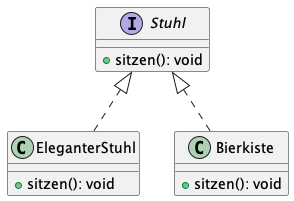
\includegraphics[width=0.4\textwidth]{fig/uml/stuhl-function.png}
  \caption{Funktionale Zerlegung mit Interface}
  \label{fig:stuhl-f}
\end{figure}

\begin{figure}[ht!]
  \centering
  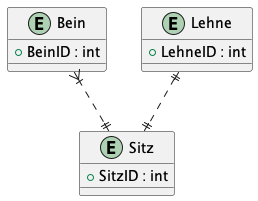
\includegraphics[width=0.4\textwidth]{fig/uml/stuhl-resourcen.png}
  \caption{Ressourcen-orientierte Zerlegung mit Relation}
  \label{fig:stuhl-r}
\end{figure}
Um den Unterschied der Ansätze nochmal zu verdeutlichen soll die Analogie der \enquote{Zerlegung eines Stuhls} als Sitzgelegenheit herangezogen werden. Wo bei der funktionalen Zerlegung die Suche nach einer Funktionen, wie das \enquote{Sitzen} im Vordergrund steht, und bei der ressourcenorientierten Zerlegung die Identifikation der einzlenen Ressourcen, wie (Stuhl-)Bein, Sitz(-fläche) oder (Rücken-)Lehne. Umgesetzt in ein Designentwurf für die funktionale Zerlegung ergibt sich beispielhaft in einer objektorientierten Sprache folgender der in dem Diagramm\ref{fig:stuhl-f} zu erkenne ist. 

In diesem Beispiel ist es wichtig zu erkennen, dass das Design mit der funktionalen Zerlegung auch seine Schwächen hat. Auch wenn eine korrekte Funktionssignatur bestimmt wurde, kann sich hinter dem Interface der realen Umsetzung dennoch eine nicht zu erwartende Umsetzung verbergen. In diesem  Beispiel wird beim Versuch sich zu setzen nicht nur ein eleganter Stuhl zu erwarten sein, sondern es kann auch eine Bierkiste die Sitzmöglichkeit repräsentieren. Diese Möglicheiten der Polymorphie eröffnet Chancen und Risiken.  
\\\\
Die ressourcenorientierte Zerlegung ist dahingehend intuitiver (siehe Abbildung \ref{fig:stuhl-r}, da ein System in seine einzelnen Ressourcen zerlegt wird, wobei diese eindeutig identifizierbar sein müssen. Auf diese Weise können diese Ressourcen als Entitäten Beziehungen zueinander aufbauen, welche wiederum mit weiteren Eigenschaften belegt werden können. In der korrekten Umsetzung ergibt sich so ein gutes Bild des Gesamtsystems. Die Gefahr besteht jedoch darin, dass die Ressourcen und deren Attribute nicht genau genug bestimmt werden oder die Beziehungen falsch beschrieben sind. In der hier benannten Analogie kann der Bausatz eines Stuhls auch auf eine Art und Weise beschrieben werden, dass die Lehne an den Beinen montiert ist und somit trotz identifizierter Ressourcen nicht den Dienst eines Stuhles, zumindest wie er erwartet wird, erfüllen kann.

Der geneigte Leser könnte als Übung hinterfragen, wie die Umsetzung eines Schachspiels in der funktionalen Zerlegung beschrieben werden könnte und wie dies in der ressourcenorientierten Zerlegung aussehen würde. So ergeben sich beispielhaft die Optionen, dass das Spielbrett sowohl in der objektorientierten Sprache durch eine Klasse mit Methoden ausgedrückt wird, die das Brett und die Spielregeln verwaltet, oder als Datenbankressource mit der gleichen Aufgabe.

Bei der Datenbank-Ressource werden die Spielzüge mit dem CRUD Interface realisiert. Spielregeln könnten durch Datenbank-Trigger erfasst werden. Ein Datenbank-Trigger ist ein spezielles Programm oder Skript, das  automatisch ausgeführt wird, wenn bestimmte Änderungen an einer Datenbanktabelle oder -sicht vorgenommen werden. Der Trigger wird auf eine bestimmte Aktion (z.B. INSERT, UPDATE oder DELETE) festgelegt und kann verwendet werden, um eine Reihe von Aufgaben oder Maßnahmen auszuführen, wenn diese Aktion auftritt.

\noindent\begin{minipage}{\textwidth}
\begin{lstlisting}[caption={Schachbrett - Objektorientiert},captionpos=b,label={lst:schachbrett-oo}]
public class ChessBoard {
    private Piece[][] board;

    public ChessBoard() {
        this.board = new Piece[8][8];
        // Initialize the board with the starting positions of pieces
        // e.g. add new Piece(PieceType.ROOK, Color.WHITE) to board[0][0] for the white rook in the top-left corner.
    }

    public Piece getPiece(int row, int col) {
        return board[row][col];
    }

    public void setPiece(int row, int col, Piece piece) {
        board[row][col] = piece;
    }

    // Other methods for checking if a move is valid, getting a list of possible moves, etc.
}
\end{lstlisting}
\end{minipage}

Die Wahl der richtigen Methode hängt von verschiedenen Faktoren ab, wie z.B. der Komplexität des Systems, der Art der Aufgaben, die ausgeführt werden müssen, und den verfügbaren Ressourcen.

Für die Zerlegung in einem verteilten System hat bereits die Auswahl der grundlegenden Strategie der Zerlegung einen hohen Einfluss. Die Schnittstellen der Systeme ändern sich dadurch und damit auch die notwendige Kommunikation und die Datenrepräsentation in den Systemen.\footnote{Eine weitere Art der Diskussion: \url{https://medium.com/double-pointer/system-design-interview-a-two-player-online-chess-game-4a150ad8ea78} }

\noindent\begin{minipage}{\textwidth}
\begin{lstlisting}[caption={Schachbrett - Datenbank},captionpos=b,label={lst:schachbrett-datenbank}]

CREATE TABLE ChessBoard (
    id INT PRIMARY KEY,
    row INT,
    col INT,
    pieceType VARCHAR(10),
    pieceColor VARCHAR(5)
);
\end{lstlisting}
\end{minipage}


\subsubsection{Datenseparation}

Die Datenseparation in verteilten Systemen bezieht sich auf den Prozess, bei dem Daten auf mehrere Knoten in einem Netzwerk verteilt werden, um die Leistung, Skalierbarkeit und Zuverlässigkeit des Systems zu verbessern. Dies wird typischerweise durch die Aufteilung von Daten in kleine Teile und deren Verteilung auf verschiedene Knoten oder Server im Netzwerk erreicht.
Es gibt verschiedene Möglichkeiten, Daten in verteilten Systemen zu separieren, einschließlich:
\begin{itemize}
\item \textbf{Horizontale Partitionierung}\index{Partitionierung}\index{horizontal}: Hierbei wird eine Tabelle in mehrere kleinere Tabellen aufgeteilt und jede Teilung wird auf einem separaten Server gespeichert. Zum Beispiel könnte man Kundeninformationen basierend auf Regionen oder Alphabeten auf verschiedene Server verteilen.

Ein Beispiel für ein Unternehmen, das Horizontale Partitionierung einsetzt, ist Facebook. Facebook speichert seine Daten in einer horizontal partitionierten Datenbank, bei der jede Tabelle in mehrere Teilbereiche aufgeteilt wird, wobei jeder Teilbereich nur bestimmte Zeilen enthält. Dies ermöglicht es Facebook, die Last auf mehrere Datenbankserver zu verteilen und eine bessere Skalierbarkeit zu erreichen. Wenn ein Benutzer beispielsweise eine Suche durchführt, kann Facebook nur die benötigten Zeilen abfragen und somit eine schnellere Antwortzeit erzielen.
\item \textbf{Vertikale Partitionierung}\index{Partitionierung}\index{vertikal}: Hierbei werden bestimmte Spalten einer Tabelle auf verschiedene Server verteilt. Zum Beispiel könnten personenbezogene Daten (Name, Geburtsdatum, Adresse usw.) auf einem Server gespeichert werden, während andere Daten wie Kontaktinformationen auf einem anderen Server gespeichert werden.

Ein Beispiel für eine Anwendung, die Vertikale Partitionierung einsetzt, ist die Online-Shop-Plattform Amazon. Amazon speichert seine Daten in einer vertikal partitionierten Datenbank, bei der jede Tabelle in mehrere Teilbereiche aufgeteilt wird, wobei jeder Teilbereich nur bestimmte Spalten enthält. Wenn ein Benutzer beispielsweise eine Suche nach einem bestimmten Produkt durchführt, kann Amazon nur die benötigten Spalten abfragen und somit eine schnellere Antwortzeit erzielen.

Ein weiteres Beispiel ist LinkedIn, die auch Vertikale Partitionierung nutzen, um ihre Datenbank effizienter zu gestalten. LinkedIn speichert ihre Nutzerdaten in verschiedenen Datenbanken, die jeweils auf bestimmte Anwendungen und Funktionen zugeschnitten sind. Dadurch können sie die Ladezeiten reduzieren und eine bessere Skalierbarkeit erreichen.
\item \textbf{Sharding}\index{Sharding}: Hierbei wird die Datenbank in kleine, unabhängige Teile aufgeteilt, die auf verschiedenen Servern gespeichert werden. Dies ermöglicht eine horizontale Skalierung und verbessert die Leistung des Systems. Sharding ist eine Art der horizontalen Partitionierung, die Daten auf der Grundlage eines Sharding-Schlüssels aufteilt.

Slack ist ein Beispiel für eine Anwendung, die eine Form des Sharding verwendet, um ihre Datenbankleistung zu skalieren. Sharding ist eine Technik, bei der eine Datenbank in mehrere Teilbereiche aufgeteilt wird, die als \enquote{Shards} bezeichnet werden. Jeder Shard enthält einen Teil der Daten, so dass die Datenbank effizienter und schneller durchsucht werden kann.

In Slack wird Sharding verwendet, um die Benutzerdaten zu partitionieren. Das bedeutet, dass die Daten der Benutzer in mehrere Shards aufgeteilt werden, um die Last auf mehrere Datenbankserver zu verteilen. Jeder Shard ist dabei in der Lage, seine eigene Last zu verarbeiten und kann unabhängig von den anderen Shards skaliert werden. Dadurch kann Slack eine höhere Skalierbarkeit und eine bessere Leistung erzielen.
\item Daten-\textbf{Replikation}: Hierbei werden Daten auf mehreren Knoten im Netzwerk gespeichert, um Redundanz und Fehlertoleranz zu gewährleisten. Wenn ein Knoten ausfällt, kann ein anderer Knoten die Arbeit übernehmen und sicherstellen, dass das System weiterhin funktioniert.
\end{itemize}
Die Datenseparation in verteilten Systemen ist ein wichtiger Aspekt für die Skalierung und die Verfügbarkeit von Anwendungen. Durch die Verteilung von Daten auf mehrere Knoten im Netzwerk kann das System schnell auf Anforderungen reagieren und bietet eine hohe Verfügbarkeit, selbst wenn einzelne Knoten ausfallen.

\subsubsection{Schnittstellen zwischen den Entitäten}

Verteilte Systeme bestehen aus mehreren eigenständigen \enquote{nodes}, die über ein Netzwerk miteinander verbunden sind und gemeinsam arbeiten. Jede node repräsentiert eine Funktion oder eine Ressource, bzw. die Orchestrierung im funktionalen bzw. ressource-orientierten Ansatz. Unabhängig der Zerlegungsmethode müssen diese nodes miteinander kommunizieren, um Daten auszutauschen und ihre Arbeit zu koordinieren. Hier sind einige Gründe, warum verteilte Systeme Kommunikation benötigen:

\begin{itemize}
\item Datenaustausch: In verteilten Systemen müssen Daten zwischen verschiedenen Computern ausgetauscht werden, um eine gemeinsame Aufgabe zu erfüllen. Beispielsweise müssen Datenbanken in verschiedenen Computern synchronisiert werden, damit jeder Computer auf die aktuellste Version der Daten zugreifen kann.
\item Ressourcenmanagement: In verteilten Systemen können Ressourcen wie Speicher, Prozessoren und Netzwerkbandbreite auf verschiedene Computer verteilt werden. Um diese Ressourcen effektiv zu nutzen, müssen die Computer miteinander kommunizieren und Ressourcenanforderungen und -freigaben koordinieren.
\item Koordination: In verteilten Systemen müssen die Computer miteinander kommunizieren, um Aufgaben zu koordinieren. Beispielsweise können sie Nachrichten austauschen, um sicherzustellen, dass jeder Computer über den Fortschritt der Aufgabe informiert ist und seinen Teil der Arbeit erledigt.
\item Fehlererkennung und -behebung: In verteilten Systemen kann ein Computer ausfallen oder fehlerhaft arbeiten. Die verbleibenden Computer müssen miteinander kommunizieren, um den Fehler zu erkennen und die Arbeit neu zu verteilen oder den fehlerhaften Computer auszuschließen.
\item Skalierung: In verteilten Systemen kann die Anzahl der Computer erhöht werden, um die Leistung zu verbessern oder um mit einer höheren Last umzugehen. Um diese Skalierbarkeit zu erreichen, müssen die Computer miteinander kommunizieren und ihre Arbeit effektiv aufteilen.
\end{itemize}    

\textbf{Kommunikation ist in verteilten Systemen unerlässlich}, somit muss diskutiert werden, welche Art der Kommunikation Unterstützung findet. Zunächst müssen aber die Freiheitsgrade identifiziert werden. 
Eine wesentliche Unterscheidung ist synchron und asynchron. Dies bezieht sich auf die Art und Weise, wie Informationen zwischen Systemen oder Komponenten über ihre Schnittstellen (Interfaces) ausgetauscht werden. Hier sind die Unterschiede zwischen synchrone und asynchrone Kommunikation:

\begin{itemize} 
\item Synchrone\index{synchrone} Kommunikation bedeutet, dass die Kommunikation in (beinah) Echtzeit stattfindet, d.h. der Sender wartet auf eine Antwort des Empfängers, bevor er mit der nächsten Aktion fortfährt. Beispielsweise kann eine Anwendung eine Anforderung an eine Datenbank senden und auf die Antwort der Datenbank warten, bevor sie mit der Verarbeitung der nächsten Anforderung fortfährt. Bei synchroner Kommunikation kann das System oder die Anwendung nur dann fortfahren, wenn die Antwort vollständig ist.
\item Asynchrone\index{asynchrone} Kommunikation hingegen bedeutet, dass die Kommunikation asynchron oder zeitversetzt erfolgt, d.h. der Sender sendet eine Nachricht an den Empfänger, ohne auf eine sofortige Antwort zu warten. Der Empfänger verarbeitet die Nachricht dann und sendet eine Antwort zurück, wenn er bereit ist. Beispielsweise kann eine Anwendung eine Anforderung an einen Server senden und ohne auf eine Antwort zu warten, mit der Verarbeitung der nächsten Anforderung fortfahren. Die Antwort des Servers wird später empfangen, wenn sie verfügbar ist.
\end{itemize}  
Synchrone Kommunikation ist einfach zu implementieren und zu kontrollieren, da der Sender auf eine Antwort des Empfängers wartet, bevor er fortfährt. Es ist jedoch langsam, da der Sender auf die Antwort des Empfängers warten muss, bevor er weitere Aktionen ausführen kann.

Asynchrone Kommunikation hingegen ist schneller, da der Sender die nächste Aktion ausführen kann, ohne auf die Antwort des Empfängers zu warten. Es ist jedoch schwieriger zu implementieren und zu kontrollieren, da der Sender und Empfänger möglicherweise nicht synchronisiert sind und es zu Datenverlust oder Fehlern kommen kann. \textbf{Bereits zu diesem Zeitpunkt sollte festgestellt werden, das ein Design mit asynchronen Aufrufen dennoch in Verteilten Systemen vorzuziehen ist}.
\\\\
Eine weitere Unterscheidung in der Kommunikation ist persistent\index{persistent} und transient\index{transient}. Persistente und transiente Kommunikation beziehen sich auf die Art und Weise, wie Daten in einem verteilten System übertragen werden und ob die Daten dauerhaft oder vorübergehend gespeichert werden.

Persistente Kommunikation bedeutet, dass die Daten, die zwischen den Systemen übertragen werden, dauerhaft gespeichert werden. Das bedeutet, dass die Daten im besten Fall auch nach einem Systemausfall oder einem Neustart des Systems noch verfügbar sind. Bei der persistenten Kommunikation wird die Datenübertragung oft über Protokolle wie das Transmission Control Protocol (TCP) abgewickelt, die sicherstellen, dass die Daten vollständig und fehlerfrei übertragen werden.

Transiente Kommunikation hingegen bedeutet, dass die Daten, die zwischen den Systemen uni- oder bidirektional übertragen werden, vorübergehend und nicht dauerhaft gespeichert werden. Das bedeutet, dass die Daten nach einem Systemausfall oder einem Neustart des Systems nicht mehr verfügbar sind. Transiente Kommunikation wird oft über Protokolle wie das User Datagram Protocol (UDP) abgewickelt, die schnell und effizient sind, aber keine Garantie dafür bieten, dass die Daten vollständig oder fehlerfrei übertragen werden.

Ein Beispiel für persistente Kommunikation ist die Übertragung von Daten zwischen einem Webserver und einer Datenbank. Die Daten, die von der Website an den Webserver gesendet werden, werden dauerhaft in der Datenbank gespeichert, damit sie jederzeit abgerufen werden können. Ein Beispiel für transiente Kommunikation ist das Streaming von Audio oder Video in Echtzeit, bei dem die Daten nur während des Streams verfügbar sind und nicht gespeichert werden müssen.
\\\\
Signal, Event und Nachricht sind drei Begriffe, die oft in der Informatik im Kontext der Kommunikation verwendet werden und leicht verwechselt werden können. Hier sind ihre Unterschiede:

\begin{itemize}  
\item (Call-)\textbf{Event}\index{Event}:
Ein Event ist ein Ereignis, das in einer Anwendung oder einem System auftritt und von einem Benutzer, einem anderen Prozess oder einer anderen Anwendung ausgelöst werden kann. Events können zum Beispiel ein Mausklick, ein Tastendruck, ein Datenbankupdate oder ein Systemalarm sein. Anwendungen können auf diese Ereignisse reagieren, indem sie bestimmte Aktionen ausführen.
\begin{figure}[!h]
  \centering
  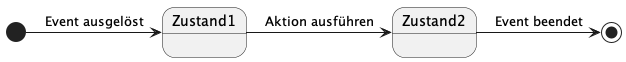
\includegraphics[width=0.95\textwidth]{fig/uml/simple-event.png}
  \caption{Einfaches Event}
  \label{fig:simple-event}
\end{figure}
Während ein Signal ein asynchrones Ereignis ist, ist ein (Call) Event im Allgemeinen synchron. Das bedeutet, dass wenn ein Objekt eine Operation auf einem anderen Objekt aufruft, die Kontrolle vom Sender an den Empfänger übergeben wird, bis die Operation abgeschlossen ist, woraufhin die Kontrolle zum Sender zurückkehrt. 

\item \textbf{Signal}\index{Signal}:
Ein Signal ist ein Ereignis, das von einem Betriebssystem oder einer Anwendung an eine andere Anwendung oder einen Prozess gesendet wird, um eine bestimmte Aktion auszulösen. Signale können zum Beispiel verwendet werden, um einen Prozess zu beenden, ein bestimmtes Verhalten auszulösen oder auf eine bestimmte Situation zu reagieren.
\begin{figure}[!h]
  \centering
  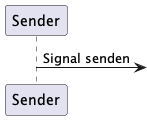
\includegraphics[width=0.25\textwidth]{fig/uml/simple-signal.png}
  \caption{Einfaches Signal}
  \label{fig:simple-signal}
\end{figure}
In der Modellierung der Architektur hat dies eine besondere Bedeutung, da ein Signal ein Objekt repräsentiert, das von einem Objekt asynchron ausgelöst wird und dann von einem anderen empfangen wird. Ein Beispiel hierfür sind Fehlerbehandlungen (Exceptions). Dem Signal ist keine Operation zugeordnet. Die Modellierung einer Klasse oder der Schnittstelle ist ein wichtiger Teil der Spezifikation. So kann definiert werden welches Signal durch die Operationen hinter einem Interface gesendet werden können.

\item \textbf{Nachricht}\index{Nachricht}:
Eine Nachricht ist eine Mitteilung, die von einer Anwendung, einem Prozess oder einem System an eine andere Anwendung, einen Prozess oder ein System gesendet wird. Nachrichten können zum Beispiel verwendet werden, um Daten zwischen verschiedenen Anwendungen oder Systemen auszutauschen, um einen bestimmten Prozess zu starten oder um Informationen über den Status eines Prozesses zu übermitteln. 
\begin{figure}[!h]
    \centering
    \begin{subfigure}[b]{0.45\textwidth}
      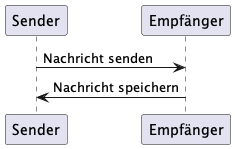
\includegraphics[width=0.8\textwidth]{fig/uml/async-message.png}
      \caption{Asynchrone Nachricht}
      \label{fig:async-msg}
    \end{subfigure}
    \hfill
    \begin{subfigure}[b]{0.45\textwidth}
        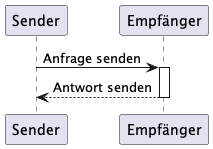
\includegraphics[width=0.75\textwidth]{fig/uml/sync-message.png}
        \caption{Synchrone Nachricht}
        \label{fig:sync-msg}
    \end{subfigure}
    \caption{}
    \label{fig:gesamt}
\end{figure}
\end{itemize}  
Bei Nachrichten gibt es normalerweise einen expliziten Sender und Empfänger, die durch Adressen oder IDs identifiziert werden. Der Sender sendet eine Nachricht an einen bestimmten Empfänger, der die Nachricht empfängt und darauf reagiert.

Dies soll auch nochmals mit den Events verglichen werden. Bei Events hingegen gibt es normalerweise keinen expliziten Sender oder Empfänger. Ein Event tritt auf, und Anwendungen oder Prozesse, die auf dieses Event hören, können darauf reagieren. 
\\\\
Weiter kann das versenden von Nachrichten sowohl synchron oder asynchron aufgefasst werden. Bei einem synchronen Aufruf exisitert eine Sende- und eine Empfangsnachricht. Bei einem asynchronen Aufruf, exisitert tyischerweise nur eine Sendenachricht.
\\\\
Signale und Events sind Ereignisse, die in einem System auftreten, während eine Nachricht eine Mitteilung ist, die zwischen verschiedenen Systemen ausgetauscht wird. Signale werden normalerweise zwischen verschiedenen Prozessen oder Anwendungen im selben System verwendet, während Events normalerweise innerhalb einer Anwendung auftreten. Nachrichten werden normalerweise zwischen verschiedenen Anwendungen oder Systemen ausgetauscht.

Events, Signale und Nachrichten bilden die Grundlage für weiterführende Konzepte in der Schnittstellenkonzeptionierung von verteilten Systmen:
\begin{itemize}  
\item \textbf{Remote Procedure Call} (RPC): Hierbei wird eine Funktion auf einem entfernten System aufgerufen, als ob sie lokal ausgeführt würde. Der Aufruf wird über das Netzwerk gesendet und das entfernte System führt die Funktion aus und gibt das Ergebnis zurück.
\item \textbf{Shared Memory}: Hierbei wird ein gemeinsamer Speicherbereich zwischen verschiedenen Knoten im System verwendet, auf den alle Knoten zugreifen können. Dadurch können Daten schnell und effizient zwischen Knoten geteilt werden.
\item \textbf{Datenbank-Replikation}: Hierbei werden Datenbanken auf verschiedenen Knoten im System repliziert, um die Verfügbarkeit und Skalierbarkeit zu verbessern. Änderungen an einer Datenbank werden automatisch an andere replizierte Datenbanken weitergeleitet, um sicherzustellen, dass alle Knoten im System auf dieselben Daten zugreifen können.
\item \textbf{Stream Processing}: Hierbei werden Daten in Echtzeit von verschiedenen Knoten im System gestreamt und verarbeitet, um Echtzeit-Analysen und -Verarbeitung zu ermöglichen. Stream Processing wird oft in Anwendungen wie Finanzdienstleistungen, E-Commerce und Social-Media-Anwendungen eingesetzt.
\end{itemize}  
Diese Möglichkeiten sollen auch mehr im Detail im Kontext der Architekturparadigmen diskutiert werden.

\subsubsection{Kopplung}
Bevor sich den Architekturen zugewendet wird, soll noch einige weitere wichtige Begriffe im Design verteilter Systeme eingebracht werden: Ein wichtiger ist der Kopplungsbegriff. 

Der Kopplungsbegriff ist in verteilten Systemen von entscheidender Bedeutung, da er die Art und Weise beschreibt, wie verschiedene Anwendungen und Systeme in einem verteilten System miteinander interagieren und kommunizieren. Eine falsche Wahl der Kopplungsart kann zu schwerwiegenden Problemen führen, die die Interoperabilität und Integration von Anwendungen in einem verteilten System beeinträchtigen können.
\\\\
Die Wahl der richtigen Kopplungsart kann jedoch auch erhebliche Vorteile bieten. Eine direkte Kopplung kann zu einer höheren Leistung führen und eine bessere Integration von Anwendungen ermöglichen, während eine indirekte Kopplung die Skalierbarkeit und Zuverlässigkeit verbessern kann. Eine losgekoppelte Architektur kann die Flexibilität  und die Ausfallsicherheit erhöhen, während eine strukturelle Kopplung die Zusammenarbeit und Integration von Anwendungen erleichtern kann. Im Detail ist es nochmal in der Tabelle\ref{tab:kopplungsarten} nochmal diskutiert.
\\\\
\begin{table}[!h]
  \centering
  \caption{Kopplungsarten in verteilten Systemen}
  \label{tab:kopplungsarten}
  \begin{tabular}{|p{4cm}|p{7cm}|}
    \hline
    \textbf{Kopplungsart} & \textbf{Beschreibung} \\ \hline
    Direkte Kopplung & Die Anwendungen und Systeme in einem verteilten System sind direkt miteinander verbunden und kommunizieren direkt miteinander. \\ \hline
    Indirekte Kopplung & Die Anwendungen und Systeme in einem verteilten System kommunizieren über ein gemeinsames Mediator-System oder eine Middleware miteinander. \\ \hline
    Losgekoppelte Kopplung & Die Anwendungen und Systeme in einem verteilten System kommunizieren über Nachrichten, ohne sich direkt zu verbinden. \\ \hline
    Strukturelle Kopplung & Die Anwendungen und Systeme in einem verteilten System sind durch gemeinsame Datenstrukturen oder Datentypen verbunden. \\ \hline
  \end{tabular}
\end{table}
Eine direkte Kopplung tritt auf, wenn Anwendungen oder Systeme direkt miteinander verbunden sind und direkt miteinander kommunizieren. Beispielsweise können zwei Anwendungen über eine Netzwerkverbindung oder einen direkten Datenlink verbunden sein und direkt miteinander kommunizieren.
\\
Eine indirekte Kopplung tritt auf, wenn Anwendungen oder Systeme über ein gemeinsames Mediator-System oder eine Middleware miteinander kommunizieren. Das Mediator-System oder die Middleware stellt eine Abstraktionsschicht bereit, die die Interoperabilität und Integration von Anwendungen in einem verteilten System erleichtert.

Eine losgekoppelte Kopplung tritt auf, wenn Anwendungen oder Systeme über Nachrichten kommunizieren, ohne sich direkt zu verbinden. In diesem Fall sendet eine Anwendung eine Nachricht an eine Middleware oder einen Broker, der die Nachricht an die Empfängeranwendung weiterleitet.

Eine strukturelle Kopplung tritt auf, wenn Anwendungen oder Systeme durch gemeinsame Datenstrukturen oder Datentypen verbunden sind. Beispielsweise können Anwendungen über eine gemeinsame Datenbank oder eine gemeinsame Dateistruktur kommunizieren. Die Tabelle~\ref{tab:kopplungsarten} gibt nochmals einen Überblick mit den Definitionen. 

\subsubsection{Mechanismen und Policies}

Mechanismen\index{Mechanismen} sind die grundlegenden Bausteine oder Funktionen, die zur Implementierung von verteilten Systemen benötigt werden. Policies hingegen sind die Entscheidungsregeln oder Leitlinien, die bestimmen, wie die Mechanismen eingesetzt und betrieben werden.
\\\\
Beispiele von Mechanismen in verteilten Systemen:
\begin{itemize} 
\item Kommunikation: In verteilten Systemen müssen die Knoten miteinander kommunizieren, um Daten auszutauschen und zusammenzuarbeiten. Mechanismen wie Message Passing, Remote Procedure Calls (RPC) und Remote Method Invocation (RMI) ermöglichen diese Kommunikation.
\item Synchronisation: Da verteilte Systeme aus mehreren unabhängigen Knoten bestehen, ist es wichtig, ihre Aktionen und Ressourcenzugriffe zu synchronisieren. Mechanismen wie Locks, Semaphore, Monitore und Barrieren werden verwendet, um die Synchronisation zu erreichen.
\item Replikation: Die Replikation ist ein Mechanismus, bei dem Daten oder Dienste auf mehreren Knoten im verteilten System dupliziert werden, um die Verfügbarkeit, Fehlertoleranz und Leistung zu verbessern.
\item Konsistenz: Um die Datenintegrität in verteilten Systemen aufrechtzuerhalten, müssen Mechanismen zur Gewährleistung der Konsistenz der Daten eingesetzt werden. Beispiele sind sequentielle Konsistenz, kausale Konsistenz, eventual Konsistenz und ACID-Transaktionen.
\end{itemize} 
Beispiele von Policies\index{Policies} in verteilten Systemen:
\begin{itemize} 
\item Ressourcenallokation: In verteilten Systemen müssen Entscheidungen darüber getroffen werden, wie Ressourcen wie Rechenleistung, Speicherplatz und Bandbreite zugewiesen werden. Beispiele für Ressourcenallokations-Policies sind First-Come-First-Served (FCFS), Round Robin, Prioritätswarteschlangen und Fair-Share-Scheduling.
\item Fehlerbehandlung: Policies zur Fehlerbehandlung legen fest, wie verteilte Systeme auf Fehler wie Hardware- oder Softwareausfälle, Netzwerkstörungen oder Datenverlust reagieren. Beispiele für Fehlerbehandlungspolicies sind Retry, Timeout, Fallback auf Alternativen und Datenwiederherstellung.
\item Sicherheit: Sicherheits-Policies bestimmen, wie verteilte Systeme den Schutz von Daten, Diensten und Benutzern gewährleisten. Beispiele sind Authentifizierung, Autorisierung, Verschlüsselung und Auditing.
\item Lastverteilung: Lastverteilungspolicies legen fest, wie die Arbeitslast in verteilten Systemen auf die verschiedenen Knoten verteilt wird, um eine optimale Leistung und Ressourcenauslastung zu erreichen. Beispiele sind statische Lastverteilung, dynamische Lastverteilung und adaptives Load Balancing.
\end{itemize}     

Als Beispiel für die Ausprägung soll die Lastverteilung in einem verteilten System gewählt sein, welche genutzt wird um einen  Webserver-Cluster zu betreiben. In diesem Fall ist Lastverteilung zunächst ein Mechanismus, der die Arbeitslast über mehrere Server oder Knoten verteilt, um eine bessere Leistung, Verfügbarkeit und Skalierbarkeit zu erreichen. Um eine effektive Lastverteilung zu ermöglichen, kann ein Load Balancer eingesetzt werden. Der Load Balancer ist dafür verantwortlich, ankommende Anfragen an die verschiedenen Server im Cluster weiterzuleiten.
Zudem kann die Policy darin bestehen, zu entscheiden, wie die Lastverteilung durchgeführt werden soll. Es gibt verschiedene Policies, die angewendet werden können, wie z. B. Round Robin, Least Connections oder Weighted Round Robin.
\begin{itemize} 
\item Round Robin: Der Load Balancer verteilt die Anfragen gleichmäßig auf alle verfügbaren Server, indem er sie der Reihe nach an jeden Server sendet.
\item Least Connections: Der Load Balancer leitet Anfragen an den Server weiter, der derzeit die wenigsten aktiven Verbindungen hat.
\item Weighted Round Robin: Der Load Balancer verteilt die Anfragen basierend auf dem Gewicht jedes Servers, das normalerweise die Kapazität oder Leistungsfähigkeit des Servers widerspiegelt.
\end{itemize}  
In diesem Beispiel ist der Lastverteilungsmechanismus (Load Balancer) für die Verteilung der Arbeitslast auf die verschiedenen Server im Cluster verantwortlich, während die Lastverteilungspolicy die Methode bestimmt, nach der die Verteilung erfolgen soll (Round Robin, Least Connections oder Weighted Round Robin). Die Policy kann je nach den spezifischen Anforderungen und Zielen des verteilten Systems ausgewählt und angepasst werden, diese Auswahl für jeden Mechanismus anzubieten, kann die Komplexität der Gesamtanwendung aber auch extrem steigern, so das mit einem Mechanismus nicht selten auch direkt die Policy im Mechanismus festgeschrieben wird.  

Ein anderes Beispiel ist näher an der Programmierung. Ein Vergleich zwischen einer API, die die Methoden left, right, up und down verwendet (Variante I), und einer API, die die Methode move(direction) verwendet (Variante II). Variante I ist in der Regel einfacher und direkt, da jede Methode jeweils eine einzelne Bewegungsrichtung repräsentiert. Dies führt zu einer besseren Typsicherheit, da es unwahrscheinlicher ist, dass ungültige Richtungen verwendet werden. Der Nachteil dieser API besteht darin, dass sie aus vier separaten Methoden besteht, was den Code länger und weniger flexibel machen kann. Außerdem ist diese API weniger skalierbar, da für die Hinzufügung neuer Richtungen jeweils neue Methoden erstellt werden müssten.

Auf der anderen Seite erlaubt die API mit der move(direction) Methode mehr Flexibilität, da die gewünschte Richtung als Parameter übergeben wird. Dies erleichtert die Steuerung der Bewegung in verschiedenen Szenarien. Die Skalierbarkeit ist ebenfalls höher, da beim Hinzufügen neuer Richtungen einfach neue Richtungsparameter eingebracht werden können, ohne dass neue Methoden erstellt werden müssen. Da nur eine Methode vorhanden ist, ist der Code kürzer und einfacher zu warten. Der Nachteil dieser API besteht darin, dass sie eine geringere Typsicherheit aufweist, da die Richtung als Parameter übergeben wird und somit die Möglichkeit besteht, dass ungültige oder unerwartete Richtungen verwendet werden.

\subsubsection{Stateful und stateless}
In verteilten Systemen beziehen sich die Begriffe \enquote{stateful}\index{stateful} und \enquote{stateless}\index{stateless} auf die Art und Weise, wie Systemkomponenten den Zustand ihrer Interaktionen verwalten.
\\\\
\textbf{Stateful}:\\
Ein stateful System speichert Informationen über den aktuellen Zustand der Kommunikation zwischen den Komponenten. Das bedeutet, dass ein stateful Service oder eine stateful Anwendung auf vorherige Anfragen oder Interaktionen Bezug nimmt und auf der Grundlage dieser Informationen reagiert. Stateful Systeme sind oft komplexer, da sie den Zustand der Interaktionen aktiv verwalten und speichern müssen. Sie können jedoch auch leistungsfähiger sein, da sie auf der Grundlage früherer Interaktionen individuellere oder optimierte Antworten liefern können.
\\\\
\textbf{Stateless}:\\
Ein stateless System speichert keine Informationen über den aktuellen Zustand der Kommunikation zwischen den Komponenten. Jede Anfrage oder Interaktion wird isoliert betrachtet, ohne Bezug auf frühere Anfragen oder Interaktionen. Stateless Systeme sind in der Regel einfacher zu implementieren und zu skalieren, da sie keine kontinuierliche Zustandsverwaltung erfordern. Sie können jedoch weniger leistungsfähig sein, wenn sie auf Informationen aus früheren Interaktionen angewiesen sind, um effektiv zu funktionieren.
\\\\
In verteilten Systemen können Nachrichtenabhängigkeiten einen Einfluss auf die stateful- oder stateless-Eigenschaften eines Systems haben. Nachrichtenabhängigkeiten treten auf, wenn die Verarbeitung einer Nachricht von der Verarbeitung einer oder mehrerer vorheriger Nachrichten abhängig ist. In solchen Fällen ist es erforderlich, den Zustand der Kommunikation zu verfolgen, um sicherzustellen, dass die Nachrichten in der richtigen Reihenfolge verarbeitet werden und das System korrekt funktioniert.
\begin{itemize}  
\item \textbf{Stateful Systeme}: Nachrichtenabhängigkeiten sind in stateful Systemen von Natur aus einfacher zu handhaben, da diese Systeme bereits den Zustand der Interaktionen verwalten. In stateful Systemen kann die Verarbeitung einer Nachricht auf früheren Nachrichten aufbauen, und das System kann sicherstellen, dass Nachrichten in der richtigen Reihenfolge verarbeitet werden.
\item \textbf{Stateless Systeme}: In stateless Systemen ist die Handhabung von Nachrichtenabhängigkeiten schwieriger, da kein Zustand zwischen den Anfragen gespeichert wird. Um Nachrichtenabhängigkeiten in stateless Systemen zu bewältigen, können Techniken wie das Hinzufügen von Sequenznummern oder Zeitstempeln zu Nachrichten verwendet werden, um die korrekte Reihenfolge der Nachrichtenverarbeitung sicherzustellen. In einigen Fällen müssen stateless Systeme den Zustand extern speichern oder verwalten, um Nachrichtenabhängigkeiten effektiv zu behandeln.
\end{itemize}  

Als ein Beispiel für einen zustandsbehafteten Dienst soll der Dateisystemserver eingebracht werden, welcher zuch Zustandsvariant ist.  Ein Dateisystemserver, der seinen Zustand oder seine Zustandsmaschine anpasst, basierend auf den empfangenen Nachrichten, kann daher als zustandsbehaftet oder stateful bezeichnet werden. In einem zustandsbehafteten System speichert der Server Informationen über die Interaktionen mit Clients, wie zum Beispiel offene Dateien, Positionen innerhalb von Dateien oder Benutzerberechtigungen.
\\\\
Wenn der Dateisystemserver eine Anfrage empfängt, z. B. zum Öffnen einer Datei, zum Lesen oder Schreiben von Daten oder zum Ändern von Berechtigungen, aktualisiert er seine Zustandsmaschine entsprechend. Die serverseitige Zustandsmaschine kann Informationen darüber enthalten, welche Dateien gerade geöffnet sind, welche Operationen auf ihnen ausgeführt werden und welche Benutzer Zugriff auf sie haben.

Durch das Beibehalten eines Zustands kann der Dateisystemserver effizienter arbeiten, da er die Informationen über die aktuellen Interaktionen und Operationen speichert und darauf zugreifen kann, ohne sie jedes Mal neu abrufen oder berechnen zu müssen. Allerdings bringt diese zustandsbehaftete Architektur auch Herausforderungen in Bezug auf Skalierbarkeit, Fehlertoleranz und Ressourcenverwaltung mit sich.

Die Wahl zwischen stateful und stateless Architekturen von den Anforderungen des verteilten Systems ab. Stateless Systeme bieten Vorteile in Bezug auf Einfachheit und Skalierbarkeit, während stateful Systeme besser für Anwendungen geeignet sind, bei denen der Kontext früherer Interaktionen für die korrekte Bearbeitung notwendig sind. 

\subsubsection{Transaktion}
In verteilten Systemen ist eine Transaktion eine Sequenz von Operationen, die auf verteilten Ressourcen oder Daten ausgeführt werden, um eine bestimmte Aufgabe oder Funktion zu erfüllen. Transaktionen sind wichtig, um die Konsistenz und Integrität von Daten in verteilten Systemen zu gewährleisten, insbesondere bei gleichzeitigen Zugriffen und Änderungen durch verschiedene Benutzer oder Prozesse.

Transaktionen in verteilten Systemen sollten die ACID-Eigenschaften (Atomicity, Consistency, Isolation, Durability) erfüllen:
\begin{itemize}
\item Atomicity (Atomarität): Eine Transaktion besteht aus einer Reihe von Operationen. Entweder werden alle Operationen erfolgreich ausgeführt und die Transaktion ist abgeschlossen, oder bei einem Fehler werden alle Operationen rückgängig gemacht, als ob die Transaktion nie stattgefunden hätte.
\item Consistency (Konsistenz): Transaktionen stellen sicher, dass das verteilte System von einem konsistenten Zustand in einen anderen konsistenten Zustand übergeht, auch wenn Fehler oder gleichzeitige Zugriffe auftreten.
\item Isolation (Isolierung): Jede Transaktion wird so ausgeführt, als ob sie isoliert von anderen gleichzeitig laufenden Transaktionen wäre. Dies bedeutet, dass die Zwischenergebnisse einer Transaktion für andere Transaktionen nicht sichtbar sind, bis die Transaktion abgeschlossen ist.
\item Durability (Dauerhaftigkeit): Sobald eine Transaktion abgeschlossen ist, sind ihre Änderungen dauerhaft im System gespeichert, selbst im Falle von Systemausfällen oder Fehlern.
\end{itemize}
Beispiele für Transaktionen in verteilten Systemen:
\begin{itemize}
\item Bankwesen: In einem verteilten Banksystem können Transaktionen verwendet werden, um Geldtransfers zwischen Konten durchzuführen. Die Transaktion stellt sicher, dass das Geld vom Senderkonto abgezogen und dem Empfängerkonto hinzugefügt wird, wobei die Konsistenz der Kontostände gewährleistet ist.
\item E-Commerce: In einem verteilten E-Commerce-System können Transaktionen verwendet werden, um Bestellungen und Zahlungen zu verarbeiten. Die Transaktion kann die Aktualisierung des Lagerbestands, die Berechnung von Steuern und Versandkosten, die Reservierung von Artikeln und die Verarbeitung der Zahlung beinhalten.
\item Verteilte Datenbanken: Bei verteilten Datenbanken werden Transaktionen verwendet, um sicherzustellen, dass mehrere Operationen, wie das Hinzufügen, Aktualisieren oder Löschen von Datensätzen, konsistent und gleichzeitig durchgeführt werden, ohne dass Inkonsistenzen oder Datenverluste auftreten.
\end{itemize}
Allerdings erfordert die Implementierung von Transaktionen in verteilten Systemen auch zusätzliche Überlegungen hinsichtlich Leistung, Fehlertoleranz und Koordination zwischen den beteiligten Knoten.
\\\\
Verschachtelte Transaktionen sind eine Erweiterung des grundlegenden Transaktionskonzepts, bei dem Transaktionen innerhalb einer übergeordneten Transaktion ausgeführt werden können. Diese innere Transaktion wird als \enquote{Untertransaktion} oder \enquote{Nested Transaction} bezeichnet. Eine verschachtelte Transaktion erlaubt es, dass Untertransaktionen unabhängig voneinander abgeschlossen oder abgebrochen werden, ohne die übergeordnete Transaktion als Ganzes zu beeinflussen.

Verschachtelte Transaktionen bieten Vorteile in Bezug auf Modularität, Fehlerbehandlung und Leistung, insbesondere in verteilten Systemen und bei komplexen Abläufen. Sie ermöglichen es, Teile einer größeren Transaktion separat abzuschließen und bei Fehlern nur die betroffenen Teile zurückzurollen, anstatt die gesamte Transaktion rückgängig zu machen.
\\\\
Ein Transaktionsmanager, auch als Transaktionskoordinator oder Transaktionsmonitor bezeichnet, ist eine Komponente in einem verteilten System, die für das Management und die Koordination von Transaktionen verantwortlich ist. Der Transaktionsmanager hat folgende Hauptaufgaben:
\begin{itemize}
\item Koordination: Der Transaktionsmanager koordiniert die beteiligten Ressourcen und Knoten in einer verteilten Transaktion, um sicherzustellen, dass sie konsistent und korrekt ausgeführt wird.
\item Protokollierung und Wiederherstellung: Der Transaktionsmanager führt ein Transaktionsprotokoll, um Änderungen und Aktivitäten während der Transaktion aufzuzeichnen. Im Falle eines Fehlers oder Systemausfalls verwendet der Transaktionsmanager das Protokoll, um den Zustand der beteiligten Ressourcen wiederherzustellen und die Transaktion entweder abzuschließen oder zurückzurollen.
\item Isolierung und Synchronisation: Der Transaktionsmanager stellt sicher, dass Transaktionen isoliert voneinander ausgeführt werden, um die Konsistenz und Integrität der Daten zu gewährleisten. Er ist auch für die Synchronisation von Zugriffen und Aktualisierungen auf verteilte Ressourcen verantwortlich, um Deadlocks und Konflikte zu vermeiden.
\item Commit und Rollback: Der Transaktionsmanager ist verantwortlich für das endgültige Commit (Abschluss) oder Rollback (Rückgängigmachung) einer Transaktion. Bei erfolgreicher Ausführung aller Operationen wird die Transaktion abgeschlossen und die Änderungen dauerhaft gespeichert. Im Falle eines Fehlers oder einer nicht erfüllten Bedingung führt der Transaktionsmanager einen Rollback durch, um die betroffenen Ressourcen in ihren vorherigen Zustand zurückzusetzen.
\end{itemize}
Ein Transaktionsmanager spielt eine entscheidende Rolle bei der Sicherstellung der Konsistenz, Integrität und Fehlertoleranz in verteilten Systemen, die Transaktionen verwenden. Das Konzept ist auch größer als aus einfachen Beispielen hervorgeht, die Bedeutung wird erst in der Flexibilität  deutlich. Dennoch soll ein Beispiel versucht werden, wo drei unabhängige Dienste: Flug, Hotel und Mietwagen zu einem neuen, vorher nicht vorhandenen Dienst zusammengefügt wird. 

Zuerst beginnt der Transaktionsmanager eine neue Transaktion. In dieser Transaktion werden die erforderlichen Ressourcen von den drei Diensten reserviert: Flugbuchung, Hotelbuchung und Mietwagenbuchung. Anschließend prüft der Transaktionsmanager, ob alle erforderlichen Ressourcen erfolgreich reserviert wurden und ob die Verfügbarkeit für den gewünschten Zeitraum gegeben ist.

Wenn alle Reservierungen erfolgreich sind und die Verfügbarkeit für den gewünschten Zeitraum bestätigt wurde, führt der Transaktionsmanager die Transaktion aus und erstellt die Urlaubsreise. Dabei wird der Gesamtpreis für Flug, Hotel und Mietwagen berechnet und dem Kunden in Rechnung gestellt. Nach erfolgreicher Zahlung bestätigt der Transaktionsmanager die Buchungen für die einzelnen Dienste und speichert die Informationen für die Urlaubsreise im System.

Falls jedoch eine oder mehrere Reservierungen nicht erfolgreich sind oder die Verfügbarkeit für den gewünschten Zeitraum nicht gegeben ist, wird der Transaktionsmanager die Transaktion abbrechen. In diesem Fall werden alle bisher reservierten Ressourcen für Flug, Hotel und Mietwagen freigegeben und der Kunde wird darüber informiert, dass die Urlaubsreise nicht erstellt werden konnte.

Der Transaktionsmanager stellt sicher, dass entweder alle Dienste erfolgreich kombiniert und die Urlaubsreise erstellt wird, oder keine der Reservierungen erfolgt und die Ressourcen wieder freigegeben werden. Dadurch wird ein konsistenter Zustand in den verteilten Systemen gewährleistet und es wird verhindert, dass teilweise reservierte oder unvollständige Urlaubsreisen entstehen.
\subsubsection{Message Passing}
Message Passing ist ein Kommunikationsparadigma in verteilten Systemen, bei dem Prozesse oder Komponenten Nachrichten austauschen, um Daten zu übertragen oder Aufgaben zu koordinieren. Es ist ein grundlegendes Konzept in der Kommunikation zwischen verteilten Einheiten und bildet die Basis für viele verteilte Systemarchitekturen, aber auch darüber hinaus.
Message Passing ist ein Konzept für die Nebenläufigkeits-Programmierung (Concurrent programming), der parallelen Programmierung (Parallel programming), der objektorientierten Programmierung und der Interprozesskommunikation.

Im Message Passing werden Nachrichten, die Daten oder Anweisungen enthalten, zwischen Prozessen oder Komponenten übermittelt. Die Kommunikation erfolgt in der Regel asynchron, d. h., der sendende Prozess wartet nicht darauf, dass der empfangende Prozess die Nachricht empfängt oder verarbeitet. Dies ermöglicht eine lose Kopplung der Komponenten und erleichtert die Skalierung und Fehlertoleranz des Systems. Die Eigenschaften von Message Passing können wie folgt zusammengefasst werden:
\begin{itemize}
\item Asynchrone Kommunikation: Die Kommunikation ist in der Regel asynchron, wodurch Prozesse unabhängig voneinander weiterarbeiten können, ohne auf Antworten warten zu müssen.
\item Lose Kopplung: Die Kommunikation zwischen Prozessen ist indirekt und erfordert keine direkte Kenntnis der beteiligten Prozesse, was zu einer losen Kopplung der Komponenten führt.
\item Skalierbarkeit: Message Passing eignet sich gut für verteilte Systeme mit einer großen Anzahl von Prozessen oder Komponenten, da es einfacher ist, zusätzliche Knoten hinzuzufügen und die Kommunikation zwischen ihnen zu verwalten.
\end{itemize}
Beispiele für Message Passing in verteilten Systemen:
\begin{itemize}
\item Message Queues: Message Queues sind Datenstrukturen, die zum Speichern und Übertragen von Nachrichten zwischen verteilten Prozessen verwendet werden. Beispiele für Message Queue-Systeme sind RabbitMQ, Apache Kafka und Amazon SQS. Sie ermöglichen die asynchrone Kommunikation und die Entkopplung von sendenden und empfangenden Prozessen.

\item Message Passing Interface (MPI): MPI ist ein Standard für die Kommunikation zwischen Prozessen in verteilten Systemen, insbesondere in High-Performance-Computing-Umgebungen. MPI stellt Funktionen zum Senden und Empfangen von Nachrichten, Synchronisation von Prozessen und Gruppenkommunikation bereit.

\item Publish-Subscribe-Systeme: In diesem Modell senden Publisher Nachrichten an Topics, während Subscriber Nachrichten von den Topics empfangen, die sie abonniert haben. Beispiele für Publish-Subscribe-Systeme sind Google Cloud Pub/Sub, Apache Pulsar und MQTT. Dieses Modell ist ereignisgetrieben und ermöglicht eine lose Kopplung der beteiligten Prozesse.
\end{itemize}
Message Passing ist ein grundlegendes Konzept in verteilten Systemen und ermöglicht die Kommunikation und Koordination zwischen Prozessen oder Komponenten in einer skalierbaren und fehlertoleranten Weise.

Das Actor-Modell ist ein Konzept für das Design von verteilten Systemen, das auf der Idee von unabhängigen Entitäten basiert, die als \enquote{Actoren} bezeichnet werden. Actoren sind grundlegende Recheneinheiten, die einen Zustand besitzen und in der Lage sind, Nachrichten zu empfangen und zu verarbeiten. Es setzt auf das Konzept von Message Passing auf. In diesem Modell kommunizieren Actoren ausschließlich über asynchrone Nachrichtenübermittlung, wodurch sie lose gekoppelt und hochgradig parallelisierbar sind. Die Hauptprinzipien des Actor-Modells sind:
\begin{itemize}
\item Isolation: Jeder Actor verwaltet seinen eigenen Zustand und verarbeitet Nachrichten unabhängig von anderen Actoren. Diese Isolation ermöglicht eine hohe Fehlertoleranz und erleichtert die Wartung und Skalierung des Systems.

\item Nachrichtenbasierte Kommunikation: Actoren kommunizieren über asynchrone Nachrichten. Nachrichten werden in Mailboxen abgelegt und von Actoren verarbeitet, wenn sie dazu bereit sind. Dieser Ansatz reduziert die Notwendigkeit von Locking- und Synchronisierungsmechanismen und ermöglicht eine hohe Parallelität.

\item Lokalitätstransparenz: Actoren können unabhängig von ihrer physischen Lage im verteilten System agieren. Die Kommunikation zwischen Actoren ist transparent und unabhängig von der Verteilung der Actoren im System.

\item Fehlertoleranz: Durch die Isolation der Actoren und ihre unabhängige Verarbeitung von Nachrichten können Fehler auf einzelne Actoren beschränkt bleiben, ohne das gesamte System zu beeinträchtigen. Das Actor-Modell unterstützt auch Supervision, bei der ein Actor die Verantwortung für das Überwachen und Wiederherstellen anderer Actoren bei Fehlern übernimmt.
\end{itemize}


\subsubsection{Idempotent}

Idempotenz\index{idempotenz} ist ein wichtiger Begriff in der Informatik und bezieht sich auf die Eigenschaft von Operationen, die wiederholt ausgeführt werden können, ohne dass sich das Ergebnis nach der ersten Anwendung ändert. Eine idempotente Operation ist eine, bei der das mehrmalige Anwenden auf dasselbe Eingabematerial das gleiche Ergebnis liefert, als ob sie nur einmal ausgeführt worden wäre.

Die Bedeutung von Idempotenz für verteilte Systeme liegt in ihrer Fähigkeit, die Robustheit und Zuverlässigkeit zu verbessern, insbesondere in Situationen, in denen Netzwerkfehler, Duplizierung von Nachrichten oder unvorhersehbare Verzögerungen auftreten können. In verteilten Systemen kann es schwierig sein, den genauen Zustand des Systems zu bestimmen, und es kann nicht garantiert werden, dass Nachrichten oder Anforderungen immer in der richtigen Reihenfolge oder genau einmal ankommen.

Indem idempotente Operationen in verteilten Systemen verwendet werden, können einige der Herausforderungen im Zusammenhang mit Fehlern und Unvorhersehbarkeiten bewältigt werden:
\begin{itemize}
\item Wiederholung von Anfragen: Wenn ein Client in einem verteilten System keine Antwort von einem Server erhält, kann es schwierig sein, festzustellen, ob die Anfrage verloren gegangen ist oder ob der Server die Anfrage einfach noch nicht verarbeitet hat. In solchen Fällen kann die Wiederholung einer idempotenten Anfrage ohne negative Auswirkungen erfolgen, da mehrmaliges Senden derselben Anfrage dasselbe Ergebnis wie das einmalige Senden liefert.
\item Fehlertoleranz: Idempotente Operationen können dazu beitragen, die Fehlertoleranz von verteilten Systemen zu erhöhen, indem sie die Auswirkungen von Nachrichtenduplikationen oder Netzwerkfehlern minimieren. Da idempotente Operationen dieselben Ergebnisse liefern, unabhängig davon, wie oft sie angewendet werden, können sie dazu beitragen, den Systemzustand trotz solcher Fehler konsistent zu halten.
\item Vereinfachung der Systementwicklung: Idempotenz kann dazu beitragen, die Komplexität von verteilten Systemen zu verringern, indem sie die Notwendigkeit von komplizierten Mechanismen zur Handhabung von Zustandsänderungen oder Fehlerbehebungen verringert. Da idempotente Operationen immer dieselben Ergebnisse liefern, unabhängig von ihrer Anwendungsreihenfolge, können Entwickler weniger Zeit damit verbringen, solche Mechanismen zu entwickeln, und sich stattdessen auf die Implementierung der Kernfunktionalität des Systems konzentrieren.
\end{itemize}

Ein Beispiel für die Verwendung von Idempotenz in verteilten Systemen ist das PUT-HTTP-Verb in HTTP-APIs. Das PUT-Verb wird verwendet, um eine Ressource mit einer bestimmten ID zu aktualisieren oder zu ersetzen. Wenn eine PUT-Anfrage mehrmals gesendet wird, bleibt das Ergebnis gleich, als ob die Anfrage nur einmal gesendet wurde. 


\subsubsection{Distributed Hash Table, DHT}

Distributed Hash Tables (DHTs\index{DHT}) sind ein Schlüssel-Wert-Speichersystem, das in verteilten Systemen eingesetzt wird. Sie bieten eine effiziente und dezentrale Möglichkeit, Schlüssel-Wert-Paare in einem Peer-to-Peer-Netzwerk zu speichern und abzurufen. In DHTs sind die Knoten des Netzwerks gleichberechtigt und es gibt keine zentrale Instanz, die die Speicherung und den Zugriff auf die Daten kontrolliert.

Die mathematische Grundlage von DHTs ist der konsistente Hashing-Algorithmus, der wie folgt dargestellt werden kann:

\begin{itemize}
\item Gegeben sei ein Schlüsselraum von $0$ bis $2^m - 1$, wobei $m$ die Anzahl der Bits ist, die zur Darstellung der Schlüssel verwendet werden.
\item Jeder Knoten und jeder Schlüssel im DHT wird durch eine eindeutige ID im Schlüsselraum repräsentiert. Die IDs können durch Hash-Funktionen wie z.B. SHA-1 erzeugt werden.
\item Die Knoten sind in einem logischen Ring angeordnet, basierend auf ihren IDs, der als "Ringraum" bezeichnet wird. Die Position eines Knotens im Ringraum wird durch seine ID bestimmt.
\item Um einen Wert für einen bestimmten Schlüssel zu speichern oder abzurufen, wird der Schlüssel zunächst durch dieselbe Hash-Funktion gehasht, die für die Erzeugung der Knoten-IDs verwendet wurde.
\item Der gehashte Schlüssel wird dann im Ringraum lokalisiert, und der zuständige Knoten für diesen Schlüssel ist derjenige, dessen ID gleich oder unmittelbar nach der gehashten Schlüssel-ID liegt. Dieser Knoten wird als \enquote{Verantwortlicher} für den Schlüssel bezeichnet.
\item Jeder Knoten speichert Informationen über eine kleine Anzahl anderer Knoten im Netzwerk, die als \enquote{Nachbarn} bezeichnet werden. Diese Nachbarn dienen zur Weiterleitung von Anfragen für Schlüssel, für die der aktuelle Knoten nicht verantwortlich ist.
\item Bei Änderungen im Netzwerk, wie zum Beispiel beim Hinzufügen oder Entfernen von Knoten, werden die Schlüssel-Wert-Paare entsprechend neu verteilt, um die Belastung gleichmäßig auf alle Knoten im Netzwerk zu verteilen.
\end{itemize}

%Termin-3 - vs-slides-chapter02-1
 
\subsection{Architekturparadigmen}

In den Verteilten Systemen gibt es verschiedene Architekturparadigmen, die beschreiben, wie Software- oder Computersysteme strukturiert und organisiert werden können. Zunächst soll ein Überblick gegeben werden, bevor die Ansätze genauer disktuiert werden. Die wichtigsten Architekturparadigmen für diese Ausarbeitung sind:
\begin{itemize}  
\item Schichtenarchitektur (Layered Architecture): Hierbei wird das System in mehrere Schichten unterteilt, wobei jede Schicht eine bestimmte Funktion erfüllt und auf der darunter liegenden Schicht aufbaut. Ein Beispiel ist die dreischichtige Architektur, die aus einer Präsentationsschicht, einer Anwendungsschicht und einer Datenspeicherschicht besteht.

\item Client-Server-Architektur: Hierbei wird das System in einen Client und einen Server unterteilt, wobei der Client Anfragen an den Server sendet und dieser daraufhin Antworten liefert. Diese Architektur eignet sich gut für Anwendungen, bei denen der Client nur eine begrenzte Anzahl von Funktionen benötigt, während der Server die komplexen Berechnungen durchführt.

\item Service-Orientierte Architektur (SOA): Hierbei wird das System in Services unterteilt, die unabhängig voneinander entwickelt und bereitgestellt werden können. Diese Architektur ermöglicht die flexible Integration von Services, um komplexe Anwendungen zu erstellen.

\item Ereignisgesteuerte Architektur (Event-Driven Architecture): Hierbei reagiert das System auf Ereignisse, indem es entsprechende Aktionen ausführt. Diese Architektur wird oft in Systemen verwendet, die auf Echtzeitereignisse reagieren müssen, wie z.B. in der Finanzindustrie oder in der Telekommunikation.

\item Microservices-Architektur: Hierbei wird das System in kleine, unabhängige Services unterteilt, die jeweils eine spezifische Funktion erfüllen. Diese Architektur ermöglicht eine bessere Skalierbarkeit und Flexibilität, da jeder Service unabhängig voneinander entwickelt, getestet und bereitgestellt werden kann.

\item Peer-to-Peer-Architektur (P2P): Hierbei wird das System in ein Netzwerk von gleichwertigen Teilnehmern unterteilt, die direkt miteinander kommunizieren können, ohne auf einen zentralen Server angewiesen zu sein. Diese Architektur wird oft in Filesharing- und Kryptowährungsanwendungen verwendet.
\end{itemize}  
Um Architekturmuster zu verstehen ist es auch wichtig zu verstehen, wie die Komponenten und Rechneneinheiten in einem System angeordnet sind. Um diese zu bennen wird häufig der Begriff \enquote{node}~\cite{tanenbaum2017distributed}~(Knoten) eingeführt. Mit einem node versteht man ein autonomes Computerelement, sei es Hardware-Systeme oder Software-Prozesse. 
Es gibt noch weitere Architekturparadigmen, aber diese sechs sind die wichtigsten und am häufigsten verwendeten. Bei allen Architekturen darf man die historsche Komponente nicht vergessen. Die meisten Architekturen lassen sich daher auch aus dem Grundtypos einer Schichtenarchitektur erklären. 

\subsubsection{Schichtenarchitektur}

Schichtenmodelle spielen eine wichtige Rolle bei der Architektur von verteilten Systemen. Ein Schichtenmodell definiert eine hierarchische Struktur von Schichten, die bestimmte Funktionen und Dienste für das System bereitstellen.

Das Schichtenmodell ist ein durchdachtes Konzept, das auf dem Prinzip von \enquote{Teile und Herrsche} basiert und ein System in mehrere Ebenen unterteilt. Die Bedeutung von Schichtenmodellen für die Architektur von verteilten Systemen besteht darin, dass sie es ermöglichen, komplexe Systeme in kleinere, einfachere Teile zu zerlegen, die unabhängig voneinander entwickelt, getestet und gewartet werden können. Jede Schicht kann als eine separate Komponente oder ein separates Subsystem implementiert werden, das von anderen Schichten isoliert ist und über definierte Schnittstellen kommunizieren kann.

Durch die Verwendung von Schichtenmodellen wird auch die Interoperabilität zwischen verschiedenen Systemen erleichtert, da jeder Hersteller oder Entwickler eine bestimmte Schicht des Modells implementieren und somit sicherstellen kann, dass das System mit anderen Systemen kompatibel ist, die dieselbe Schicht implementieren.

Ein weiterer Vorteil von Schichtenmodellen für die Architektur von verteilten Systemen besteht darin, dass sie die Wiederverwendbarkeit von Komponenten und Diensten erleichtern. Da jede Schicht bestimmte Funktionen und Dienste bereitstellt, können sie in verschiedenen Systemen und Anwendungen wiederverwendet werden, ohne dass eine Neuentwicklung erforderlich ist. Schichten in einem Schichtenmodell können auch dazu beitragen, die Sicherheit von Anwendungen zu verbessern. Durch die Trennung von Funktionen und Verantwortlichkeiten in verschiedene Schichten kann die Sicherheit jeder Schicht verbessert werden, ohne dass die Sicherheit des gesamten Systems beeinträchtigt wird. So kann beispielsweise eine Schicht, die für die Authentifizierung und Autorisierung von Benutzern verantwortlich ist, unabhängig von anderen Schichten implementiert und gewartet werden, um eine höhere Sicherheit zu gewährleisten.

Die Idee der Schichtenmodelle für verteilte Systeme geht auf die 1970er Jahre zurück, als verschiedene Organisationen begannen, Netzwerkprotokolle zu standardisieren und zu entwickeln. Das erste bekannte Schichtenmodell für Netzwerkprotokolle war das "Department of Defense (DoD) Internet Model", das 1982 von der US-amerikanischen Regierung eingeführt wurde. Dieses Modell hatte vier Schichten: Anwendung, Transport, Internet und Netzwerkzugang.

In den 1980er Jahren wurde das Open Systems Interconnection (OSI)-Referenz-modell von der Internationalen Organisation für Normung (ISO) eingeführt. Es war ein generisches Schichtenmodell für Netzwerkprotokolle und hatte sieben Schichten: Anwendung, Darstellung, Sitzung, Transport, Netzwerk, Data Link und Physikalisch. Das OSI-Modell hatte den Vorteil, dass es herstellerunabhängig war und Interoperabilität zwischen verschiedenen Netzwerkprotokollen ermöglichte.

Währenddessen begannen auch andere Organisationen, ihre eigenen Schichtenmodelle für Netzwerkprotokolle zu entwickeln. Zum Beispiel verwendete die Digital Equipment Corporation (DEC) ein Schichtenmodell mit fünf Schichten, das DECnet genannt wurde. IBM entwickelte auch sein eigenes Schichtenmodell, das Systems Network Architecture (SNA) genannt wurde.

In den 1990er Jahren gewannen TCP/IP-basierte Netzwerkprotokolle zunehmend an Bedeutung, und das OSI-Referenzmodell wurde weniger populär. TCP/IP hatte auch ein Schichtenmodell, das aus vier Schichten bestand: Anwendung, Transport, Internet und Netzwerkzugang.

In den letzten Jahren haben Schichtenmodelle auch bei der Entwicklung von verteilten Systemen jenseits von Netzwerken an Bedeutung gewonnen. Zum Beispiel werden Schichtenmodelle verwendet, um die Architektur von Cloud-basierten Anwendungen und Microservice-Architekturen zu beschreiben.
\\\\
Um all die Punkte nochmals zu verdeutlichen, soll zunächt untersucht werden, nach welchen Ansätzen ein System in Schichten unterschieden werden kann. Hierzu soll weniger der deutsche Begriff Schicht genutzt werden, vielmehr sind die englischen Begriffe \enquote{Tier} (Ebene) und \enquote{Layer} (Schicht) besser geeignet um die notwendige Diskussion zu führen:
\\\\
Ein (Software-)\enquote{Layer} beschreibt eine logische Gruppierung von Funktionen innerhalb einer Anwendung oder eines Systems. Schichten werden in der Regel vertikal angeordnet und können aus mehreren Tiers bestehen, die gemeinsam eine Schicht bilden. Jede Schicht erfüllt eine spezifische Funktion, und jede Schicht kommuniziert über standardisierte Schnittstellen mit der darüber oder darunter liegenden Schicht. Beispiele für Schichten in verteilten Systemen sind die Anwendungslogik-Schicht, die Datenzugriffs-Schicht oder die Präsentations-Schicht.
\begin{figure}[!h]
  \centering
  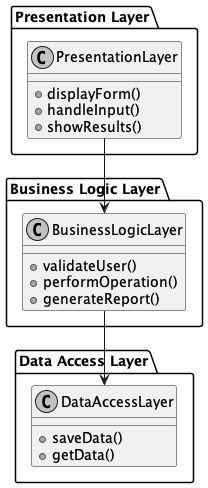
\includegraphics[width=0.25 \textwidth]{fig/uml/simple-layers.png}
  \caption{Einfaches Schichtenmodell}
  \label{fig:simple-layer}
\end{figure}

In dem Beispiel \ref{fig:simple-layer} sind drei Schichten beschrieben, die jeweils eine Schicht darstellen:
\begin{itemize}
\item Das \enquote{Presentation Layer} enthält die Klasse "PresentationLayer", die für die Benutzeroberfläche und die Interaktion mit dem Benutzer zuständig ist.

\item Das \enquote{Business Logic Layer} enthält die Klasse "BusinessLogicLayer", die die Geschäftslogik und die Regeln enthält, die die Anwendung ausführen.

\item Das \enquote{Data Access Layer} enthält die Klasse \enquote{DataAccessLayer}, die für den Zugriff auf Datenbanken oder andere Datenquellen zuständig ist.
\end{itemize}
Die Pfeile zwischen den Komponenten zeigen die Abhängigkeiten zwischen den Schichten an. Die Presentation Layer ist von der Business Logic Layer abhängig und die Business Logic Layer ist von der Data Access Layer.
\\\\
Ein \enquote{Tier} hingegen beschreibt die physische oder logische Aufteilung von Anwendungen oder Systemen auf verschiedene Server oder Endgeräte. Jedes Tier hat normalerweise eine spezifische Funktion, wie z.B. Datenbank-Tier, Anwendungs-Tier oder Präsentations-Tier. Die Tiers sind normalerweise durch eine Netzwerkverbindung miteinander verbunden, und jede Schicht kommuniziert direkt mit der Schicht darüber oder darunter.
\begin{figure}[!h]
  \centering
  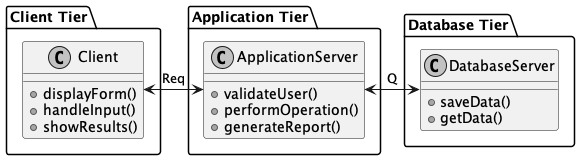
\includegraphics[width=0.80\textwidth]{fig/uml/simple-tiers.png}
  \caption{Einfaches Tier Modell}
  \label{fig:simple-tier}
\end{figure}
In diesem Beispiel haben wir drei Komponenten, die jeweils ein Tier darstellen:
\begin{itemize}
\item Das \enquote{Client Tier} enthält die Klasse \enquote{Client}, die für die Benutzeroberfläche und die Interaktion mit dem Benutzer auf dem Client-Gerät zuständig ist.

\item Das \enquote{Application Tier} enthält die Klasse \enquote{ApplicationServer}, die die Geschäftslogik und die Regeln enthält, die die Anwendung auf dem Application Server ausführen.

\item Das \enquote{Database Tier} enthält die Klasse \enquote{DatabaseServer}, die für den Zugriff auf Datenbanken oder andere Datenquellen auf dem Database Server zuständig ist.
\end{itemize}
Die Pfeile zwischen den Komponenten zeigen die Kommunikation zwischen den Tiers an. Der Client sendet eine Anfrage an den Application Server und der Application Server leitet die Anfrage an den Database Server weiter. Der Database Server gibt dann eine Antwort zurück, die über den Application Server an den Client zurückgesendet wird.
\\\\

Im Zweifel können Tiers und Layers die gleichen Namen besitzen, obwohl sich Ihre Motivation im Design unterschiedet. Vielleicht hilft auch nochmal die Sicht auf die Ziele der unterschiedlichen Zuschnitte. Im Layer-Modell sind folgende Ziele eher mit dem gewünschten Zuschnitt verbunden:
\begin{itemize}
\item Bestimmung der Funktionen und die Zuordnung zu logischen Komponenten mit fester Verantwortung und festen Schnittstellen. 
\item Bessere Wartbarkeit und die Flexibilität bei der Ausgestaltung. Komponenten können ausgetauscht und ersetzt werden, da sie festen Schnittstellendefinitonen genügen.  
\end{itemize}
Der Fokus auf die Tiers adressiert mehr die physischen Anforderung an die Architektur des verteilten Systems. Vielleicht sind daher folgende Ziele eher mit dem Tier-Model verbunden:
\begin{itemize}
\item Bestimmung der möglichen Skalierung auf (logische/virtuelle) Hardware und die generelle Zusweisung der logischen Komponenten.
\item Bestimmung der (Netzwerk-)Charakteristiken für die Kommunkation zwischen den Komponenten.
\end{itemize}
Ein besonderer Architekturtyp ist ein \enquote{Single-Node-Application}, welcher in einem Verteilten System als 1-Tier-Architektur verstanden werden kann.

\subsubsection{Single Node}

Eine Single-Node-Application ist ein Architekturtyp der das Ziel hat, das Anwendung auf einem einzelnen Knoten in einem verteilten System ausgeführt werden. Im Gegensatz zu einer Anwendung, die auf mehreren Knoten ausgeführt wird braucht es hier keine Verteilung der Funktionen oder Daten über den logischen/physikalischen Knoten hinaus. Der Knoten kann ein physischer Server oder eine virtuelle Maschine sein.

Ein Beispiel für eine Single-Node-Application in einem verteilten System könnte eine Anwendung sein, die Daten von verschiedenen Systemen sammelt und verarbeitet. Obwohl die Anwendung nur auf einem Knoten ausgeführt wird, muss sie möglicherweise mit verschiedenen Systemen und Datenquellen kommunizieren, dies ist in der Architektur nicht nur nicht ausgeschlossen, sondern eine erwünschte Eigenschaft.

Obwohl Single-Node-Applications nicht auf mehreren Knoten verteilt sind, können sie daher immer noch von den Vorteilen von verteilten Systemen profitieren, wie z.B. Skalierbarkeit, Zuverlässigkeit und Flexibilität. 
Single-Node-Applications können auch von der Verwendung von Middleware-Technologien wie Message Queues und RPC profitieren, die die Interoperabilität zwischen verschiedenen Anwendungen und Systemen erleichtern, die Middleware wird aber nicht primär für die kooperative Arbeit genutzt, sonder für das Sammeln und Aufbereiten der Daten. Diese Überlegungen münden in die Bestrebung der Formulierung eines Best Practice Entwurfmusters (Pattern): Single-Node-Pattern.
Das Single-Node-Pattern kann in verschiedenen Szenarien nützlich sein, wie zum Beispiel:
\begin{itemize}
\item Entwicklung und Testen: Das Single-Node-Pattern kann verwendet werden, um Anwendungen auf einem einzigen Knoten während der Entwicklung und Tests auszuführen, um Zeit und Ressourcen zu sparen, die für die Bereitstellung und Verwaltung von verteilten Systemen erforderlich sind.
\item Kleine Anwendungen: Das Single-Node-Pattern kann nützlich sein, wenn die Anwendung klein ist und nicht viele Ressourcen benötigt. In diesem Fall kann eine Single-Node-Implementierung ausreichend sein, um die Anforderungen der Anwendung zu erfüllen.
\item Datenintensive Anwendungen: Das Single-Node-Pattern kann auch für datenintensive Anwendungen nützlich sein, bei denen die Daten auf einem einzigen Knoten gespeichert und verarbeitet werden können.
\end{itemize}
Das Single-Node-Pattern kann mit verschiedenen Technologien implementiert werden, wie z.B. Container-Technologien (Docker), virtuelle Maschinen (VMs) oder Serverless-Computing (AWS Lambda). Die Wahl der Technologie hängt von den Anforderungen der Anwendung und den verfügbaren Ressourcen ab.

Das Single-Node-Pattern bezieht sich auf die Verwendung eines einzigen Serverknotens oder einer einzelnen Instanz eines Dienstes, anstatt mehrere Knoten zu verwenden, um denselben Dienst bereitzustellen. Hier sind einige Beispiele von Unternehmen, die dieses Muster einsetzen:
\begin{itemize}
\item Netflix: Netflix verwendet das Single-Node-Pattern, um die Datenverarbeitung in ihren AWS-Cloud-Instanzen zu optimieren. Sie haben sich dafür entschieden, ihre Anwendungen in kleinere, spezialisierte Dienste aufzuteilen, die auf einzelnen Knoten ausgeführt werden. Dies ermöglicht es ihnen, schnell auf Anforderungen zu reagieren, ohne Ressourcen für überflüssige Knoten zu verschwenden.
\item Airbnb: Airbnb verwendet das Single-Node-Pattern, um ihre Webanwendung (Nicht die Daten) in einem einzigen Knoten zu hosten, anstatt sie auf mehrere Knoten aufzuteilen. Durch die Verwendung eines einzigen Knotens ist die Anwendung einfacher zu verwalten und zu skalieren. Airbnb kann schnell auf Veränderungen in der Nachfrage reagieren und ihre Anwendung schnell anpassen.
\end{itemize}

Für die weitere Diskussion müssen die physikalischen oder auch logischen Verbindung zwischen Nodes diskutiert werden. Die logische Verbindung muss keiner physikalischen Verbindung entsprechen. Diese \enquote{virtuelle} Netzwerkstruktur besteht häufig auf der obersten Schicht einer physikalischen Netzwerkstruktur und wird als Overlay-Netzwerk bezeichnet. Es ermöglicht den Aufbau von Netzwerkdiensten und Anwendungen, die auf verteilten Systemen basieren, indem es zusätzliche Abstraktion und Organisation bietet. Das Ziel eines Overlay-Netzwerks ist es, die Kommunikation und Zusammenarbeit zwischen den Knoten zu verbessern, die Skalierbarkeit zu erhöhen und die Netzwerkverwaltung zu vereinfachen. Sie ermöglichen es, verteilte Anwendungen und Dienste unabhängig von der zugrunde liegenden Netzwerkinfrastruktur zu entwickeln und bereitzustellen. Allerdings können Overlay-Netzwerke auch zusätzliche Komplexität und Overhead verursachen, da sie auf bestehenden Netzwerkstrukturen aufbauen und von diesen abstrahiert sind, daher neigen Entwickler gerne dazu die bereits beschriebenen Fettnäpfchen zu suchen.

Ein Beispiel für ein Overlay-Netzwerk ist das Peer-to-Peer (P2P)-Overlay-Netzwerk~\cite{tanenbaum2017distributed}. In einem P2P-Netzwerk sind die Knoten gleichberechtigte Teilnehmer, die direkt miteinander kommunizieren und Ressourcen wie Rechenleistung, Speicherplatz und Bandbreite teilen. P2P-Netzwerke werden häufig für den Austausch von Dateien, die Verteilung von Inhalten oder die Bereitstellung von Streaming-Diensten verwendet.
Ein bekanntes Beispiel für ein P2P-Overlay-Netzwerk ist das BitTorrent-Protokoll. BitTorrent ermöglicht den verteilten Austausch von Dateien über das Internet, indem es die Dateien in kleinere Teile (sogenannte Chunks) aufteilt und diese über mehrere Peers verteilt. Jeder Peer, der an einem Dateiaustausch teilnimmt, lädt Teile der Datei von anderen Peers herunter und stellt gleichzeitig bereits heruntergeladene Teile für andere Peers zur Verfügung. Auf diese Weise wird die Last auf die einzelnen Knoten im Netzwerk verteilt, und die Geschwindigkeit und Zuverlässigkeit des Dateiaustauschs verbessert.

Strukturierte und unstrukturierte Netzwerke sind zwei verschiedene Ansätze für die Organisation und den Aufbau von verteilten Systemen oder Overlay-Netzwerken. Beide haben ihre eigenen Vor- und Nachteile, abhängig von den Anforderungen und dem Nutzungszweck des Netzwerks.
\begin{itemize} 
\item Organisation: Strukturierte Netzwerke sind durch eine gut definierte und geordnete Struktur gekennzeichnet. Sie verwenden meist deterministische Verfahren oder Algorithmen, um die Verbindungen zwischen den Knoten im Netzwerk herzustellen und aufrechtzuerhalten. Unstrukturierte Netzwerke haben keine festgelegte oder geordnete Struktur. Die Verbindungen zwischen den Knoten im Netzwerk werden zufällig oder auf der Grundlage von Heuristiken hergestellt.
\item Routing: Das Routing in strukturierten Netzwerken ist effizienter und vorhersagbarer, da es auf der Grundlage der Netzwerkstruktur erfolgt. Ein Beispiel für ein strukturiertes Routing-Verfahren ist das Distributed Hash Table (DHT), bei dem die Knoten und Ressourcen auf der Grundlage von Hash-Werten organisiert sind. Im Gegensatz zu strukturierten Netzwerken ist das Routing in unstrukturierten Netzwerken weniger effizient und vorhersagbar. Die Nachrichten können mehrere Hops zwischen Knoten benötigen, um ihr Ziel zu erreichen, und es kann zu einer höheren Netzwerkbelastung führen.
\item Suche: In strukturierten Netzwerken ist die Suche nach Ressourcen oder Knoten meist schneller, da sie auf vordefinierten Pfaden und Algorithmen basiert. Die Suche kann in logarithmischer Zeit (O(log N)) durchgeführt werden, wobei N die Anzahl der Knoten im Netzwerk ist. Die Suche in unstrukturierten Netzwerken erfolgt meist über Flooding- oder Random-Walk-Verfahren, bei denen eine Anfrage an mehrere Knoten gleichzeitig gesendet wird. Dies kann zu längeren Suchzeiten und höherer Netzwerkbelastung führen, insbesondere in großen Netzwerken.
\item Skalierbarkeit: Strukturierte Netzwerke sind im Allgemeinen besser skalierbar und eignen sich für große, verteilte Systeme, da die Organisation und das Routing effizienter gestaltet sind.
Unstrukturierte Netzwerke sind in der Regel weniger skalierbar als strukturierte Netzwerke, da sie anfälliger für Netzwerkengpässe und ineffizientes Routing sind. Sie eignen sich jedoch für kleinere Netzwerke oder Anwendungen, bei denen eine flexible und dynamische Organisation wichtiger ist als Effizienz.
\end{itemize} 
Aber nicht nur die Struktur stellt das Design vor unterschiedliche Herausforderungen, auch die Einordnung in bekannte und unbekannte Kommunikationspartner und wie man diese in Gruppen organisiert oder Resourcen auch vor schädlichen Teilnehmern schützt.

\subsubsection{Middleware Architektur}
Neben dem Bedürfnis der Verteilung steht auch die Kapslung der Aufgabe im Fokus. So wäre es zielgerichtet, nach den bisherigen Diskussionen, eine Schicht zu kreieren, welche die Aufgaben der Verteilung in sich vereint.
\cite{tanenbaum2017distributed} beschreibt die Aufgaben der Schicht mit:
\begin{itemize}
\item Bereitstellung eines breiten Angebotes für die Kommunikation: 
Eine wichtige Funktion der Middleware ist die Bereitstellung eines umfangreichen Satzes von Kommunikationsprotokollen, die die Interaktion zwischen verschiedenen Anwendungen und Systemen ermöglichen. Diese Protokolle stellen sicher, dass Daten zwischen verschiedenen Anwendungen und Systemen effizient und sicher ausgetauscht werden können.
\item Dem (Un)Marshaling Prozess: Ein weiterer wichtiger Aspekt von Middleware ist das (Un)Marshaling von Daten, das für integrierte Systeme notwendig ist. (Un)Marshaling bezieht sich auf den Prozess des Konvertierens von Daten in ein Format, das von einer anderen Anwendung oder einem anderen System verwendet werden kann. Die Middleware bietet die notwendigen Mechanismen, um Daten zwischen verschiedenen Systemen in einem Format zu konvertieren, das von allen beteiligten Anwendungen und Systemen verstanden werden kann.
\item Protokolle zur Namensauflösung: Darüber hinaus bieten Middleware-Dienste auch Namensprotokolle, die es ermöglichen, Ressourcen einfach zu teilen. Mit Namensprotokollen können Ressourcen in einem verteilten System mit einem eindeutigen Namen identifiziert und von verschiedenen Anwendungen und Systemen einfach referenziert werden.
\item Sicherheitsprotokolle: Auch ist die Bereitstellung von Sicherheitsprotokollen ein wichtiges Merkmal. Diese Protokolle bieten Mechanismen zur Verschlüsselung von Daten und zur Authentifizierung von Benutzern und Systemen, um sicherzustellen, dass nur autorisierte Benutzer auf das System zugreifen können und dass Daten während der Übertragung verschlüsselt und gesichert sind.
\item Mechanismen zur Steigerung der Skalierung: Schließlich bietet Middleware auch Skalierungsmechanismen wie Replikation und Caching, um die Leistung von Anwendungen in einem verteilten System zu verbessern. Diese Mechanismen ermöglichen die Duplizierung von Daten und Ressourcen auf verschiedenen Systemen, um die Verfügbarkeit und Zuverlässigkeit von Anwendungen zu erhöhen. Diese Punkte werden nochmals genauer in späteren Kapiteln diskutiert.
\end{itemize}
Eine solche Schicht wird als \enquote{Middleware}-Schicht bezeichnet, für den Applikationsentwickler bleibt nur die Entwicklung des Anwendungsprotokolls. Im besten Fall bietet die Schnittstelle der Middlewareschicht ein abstrahiertes \enquote{Interface}, welches sich im besten Fall nicht von einem Standalone System abgrenzen lässt, sich somit verhält wie ein kohärentes System. Das Interface, mit der verbundenen Realisierung hat das primäre Ziel Interoperabilität über verschiedene Systeme herzustellen. Diese Aufgabe kann auch in einzelne Aufgaben geteilt werden: 
\begin{itemize}
\item Mehrere Sprachen unterstützt: Middleware kann verwendet werden, um die Interoperabilität zwischen verschiedenen Anwendungen zu verbessern, die in verschiedenen Programmiersprachen geschrieben sind. Die Middleware kann als Übersetzungsschicht dienen, um Nachrichten zwischen den Anwendungen zu übersetzen und sicherzustellen, dass sie in der korrekten Syntax und Semantik gesendet und empfangen werden.
\item Mit mehreren Betriebssystemen und Hardwaretypen arbeitet: Eine Middleware kann dazu beitragen, die Interoperabilität zwischen Anwendungen zu verbessern, die auf verschiedenen Betriebssystemen und Hardwaretypen ausgeführt werden. Die Middleware kann als eine Abstraktionsschicht dienen, die es den Anwendungen ermöglicht, unabhängig von der zugrunde liegenden Hardware und dem Betriebssystem zu arbeiten.
\item Mehrere Netzwerkprotokolle unterstützt: Middleware kann verwendet werden, um die Interoperabilität zwischen Anwendungen zu verbessern, die verschiedene Netzwerkprotokolle verwenden. Die Middleware kann als eine Schicht dienen, die es den Anwendungen ermöglicht, Nachrichten in einem bestimmten Protokoll zu senden und zu empfangen, unabhängig davon, welches Protokoll von der anderen Anwendung verwendet wird.
\end{itemize}
Um die Kommunikation innerhalb eine Middleware-Schicht zu realisieren ergeben sich unterschiedliche Ansätze für die Kommunikation, die zuächst kurz eingeführt werden sollen. Diese Alternativen haben auch über die Middleware hinaus Gültigkeit.  
\begin{itemize}
\item Point to point\\
Die Point-to-Point-Kommunikation kann in einem verteilten System auf verschiedene Arten implementiert werden, wie zum Beispiel durch die Verwendung von Messaging-Systemen oder direkter Socket-Kommunikation. In beiden Fällen muss der Absender die Adresse des Empfängers kennen, um die Nachricht zu senden.

Point-to-Point-Nachrichten werden häufig verwendet, um bestimmte Aufgaben oder Transaktionen zwischen verschiedenen Komponenten oder Diensten in einem verteilten System auszuführen. Zum Beispiel kann eine Anwendung eine Point-to-Point-Nachricht senden, um eine Anforderung an einen anderen Dienst im System zu stellen, um eine bestimmte Aktion auszuführen oder eine Antwort auf eine Anfrage zu erhalten.Vorteile von Point-to-Point-Nachrichten sind unter anderem:
\begin{itemize}
\item Effizienz: Point-to-Point-Nachrichten sind effizienter als Multicast/ Broadcast-Nachrichten auf einem Medium das primär dezidierte Kommunikation zwischen zwei Kommunikationspartner ermöglicht. Der Aufwand ist dann gering, da sie nur an einen spezifischen Empfänger gesendet werden, der die Nachricht empfangen soll. Im besten Fall ist nichtmal eine Addressierung notwendig.
\item Präzision: Point-to-Point-Nachrichten sind präziser als Broadcast-Nachrichten, da sie nur an den Empfänger gesendet werden, der die Nachricht empfangen soll, was das Risiko von Konflikten oder Fehlern verringert. Sie können auch für einen bestimmten Empfänger oder Sender optimiert werden.
\end{itemize} 
Wichtig an dem Beispiel in \ref{lst:p2p-message} ist, dass in diesem Fall die Middleware sich über die Nachricht bewusst sein muss. Es werden noch generischere Ansätze diskutiert werden, wo die Middleware keine Annahmen über die Nachricht selbst formuliert. 

Bei der Kodierung von Nachrichten können verschiedene Freiheitsgrade genutzt werden. Eine Auswahl von Beispielen sollen an dem Fallbeispiel der Lampe besprochen werden. Zur Steuerung einer Lampenschaltung gibt es verschiedene Möglichkeiten, je nach Komplexität der Anforderungen und der verwendeten Kommunikationstechnologie. Hier sind einige Beispiele für verschiedene Codierungsansätze:
\newpage
\begin{lstlisting}[caption={Message für Point to Point Kommunikation},captionpos=b,label={lst:p2p-message}]
{
   "message_id": "12345",
   "sender": "applicationA",
   "receiver": "applicationB",
   "payload": {
      "command": "update_customer",
      "customer_id": "67890",
      "data": {
         "first_name": "John",
         "last_name": "Doe",
         "email": "johndoe@example.com"
      }
   }
}
\end{lstlisting}

\begin{itemize}
\item Binäre Codierung (0 und 1): Die einfachste Form der Codierung besteht darin, die Lampe mit einem einzigen Binärwert zu steuern. Eine "0" könnte "Lampe aus" bedeuten, während eine "1" "Lampe an" bedeutet. Dieser Ansatz ist sehr einfach und eignet sich für grundlegende Anwendungen, bei denen nur ein- oder ausgeschaltet werden muss.
\item Zeichenketten (Text): Eine andere Möglichkeit ist die Verwendung von Zeichenketten zur Codierung von Nachrichten. Zum Beispiel könnte die Nachricht \enquote{ON} verwendet werden, um die Lampe einzuschalten, und \enquote{OFF}, um sie auszuschalten. Dieser Ansatz ist etwas ausführlicher als die Binärcodierung, ermöglicht aber auch eine einfachere Interpretation und Erweiterbarkeit, wenn zusätzliche Funktionen hinzugefügt werden müssen.
\item Enumerations: Für eine klarere Struktur und Typsicherheit können Enumerations verwendet werden. Enums definieren einen Satz von benannten Werten, die die möglichen Zustände der Lampe darstellen. Zum Beispiel: \enquote{LAMPE\_AN} und \enquote{LAMPE\_AUS}. Dieser Ansatz ist gut lesbar und ermöglicht eine leichtere Erweiterung bei der Hinzufügung neuer Funktionen.
\item TLV\footnote{Typ Length Value} Strukturen: Für komplexere Anwendungen, in denen mehrere Attribute oder Parameter beteiligt sein können, können TLV-Strukturen verwendet werden. In einer TLV-Struktur wird jeder Parameter durch einen Typ, eine Länge und einen Wert dargestellt. Zum Beispiel könnte der Typ \enquote{1} für die Lampensteuerung verwendet werden, die Länge gibt die Anzahl der Bytes für den Wert an und der Wert selbst repräsentiert den gewünschten Zustand der Lampe (z. B. \enquote{0} für aus, \enquote{1} für an). TLV-Strukturen sind flexibel, erweiterbar und eignen sich gut für verteilte Systeme und komplexe Anwendungen.
\end{itemize}

\item Point to multipoint: Eine Point-to-Multipoint Koomunikation zeichnet sich dadurch aus, das eine Nachricht von einem Absender an mehrere Empfänger in einem verteilten System gesendet wird. 

Ein Beispiel für eine Point-to-Multipoint-Nachricht wäre eine Nachricht, die an eine Gruppe von Abonnenten in einem Nachrichtenbroker-System gesendet wird. Der Absender sendet die Nachricht an den Broker, der die Nachricht dann an alle Abonnenten weiterleitet, die diese spezifische Nachricht abonniert haben.

Ein anderes Beispiel wäre ein System zur Überwachung von Sensoren in einer Fabrik. Der Absender kann eine Point-to-Multipoint-Nachricht an alle Sensoren senden, um ein Update der Einstellungen oder einen Alarm zu senden, anstatt eine Point-to-Point-Nachricht an jeden Sensor einzeln zu senden. Vorteile von Point-to-Multipoint-Nachrichten sind unter anderem:
\begin{itemize}
\item Effizienz: Point-to-Multipoint-Nachrichten sind effizienter als Point-to-Point-Nachrichten auf Übertragungsmedien die inhärent Boradcast sind bzw. Strukturen und Komponenten für diese Kommunikation vorsehen, da sie an mehrere Empfänger gleichzeitig gesendet werden können und somit die Netwerklast reduzieren können.
\item Skalierbarkeit: Point-to-Multipoint-Nachrichten sind skalierbar und können in verteilten Systemen mit vielen Empfängern verwendet werden.
\item Einfache Implementierung: Point-to-Multipoint-Nachrichten können einfach implementiert werden, da sie in vielen Messaging-Systemen und Protokollen unterstützt werden.
\item Schnellere Verarbeitung: Point-to-Multipoint-Nachrichten können schneller verarbeitet werden als Point-to-Point-Nachrichten, da sie nur einmal gesendet werden müssen, anstatt an jeden Empfänger einzeln.
\end{itemize}
Point-to-Multipoint-Nachrichten sind ein wichtiger Bestandteil von verteilten Systemen und bieten insbesondere im Kontext der Replikation große Vorteile.
\item Event/action: Diese Art der Kommunikation beschreibt mehr den Mechanismus bei der Kommunikation. So kann man die notwendigen Elemente in 5 Punkte beschreiben:
\begin{itemize}
\item Ereignisquellen: Ereignisquellen sind Dienste oder Komponenten in einem verteilten System, die Ereignisse, den Event, erzeugen und an das System senden können. Diese Ereignisse können von verschiedenen Arten sein, z.B. Benutzeraktionen, Systemmeldungen oder Datenaktualisierungen.
\item Ereignisverarbeitung: Ereignisverarbeitung ist der Mechanismus, mit dem Ereignisse im verteilten System erfasst, verarbeitet und in einen Zustand umgewandelt werden, der für die weiteren Aktionen verwendet werden kann. Dies kann beinhalten, die Ereignisse zu filtern, zu transformieren oder zu aggregieren.
\item Ereignisrouting: Ereignisrouting ist der Mechanismus, mit dem Ereignisse an die richtigen Dienste oder Komponenten im verteilten System weitergeleitet werden. Dies kann durch die Verwendung von Routing-Regeln, Ereignisfiltern oder anderen Methoden erfolgen.
\item Ereignisempfang: Ereignisempfang ist der Mechanismus, mit dem Ereignisse von verschiedenen Quellen im verteilten System empfangen werden können. Dies kann durch die Verwendung von APIs, Messaging-Systemen oder anderen Methoden erfolgen.
\item Ereignisreaktion: Ereignisreaktion ist der Mechanismus, mit dem das System auf Ereignisse reagiert, die empfangen wurden. Dies kann die Ausführung von Aktionen, die Aktualisierung von Daten oder die Weiterleitung von Ereignissen an andere Komponenten oder Dienste beinhalten.
\end{itemize}
Wichtig ist in diesem Kontext zu verstehen, das, obwohl die Kombination Event/Aktion sehr intuitiv erscheint, die dafür notwendigen Konstruktionen sehr aufwendig sein können. Insbesondere das Ereignisrouting kann eine hohe Komplexität einnehmen. 

\item Publish/subscribe: Publish/Subscribe ist ein Kommunikationsform, bei dem Komponenten oder Dienste sich für bestimmte Ereignisse oder Nachrichten anmelden und dann automatisch benachrichtigt werden, wenn diese Ereignisse oder Nachrichten auftreten.

Das Muster besteht aus zwei Hauptkomponenten: dem Publisher und dem Subscriber. Der Publisher ist für das Erzeugen und Senden von Ereignissen oder Nachrichten an das System verantwortlich. Der Subscriber ist für das Abonnieren von Ereignissen oder Nachrichten und für das Empfangen von Benachrichtigungen über diese Ereignisse oder Nachrichten verantwortlich. Das genutzte Publish/Subscribe-Pattern ermöglicht eine lose Kopplung zwischen dem Publisher und dem Subscriber. 

Der Publisher muss nicht wissen, wer die Ereignisse oder Nachrichten empfängt, und der Subscriber muss nicht wissen, woher die Ereignisse oder Nachrichten kommen. Dies ermöglicht eine höhere Flexibilität und Skalierbarkeit des Systems, da neue Komponenten oder Dienste einfach hinzugefügt oder entfernt werden können, ohne dass dies Auswirkungen auf andere Komponenten oder Dienste hat.

Das Muster kann auf verschiedene Arten implementiert werden, z.B. durch die Verwendung von Messaging-Systemen, die die Kommunikation zwischen dem Publisher und dem Subscriber verwalten, oder durch die Verwendung von APIs, die es dem Subscriber ermöglichen, Ereignisse oder Nachrichten direkt vom Publisher zu empfangen.

Ein Beispiel für die Verwendung von Publish/Subscribe ist ein System zur Überwachung von Sensoren in einer Fabrik. Die Sensoren senden Ereignisse an das System, wenn sie ein Problem erkennen. Die verschiedenen Komponenten des Systems, wie z.B. das Alarmierungssystem oder das Wartungssystem, abonnieren diese Ereignisse und werden automatisch benachrichtigt, wenn ein Problem auftritt. Dadurch kann das System schnell auf Probleme reagieren und effizienter arbeiten.

Wichitg wahrzunehmen ist, dass die Realisierung eines Publish/Subscribe meist selbst ein verteiltes System darstellt und meist über Point-to-Point oder Point-to-Multipoint kommuniziert.
\item Client/Server, Request/Reply\\
Neben dem später diskutierten Client/Server-Archtekturmuster, existiert auch das Client/Server Kommunikationsmuster. Das Client/Server-Kommunikations-muster ist ein grundlegendes Pattern in der Entwicklung von Netzwerkanwendungen, bei dem eine Anwendung (der Client) eine Verbindung zu einer anderen Anwendung (dem Server) herstellt, um eine bestimmte Aktion oder Dienstleistung anzufordern.

In diesem Muster sendet der Client eine Anfrage an den Server, die eine bestimmte Aktion oder ein bestimmtes Ergebnis erfordert. Der Server verarbeitet die Anfrage und sendet eine Antwort zurück an den Client, die das Ergebnis der Anfrage enthält.

Das Client/Server-Kommunikationsmuster ermöglicht es, komplexe Anwendungen aufzubauen, indem verschiedene Komponenten oder Dienste in einem verteilten System miteinander kommunizieren. Der Client kann verschiedene Anfragen an den Server senden, z.B. die Abfrage von Daten oder die Ausführung von Operationen, und der Server kann entsprechend antworten und die angeforderten Dienste bereitstellen.

Das Muster kann auf verschiedene Arten implementiert werden, z.B. durch die Verwendung von APIs, die es dem Client ermöglichen, Anfragen direkt an den Server zu senden, oder durch die Verwendung von Messaging-Systemen, die die Kommunikation zwischen dem Client und dem Server verwalten.

Ein Beispiel für die Verwendung des Client/Server-Kommunikationsmusters ist eine Webanwendung, bei der ein Benutzer eine Anfrage an einen Webserver sendet, um eine bestimmte Webseite anzuzeigen. Der Webserver verarbeitet die Anfrage und sendet die entsprechende Webseite an den Browser des Benutzers zurück.

In diesem Fall wird sogar duch die Nutzung des HTTP Protokolls, das Request/Reply-Muster angewendet, welches eine spezielle Form der Client/Server-Kommunikation beschreibt. In diesem Fall wird immer in einer synchronen Kommunikation eine Anfrage (Request) gestellt und auf die Antwort (Reply/Response) gewartet. Andere Client/Server-Kommunikationsmuster können auch asynchron sein.

Das Client/Server-Kommunikationsmuster ist eine effektive Möglichkeit, verteilte Anwendungen zu entwickeln, indem es eine einfache Methode zur Kommunikation zwischen verschiedenen Komponenten und Diensten bietet. Basis der Kommunikation kann eine Point-to-Point, Point-to-Multipoint aber auch Publish/Subscribe Kommunikations sein. 

\item Mobile code\\
Mobile Code ist ein Konzept in verteilten Systemen, bei dem ein Stück Code von einem Computer zu einem anderen Computer transportiert und auf diesem ausgeführt wird. Der Code wird dabei in der Regel als ausführbare Datei oder Skript über das Netzwerk übertragen.

Mobile Code ermöglicht es, Anwendungen und Dienste zu entwickeln, die auf verteilten Systemen ausgeführt werden können. Ein Beispiel für die Verwendung von Mobile Code ist die Remote-Ausführung von Skripten oder Programmen auf einem Server, der von einem Client-Computer aus gesteuert wird. Ein weiteres Beispiel ist die Verwendung von JavaScript in Webbrowsern, bei denen der Code von einer Website heruntergeladen und auf dem Client-Computer ausgeführt wird.

Ein aktuelles Beispiel für die Verwendung von Mobile Code ist die Verwendung von Container-Technologien wie Docker oder Kubernetes. Container können als mobile Code betrachtet werden, da sie Anwendungen und deren Abhängigkeiten in einem einzigen Paket bündeln und es ermöglichen, diese auf verschiedenen Computern und Betriebssystemen auszuführen. Container-Images können auf einem Server erstellt und dann auf andere Server oder Cloud-Plattformen verteilt werden, wo sie ausgeführt werden können.

Mobile Code birgt jedoch auch Risiken, da er Sicherheitsprobleme wie die Möglichkeit der Einschleusung von Malware oder Viren auf dem Zielcomputer aufgrund fehlender Kontrolle über den ausgeführten Code verursachen kann. Es ist wichtig, geeignete Sicherheitsmechanismen und Überprüfungsverfahren zu implementieren, um diese Risiken zu minimieren.

Für die Übertragung von Mobile Code braucht es wieder rudimentärere Kommunikationsmuster. 
\item Virtual shared \\
Virtual Shared Memory (VSM) ist ein Konzept in verteilten Systemen, das es mehreren Prozessen ermöglicht, auf gemeinsamen Speicher zuzugreifen, als ob sie physisch auf demselben Computer ausgeführt würden. Dabei wird ein virtueller Adressraum bereitgestellt, der auf mehreren Computern verteilt ist, aber für die Prozesse so aussieht, als ob er auf einem einzigen Computer lokalisiert wäre.

Das VSM-Konzept ermöglicht es, die Kommunikation und den Datenaustausch zwischen verschiedenen Prozessen in einem verteilten System zu optimieren, indem der gemeinsame Speicher für alle Prozesse zugänglich gemacht wird. Dadurch können die Prozesse auf Daten zugreifen und sie teilen, ohne dass explizite Nachrichtenübertragungsprotokolle erforderlich sind.

Ein Beispiel für die Verwendung von VSM könnte ein verteiltes Datenverarbeitungssystem sein, bei dem mehrere Prozesse gleichzeitig auf Daten in einem gemeinsamen Speicher zugreifen und sie verarbeiten. Statt Daten hin- und herzusenden, können die Prozesse auf den gemeinsamen Speicher zugreifen, um auf die benötigten Daten zuzugreifen und sie zu verarbeiten.

Eine weitere Anwendung von VSM könnte in der Cloud-Computing-Umgebung sein, wo virtuelle Maschinen auf verschiedenen physischen Servern ausgeführt werden. Wenn eine virtuelle Maschine den Zugriff auf Speicher benötigt, der auf einem anderen Server lokalisiert ist, kann VSM verwendet werden, um den Zugriff auf den gemeinsamen Speicher zu ermöglichen, als ob er auf der lokalen Maschine vorhanden wäre.

Die darunterliegende Technologie, kann aber auch wieder als verteiltes System verstanden werden.
\end{itemize}
Mit welchen Kommuikationsansatz das verteilte System in der Middleware auch umgesetzt wird, die vielen Vorteile für den Anwendungsentwickler bleiben davon unberührt. Hier sind einige davon:
\begin{itemize}
\item Abstraktion von Komplexität: Die Middleware abstrahiert die Komplexität der unterliegenden Systeme und Technologien und bietet Entwicklern eine einheitliche Schnittstelle zum Entwickeln von Anwendungen. Dadurch müssen Entwickler nicht jedes Mal neu lernen, wie sie mit verschiedenen Technologien und Systemen arbeiten müssen, sondern können sich auf das Entwickeln der eigentlichen Anwendung konzentrieren.

\item Erhöhte Produktivität: Die Middleware bietet viele vorgefertigte Komponenten und Bibliotheken, die Entwickler in ihren Anwendungen verwenden können. Dadurch können sie die Entwicklung beschleunigen und sich auf die Funktionen konzentrieren, die für ihre Anwendung einzigartig sind.

\item Flexibilität: Die Middleware bietet Entwicklern eine flexible und erweiterbare Architektur, die es ihnen ermöglicht, ihre Anwendungen schnell an sich ändernde Anforderungen anzupassen.

\item Interoperabilität: Die Middleware bietet eine Plattform für die Interoperabilität zwischen verschiedenen Systemen und Anwendungen. Dadurch können Entwickler Anwendungen entwickeln, die mit verschiedenen Systemen und Technologien kommunizieren können.

\item Zuverlässigkeit: Die Middleware bietet Funktionen für die Überwachung und Fehlerbehebung, um sicherzustellen, dass Anwendungen zuverlässig und fehlerfrei arbeiten.

\item Skalierbarkeit: Die Middleware bietet Funktionen für die Skalierbarkeit von Anwendungen, um sicherzustellen, dass sie mit zunehmender Benutzerzahl und Datenmenge zurechtkommen.
\end{itemize}


Als besondere Form gilt die \enquote{Nachrichtenorientierte Middleware}, auch bekannt als Message Oriented Middleware (MOM). Sie ist eine Form von Middleware, die auf asynchroner oder synchroner Kommunikation basiert und dabei auf Nachrichtenübertragung setzt. Das Format der übertragenen Nachrichten ist nicht festgelegt, aber in der Praxis hat sich XML oder JSON als besonders beliebt erwiesen. MOM unterstützt drei verschiedene Kommunikationsprotokolle:
\begin{itemize}
\item Direkte Kommunikation zwischen Anwendungen (Message Passing)
\item Indirekte Kommunikation über eine Warteschlange (Message Queueing)
\item Herausgeber stellt dem Abonnenten Nachrichten zur Verfügung (Publish \& Subscribe)
\end{itemize}
\subsubsection{Client-Server-Architektur}

Die Client-Server-Architektur ist ein fundamentales Modell für verteilte Systeme und bildet die Basis für viele Anwendungen und Dienste nicht nur im Internet. In dieser Architektur gibt es zwei Hauptkomponenten:

\begin{itemize}
\item Client: Der Client ist eine Anwendung oder ein System, das Dienste von einem Server anfordert. Clients können auf verschiedenen Geräten wie PCs, Smartphones oder Tablets laufen. Typische Beispiele für Clients sind Webbrowser, E-Mail-Clients und Messaging-Anwendungen.

\item Server: Der Server ist eine Anwendung oder ein System, das Dienste für Clients bereitstellt. Server können auf physischen oder virtuellen Maschinen laufen und sind in der Regel darauf ausgelegt, gleichzeitig mehreren Clients zur Verfügung zu stehen. Beispiele für Server sind Webserver, Datenbankserver und E-Mail-Server.
\end{itemize}

Wichtig ist wahrzunehmen, das nicht jede Verteilung eine Client und Server Architektur ist, sondern dass dies mit der Verteilung der Aufgaben verbunden ist. Auf dem Server sind alle Anbieter (Provider) von Diensten vereint und auf den Clients, die Nutzer (Consumer) der Dienste. 

In der Client-Server-Architektur gibt es eine klare Trennung der Zuständigkeiten:
\begin{itemize}
\item Anfrage und Antwort: Clients stellen Anfragen an Server, die diese verarbeiten und darauf antworten. Die Kommunikation zwischen Client und Server kann über verschiedene Protokolle wie HTTP, FTP oder SMTP erfolgen. Dieses Muster passt auch gut zu einem Request/Reply Pattern. 
\item Ziel der Architektur: Falls möglich Zustandslosigkeit: In vielen Fällen sind Server zustandslos, d.h., sie speichern keine Informationen über den aktuellen Zustand eines Clients zwischen den Anfragen. Dies ermöglicht eine bessere Skalierbarkeit und Wartbarkeit der Server, da sie keine Ressourcen für die Verwaltung von Client-Zuständen aufwenden müssen. Dies macht das Design eines Systems bei weitem einfacher. Zustandsbehaftete Dienste sind schwerer zu beschreiben, zu betreiben und zu warten. 
\item Skalierbarkeit: Die Client-Server-Architektur ermöglicht eine horizontale Skalierung, indem zusätzliche Server hinzugefügt werden, um die Last von einer wachsenden Anzahl von Clients zu bewältigen. Load-Balancer können verwendet werden, um die Last gleichmäßig auf mehrere Server zu verteilen.
\item Zentralisierung: Die zentrale Verwaltung von Ressourcen und Diensten auf dem Server erleichtert die Wartung und Aktualisierung von Anwendungen. Allerdings kann diese Zentralisierung auch zu Engpässen und Single Points of Failure führen, wenn der Server überlastet ist oder ausfällt.
\end{itemize}
Einige Beispiele für Client-Server-Anwendungen:
\begin{itemize}
\item Webanwendungen: Webbrowser (Client) stellen Anfragen an Webserver (Server), die HTML-Dateien, Bilder und andere Ressourcen zurückgeben. Die Kommunikation erfolgt typischerweise über das HTTP- oder HTTPS-Protokoll.
\item E-Mail-Systeme: E-Mail-Clients (z.B., Microsoft Outlook, Apple Mail) stellen Anfragen an E-Mail-Server (z.B., IMAP-, POP3- oder SMTP-Server) zum Senden, Empfangen und Verwalten von E-Mails.
\item Datenbankanwendungen: Anwendungen (Client) stellen Anfragen an Datenbankserver (Server), um Daten zu lesen, schreiben oder aktualisieren. Die Kommunikation erfolgt über Protokolle wie SQL oder NoSQL.
\end{itemize}
Die Client-Server-Architektur und Tiers sind in verteilten Systemen eng miteinander verbunden. Die Client-Server-Architektur bezieht sich auf die Aufteilung der Funktionalität eines Systems zwischen einem Front-End-Client und einem Back-End-Server. In diesem Sinne kann eine Server-Client Architektur auch als Two-Tier-Architektur verstanden werden. Die n-Tier-Architektur erweitert das Konzept, indem sie die Schichten weiter aufteilt und somit noch mehr Flexibilität und Skalierbarkeit ermöglicht. So können in verteilten Systemen unterschiedliche Ausprägungen vorzufinden sein. 
\begin{itemize}

\item Kaskadenartige Kommunikation\\
In einer n-Tier-Architektur können Tiers sowohl Consumer- als auch Provider-Rollen übernehmen, indem sie verschiedene Funktionen und Verantwortlichkeiten innerhalb einer Anwendung repräsentieren und Dienste sowohl anfordern als auch bereitstellen. Die kaskadenartige Kommunikation zwischen den Tiers kann sowohl Vorteile als auch Herausforderungen mit sich bringen.

Wo die Vorteile noch trivial sind, lohnt der genauere Blick auf die Herausforderungen: 
\begin{itemize}
\item Latenz: Die kaskadenartige Kommunikation zwischen Tiers kann zu erhöhter Latenz führen, da jede Schicht auf die Antwort der nächsten Schicht warten muss, bevor sie ihre Arbeit fortsetzen oder abschließen kann.
\item Komplexität: Die Kommunikation zwischen den verschiedenen Tiers kann die Gesamtkomplexität einer Anwendung erhöhen, da zusätzliche Schnittstellen und Protokolle benötigt werden, um die Kommunikation zwischen den Schichten zu ermöglichen.
\item Fehleranfälligkeit: Durch die kaskadenartige Kommunikation kann die Anfälligkeit für Fehler steigen, da ein Problem in einer Schicht sich auf alle anderen Schichten auswirken und die gesamte Anwendung beeinträchtigen kann.
\item Skalierbarkeit: Die kaskadenartige Kommunikation kann die Skalierbarkeit einer Anwendung beeinträchtigen, da die Leistungsfähigkeit einer Schicht von der Leistungsfähigkeit der darunterliegenden Schichten abhängt.
\end{itemize}
Um diesen Herausforderungen zu begegnen, können Entwickler Techniken wie Caching, Lastverteilung, asynchrone Kommunikation und fehlertolerante Mechanismen einsetzen, um die Leistung, Zuverlässigkeit und Skalierbarkeit der Anwendung zu verbessern.

\item SSP - Stub/Skeleton Chains\\
In einer n-tiered Architektur werden oft Stubs und Skeletons eingesetzt, um die Kommunikation zwischen den verschiedenen Schichten oder Tiers zu erleichtern. Stubs und Skeletons sind eine Implementierungsform von Interface-Definitionen, die es ermöglichen, Methodenaufrufe von einer Schicht zur anderen zu senden.

Ein Stub ist ein Platzhalter für eine entfernte Methode. Es stellt eine lokale Implementierung einer Schnittstelle dar, die einen entfernten Server aufruft, um die Funktion auszuführen. Wenn ein Stub aufgerufen wird, wird die Anfrage an den entfernten Server gesendet, und das Ergebnis wird zurück an den Stub gesendet, der dann das Ergebnis an den Aufrufer zurückgibt.

Ein Skeleton ist das Gegenstück zum Stub. Es ist eine Platzhalter-Implemen-tierung für eine lokale Methode, die von einem entfernten Client aufgerufen wird. Ein Skeleton empfängt die Anfrage vom entfernten Client, ruft die entsprechende Methode in der lokalen Implementierung auf und sendet das Ergebnis zurück an den entfernten Client.

In einer n-tiered Architektur werden oft SSP (Service Specific Protocol) Stub/Skeleton Chains verwendet, um die Kommunikation zwischen den verschiedenen Schichten zu erleichtern. SSP Stub/Skeleton Chains sind eine Sequenz von Stubs und Skeletons, die für die Kommunikation zwischen verschiedenen Tiers oder Schichten verwendet werden.

Die SSP Stub/Skeleton Chains helfen dabei, eine gemeinsame Sprache zwischen verschiedenen Schichten oder Tiers zu schaffen. Jeder Stub/Skeleton in der Chain versteht nur das SSP, das von der Schicht darüber und darunter verwendet wird. Auf diese Weise wird sichergestellt, dass die Kommunikation zwischen den Schichten auf eine standardisierte Art und Weise erfolgt, ohne dass jede Schicht die Details der Implementierung der darunterliegenden Schichten kennen muss.
\end{itemize}

\cite{tanenbaum2017distributed} führt als einen wichtigen Aspekt der Client-Server-Architektur die Middleware ein und in die Middleware nimmt er das Konzept der Stub und Skeletons wieder auf. Für \cite{tanenbaum2017distributed} ist eine Middleware insbesondere eine Software, die als Vermittler zwischen Clients und Servern fungiert und hilft, Kommunikation und Interoperabilität in verteilten Systemen zu ermöglichen und Stub und Skeleton sind die Vermittler für die Aufrufe der Funktionen zu diesem Zwecke.
              
\subsubsection{Event-Driven Architektur}

Die Event-Driven Architektur (EDA) ist ein Architekturansatz, bei dem die Kommunikation zwischen den Komponenten eines Systems durch Events oder Nachrichten stattfindet. In einer EDA reagieren die Komponenten auf Ereignisse, die von anderen Komponenten im System generiert werden, anstatt direkt miteinander zu kommunizieren. Dieser Ansatz fördert die Entkopplung und Skalierbarkeit von Anwendungen und ist besonders in Echtzeitsystemen und komplexen, verteilt arbeitenden Umgebungen verbreitet.
\\\\
Beispiel 1: Aktienhandelssystem: Ein Aktienhandelssystem könnte eine EDA verwenden, um auf Ereignisse wie den Kauf oder Verkauf von Aktien zu reagieren. Wenn ein Benutzer eine Aktie kauft, wird ein Kauf-Event generiert und im System verteilt. Andere Komponenten, wie z.B. ein Portfolio-Manager, könnten auf dieses Ereignis reagieren, indem sie das Portfolio des Benutzers aktualisieren. Ebenso könnten weitere Komponenten, wie ein Handelshistorien-Manager, die Handelsaktivitäten aufzeichnen und Analysewerkzeuge die Handelsdaten nutzen, um Handelsempfehlungen zu generieren.
\\\\
Beispiel 2: IoT-Sensornetzwerk: Ein IoT-Sensornetzwerk, das aus vielen Sensoren besteht, die Umgebungsdaten sammeln (z. B. Temperatur, Luftfeuchtigkeit, Luftdruck), könnte eine EDA verwenden, um auf Sensordaten zu reagieren. Wenn ein Sensor neue Daten sammelt, generiert er ein Ereignis, das im System verteilt wird. Andere Komponenten, wie Analysemodule, könnten auf diese Ereignisse reagieren, indem sie die Daten verarbeiten und Entscheidungen treffen, z. B. das Aktivieren von Klimaanlagen bei Überschreiten einer bestimmten Temperatur.
\\\\
Beispiel 3: E-Commerce-Plattform: Eine E-Commerce-Plattform könnte eine EDA verwenden, um auf Ereignisse wie Bestellungen, Warenkorbänderungen und Zahlungen zu reagieren. Wenn ein Kunde eine Bestellung aufgibt, wird ein Bestellungs-Event generiert. Andere Komponenten, wie Lagerverwaltung, Versandabwicklung und Rechnungserstellung, können auf dieses Ereignis reagieren, um den Bestellvorgang abzuschließen. Dies ermöglicht eine asynchrone und flexible Handhabung der Geschäftsprozesse.
\\\\
In einer Event-Driven Architektur sind folgende Komponenten von zentraler Bedeutung:
\begin{itemize}
\item Event-Producer: Komponenten, die Ereignisse generieren und in das System einspeisen.
\item Event-Channel: Eine Kommunikationsinfrastruktur, die Events von Producern zu Consumern transportiert, z. B. Message Broker oder Event Bus.
\item Event-Consumer: Komponenten, die auf bestimmte Ereignisse reagieren und entsprechende Aktionen ausführen.
\end{itemize}
EDA bietet verschiedene Vorteile, wie z. B. lose Kopplung, Skalierbarkeit und Fehlertoleranz. Allerdings gibt es auch Herausforderungen, wie die Komplexität des Event-Handlings, die Nachverfolgbarkeit von Events und die eventuelle Konsistenz in verteilten Systemen.

In einer Even-Driven-Architektur findet man nicht selten eine Erweiterung um die Lambda-Architektur.
Die Lambda-Architektur ist nicht direkt eine Event-Driven Architektur (EDA), aber sie kann in Kombination mit einer EDA verwendet werden, insbesondere im Kontext von Big-Data- und Echtzeitanalysen. Die Lambda-Architektur ist ein Datenverarbeitungsarchitekturmuster, das entwickelt wurde, um latenzarme und fehlertolerante Analyse- und Verarbeitungssysteme für große Datenmengen zu ermöglichen. Die Lambda-Architektur besteht aus drei Hauptkomponenten:
\begin{itemize}
\item Batch-Layer: Diese Schicht ist für die Verarbeitung und Speicherung großer Datenmengen zuständig, typischerweise über Batch-Jobs. Es bietet eine langfristige Speicherung für historische Daten und ermöglicht umfangreiche Analysen und Verarbeitungsaufgaben.

\item Speed-Layer: Die Speed-Layer ist für die Verarbeitung von Echtzeitdatenströmen und die schnelle Bereitstellung von Ergebnissen zuständig. Sie verarbeitet neue Daten, die noch nicht im Batch-Layer verarbeitet wurden, und stellt sicher, dass das System zeitnahe Erkenntnisse liefert.

\item Serving-Layer: Diese Schicht ist für die Kombination der Ergebnisse aus Batch- und Speed-Layer zuständig und stellt die verarbeiteten Daten für Abfragen und Analysen zur Verfügung. Sie bietet ein konsistentes und einheitliches Bild der verarbeiteten Daten.
\end{itemize}
In einer Event-Driven Architektur können Ereignisse, die von verschiedenen Komponenten eines Systems generiert werden, als Datenströme behandelt werden. Die Lambda-Architektur kann verwendet werden, um diese Ereignisdatenströme sowohl in Echtzeit als auch in der historischen Verarbeitung zu analysieren. In diesem Fall würde die Speed-Layer auf Ereignisse reagieren und Echtzeitanalysen durchführen, während die Batch-Layer die gesammelten Ereignisse in großen Datenmengen verarbeitet.

\subsubsection{Microservices-Architektur}

Die Microservices-Architektur ist ein Architekturmuster, bei dem eine Anwendung als Sammlung kleiner, unabhängiger und modularer Dienste entwickelt wird, die jeweils eine bestimmte Geschäftsfunktion ausführen. Diese Dienste sind lose gekoppelt, können unabhängig voneinander entwickelt, bereitgestellt und skaliert werden, und kommunizieren über standardisierte APIs oder Messaging-Systeme. Die Microservices-Architektur fördert die Flexibilität, Wartbarkeit und Skalierbarkeit von Anwendungen.
\\\\
Beispiel 1: Online-Shop\\
Ein Online-Shop kann mit einer Microservices-Architektur erstellt werden, bei der verschiedene Dienste für unterschiedliche Aspekte des Shops verantwortlich sind. Beispielsweise könnte es einen Produktkatalog-Service, einen Warenkorb-Service, einen Bestellungs-Service, einen Zahlungs-Service und einen Versand-Service geben. Jeder dieser Dienste kann unabhängig voneinander entwickelt und skaliert werden, was die Flexibilität und Wartbarkeit des Gesamtsystems verbessert.
\\\\
Beispiel 2: Content-Management-System\\
Ein Content-Management-System (CMS) kann ebenfalls als Microservices-Architektur implementiert werden. Dabei könnten verschiedene Dienste für unterschiedliche Aufgaben zuständig sein, wie z.B. ein Authentifizierungsservice, ein Artikelerstellungsservice, ein Medienmanagementservice, ein Kategorieservice und ein Suchservice. Jeder dieser Dienste kann unabhängig entwickelt und skaliert werden, um die Anforderungen des CMS zu erfüllen.
\\\\
Beispiel 3: Bankanwendung\\
Eine Bankanwendung kann in einer Microservices-Architektur entwickelt werden, bei der verschiedene Dienste für unterschiedliche Bankdienstleistungen verantwortlich sind. Beispielsweise könnte es einen Kontoservice, einen Überweisungsservice, einen Kreditkartenservice und einen Kundenservice geben. Jeder dieser Dienste kann unabhängig voneinander entwickelt, aktualisiert und skaliert werden, um den Anforderungen der Bankanwendung gerecht zu werden.
\\\\
Einige Vorteile der Microservices-Architektur sind:
\begin{itemize}
\item Entkopplung: Da jeder Service unabhängig voneinander funktioniert, können Änderungen an einem Service ohne Auswirkungen auf andere Services durchgeführt werden.
\item Skalierbarkeit: Jeder Service kann unabhängig voneinander skaliert werden, um den Anforderungen und der Last des Systems gerecht zu werden.
\item Wartbarkeit: Kleinere und fokussierte Services sind einfacher zu warten und zu aktualisieren als große, monolithische Anwendungen.
\item Flexibilität: Teams können die für ihren Service am besten geeigneten Technologien, Frameworks und Programmiersprachen wählen.
\end{itemize}
Allerdings gibt es auch Herausforderungen bei der Implementierung einer Micro-services-Architektur, wie z.B. erhöhte Komplexität, Kommunikations-Overhead, Sicherheits- und Authentifizierungsfragen sowie Schwierigkeiten bei der Überwachung und Verwaltung von verteilten Systemen.

\subsubsection{Peer-to-Peer-Architektur}

Die Peer-to-Peer-Architektur (P2P) ist ein dezentrales Architekturmuster, bei dem einzelne Knoten (Peers) direkt miteinander kommunizieren, ohne dass zentrale Server oder Vermittler beteiligt sind. In einer P2P-Architektur fungieren die Knoten sowohl als Clients als auch als Server, teilen Ressourcen und tragen gemeinsam zur Leistung und Skalierbarkeit des Netzwerks bei. P2P-Architekturen sind für ihre Robustheit, Skalierbarkeit und Fehlertoleranz bekannt.
\\\\
Beispiel 1: Dateifreigabe: Eines der bekanntesten Beispiele für P2P-Architekturen ist die Dateifreigabe. Anwendungen wie BitTorrent ermöglichen es Benutzern, Dateien direkt untereinander auszutauschen, ohne dass zentrale Server für die Speicherung oder Verteilung der Dateien für den Anwendungsfall erforderlich sind. In einem P2P-Dateifrei-gabesystem sind die heruntergeladenen Dateien oft in kleinere Teile zerlegt, die von verschiedenen Peers bezogen werden. Dies erhöht die Geschwindigkeit und Effizienz des Downloads.
\\\\
Beispiel 2: Kommunikation und Messaging: Ein weiteres Beispiel für P2P-Architektur ist die dezentrale Kommunikation und Messaging. Anwendungen wie Signal oder Tox ermöglichen es Benutzern, direkt miteinander zu kommunizieren, ohne auf zentrale Server angewiesen zu sein. Dies bietet Vorteile in Bezug auf Datenschutz, Sicherheit und Netzwerklatenz.
\\\\
Beispiel 3: Blockchain und Kryptowährungen
Blockchain-Technologie und Kryptowährungen wie Bitcoin sind weitere prominente Beispiele für P2P-Architekturen. In einem Blockchain-Netzwerk gibt es keine zentralen Autoritäten oder Server, die Transaktionen verwalten oder validieren. Stattdessen sind alle Peers im Netzwerk für das Speichern, Validieren und Verarbeiten von Transaktionen verantwortlich. Dies führt zu einem dezentralen, transparenten und sicheren System.
\\\\
Einige Vorteile der P2P-Architektur sind:
\begin{itemize}
\item Dezentralisierung: Da es keine zentralen Server oder Autoritäten gibt, ist das System weniger anfällig für Ausfälle, Zensur oder Kontrollverlust.
\item Skalierbarkeit: Da alle Peers Ressourcen beitragen, kann das Netzwerk bei zunehmender Anzahl von Peers besser skaliert werden.
\item Robustheit: P2P-Netzwerke sind fehlertolerant, da der Ausfall eines einzelnen Knotens das Gesamtsystem nicht beeinträchtigt.
\item Lastverteilung: Ressourcen und Anfragen werden über das gesamte Netzwerk verteilt, wodurch Engpässe und Überlastungen vermieden werden.
\end{itemize}

Zu den Herausforderungen bei der Implementierung einer P2P-Architektur gehören:
\begin{itemize}
\item Sicherheitsprobleme: Da jeder Peer potenziell schädlichen Code oder Daten bereitstellen kann, ist die Sicherheit ein zentrales Anliegen in P2P-Netzwerken.
\item Suche und Discovery: Da es keine zentralen Verzeichnisse gibt, kann die Suche und Entdeckung von Ressourcen oder Peers in P2P-Netzwerken eine Herausforderung darstellen. Effiziente Such- und Discovery-Methoden, wie verteilte Hash-Tabellen (DHTs) oder strukturierte Overlay-Netzwerke, sind notwendig, um Peers und Ressourcen im Netzwerk zu finden.
\item Anreize und Fairness: In P2P-Netzwerken kann es schwierig sein, Anreize für Benutzer zu schaffen, Ressourcen beizutragen und nicht nur zu konsumieren (das sogenannte "Freerider"-Problem). Mechanismen zur Belohnung der Teilnahme und zum Erzwingen einer fairen Ressourcennutzung können erforderlich sein, um die Stabilität des Netzwerks zu gewährleisten.
\item Netzwerklatenz: In P2P-Netzwerken können Verbindungen zwischen Peers aufgrund der physischen Distanz oder der Netzwerkbedingungen eine höhere Latenz aufweisen. Die Verbesserung der Leistung und die Verringerung der Latenz erfordert intelligente Routing- und Verbindungsstrategien.
\item Rechtliche und regulatorische Fragen: P2P-Netzwerke, insbesondere solche, die für die Dateifreigabe verwendet werden, können rechtliche und regulatorische Herausforderungen mit sich bringen, da sie manchmal zum Austausch urheberrechtlich geschützter oder illegaler Inhalte verwendet werden.   
\end{itemize}
Trotz dieser Herausforderungen bieten P2P-Architekturen zahlreiche Vorteile und wurden erfolgreich in einer Vielzahl von Anwendungen und Systemen eingesetzt. Sie ermöglichen dezentrale, robuste und skalierbare Lösungen, die in vielen Fällen herkömmlichen, zentralisierten Architekturen überlegen sind. Eine wesentliche Variante die in dieser Ausarbeitung besprochen werden wird ist das Chord P2P. 

\subsubsection{Hexagonal Onion Architektur}

Hexagonale Zwiebelarchitektur (Hexagonal Onion Architektur) ist eine Kombination aus zwei bekannten Architekturmustern: Hexagonale Architektur (auch als Ports-and-Adapters-Architektur bekannt) und Zwiebelarchitektur (auch als Clean Architektur bekannt). Beide Muster sollen die Trennung von Anliegen fördern und die Testbarkeit, Wartbarkeit und Erweiterbarkeit von Softwareanwendungen verbessern.

Die Hexagonale Architektur stellt sicher, dass die Kernlogik des Systems unabhängig von externen Einflüssen wie Benutzerschnittstellen, Datenbanken und Frameworks bleibt. Sie erreicht dies durch die Definition von Ports und Adaptern, die als Schnittstelle zwischen der Kernlogik und externen Anliegen dienen.

Die Zwiebelarchitektur ist ein hierarchisches Modell, bei dem die Kernlogik des Systems (Entities und Domain Services) im Zentrum liegt. Ringe von Code, die um diesen Kern herum angeordnet sind, enthalten zunehmend infrastrukturspezifische Details. Die Abhängigkeiten fließen nur in Richtung des Kerns, wodurch die Kopplung reduziert wird.

Die Hexagonale Zwiebelarchitektur kombiniert die Prinzipien beider Muster, um eine skalierbare, testbare und leicht zu wartende Softwarearchitektur zu schaffen. Sie besteht aus mehreren Schichten:
\begin{itemize}
\item Domain: Enthält die Kerngeschäftslogik (Entities, Value Objects und Domain Services).
\item Application: Implementiert Anwendungsfälle und koordiniert die Interaktionen zwischen Domain und Infrastruktur.
\item Ports: Definiert Schnittstellen für den Austausch von Daten und Funktionen zwischen der Anwendung und externen Systemen.
\item Adapters: Konvertiert die Daten und Anfragen von externen Systemen in für die Anwendung verwendbare Formate.
\item Infrastruktur: Beinhaltet externe Anliegen wie Datenbanken, Webdienste und Benutzerschnittstellen.
\end{itemize}
Ein Beispiel für die Anwendung der Hexagonalen Zwiebelarchitektur in verteilten Systemen ist ein Microservices-basiertes System. Jeder Microservice kann die Hexagonale Zwiebelarchitektur verwenden, um seine interne Struktur und Kommunikation mit anderen Microservices und externen Systemen zu organisieren. Angenommen, wir entwickeln ein verteiltes System für einen Online-Shop. Das System besteht aus mehreren Microservices, wie z.B.:
\begin{itemize}
\item Bestellungs-Service
\item Produkt-Service
\item Zahlungs-Service
\item Versand-Service
\end{itemize}
Jeder dieser Microservices kann die Hexagonale Zwiebelarchitektur verwenden, um seine internen Anliegen zu trennen und eine klare Kommunikationsschnittstelle für andere Microservices und externe Systeme bereitzustellen. Ports und Adapter können für die Kommunikation mit anderen Microservices und externen Systemen (z.B. Datenbanken, Messaging-Systemen und externen APIs) verwendet werden. Die Hexagonale Zwiebelarchitektur ermöglicht es jedem Microservice, unabhängig voneinander entwickelt, getestet und gewartet zu werden, während sie gleichzeitig eine klare Schnittstelle für die Zusammenarbeit im verteilten System bietet.

\subsubsection{Time triggered vs event triggert}
Zeitgesteuerte (Time-Triggered) und ereignisgesteuerte (Event-Triggered) Ansätze sind zwei verschiedene Kommunikationsparadigmen, die in verteilten Systemen eingesetzt werden. Sie unterscheiden sich hauptsächlich in der Art und Weise, wie sie die Kommunikation und Koordination zwischen verschiedenen Knoten in einem System abwickeln.
\begin{itemize}
\item Synchronisation: In zeitgesteuerten Systemen sind alle Knoten synchronisiert und folgen einem festen Zeitplan. Die Kommunikation zwischen den Knoten findet zu vorher festgelegten Zeitpunkten statt. In ereignisgesteuerten Systemen sind die Knoten nicht streng synchronisiert. Die Kommunikation zwischen den Knoten wird durch das Auftreten von Ereignissen ausgelöst, die nicht an einen festen Zeitplan gebunden sind.
\item Determinismus: Zeitgesteuerte Systeme sind deterministisch, da die Kommunikation und die Aktionen der Knoten in einem vordefinierten Zeitrahmen ablaufen. Dies führt zu einer hohen Vorhersagbarkeit des Systemverhaltens. Ereignisgesteuerte Systeme sind weniger deterministisch, da die Kommunikation und die Aktionen der Knoten von variablen Ereignissen abhängig sind. Dies kann zu einer geringeren Vorhersagbarkeit des Systemverhaltens führen.
\item Koordination: Die Koordination zwischen den Knoten erfolgt über einen gemeinsamen globalen Zeitgeber, der sicherstellt, dass alle Knoten zur gleichen Zeit agieren. Die Koordination in ereignisgesteuerten Systemen erfolgt auf der Basis von Ereignissen, die von den Knoten selbst generiert oder von anderen Knoten empfangen werden. Dies führt zu einer dezentralisierten Steuerung.
\item Latenz: Die Latenz in zeitgesteuerten Systemen ist in der Regel gering, da die Kommunikation zwischen den Knoten zu vorher festgelegten Zeitpunkten stattfindet und somit keine unerwarteten Verzögerungen auftreten. Die Latenz in ereignisgesteuerten Systemen kann variabel sein und von der Häufigkeit und dem Zeitpunkt der Ereignisse abhängen.
\item Ressourcen: Zeitgesteuerte Systeme benötigen im Allgemeinen mehr Ressourcen, da sie kontinuierlich arbeiten und den gesamten Zeitrahmen nutzen. Ereignisgesteuerte Systeme nutzen in der Regel weniger Ressourcen, da sie nur bei Bedarf, d.h. bei Auftreten eines Ereignisses, aktiv werden.
\end{itemize}

In verteilten Systemen, bei denen mehrere Knoten (z.B. Computer, Sensoren, Aktoren) über ein Netzwerk miteinander verbunden sind, um gemeinsam an einer Aufgabe zu arbeiten, hat die Wahl zwischen zeit- und ereignisgesteuerten Ansätzen erhebliche Auswirkungen auf die Systemarchitektur, das Design und die Leistung.
\begin{itemize}
\item Systemarchitektur: Die Wahl des Kommunikationsparadigmas beeinflusst die Art und Weise, wie die Knoten im System miteinander interagieren und wie sie koordiniert werden. Bei zeitgesteuerten Systemen ist eine zentralisierte Steuerung erforderlich, während ereignisgesteuerte Systeme eher dezentralisiert sind. Dies wirkt sich auf die Topologie und die Organisation des verteilten Systems aus.
\item Systemdesign: Die Entscheidung für ein zeit- oder ereignisgesteuertes Paradigma beeinflusst die Designentscheidungen, wie z.B. die Auswahl von Kommunikationsprotokollen, Middleware und Algorithmen zur Koordination und Synchronisation. Zeitgesteuerte Systeme erfordern in der Regel spezielle Hardware oder Software zur Synchronisation der Knoten, während ereignisgesteuerte Systeme flexibler in der Auswahl der Kommunikationsmechanismen sind.
\item Leistung und Skalierbarkeit: Die Leistung eines verteilten Systems hängt von Faktoren wie Durchsatz, Latenz und Zuverlässigkeit ab. Zeitgesteuerte Systeme bieten in der Regel eine bessere Vorhersagbarkeit der Leistung, können aber auch mehr Ressourcen verbrauchen. Ereignisgesteuerte Systeme sind in der Regel ressourcenschonender und können leichter skaliert werden, bieten aber möglicherweise weniger Vorhersagbarkeit und Determinismus.
\item Fehlertoleranz und Wiederherstellung: Zeit- und ereignisgesteuerte Systeme haben unterschiedliche Ansätze zur Bewältigung von Fehlern und zum Wiederherstellen des normalen Betriebs. In zeitgesteuerten Systemen kann die Wiederherstellung komplexer sein, da die Knoten eng synchronisiert sind und ein Ausfall eines Knotens den Zeitplan und die Koordination beeinflussen kann. In ereignisgesteuerten Systemen ist die Wiederherstellung möglicherweise einfacher, da die Knoten unabhängiger voneinander arbeiten.
\item Anwendungsdomänen: Die Eignung von zeit- und ereignisgesteuerten Ansätzen hängt stark von der jeweiligen Anwendungsdomäne ab. Zeitgesteuerte Systeme eignen sich besser für sicherheitskritische und echtzeitfähige Anwendungen, während ereignisgesteuerte Systeme für Anwendungen mit variabler Last und unabhängigen Knoten geeignet sind.
\end{itemize}
Die Wahl zwischen zeit- und ereignisgesteuerten Ansätzen für verteilte Systeme hängt von den Anforderungen der spezifischen Anwendung und den gewünschten Eigenschaften ab. Die Entscheidung sollte auf einer sorgfältigen Analyse der Systemanforderungen, der erforderlichen Leistung und der notwendigen Fehlertoleranz basieren.
%Termin-4 - vs-slides-chapter02-2

\subsection{Supporting Pattern}

Entwurfsmuster und Architekturmuster sind zwei wichtige Konzepte in der Softwareentwicklung, die dazu beitragen, wiederverwendbare Lösungen für wiederkehrende Probleme zu finden. Sie unterscheiden sich hauptsächlich in ihrem Anwendungsbereich und ihrer Abstraktionsebene~\cite{gamma1994design}.
\\\\
Entwurfsmuster sind wiederverwendbare Lösungen für häufig auftretende Probleme auf der Ebene von Klassen und Objekten. In der deutschen Sprache setzt sich auch häufig der englische Begriff Patterns durch. Sie sind in der Regel kleiner und detaillierter als Architekturmuster und bieten Best Practices für bestimmte Designprobleme. Entwurfsmuster sind in der Regel unabhängig von einer bestimmten Programmiersprache und können in verschiedenen Projekten und Systemen eingesetzt werden.
\\\\
Einige bekannte Entwurfsmuster, die auch für verteilte Systeme eine Rolle spielen sind:
\begin{itemize}
\item Singleton: Stellt sicher, dass eine Klasse nur ein einziges Objektinstanz hat und stellt einen globalen Zugriffspunkt dafür bereit. Beispiel: Eine zentrale Konfigurationsklasse, die von verschiedenen Teilen einer Anwendung gemeinsam genutzt wird.
\item Observer: Ermöglicht einem Objekt (Subject), seinen Zustand automatisch an abhängige Objekte (Observer) zu übermitteln, wenn Änderungen eintreten. Beispiel: Ein Event-Listener-System, das Benachrichtigungen an Abonnenten sendet, wenn bestimmte Ereignisse eintreten.
\item Factory Method: Definiert eine Schnittstelle zum Erstellen von Objekten in einer Superklasse, während Unterklassen die genaue Klasse der zu erzeugenden Objekte bestimmen. Beispiel: Ein Framework für die Erstellung verschiedener Arten von Diagrammen, bei dem jede Diagrammklasse ihre eigenen Erstellungsregeln hat.
\item Adapter: Ermöglicht es, die Schnittstelle einer bestehenden Klasse so anzupassen, dass sie mit einer anderen Klasse kompatibel ist, ohne den Quellcode der beiden Klassen zu ändern. Beispiel: Eine Anwendung, die verschiedene Zahlungsschnittstellen unterstützt, verwendet Adapter, um die unterschiedlichen Schnittstellen in eine einheitliche API umzuwandeln.
\end{itemize}
Architekturmuster sind wiederum Best Practices für den Entwurf der Gesamtstruktur einer Softwareanwendung oder eines Systems. Sie befassen sich mit der Organisation von Code, Komponenten und deren Kommunikation auf einer höheren Abstraktionsebene. Architekturmuster bieten Lösungen für übergreifende Anliegen wie Skalierbarkeit, Flexibilität, Wartbarkeit und Testbarkeit.
\\\\
Einige bekannte Architekturmuster sind:
\begin{itemize}
\item Schichtenarchitektur (Layered Architecture): Das Architekturmuster unterteilt eine Anwendung in Schichten, wobei jede Schicht eine bestimmte Funktion hat, wie z.B. Präsentation, Geschäftslogik oder Datenzugriff. Dies ist sehr stark verbunden mit der Zerlegung des Teilproblems.
\item Model-View-Controller (MVC): Trennt eine Anwendung in drei Hauptkomponenten - das Modell (Daten und Geschäftslogik), die Ansicht (Präsentation und Benutzerinteraktion) und den Controller (Steuerung der Datenverarbeitung und Aktualisierung der Ansicht). Beispiel: Ein Content-Management-System, das Daten speichert, Benutzerinhalte anzeigt und Benutzeraktionen verarbeitet.
\end{itemize}
Um beispielhaft die Bedeutung und die Anwendung des MVC-Musters deutlich zu machen, soll ein Fallbeispiel erarbeitet werden, das dieses Muster verwendet. Es ist zwar möglich, das Beispiel auch mit anderen bekannten Architekturmuster umzusetzen, jedoch liegt hier nicht der Fokus. Es soll aber vor der Diskussion kurz darauf hingewiesen werden, das in der Praxis  weitere Begriffe wie das Model-View-Presenter-, das Model-View-ViewModel- oder das Model-View-Adapter-Muster oder auch weit komplexere Bilder etabliert haben. Alle gemein haben sie, das sie versuchen, spezifische Varianten des MVC-Musters genauer zu beschreiben.

\subsubsection{Model Viewer Controller}
Zunächst konzentrieren wir uns auf die wesentlichsten Eigenschaften des MVC Patterns. Die erste ist im Zweifel direkt eine eher verwirrende. Das MVC-Pattern kann sowohl ein Entwufsmuster, also ein grober Designentwurf sein, als auch ein Architekturpattern mit einem konkreten Vorschlag der Implementierung. Wichtig festzustellen ist, auch wenn man andere Quellen zur Recherche nutzt, auf welcher Ebene das Pattern addressiert wird.  Hier konzentriert sich diese Ausführung im weiteren auf das MVC-Architekturmuster, da die Diskussion des MVC-Entwurfsmusters im grundlegenden Ansatz bereits bei der Unterscheidung von Schichten und Tiers erörtert wurde. Das MVC-Entwurfsmuster kann aus der Tier Diskussion als Three-Tier-Architektur Entwurf verstanden werden und braucht daher für das grundlegende Verständnis keine weitere Erklärung.
\\\\
In dem Diagramm~\ref{fig:default-mvc} repräsentieren die Klassen Model, View und Controller die drei Hauptkomponenten des MVC-Architekturmusters:
\begin{itemize}
\item Model (Modell): Kapselt Daten und Geschäftslogik. Es enthält Methoden, um Beobachter hinzuzufügen, zu entfernen und zu benachrichtigen.
\item View (Ansicht): Implementiert meist das Observer-Interface und ist für die Präsentation und Benutzerinteraktion verantwortlich. Die \enquote{update()} Methode wird aufgerufen, wenn das Modell Änderungen benachrichtigt.
\item Controller (Controller): Steuert die Datenverarbeitung und aktualisiert die Ansicht basierend auf Benutzeraktionen und Modelländerungen.
\end{itemize}

\begin{figure}[ht]
  \centering
  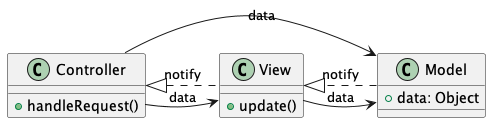
\includegraphics[width=0.8\textwidth]{fig/uml/default-mvc.png}
  \caption{Beispiel eines Basis MVC Architekturmusters}
  \label{fig:default-mvc}
\end{figure}

Diese Basisarchitektur wird nun in ein Fallbeispiel überführt, um verschiedene Aspkekte zu diskutieren. Das Szenario für die Fallstudie soll eine einfache Led-Lampe sein, die über eine eigene CPU und eigenen Speicher und einen Bluetooth Sender und Empfänger verfügt. Der Aufbau ist erweitert durch einen Raspberry PI, der sowohl die Anbindung der Lampe über Bluetooth repräsentiert, als auch den Servicezugriffspunkt für Applikationen im Internet. Der Raspberry Pi kann über eine Global Unicast IPv6 Adresse erreicht werden, um Steuerungssignale für die Lampe über die App abzugeben. 

Wir nutzen daher das Architekturmuster um eine Aufteilung in Verantwortlichkeiten zu realisieren. Jede Verantwortlichkeit - des PI, der Lampe und der Nutzerapp - wird in einer Klasse gekapselt. Die Zugehörigkeit zum MVC Pattern wird in diesem Beispiel dadurch Sterotypen zum Ausdruck gebracht.
\\\\
Eine Stereotype ist eine benutzerdefinierte Kennzeichnung eines UML-Elements, die durch das Hinzufügen von Namen, Attributen und Methoden definiert werden kann. Sie erweitern die UML-Notation und ermöglichen es, zusätzliche Informationen oder Bedeutungen einem Element zuzuweisen, ohne die zugrunde liegende UML-Syntax zu ändern. Stereotypen können auch dazu verwendet werden, bestimmte Funktionen oder Verhaltensweisen hinzuzufügen, die von der Basis-UML-Syntax nicht unterstützt werden. Zum Beispiel kann eine Stereotype \enquote{Singleton} einem Klassenobjekt hinzugefügt werden, um anzuzeigen, dass nur eine einzige Instanz dieser Klasse im gesamten System vorhanden sein sollte, oder wie in diesem Fall die Sterotype  \enquote{Model}. Mit Model wird die Klasse Lampe mit der Aufgabe des Buisnessmodells gebunden. 
Die Graphik~\ref{fig:stereo-mvc} zeigt das sich nun ergebene Bild. 
\begin{figure}[ht]
  \centering
  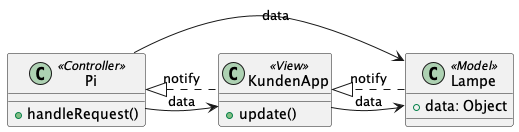
\includegraphics[width=0.8\textwidth]{fig/uml/sterotypen-mvc.png}
  \caption{MVC Architekturmusters im Fallbeispiel mit Sterotypen}
  \label{fig:stereo-mvc}
\end{figure}

Die Aufgaben der einzelnen Komponenten eines MVC-Architekturpatterns sind aber nicht trennscharf und sind wirklich einzig als ein \enquote{Best Practise} Beispiel anzusehen. Die folgende Aufzählung soll nur ein Einblick darin geben, wie weit die Aufgabenfelder der Komponenten erweitert werden können ohne das MVC-Architekturpattern zu verletzen. 
\begin{itemize}
\item Eine MVC-View kann neben ihrer Hauptfunktion, der Präsentation von Daten, auch weitere Aufgaben übernehmen. Sie kann beispielsweise automatisch die Darstellung von Daten anpassen, wenn Änderungen in den zugehörigen Modellen der Anwendung vorgenommen werden. Zudem kann sie Benutzeraktionen, die über grafische Eingabeelemente wie Textfelder oder Buttons erfolgen, an den Controller weiterleiten. Zusätzlich ist es möglich, dass die View Status- und Fehlermeldungen von Controllern visualisiert.

\item Ein MVC-Controller kann zusätzlich zu seiner Hauptaufgabe, der Steuerung des Datenflusses, weitere Funktionen übernehmen. Er kann beispielsweise Systemsignale wie eine Systemuhr verarbeiten und entsprechend darauf reagieren (z.B. Budget reicht nicht mehr für Nutzung). Zudem kann er die Komponentenlogik der Anwendung umsetzen und die Kommunikation mit externen Datenquellen für den Zweck der Datensynchronisation übernehmen.

\item Ein MVC-Modell kann neben der zentralen Verwaltung von Daten auch anderen Modulen Zugriff auf die Zustandsdaten gewähren und diese über Änderungen informieren, in der Regel mithilfe des Observer-Patterns. Zudem kann es die Komponentenlogik der Anwendung umsetzen und die Kommunikation mit externen Datenquellen koordinieren.
\end{itemize}

\subsubsection{VCM und CVM}
Das MVC Pattern selbst kann auch in unterschiedlichen Schichtenmodelle gedacht werden, die in ihrer Ausprägung beispielhaft VCM und CVM bezeichnet werden.  Es ist wichtig zu beachten, dass VCM und CVM keine weit verbreiteten oder standardisierten Architekturmuster sind, aber sie können als Variationen des MVC-Musters betrachtet werden, bei denen die Reihenfolge der Komponenten variiert und sich mit einem Schichtenmodell vereint. Die Graphik~\ref{fig:mvs-varianten} soll je Ausprägung eine mögliche Interpretation verdeutlichen.

\begin{figure}[ht]
  \centering
  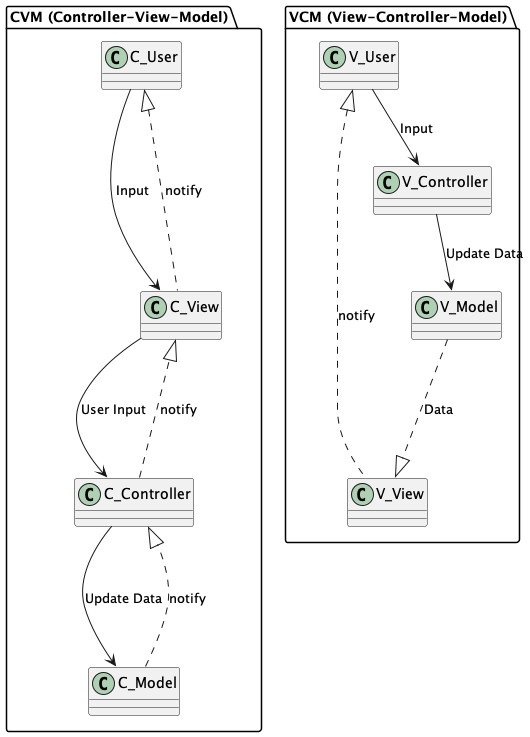
\includegraphics[width=0.65\textwidth]{fig/uml/mvc-varianten.png}
  \caption{Mögliche Varianten vom MVC in Schichten gedacht}
  \label{fig:mvs-varianten}
\end{figure}

Die drei Module einer Model-View-Controller (MVC)-Komponente sind gemäß dem Schichtenparadigma in Ebenen angeordnet. Die höheren Ebenen können auf die tiefergelegenen Ebenen zugreifen, aber nicht umgekehrt. Dies enspricht den Anforderungen an ein gerichtetes Schichtenmodel. 

Die unterste Ebene enthält das Modell. Das zugehörige Modul weiß nichts von den über ihm liegenden Modulen und kann mit diesen nur indirekt\footnote{zum Beispiel durch Antworten auf Nachrichten oder mit Hilfe eines sogenannten \enquote{handle} oder \enquote{callback}} kommunizieren.

Ein Controllermodul kann direkt auf ein Modellmodul zugreifen, um die Inhalte zu manipulieren. Eine View kommuniziert im Allgemeinen nur direkt mit Controllermodulen, um diesen Benutzeraktionen mitzuteilen.

In dem hier vorgestellten Szenario stellt der Benutzer das „oberste Modul“ dar. Er kommuniziert nur gerichtet mit View- und Controllermodulen. 

Wo die in diesem Beispiel aufgebaute CVM Struktur alle Schichten für den Weg zum Modell benutzt und mit dem handle über die Auswirkungen informiert, wird im Beispie des VCM Model für den Input die Schicht der View Klasse übersprungen, um eine direktere Eingabe zu unterstützen. Somit untstützt die VCM Struktur das MVC Muster, stützt das Schichtenmodell und eigenet sich auch für die Verarbeitung von zeitkritischen Inputs, wie sie beispielhaft in einem Jump'n'Run-Spiel gefordert sind. Nachteil es braucht direkte Kommunikationskanäle. Dieser direkte Weg ist aber nicht immer mögich, Technologien oder auch Frameworks verlangen bei User-Inputs nicht selten die klare Trennung von View und Kontroller. Ein Beispiel für solch eine technologische Anforderung wird von Java FX repräsentiert.     
\\\\
JavaFX ist ein relativ modernes Framework zur Erstellung von grafischen Benutzeroberflächen (GUIs) in Java. Es bietet verbesserte Möglichkeiten im Vergleich zu AWT und Swing. In JavaFX werden Benutzereingaben (User Inputs) über das Event-Handling-System verarbeitet. Hier ist ein Überblick darüber, wie JavaFX mit Benutzereingaben umgeht:
\begin{itemize}
\item Event-Handling: In JavaFX werden Ereignisse (Events) verwendet, um Benutzereingaben wie Mausklicks, Tastaturanschläge und andere Aktionen zu verarbeiten. Jedes Steuerelement (Control) oder Node in JavaFX kann Event-Handler registrieren, um auf spezifische Ereignisse zu reagieren.
\item Event-Typen: JavaFX bietet verschiedene Event-Klassen, die unterschiedliche Arten von Benutzereingaben repräsentieren, z. B. MouseEvent, KeyEvent, ScrollEvent usw. Sie können Event-Handler erstellen, die auf bestimmte Event-Typen reagieren, indem Sie die entsprechenden Methoden überschreiben.
\item Event-Handler: Um auf ein Ereignis zu reagieren, müssen Sie einen Event-Handler erstellen, der eine Methode handle() implementiert, die den Ereignistyp als Parameter akzeptiert. Sie können einen Event-Handler entweder als separate Klasse oder als Lambda-Ausdruck erstellen.
 \end{itemize}   

Das Code-Listing~\ref{lst:javafx-input} macht diese Anforderung dadurch deutlich, das die Java FX Anwendung die \enquote{javafx.application.Application} ableitet. In diesem Beispiel wird ein einfacher Button erstellt, der auf Mausklicks reagiert. Der Event-Handler wird mithilfe eines Lambda-Ausdrucks definiert und beim Klicken des Buttons wird \enquote{Button clicked!} in der Konsole ausgegeben. An dieser Stelle könnten die Daten vom Nutzer auch an den Kontroller weitergegeben werden.

\subsubsection{Vertreter}
Auch für die Verteilten Systeme machen die Schnittstellen und die Zuordnungen einen wichtigen unterschied. Jede Bindung der Komponenten bedarf einer Kommunikation, die im Zweifel mit einem Kommunktationsweg verbunden ist. Dieser Anforderung muss das Overlay- wie auch das physikalische Netzwerk entsprechen. Dies kann weitreichende Entscheidungen mit sich bringen. Stellen wir uns vor, das die Lampe in unserem Fallbeispiel über Bluetooth angesprochen werden muss, so ist aus der View kein direkter physikalischer Kommunikationsweg vorhanden, um einen handle zu nutzen ohne den Kontroller oder einen etwaigen Proxy einzusetzen.  Ein Proxy in einem verteilten System ist eine Komponente, die als Vermittler zwischen Clients und entfernten Diensten fungiert. Der Proxy ist eine Art Stellvertreter für den entfernten Dienst und ermöglicht es dem Client, auf diesen Dienst zuzugreifen, als ob er sich lokal im selben Netzwerk befände.
Der Proxy wird typischerweise zwischen dem Consumer und dem entfernten Dienst (Provider) platziert und übernimmt die Verwaltung der Kommunikation zwischen diesen beiden Komponenten. Der Client sendet Anfragen an den Proxy, der die Anfrage entgegennimmt und an den entfernten Dienst weiterleitet. Der entfernte Dienst sendet die Antwort an den Proxy zurück, der die Antwort an den Client weiterleitet.

\noindent\begin{minipage}{\textwidth}
\begin{lstlisting}[caption={Java FX Input},captionpos=b,label={lst:javafx-input}]
import javafx.application.Application;
import javafx.scene.Scene;
import javafx.scene.control.Button;
import javafx.scene.layout.StackPane;
import javafx.stage.Stage;

public class JavaFXUserInputExample extends Application {

    public static void main(String[] args) {
        launch(args);
    }

    @Override
    public void start(Stage primaryStage) {
        Button button = new Button("Click me!");

        // Registering an EventHandler for the button click
        button.setOnAction(event -> {
            System.out.println("Button clicked!");
        });

        StackPane root = new StackPane();
        root.getChildren().add(button);

        Scene scene = new Scene(root, 300, 250);

        primaryStage.setTitle("JavaFX User Input Example");
        primaryStage.setScene(scene);
        primaryStage.show();
    }
}
\end{lstlisting}
\end{minipage}

Ein Proxy bietet mehrere Vorteile in einem verteilten System. Zum Beispiel kann ein Proxy mit Caching dazu beitragen, die Netzwerklatenz zu reduzieren, indem er Anfragen von Clients bündelt und sie in einer einzigen Anfrage an den entfernten Dienst weiterleitet. Ein Proxy kann auch die Sicherheit erhöhen, indem er den Zugriff auf den entfernten Dienst kontrolliert und Anfragen von unautorisierten Clients blockiert. Das Diagramm \ref{fig:proxy} beschreibt die Idee als Muster von Komponenten:
\begin{figure}[ht]
  \centering
  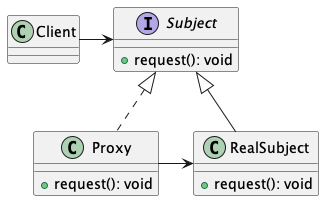
\includegraphics[width=0.45\textwidth]{fig/uml/proxy.png}
  \caption{Proxy Pattern}
  \label{fig:proxy}
\end{figure}
\begin{itemize}
\item Client: Die Klasse, die mit dem Subject-Interface interagiert.
\item  Subject: Das Interface, das von Proxy und RealSubject implementiert wird. Es definiert die gemeinsame Schnittstelle für Proxy und RealSubject.
\item RealSubject: Die Klasse, die das eigentliche Objekt repräsentiert, auf das der Proxy zugreifen soll.
\item Proxy: Die Klasse, die den Zugriff auf das RealSubject steuert.
\end{itemize}

Der Client interagiert mit dem Subject-Interface und kennt den Unterschied zwischen Proxy und RealSubject nicht. Der Proxy implementiert das Subject-Interface und steuert den Zugriff auf das RealSubject.

Es gibt verschiedene Arten von Proxies, die in einem verteilten System verwendet werden können, wie z.B. Forward Proxy, Reverse Proxy, Caching Proxy und Load Balancing Proxy. Jede Art von Proxy hat ihre eigenen Funktionen und Vorteile, je nach den Anforderungen des Systems und der Architektur.

\begin{itemize}
\item Ein Forward Proxy ist ein Proxy-Server, der als Vermittler zwischen einem Client und dem Internet fungiert. Wenn ein Client eine Anfrage an das Internet sendet, geht die Anfrage zuerst an den Forward Proxy-Server, der dann die Anfrage an das Ziel weiterleitet und die Antwort des Ziels an den Client zurücksendet.

Der Hauptzweck eines Forward Proxys besteht darin, die Privatsphäre und Sicherheit des Clients zu schützen, indem er seine Identität und IP-Adresse vor dem Zielserver verbirgt. Dadurch kann der Client anonym im Internet surfen und verhindern, dass die besuchten Websites seine IP-Adresse oder Identität aufzeichnen.

Forward Proxies werden auch oft in Unternehmen eingesetzt, um den Zugriff auf das Internet zu kontrollieren und zu beschränken. Sie können beispielsweise bestimmte Websites oder Dienste blockieren oder die Verwendung von bestimmten Protokollen einschränken.
\item Im Gegensatz zu einem Forward Proxy, der den Datenverkehr vom Client zu den Servern weiterleitet, empfängt ein Reverse Proxy Anfragen von den Servern und leitet sie an den Client weiter.

Der Hauptzweck eines Reverse Proxys besteht darin, die Last auf die Server zu verteilen, indem er eingehende Anfragen an verschiedene Server weiterleitet, um eine bessere Auslastung und Lastverteilung zu erreichen. Er kann auch zur Beschleunigung der Website-Leistung verwendet werden, indem er häufig angeforderte statische Inhalte im Cache speichert und schneller bereitstellt.

Reverse Proxies werden auch oft als Sicherheitsmaßnahme eingesetzt, um Angriffe auf die Server abzuwehren, indem sie den Server vor direktem Zugriff aus dem Internet schützen und nur autorisierte Anfragen durchlassen.

\item Ein Caching Proxy ist ein Proxy-Server, der den Datenverkehr zwischen einem Client und dem Internet überwacht und häufig abgerufene Inhalte im Cache speichert, um die Website-Leistung zu verbessern und die Belastung der Internetverbindung zu reduzieren.

Wenn ein Client eine Anfrage an das Internet sendet, überprüft der Caching Proxy, ob er eine Kopie der angeforderten Ressource im Cache hat. Wenn dies der Fall ist, wird die Ressource aus dem Cache geladen und an den Client zurückgesendet, ohne dass eine Verbindung zum ursprünglichen Server hergestellt werden muss. Wenn die Ressource nicht im Cache vorhanden ist, leitet der Caching-Proxy die Anfrage an den Server weiter und speichert dann die Antwort im Cache für zukünftige Anforderungen.

Caching-Proxies können dazu beitragen, die Leistung von Websites zu verbessern und die Latenzzeiten zu reduzieren, da häufig angeforderte Ressourcen schneller geladen werden können. Sie können auch dazu beitragen, die Bandbreitennutzung zu reduzieren, da der Proxy den Datenverkehr filtern und nur die notwendigen Ressourcen im Cache speichern kann.
\item Ein Load Balancing Proxy ist ein Proxy-Server, der als Vermittler zwischen einem Client und einem oder mehreren Servern fungiert und die Last auf mehrere Server verteilt, um eine bessere Auslastung und Verfügbarkeit zu erreichen.

Wenn ein Client eine Anfrage an den Load Balancing Proxy sendet, überprüft der Proxy die Server, die die Anfrage bearbeiten können, und leitet die Anfrage dann an den am wenigsten ausgelasteten Server weiter. Dadurch können mehrere Server gleichzeitig Anfragen bearbeiten, wodurch die Leistung und Verfügbarkeit der Anwendung verbessert werden.

Load Balancing Proxies sind besonders nützlich für Websites und Anwendungen mit hohem Traffic oder schweren Workloads, da sie dazu beitragen, die Belastung auf die Server zu reduzieren und eine hohe Verfügbarkeit sicherzustellen. Darüber hinaus können Load Balancing Proxies auch dazu beitragen, die Ausfallsicherheit zu verbessern, da im Falle eines Ausfalls eines Servers die Anfragen automatisch auf einen anderen Server umgeleitet werden können.
\end{itemize}
Ein Proxy ist normalerweise ein Vermittler, der  auf der Netzwerkebene arbeitet und als Gateway zwischen dem Client und dem Server fungiert. Eine Alternative Form zum Proxy kann auch als Broker beschrieben werden. 

Beide sind Vermittler, die in der Kommunikation zwischen verschiedenen Anwendungen verwendet werden. Der Hauptunterschied zwischen den beiden besteht darin, wie sie diese Kommunikation verarbeiten und welche Funktionen sie bereitstellen.

Ein Broker ist ein Vermittler, der die Kommunikation zwischen verschiedenen Anwendungen ermöglicht, indem er Nachrichten empfängt, speichert und an die richtigen Empfänger weiterleitet. Der Broker ist normalerweise in der Lage, die Nachrichten zu filtern, zu transformieren oder zu aggregieren, bevor er sie an den Empfänger weiterleitet. Der Broker kann auch verschiedene Messaging-Protokolle unterstützen und die Nachrichten in einer Warteschlange speichern, wenn der Empfänger nicht verfügbar ist. 

\begin{figure}[ht]
  \centering
  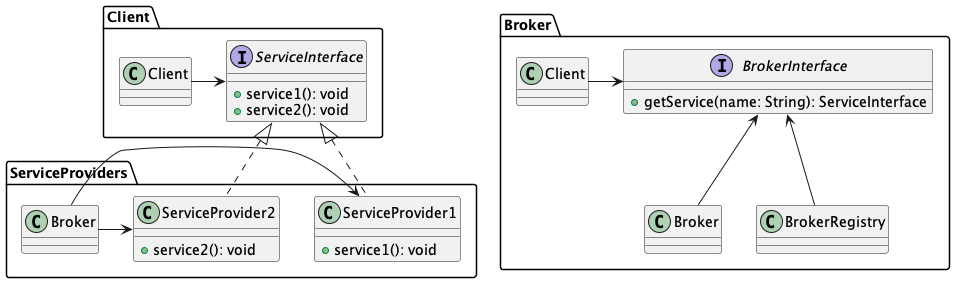
\includegraphics[width=0.95\textwidth]{fig/uml/broker.png}
  \caption{Broker Pattern}
  \label{fig:broker}
\end{figure}

Das Diagramm \ref{fig:broker} beschreibt das Broker-Pattern mit den folgenden Komponenten:
\begin{itemize}
\item Client: Die Klasse, die einen Dienst von einem der Service-Provider anfordert.
\item ServiceInterface: Das Interface, das von den ServiceProvidern implementiert wird. Es definiert die gemeinsame Schnittstelle für die angebotenen Dienste.
\item ServiceProvider1, ServiceProvider2: Die Klassen, die die tatsächlichen Dienste bereitstellen und das ServiceInterface implementieren.
\item BrokerInterface: Das Interface, das von Broker und BrokerRegistry implementiert wird. Es definiert die gemeinsame Schnittstelle, um auf die verschiedenen Dienste zuzugreifen.
\item Broker: Die Klasse, die als Vermittler zwischen Client und ServiceProvider fungiert und die Kommunikation vereinfacht.
\item BrokerRegistry: Die Klasse, die alle verfügbaren ServiceProvider verwaltet und dem Broker bei Bedarf zur Verfügung stellt.
\end{itemize}
Der Client greift über das BrokerInterface auf die gewünschten Dienste zu, ohne direkt mit den ServiceProvider-Klassen zu interagieren. Der Broker verwaltet die Kommunikation zwischen Client und ServiceProvider und entkoppelt so deren Abhängigkeiten.

Es ist weiter möglich eine weitere Unterschiedung in Forwarding-Broker und Handle-Driven-Broker einzuführen. 
Ein Forwarding-Broker ist ein Broker, der eingehende Nachrichten an den Empfänger weiterleitet, der von der Nachrichtadresse identifiziert wird. Der Broker hat keine Vorstellung von der Struktur oder dem Inhalt der Nachrichten, sondern dient lediglich als Vermittler zwischen Sender und Empfänger. Es handelt sich um ein sehr einfaches System, das schnell und effizient arbeitet, aber nur minimale Unterstützung für die Transformation von Nachrichten bietet.

Ein Handle-Driven-Broker ist dagegen ein Broker, der Nachrichten auf Basis eines Handles weiterleitet, das als Referenz auf eine Nachricht dient. Der Broker speichert den Handle und bietet verschiedene Funktionen an, um die Nachrichten zu bearbeiten oder zu transformieren, bevor sie an den Empfänger weitergeleitet werden. Handle-Driven-Broker bieten erweiterte Funktionen wie die Möglichkeit, Nachrichten zu filtern, zu transformieren oder zu aggregieren, bevor sie an den Empfänger weitergeleitet werden.

Auch der Broker kann im Funktionssatz nochmals in einem Trader erweitert werden. Ein Trader ist in einem verteilten System ein Teilnehmer, der versucht, bestimmte Dienste nach Regeln zu suchen oder anzubieten. Trader bieten eine Art von Gelbe Seiten für verteilte Dienste an, in denen sie Informationen wie Dienstbeschreibungen, Verfügbarkeit und Qualitätsmetriken speichern und veröffentlichen. Wenn ein Teilnehmer einen Dienst benötigt, sucht er nach einem passenden Trader und sucht dann nach einem geeigneten Dienst in den bereitgestellten Informationen. Als Pattern ist der Trader eher als Service Locator Pattern bekannt welches im Grundsatz aber sehr ähnlich zu dem Broker Pattern ist. 

Das wichtigste ist aber fernab aller Konnektivität die Umsetzung der handle, ob im direkten Zugriff oder über einen Vermittler. Für die Umsetzung von handle und für die Bindung von Schichten können unterschiedliche Ansätze genutzt werden, eine sehr verbreitete ist das Observer Pattern. 

\subsubsection{Observer Pattern}
In der Grundüberlegung des MVC ist das System eng gekoppelt und soll Änderungen im System immer unmittelbar signalisieren. Als Beispiel kann hier die Aktualisierung des Modells und die Implikation auf die View angesprochen werden. 
Wenn beispielhaft die Lampe angeschaltet wurde, soll das Ereignis auch unmittelbar auf der KundenApp angezeigt werden. 
Diese unmittelbare Kommunikation kann mit einem Observer-Pattern umgesetzt werden. 

Das Observer Pattern ist ein Entwurfsmuster, das verwendet wird, um eine 1:n-Beziehung zwischen Objekten zu erstellen, wobei Änderungen an einem Objekt automatisch an andere Objekte weitergegeben werden. Das bedeutet, dass ein Objekt (das sogenannte Subjekt) alle seine Beobachter (die Observer) benachrichtigt, wenn sich sein Zustand ändert. Die Beobachter reagieren dann auf diese Änderung entsprechend.

Das Observer Pattern wird oft in Situationen eingesetzt, in denen es wichtig ist, dass eine Änderung an einem Objekt die darauf basierenden Objekte informiert und automatisch aktualisiert. Zum Beispiel kann ein Nachrichtendienst ein Subjekt sein, das Nachrichten an viele Abonnenten weiterleitet. Ein weiteres Beispiel wäre ein Diagramm, das automatisch aktualisiert wird, wenn sich die zugrunde liegenden Daten ändern.

Das Observer Pattern besteht aus einem Subjekt, das eine Liste von Beobachtern hält, sowie einer Schnittstelle, die es Beobachtern ermöglicht, auf Änderungen zu reagieren. Wenn sich der Zustand des Subjekts ändert, wird diese Änderung an alle Beobachter übermittelt. Die Beobachter können dann auf diese Änderung reagieren und ihre eigenen Aktionen durchführen.
\begin{figure}[ht]
  \centering
  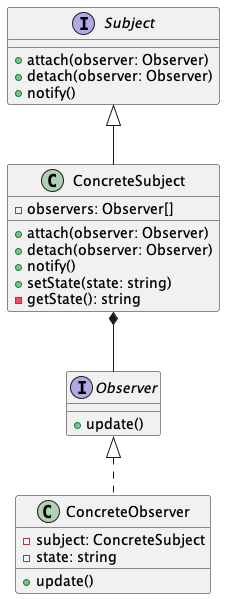
\includegraphics[width=0.25\textwidth]{fig/uml/default-observer.png}
  \caption{Einfaches Observer Pattern}
  \label{fig:default-observer}
\end{figure}

Das Observer Pattern ermöglicht eine flexible und erweiterbare Architektur, da Subjekte und Beobachter unabhängig voneinander implementiert werden können. Subjekte können Beobachter hinzufügen oder entfernen, ohne dass dies Auswirkungen auf den Rest des Systems hat. Beobachter können ebenfalls hinzugefügt oder entfernt werden, ohne dass Änderungen an anderen Teilen des Systems vorgenommen werden müssen.

Die Graphik~\ref{fig:default-observer} zeigt das Observer Pattern mit drei Komponenten: Subject, Observer und ConcreteSubject. Das Subject ist eine Schnittstelle, die von den Subjekten implementiert wird, die beobachtet werden sollen. Es definiert Methoden zum Hinzufügen, Entfernen und Benachrichtigen von Beobachtern. Der Observer ist eine Schnittstelle, die von allen Beobachtern implementiert wird, und definiert eine Methode zum Aktualisieren des Beobachters, wenn sich der Zustand des Subjekts ändert.

Der ConcreteSubject ist das Subjekt, das beobachtet werden soll. Es hält eine Liste von Beobachtern und implementiert die Methoden zum Hinzufügen, Entfernen und Benachrichtigen von Beobachtern. Der ConcreteObserver ist ein Beobachter, der den Zustand des Subjekts aktualisiert, wenn sich dieser ändert.
\\\\
Das Observer Pattern ermöglicht eine lose Kopplung zwischen Subjekten und Beobachtern, da Subjekte nicht von spezifischen Beobachtern abhängig sind und Beobachter nicht von spezifischen Subjekten. Man beachte das eine lose Kopplung zwischen den Komponenten gelingt, aber eine enge Kopplung bei der Kommunikation unterstützt wird. 

Für unser Anwendungsbeispiel angepasst, soll das Oberver-Pattern zwischen der KundenApp (View) und der Lampe (Model) etabliert werden. Eine vereinfachte Architektur könnte wie in Graphik~\ref{fig:mvc-observer} aufgebaut werden. 

\begin{figure}[ht]
  \centering
  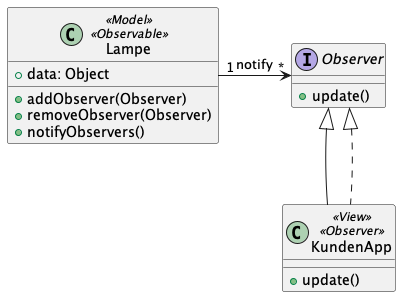
\includegraphics[width=0.45\textwidth]{fig/uml/mvc-observer.png}
  \caption{Observer Pattern als Verbindung zwischen Model und View}
  \label{fig:mvc-observer}
\end{figure}

Natürlich ist ein Architektur-Modell nicht ausreichend um das gesamte Design zu beschreiben, das MVC Architektur-Modell braucht weitere Informationen für das vollständige System. Eine wichtige zusätliche Information ist das Verhalten der Architektur. Auch für dieses Verhalten bestehen \enquote{Best Practise} Ansätze, die wir als Verhaltensmuster (Behavioral Patterns) beschreiben. 

Verhaltensmuster genannt, sind Entwurfsmuster in der Softwareentwicklung, die sich mit der Organisation und Steuerung von Objekten und deren Interaktionen beschäftigen. Sie beschreiben, wie verschiedene Objekte zusammenarbeiten und wie sie Verhaltensweisen und Aufgaben koordinieren.

Behavioral Patterns beschreiben das Verhalten von Objekten in bestimmten Situationen und stellen somit Lösungen für wiederkehrende Probleme bereit, wie z.B. die Steuerung von Abläufen, die Verwaltung von Zuständen oder die Behandlung von Fehlern. Es gibt verschiedene Arten von Behavioral Patterns, die je nach Art der Aufgabe, die sie lösen sollen, in verschiedene Kategorien unterteilt werden können:
\begin{itemize}
\item Klassifizierungsmuster (Classification Patterns): Diese Muster beschreiben, wie Objekte in Klassen und Kategorien organisiert werden können, um eine effektive Klassifizierung und Strukturierung von Objekten zu ermöglichen. Ein Beispiel für ein solches Muster ist das Strategy Pattern.
\item Kommunikationsmuster (Communication Patterns): Diese Muster beschreiben, wie Objekte miteinander kommunizieren und wie Nachrichten oder Daten zwischen ihnen ausgetauscht werden können. Ein Beispiel für ein solches Muster ist das Observer Pattern.
\item Kontrollmuster (Control Patterns): Diese Muster beschreiben, wie Objekte kontrolliert und gesteuert werden können, um eine effektive Durchführung von Abläufen und Prozessen zu ermöglichen. Ein Beispiel für ein solches Muster ist das Command Pattern.
\item Datenmuster (Data Patterns): Diese Muster beschreiben, wie Daten zwischen Objekten ausgetauscht und gespeichert werden können. Ein Beispiel für ein solches Muster ist das Iterator Pattern.
\end{itemize}
Es ergibt sich natürlich das die Kommunikationsmuster eine besondere Bedeutung in dem Design eines verteilten Systems einnehmen. 
\\\\
Für die Beschreibung von Behavioral Patterns eignen sich in UML (Unified Modeling Language) vor allem die folgenden Diagrammtypen:
\begin{itemize}
\item Aktivitätsdiagramme (Activity Diagrams): Diese Diagramme werden verwendet, um die Abläufe und Prozesse in einem System oder einer Anwendung zu beschreiben. Aktivitätsdiagramme können verwendet werden, um die Interaktionen zwischen verschiedenen Objekten in einem Behavioral Pattern darzustellen.
\item Sequenzdiagramme (Sequence Diagrams): Diese Diagramme werden verwendet, um die Interaktionen zwischen verschiedenen Objekten in einer bestimmten Sequenz darzustellen. Sequenzdiagramme können verwendet werden, um die Kommunikationsmuster in einem Behavioral Pattern zu beschreiben.
\item Zustandsdiagramme (State Diagrams): Diese Diagramme werden verwendet, um den Zustand eines Objekts und die Übergänge zwischen verschiedenen Zuständen zu beschreiben. Zustandsdiagramme können verwendet werden, um die Kontrollmuster in einem Behavioral Pattern zu beschreiben.
\item Interaktionsübersichtsdiagramme (Interaction Overview Diagrams): Diese Diagramme werden verwendet, um die Interaktionen zwischen verschiedenen Objekten und deren Kommunikationsmuster in einem System oder einer Anwendung zu beschreiben. Interaktionsübersichtsdiagramme können verwendet werden, um eine Übersicht über die Interaktionen in einem Behavioral Pattern zu geben.
\end{itemize}
Durch die Verwendung dieser Diagrammtypen können Behavioral Patterns effektiv beschrieben und visualisiert werden, was zu einer verbesserten Verständlichkeit und Kommunikation der Konzepte und Strukturen innerhalb des Patterns führt.
\\\\
In dem Fallbeispiel der Lampe soll zur Verdeutlichung die einfache Sequenz des Hinzufügen eines Observers zwischen PI (Controller) und Lampe (Model) den Nutzen verdeutlichen. 

\begin{figure}[ht]
  \centering
  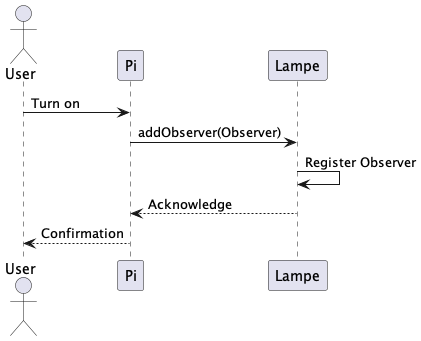
\includegraphics[width=0.55\textwidth]{fig/uml/seq-mvc-observer.png}
  \caption{Observer Pattern als Verbindung zwischen Model und View}
  \label{fig:seq-mvc-observer}
\end{figure}

Im Sequenzdiagramm~\ref{fig:seq-mvc-observer} sind die Schritte zum Hinzufügen eines Observers wie folgt beschrieben:
\begin{itemize}
\item Der Benutzer initiiert den Prozess, indem er den Controller bittet, einen neuen Observer hinzuzufügen.
\item Der Controller ruft die \enquote{addObserver()} Methode des Models auf und übergibt den Observer als Parameter.
\item Das Model registriert den neuen Observer intern, z.B. indem es ihn in einer Liste von Beobachtern speichert.
\item Nachdem der Observer erfolgreich registriert wurde, bestätigt das Model dies dem Controller.
\item Schließlich bestätigt der Controller dem Benutzer, dass der Observer erfolgreich hinzugefügt wurde.
\end{itemize}
Dieses Sequenzdiagramm zeigt die Interaktionen zwischen Benutzer, Controller, Model und Observer beim Hinzufügen eines Observers im Kontext eines MVC-Architekturmusters bei der Initialisierung des Systems. Es ist sicherlich schnell zu erkennen, das weder das Behavioral Pattern noch das Architecture Pattern alleine ausreichend Informationen bietet. Nur in gegenseitiger Ergänzung bieten sie ein vollständiges Bild. Dem geneigten Leser ist es in diesem Fall als Übung überlassen, die Architektur mit dem Observer zwischen Pi und Lampe zu beschreiben, wie das Verhalten an der Schnittstelle Lampe und KundenAPP. 
\\\\
Ob das MVC-Pattern mit einer Kopplung über das Observer Pattern gelingt, ist nicht nur eine Design, sondern auch eine Technologie-abhängige Fragestellung. Das Observer Pattern verlangt die Möglichkeit einer unabhängigen uni-direktionalen Kommunikation zwischen dem Subjekt und den Beobachtern, die nur in eine Richtung erfolgt. Dies ist sowohl in einem Programmstack möglich, als auch bei der klassischen Socket-Kommunikation. Beispielhaft ist TCP ein Transportprotokoll auf Layer 4 des ISO-OSI Refernezmodells, welches als Schnittstelle über die Socket-API den Entwicklern bereitgestellt wird. Mit einem Applikations-Protokoll, das diese Eigenschaften nutzt, ist eine Umsetzung des Observer-Patterns eine gute Wahl. 
\\\\
In klassischen Web-Applikationen, selbst wenn sie auf UDP oder TCP basieren, ist dies ohne weiteres nicht der Fall. Als Beispiel kann das HTTP Protokoll herangezogen werden, das auf Basis von TCP ein zustandloses Protokoll anbietet und zudem dem Request-Response-Cycle unterliegt. Insbesondere der Request-Response-Cycle setzt für jede Anfrage eine Antwort voraus und wiederspricht der Funktionsweise des Observer Patterns.
\\\\
In der Praxis können Techniken wie WebSockets oder Long Polling verwendet werden, um eine Art Zustand und damit unahbängige Kommunikation zwischen Subjekt und den Beobachtern zu simulieren und das Observer-Pattern zu verwenden, dennoch sind diese Lösungen nicht Teil von älteren HTTP Standards und in Teilen sehr Fehler-anfällig. Zur Erklärung, bei diesen Lösungen werden Verbindungen zwischen Subjekt und den Beobachter aufrechterhalten und bei Zustandsänderungen werden die entsprechenden Beobachter benachrichtigt. Allerdings sind diese Techniken mit erhöhtem Aufwand verbunden und haben auch andere Nachteile, wie z.B. eine höhere Netzwerklast und eine höhere Komplexität in der Implementierung. 
Auch werden in unterschiedlichen HTTP Versionen unterschiedlichen \enquote{Workarounds} angeboten. So können bei HTTP2/ HTTP3 Technologien wie Server-Push Mechanismen genutzt werden, sie werden aber stark im Kontext der Sicherheit diskutiert. 
\\\\
Neben dem Observer Pattern, sieht man in Verteilten Systemen auch immer wieder das Callback Pattern eingesetzt, da es nur einfachere Kommunikationsstrukturen braucht. In Situationen, in denen nur eine einzige Funktion oder ein einziges Objekt auf ein bestimmtes Ereignis reagieren muss, bietet daher das Callback-Pattern eine einfachere und leichter verständliche Implementierung.

Das Callback-Pattern ist auch nützlich, wenn es darum geht, den Programmfluss nicht zu blockieren, insbesondere bei asynchronen oder zeitintensiven Operationen. Es ermöglicht die Ausführung anderer Aufgaben, während die lang andauernde Operation im Hintergrund abläuft, und die Callback-Funktion wird aufgerufen, sobald die Operation abgeschlossen ist.

\subsubsection{Callback Pattern}
Das Callback-Pattern ist ein Verhaltensmuster in der Softwareentwicklung, bei dem eine Funktion (auch als Methode oder Prozedur bezeichnet) als Argument an eine andere Funktion übergeben wird. Diese übergebene Funktion, die als Callback-Funktion bezeichnet wird, wird zu einem späteren Zeitpunkt, oft nach Abschluss einer bestimmten Aufgabe oder einem Ereignis, vom aufrufenden Code ausgeführt. Das Callback-Pattern wird häufig verwendet, um asynchrone Programmierung, Ereignisbehandlung oder die Entkopplung von Funktionen zu ermöglichen.

\begin{figure}[!ht]
  \centering
  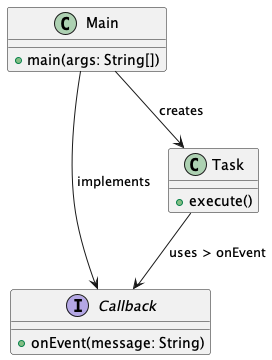
\includegraphics[width=0.30\textwidth]{fig/uml/callback-class.png}
  \caption{Callback Pattern}
  \label{fig:callback-class}
\end{figure}

Hier ist eine Beschreibung der Schlüsselelemente des Callback-Patterns:
\begin{itemize}
\item Funktion als Parameter: Im Callback-Pattern wird eine Funktion als Argument an eine andere Funktion übergeben. Die übergebene Funktion ist die Callback-Funktion.
\item Rückrufzeitpunkt: Die Callback-Funktion wird zu einem bestimmten Zeitpunkt aufgerufen, beispielsweise nach Abschluss einer Aufgabe oder beim Eintreten eines Ereignisses. Der Zeitpunkt, wann die Callback-Funktion aufgerufen wird, kann variieren und hängt von der Implementierung und den Anforderungen der Anwendung ab.
\item Entkopplung: Durch die Verwendung des Callback-Patterns können zwei Funktionen entkoppelt werden. Das bedeutet, dass die aufrufende Funktion nicht wissen muss, wie die Callback-Funktion implementiert ist, solange sie das erwartete Verhalten aufweist.
\item Einfachheit: Das Callback-Pattern ist für einfache Kommunikationsanforderungen zwischen Funktionen oder Objekten geeignet. Es ist besonders nützlich, wenn es nur eine geringe Anzahl von beteiligten Funktionen oder Objekten gibt und die Kommunikation unidirektional ist.
\item Asynchrone Programmierung: Das Callback-Pattern wird häufig in der asynchronen Programmierung verwendet, um den Programmfluss nicht zu blockieren. Wenn eine zeitintensive Operation ausgeführt wird, kann die Callback-Funktion bei Abschluss dieser Operation aufgerufen werden, sodass der restliche Code ohne Verzögerung weiterlaufen kann.
\item Ereignisgesteuert: Das Callback-Pattern eignet sich gut für ereignisgesteuerte Programmierung, bei der bestimmte Aktionen aufgrund von Ereignissen oder Benutzerinteraktionen ausgeführt werden sollen. Die Callback-Funktionen dienen als Reaktionen auf diese Ereignisse und werden ausgeführt, wenn das Ereignis eintritt.
\end{itemize}

\begin{figure}[!ht]
  \centering
  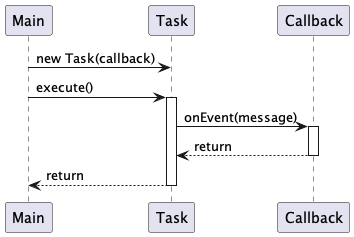
\includegraphics[width=0.50\textwidth]{fig/uml/callback-seq.png}
  \caption{Callback Pattern Sequenz}
  \label{fig:callback-seq}
\end{figure}

In dem Diagrammen ~\ref{fig:callback-class} und ~\ref{fig:callback-seq} wird das Callback-Pattern über die Callback-Schnittstelle, die Task-Klasse und die Main-Klasse dargestellt. Die Callback-Schnittstelle definiert die Methode onEvent(), die später als Callback-Funktion verwendet wird. Die Task-Klasse enthält die execute()-Methode, die die Callback-Funktion aufruft, wenn eine bestimmte Aktion oder ein bestimmtes Ereignis eintritt. Schließlich erstellt die Main-Klasse sowohl ein Task-Objekt als auch eine Implementierung der Callback-Schnittstelle und stellt die Kommunikation zwischen diesen beiden Elementen her.
\\\\
Obwohl Callback Pattern und Observer Pattern beide Techniken zur Implementierung von ereignisgesteuerten Kommunikationen zwischen Objekten sind, gibt es einige wichtige Unterschiede zwischen ihnen.

\begin{itemize}
\item Im Callback Pattern wird eine Funktion (Callback-Funktion) als Parameter an ein anderes Objekt oder eine Funktion übergeben.
\item Die aufgerufene Funktion oder das aufgerufene Objekt führt die übergebene Callback-Funktion unter bestimmten Bedingungen aus (z.B. nachdem eine bestimmte Aktion abgeschlossen ist).
\item Das Callback Pattern ermöglicht eine einfache, unidirektionale Kommunikation zwischen zwei Objekten oder Funktionen.
\item Das Callback Pattern eignet sich gut für einfache und direkte Kommunikationsanforderungen, bei denen nur eine geringe Anzahl von Funktionen oder Objekten beteiligt ist.
\end{itemize}



\noindent\begin{minipage}{\textwidth}
\begin{lstlisting}[caption={Callback Pattern},captionpos=b,label={lst:callback}]
// Callback-Interface
interface Callback {
    void onEvent(String message);
}

// Klasse, die die Callback-Funktion verwendet
class Task {
    private Callback callback;

    public Task(Callback callback) {
        this.callback = callback;
    }

    public void execute() {
        // ... fuehre einige Aktionen aus
        callback.onEvent("Task abgeschlossen");
    }
}

// Hauptklasse
public class Main {
    public static void main(String[] args) {
        Callback callback = message -> System.out.println("Callback erhalten: " + message);
        Task task = new Task(callback);
        task.execute();
    }
}
\end{lstlisting}
\end{minipage}

\begin{itemize}
\item Im Observer Pattern (auch bekannt als \enquote{Publish-Subscribe Pattern}) gibt es ein \enquote{Subject} (oder \enquote{Publisher}) und mehrere \enquote{Observer} (oder \enquote{Subscriber}).
\item Die Observer registrieren sich beim Subject, um über Änderungen oder Ereignisse informiert zu werden.
\item Wenn ein Ereignis beim Subject eintritt, benachrichtigt es alle registrierten Observer, indem es eine spezielle Methode in den Observer-Objekten aufruft.
\item Das Observer Pattern ermöglicht eine lose Kopplung zwischen Objekten und ist skalierbar, da eine beliebige Anzahl von Observern benachrichtigt werden kann, ohne dass das Subject deren Implementierung
\end{itemize}

\noindent\begin{minipage}{\textwidth}
\begin{lstlisting}[caption={Observer Pattern - ConcreteSubject},captionpos=b,label={lst:observer-I}]
import java.util.ArrayList;
import java.util.List;

// Subject-Interface
interface Subject {
    void addObserver(Observer observer);
    void removeObserver(Observer observer);
    void notifyObservers();
}

// Observer-Interface
interface Observer {
    void update(String message);
}

// ConcreteSubject
class Task implements Subject {
    private List<Observer> observers = new ArrayList<>();
    private String message;

    public void execute() {
        // ... fuehre einige Aktionen aus
        message = "Task abgeschlossen";
        notifyObservers();
    }

    @Override
    public void addObserver(Observer observer) {
        observers.add(observer);
    }

    @Override
    public void removeObserver(Observer observer) {
        observers.remove(observer);
    }

    @Override
    public void notifyObservers() {
        for (Observer observer : observers) {
                     observer.update(message);
        }
    }
}


\end{lstlisting}
\end{minipage}

\noindent\begin{minipage}{\textwidth}
\begin{lstlisting}[caption={Observer Pattern - Concrete Observer},captionpos=b,label={lst:observer-II}]
// ConcreteObserver
class TaskObserver implements Observer {
    private String observerName;

    public TaskObserver(String observerName) {
        this.observerName = observerName;
    }

    @Override
    public void update(String message) {
        System.out.println(observerName + " hat eine Benachrichtigung erhalten: " + message);
    }
}

// Hauptklasse
public class Main {
    public static void main(String[] args) {
        Task task = new Task();
        TaskObserver observer1 = new TaskObserver("Observer1");
        TaskObserver observer2 = new TaskObserver("Observer2");

        task.addObserver(observer1);
        task.addObserver(observer2);

        task.execute();

        task.removeObserver(observer1);

        task.execute();
    }
}
\end{lstlisting}
\end{minipage}

Im Listing~\ref{lst:callback} und Listing~\ref{lst:observer-I},~\ref{lst:observer-II} ist zu sehen, wie das Callback Pattern und das Observer Pattern in Java-Code implementiert werden. Im Callback Pattern wird eine Funktion direkt an die ausführende Klasse (Task) übergeben, während im Observer Pattern die Observer sich beim Subject (auch Task in diesem Beispiel) registrieren, um Benachrichtigungen zu erhalten.

Für Verteilte Systeme ist sowohl für das Observer Pattern als auch das Callback Pattern die Referenzen des Callbacks bzw. des Observers eine Herausforderung. Da Verteilte Systeme sich keinen gemeinsamen Speicher teilen, muss ein Ersatz für die Adressierung der Referenz gefunden werden, dies soll zu einem späteren Zeitpunkt diskutiert werden. 

Wenn die fehlende Adressierung gelöst ist, sollte insgesamt das Callback-Pattern in Betracht gezogen werden, wenn die Anforderungen an die Kommunikation zwischen den beteiligten Funktionen oder Objekten weniger komplex sind und eine einfachere, unidirektionale Kommunikation ausreicht. Wenn jedoch mehrere Objekte auf das gleiche Ereignis reagieren müssen oder eine losere Kopplung zwischen den beteiligten Objekten erforderlich ist, ist das Observer-Pattern besser geeignet.

Neben der Kommunikation der Komponenten die zudem noch in eine Uni- oder Mulitcast Kommunikation unterschieden werden kann, muss auch die Initialisierung für verteilte Systeme diskutiert werden. In diesem Script sollen neben den Singleton und den Factory Pattern auch die Initialisierung mit Dependency Injection besprochen werden.

\subsubsection{Singleton Pattern}

Das Singleton-Pattern ist ein Entwurfsmuster, das sicherstellt, dass eine Klasse nur eine einzige Instanz hat und einen globalen Zugriffspunkt zu dieser Instanz bereitstellt. In verteilten Systemen kann die Verwendung des Singleton-Patterns einige Herausforderungen mit sich bringen, da es mehrere Knoten oder Prozesse gibt, die möglicherweise auf die Singleton-Instanz zugreifen müssen.
\begin{figure}[!ht]
  \centering
  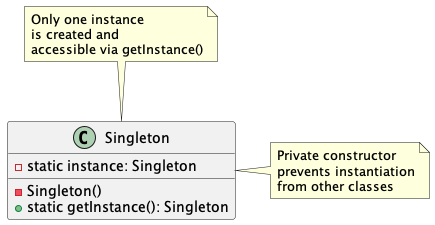
\includegraphics[width=0.45\textwidth]{fig/uml/singleton.png}
  \caption{Singleton Pattern}
  \label{fig:singleton}
\end{figure}

In dem Diagramm~\ref{fig:singleton} gibt es eine Singleton-Klasse, die das Singleton-Pattern implementiert. Die Klasse hat:
\begin{itemize}
\item Eine private statische Variable instance, die die einzige Instanz der Singleton-Klasse speichert.
\item Einen privaten Konstruktor (Singleton()), der die Erstellung von Instanzen der Singleton-Klasse von außen verhindert.
\item Eine öffentliche statische Methode getInstance(), die die einzige Instanz der Singleton-Klasse zurückgibt oder bei Bedarf erstellt.
\end{itemize}
Die Anmerkungen im Diagramm verdeutlichen, dass der private Konstruktor die Instanziierung von anderen Klassen verhindert und dass nur eine Instanz der Singleton-Klasse erstellt und über die getInstance()-Methode zugänglich gemacht wird.
\begin{itemize}
\item Ressourcenverwaltung: Das Singleton-Pattern kann bei der Verwaltung von Ressourcen, wie zum Beispiel Verbindungen zu Datenbanken oder Diensten, nützlich sein. Es kann dazu beitragen, den Ressourcenverbrauch zu minimieren, indem es verhindert, dass mehrere Verbindungen oder Instanzen erstellt werden, die dieselben Ressourcen verwenden.
\item Zentrale Steuerung: Ein Singleton kann als zentrale Steuerungs- oder Koordinationskomponente in einem verteilten System dienen, indem es sicherstellt, dass es nur eine einzige Instanz gibt, die den globalen Zustand verwaltet.
\end{itemize}
\begin{itemize}
\item Skalierbarkeit: Das Singleton-Pattern kann die Skalierbarkeit eines verteilten Systems beeinträchtigen, da alle Knoten oder Prozesse auf die einzelne Instanz des Singleton-Objekts zugreifen müssen. Dadurch kann es zu Engpässen oder Leistungsproblemen kommen, wenn die Anzahl der Knoten oder Prozesse zunimmt.
\item Synchronisation: In verteilten Systemen kann die Synchronisation von Singleton-Instanzen eine Herausforderung darstellen. Um sicherzustellen, dass alle Knoten dieselbe Singleton-Instanz verwenden, muss ein Mechanismus implementiert werden, um den globalen Zustand der Instanz konsistent zu halten. Dies kann zusätzliche Komplexität und Overhead verursachen, insbesondere wenn das verteilte System auch fehlertolerant sein muss.
\item Fehlertoleranz: Ein Singleton-Objekt kann in einem verteilten System zu einem Single Point of Failure (SPOF) werden. Wenn die Singleton-Instanz ausfällt, kann dies das gesamte System beeinträchtigen. Um dieses Problem zu umgehen, sind zusätzliche Maßnahmen wie Replikation oder Clustering erforderlich, die die Komplexität erhöhen und möglicherweise die Vorteile des Singleton-Patterns zunichte machen.
\end{itemize}
Die Eignung des Singleton-Patterns hängt in verteilten Systemen von den spezifischen Anforderungen und der Architektur des Systems ab. In einigen Fällen kann das Singleton-Pattern Vorteile bieten, wie das zentrale Verwalten von Ressourcen und die Steuerung des globalen Zustands. In anderen Fällen können die Nachteile, wie eingeschränkte Skalierbarkeit, Synchronisationsprobleme und die Notwendigkeit, Fehlertoleranz zu gewährleisten, dazu führen, dass das Singleton-Pattern für verteilte Systeme weniger geeignet ist.

\subsubsection{Factory Pattern}
Das Factory-Pattern ist ein Entwurfsmuster, das Objekterstellung auf eine separate Factory-Klasse auslagert. Dies ermöglicht die Erstellung von Objekten, ohne dass der Client-Code direkt den Konstruktor der Objekte aufrufen muss. In verteilten Systemen kann das Factory-Pattern einige Vorteile bieten:
\begin{itemize}
\item Abstraktion und Entkopplung: Das Factory-Pattern hilft, den Client-Code von den konkreten Implementierungsdetails der erstellten Objekte zu entkoppeln. In verteilten Systemen kann dies besonders nützlich sein, da Änderungen an den Implementierungen von Diensten oder Komponenten ohne Auswirkungen auf den Client-Code vorgenommen werden können. Dies erleichtert die Wartung und Skalierung des Systems.
\item Flexibilität bei der Objekterstellung: Das Factory-Pattern ermöglicht es, verschiedene Implementierungen von Objekten zu erstellen, basierend auf der Systemkonfiguration oder den Anforderungen des verteilten Systems. Dies kann dazu beitragen, dass das System einfacher an unterschiedliche Umgebungen oder Anforderungen angepasst werden kann.
\item Vereinfachung der Objekterstellung: In verteilten Systemen kann die Erstellung von Objekten, insbesondere von Ressourcen wie Verbindungen zu Datenbanken oder externen Diensten, komplex sein. Das Factory-Pattern kann dazu beitragen, diese Komplexität zu kapseln und die Erstellung von Objekekten für den Client-Code zu vereinfachen. Dadurch wird der Code leichter verständlich und wartbar.
\item Zentrale Verwaltung von Ressourcen: In verteilten Systemen kann die Verwaltung von Ressourcen wie Verbindungen oder Diensten eine Herausforderung darstellen. Durch die Verwendung des Factory-Patterns können diese Ressourcen zentral erstellt und verwaltet werden, was zu einer besseren Kontrolle und einem effizienteren Ressourcenmanagement führt.
\item Load Balancing und Failover: Das Factory-Pattern kann in verteilten Systemen dazu verwendet werden, Load Balancing und Failover-Mechanismen zu implementieren. Die Factory kann die Anfragen auf verschiedene Knoten oder Instanzen verteilen, um die Last auszugleichen oder im Falle eines Ausfalls auf einen anderen Knoten umzuschalten. Dies trägt zur Skalierbarkeit und Fehlertoleranz des Systems bei.
\end{itemize}
\begin{figure}[!ht]
  \centering
  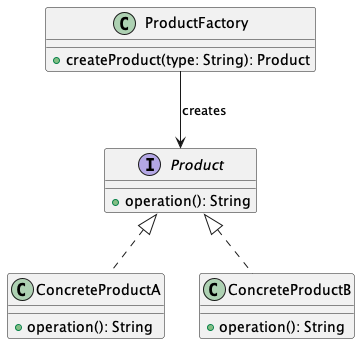
\includegraphics[width=0.45\textwidth]{fig/uml/factory-class.png}
  \caption{Factory Pattern}
  \label{fig:factory-class}
\end{figure}
Das Diagramm~\ref{fig:factory-class} beschreibt das Factory Pattern.
\begin{itemize}
\item Ein Product-Interface, das die gemeinsame Schnittstelle für alle Produkte definiert.
\item Zwei konkrete Produktklassen (ConcreteProductA und ConcreteProductB), die das Product-Interface implementieren. Sie stellen unterschiedliche Produktvarianten dar.
\item Eine ProductFactory-Klasse, die für die Erstellung von Product-Objekten verantwortlich ist.
\end{itemize}
Das Factory-Pattern kapselt die Logik zur Erstellung von Produktobjekten in der ProductFactory-Klasse. Der Client-Code verwendet die createProduct()-Methode der Factory, um ein Produktobjekt zu erstellen, ohne sich um die konkreten Implementierungsdetails der Produktklassen kümmern zu müssen. Das Diagramm zeigt, dass die ProductFactory-Klasse das Product-Interface verwendet, um Produktobjekte zu erstellen, wobei die konkreten Produktklassen die Implementierung bereitstellen.

\begin{figure}[!ht]
  \centering
  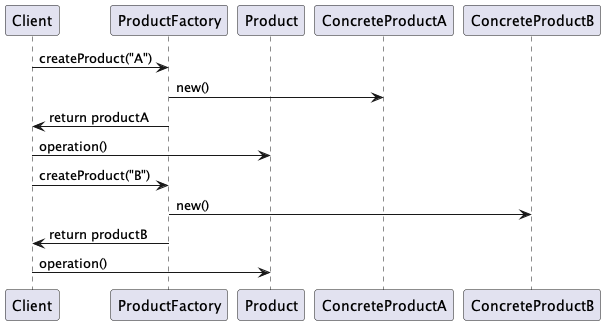
\includegraphics[width=0.85\textwidth]{fig/uml/factory-seq.png}
  \caption{Factory Pattern Sequenz}
  \label{fig:factory-seq}
\end{figure}

Insgesamt bietet das Factory-Pattern in verteilten Systemen eine Reihe von Vorteilen, die dazu beitragen, den Code sauberer und wartbarer zu gestalten, die Skalierbarkeit und Fehlertoleranz zu verbessern und die Verwaltung von Ressourcen zu optimieren. Durch die Abstraktion der Objekterstellung und die zentrale Verwaltung von Ressourcen trägt das Factory-Pattern zur Effizienz und Flexibilität in verteilten Systemen bei.

Obwohl das Factory-Pattern in vielen verteilten Systemen Vorteile bietet, gibt es auch Situationen, in denen Probleme auftreten können:
\begin{itemize}
\item Kommunikationslatenz: In verteilten Systemen kann die Kommunikation zwischen den Knoten und den Factory-Instanzen Latenz verursachen. Wenn der Factory-Code auf einem zentralen Knoten gehostet wird, kann dies zu Verzögerungen bei der Objekterstellung führen und die Gesamtleistung des Systems beeinträchtigen.
\item Synchronisation: In verteilten Systemen kann die Synchronisation der Factory-Instanzen über mehrere Knoten hinweg eine Herausforderung darstellen. Wenn der Factory-Code oder die Konfigurationsinformationen geändert werden, müssen alle Factory-Instanzen im System aktualisiert werden, um konsistent zu bleiben. Dies kann zu zusätzlicher Komplexität und möglichen Inkonsistenzen führen.
\item Single Point of Failure (SPOF): Wenn die Factory zentral verwaltet wird oder auf einem einzelnen Knoten gehostet ist, kann dies zu einem Single Point of Failure führen. Im Falle eines Ausfalls dieses Knotens oder der Factory-Instanz kann das gesamte verteilte System beeinträchtigt werden. Um dieses Risiko zu minimieren, sind möglicherweise zusätzliche Maßnahmen wie Replikation oder Clustering erforderlich.
\item Erhöhte Komplexität: Obwohl das Factory-Pattern dazu beitragen kann, die Komplexität der Objekterstellung zu reduzieren, kann es in einigen Fällen auch zusätzliche Komplexität in das verteilte System einführen. Die Implementierung von Factories, die auf verschiedenen Knoten verteilt sind, kann die Systemarchitektur und das Debugging komplexer gestalten. In solchen Fällen kann es schwieriger sein, den Überblick über den Datenfluss und die Abhängigkeiten zwischen den Knoten zu behalten.
\item Schwerer zu testen: In verteilten Systemen kann das Testen von Factory-Implementierungen aufgrund der beteiligten Knoten und der möglichen Latenz- oder Synchronisationsprobleme schwieriger sein. Die Testbarkeit von Factories und den erstellten Objekten kann in solchen Umgebungen eingeschränkt sein, was zu einer geringeren Codequalität führen kann.
\item Overhead: Die Verwendung von Factories in verteilten Systemen kann zusätzlichen Overhead verursachen, insbesondere wenn die Objekterstellung häufig stattfindet oder eine große Anzahl von Knoten beteiligt ist. In solchen Fällen kann der zusätzliche Overhead, der durch die Kommunikation zwischen den Knoten und der Factory entsteht, die Leistung des Systems beeinträchtigen.
\end{itemize}

Trotz dieser Herausforderungen und Probleme kann das Factory-Pattern eine wichtige Option in der Architektur eines verteilten Systems sein. 

\subsubsection{Dependency Injection Pattern}

Das Dependency Injection (DI) Pattern ist ein Entwurfsmuster, bei dem die Abhängigkeiten eines Objekts von außen bereitgestellt werden, anstatt dass das Objekt sie selbst erstellt. Dies kann helfen, den Code modularer, testbarer und wartbarer zu gestalten. In einem verteilten System kann das DI-Pattern folgende Vorteile bieten:
\begin{itemize}
\item Entkopplung: DI ermöglicht die Entkopplung von Komponenten in einem verteilten System. Anstatt dass eine Komponente direkt von einer anderen abhängt, werden die Abhängigkeiten injiziert, wodurch die Komponenten unabhängiger voneinander werden. Dies fördert eine saubere Trennung der Zuständigkeiten und macht das System einfacher zu warten und zu erweitern.
\item Flexibilität: Durch die Verwendung von DI können verschiedene Implementierungen einer Abhängigkeit bereitgestellt werden, ohne dass der Client-Code geändert werden muss. Dies ist besonders nützlich in verteilten Systemen, in denen verschiedene Knoten unterschiedliche Implementierungen oder Konfigurationen benötigen.
\item Testbarkeit: DI verbessert die Testbarkeit von Komponenten in verteilten Systemen, da Abhängigkeiten leicht durch Mock- oder Stub-Implementierungen ersetzt werden können. Dies ermöglicht das isolierte Testen von Komponenten, ohne dass auf externe Dienste oder Ressourcen zugegriffen werden muss
\item Zentrale Verwaltung von Ressourcen: In verteilten Systemen kann das DI-Pattern dazu beitragen, die Erstellung und Verwaltung von Ressourcen wie Datenbankverbindungen oder externen Diensten zu zentralisieren. Dies ermöglicht eine bessere Kontrolle und ein effizienteres Ressourcenmanagement.
\item Skalierbarkeit und Fehlertoleranz: Durch die Entkopplung von Komponenten und die zentrale Verwaltung von Ressourcen kann das DI-Pattern dazu beitragen, die Skalierbarkeit und Fehlertoleranz von verteilten Systemen zu verbessern. Beispielsweise können Load-Balancing- und Failover-Mechanismen einfacher implementiert werden, wenn Abhängigkeiten zentral verwaltet und injiziert werden.
\end{itemize}

In einem verteilten System kann das Dependency Injection-Pattern wie folgt angewendet werden:
\begin{itemize}
\item Definieren Sie Schnittstellen oder abstrakte Klassen für die Abhängigkeiten, die von den Komponenten des Systems benötigt werden.
\item Implementieren Sie die konkreten Klassen, die diese Schnittstellen oder abstrakten Klassen erfüllen.
\item Verwenden Sie einen DI-Container oder ein Framework (z. B. Spring in Java), um Abhängigkeiten zu konfigurieren, zu erstellen und in die jeweiligen Komponenten zu injizieren.
\item Stellen Sie sicher, dass die Komponenten im System sich nur auf die definierten Schnittstellen oder abstrakten Klassen beziehen, anstatt direkt auf die konkreten Implementierungen zuzugreifen.
\end{itemize}    
Wenn das DI-Pattern in einem verteilten System implementiert ist, können verschiedene Knoten unterschiedliche Implementierungen oder Konfigurationen der Abhängigkeiten verwenden, ohne den Code der einzelnen Komponenten ändern zu müssen. Dies ermöglicht eine größere Flexibilität und Anpassungsfähigkeit des Systems an verschiedene Umgebungen und Anforderungen. Ein Beispiel für das Dependency Injection-Pattern in einem verteilten System könnte ein System mit mehreren Microservices sein, die über ein Netzwerk kommunizieren. Jeder Microservice hat seine eigene Aufgabe und benötigt möglicherweise Zugriff auf verschiedene externe Ressourcen oder Dienste. Anstatt dass jeder Microservice direkt auf diese Ressourcen zugreift, werden die Abhängigkeiten über DI bereitgestellt. Dies ermöglicht es, die Ressourcen zentral zu verwalten und bei Bedarf unterschiedliche Implementierungen oder Konfigurationen bereitzustellen.

Um die Funktionsweise des Patterns zu verdeutlichen soll nochmals das Fallbeispiel mit der Lampe bemüht werden. Der Fokus liegt darauf, das der Pi (Controller) die Lampe (Model) kontrolliert. 
\\\\
Zunächst erstellen wir eine Schnittstelle für die Abhängigkeit:\\

\noindent\begin{minipage}{\textwidth}
\begin{lstlisting}[caption={Schnittstelle für die Abhängigkeit},captionpos=b,label={lst:di-interface}]
public interface BulbService {
    void doLight();
}
\end{lstlisting}
\end{minipage}

Dann erstellen wir eine Implementierung dieser Schnittstelle:\\
\noindent\begin{minipage}{\textwidth}
\begin{lstlisting}[caption={Schnittstellenimplementierung},captionpos=b,label={lst:di-interface-implementation}]

public class Bulb implements BulbService {
    public void doLight() {
        System.out.println("Do cool Stuff");
    }
}
\end{lstlisting}
\end{minipage}

Als nächstes erstellen wir die Klasse, die die Abhängigkeit benötigt:\\
\noindent\begin{minipage}{\textwidth}
\begin{lstlisting}[caption={Dependency},captionpos=b,label={lst:di-dependency}]

public class ControllerOnPI {
    private BulbService service;
    
    public ControllerOnPI(BulbService service) {
        this.service = service;
    }
    
    public void doControl() {
        service.doLight();
    }
}
\end{lstlisting}
\end{minipage}
Hier haben wir eine Konstruktor-basierte Dependency Injection verwendet, um die Abhängigkeit von MessageService in MyApplication zu injizieren.
\\\
Schließlich können wir unser Beispiel in der Main-Methode verwenden:\\
\noindent\begin{minipage}{\textwidth}
\begin{lstlisting}[caption={Die DI Main},captionpos=b,label={lst:di-main}]
public class Main {
    public static void main(String[] args) {
        BulbService bulb = new Bulb();
        ControllerOnPI c = new ControllerOnPI(bulb);
        
        c.doControl();
    }
}
\end{lstlisting}
\end{minipage}

Dependency Injection (DI) ist ein nützliches Muster für die Entwicklung von Anwendungen. Es hat jedoch auch Nachteile, insbesondere in verteilten Systemen. Einer der Nachteile ist, dass DI in verteilten Systemen eine zusätzliche Komplexität einführen kann, insbesondere wenn viele verschiedene Komponenten vorhanden sind, die miteinander kommunizieren müssen. DI kann auch die Leistung beeinträchtigen, insbesondere wenn die Abhängigkeiten zwischen den Komponenten in einem verteilten System über ein Netzwerk übertragen werden müssen. Ein weiterer Nachteil von DI in verteilten Systemen ist, dass es ein Sicherheitsrisiko darstellen kann, wenn es nicht ordnungsgemäß implementiert wird. Außerdem kann DI die Skalierbarkeit beeinträchtigen, wenn die Komponenten in der Anwendung nicht ordnungsgemäß entkoppelt sind. Schließlich kann DI auch das Debugging erschweren, insbesondere wenn es viele verschiedene Komponenten gibt, die miteinander interagieren. Daher müssen diese Nachteile von Dependency Injection berücksichtigt werden, wenn sie in verteilten Systemen eingesetzt wird, um sicherzustellen, dass die Implementierung angemessen ist und die Anforderungen des Systems erfüllt.

Dependency Injection (DI) wird häufig mit einem Konzept aus der Programmierung verbunden das Reflections (Reflexion) genannt wird. In der Informatik bezieht sich Reflection (Reflexion) auf die Fähigkeit eines Computerprogramms, seine eigene Struktur und sein Verhalten zur Laufzeit zu analysieren und zu manipulieren. Diese Fähigkeit ermöglicht es einem Programm, Informationen über seine eigenen Komponenten, wie Klassen, Methoden, Attribute, etc., zu untersuchen und sogar deren Eigenschaften und Funktionalitäten zu ändern.
\\\\
Reflection wird in vielen Programmiersprachen unterstützt, z. B. in Java, C\#, Python und JavaScript. Reflexion kann in verschiedenen Szenarien nützlich sein, wie zum Beispiel:

\begin{itemize}
\item Introspektion (Selbstbeobachtung): Um Informationen über Code-Elemente, wie Klassen, Methoden und Attribute, zur Laufzeit abzurufen.
\item Dynamische Erzeugung von Objekten: Um Objekte zur Laufzeit basierend auf Informationen, die zur Laufzeit verfügbar sind, zu erzeugen.
\item Erweiterbarkeit und Plug-in-Systeme: Um dynamisch Funktionalitäten oder Erweiterungen zu einem Programm hinzuzufügen, ohne es neu kompilieren zu müssen.
\item Testautomatisierung und Mocking: Um private oder interne Methoden und Attribute während der Testphase zugänglich zu machen oder zu verändern.
\end{itemize}    
Trotz seiner Vorteile kann die Verwendung von Reflection jedoch auch Nachteile haben, wie zum Beispiel:
\begin{itemize}
\item Performance: Da Reflection zur Laufzeit arbeitet, kann es zu einer verminderten Leistung führen.
\item Sicherheit: Durch den Zugriff auf private und geschützte Code-Elemente kann die Sicherheit eines Programms beeinträchtigt werden.
\item Wartbarkeit: Der Einsatz von Reflection kann zu schwer lesbarem und schwer wartbarem Code führen, da die Beziehungen zwischen Code-Elementen nicht immer offensichtlich sind.
\end{itemize}   
Daher ist es wichtig, Reflection nur dann einzusetzen, wenn es wirklich notwendig ist, und dabei auf Best Practices und Sicherheitsaspekte zu achten.

\subsubsection{Adapter und Wrapper Pattern}

Das Adapter Pattern und das Wrapper Pattern sind beide Strukturpattern, die in verteilten Systemen verwendet werden können, um die Interoperabilität zwischen verschiedenen Komponenten zu gewährleisten. Obwohl beide Muster ähnlich sind, gibt es einige Unterschiede, die im Folgenden erläutert werden.

Das Adapter Pattern ermöglicht die Zusammenarbeit von Komponenten mit unterschiedlichen Schnittstellen, indem es eine Zwischenschicht zwischen ihnen einfügt. Das Muster definiert eine Klasse, die die Schnittstelle einer Komponente in die Schnittstelle einer anderen Komponente übersetzt, so dass sie miteinander kommunizieren können. Das Adapter Pattern kann verwendet werden, um zwei Komponenten mit unterschiedlichen Protokollen oder Datenformaten miteinander zu verbinden. Es kann auch verwendet werden, um eine bestehende Komponente an eine neue Schnittstelle anzupassen, ohne den Code der Komponente selbst zu ändern.

Das Wrapper Pattern hingegen definiert eine neue Klasse, die eine vorhandene Komponente umschließt, um ihre Schnittstelle oder ihr Verhalten zu ändern oder zu erweitern. Das Muster ermöglicht es, eine Komponente anzupassen, ohne den Code der Komponente selbst zu ändern. 

Insgesamt sind sowohl das Adapter Pattern als auch das Wrapper Pattern nützliche Muster für die Entwicklung von verteilten Systemen, da sie die Interoperabilität zwischen verschiedenen Komponenten erleichtern und die Wiederverwendbarkeit von vorhandenem Code erhöhen. Die Wahl des geeigneten Musters hängt von den spezifischen Anforderungen des Systems ab.


\subsubsection{Interceptor Pattern}
Das Interceptor Pattern ist ein Behavioral Pattern, das in verteilten Systemen eingesetzt wird, um die Kommunikation zwischen Komponenten zu steuern. Das Pattern verwendet sogenannte Interceptor- Komponenten, die die eingehenden und ausgehenden Nachrichten der Anwendung abfangen und modifizieren können.

Interceptors werden verwendet, um verschiedene Funktionen auszuführen, wie z.B. Sicherheitsüberprüfungen, Protokollierung, Leistungsüberwachung und Fehlerbehebung. Interceptors können auch verwendet werden, um die Kommunikation zwischen Komponenten zu optimieren, indem sie unerwünschte Nachrichten entfernen oder redundante Nachrichten zusammenfassen.

Das Interceptor Pattern besteht aus einer Kette von Interceptor-Komponenten, die eine eingehende oder ausgehende Nachricht abfangen und modifizieren können, bevor sie an die nächste Komponente weitergeleitet wird. Jeder Interceptor kann die Nachricht bearbeiten oder sie an den nächsten Interceptor in der Kette weitergeben.

\begin{figure}[!ht]
  \centering
  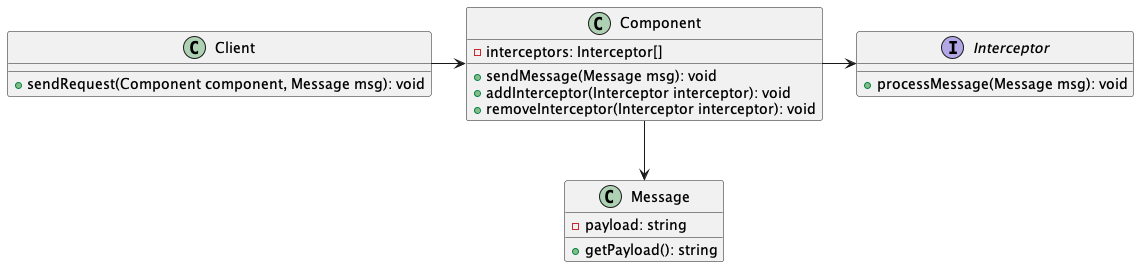
\includegraphics[width=0.99\textwidth]{fig/uml/intercept-class.png}
  \caption{Interceptor Pattern}
  \label{fig:intercept-class}
\end{figure}

Die Verwendung des Interceptor Patterns bietet mehrere Vorteile, wie z.B. die Möglichkeit, die Funktionalität einer Anwendung flexibel zu erweitern, ohne Änderungen am Quellcode der Anwendung selbst vornehmen zu müssen. Es ermöglicht auch eine effektive Steuerung der Kommunikation zwischen Komponenten und kann dazu beitragen, die Sicherheit, Leistung und Zuverlässigkeit der Anwendung zu verbessern.

\begin{figure}[!ht]
  \centering
  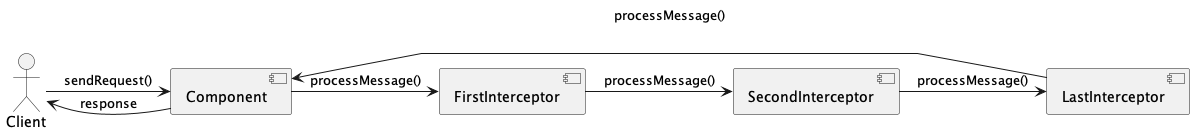
\includegraphics[width=0.99\textwidth]{fig/uml/intercept-seq.png}
  \caption{Interceptor Pattern Sequenz}
  \label{fig:intercept-seq}
\end{figure}

In diesem Beispiel~\ref{fig:intercept-seq} besteht die Component aus einer Kette von Interceptor-Komponenten (FirstInterceptor, SecondInterceptor und LastInterceptor), die die eingehenden Nachrichten abfangen und modifizieren können. Die Client-Komponente sendet eine Nachricht an die Component, die dann durch die Kette von Interceptor-Komponenten läuft, bevor sie an die Client-Komponente zurückgesendet wird.

Das Klassendiagramm~\ref{fig:intercept-class} zeigt die verschiedenen Klassen und deren Beziehungen zueinander, während das Sequenzdiagramm zeigt, wie die verschiedenen Komponenten miteinander interagieren. In beiden Diagrammen ist die Verwendung des Interceptor Patterns deutlich zu erkennen.

Insgesamt ist das Interceptor Pattern ein nützliches Pattern für die Entwicklung von verteilten Systemen, da es eine effektive Möglichkeit bietet, die Kommunikation zwischen Komponenten zu steuern und die Funktionalität der Anwendung zu erweitern.

Ein Beispiel für das Interceptor Pattern in einem verteilten System könnte wie folgt aussehen:
\\\\
Annahmen:\\
\begin{itemize}   
\item Es gibt eine Anwendung, die aus mehreren Komponenten besteht, die über ein Netzwerk miteinander kommunizieren.
\item Eine dieser Komponenten ist für die Ausführung von Finanztransaktionen verantwortlich.
\end{itemize}   
Anforderungen:
\begin{itemize}   
\item Es ist erforderlich, dass alle eingehenden und ausgehenden Finanztransaktionsnachrichten überwacht werden, um die Sicherheit und Integrität der Transaktionen zu gewährleisten.
\item Es ist auch erforderlich, dass die Leistung der Finanztransaktionen überwacht wird, um sicherzustellen, dass die Anwendung reibungslos läuft.
\end{itemize}   
Implementierung:
\begin{itemize}   
\item Das Interceptor Pattern wird eingesetzt, um eine Kette von Interceptor-Komponenten zu erstellen, die die eingehenden und ausgehenden Finanztransaktionsnachrichten abfangen und modifizieren können.
\item Der erste Interceptor in der Kette ist für die Überprüfung der Sicherheit der Finanztransaktionsnachrichten verantwortlich. Wenn die Nachricht sicherheitsrelevant ist, wird sie an den nächsten Interceptor weitergeleitet. Wenn die Nachricht jedoch als unsicher eingestuft wird, wird sie abgelehnt.
\item Der zweite Interceptor in der Kette ist für die Überwachung der Leistung der Finanztransaktionen verantwortlich. Wenn die Nachricht eine Finanztransaktion ist, wird die Leistung der Transaktion gemessen und protokolliert.
\item Der letzte Interceptor in der Kette ist für das Senden der Finanztransaktionsnachricht an die Zielkomponente verantwortlich.
\end{itemize} 
Durch die Verwendung des Interceptor Patterns können die Finanztransaktionen sicher und effektiv überwacht werden, ohne dass Änderungen am Quellcode der Anwendung selbst vorgenommen werden müssen. Die Interceptor-Komponenten können auch problemlos hinzugefügt, entfernt oder geändert werden, um den Anforderungen der Anwendung gerecht zu werden.

\subsubsection{Fassade Pattern}
Das Fassade Pattern ist ein Strukturpattern, das in verteilten Systemen verwendet werden kann, um eine vereinfachte Schnittstelle für den Zugriff auf komplexe Subsysteme bereitzustellen. Es dient als eine Art vereinfachte Schicht, die die Interaktion zwischen Client-Code und einem komplexen Subsystem abstrahiert.

In verteilten Systemen kann das Fassade Pattern genutzt werden, um die Komplexität von Systemen zu reduzieren, indem eine einzige Schnittstelle bereitgestellt wird, die als Einstiegspunkt für den Zugriff auf das System dient. Dies kann dazu beitragen, die Komplexität des Systems für den Benutzer zu reduzieren und die Wartbarkeit des Codes zu verbessern.

Das Fassade Pattern besteht aus einer Fassadenklasse, die eine vereinfachte Schnittstelle für den Zugriff auf ein komplexes Subsystem bereitstellt. Die Fassade delegiert dann die Anfragen des Clients an das Subsystem, um die gewünschten Aktionen auszuführen. Die Fassadeklasse kapselt somit das komplexe Subsystem und stellt dem Client nur eine einfachere Schnittstelle zur Verfügung.

Ein Beispiel für die Verwendung des Fassade Patterns in verteilten Systemen könnte die Verwendung einer zentralen Authentifizierungs- und Autorisierungsschicht sein. Eine Fassadenklasse könnte erstellt werden, die als Schnittstelle für den Zugriff auf diese Schicht fungiert. Die Fassadenklasse könnte dann die Anfragen des Clients an das Authentifizierungs- und Autorisierungssystem weiterleiten, um die gewünschten Aktionen auszuführen.
\\\\
In diesem Beispiel~\ref{lst:fassade} besteht das komplexe Subsystem aus den Klassen SubsystemA und SubsystemB, die jeweils eine komplexe Logik ausführen. Die Facade-Klasse ist die vereinfachte Schnittstelle für den Client und delegiert die Anfragen des Clients an das Subsystem, um die gewünschten Aktionen auszuführen. In diesem Fall führt die performAction()-Methode der Fassade einfach die Operationen von SubsystemA und SubsystemB aus.

Der Client-Code erstellt eine Instanz der Fassade und ruft die performAction()-Methode auf, um auf das komplexe Subsystem zuzugreifen. Die Fassade kapselt somit das komplexe Subsystem und stellt dem Client nur eine einfachere Schnittstelle zur Verfügung.

\noindent\begin{minipage}{\textwidth}
\begin{lstlisting}[caption={Fassade Pattern},captionpos=b,label={lst:fassade}]
// Das komplexe Subsystem
class SubsystemA {
    public void operationA() {
        // komplexe Logik
    }
}

class SubsystemB {
    public void operationB() {
        // komplexe Logik
    }
}

// Die Fassade
class Facade {
    private SubsystemA subsystemA;
    private SubsystemB subsystemB;
    
    public Facade() {
        this.subsystemA = new SubsystemA();
        this.subsystemB = new SubsystemB();
    }
    
    // Einfache Schnittstelle fuer den Client
    public void performAction() {
        subsystemA.operationA();
        subsystemB.operationB();
    }
}

// Client Code
class Client {
    public static void main(String[] args) {
        Facade facade = new Facade();
        facade.performAction();
    }
}
\end{lstlisting}
\end{minipage}


\subsubsection{Pipeline Pattern}
Das Pipeline Pattern ist ein Architekturmuster für verteilte Systeme, das es ermöglicht, komplexe Verarbeitungsprozesse aufzubauen, indem die Verarbeitung in einzelne Schritte aufgeteilt wird, die sequentiell ausgeführt werden. Jeder Schritt wird von einem spezialisierten Modul durchgeführt, das in der Lage ist, einen bestimmten Verarbeitungsschritt auszuführen.

Im Pipeline Pattern gibt es drei grundlegende Komponenten:
\begin{itemize} 
\item Die Pipeline: eine Abfolge von Verarbeitungsschritten, die in einer bestimmten Reihenfolge ausgeführt werden.
\item Die Module: spezialisierte Komponenten, die für die Durchführung jedes Verarbeitungsschritts verantwortlich sind.
\item Die Daten: die Eingabe- oder Ausgabedaten, die durch die Pipeline fließen und von den Modulen verarbeitet werden.
\end{itemize} 
Ein Beispiel für das Pipeline Pattern könnte ein System sein, das große Datenmengen verarbeiten muss. Die Daten könnten in mehrere Schritte unterteilt werden, wie z.B. das Lesen von Daten aus einer Quelle, das Filtern von Daten, das Aggregieren von Daten und das Speichern von Daten in einer Datenbank. Jeder dieser Schritte wird von einem spezialisierten Modul durchgeführt, das in der Lage ist, diesen Verarbeitungsschritt effizient auszuführen.

Das Pipeline Pattern bietet eine Vielzahl von Vorteilen für verteilte Systeme, wie z.B. eine bessere Skalierbarkeit und Flexibilität bei der Entwicklung von komplexen Verarbeitungsprozessen. Es ermöglicht auch eine bessere Wiederverwendbarkeit von Modulen und eine einfachere Wartung und Fehlerbehebung. Allerdings erfordert das Pipeline Pattern auch eine sorgfältige Planung und Gestaltung der einzelnen Verarbeitungsschritte und Module, um eine optimale Leistung und Skalierbarkeit zu gewährleisten.

\subsubsection{Watchdog}
Das Watchdog Pattern ist ein bekanntes Entwurfsmuster in der Softwareentwicklung, das zur Überwachung von Ressourcen oder Prozessen in einem System verwendet wird. Es ist besonders nützlich, um potenzielle Fehler oder Störungen frühzeitig zu erkennen und entsprechende Maßnahmen zu ergreifen, um die Stabilität und Zuverlässigkeit der Anwendung zu gewährleisten.

Im Wesentlichen besteht das Watchdog Pattern aus zwei Hauptkomponenten: dem Watchdog und dem überwachten System oder Prozess. Der Watchdog ist ein unabhängiger Prozess, der den Zustand und das Verhalten des überwachten Systems kontinuierlich überprüft. Dazu verwendet der Watchdog bestimmte Prüfkriterien oder Zeitintervalle, um festzustellen, ob das überwachte System ordnungsgemäß funktioniert oder ob es Anzeichen für Fehlfunktionen gibt.

Sollte der Watchdog feststellen, dass das überwachte System nicht mehr ordnungsgemäß funktioniert, kann er entsprechende Maßnahmen ergreifen, um das Problem zu beheben. Dies kann beispielsweise das Neustarten des fehlerhaften Prozesses, das Senden einer Benachrichtigung an einen Administrator oder das Ausführen von Fallback- oder Wiederherstellungsmechanismen sein.

Das Watchdog Pattern ist in verschiedenen Anwendungsbereichen, wie zum Beispiel eingebetteten Systemen, verteilten Systemen oder auch bei der Überwachung von Softwarekomponenten, sehr nützlich. Es hilft dabei, die Systemverfügbarkeit und -stabilität zu erhöhen und die Auswirkungen von Fehlern oder Störungen zu minimieren.

Ein wichtiger Aspekt bei der Implementierung des Watchdog Patterns ist die Trennung der Verantwortlichkeiten zwischen dem Watchdog und dem überwachten System. Der Watchdog sollte so unabhängig wie möglich vom überwachten System agieren, um sicherzustellen, dass er selbst nicht von den Problemen betroffen ist, die er überwachen soll. Dies kann beispielsweise durch die Verwendung von separaten Prozessen oder Threads erreicht werden.

Insgesamt ist das Watchdog Pattern ein leistungsfähiges Entwurfsmuster, das dazu beiträgt, die Robustheit und Zuverlässigkeit von Softwaresystemen zu erhöhen. Durch die frühzeitige Erkennung und Behebung von Problemen kann es dazu beitragen, die Ausfallzeiten und die potenziellen Auswirkungen auf Benutzer und Kunden zu reduzieren.

\subsubsection{Master-Worker Pattern}
Das Master-Worker Pattern, auch bekannt als Master-Slave Pattern, ist ein grundlegendes Entwurfsmuster in der Informatik, das speziell für verteilte Systeme entwickelt wurde. Es ist eine Methode zur Organisation von Systemen, bei der eine zentrale Einheit (Master) die Kontrolle über mehrere untergeordnete Einheiten (Worker) hat. Das Hauptziel dieses Musters ist es, die Arbeitslast effizient auf mehrere Prozessoren oder Knoten zu verteilen und die Skalierbarkeit und Zuverlässigkeit des Gesamtsystems zu verbessern.

In verteilten Systemen der Informatik ist das Master-Worker Pattern von großer Bedeutung, da es die folgenden Vorteile bietet:
\begin{itemize} 
\item Parallelisierung: Das Muster erlaubt die Aufteilung von Arbeitslasten auf mehrere Worker, wodurch Aufgaben parallel und somit schneller ausgeführt werden können. Dies ist besonders nützlich bei rechenintensiven Aufgaben und bei Systemen, bei denen Ressourcen effizient genutzt werden müssen.
\item Skalierbarkeit: Das Master-Worker Pattern ermöglicht es, einem System einfach neue Worker hinzuzufügen oder bestehende Worker zu entfernen, um die Systemleistung je nach Bedarf anzupassen. Dadurch kann das System auch bei wachsenden Anforderungen weiterhin effizient arbeiten.
\item Fehlertoleranz: Da das System aus mehreren unabhängigen Workern besteht, kann es bei einem Ausfall eines Workers immer noch weiterarbeiten. Der Master kann den ausgefallenen Worker ersetzen oder dessen Aufgaben auf andere Worker verteilen, um sicherzustellen, dass das System trotz des Ausfalls weiterhin funktioniert.
\item Vereinfachung der Anwendungsentwicklung: Das Master-Worker Pattern ermöglicht es den Entwicklern, ihre Anwendungen zu modularisieren, indem sie die Funktionalität auf verschiedene Worker aufteilen. Dadurch können Entwickler sich auf einzelne Teilaufgaben konzentrieren, was die Anwendungsentwicklung und -wartung vereinfacht.
\end{itemize}    

Ein Beispiel für die Verwendung des Master-Worker Patterns ist das MapReduce-Paradigma, das in verteilten Datenverarbeitungssystemen wie Hadoop verwendet wird. Der Master, auch als \enquote{Jobtracker} bezeichnet, teilt die Eingabedaten in kleinere Teile auf und weist diese den Workern, auch als \enquote{Tasktracker} bezeichnet, zur Verarbeitung zu. Die Worker führen ihre zugewiesenen Aufgaben aus und melden ihre Ergebnisse zurück an den Master, der diese dann zu einem einzigen Ergebnis zusammenführt.

Es wurde erstmals von Google im Jahr 2004 eingeführt und ist seitdem zu einem grundlegenden Baustein in der Verarbeitung großer Datenmengen geworden, insbesondere im Bereich des Big Data und der Datenanalyse.

MapReduce besteht aus zwei Hauptphasen: Map und Reduce.
\begin{itemize}  
\item Map-Phase: In dieser Phase werden die Eingabedaten in Key-Value-Paare aufgeteilt und anschließend parallel über die verfügbaren Knoten im Cluster verteilt. Die Map-Funktion wird auf jedem dieser Knoten ausgeführt und verarbeitet die zugeordneten Key-Value-Paare. Die Ausgabe der Map-Funktion ist eine Liste von Zwischen-Key-Value-Paaren.
\item Reduce-Phase: Die Zwischen-Key-Value-Paare aus der Map-Phase werden nach dem Schlüssel gruppiert und an die Reduce-Funktion weitergeleitet. Die Reduce-Funktion wird auf jedem Gruppenschlüssel ausgeführt und fasst die zugehörigen Werte zusammen, um die endgültigen Ergebnisse zu erzeugen.
\end{itemize}  

Ein einfaches Beispiel für das MapReduce-Paradigma ist die Wortzählung in einem Text. Angenommen, wir haben einen großen Text und möchten die Häufigkeit jedes Wortes zählen. Hier ist, wie wir dies mit MapReduce erreichen können:
\begin{itemize} 
\item Map-Phase: Zuerst wird der Text in kleinere Abschnitte aufgeteilt und auf verschiedene Knoten im Cluster verteilt. Die Map-Funktion wird auf jedem Knoten ausgeführt, um jedes Wort in den Abschnitten zu verarbeiten.

Die Map-Funktion liest die Wörter in ihrem zugewiesenen Abschnitt und erstellt ein Key-Value-Paar für jedes Wort, wobei der Schlüssel das Wort selbst ist und der Wert 1. Wenn das Wort "Hallo" beispielsweise dreimal im Abschnitt erscheint, gibt die Map-Funktion folgende Key-Value-Paare aus:

\noindent\begin{minipage}{\textwidth}
\begin{lstlisting}[caption={Ausgabe},captionpos=b,label={lst:map}]
("Hallo", 1)
("Hallo", 1)
("Hallo", 1)
\end{lstlisting}
\end{minipage}

\item Reduce-Phase: Nachdem die Map-Phase abgeschlossen ist, werden die Key-Value-Paare nach dem Schlüssel (Wort) gruppiert und an die Reduce-Funktion gesendet. In diesem Fall hätten wir eine Gruppe für das Wort \enquote{Hallo} mit den Werten [1, 1, 1].

Die Reduce-Funktion summiert die Werte für jedes Wort, um die endgültige Häufigkeit zu erhalten. Für das Wort \enquote{Hallo} würde die Reduce-Funktion die Werte addieren (1 + 1 + 1) und das endgültige Key-Value-Paar ausgeben:
\noindent\begin{minipage}{\textwidth}
\begin{lstlisting}[caption={Ausgabe},captionpos=b,label={lst:map}]
("Hallo", 3)
\end{lstlisting}
\end{minipage}
\end{itemize}  

Nachdem alle Reduce-Funktionen ausgeführt wurden, haben wir eine Liste von Key-Value-Paaren, die die Häufigkeit jedes Wortes im gesamten Text angeben.

Dieses Beispiel veranschaulicht die grundlegenden Schritte des MapReduce-Paradigmas. In der Praxis würde ein MapReduce-Framework wie Apache Hadoop diese Phasen automatisch auf einem Cluster von Computern ausführen und die Verarbeitung von großen Datenmengen ermöglichen.

%Termin-5 - vs-slides-chapter02-3
%Termin-5 - vs-slides-chapter02-4

\subsection{Beispielarchitekturen}
Die Remote Procedure Call (RPC) Architektur und die Peer-to-Peer (P2P) Architektur sind zwei grundlegend unterschiedliche Ansätze zur Entwicklung verteilter Systeme, die jeweils ihre eigenen Stärken und Schwächen aufweisen. Beide Architekturen bieten Lösungen für verschiedene Anwendungsfälle und Probleme, die in verteilter Systementwicklung auftreten. Durch das Vergleichen dieser beiden Beispielarchitekturen können wir ein besseres Verständnis der verschiedenen Aspekte und Herausforderungen bei der Entwicklung verteilter Systeme gewinnen.
\subsubsection{Remote Procedure Call}

Die Remote Procedure Call (RPC) Architektur ist ein Kommunikationsmodell, das es ermöglicht, Prozeduraufrufe zwischen Prozessen auf unterschiedlichen Systemen oder Maschinen durchzuführen. Die Idee hinter RPC besteht darin, entfernte Funktionen oder Methoden so einfach aufrufen zu können, als wären sie lokale Funktionen innerhalb des aufrufenden Programms.
\\\\
Aufbau einer RPC-Architektur:
\begin{itemize} 
\item Client: Der Client ist der Prozess oder die Anwendung, die den entfernten Prozeduraufruf initiiert. Der Client stellt eine Anfrage an den Server, um eine bestimmte Funktion auszuführen, und wartet auf die Antwort.
\item Client Stub: Der Client Stub ist eine lokale Repräsentation der entfernten Prozedur auf der Clientseite. Er ist dafür verantwortlich, die Anfrage des Clients in ein geeignetes Format umzuwandeln, das vom Server verstanden werden kann. Dieser Vorgang wird als \enquote{Marshalling} bezeichnet.
\item Kommunikationsprotokoll: Ein Kommunikationsprotokoll wird verwendet, um die Anfrage und die Antwort zwischen Client und Server zu übertragen. Dies kann beispielsweise ein TCP/IP- oder UDP-Protokoll sein, je nach den Anforderungen an Zuverlässigkeit, Geschwindigkeit und Latenz.
\item Server: Der Server ist der Prozess oder die Anwendung, die die angeforderte Funktion oder Methode bereitstellt. Der Server empfängt die Anfrage vom Client, führt die entsprechende Prozedur aus und sendet die Antwort zurück.
\item Server Stub: Der Server Stub empfängt die Anfrage vom Client, wandelt sie in ein für die Serverumgebung geeignetes Format um (\enquote{Unmarshalling}) und ruft die gewünschte Funktion auf. Anschließend werden die Ergebnisse wieder \enquote{gemarshalled} und an den Client gesendet.
\end{itemize}     

Im Folgenden wird der grundsätzliche Ablauf in einer RPC Architektur beschrieben, welcher noch verfeinert werden sollte, aber bereits die grundlegende Idee transportiert. 

\begin{enumerate} 
\item Der Client ruft die entfernte Prozedur über den Client Stub auf, als wäre es eine lokale Funktion.
\item Der Client Stub wandelt die Parameter der Anfrage in ein standardisiertes Format um (Marshalling) und sendet die Anfrage über das Kommunikationsprotokoll an den Server.
\item Der Server Stub empfängt die Anfrage, demarshalled die Parameter und ruft die entsprechende Funktion auf dem Server auf.
\item Die Funktion wird auf dem Server ausgeführt, und das Ergebnis wird an den Server Stub zurückgegeben.
\item Der Server Stub marshallt das Ergebnis und sendet es über das Kommunikationsprotokoll an den Client Stub zurück.
\item Der Client Stub empfängt die Antwort, demarshalled das Ergebnis und gibt es an den Client zurück.
\end{enumerate}

In einer RPC-Architektur kann die Kommunikation sowohl synchron als auch asynchron erfolgen. Bei synchroner Kommunikation wartet der Client auf die Antwort vom Server, bevor er weitere Aktionen ausführt. Dies kann zu Wartezeiten führen, insbesondere bei langsamen Netzwerkverbindungen oder komplexen Anfragen. Bei asynchroner Kommunikation sendet der Client die Anfrage und führt sofort weitere Aufgaben aus, ohne auf die Antwort zu warten. Die Antwort wird in der Regel über einen Callback-Mechanismus oder ein Event-System verarbeitet, sobald sie verfügbar ist.

Die RPC-Architektur ist in verschiedenen Anwendungen und Umgebungen weit verbreitet, wie z.B. bei verteilten Systemen, Client-Server-Anwendungen und Microservices. Sie bietet eine abstrakte und einfach zu verwendende Schnittstelle für die Kommunikation zwischen Prozessen auf verschiedenen Systemen, ohne dass sich der Entwickler um die Details der Netzwerkkommunikation kümmern muss.

Das Diagramm~\ref{fig:simple-rpc} zeigt einen ersten naiven Entwurf einer RPC Schichtenarchitektur. In diesem Ansatz existiert eine Schicht \enquote{Application}, welche die Schicht der Middleware nutzt, welche wiederum die Ressourcen - beispielhaft des Betriebssystems - nutzt, um die Kommunikation mittels Netzwerkprotokolle zu realisieren. 

\begin{figure}[!ht]
  \centering
  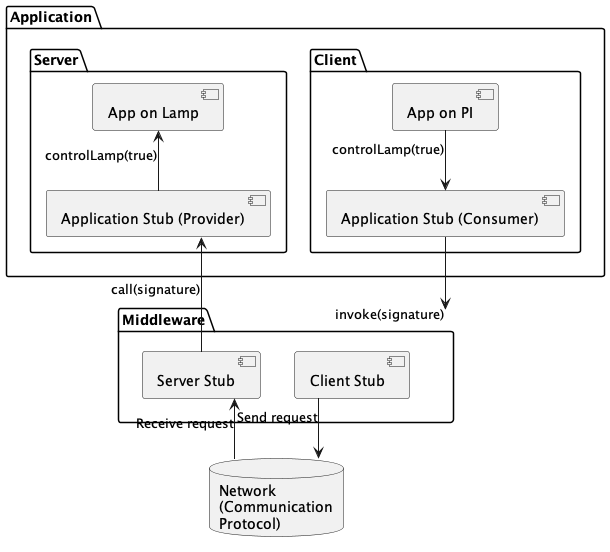
\includegraphics[width=0.95\textwidth]{fig/uml/rpc-simple.png}
  \caption{Erster Ansatz einer RPC Architektur}
  \label{fig:simple-rpc}
\end{figure}

Interessant ist die Einbringung einer zusätzlichen Schicht in der Applikation, die als Application Stub bezeichnet ist. Die Idee des Application-Stubs (auch als \enquote{Applikations-Stub} oder \enquote{App-Stub} bezeichnet) wurde von Andrew S. Tanenbaum entwickelt, um die Kommunikation und Interaktion zwischen Anwendungen und Middleware in verteilten Systemen zu erleichtern. Der Application-Stub ist eine Schnittstelle, die als Vermittler zwischen der Anwendung und der Middleware fungiert, um die Kommunikation und Zusammenarbeit zwischen diesen beiden Ebenen zu ermöglichen.

Die Umsetzung des Application-Stubs basiert auf der Trennung der Anwendungslogik von der Middleware-Kommunikationslogik. Dies wird erreicht, indem der Stub die Anwendungslogik von den Netzwerkdetails, wie z.B. den Marshalling/Unmarshalling von Daten, dem Verbindungsaufbau und dem Senden/Empfangen von Nachrichten, entkoppelt.

Um den Application-Stub in einer verteilten Umgebung zu nutzen, sind folgende Schritte erforderlich:
\begin{itemize} 
\item Entwurf einer Schnittstellenbeschreibung: Zunächst wird eine Schnittstellenbeschreibung erstellt, die die Funktionen und Methoden definiert, die von der Anwendung und der Middleware bereitgestellt werden sollen. Diese Schnittstellenbeschreibung kann in einer Interface Definition Language (IDL) oder einer ähnlichen Sprache definiert werden.
\item Erstellung des Application-Stubs: Basierend auf der Schnittstellenbeschreibung wird ein Application-Stub generiert oder manuell erstellt. Dieser Stub enthält Code, der die Kommunikation zwischen der Anwendung und der Middleware verwaltet. Es kann für verschiedene Programmiersprachen und Plattformen erstellt werden, um die Interoperabilität zu gewährleisten.
\item Integration des Application-Stubs in die Anwendung: Der generierte oder erstellte Application-Stub wird in die Anwendung integriert, indem er die definierten Funktionen und Methoden für die Kommunikation mit der Middleware implementiert. Die Anwendung ruft die Funktionen und Methoden des Stubs auf, als wären sie lokale Funktionen oder Methoden, ohne sich um die zugrunde liegenden Netzwerkdetails kümmern zu müssen. Das Factory Pattern kann hier eine Lösung sein, die Wahl zu implementieren.
\item Anpassung der Middleware: Die Middleware muss in der Lage sein, die Anfragen des Application-Stubs zu verarbeiten und entsprechend zu reagieren. Dies kann durch die Implementierung von Server-Stubs und der entsprechenden Kommunikationslogik erreicht werden.
\item Kommunikation zwischen Anwendung und Middleware: Durch die Verwendung des Application-Stubs kann die Anwendung nun nahtlos mit der Middleware kommunizieren, ohne sich um die Details der Netzwerkkommunikation kümmern zu müssen. Die Middleware empfängt die Anfragen, verarbeitet sie und sendet die Ergebnisse zurück an die Anwendung über den Application-Stub.
\end{itemize} 
Die Verwendung eines Application-Stubs bietet mehrere Vorteile, wie z.B.:
\begin{itemize} 
\item Entkopplung der Anwendungslogik von der Middleware-Kommunikationslogik, was zu einer besseren Trennung von Verantwortlichkeiten und einfacherer Wartung führt.
\item Vereinfachung der Kommunikation zwischen Anwendung und Middleware durch Abstraktion der Netzwerkdetails, sodass sich Entwickler auf die Anwendungslogik konzentrieren können.
\item Erhöhung der Interoperabilität zwischen Anwendungen und Middleware, da der Application-Stub in verschiedenen Programmiersprachen und Plattformen implementiert werden kann.
\item Verbesserung der Modularität und Skalierbarkeit von verteilten Systemen, da Anwendungen und Middleware unabhängig voneinander entwickelt, aktualisiert und erweitert werden können.
\end{itemize} 

Der Application-Stub ermöglicht nach Tanenbaum eine effiziente Kommunikation und Zusammenarbeit zwischen Anwendungen und Middleware in verteilten Systemen. Durch die Entkopplung der Anwendungslogik von der Kommunikationslogik können Entwickler sich auf die wesentlichen Aspekte der Anwendung konzentrieren, während die Middleware die Netzwerkkommunikation und andere Details verwaltet.
\\\\
Hier ist ein einfaches Beispiel in Java, das die Idee des Application-Stubs und das Factory-Pattern verwendet, um eine Anwendung mit Middleware zu verbinden. In diesem Beispiel simulieren wir eine einfache Lampe und ihre Steuerung.
Zuerst erstellen wir eine Lamp-Schnittstelle, die als Middleware fungiert:\\
\noindent\begin{minipage}{\textwidth}
\begin{lstlisting}[caption={RPC Interface},captionpos=b,label={lst:rpc-interface}]
public interface Lamp {
    void controlLamp(Boolean b);
}
\end{lstlisting}
\end{minipage}
Als nächstes erstellen wir eine Implementierung der Lamp-Schnittstelle auf dem Server-Anteil des Applikationscodes:\\

\noindent\begin{minipage}{\textwidth}
\begin{lstlisting}[caption={RPC Remote Implementation},captionpos=b,label={lst:rpc-remote}]
public class LampRemote implements Lamp {
    @Override
    public void controlLamp(boolean b){
    	List<Boolean> list = new ArrayList<Boolean>(); 
        Collections.addAll(list, b);
        Middleware.invoke("controlLamp", list);
    }
}
\end{lstlisting}
\end{minipage}
Nun erstellen wir eine Factory-Klasse, die als Application-Stub fungiert:\\
\noindent\begin{minipage}{\textwidth}
\begin{lstlisting}[caption={Application Stub mit Factory Pattern},captionpos=b,label={lst:rpc-factory}]
public class LampFactory {
    public static Lamp createLamp() {
        // Hier koennte die Middleware-Verbindung hergestellt werden.
        // In diesem Beispiel verwenden wir eine einfache lokale Implementierung.
        return new LampRemote();
    }
}
\end{lstlisting}
\end{minipage}
Schließlich erstellen wir eine Anwendungsklasse, die die Lamp-Schnittstelle verwendet:\\
\noindent\begin{minipage}{\textwidth}
\begin{lstlisting}[caption={Controller ruft Middleware},captionpos=b,label={lst:rpc-controller}]
public class LampController {
	public static void main(String[] args) {
        // Erstelle eine Lampe ueber die Factory-Methode (Application-Stub)
        Lamp lamp = LampFactory.createLamp();

        // Verwende die Lampe in der Anwendung
        lamp.controlLamp(true);
    }
}
\end{lstlisting}
\end{minipage}
In diesem Beispiel wurde eine Lamp-Schnittstelle erstellt, die als Middleware fungiert, um eine Lampe zu steuern. Die LampFactory-Klasse dient als Application-Stub, der die Erstellung und Verbindung zur Middleware verwaltet. Die Lamp Controller-Anwendung verwendet die Lamp-Schnittstelle über die Factory-Methode, um die Lampe ein- und auszuschalten.

In einer realen Anwendung könnte die LampFactory-Klasse die Verbindung zu einer tatsächlichen Middleware herstellen, anstatt einfach eine lokale Implementierung zu erstellen. Natürlich ist die Annahme einer Objektmenge nur aus dem Datentyp Boolean naiv, zeigt aber die Funktionsweise ausreichend auf. Die Anwendung selbst muss sich jedoch nicht um diese Details kümmern, da der Application-Stub diese Verantwortung übernimmt.

Diese zunächst einfache und naive Darstellung ist als Möglichkeit gedacht, um zunächst einen Überblick zu schaffen. Natürlich müssen hier verschiedene Aspekte verfeinert und für das bessere Verständnis nochmal diskutiert werden. 

Als erstes muss man festhalten, dass aus der naiven Ansicht häufig ein Verhalten abgeleitet wird, welches aber auf einer missverstandenen Interpretation der Architektur zurückzuführen ist, weniger auf ein noch nicht eingeführtes Verhaltensdiagramm. 
\\\\
Ist die Beschreibung des Verhaltens in der Architektur das Ziel, muss nochmals auf die Nutzung des Schichtenmodells hingewiesen werden. Jede Schicht kapselt die Sequenzen nach der zugeordneten Verantwortlichkeit.
Somit beschreiben die Sequenzen in der Applikationsschicht die der Applikation und die Sequenzen der Middleware die der Middleware. Was nicht geschehen sollte, ist eine Vermischung beider Schichten. So wäre eine gültige Sequenz der Applikation beschrieben in Diagramm~\ref{fig:rpc-app-seq-rpc} und eine der Middleware im Diagramm~\ref{fig:rpc-middleware-seq-rpc}. An der Sequenz in der Applikation selbst sollte man nicht ohne weiteres erkennen, dass es sich um einen entfernen Funktionsaufruf handelt. Diese Aufgabe wird von der Middleware übernommen.
\\\\
Es ist wichtig zu verstehen, dass die Sequenz der Applikation aus einer spezifischen Verarbeitung des Anwendungsfalls getrieben ist, wohingegen die Sequenz der Middleware eine generische Umsetzung repräsentiert, die von jeglichem Aufruf aus der Applikation heraus genutzt werden kann. So kann man naiv die Beziehung zwischen einem entfernten Funktionsaufruf und der Middleware auch als eine 0:n- Beziehung beschreiben, wobei die Middleware  in diesem Fall eine generische Funktion für einen synchronen Funktionsaufruf repräsentiert. 


 \begin{figure}[!ht]
  \centering
  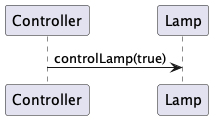
\includegraphics[width=0.30\textwidth]{fig/uml/rpc-app-seq.png}
  \caption{Beispielsequenz der App in der RPC Architektur}
  \label{fig:rpc-app-seq-rpc}
\end{figure}


 \begin{figure}[!ht]
  \centering
  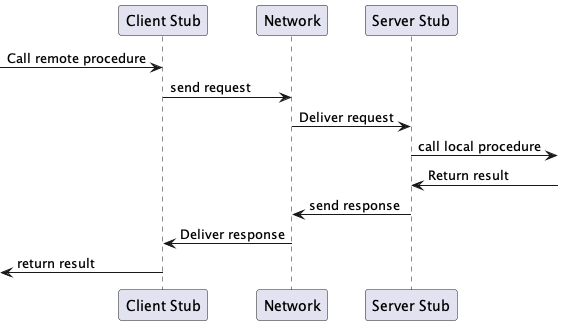
\includegraphics[width=0.65\textwidth]{fig/uml/rpc-middleware-seq.png}
  \caption{Beispielsequenz der Middleware in der RPC Architektur}
  \label{fig:rpc-middleware-seq-rpc}
\end{figure}

Um die Middleware möglichst transparent und wiederverwendbar zu gestalten, soll der Marshalling-Prozess genauer betrachtet werden, der im Client-Stub und Server-Stub eine besondere Rolle spielt, bevor die Nachrichten für den entfernten Funktionsaufruf versendet werden. 

Der Marshalling-Prozess und die Serialisierung sind Begriffe, die oft im Zusammenhang mit der Remote Procedure Call (RPC) Architektur verwendet werden. Beide Prozesse sind zwar miteinander verknüpft, es gibt jedoch grundlegende Unterschiede zwischen ihnen.
\\\\
Der Marshalling-Prozess ist ein Verfahren, bei dem Daten und Parameter in einer Form gewandelt werden, die über das Netzwerk gesendet und auf der anderen Seite wieder zusammengesetzt werden kann. Kurz: aus einem Funktionsaufruf wird eine Nachricht generiert. Dieser Prozess ist in der RPC-Architektur besonders wichtig, da hierdurch entfernte Prozeduraufrufe zwischen verschiedenen Systemen mit unterschiedlichen Datenformaten, Speicherlayouts oder sogar Programmiersprachen umgesetzt werden können.
\\\\
Der Marshalling-Prozess besteht aus mehreren Schritten:
\begin{itemize} 
\item Umwandlung der Daten und Parameter in ein plattformunabhängiges Format, oft in Form von Byte-Arrays.
\item Anfügen von Metadaten, wie zum Beispiel Typinformationen, um den Empfänger darüber zu informieren, wie die Daten wiederhergestellt werden können.
\item Zusammenpacken (Packing) der Daten und Metadaten in einer Nachricht, die über das Netzwerk gesendet werden kann.
\end{itemize} 

Die Serialisierung ist der Prozess der Umwandlung eines Objekts oder einer Datenstruktur in eine lineare, sequenzielle Darstellung, die zum Speichern oder Übertragen über ein Netzwerk verwendet werden kann. Serialisierung ist ein wichtiger Teil des Marshalling-Prozesses, da sie die Daten in eine übertragbare Form konvertiert. Sie ermöglicht es, den Zustand eines Objekts oder einer Datenstruktur zu erhalten, sodass es auf der Empfängerseite wiederhergestellt und verwendet werden kann. Unterschiede zwischen Marshalling und Serialisierung:
\begin{itemize} 
\item Anwendungsbereich: Serialisierung ist ein generischer Prozess, der nicht nur in der RPC-Architektur, sondern auch in anderen Anwendungen wie der persistenten Speicherung von Objekten und der Interprozesskommunikation verwendet wird. Marshalling ist spezifisch für die RPC-Architektur und bezieht sich auf das Vorbereiten von Daten und Parametern für entfernte Prozeduraufrufe.
\item Metadaten: Marshalling beinhaltet das Hinzufügen von Metadaten, die zur Interpretation und Rekonstruktion der übertragenen Daten auf der Empfängerseite erforderlich sind. Bei der Serialisierung werden hauptsächlich die Daten selbst in eine sequenzielle Darstellung umgewandelt, ohne notwendigerweise zusätzliche Metadaten hinzuzufügen.
\end{itemize} 
Im Weiteren soll ein Beispiel für einen Marshalling-Prozess ausgearbeitet werden. Angenommen, es gibt zwei Systeme A und B, die unterschiedliche Programmiersprachen und Datenformate verwenden. System A möchte eine Funktion auf System B aufrufen, die zwei Parameter akzeptiert: einen String und einen Integer. Der Marshalling-Prozess auf System A würde wie folgt aussehen:
\begin{itemize} 
\item Konvertierung der Parameter (z.B. String und Integer) in ein plattformunabhängiges Format, z. B. Byte-Arrays.
\item Hinzufügen von Metadaten, wie Typinformationen, zur Identifizierung der Parameter auf der Empfängerseite.
\item Zusammenpacken der Byte-Arrays und Metadaten in einer Nachricht, die über das Netzwerk gesendet werden kann
\end{itemize} 

Das Ziel, den Marshalling Process möglich generisch zu gestallten, ist in dem Prinzip \enquote{Copy in, Copy out} zusammengefasst. Der Begriff \enquote{Copy in, Copy out} (auch als \enquote{Call by Value-Result} bezeichnet) ist eine Semantik zur Übergabe von Parametern bei entfernten Prozeduraufrufen (RPCs) oder in Programmiersprachen. Es beschreibt die Art und Weise, wie Daten und Parameter zwischen dem aufrufenden und dem aufgerufenen System übertragen werden. Hier ist das grundlegende Prinzip von \enquote{Copy in, Copy out}:
\begin{itemize} 
\item Copy in: Beim Aufruf einer entfernten Funktion kopiert das aufrufende System die Werte der Parameter in eine Nachricht, die an das aufgerufene System gesendet wird. Dieser Schritt beinhaltet den Marshalling-Prozess, bei dem die Parameter in ein plattformunabhängiges Format konvertiert und Metadaten hinzugefügt werden.
\item Copy out: Nachdem die entfernte Funktion auf dem aufgerufenen System ausgeführt wurde, werden die Ergebnisse (Rückgabewerte oder geänderte Parameter) zurück zum aufrufenden System gesendet. Der Rückgabewert und die geänderten Parameter durchlaufen den Marshalling-Prozess erneut, um sie in eine übertragbare Form zu bringen. Anschließend kopiert das aufrufende System die empfangenen Daten in die ursprünglichen Variablen oder Speicherbereiche.
\end{itemize} 
\enquote{Copy in, Copy out} bietet einige Vorteile: Es vermeidet die direkte Manipulation von Speicheradressen zwischen unterschiedlichen Systemen, was bei verteilten Systemen mit unterschiedlichen Speicherlayouts und Adressräumen problematisch sein kann. Weiterhin stellt es sicher, dass das aufgerufene System nur auf Kopien der übergebenen Daten arbeitet, wodurch Seiteneffekte und unerwartete Änderungen der Daten auf dem aufrufenden System vermieden werden. Zuletzt erlaubt es die Verwendung verschiedener Programmiersprachen und Datenformate auf dem aufrufenden und aufgerufenen System, da die Daten beim Marshalling in ein plattformunabhängiges Format konvertiert werden.

Ein Nachteil von \enquote{Copy in, Copy out} ist jedoch der zusätzliche Overhead, der durch das Kopieren und Marshalling/Unmarshalling der Daten entsteht. Dies kann die Leistung und Effizienz des entfernten Prozeduraufrufs beeinträchtigen, insbesondere bei großen Datenmengen oder komplexen Datenstrukturen. In solchen Fällen können andere Parameterübergabemechanismen, wie beispielsweise \enquote{Call by Reference}, in Betracht gezogen werden, bei denen nur die Speicheradressen der Daten übertragen werden und somit der Overhead reduziert wird. 

Allerdings bringt dies auch zusätzliche Herausforderungen und Risiken mit sich, wie zum Beispiel die Notwendigkeit, die unterschiedlichen Adressräume der beteiligten Systeme zu verwalten, und das Risiko unerwarteter Seiteneffekte, wenn das aufgerufene System direkt auf den Speicher des aufrufenden Systems zugreift.

Um den Overhead bei der Verwendung von \enquote{Copy in, Copy out} zu minimieren, können verschiedene Optimierungen angewendet werden, wie zum Beispiel:

\begin{itemize} 
\item Datenkompression: Durch die Komprimierung der Daten während des Mar-shalling-Prozesses kann die Menge der übertragenen Daten reduziert werden, was zu einer schnelleren Übertragung und geringeren Netzwerkbelastung führt.
\item Verwendung effizienter Serialisierungsformate: Einige Serialisierungsformate, wie beispielsweise Protocol Buffers oder MessagePack, sind darauf ausgelegt, Daten effizienter und kompakter zu übertragen als textbasierte Formate wie JSON oder XML.
\item Selektive Übertragung: In einigen Fällen ist es möglich, nur die notwendigen Teile einer Datenstruktur oder eines Objekts zu übertragen, anstatt das gesamte Objekt zu kopieren und zu übertragen. Dies kann den Overhead der Parameterübergabe reduzieren.
\end{itemize} 

Bei der Verwendung von \enquote{Copy in, Copy out} in der RPC-Architektur ist es wichtig, die Datentypen der Parameter und Rückgabewerte korrekt zu bestimmen, um eine erfolgreiche Kommunikation zwischen dem aufrufenden und dem aufgerufenen System zu gewährleisten. 

Mit der \enquote{Copy in, Copy out} Semantik können Prozesse automatisiert werden, um die Codeanteile in einer RPC-Middleware zu bestimmen. Diese automatisierte Code-Generierung kann in folgende Schritte durchgeführt werden:
\begin{itemize} 
\item Definieren der Schnittstellen und Datenstrukturen, die in den entfernten Prozeduraufrufen verwendet werden. Dies geschieht mittels einer Interface Definition Language (IDL). Die IDL beschreibt die Signatur der entfernten Funktionen, einschließlich der Datentypen der Parameter und Rückgabewerte
\item Generieren des Stub- und Skeleton-Codes aus der IDL-Definition. Die meisten RPC-Middleware-Tools bieten Code-Generatoren an, die aus der IDL-Definition automatisch Stub- und Skeleton-Code für verschiedene Programmiersprachen erstellen. Der Stub-Code dient als Proxy für den Aufrufer, während der Skeleton-Code die Implementierung der entfernten Funktion auf dem aufgerufenen System kapselt. Beide Teile des Codes enthalten die notwendigen Informationen über die Datentypen für das Marshalling und Unmarshalling der Daten.
\item Implementierung der entfernten Funktionen auf dem aufgerufenen System unter Verwendung des generierten Skeleton-Codes. Dies stellt sicher, dass die Implementierung der Funktionen mit den in der IDL-Definition angegebenen Datentypen übereinstimmt.
\item  Verwendung des generierten Stub-Codes auf dem aufrufenden System, um entfernte Prozeduraufrufe durchzuführen. Der Stub-Code stellt sicher, dass die Parameter und Rückgabewerte korrekt gemarshalled und unmarshalled werden, basierend auf den in der IDL-Definition festgelegten Datentypen.
\end{itemize} 
Zentrale Komponente ist die  Interface Definition Language (IDL). Eine Interface Definition Language ist eine formale Beschreibungssprache, die verwendet wird, um Schnittstellen zwischen Softwarekomponenten und Diensten in einer standardisierten und plattformunabhängigen Weise zu definieren. Die Verwendung einer IDL in Verbindung mit einem Code-Generator bietet mehrere Vorteile für die automatische Erstellung von Remote Procedure Call Lösungen.

Ein Code-Generator für Interface Definition Language ist ein Software-Tool, das automatisch Code in einer oder mehreren Programmiersprachen auf der Grundlage einer IDL-Definition erstellt. Der Prozess der Codegenerierung aus einer IDL umfasst mehrere Schritte:
\begin{itemize} 
\item Analyse der IDL-Datei: Der Code-Generator liest und analysiert die IDL-Datei, die die Schnittstellendefinitionen, Funktionen, Datenstrukturen und Datentypen enthält, die für die Kommunikation zwischen den verschiedenen Komponenten eines verteilten Systems benötigt werden.
\item Parsen der IDL-Datei: Der Code-Generator verwendet einen Parser, um die IDL-Datei in einen abstrakten Syntaxbaum (AST) oder ein ähnliches internes Format zu zerlegen, dass leichter für die Codegenerierung verwendet werden kann.
\item Code-Generierung: Basierend auf dem internen Format erstellt der Code-Generator automatisch den notwendigen Client- und Server-Code für die Kommunikation über das verteilte System. Dies kann Stub- und Skeleton-Code für verschiedene Programmiersprachen umfassen, die für den Remote Procedure Call verwendet werden.
\item Sprachspezifische Anpassungen: Der Code-Generator berücksichtigt die Besonderheiten der jeweiligen Zielsprache, um sicherzustellen, dass der generierte Code den Konventionen und Syntaxanforderungen dieser Sprache entspricht. Dies umfasst die Anpassung von Datentypen, Namenskonventionen und anderen sprachspezifischen Details.
\item Code-Ausgabe: Schließlich gibt der Code-Generator den erstellten Code als Dateien aus, die in das Zielsystem integriert werden können. Dies ermöglicht Entwicklern, die generierten Stubs und Skeletons in ihrem Projekt zu verwenden, um die definierten Schnittstellen über RPC aufzurufen oder bereitzustellen.
\end{itemize} 

Aus diesen Schritten soll nun ein Beispiel abgeleitet werden, welches auch den manuellen Aufbau einer Lösung beschreibt. Angenommen, es gibt ein verteiltes System, in dem ein Client eine entfernte Funktion \enquote{add} aufrufen möchte, die zwei Integer-Parameter akzeptiert und einen Integer-Wert zurückgibt.

Zunächst wird eine Schnittstelle der entfernten Funktion in einer IDL definiert. \\
\noindent\begin{minipage}{\textwidth}
\begin{lstlisting}[caption={IDL Example},captionpos=b,label={lst:idl-example}]
interface MathService {
  int add(in int a, in int b);
}
\end{lstlisting}
\end{minipage}
Diese IDL-Definition beschreibt eine Schnittstelle namens \enquote{MathService} mit einer Funktion \enquote{add}, die zwei Integer-Parameter (\enquote{a} und \enquote{b}) akzeptiert und einen Integer-Wert zurückgibt.

Aus diesen Informationen kann ein  Stub- und Skeleton-Code generiert werden. Abhängig von der verwendeten RPC-Middleware und Programmiersprache erhalten Sie möglicherweise Klassen oder Module, die die \enquote{MathService}-Schnittstelle implementieren und die notwendigen Informationen über die Datentypen enthalten.

Danach ist die \enquote{add}-Funktion auf dem aufgerufenen System unter Verwendung des generierten Skeleton-Codes zu implementieren. So könnte eine Implementierung aussehen:\\
\noindent\begin{minipage}{\textwidth}
\begin{lstlisting}[caption={RPC IDL Service Impl},captionpos=b,label={lst:idl-impl}]
class MathServiceImpl(MathService):
    def add(self, a, b):
        return a + b
\end{lstlisting}
\end{minipage}
Nun kann der generierte Stub-Code auf dem aufrufenden System genutzt werden, um die \enquote{add}-Funktion über einen RPC-Aufruf aufzurufen.\\
\noindent\begin{minipage}{\textwidth}
\begin{lstlisting}[caption={RPC IDL Service Impl},captionpos=b,label={lst:idl-impl-service}]
math math_service_client = MathServiceStub(server_address)
result = math_service_client.add(5, 7)
print("Result of 5 + 7:", result)
\end{lstlisting}
\end{minipage}
In diesem Beispiel erstellen wir eine Instanz des MathServiceStub, der als Client für den entfernten MathService fungiert. Wir rufen die add-Funktion über den Stub auf und übergeben die Integer-Parameter 5 und 7. Der Stub kümmert sich um das Marshalling der Daten und das Senden der Anfrage an den entfernten Server. Der entfernte Server führt die Funktion add aus und sendet das Ergebnis (12) zurück zum Client. Der Stub verwaltet das Unmarshalling der Daten, und der Client erhält das korrekte Ergebnis.

Durch die korrekte Bestimmung der Datentypen und die Verwendung von IDL, Stub und Skeleton wird sichergestellt, dass die \enquote{Copy in, Copy out}-Semantik korrekt angewendet wird und die Kommunikation zwischen dem aufrufenden und dem aufgerufenen System erfolgreich ist. Zudem kann man sich durch gute Code Generatoren viel Arbeit ersparen. 

RPC-Lösungen wie XML-RPC und gRPC arbeiten auch nach dem \enquote{Copy in, Copy out}-Prinzip und nutzen die Marshalling/Unmarshalling-Techniken, um Daten zwischen den aufrufenden und aufgerufenen Systemen zu übertragen. 

XML-RPC ist eine RPC-Technik, die XML für die Kodierung von Daten und HTTP für die Datenübertragung verwendet. In diesem Beispiel implementieren wir einen einfachen Additionsdienst:

\noindent\begin{minipage}{\textwidth}
\begin{lstlisting}[caption={XML-RPC in Python},captionpos=b,label={lst:xmp-rpc-python}]
from xmlrpc.server import SimpleXMLRPCServer

def add(a, b):
    return a + b

server = SimpleXMLRPCServer(("localhost", 8080))
server.register_function(add, "add")
server.serve_forever()
\end{lstlisting}
\end{minipage}

In diesem Beispiel ist die \enquote{add}-Funktion auf dem Server registriert. Der Client verwendet einen Proxy, um die entfernte Funktion aufzurufen. Die Parameter (5 und 7) werden automatisch in XML kodiert (gemarshalled), und die Anfrage wird über HTTP an den Server gesendet. Der Server führt die Funktion aus und sendet das Ergebnis (12) zurück, das wiederum vom Client automatisch aus XML dekodiert (unmarshalled) wird.

Als alternative zu XML-RPC kann auch gRPC betrachtet werden. gRPC ist eine moderne, leistungsfähige RPC-Implementierung, die auf Protocol Buffers für die Datenkodierung und HTTP/2 für die Datenübertragung basiert. In diesem Beispiel implementieren wir denselben Additionsdienst wie im XML-RPC-Beispiel:

Zuerst definieren wir die Schnittstelle in einer Protocol Buffers IDL-Datei 

\noindent\begin{minipage}{\textwidth}
\begin{lstlisting}[caption={gRPC IDL},captionpos=b,label={lst:grpc-idl}]
syntax = "proto3";

service MathService {
  rpc Add(AddRequest) returns (AddResponse);
}

message AddRequest {
  int32 a = 1;
  int32 b = 2;
}

message AddResponse {
  int32 result = 1;
}
\end{lstlisting}
\end{minipage}

Weiter braucht es noch eine Implementierung der serverseitigen Funktion:

\noindent\begin{minipage}{\textwidth}
\begin{lstlisting}[caption={gRPC Server Python},captionpos=b,label={lst:grpc-server}]
import grpc
from concurrent import futures
import math_service_pb2
import math_service_pb2_grpc

class MathServiceImpl(math_service_pb2_grpc.MathServiceServicer):
    def Add(self, request, context):
        return math_service_pb2.AddResponse(result=request.a + request.b)

server = grpc.server(futures.ThreadPoolExecutor(max_workers=10))
math_service_pb2_grpc.add_MathServiceServicer_to_server(MathServiceImpl(), server)
server.add_insecure_port("[::]:8080")
server.start()
server.wait_for_termination()
\end{lstlisting}
\end{minipage}

\noindent\begin{minipage}{\textwidth}
\begin{lstlisting}[caption={gRPC Client Python},captionpos=b,label={lst:grpc-client}]
import grpc
import math_service_pb2
import math_service_pb2_grpc

channel = grpc.insecure_channel("localhost:8080")
stub = math_service_pb2_grpc.MathServiceStub(channel)
request = math_service_pb2.AddRequest(a=5, b=7)
response = stub.Add(request)
print("Result of 5 + 7:", response.result)
\end{lstlisting}
\end{minipage}

In diesem gRPC-Beispiel wird die Schnittstelle in einer Protocol Buffers IDL-Datei definiert. Der Server implementiert die Add-Funktion und registriert sie im gRPC-Server. Der Client erstellt einen Stub, um die entfernte Funktion aufzurufen. Die Anfrage- und Antwortdaten werden automatisch in Protocol Buffers kodiert (gemarshalled) und dekodiert (unmarshalled).

In beiden Beispielen (XML-RPC und gRPC) arbeiten die Lösungen nach dem \enquote{Copy in, Copy out}-Prinzip.

In der RPC (Remote Procedure Call) Terminologie beziehen sich die Begriffe Skeleton, Server-Stub und Server-Proxy auf verschiedene Aspekte der serverseitigen Implementierung, die in der Kommunikation zwischen Client und Server verwendet werden. 

\begin{itemize} 
\item Skeleton: Das Skeleton ist der serverseitige Code, der als Vermittler zwischen dem Netzwerk und der eigentlichen Implementierung der Serverfunktionalität fungiert. Es ist dafür verantwortlich, eingehende Anfragen zu empfangen, die über das Netzwerk gesendet werden, und diese in lokale Aufrufe der entsprechenden Methoden umzuwandeln. Das Skeleton nimmt die Ergebnisse dieser Methodenaufrufe entgegen, verpackt sie in eine Antwortnachricht und sendet sie zurück an den Client. In manchen Implementierungen ist das Skeleton identisch mit dem Server-Stub.
\item Server-Stub: Der Server-Stub ist der auf der Serverseite \enquote{generierte} Code, der die Kommunikation zwischen dem Client und der eigentlichen Implementierung der Serverfunktionalität erleichtert. Der Stub empfängt die Anfragen von den Clients, extrahiert die notwendigen Parameter aus der Nachricht und ruft die entsprechende Methode auf der Serverimplementierung auf. Nachdem die Methode ausgeführt wurde, verpackt der Stub das Ergebnis und sendet es zurück an den Client. In manchen Implementierungen ist der Server-Stub identisch mit dem Skeleton.
\item Server-Proxy: Ein Server-Proxy ist eine Art von Server-Stub oder Skeleton, der zusätzliche Funktionen wie Sicherheit, Lastverteilung oder Caching bereitstellen kann. Während ein einfacher Stub oder Skeleton hauptsächlich für die Übersetzung von Nachrichten und das Aufrufen von Methoden verantwortlich ist, kann ein Proxy zusätzliche Kontroll- oder Verwaltungsaufgaben übernehmen. Ein Server-Proxy kann beispielsweise Anfragen von mehreren Clients entgegennehmen und diese auf verschiedene Serverinstanzen verteilen, um die Last auszugleichen.
\end{itemize} 

Bevor das Kapitel um RPC abgeschlossen wird, soll nochmal ein verwandtes Thema zu RPC mit Remote Method Invocation (RMI)  aufgenommen werden. RPC und RMI sind zwei Techniken, die es ermöglichen, Methoden oder Prozeduren auf entfernten Systemen oder Prozessen aufzurufen. Beide Konzepte sind eng miteinander verbunden, aber es gibt einige Unterschiede in der Implementierung und den verfügbaren Funktionen.

\begin{itemize} 
\item Sprachunabhängigkeit: RPC ist eine sprachunabhängige Technik und kann in verschiedenen Programmiersprachen und Plattformen implementiert werden. RMI hingegen ist speziell für eine eine Objekt-orientierte Programmiersprache entwickelt worden und erfordert die Verwendung der gleichen Sprache (z.B. Java) auf beiden Seiten der Kommunikation (Client und Server).
\item Kommunikationsprotokoll: RPC verwendet in der Regel ein standardisiertes Protokoll wie HTTP, gRPC oder XML-RPC, um Anfragen und Antworten über das Netzwerk zu übertragen. RMI verwendet häufig properitäte Protokolle, wie das Java-RMI-Protokoll. Das Java-RMI-Protokoll basiert auf der Java-RMI-Wire-Protocol-Spezifikation  und ist speziell für die Übertragung von Java-Objekten entwickelt worden.
\end{itemize} 
Hier ist ein einfaches Java RMI-Beispiel, das einen Additionsdienst bereitstellt. Dieses Beispiel besteht aus zwei Teilen: dem Server und dem Client. Das gegebene Java RMI-Beispiel demonstriert, wie man einen  entfernten Dienst erstellt, der zwei Zahlen addiert. Hier ist der Hintergrund und die Erklärung für die verschiedenen Teile des Beispiels:
\\\\
Das Remote-Interface definiert die Methoden, die von entfernten Clients aufgerufen werden können. In diesem Fall gibt es eine einzige Methode add, die zwei Ganzzahlen als Parameter akzeptiert und ihre Summe als Ergebnis zurückgibt. Das Interface erweitert java.rmi.Remote, was erforderlich ist, um ein Interface als RMI-fähig zu kennzeichnen.

\noindent\begin{minipage}{\textwidth}
\begin{lstlisting}[caption={Remote-Interface (Calculator.java)},captionpos=b,label={lst:rmi-server}]
import java.rmi.Remote;
import java.rmi.RemoteException;

public interface Calculator extends Remote {
    int add(int x, int y) throws RemoteException;
}
\end{lstlisting}
\end{minipage}
Implementierung des Remote-Interfaces (CalculatorImpl.java):
Die CalculatorImpl-Klasse implementiert das Calculator-Interface und erweitert UnicastRemoteObject. Durch das Erweitern von UnicastRemoteObject wird die Implementierung automatisch exportiert, sodass sie von entfernten Clients aufgerufen werden kann.

\noindent\begin{minipage}{\textwidth}
\begin{lstlisting}[caption={Remote-Interface Implementierung (CalculatorImpl.java.java)},captionpos=b,label={lst:rmi-server}]
import java.rmi.RemoteException;
import java.rmi.server.UnicastRemoteObject;

public class CalculatorImpl extends UnicastRemoteObject implements Calculator {
    public CalculatorImpl() throws RemoteException {
    }

    @Override
    public int add(int x, int y) throws RemoteException {
        return x + y;
    }
}
\end{lstlisting}
\end{minipage}
Der RMI-Server ist für die Registrierung und Bereitstellung des entfernten Dienstes verantwortlich. Im Beispiel wird eine CalculatorImpl-Instanz erstellt, und die RMI-Registry wird gestartet, um den Dienst unter dem Namen \enquote{CalculatorService} zu veröffentlichen. Der Server wartet dann auf eingehende Client-Anfragen.

\noindent\begin{minipage}{\textwidth}
\begin{lstlisting}[caption={ RMI-Server (RMIServer.java)},captionpos=b,label={lst:rmi-server}]
import java.rmi.registry.LocateRegistry;
import java.rmi.registry.Registry;

public class RMIServer {
    public static void main(String[] args) {
        try {
            CalculatorImpl calculator = new CalculatorImpl();
            Registry registry = LocateRegistry.createRegistry(1099);
            registry.rebind("CalculatorService", calculator);
            System.out.println("CalculatorService is ready.");
        } catch (Exception e) {
            System.err.println("Server exception: " + e.toString());
            e.printStackTrace();
        }
    }
}
\end{lstlisting}
\end{minipage}
Der RMI-Client ist für das Herstellen einer Verbindung zum RMI-Server und das Aufrufen der entfernten Methoden verantwortlich. Im Beispiel wird der Client zunächst mit der RMI-Registry verbunden und holt dann den \enquote{CalculatorService} aus der Registry. Anschließend wird die add-Methode auf dem Remote-Dienst aufgerufen, um zwei Zahlen zu addieren, und das Ergebnis wird auf der Konsole ausgegeben.

\noindent\begin{minipage}{\textwidth}
\begin{lstlisting}[caption={ RMI-Client (RMIClient.java)},captionpos=b,label={lst:rmi-server}]
import java.rmi.registry.LocateRegistry;
import java.rmi.registry.Registry;

public class RMIClient {
    public static void main(String[] args) {
        try {
            Registry registry = LocateRegistry.getRegistry("localhost", 1099);
            Calculator calculatorService = (Calculator) registry.lookup("CalculatorService");
            int result = calculatorService.add(5, 3);
            System.out.println("5 + 3 = " + result);
        } catch (Exception e) {
            System.err.println("Client exception: " + e.toString());
            e.printStackTrace();
        }
    }
}
\end{lstlisting}
\end{minipage}
Das Beispiel illustriert die grundlegende Funktionsweise von Java RMI in verteilten Systemen. Mit RMI können Entwickler entfernte Objekte und Methodenaufrufe so behandeln, als wären sie lokale Objekte und Methoden, was die Entwicklung von verteilten Anwendungen vereinfacht.
\subsubsection{P2P Chord}
Die Peer-to-Peer (P2P) Chord-Architektur ist ein verteiltes Hashtabellen-System, das auf einem strukturierten Overlay-Netzwerk basiert und eine wichtige Rolle in verteilten Systemen spielt. Chord wurde erstmals 2001 von Ion Stoica, Robert Morris, David Karger, M. Frans Kaashoek und Hari Balakrishnan in ihrem wissenschaftlichen Artikel \enquote{Chord: A Scalable Peer-to-peer Lookup Service for Internet Applications} vorgestellt. Die Hauptziele der Chord-Architektur sind Skalierbarkeit, Fehlertoleranz, Lastverteilung und Dezentralisierung.
\\\\
Struktur und Funktionsweise:
\begin{itemize} 
\item \textbf{Identifier Space}: Chord definiert einen Identifier-Raum (normalerweise ein Ring) mit einem festen Wertebereich. Jeder Knoten (Peer) und jeder Schlüssel im Netzwerk erhält einen eindeutigen Identifier, der durch eine Hash-Funktion (z.B. SHA-1) erzeugt wird.
\item \textbf{Key-Node Mapping}: Jeder Schlüssel wird dem Knoten zugewiesen, der seinem Identifier am nächsten ist. Dadurch kann jeder Knoten durch Hashing des Schlüssels leicht ermitteln, welchem Knoten eine bestimmte Ressource (z.B. Datei oder Service) zugeordnet ist.
\item \textbf{Finger Tables}: Jeder Knoten im Chord-Netzwerk speichert eine sogenannte \enquote{Finger Table}, die Informationen über andere Knoten im Netzwerk enthält. Diese Tabelle ermöglicht effiziente und schnelle Routing-Operationen, da sie in jedem Schritt die Distanz zum Zielknoten mindestens halbiert. Die Finger Table enthält Verweise auf Knoten, die exponentiell weiter in der Größe entfernt sind, wodurch die Gesamtzahl der Schritte zur Lokalisierung eines Knotens logarithmisch zur Anzahl der Knoten im Netzwerk wird.
\item \textbf{Lookup-Operationen}: Wenn ein Knoten eine Anfrage nach einem bestimmten Schlüssel erhält, kann er entweder direkt die zugeordnete Ressource bereitstellen, wenn der Schlüssel diesem Knoten zugewiesen ist, oder die Anfrage entlang der Finger Table an den nächstgelegenen bekannten Knoten weiterleiten. Dieser Vorgang wird wiederholt, bis der zuständige Knoten gefunden wird. Aufgrund der Struktur der Finger Table ist die Anzahl der benötigten Schritte logarithmisch zur Anzahl der Knoten im Netzwerk.
\item Dynamik und Fehlertoleranz: Chord ist in der Lage, Knoten hinzuzufügen oder zu entfernen, ohne die Funktionsfähigkeit des gesamten Systems zu beeinträchtigen. Dazu werden die Finger Tables und die Key-Node-Zuordnungen entsprechend aktualisiert. Chord bietet auch Fehlertoleranz durch redundante Speicherung von Informationen und regelmäßige Aktualisierung der Finger Tables und Verweise zwischen Knoten.
\end{itemize} 

Es existieren zahlreiche Beispiele für Anwendungen, die sämtliche Ideen der Chord Architektur aufnehmen oder auch nur teilweise implementieren. Die folgende Aufzählung ist bei weitem nicht umfassend und soll nur einen Eindruck über die Möglichkeiten vermitteln:
\begin{itemize} 
\item Dateifreigabe: Chord kann als Basis für verteilte Dateispeicherung und -freigabe verwendet werden, wie es in Systemen wie BitTorrent und anderen P2P-Filesharing-Plattformen der Fall ist. Benutzer können Dateien hochladen und herunterladen, ohne auf zentrale Server angewiesen zu sein, wodurch die Last und Abhängigkeiten verteilt werden.
\item Distributed Domain Name System (DDNS): Chord kann zur Implementierung eines verteilten Domain Name Systems (DNS) eingesetzt werden, das die Zuordnung von Domainnamen zu IP-Adressen verwaltet. Durch die Verwendung von Chord wird das System dezentralisiert, wodurch es weniger anfällig für zentrale Angriffe oder Ausfälle ist.
\item Content Distribution Networks (CDN): Chord kann zur effizienten Verwaltung und Verteilung von Inhalten in CDNs verwendet werden. Die Knoten speichern und verteilen dabei Teile der Inhalte, um den Zugriff auf diese Ressourcen zu beschleunigen und den Verkehr auf zentralisierten Servern zu reduzieren.
\item Distributed Databases: Chord kann als Basis für verteilte Datenbanksysteme verwendet werden, bei denen die Daten und Anfragen auf mehrere Knoten verteilt werden, um die Lastverteilung zu verbessern und die Fehlertoleranz zu erhöhen.
\end{itemize}     

Die P2P Chord-Architektur ist ein bedeutender Ansatz für verteilte Systeme, da sie Skalierbarkeit, Fehlertoleranz, Dezentralisierung und Lastverteilung ermöglicht.  Die Chord-Architektur hat die Art und Weise, wie verteilte Systeme entwickelt und implementiert werden, grundlegend verändert und ermöglicht den Aufbau von effizienten und robusten dezentralisierten Anwendungen, die in der Lage sind, mit den Anforderungen moderner Internetanwendungen und der ständig wachsenden Benutzerbasis Schritt zu halten. Chords Einfluss reicht weit über den Bereich der verteilten Systeme hinaus und hat auch dazu beigetragen, die Grundlagen für die Entwicklung von Blockchain-Technologien und dezentralisierten autonomen Organisationen (DAOs) zu legen, die auf ähnlichen Prinzipien der Dezentralisierung und Konsensfindung basieren.
\\\\
Um die Funktionsweie eines Chord-Netzes zu verdeutlichen, entwickeln wir im folgenden ein Beispiel mit 16 Schlüsselplätzen. Das Beispiel zeigt wie sich in einem Chord-Netzwerk Knoten (Nodes) auf die Schlüsselplätze aufteilen.
Die Graphik~\ref{fig:chord} soll eine Idee der notwendigen Ring-Topologie des Overlay-Netzwerks geben.  

\begin{figure}[!ht]
  \centering
  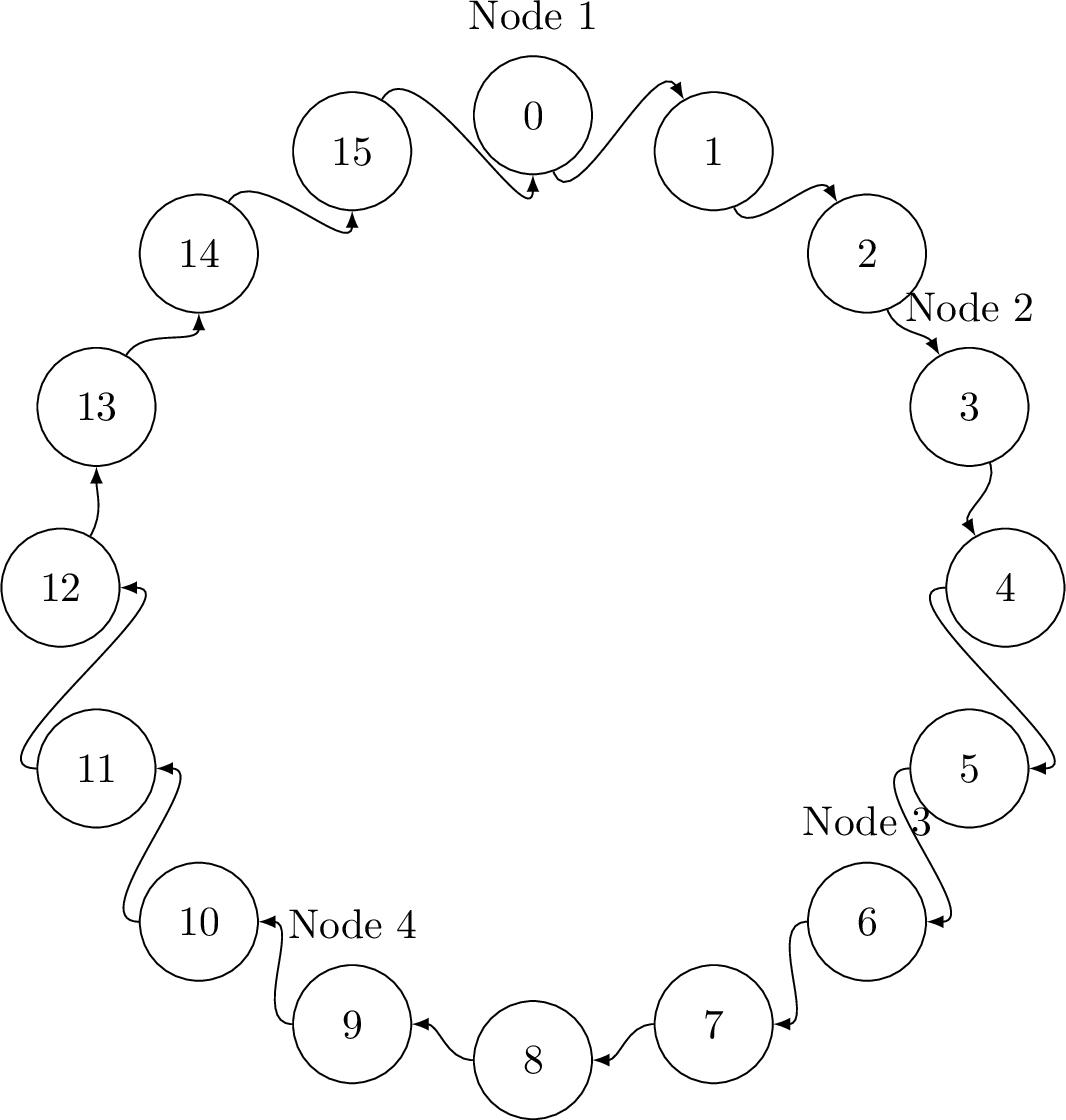
\includegraphics[width=0.45\textwidth]{fig/tex-grapics/chord.pdf.png}
  \caption{Chord Setup}
  \label{fig:chord}
\end{figure}

In diesem Beispiel sind die Knoten (Nodes) im Identifier-Raum wie folgt verteilt: Node 1: ID 0, Node 2: ID 3, Node 3: ID 6, Node 4: ID 9, Node 5: ID 13. Die Idee beim Chord Netz ist, dass der Knoten mit seiner zugeordneten ID verantwortlich ist für einen Bereich größer oder kleiner-gleich seiner eigenen ID. Dies würde für dieses Beispiel bedeuten, wenn der größer-gleich Bereich angenommen wird, dass Node 1 verantwortlich ist für die Keys 0-2, Node 2 verantwortlich für Key 3-5, Node 3 für 6-8, Node 4 für 9 -12 und Node 5 für 13-15. 

\begin{figure}[!ht]
  \centering
  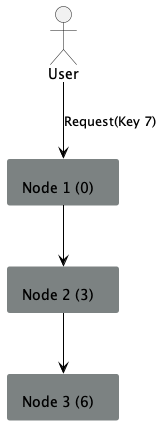
\includegraphics[width=0.15\textwidth]{fig/uml/chord.png}
  \caption{Chord Lookup Example ohne Fingertable}
  \label{fig:chord-lookup}
\end{figure}
Für das Auffinden der Nodes ohne Optimierung wie Fingertables ist nun eine lineare Suche über den Ring notwendig, der in der Graphik~\ref{fig:chord-lookup} beschrieben ist. Eine Suche (Lookup) für den Key 7 wird an dem Node 1 abgesetzt\footnote{Die Anfrage könnte auch an jeden anderen Knoten gestellt werden}. Node 1 ist nicht verantwortlich und leitet an Node 2 weiter, der sie schließlich an Node 3 weiterleitet. Node 3 ist für Key 7 zuständig und wird die angeforderte Ressource zurückgeben.
\\\\
Um den Suchaufwand zu reduzieren, kann zusätzlicher Aufwand für Strukturen betrieben werden, die wir als Fingertables bezeichnen. 
Fingertables sind ein zentraler Bestandteil der Chord-Architektur, die eine effiziente und schnelle Suche nach Schlüsseln und Knoten im Netzwerk ermöglichen. In einem Chord-Netzwerk speichert jeder Knoten eine Fingertable, die Informationen über andere Knoten im Netzwerk enthält. Die Fingertable besteht aus mehreren Einträgen, wobei jeder Eintrag auf einen \enquote{Finger} im Chord-Ring verweist. Die Funktionsweise von Fingertables kann wie folgt beschrieben werden:
\begin{itemize} 
\item Jede Fingertable hat genau $log(n)$ Einträge, wobei n die Anzahl der Knoten im Netzwerk ist.
\item Der i-te Eintrag in der Fingertable eines Knotens n verweist auf den ersten Knoten, der gleich oder nach $(n + 2^{(i-1)}) \mod 2^m$ liegt, wobei m die Anzahl der Bits für den Schlüsselraum ist (z. B. 160 für SHA-1) und i von 1 bis $log(n)$ reicht.
\item Fingertables ermöglichen eine schnelle Suche nach dem verantwortlichen Knoten für einen bestimmten Schlüssel, indem sie den Suchraum bei jedem Schritt effektiv halbieren. Dies wird erreicht, indem sie bei der Suche den nächstbesten Knoten wählen, der näher am gewünschten Schlüssel liegt.
\end{itemize} 

Damit die Fingertables wie erwartet funktionieren, muss sichergestellt werden, dass das Chord-Netzwerk  korrekt initialisiert ist, und alle Knoten müssen ihre Fingertables korrekt aufgebaut haben. Weiter müssen die Knoten im Netzwerk einvernehmliche und konsistente Informationen über die Schlüsselverteilung und die Positionen der anderen Knoten haben. Die Fingertables sollten regelmäßig aktualisiert werden, um Änderungen im Netzwerk - wie das Hinzufügen oder Entfernen von Knoten - zu berücksichtigen und sicherzustellen, dass die Routing-Informationen stets aktuell sind.

Die Verwendung ermöglicht eine effiziente Suche im Chord-Netzwerk, da sie den Suchraum bei jedem Schritt halbieren. Bei einem Lookup wird der am besten passende Knoten aus der Fingertabele ausgewählt, der näher am Ziel liegt, wodurch die Anzahl der Sprünge im Netzwerk verringert wird. Da die Fingertabele $log(n)$ Einträge hat, beträgt die maximale Anzahl der Sprünge, die benötigt werden, um einen Schlüssel zu finden, ebenfalls $log(n)$, dies auf die Hashfunktion zurückzuführen, die diese Verteilung sicherstellt. 
\\\\
Dies ist ein erheblicher Vorteil gegenüber einer naiven linearen Suche, bei der jeder Knoten einzeln überprüft werden müsste, bis der verantwortliche Knoten gefunden ist, was im schlimmsten Fall n Schritte erfordert.

\paragraph{Apache Cassandra Projekt\\\\}
Ein wichtiges Open Source Projekt, das auch der Chord Architektur basiert, ist das Apache Cassandra Projekt, welches hier kurz vorgestellt werden soll. Apache Cassandra ist ein verteiltes, hochverfügbares und skalierbares NoSQL-Datenbanksystem, das sich von der Chord-Architektur inspirieren ließ. Im Gegensatz zum klassischen Chord-Netzwerk hat Cassandra jedoch einige Anpassungen und Erweiterungen vorgenommen, um den Anforderungen moderner verteilter Datenbanksysteme gerecht zu werden. Durch dieses Projekt sollen einige Techniken eingeführt werden, die in der späteren Diskussion nochmal aufgenommen werden sollen. Weiter soll die Ausführung aufzeigen, wie bestehende Ideen über die Zeit Anpassungen und Optimierungen erfahren.

Einige der Anpassungen, die Apache Cassandra im Vergleich zur Chord-Architektur vorgenommen hat, sind:
\begin{itemize} 
\item Partitionierungsstrategie: In Cassandra werden Daten über mehrere Knoten (Nodes) verteilt, indem sie auf Basis eines Partitionsschlüssels, der aus den Eingabedaten extrahiert wird, partitioniert werden. Die Verantwortlichkeit für die Daten wird anhand eines konsistenten Hashing-Algorithmus, ähnlich wie bei Chord, bestimmt.

Die Hauptidee hinter Partitionierungsstrategien besteht darin, den Datenraum in kleinere Partitionen aufzuteilen und diese auf die verschiedenen Knoten im Cluster zu verteilen. Dadurch wird die Last gleichmäßiger auf die Knoten verteilt, und es wird verhindert, dass einige Knoten überlastet werden, während andere Knoten ungenutzt bleiben.

Cassandra verwendet einen Partitionsschlüssel, um den Platz einer Zeile innerhalb einer Tabelle zu bestimmen. Dieser Partitionsschlüssel wird durch einen Partitionierer, wie den Murmur3Partitioner, in einen Token-Wert konvertiert. Der Token-Wert wird dann verwendet, um den verantwortlichen Knoten für diese Partition zu bestimmen.

Sharding ist eine Partitionierungsstrategie, die in verteilten Datenbanksystemen verwendet wird, um Daten auf verschiedene Knoten oder Server aufzuteilen. So wird der gesamte Datensatz in kleinere, handhabbare Teile (Shards) aufgeteilt, wobei jeder Shard auf einem separaten Knoten oder Server gespeichert wird. Sharding kann auf verschiedene Arten implementiert werden, wie z.B.:
\begin{itemize} 
\item Range-based Sharding: Die Daten werden basierend auf einem bestimmten Wertebereich aufgeteilt. Zum Beispiel könnten Kundeninformationen basierend auf der Kunden-ID in unterschiedliche Shards aufgeteilt werden, wobei ein Shard Kunden-IDs von 1 bis 10.000, ein anderer Shard Kunden-IDs von 10.001 bis 20.000 usw. enthält.
\item Hash-based Sharding: Die Daten werden basierend auf einem Hash-Wert aufgeteilt, der aus dem Partitionsschlüssel berechnet wird. In diesem Fall wird der Hash-Wert verwendet, um die Daten gleichmäßig auf die verfügbaren Knoten zu verteilen.
\end{itemize}  
\item Replikationsstrategie: Um Datenverlust zu verhindern und hohe Verfügbarkeit zu gewährleisten, repliziert Cassandra Daten über mehrere Knoten hinweg. Die Anzahl der Replikationen und die Replikationsstrategie können konfiguriert werden. Im Gegensatz zum Chord-Netzwerk, das nur die direkten Nachfolgerknoten für die Replikation verwendet, unterstützt Cassandra verschiedene Replikationsstrategien wie SimpleStrategy und NetworkTopologyStrategy, um eine bessere Kontrolle über die Replikationslogik zu ermöglichen.
\item Datenmodell: Cassandra verwendet ein spaltenorientiertes Datenmodell, das sich von traditionellen relationalen Datenbanken unterscheidet. Das Datenmodell basiert auf einer Tabelle mit einer oder mehreren Partitionen, die wiederum aus einer oder mehreren Zeilen bestehen. Jede Zeile enthält einen eindeutigen Schlüssel und einen oder mehrere Spalten, die die Daten speichern.
\item Gossip-Protokoll: Im Gegensatz zur Chord-Architektur, die Fingertables für das Routing verwendet, verwendet Cassandra ein Gossip-Protokoll für die Kommunikation und den Informationsaustausch zwischen den Knoten. Das Gossip-Protokoll ermöglicht es Knoten, regelmäßig Informationen über ihren Status, ihre Last und die Topologie des Netzwerks auszutauschen.
\item Lese- und Schreibkonsistenz: Cassandra bietet die Möglichkeit, die Konsistenz von Lese- und Schreibvorgängen je nach Anforderungen der Anwendung anzupassen. Die Konsistenz kann auf unterschiedlichen Ebenen gewählt werden, von \enquote{One} (nur ein Knoten muss den Vorgang bestätigen) bis \enquote{All} (alle Replikationsknoten müssen den Vorgang bestätigen). Dies ermöglicht eine bessere Kontrolle über die Trade-offs zwischen Konsistenz, Verfügbarkeit und Performance.
\item Hinted Handoff: Cassandra verwendet ein Mechanismus namens \enquote{Hinted Handoff}, um vorübergehend ausgefallene Knoten zu behandeln. Wenn ein Knoten nicht verfügbar ist, um eine Schreiboperation durchzuführen, speichert ein anderer Knoten einen \enquote{Hint} und stellt die Daten dem ausgefallenen Knoten zur Verfügung, sobald dieser wieder online ist. Dieses Verfahren erhöht die Verfügbarkeit und Fehlertoleranz des Systems.
\item Repair und Anti-Entropy: Im Gegensatz zur Chord-Architektur verfügt Cassandra über Anti-Entropy- und Repair-Mechanismen, um Inkonsistenzen zwischen Replikationsknoten zu erkennen und zu beheben. Cassandra verwendet Merkle Trees, um Unterschiede zwischen Replikationen effizient zu erkennen und bei Bedarf Daten synchronisieren.
\end{itemize}
\paragraph{Anti-Entropy \\\\}
Anti-Entropy ist ein Mechanismus in verteilten Systemen, der dazu dient, die Konsistenz und Stabilität von Daten über mehrere Knoten (Nodes) hinweg sicherzustellen. In einem verteilten System arbeiten mehrere unabhängige Knoten zusammen, um eine gemeinsame Aufgabe zu erfüllen, wie zum Beispiel die Speicherung und Verwaltung von Daten. Diese Knoten können jedoch aufgrund von Netzwerkverzögerungen, Fehlern oder Abstürzen inkonsistente Daten enthalten. Diese Verfahren werden in einem späteren Kapitel nochmals genauer betrachtet. 
\\\\
Anti-Entropy-Prozesse sorgen dafür, dass die Daten auf den verschiedenen Knoten synchronisiert und konsistent bleiben. Sie verwenden Replikations- und Synchronisationsverfahren, um sicherzustellen, dass alle Knoten dieselben Daten enthalten,

%Termin-6 - vs-slides-chapter02-5

\newpage
% Work in progress

\section{Realisierung}
Bei der Implementierung von verteilten Systemen müssen mehrere Aspekte berücksichtigt werden, um sicherzustellen, dass das System effizient, zuverlässig und skalierbar ist. Eine umfassende Erörterung der Anforderungen in der Implementierung zu diskutieren ist aussichtslos, da eine nicht erfassbare Menge von Faktoren Einfluss haben. In den folgenden Punkten soll sich auf die grundsätzlichen Anforderungen an Prozesse und Kommunikation konzentriert werden. In den weiteren Kapiteln werden besondere Aspekte der Algorithmik, Koordination, Adressierung, wie auch Fehlertoleranz adressiert, bevor sich das Skript dem Testen und  dem Deployment zuwendet. 

\subsection{Prozesse und Threads}
Eine wesentliche Herausforderung ist die Organisation und die Strukturierung der Ablauffäden. Die kleinste, aus dem Modul Betriebssystemen, bekannte Struktur ist der Thread. Threads, implementiert auf einer node, bieten in verteilten Systemen mehrere Vorteile, die zu einer besseren Leistung, Ressourcennutzung und Reaktionsfähigkeit in einem verteilten System führen können:
\begin{itemize}
\item Parallelität: Threads ermöglichen die parallele Ausführung von Aufgaben innerhalb eines Prozesses, wodurch die Rechenressourcen (z.B. Mehrkernprozessoren) effizienter genutzt werden können. In verteilten Systemen kann dies dazu beitragen, dass mehrere Anfragen gleichzeitig auf einem Knoten verarbeitet werden, was zu einer schnelleren Reaktionszeit und einer besseren Leistung führt. Voraussetzung für die korrekte Einordnung des Mehrgewinns ist eine Unterscheidung in User- und Kernel-Threads.
\item Effiziente Ressourcennutzung: Da Threads innerhalb eines Prozesses ausgeführt werden, teilen sie sich den Speicher und andere Ressourcen. Dies ermöglicht eine effizientere Ressourcennutzung im Vergleich zur Verwendung von separaten Prozessen, die jeweils eigene Speicher- und Ressourcenbereiche haben. In verteilten Systemen kann dies dazu beitragen, den Gesamtressourcenverbrauch zu reduzieren. Hier liegt allerdings nicht der Fokus darauf die Threads über die gemeinsamen Ressourcen (z.B. Heap) zu koordinieren. Vielmehr verzichtet man vielmehr auf die Nutzung des gemeinsamen Speichers, um eine grundlegende Eigenschaft des verteilten Systems zu erhalten. Dies mag  im ersten Schritt merkwürdig klingen, erhält aber bei Einhaltung die Möglichkeit, die von den Threads umgesetzten Aufgaben auch auf Threads anderer Prozesse zu migrieren. Die Reduzierung liegt rein in der Reduzierung der Ressourcenverwwaltung, insbesondere auch dem Process Control Block.  

\item Reaktionsfähigkeit: Threads können unabhängig voneinander blockiert oder angehalten werden, während andere Threads im selben Prozess weiterlaufen. In verteilten Systemen kann dies dazu beitragen, die Reaktionsfähigkeit des Systems zu erhöhen, indem zeitaufwändige oder blockierende Aufgaben auf separate Threads ausgelagert werden, während andere Threads weiterhin Anfragen bedienen. Die Kontextwechsel sind im besten Fall leichter zu realisieren, als durch einen Prozess.

\item Granularität: Threads ermöglichen eine feinere Granularität bei der Parallelisierung von Aufgaben und können dazu beitragen, den Verwaltungsaufwand für die Verteilung von Aufgaben in verteilten Systemen zu reduzieren.
\end{itemize}
Trotz der Vorteile ist es wichtig, die Herausforderungen im Zusammenhang mit der Thread-Programmierung, wie z.B. Synchronisation, Deadlocks und Race Conditions, zu berücksichtigen und geeignete Techniken und Werkzeuge zur Bewältigung dieser Herausforderungen einzusetzen. Wichtig ist auch festzustellen, dass es für jede dieser Herausforderungen eine Lösung gibt, die aber verstanden und umgesetzt werden muss und jeweils mit negativen Eigenschaften belastet ist. Weiter kann auch auf besondere Eigenschaften der Threads verzichtet werden, um weiter die Defintion der verteilten Systemen zu erhalten um Mechanimsen, wie Skalierung, leichter zu etablieren.
\\\\
Die bereits angesprochene Abbildung der Threads im Betriebssystem ist weitere wesentliche Eigenschaft, die berücksichtigung finden muss. Es sollten hier zwei/drei Varianten unterschieden werden. Das \textbf{Many-to-One-Thread-Modell} ist ein Ansatz zur Verwaltung von Threads in einem Betriebssystem oder einer Anwendung, bei dem mehrere Benutzerthreads von einem einzigen Betriebssystem-Thread (\textbf{Kernel-Thread}) verwaltet werden. In diesem Modell werden die Benutzerthreads (\textbf{User-Threads})innerhalb der Anwendung geplant und ausgeführt, während der Kernel-Thread die Kommunikation und Interaktion mit dem Betriebssystem übernimmt. Vorteile und Nachteile des Many-to-One-Thread-Modells können wir beschreiben:
\begin{itemize}
\item Leichtgewicht: Da mehrere Benutzerthreads von einem einzigen Kernel-Thread verwaltet werden, sind die Ressourcenanforderungen für das System insgesamt geringer.
\item Portabilität: Da die Thread-Verwaltung auf Anwendungsebene erfolgt, ist das Many-to-One-Modell in der Regel unabhängig vom zugrunde liegenden Betriebssystem und daher portabeler zwischen verschiedenen Plattformen.
\item Skalierbarkeit: Da alle Benutzerthreads von einem einzigen Kernel-Thread verwaltet werden, kann das Modell nicht von Mehrkern- oder Mehrprozessorsystemen profitieren, da es keine echte Parallelität bietet.
\item Blockierung: Wenn ein Benutzerthread blockiert (z. B. aufgrund einer I/O-Operation), kann dies dazu führen, dass der gesamte Kernel-Thread blockiert wird und somit alle anderen Benutzerthreads zum Erliegen kommen.
\end{itemize}
Es existieren auch Alternativen zum Many-to-One-Thread-Modell, die wie folgt beschrieben werden können:
\begin{itemize}
\item \textbf{One-to-One-Thread-Modell}: In diesem Modell wird jedem Benutzerthread ein separater Kernel-Thread zugeordnet. Das One-to-One-Modell bietet bessere Skalierbarkeit und Parallelität, da mehrere Kernel-Threads gleichzeitig auf unterschiedlichen Kernen oder Prozessoren ausgeführt werden können. Allerdings kann es auch zu einer höheren Systembelastung führen, da mehr Ressourcen für die Verwaltung der Kernel-Threads benötigt werden.
\item \textbf{N:M-Thread-Modell} (auch bekannt als Many-to-Many-Thread-Modell): In diesem Modell gibt es eine variable Anzahl von Benutzerthreads und Kernel-Threads. Eine Gruppe von Benutzerthreads wird von einem oder mehreren Kernel-Threads verwaltet. Das N:M-Modell ermöglicht eine bessere Skalierbarkeit als das Many-to-One-Modell und kann bei der Ausnutzung von Mehrkern- oder Mehrprozessorsystemen effektiver sein. Es bietet auch eine gewisse Flexibilität bei der Zuordnung von Benutzerthreads zu Kernel-Threads, um den Anforderungen der Anwendung gerecht zu werden.
\end{itemize}
Jedes dieser Modelle hat seine Vor- und Nachteile. Die Wahl des am besten geeigneten Thread-Modells hängt von den Anforderungen der Anwendung, den verfügbaren Systemressourcen und der gewünschten Skalierbarkeit ab. Diese Aufzählung sollte auch primär der Auffrischung von Betriebssystemkenntnissen dienen. \\\\

\subsubsection{Threadpool}
Ein Threadpool ist ein Konzept in der Programmierung, bei dem eine bestimmte Anzahl von Threads im Voraus erstellt und verwaltet wird. Diese Threads werden zur parallelen Verarbeitung von Aufgaben in einer Warteschlange verwendet. Threadpools sind besonders nützlich, um die Systemressourcen effizient zu nutzen und die Leistung bei der Verarbeitung von vielen kleinen oder unabhängigen Aufgaben zu verbessern. Für parallele Aufgaben in einem homogenen und bekannten skalierenden System bietet dies ein breites Feld an Vorteilen. 
\begin{itemize}
\item Effiziente Ressourcennutzung: Da die Threads im Voraus erstellt und wiederverwendet werden, spart dies Zeit und Ressourcen, die sonst für das ständige Erstellen und Zerstören von Threads aufgewendet werden müssten.
\item Kontrolle über die Parallelität: Die Anzahl der Threads im Pool kann im Voraus festgelegt werden, um die Anzahl der gleichzeitig ausgeführten Aufgaben zu steuern und die Systemressourcen entsprechend zu nutzen.
\item Einfache Verwaltung: Ein Threadpool kümmert sich um die Verwaltung der Threads und die Zuweisung von Aufgaben, was die Komplexität bei der Verwaltung von Threads in der Anwendung reduziert.
\item Bessere Leistung: Threadpools können die Leistung verbessern, indem sie Wartezeiten reduzieren und die Reaktionsfähigkeit des Systems erhöhen.
\end{itemize}
Angenommen, es besteht eine Webanwendung, die eingehende Anfragen von Benutzern verarbeitet. Jede Anfrage kann unabhängig von den anderen bearbeitet werden und erfordert eine gewisse Rechenzeit. Anstatt für jede Anfrage einen neuen Thread zu erstellen, können Sie einen Threadpool verwenden. Hier ist ein einfaches Beispiel in Java, das einen Threadpool mit der ExecutorService-Klasse verwendet:\\\\

\begin{lstlisting}[caption={ExecutorService-Klasse},captionpos=b,label={lst:executor}]

import java.util.concurrent.ExecutorService;
import java.util.concurrent.Executors;

public class ThreadPoolExample {
    public static void main(String[] args) {
        int numThreads = 5;
        ExecutorService executor = Executors.newFixedThreadPool(numThreads);

        for (int i = 0; i < 10; i++) {
            Runnable task = new ExampleTask(i);
            executor.execute(task);
        }

        executor.shutdown();
    }
}

class ExampleTask implements Runnable {
    private int taskId;

    public ExampleTask(int taskId) {
        this.taskId = taskId;
    }

    @Override
    public void run() {
        System.out.println("Task " + taskId + " is running on thread: " + Thread.currentThread().getName());
    }
}
\end{lstlisting}
In diesem Beispiel erstellen wir einen Threadpool mit 5 Threads (numThreads). Der ExecutorService verwaltet den Threadpool und führt die ExampleTask-Instanzen aus. Da der Threadpool nur 5 Threads hat, werden maximal 5 Aufgaben (Tasks) gleichzeitig (im Zweifel nur Pseudoparallel) ausgeführt. Der ExecutorService sorgt dafür, dass alle Tasks in der Warteschlange abgearbeitet werden. Der Begriff des \textbf{Task} hat an dieser Stelle seinen Ursprung und findet in verteilten Systemen heute eine starke Nutzung.\\\\


Es gibt keine feste Regel für die maximale Auslastung eines Threadpools auf einer Node, da dies von der Anwendung und den Systemanforderungen abhängt. Ein allgemeiner Ansatz besteht darin, den Threadpool so zu konfigurieren, dass er die Anzahl der verfügbaren Prozessorkerne optimal nutzt. Als praktische Fausformel kann aber vielleicht mitgenommen werden, das ein Threadpool das gesamte System nicht mehr als 80 \% auslasten sollte.
Einige Empfehlungen für die Auslastung eines Threadpools auf einer Node sind:
\begin{itemize}
\item Berücksichtigen Sie die Art der Aufgaben, die der Threadpool ausführt. Bei rechenintensiven Aufgaben, die die CPU stark beanspruchen, ist es sinnvoll, die Anzahl der Threads auf die Anzahl der verfügbaren Prozessorkerne zu begrenzen. Bei Aufgaben, die auf I/O warten (z.B. Datei- oder Netzwerkzugriffe), kann es hilfreich sein, mehr Threads als Prozessorkerne zu verwenden, um die Wartezeiten besser auszugleichen.
\item Überwachen Sie die Systemauslastung und passen Sie die Größe des Threadpools bei Bedarf an. Wenn die CPU-Auslastung konstant hoch ist und die Anwendung langsamer wird, sollten Sie die Anzahl der Threads im Threadpool reduzieren. Wenn die CPU-Auslastung gering ist und viele Aufgaben auf I/O warten, können Sie die Anzahl der Threads im Threadpool erhöhen.
\end{itemize}
\paragraph{Task\\\\}

In verteilten Systemen bezieht sich der Begriff \enquote{Task} auf eine abstrakte Einheit von Arbeit oder eine Aufgabe, die von einem oder mehreren Komponenten innerhalb des Systems ausgeführt wird. Zur Wiederholung, ein verteiltes System besteht aus mehreren unabhängigen Rechnern oder Knoten, die zusammenarbeiten, um eine bestimmte Funktion oder einen bestimmten Prozess auszuführen. Wie festgestellt, ist das Worker-Thread-Pattern ein Entwurfsmuster, das häufig in verteilten Systemen verwendet wird, um die Verarbeitung von Tasks effizient zu handhaben. Ein gutes Design eines Tasks als Struktur zur Erfassung der Aufgabe sollte die folgenden Merkmale aufweisen:
\begin{itemize}
\item Modularität: Der Task sollte modular gestaltet sein, das heißt, er sollte in kleinere, unabhängige Einheiten zerlegt werden, die einzeln verarbeitet werden können. Dies ermöglicht eine einfachere Wiederverwendung von Code, erleichtert das Testen und ermöglicht es, das System bei Bedarf zu erweitern oder zu ändern.
\item Kapselung: Der Task sollte alle notwendigen Informationen und Ressourcen enthalten, um seine Arbeit auszuführen. Dies erleichtert das Verständnis der Task-Struktur, die Kommunikation zwischen den Systemkomponenten und die Fehlersuche im System.
\item Idempotenz: Wenn möglich, sollte der Task idempotent gestaltet sein, d.h. wenn er mehrmals mit den gleichen Eingaben ausgeführt wird, sollte er immer das gleiche Ergebnis liefern. Dies ist besonders wichtig in verteilten Systemen, in denen Fehler oder Netzwerkunterbrechungen dazu führen können, dass Tasks wiederholt oder neu gestartet werden müssen.
\item Zustandslosigkeit: Ein Task sollte zustandslos sein, das bedeutet, er sollte keine Informationen über frühere Ausführungen speichern. Zustandslose Tasks sind leichter zu verwalten und zu skalieren, da sie unabhängig voneinander auf verschiedenen Knoten ausgeführt werden können, ohne dass Informationen über den Zustand zwischen den Knoten synchronisiert werden müssen.
\item Fehlertoleranz: Der Task sollte so gestaltet sein, dass er bei Fehlern oder Ausfällen von Teilen des Systems weiterhin funktioniert. Dies kann durch Mechanismen wie Timeouts, Wiederholungsstrategien oder automatisches Failover erreicht werden.
\item Skalierbarkeit: Der Task sollte so gestaltet sein, dass er bei zunehmender Last oder Ressourcenanforderungen leicht skaliert werden kann. Das bedeutet, dass das System bei Bedarf einfach erweitert werden kann, indem zusätzliche Knoten oder Ressourcen hinzugefügt werden.
\item Kommunikation: Der Task sollte klar definierte Kommunikationsmechanismen und -protokolle verwenden, um Informationen zwischen den Systemkomponenten auszutauschen. Dies kann beispielsweise über Message Queues, Remote Procedure Calls (RPC) oder REST-APIs erfolgen.
\end{itemize}
Ein gut gestalteter Task bietet eine gute Grundlage für die Mechanismen der Skalierung. Hier sollte ausreichend Zeit in die Planung eingebracht werden.

\subsubsection{Multithreaded Clients}
In Multithreaded-Clients werden Threads häufig nicht nur zur Parallelisierung, sondern auch zur Organisation von Code und Aufgaben verwendet. Der Hauptgrund für diese Vorgehensweise ist, dass Multithreaded-Clients oft mit verschiedenen Arten von Aufgaben konfrontiert sind, die unabhängig voneinander und gleichzeitig ausgeführt werden müssen, um eine reibungslose Benutzererfahrung zu gewährleisten.
\\\\
Ein Webbrowser ist ein sehr gängiges Beispiel in diesem Kontext. Die Verwendung von Threads zur Organisation von Code und Aufgaben in solchen Fällen bietet mehrere Vorteile. Einige sollen beispielhaft diskutiert werden, die sich grundsätzlich über die Eigenschaften von Threads herleiten lassen:
\begin{itemize}
\item Reaktionsfähigkeit: Eine wichtige Anforderung für Client-Anwendungen ist, dass sie auf Benutzereingaben und Systemereignisse schnell reagieren können. Durch die Verwendung von Threads zur Organisation von Aufgaben können Benutzerinteraktionen und andere zeitkritische Prozesse unabhängig von zeitaufwändigen Hintergrundaufgaben (z. B. Dateioperationen, Netzwerkkommunikation) ausgeführt werden. Dies gewährleistet, dass die Anwendung auch während der Ausführung von langwierigen Aufgaben weiterhin reaktionsfähig bleibt.
\item Modularität und Wartbarkeit: Threads können verwendet werden, um Code und Aufgaben in logische, voneinander getrennte Einheiten zu organisieren. Dies verbessert die Lesbarkeit und Wartbarkeit des Codes, da jede Funktion oder Aufgabe innerhalb ihres eigenen Threads isoliert ist. Diese Modularität erleichtert auch das Debugging und die Fehlersuche in komplexen Anwendungen.
\item Bessere Ressourcennutzung: In einigen Fällen kann die Verwendung von Threads zur Organisation von Code und Aufgaben die Ressourcennutzung verbessern. Durch das Trennen von unabhängigen Aufgaben in separate Threads kann das System effizienter arbeiten, da es Ressourcen (z. B. Prozessorzeit) auf verschiedene Threads verteilt, anstatt sie einem einzigen, monolithischen Prozess zuzuweisen.
\item Vereinfachte Kommunikation: In Client-Anwendungen, die mit verschiedenen externen Diensten oder Datenquellen kommunizieren müssen, können Threads zur Organisation dieser Kommunikation verwendet werden. Indem jeder Kommunikationskanal in einem separaten Thread verwaltet wird, bleibt der Code für jeden Kanal sauber und leicht verständlich, während gleichzeitig das Risiko von Blockaden und Verzögerungen minimiert wird.
\end{itemize}
Ein einfaches Beispiel in Java, welches den Nutzen von Threads zur Organisation von Code und Aufgaben veranschaulicht, ist eine Anwendung, die eine Benutzerschnittstelle hat und gleichzeitig eine Datei herunterlädt. In diesem Beispiel bleiben die Benutzerschnittstelle und die Download-Aufgabe voneinander unabhängig, wodurch die Anwendung reaktionsfähig bleibt.\\\\
In diesem Beispiel des Listings~\ref{lst:down} wird ein separater Thread (downloadThread) erstellt, um den Download der Datei im Hintergrund durchzuführen. Während des Downloads kann der Hauptthread weiterhin Benutzereingaben über die Konsole akzeptieren und darauf reagieren, ohne von der Download-Aufgabe blockiert zu werden. Dies zeigt, wie Threads zur Organisation von Code und Aufgaben in einer Anwendung verwendet werden können, um eine bessere Reaktionsfähigkeit und Unabhängigkeit zwischen verschiedenen Aufgaben zu erreichen. Die Parallelisierung steht nicht immer im Vordergrund, obwohl die Erfassung nicht selten sinnvoll ist, dafür wird ein Maß eingeführt.

\paragraph{Thread-Level-Parallelism\\\\}
Thread-Level-Parallelism (TLP) ist ein Maß dafür, wie viele Threads in einer Anwendung gleichzeitig ausgeführt werden können. Eine Möglichkeit, TLP zu quantifizieren, besteht darin, den Speedup eines Programms zu berechnen, wenn es auf mehreren Threads parallel ausgeführt wird.\\\\

\noindent\begin{lstlisting}[caption={Threads zur Organisation},captionpos=b,label={lst:down}]
import java.io.BufferedInputStream;
import java.io.FileOutputStream;
import java.io.IOException;
import java.net.URL;
import java.util.Scanner;

public class DownloadExample {
    public static void main(String[] args) {
        Thread downloadThread = new Thread(() -> {
            System.out.println("Download-Thread gestartet");
            String fileUrl = "https://example.com/largefile.zip";
            String localFilename = "largefile.zip";

            try (BufferedInputStream in = new BufferedInputStream(new URL(fileUrl).openStream());
                 FileOutputStream fileOutputStream = new FileOutputStream(localFilename)) {
                byte[] dataBuffer = new byte[1024];
                int bytesRead;

                while ((bytesRead = in.read(dataBuffer, 0, 1024)) != -1) {
                    fileOutputStream.write(dataBuffer, 0, bytesRead);
                }
            } catch (IOException e) {
                e.printStackTrace();
            }

            System.out.println("Download abgeschlossen");
        });

        downloadThread.start();

        Scanner scanner = new Scanner(System.in);
        while (true) {
            System.out.println("Geben Sie 'exit' ein, um die Anwendung zu beenden");
            String input = scanner.nextLine();

            if (input.equalsIgnoreCase("exit")) {
                break;
            }

            System.out.println("Eingabe: " + input);
        }

        scanner.close();
    }
}
\end{lstlisting}

\begin{equation}
    Speedup = \frac{T_1}{T_p}
\end{equation}\\\\


Um TLP direkt zu berechnen, können wir den Speedup durch die Anzahl der Threads (p) teilen. Das Verhältnis gibt uns eine Idee davon, wie effektiv die parallele Ausführung auf mehreren Threads ist:

\begin{equation}
    TLP = \frac{Speedup}{p} = \frac{\frac{T_1}{T_p}}{p}
\end{equation}

Ein TLP von 1 würde bedeuten, dass das Programm perfekt parallelisiert ist, und jeder Thread gleichmäßig zur Reduzierung der Gesamtausführungszeit beiträgt. Ein TLP-Wert kleiner als 1 zeigt an, dass die parallele Ausführung weniger effektiv ist, da einige Threads möglicherweise auf Ressourcen warten oder es aufgrund von Synchronisationsproblemen zu Leistungsengpässen kommt.\\\\

Ein TLP von 1,5 bis 2 bedeutet, dass ein Webbrowser in der Lage ist, 1,5 bis 2 Threads gleichzeitig auszuführen, also einen Speedup unterstützt. Aber diese Zahl gibt auch an, dass ein Webbrowser nicht vollständig parallel ist. In diesem Beispiel können die Gründe dafür Vielfältig sein, Webbrowser müssen zahlreiche Aufgaben ausführen, wie das Laden und Darstellen von Webseiten, das Ausführen von JavaScript-Code, das Verarbeiten von Benutzereingaben und das Verwalten von Netzwerkanfragen. 
Webbrowser können somit eine gewisse Parallelität aufweisen, aber nicht extrem parallelisiert sein. Dies liegt daran, dass viele Aufgaben, die ein Browser ausführt, voneinander abhängig sind und eine gewisse Reihenfolge bei der Ausführung einhalten müssen. Zum Beispiel müssen HTML- und CSS-Ressourcen geladen und verarbeitet werden, bevor sie auf dem Bildschirm gerendert werden können, und JavaScript-Code kann die DOM-Struktur und das Erscheinungsbild einer Webseite verändern, was eine gewisse Synchronisation zwischen den Threads erfordert.
Ein TLP von 1,5 bis 2 bedeutet auch, dass Webbrowser die Ressourcen von modernen Multi-Core-Prozessoren nicht vollständig ausnutzen können. In vielen Fällen ist dies jedoch ausreichend, um eine gute Leistung und Benutzererfahrung zu gewährleisten.\\\\

Es ist wichtig zu beachten, dass der TLP-Wert von verschiedenen Faktoren abhängt, wie der Browserarchitektur, der verwendeten Webtechnologien und der Leistungsfähigkeit des zugrunde liegenden Systems. Daher kann der TLP-Wert für verschiedene Webbrowser und in verschiedenen Szenarien variieren.

\subsubsection{Single Threaded Process}
Ein Single-Threaded-Prozess ist ein Programm oder eine Anwendung, die nur einen einzigen Ausführungsstrang (Thread) verwendet, um Aufgaben nacheinander auszuführen. Dies steht im Gegensatz zu einem Multithreaded-Prozess, bei dem mehrere Threads parallel ausgeführt werden können, um gleichzeitig mehrere Aufgaben zu erledigen.

In einem Single-Threaded-Prozess werden die Aufgaben in einer sequenziellen Reihenfolge abgearbeitet, die durch den Programmfluss vorgegeben ist. Diese Art der Ausführung ist einfacher zu verstehen und zu programmieren, da keine Synchronisationsmechanismen oder Ressourcenschutzmaßnahmen erforderlich sind.\\\\

Ein Beispiel für die Umsetzung ist Node.js. Node.js ist eine serverseitige JavaScript-Laufzeitumgebung, die auf der V8-Engine von Google Chrome basiert. Eine der Hauptdesignphilosophien von Node.js ist die Verwendung eines Single-Threaded-Prozess, der asynchrone und ereignisgesteuerte I/O ermöglicht. Dies unterscheidet Node.js von vielen anderen serverseitigen Umgebungen, die auf Multithreading setzen, um mehrere gleichzeitige Anfragen zu verarbeiten. Der Single-Threaded-Prozess in Node.js bietet folgende Vorteile:
\begin{itemize}
\item Einfachheit: Da es nur einen Hauptthread gibt, entfallen die Probleme, die mit der Synchronisation von Threads, Deadlocks und Race Conditions verbunden sind. Dies vereinfacht den Programmieraufwand und reduziert die Wahrscheinlichkeit von schwer zu findenden Fehlern.
\item Skalierbarkeit: Node.js verwendet das ereignisgesteuerte Modell und asynchrone I/O-Aufrufe, um die Effizienz und Skalierbarkeit zu maximieren. Durch die Nichtblockierung von I/O-Aufrufen kann der Single-Threaded-Prozess eine große Anzahl gleichzeitiger Verbindungen effizient verwalten, ohne den Overhead, der durch das Erstellen und Verwalten mehrerer Threads entsteht.
\item Geringerer Ressourcenverbrauch: Da Node.js nur einen Thread verwendet, benötigt es weniger Systemressourcen wie Speicher und CPU im Vergleich zu serverseitigen Umgebungen, die mehrere Threads einsetzen. Dies kann insbesondere bei ressourcenbeschränkten Systemen von Vorteil sein. Es ist am Ende die einfachste Form einer Batch-Verarbeitung.
\end{itemize}
Ein einfaches Beispiel für einen Node.js-Server, der den Single-Threaded-Prozess verwendet, ist ein HTTP-Server, der Anfragen empfängt und verarbeitet:

\begin{lstlisting}[caption={Node.js Single Threaded},captionpos=b,label={lst:single}]
const http = require("http");
const server = http.createServer((req, res) => {
  console.log("Anfrage empfangen");

  // Simuliere eine zeitaufwaendige Operation
  setTimeout(() => {
    res.writeHead(200, { "Content-Type": "text/plain" });
    res.end("Hallo Welt!");
  }, 1000);
});
server.listen(3000, () => {
  console.log("Server laeuft auf Port 3000");
});
\end{lstlisting}
In diesem Beispiel erstellen wir einen einfachen HTTP-Server, der bei jeder Anfrage eine einsekündige Verzögerung simuliert. Da Node.js single-threaded ist, verwendet es asynchrone I/O-Aufrufe (in diesem Fall setTimeout), um die Verzögerung zu implementieren, ohne den Hauptthread zu blockieren. Während der Verzögerung kann der Hauptthread weiterhin neue Anfragen empfangen und verarbeiten.
\\\\
Acuh wenn der Single-Threaded-Prozess von Node.js in vielen Situationen Vorteile bietet, hat er auch seine Grenzen. Zum Beispiel kann der Single-Threaded-Prozess die Rechenleistung von Mehrkernprozessoren ohne weiteres nicht voll ausnutzen, und rechenintensive Aufgaben können die Leistungsfähigkeit des Servers beeinträchtigen. In solchen Fällen kann es sinnvoll sein, Techniken wie Clustering, Worker-Threads oder alternative Architekturen zu verwenden, um die Leistung und Skalierbarkeit der Anwendung zu verbessern.
\paragraph{Blocking vs non-blocking\\\\}
Parallelisierung und Blockierung (Blocking) sowie Nicht-Parallelisierung und Nicht-Blockierung (Non-blocking) sind zwei verschiedene Ansätze zur Programmierung und Systemgestaltung, die jeweils ihre eigenen Vor- und Nachteile haben, wobei die Non-Blocking Variante in Single-Threaded-Prozesse eine besondere Rolle haben, da sie viele Vorteile hat. 
\begin{itemize}
\item Höhere Skalierbarkeit: Non-Blocking I/O ermöglicht es, mehr gleichzeitige Verbindungen oder Anfragen mit weniger Ressourcen (z.B. Threads oder Prozesse) zu verwalten, was zu einer besseren Skalierbarkeit führt.
\item Bessere Leistung: Da Non-Blocking I/O Threads oder Prozesse nicht blockiert, können diese Ressourcen für andere Aufgaben verwendet werden, wodurch die Gesamtleistung des Systems verbessert wird.
\item Reduzierte Latenz: Non-Blocking I/O ermöglicht es, dass mehrere I/O-Operationen gleichzeitig ausgeführt werden, wodurch die Gesamtlatenz für das Abschließen einer Gruppe von Operationen reduziert wird.
\end{itemize}
Non-Blocking I/O-Techniken werden häufig in serverseitigen Anwendungen wie Webservern, Datenbanken und anderen Netzwerkdiensten eingesetzt, um eine höhere Skalierbarkeit und bessere Leistung zu erzielen. Es gibt verschiedene Ansätze, um Non-Blocking I/O im Netzwerkbereich zu implementieren:
\begin{itemize}
\item Asynchrone I/O (AIO): Asynchrone I/O-Operationen ermöglichen es, dass ein Thread oder Prozess eine I/O-Operation startet und sofort zur nächsten Anweisung übergeht, ohne auf das Ergebnis der Operation zu warten. Das Betriebssystem benachrichtigt den Thread oder Prozess, wenn die I/O-Operation abgeschlossen ist, normalerweise über Callback-Funktionen oder Ereignisse.
\item I/O-Multiplexing (auch bekannt als Event-Driven I/O): Bei dieser Technik wird ein zentrales Ereignishandling-System verwendet, um auf mehrere I/O-Operationen gleichzeitig zu warten und das Programm über abgeschlossene Operationen zu informieren. Beispiele für I/O-Multiplexing-APIs sind select, poll und epoll in Unix/Linux-Systemen.
\item Non-Blocking Sockets: Dieser Ansatz verwendet spezielle Socket-Optionen, um Netzwerkoperationen wie send und recv in einem Nicht-Blockiermodus auszuführen. Auch wenn die Operation nicht sofort abgeschlossen werden kann, gibt die Funktion sofort zurück und zeigt an, dass die Operation später erneut versucht werden sollte.
\end{itemize}
Trotz der Vorteile sollte verstanden sein, dass die Programmierung von Non-Blocking I/O im Netzwerkbereich komplexer sein wird, als die Verwendung von blockierenden I/O-Operationen, da Entwickler zusätzliche Mechanismen für das Ereignishandling und die Synchronisation implementieren müssen.
\\\\
Ein Beispiel für Non-Blocking I/O ist in Java die Verwendung von java.nio-Paketen, welche asynchrone und Non-Blocking I/O-Operationen unterstützen. In diesem Beispiel erstellen wir einen einfachen Echo-Server, der Non-Blocking I/O mit java.nio.channels verwendet:

\begin{lstlisting}[caption={Non-Blocking},captionpos=b,label={lst:nonb}]
import java.io.IOException;
import java.net.InetSocketAddress;
import java.nio.ByteBuffer;
import java.nio.channels.SelectionKey;
import java.nio.channels.Selector;
import java.nio.channels.ServerSocketChannel;
import java.nio.channels.SocketChannel;
import java.util.Iterator;
import java.util.Set;

public class NonBlockingEchoServer {
    public static void main(String[] args) throws IOException {
        // Create a new selector
        Selector selector = Selector.open();

        // Create a new server socket channel and bind it to a port
        ServerSocketChannel serverSocketChannel = ServerSocketChannel.open();
        serverSocketChannel.bind(new InetSocketAddress(8000));

        // Configure the server socket channel to be non-blocking
        serverSocketChannel.configureBlocking(false);

        // Register the server socket channel with the selector for accepting new connections
        serverSocketChannel.register(selector, SelectionKey.OP_ACCEPT);

        while (true) {
            // Wait for events
            int readyChannels = selector.select();

            if (readyChannels == 0) {
                continue;
            }

            Set<SelectionKey> selectedKeys = selector.selectedKeys();
            Iterator<SelectionKey> keyIterator = selectedKeys.iterator();

            while (keyIterator.hasNext()) {
                SelectionKey key = keyIterator.next();

                if (key.isAcceptable()) {
                    // Accept the new connection
                    ServerSocketChannel serverChannel = (ServerSocketChannel) key.channel();
                    SocketChannel socketChannel = serverChannel.accept();

                    // Configure the new socket channel to be non-blocking
                    socketChannel.configureBlocking(false);

                    // Register the new socket channel with the selector for reading data
                    socketChannel.register(selector, SelectionKey.OP_READ);
                } else if (key.isReadable()) {
                    // Read the data from the socket channel
                    SocketChannel socketChannel = (SocketChannel) key.channel();
                    ByteBuffer buffer = ByteBuffer.allocate(256);
                    int bytesRead = socketChannel.read(buffer);

                    if (bytesRead == -1) {
                        // Close the socket channel if the client has disconnected
                        socketChannel.close();
                    } else {
                        // Echo the data back to the client
                        buffer.flip();
                        socketChannel.write(buffer);
                    }
                }

                keyIterator.remove();
            }
        }
    }
}
\end{lstlisting}
Das Listing~\ref{lst:nonb} seigt einen Selector, um gleichzeitig mehrere Verbindungen zu verwalten. Der Echo-Server liest Daten von verbundenen Clients und sendet die empfangenen Daten sofort an den jeweiligen Client zurück.

\subsubsection{Serveranwendungen}
Bei der Entwicklung von Serveranwendungen kann die Architektur entweder auf einem iterativen (sequentiellen) oder einem nebenläufigen (Concurrent) Ansatz basieren. Beide Ansätze haben ihre eigenen Vor- und Nachteile, abhängig von den Anforderungen der Anwendung und den zugrunde liegenden Systemressourcen. 

Ein \textbf{iterativer Server} verarbeitet Anfragen sequenziell, d.h. er verarbeitet eine Anfrage vollständig, bevor er zur nächsten übergeht.  Durch die Verwendung des iterativen Servers ergeben sich Vorteile wie Nachteile:
\begin{itemize}
\item Einfache Implementierung: Iterative Server sind einfacher zu entwickeln und zu warten, da sie keine komplexen nebenläufigen Programmierkonzepte erfordern. Es müssen keine Nebenläufigkeitsprobleme, wie Synchronisation, Deadlocks oder Race Conditions, berücksichtigt werden.
\item Geringerer Ressourcenverbrauch: Da keine zusätzlichen Threads oder Prozesse erstellt werden, verbraucht ein iterativer Server in der Regel weniger Ressourcen wie Speicher und CPU.
\item Skalierbarkeit: Da ein iterativer Server Anfragen sequenziell verarbeitet, kann er bei einer großen Anzahl gleichzeitiger Anfragen schnell überlastet werden und zu einer schlechten Leistung führen. Das Warteschlangen-Modell kann auch hier Antworten bieten.
\item Reaktionsfähigkeit: Wenn eine Anfrage zeitaufwändige oder blockierende Operationen beinhaltet, werden nachfolgende Anfragen verzögert, was zu einer schlechteren Benutzererfahrung führen kann.
\end{itemize}
Ein \textbf{nebenläufiger Server} verwendet Threads oder Prozesse, um mehrere Anfragen gleichzeitig zu verarbeiten. Dadurch kann der Server eine größere Anzahl von Anfragen effizienter verarbeiten und eine bessere Reaktionsfähigkeit bieten. Auch Concurrent Server haben Vorteile wie Nachteile:

\begin{itemize}
\item Skalierbarkeit: Durch die Verwendung von Threads oder Prozessen zur gleichzeitigen Verarbeitung von Anfragen kann ein nebenläufiger Server eine größere Anzahl gleichzeitiger Verbindungen bewältigen und eine bessere Leistung bieten.
\item Reaktionsfähigkeit: Da jeder Thread oder Prozess unabhängig von den anderen arbeitet, können nebenläufige Server auch bei zeitaufwändigen oder blockierenden Operationen eine bessere Reaktionsfähigkeit bieten.
\item Komplexität: Die Implementierung eines nebenläufigen Servers erfordert ein besseres Verständnis von nebenläufigen Programmierkonzepten wie Synchronisation, Deadlocks und Race Conditions. Dies kann zu einer komplexeren und fehleranfälligeren Implementierung führen.
\end{itemize}
Die Wahl zwischen einem iterativen und einem nebenläufigen Server hängt von den Anforderungen der Anwendung und den Ressourcen des Systems ab. Für Anwendungen mit geringem Verkehrsaufkommen und einfachen Anforderungen kann ein iterativer Server ausreichend sein. Hier sind zwei einfache Beispiele in Listing~\ref{lst:iterativ} und Listing~\ref{lst:concurrent} für einen iterativen und einen nebenläufigen Server in Java unter Verwendung des java.net-Pakets:
\begin{lstlisting}[caption={Iterativer Server},captionpos=b,label={lst:iterativ}]
import java.io.IOException;
import java.io.InputStream;
import java.io.OutputStream;
import java.net.ServerSocket;
import java.net.Socket;

public class IterativeServer {
    public static void main(String[] args) throws IOException {
        int port = 1234;
        ServerSocket serverSocket = new ServerSocket(port);

        while (true) {
            Socket clientSocket = serverSocket.accept();
            handleClient(clientSocket);
            clientSocket.close();
        }
    }

    public static void handleClient(Socket clientSocket) throws IOException {
        InputStream input = clientSocket.getInputStream();
        byte[] buffer = new byte[1024];
        int bytesRead = input.read(buffer);
        System.out.println("Received: " + new String(buffer, 0, bytesRead));

        OutputStream output = clientSocket.getOutputStream();
        output.write("Hello, Client!".getBytes());
    }
}
\end{lstlisting}
In dem Listing des iterativen Serves erkennen wir einen einfachen Echo-Server, der die vom Client gesendeten Nachrichten empfängt und eine Antwort zurücksendet. Der iterative Server verarbeitet die Anfragen nacheinander, während der nebenläufige Server in Listing~\ref{lst:concurrent} für jede Anfrage einen neuen Thread erstellt, um sie gleichzeitig zu verarbeiten, dies ist im folgenden Beispiel erkennbar.

\begin{lstlisting}[caption={Concurrent Server},captionpos=b,label={lst:concurrent}]
import java.io.IOException;
import java.io.InputStream;
import java.io.OutputStream;
import java.net.ServerSocket;
import java.net.Socket;

public class ConcurrentServer {
    public static void main(String[] args) throws IOException {
        int port = 1234;
        ServerSocket serverSocket = new ServerSocket(port);

        while (true) {
            Socket clientSocket = serverSocket.accept();
            new Thread(() -> {
                try {
                    handleClient(clientSocket);
                } catch (IOException e) {
                    e.printStackTrace();
                } finally {
                    try {
                        clientSocket.close();
                    } catch (IOException ex) {
                        ex.printStackTrace();
                    }
                }
            }).start();
        }
    }

    public static void handleClient(Socket clientSocket) throws IOException {
        InputStream input = clientSocket.getInputStream();
        byte[] buffer = new byte[1024];
        int bytesRead = input.read(buffer);
        System.out.println("Received: " + new String(buffer, 0, bytesRead));

        OutputStream output = clientSocket.getOutputStream();
        output.write("Hello, Client!".getBytes());
    }
}
\end{lstlisting}

\subsubsection{Prozesse}

In verteilten Systemen spielen Prozesse eine entscheidende Rolle für die Organisation und Durchführung von Aufgaben. Im Kontext von verteilten Systemen bezieht sich der Begriff \enquote{Prozess} häufig auf einen laufenden Task oder eine Anwendung, die auf einem der Knoten im System ausgeführt wird oder, in einer groberen Granularität, einen Dienst (Service). In verteilten Systemen können mehrere Prozesse gleichzeitig auf verschiedenen Knoten (nodes) ausgeführt werden, um die Leistung und Effizienz des Systems zu steigern. Dies ermöglicht eine schnellere Verarbeitung von Aufgaben und eine bessere Auslastung der Ressourcen. 
Die Möglichkeit, Prozesse auf verschiedenen Knoten auszuführen, ermöglicht es verteilten Systemen, die Last auf die verfügbaren Ressourcen zu verteilen und bei Bedarf zu skalieren. Wenn die Systemlast zunimmt, können zusätzliche Knoten hinzugefügt werden, um die Leistung zu erhöhen und die Ausführung der Prozesse zu beschleunigen. Prozesse in verteilten Systemen können so konzipiert sein, dass sie bei Ausfällen oder Fehlern in anderen Teilen des Systems weiterhin funktionieren (Fehlertolerant). Dies kann durch redundante Prozesse, Replikation oder automatisches Failover erreicht werden. Diese Techniken werden im Folgenden noch besprochen. Ein weiterer Vorteil ist, Prozesse können unabhängig voneinander entwickelt, getestet und gewartet werden. Dies erleichtert die Implementierung von Änderungen und die Isolierung von Fehlern. \\\\

Eine wesentliche Herausforderung ist, dass in verteilten Systemen Prozesse miteinander kommunizieren müssen, um Informationen auszutauschen. Die Kommunikation zwischen Prozessen kann über verschiedene Mechanismen erfolgen, wie z. B. Message Passing, Remote Procedure Calls (RPC) oder REST-APIs. Grundlage ist aber meist die Interprocess-Kommunikation (IPC).
Neben der Kommunikation ist aber auch die Portierung der Prozesse auf verschiedene Orte eine besondere Herausforderung, auch um die Verteilungstransparenz und die Skalierung über die Problemgröße zu erreichen. \\\\
Selbst beterogene Systeme bestehen aus unterschiedlichen Hardware- und Softwarekomponenten, wie z. B. verschiedene Prozessorarchitekturen, Betriebssysteme oder Netzwerkprotokolle. Diese Unterschiede können zu Problemen bei der Portierung führen, darunter aus anderen Modulen bekannte Probleme:
\begin{itemize}
\item Unterschiedliche Prozessorarchitekturen: Verschiedene Systeme können unterschiedliche Prozessortypen verwenden (z. B. x86, ARM, MIPS), die jeweils eigene Befehlssätze und Spezifikationen haben. Bei der Portierung von Prozessen müssen diese Unterschiede berücksichtigt werden, und der Code muss möglicherweise angepasst oder neu kompiliert werden, um auf der Zielplattform korrekt zu funktionieren.
\item Betriebssystemabhängigkeiten: Prozesse können Funktionen oder APIs verwenden, die spezifisch für ein bestimmtes Betriebssystem sind. Bei der Portierung auf ein anderes Betriebssystem müssen diese Abhängigkeiten identifiziert und angepasst werden, um Inkompatibilitäten zu vermeiden.
\item Byte-Reihenfolge (Endianess): Unterschiedliche Systeme können unterschiedliche Byte-Reihenfolgen verwenden (Big-Endian oder Little-Endian). Dies kann zu Problemen bei der Interpretation von Daten führen, die zwischen Systemen ausgetauscht werden. Bei der Portierung von Prozessen muss die Byte-Reihenfolge berücksichtigt und möglicherweise konvertiert werden, um eine korrekte Kommunikation und Datenverarbeitung zu gewährleisten.
\item Speicherverwaltung: Verschiedene Systeme können unterschiedliche Speicherverwaltungsmechanismen verwenden, z. B. hinsichtlich der Speicherzuweisung, Freigabe oder Adressierung. Bei der Portierung von Prozessen müssen diese Unterschiede berücksichtigt werden, und der Code muss möglicherweise angepasst werden, um auf der Zielplattform korrekt zu funktionieren.
\item Kommunikationsprotokolle: In heterogenen Systemen können unterschiedliche Kommunikationsprotokolle oder Netzwerkstandards zum Einsatz kommen. Bei der Portierung von Prozessen müssen diese Unterschiede berücksichtigt werden, und es müssen möglicherweise Anpassungen an der Kommunikationsschnittstelle vorgenommen werden, um eine korrekte Interaktion zwischen den Komponenten zu ermöglichen.
\item Leistungsunterschiede: Unterschiedliche Hardwarekomponenten in heterogenen Systemen können zu unterschiedlichen Leistungsniveaus führen. Bei der Portierung von Prozessen sollten diese Unterschiede berücksichtigt werden, um sicherzustellen, dass die Anwendung auf der Zielplattform effizient und performant arbeitet.
\item Softwarebibliotheken und Frameworks: Prozesse können von externen Softwarebibliotheken oder Frameworks abhängig sein, die möglicherweise nicht auf der Zielplattform verfügbar sind oder unterschiedliche Versionen aufweisen. Bei der Portierung müssen solche Abhängigkeiten identifiziert und angepasst werden, um Inkompatibilitäten zu vermeiden.
\end{itemize}
Um die Portierung von Prozessen auf heterogenen Systemen erfolgreich durchzuführen, sind einige Strategien und Techniken hilfreich:
\begin{itemize}
\item Abstraktion: Verwenden Sie Abstraktionsschichten, um plattformspezifische Details zu kapseln und einen gemeinsamen Satz von Schnittstellen für die Anwendung bereitzustellen. Dadurch wird die Portierung erleichtert, da nur die plattformspezifischen Implementierungsdetails angepasst werden müssen.
\item Plattformunabhängige Programmiersprachen und Laufzeitumgebungen: Verwenden Sie plattformunabhängige Programmiersprachen (z. B. Java, Python) oder Laufzeitumgebungen (z. B. .NET Core), die auf verschiedenen Plattformen ausgeführt werden können. Diese Technologien ermöglichen es, den Code einmal zu schreiben und auf mehreren Plattformen auszuführen, was die Portierungsaufwände reduziert.
\item Standardbibliotheken und Protokolle: Nutzen Sie standardisierte Bibliotheken, Frameworks und Kommunikationsprotokolle, die auf verschiedenen Plattformen verfügbar und kompatibel sind. Dies erleichtert die Portierung, da die Abhängigkeiten und Schnittstellen zwischen den Systemkomponenten konsistent bleiben.
\item Cross-Kompilierung: Verwenden Sie Cross-Kompiler, um den Code für verschiedene Zielplattformen zu kompilieren. Dies ermöglicht eine bessere Kontrolle über die Erstellung von Binärdateien, die auf verschiedenen Prozessorarchitekturen ausgeführt werden können.
\item Automatisiertes Testen: Stellen Sie sicher, dass Sie umfangreiche Testsuiten haben, die alle wichtigen Funktionen Ihrer Anwendung abdecken. Automatisierte Tests sind besonders wichtig bei der Portierung von Prozessen, da sie dabei helfen, Fehler und Inkompatibilitäten schnell zu erkennen und zu beheben.
\item Dokumentation und Wissenstransfer: Eine gute Dokumentation der Anwendung, der verwendeten Technologien und der plattformspezifischen Details ist entscheidend für den Erfolg der Portierung. Der Wissenstransfer zwischen den Entwicklern, die an der Portierung beteiligt sind, hilft dabei, mögliche Probleme zu identifizieren und effizient zu lösen.
\end{itemize}
Indem diese Strategien und Techniken angewendet werden, können die Herausforderungen bei der Portierung von Prozessen auf heterogenen Systemen besser bewältigt werden, und die Wahrscheinlichkeit eines erfolgreichen Portierungsprojekts wird erhöht. Aber auch wenn selbst die Portierung und die Etablierung auf singulärer Hardware ausreicht, sind weitere Herausforderungen zu berücksichtigen. Beispielhaft, wenn mehrere Prozesse auf derselben Hardware ausgeführt werden, können Isolations- und Sicherheitsprobleme auftreten. Einige der häufigsten Probleme sind:
\begin{itemize}
\item Speicherzugriffsverletzungen: Wenn Prozesse auf demselben System ausgeführt werden, besteht das Risiko, dass sie auf den Speicherbereich eines anderen Prozesses zugreifen und somit Daten beschädigen oder korrumpieren. Moderne Betriebssysteme implementieren Speicherschutzmechanismen, um den Speicherbereich jedes Prozesses voneinander zu isolieren. Dennoch kann es aufgrund von Fehlern oder Schwachstellen in der Software zu unerwünschten Speicherzugriffen kommen.
\item Ressourcenkonflikte: Mehrere Prozesse, die auf derselben Hardware laufen, müssen sich die verfügbaren Ressourcen teilen, wie z. B. CPU, Speicher, I/O-Geräte und Netzwerkbandbreite. Ressourcenkonflikte können zu Leistungseinbußen, unvorhersehbarem Verhalten oder Systeminstabilität führen.
\item Nebenkanalangriffe: Bei Nebenkanalangriffen nutzt ein Angreifer Informationen, die durch die Ausführung von Prozessen auf derselben Hardware unbeabsichtigt preisgegeben werden, um vertrauliche Daten abzuleiten. Beispiele sind Cache-Timing-Angriffe oder die Spectre- und Meltdown-Schwachstellen, die aufgrund von Hardware-Designfehlern in modernen Prozessoren entstanden sind.
\item Privilegienerweiterung: Ein Prozess, der in der Lage ist, höhere Berechtigungen oder Systemressourcen zu erlangen, als ihm ursprünglich zugewiesen wurden, kann die Sicherheit und Isolation anderer Prozesse gefährden. Ein Angreifer kann solche Schwachstellen ausnutzen, um auf vertrauliche Daten zuzugreifen oder die Kontrolle über das System zu erlangen.
\item Prozess-Interaktionen: Wenn Prozesse auf demselben System interagieren, etwa über Interprozesskommunikation (IPC) oder gemeinsam genutzte Ressourcen, kann dies Sicherheitsrisiken bergen. Ein Angreifer kann versuchen, solche Interaktionen zu manipulieren, um Daten abzufangen oder Prozesse zu beeinflussen.
\end{itemize}
Um die Isolation und Sicherheit von Prozessen auf derselben Hardware zu gewährleisten, können verschiedene Maßnahmen ergriffen werden:
\begin{itemize}
\item Zugriffskontrolle: Implementierung strenger Zugriffskontrollmechanismen, um sicherzustellen, dass Prozesse nur auf die Ressourcen zugreifen können, die sie benötigen.
\item Sandboxen: Prozesse werden in isolierten Umgebungen ausgeführt, z. B. in Containern oder virtuellen Maschinen, um die Isolation zwischen Prozessen zu verbessern und die Angriffsfläche zu reduzieren.
\item Überwachung und Auditing: Überwachung der Aktivitäten von Prozessen, um verdächtiges Verhalten oder Sicherheitsverletzungen frühzeitig zu erkennen.
\item Sicherheitspatches: Betriebssystem und die Anwendungssoftware auf dem neuesten Stand halten, indem regelmäßig Sicherheitspatches und Updates installiert werden. Dies hilft, bekannte Schwachstellen zu beheben, die von Angreifern ausgenutzt werden könnten.
\item Prinzip der geringsten Privilegien: Prozesse nur die minimal erforderlichen Berechtigungen zuweisen. Dies reduziert das Risiko von Privilegienerweiterungsangriffen und minimiert die potenziellen Schäden, die ein kompromittierter Prozess verursachen kann.
\item Kryptografie: Nutzung von kryptografische Verfahren, um vertrauliche Daten in Speicher und während der Übertragung zu schützen. Dies verhindert, dass Angreifer auf sensible Informationen zugreifen können, selbst wenn sie Zugang zu einem kompromittierten Prozess erhalten.
\item Prozess-Isolation auf Hardware-Ebene: Einige Prozessoren und Plattformen bieten Hardware-unterstützte Funktionen zur Isolation von Prozessen, wie z. B. Intel's Software Guard Extensions (SGX) oder ARM's TrustZone. Durch die Nutzung dieser Funktionen kann die Isolation und Sicherheit von Prozessen auf derselben Hardware verbessert werden.
\item Sicherheitsbewusstes Design und Entwicklung: Sicherheit von Anfang an in den Entwicklungsprozess integrieren. Verwendung sicherer Programmierpraktiken und Durchführung regelmäßiger Sicherheitsanalysen und -prüfungen durch, um Schwachstellen frühzeitig zu identifizieren und zu beheben.
\end{itemize}
Indem diese Maßnahmen umgesetzt werden, können die Isolation und Sicherheit verbessert und potenzielle Sicherheitsrisiken minimiert werden. Es ist wichtig, einen mehrschichtigen Sicherheitsansatz zu verfolgen und auf allen Ebenen des Systems für eine robuste Verteidigung zu sorgen.

\subsubsection{Prozessverwaltung}
Distributed Operating Systems (DOS) und Network Operating Systems (NOS) sind zwei Ansätze zur Verwaltung von Prozessen in verteilten Systemen. Hier ist zunächst ein Überblick über die Hauptmerkmale von DOS, gefolgt von einem Beispiel aus der Praxis:
\begin{itemize}
\item Transparenz: DOS zielt darauf ab, die Verteilung der Ressourcen und Prozesse im System weitgehend zu verbergen. Das bedeutet, dass die Benutzer und Anwendungen das verteilte System als einen einzigen, kohärenten Computer wahrnehmen, obwohl es aus mehreren, vernetzten Knoten besteht.
\item Globale Ressourcenverwaltung: In einem DOS werden Ressourcen wie Speicher, Prozessorleistung und I/O-Geräte zentral verwaltet und den Prozessen im System zugewiesen. Dies ermöglicht eine effiziente Nutzung der verfügbaren Ressourcen und fördert Lastverteilung und Fehlertoleranz.
\item Prozessmigration: DOS ermöglicht die Migration von Prozessen zwischen verschiedenen Knoten im verteilten System. Dies kann dazu beitragen, die Ausführungsgeschwindigkeit zu verbessern, die Last im System auszugleichen oder die Verfügbarkeit von Anwendungen zu erhöhen.
\item Kommunikation: DOS stellt integrierte Kommunikationsmechanismen zur Verfügung, die es Prozessen ermöglichen, miteinander zu kommunizieren und auf verteilte Ressourcen zuzugreifen. Diese Mechanismen sind in das Betriebssystem eingebettet und bieten eine hohe Abstraktionsebene, um die Entwicklung von verteilten Anwendungen zu erleichtern.
\end{itemize}
Mesosphere, besser bekannt als das Datacenter Operating System (DC/OS)\footnote{\url{https://dcos.io/}}, kann als Beispiel für ein modernes Distributed Operating System (DOS) angesehen werden. Das Produkt DC/OS basiert weiter auf Apache Mesos, einem Cluster-Manager und Ressourcen-Orchestrierungs-Framework.
\\\\
DC/OS ist darauf ausgelegt, Ressourcen in einem verteilten System oder Rechenzentrum effizient zu verwalten und Anwendungen über mehrere Knoten hinweg zu betreiben. Es stellt Funktionen wie Ressourcenmanagement, Prozessverwaltung, Lastverteilung und Fehlertoleranz für Anwendungen bereit, die auf verteilten Knoten im Rechenzentrum laufen. Ein Beispiel für ein  älteres Distributed Operating System (DOS) ist Amoeba. Amoeba wurde in den 1980er und 1990er Jahren an der Vrije Universiteit in Amsterdam von Andrew S. Tanenbaum entwickelt und zeigt viele Basis-Elemente heutiger Architekturen für DOS auf. 
\\\\
Network Operating Systems (NOS) werden hauptsächlich in Umgebungen eingesetzt, in denen die Zusammenarbeit, gemeinsame Nutzung von Ressourcen und Kommunikation zwischen Computern und Benutzern im Vordergrund steht und ist mit folgenden Hauptmerkmalen belegt: 
\begin{itemize}
\item Verteilte Ressourcenverwaltung: Im Gegensatz zu DOS verwaltet NOS die Ressourcen dezentral auf jedem Knoten im Netzwerk. Jeder Knoten führt ein eigenes Betriebssystem aus und verwaltet seine eigenen Ressourcen, wie z.B. Speicher, Prozessorleistung und I/O-Geräte.
\item Datei- und Ressourcenteilung: NOS konzentriert sich darauf, Ressourcen wie Dateien, Drucker oder Anwendungen über das Netzwerk gemeinsam zu nutzen. Benutzer und Anwendungen können auf diese Ressourcen zugreifen, die auf verschiedenen Knoten im Netzwerk verfügbar sind.
\item Netzwerkprotokolle: NOS verwendet standardisierte Netzwerkprotokolle wie TCP/IP, um die Kommunikation und den Austausch von Daten zwischen den Knoten im Netzwerk zu ermöglichen.
\item Skalierbarkeit: Da jeder Knoten seine eigenen Ressourcen verwaltet, kann ein NOS leichter skaliert werden, indem einfach weitere Knoten zum Netzwerk hinzugefügt werden. Dies ermöglicht es, die Gesamtkapazität des Systems zu erhöhen, ohne dass eine zentrale Verwaltung erforderlich ist.
\end{itemize}
NOS ermöglichen es, Dateien und Drucker über das Netzwerk gemeinsam zu nutzen, sodass Benutzer auf zentral gespeicherte Dokumente und gemeinsame Drucker zugreifen können, um ihre Aufgaben effizienter zu erledigen. Auch können NOS als Plattform für Anwendungsserver dienen, die zentralisierte Software und Dienste für Clients im Netzwerk bereitstellen. Dies erleichtert die Verwaltung und Aktualisierung von Anwendungen, da sie nur auf dem Anwendungsserver installiert und gewartet werden müssen. In einigen Fällen werden NOS verwendet, um verteilte Datenbanksysteme zu verwalten, in denen Daten auf mehreren Knoten im Netzwerk gespeichert und verwaltet werden. Dies ermöglicht den Benutzern den Zugriff auf gemeinsame Daten und fördert die Zusammenarbeit. Klassische Beispiele sind für NOS auch Plattformen für E-Mail- und Kommunikationsserver.
\\\\
Ein konkretes Praxisbeispiel für ein Network Operating System ist Microsoft Windows Server. Windows Server bietet Funktionen wie Datei- und Druckerfreigabe, Anwendungsserver, Datenbankverwaltung, E-Mail- und Kommunikationsserver sowie Active Directory für die Verwaltung von Benutzerkonten und Zugriffsberechtigungen in einem Netzwerk. Diese Funktionen ermöglichen es Organisationen, ihre IT-Infrastruktur effizient zu verwalten und Benutzern einen einfachen Zugriff auf gemeinsame Ressourcen und Anwendungen zu ermöglichen.

\paragraph{Prozessfehler\\\\}
In einem verteilten System haben Prozesse die Möglichkeit, mithilfe von Distributed Operating Systems (DOS) oder Network Operating Systems (NOS) auf verschiedenen Knoten ausgeführt zu werden. Obwohl bei der Umsetzung  kooperative Varianten bevorzugt werden, bei der Prozesse selbst entscheiden, wann sie sich zu beenden haben, ist es notwendig, laufende Prozesse zu unterbrechen oder auf unerwartete Unterbrechungen wie beispielsweise Stromausfälle zu reagieren, um die Systemintegrität aufrechtzuerhalten. Allerdings können bei der Unterbrechung von Prozessen auf einem Server verschiedene Herausforderungen auftreten. Im Folgenden werden einige dieser Herausforderungen erläutert und mögliche Lösungen diskutiert:
\begin{itemize}
\item Lokalisierung des Prozesses: In einem verteilten System kann es schwierig sein, den genauen Ort eines laufenden Prozesses zu bestimmen. Eine noch in diesem Skritp diskutierte Lösung ist die Verwendung eines Prozessverfolgungs- oder Monitoring-Systems, das Informationen über den Standort und Zustand der Prozesse im verteilten System speichert und bereitstellt.
\item Kommunikation und Koordination: Die Unterbrechung eines Prozesses kann Auswirkungen auf andere Prozesse im verteilten System haben, insbesondere wenn sie miteinander kommunizieren oder koordiniert werden müssen. Lösung: Implementierung eines Kommunikationsprotokolls, das sicherstellt, dass alle beteiligten Prozesse und Knoten über den Unterbrechungsvorgang informiert sind und entsprechend reagieren können.
\item Konsistenz und Zustand: Bei der Unterbrechung eines Prozesses muss sichergestellt werden, dass der Zustand des Prozesses und die Konsistenz der Daten im System erhalten bleiben. Lösungen in diesem Kontext werden noch in einem späteren Kaptiel adressiert, mit der  Verwendung von Checkpointing- oder Transaktionsmechanismen.
\item Fehlertoleranz: In einem verteilten System kann die Unterbrechung eines Prozesses zu Ausfällen oder Fehlern in anderen Teilen des Systems führen. Die Implementierung von fehlertolerante Mechanismen wie Replikation, Redundanz oder Wiederherstellungspunkte ist auch ein wichtiger Teil dieses Scripts.
\item Sicherheit: Bei der Unterbrechung von Prozessen in einem verteilten System müssen Sicherheitsaspekte berücksichtigt werden, um unbefugten Zugriff oder Manipulationen zu verhindern. Eine Lösung kann die Verwendung von Authentifizierungs- und Autorisierungsmechanismen anbieten, um sicherzustellen, dass nur berechtigte Benutzer oder Systemkomponenten Prozesse unterbrechen können.
\item Zeitliche Aspekte: In einem verteilten System können Prozesse auf Knoten ausgeführt werden, die unterschiedliche Zeitquellen oder unterschiedliche Latenzen in der Kommunikation haben. Lösung: Verwendung von Zeitsynchronisationsprotokolle wie das Network Time Protocol (NTP), um sicherzustellen, dass die Knoten im verteilten System eine konsistente Zeitbasis haben und die Unterbrechung von Prozessen zeitlich korrekt abläuft. NTP wird auch nochmals in einem anderen Kontext intensiver beleuchtet.
\end{itemize}
Insgesamt erfordert das Unterbrechen von Prozessen in einem verteilten System die Berücksichtigung einer Reihe von Herausforderungen und die Implementierung geeigneter Lösungen, um die Zuverlässigkeit, Konsistenz und Sicherheit des Systems zu gewährleisten. Je mehr das verteilte System eine lose Kopplung aufzeigt, umso schwerer scheint die Identifikation. Die große Herausforderung der Identifikation ist auch eng mit dem Halteproblem verbunden.

\subsubsection{Halteproblem}

Das Halteproblem ist ein grundlegendes Problem in der theoretischen Informatik, das von Alan Turing in den 1930er Jahren formuliert wurde. Es besagt, dass es keine allgemeine Algorithmenlösung gibt, um vorherzusagen, ob ein gegebener Computerprozess oder -algorithmus anhalten (d. h. terminieren) oder unendlich weiterlaufen wird.\\\\

In verteilten Systemen sind die Herausforderungen, die das Halteproblem mit sich bringt, noch komplexer als in zentralisierten Systemen, da verschiedene Faktoren wie Kommunikation, Synchronisation und das Verhalten anderer Knoten im System eine Rolle spielen. Einige Aspekte des Halteproblems in verteilten Systemen sind:
\begin{itemize}
\item Zeitüberschreitung (Timeouts): Eine Möglichkeit, das Halteproblem zu umgehen, besteht darin, Zeitüberschreitungen für Prozesse oder Kommunikationen festzulegen. Es wird in diesem Skritp noch zu diskutieren sein, wie verlässlich diese Lösungsansätze der Fehlerdetektoren sind. Doch soll zunächst angenommen werden, dass wenn ein Prozess oder eine Kommunikation den Timeout überschreitet, dass etwas nicht wie erwartet funktioniert, und entsprechende Maßnahmen ergriffen werden sollten, z. B. den Prozess beenden oder alternativ einen anderen Knoten auszuprobieren.
\item Überwachung und Fehlererkennung: Implementieren Sie Monitoring-Systeme, um den Zustand von Knoten und Prozessen zu überwachen. Durch die kontinuierliche Überwachung des Systems können Anomalien oder potenzielle Probleme erkannt und behoben werden, bevor sie zu unkontrollierbaren Situationen führen.
\item Begrenzung der Ressourcennutzung: Legen Sie Beschränkungen für die Ressourcennutzung von Prozessen fest, z. B. maximale CPU-Zeit oder Speicherplatz. Durch die Begrenzung der Ressourcennutzung kann das System verhindern, dass ein Prozess unendlich lange läuft und andere Prozesse oder das gesamte System beeinträchtigt.
\item Deadlock-Erkennung und -Auflösung: Implementieren Sie Mechanismen zur Erkennung und Auflösung von Deadlocks, die möglicherweise auftreten, wenn mehrere Prozesse auf Ressourcen warten, die von anderen Prozessen belegt sind. Deadlock-Erkennungsalgorithmen können helfen, blockierte Prozesse zu identifizieren und geeignete Maßnahmen zur Freigabe der Ressourcen oder zum Beenden der beteiligten Prozesse zu ergreifen.
\item Modulare und robuste Software-Designs: Entwerfen Sie verteilte Anwendungen so, dass sie modular und fehlertolerant sind. Dies bedeutet, dass die Anwendung in kleinere, unabhängige Komponenten unterteilt ist, die isoliert voneinander arbeiten und deren Ausfälle nicht das gesamte System beeinträchtigen.
\item Testen und formale Verifikation: Führen Sie umfangreiche Tests und formale Verifikation durch, um das Verhalten der Anwendung unter verschiedenen Bedingungen und Szenarien zu überprüfen. Dies kann dazu beitragen, mögliche unendliche Schleifen, Deadlocks oder andere unerwünschte Verhaltensweisen frühzeitig aufzudecken und zu beheben.
\item Graceful Degradation und Selbstheilung: Entwerfen Sie das System so, dass es auch unter ungünstigen Bedingungen (z. B. bei Knotenausfällen oder Kommunikationsstörungen) weiterhin funktioniert und sich selbst heilen kann. Selbstheilungsmechanismen können dazu beitragen, dass das System seine Funktionalität wiederherstellt, ohne dass menschliches Eingreifen erforderlich ist, und somit die Wahrscheinlichkeit von unendlichen Ausführungen oder Blockaden verringert wird.
\end{itemize}
Obwohl das Halteproblem in verteilten Systemen inhärent unlösbar ist, können diese Strategien und Techniken dazu beitragen, das Problem besser zu handhaben und die Wahrscheinlichkeit von unendlichen Ausführungen, Blockaden oder Deadlocks reduzieren. 
Als wichtige Faustregel sollte mitgenommen werden, das in einem verteilten System kein Zustand akzeptiert werden sollte, der nicht gesichert festgestellt werden kann. Im Zweifel sollte man Mechanismen etablieren, die es erlauben Prozesse mit unsicherem Zustand kontrolliert zu beenden, um auf dieser Basis fortzufahren. 

\subsubsection{Virtualisierung}
Um die Virtualisierung zu motivieren, soll nochmal das Ziel der Isolation und Sicherheit aus dem vorherigen Kapitel mit optimaler Ressourcen-Nutzung verknüpft werden. Dies führt uns zur Strategie logische Anteile der physikalischen Systeme als eigene Systeme anzubieten. Anstatt jedem System eigene dedizierte Hardware zuzuweisen, können mehrere virtuelle Maschinen (VMs) auf einer einzigen physischen Maschine ausgeführt werden, wodurch die Hardwareauslastung verbessert wird. Dies führt zu einer besseren Ressourcenausnutzung und damit erreichen wir Kosteneinsparungen. Darüber hinaus bietet Virtualisierung eine hohe Flexibilität und Skalierbarkeit, da VMs mit den bestehenden Technologien einfach erstellt, gelöscht, migriert oder skaliert werden können. Das Hinzufügen oder Entfernen von Ressourcen für eine VM kann schnell und ohne Auswirkungen auf andere VMs oder das zugrunde liegende System erfolgen. Dies ermöglicht eine schnellere Reaktion auf Veränderungen in der Arbeitslast und erleichtert die Anpassung an unterschiedliche Anforderungen. Durch die Verwendung von VMs in verteilten Systemen kann die Verwaltung von Anwendungen und Infrastrukturen vereinfacht werden. Auch können Anwendungen unabhängig von der zugrunde liegenden Hardware entwickelt, getestet und bereitgestellt werden, was die Komplexität bei den einzelnen Schritten verringert und die Wartung erleichtert. 
\\\\
Auch wenn Begriffe wie Cloud oder VM recht modern erscheinen sind die Wurzeln der Virtualisierung bereits in den frühen Jahren der modernen Informatik zu suchen. Die Virtualisierung in verteilten Systemen begann in den 1960er Jahren, als IBM das Konzept der Zeit- und Ressourcenteilung einführte und die erste Virtualisierungsplattform, das CP-40-System, entwickelte. Dieses System wurde später zum CP/CMS-System weiterentwickelt. In den 1970er Jahren wurden UNIX und BSD entwickelt, welche die Ideen von Time-Sharing und Multi-User-Betriebssystemen weiter ausbauten.
\\\\
Mit der Einführung von Netzwerken in den 1980er Jahren und der Entstehung von verteilten Systemen (Forschung) wurden neue Möglichkeiten für die Virtualisierung erschlossen. In dieser Zeit entstanden auch Systeme wie Mach, Amoeba und Sprite, die sich auf verteilte Betriebssysteme und Kommunikation konzentrierten. Das Internet und das World Wide Web führten in den 1990er Jahren zu einer enormen Nachfrage nach verteilten Systemen und neuen Anwendungen. Technologien wie Java Virtual Machines (JVM) entstanden ebenfalls in dieser Zeit, wodurch Code auf unterschiedlichen Plattformen ausgeführt werden konnte, ohne dass Anpassungen erforderlich waren.
\\\\
Die Virtualisierung wurde in den 2000er Jahren durch Lösungen wie VMware und Xen in den Mainstream gebracht. Diese Technologien ermöglichten die Konsolidierung von Servern und eine bessere Auslastung von Ressourcen in verteilten Systemen. Die Verbreitung von Cloud Computing und die Entwicklung von Containertechnologien wie Docker in den 2010er Jahren führten zu einer weiteren Transformation der Virtualisierung in verteilten Systemen. Die Möglichkeit, Anwendungen in isolierten Containern auszuführen und dabei Ressourcen effizient zu nutzen, wurde zu einem wichtigen Aspekt moderner Verteilter Systeme.
\\\\
Heute ist die Virtualisierung in verteilten Systemen ein grundlegender Bestandteil vieler IT-Infrastrukturen und ermöglicht die effiziente Nutzung von Ressourcen, bessere Skalierbarkeit und Flexibilität sowie Kosteneinsparungen. Diese Ausarbeitung konzentriert sich auf Betriebssystem-, Anwendungs-, Speicher- und Netzwerk-Virtualisierung, beginnend mit der Hardware-Virtualisierung auch wenn der Begriff noch weiter diskutiert werden könnte. 
\\\\
Hardware-Virtualisierung ist ein Konzept, bei dem eine physische Hardware-Ressource in mehrere virtuelle Instanzen aufgeteilt wird. Dies ermöglicht die effiziente Nutzung von Ressourcen und die Isolierung verschiedener Systeme und Anwendungen auf derselben physischen Hardware. Hardware-Virtualisierung-technologien nutzen die Funktionen der CPU und anderer Komponenten, um diese Virtualisierung zu ermöglichen.
\\\\
Eine zentrale Herausforderung bei der Hardware-Virtualisierung ist die Leistung. Da mehrere virtuelle Instanzen auf derselben Hardware ausgeführt werden, kann es zu Leistungseinbußen kommen, insbesondere wenn die virtuellen Maschinen (VMs) rechenintensive Aufgaben ausführen.

Ein weiteres technisches Detail der Hardware-Virtualisierung ist die Isolation von Ressourcen. Bei der Virtualisierung ist es wichtig, sicherzustellen, dass die VMs voneinander isoliert sind und nicht in die Daten und Ressourcen anderer VMs eingreifen können. Dies ist insbesondere für sicherheitskritische Anwendungen von Bedeutung. Hypervisoren, die Software, die die Virtualisierung verwaltet, müssen sorgfältig entwickelt und getestet werden, um diese Isolation zu gewährleisten.
\\\\
Ein ungelöstes Problem in der Hardware-Virtualisierung ist das Management von Input/Output (I/O)-Operationen. I/O-intensive Anwendungen können die Leistung von VMs beeinträchtigen, wenn sie nicht richtig verwaltet werden. Um dieses Problem zu beheben, werden Technologien wie I/O-Virtualisierung und Direct Memory Access (DMA)-Remapping entwickelt. Diese ermöglichen es VMs, direkt auf die Hardware zuzugreifen und die Leistung zu erhöhen.
\\\\
Schließlich ist die Kompatibilität ein weiteres wichtiges technisches Detail. Die Hardware-Virtualisierung kann auf eine Vielzahl von Betriebssystemen und Hardwareplattformen angewendet werden. Damit dies reibungslos funktioniert, müssen Entwickler sicherstellen, dass die Virtualisierungssoftware und die zugrunde liegende Hardware zusammenarbeiten, um die beste Leistung und Stabilität zu erzielen. Dies erfordert die Zusammenarbeit von Hardwareherstellern, Softwareentwicklern und Hypervisor-Anbietern, um ein hohes Maß an Kompatibilität zu gewährleisten. 
\paragraph{Hypervisor\\\\}
Ein Hypervisor, auch als Virtual Machine Monitor (VMM) bezeichnet, ist eine Software, die die Erstellung und Verwaltung von virtuellen Maschinen (VMs) auf einer physischen Hardware ermöglicht. Hypervisoren können grob in zwei Typen unterteilt werden: Typ 1 und Typ 2.
\\\\
\textbf{Typ 1-Hypervisoren}, auch als Bare-Metal-Hypervisoren bezeichnet, laufen direkt auf der Hardware des Hostsystems und haben direkten Zugriff auf die physischen Ressourcen. Sie bieten im Allgemeinen eine bessere Leistung und Ressourcenverwaltung, da sie ohne zusätzliche Abstraktionsschicht zwischen Hypervisor und Hardware arbeiten. Typische Beispiele für Typ 1-Hypervisoren sind VMware ESXi und Microsoft Hyper-V.

Eine Herausforderung bei Typ 1-Hypervisoren besteht darin, dass sie eine spezielle Hardwarekompatibilität erfordern, um die beste Leistung zu erzielen. Hardwarehersteller müssen eng mit Hypervisor-Entwicklern zusammenarbeiten, um sicherzustellen, dass ihre Produkte gut miteinander funktionieren. Eine ungelöste Herausforderung ist die Notwendigkeit, die Sicherheit ständig zu verbessern, da Schwachstellen in der Virtualisierungsebene potenziell alle darauf ausgeführten VMs gefährden könnten.\footnote{\url{https://www.haw-hamburg.de/cyberangriff/}}
\\\\
\textbf{Typ 2-Hypervisoren} hingegen, auch als Hosted-Hypervisoren bezeichnet, laufen auf dem Betriebssystem, welches bereits auf der physischen Hardware installiert ist. Sie stellen eine Abstraktionsschicht zwischen den VMs und dem zugrunde liegenden Betriebssystem bereit. Beispiele für Typ 2-Hypervisoren sind VMware Workstation und Oracle VirtualBox.
Da sie auf einem Betriebssystem laufen und keine direkte Verbindung zur Hardware haben, kann dies zu einem zusätzlichen Overhead und potenziellen Leistungseinbußen führen. Ein ungelöstes Problem ist die Schwierigkeit, eine optimale Ressourcenverwaltung zu erreichen, da das zugrunde liegende Betriebssystem Ressourcenanforderungen mit dem Hypervisor konkurriert.
\\\\
Insgesamt bieten Typ 1- und Typ 2-Hypervisoren unterschiedliche Ansätze zur Virtualisierung, wobei jeder Ansatz seine eigenen technischen Herausforderungen und ungelösten Probleme hat. Während Typ 1-Hypervisoren eine bessere Leistung und Ressourcenverwaltung bieten, erfordern sie auch eine spezielle Hardwarekompatibilität und stellen höhere Sicherheitsanforderungen. Typ 2-Hypervisoren sind einfacher zu implementieren und haben weniger Hardwareanforderungen, leiden jedoch unter möglichen Leistungseinbußen und schwierigerer Ressourcenverwaltung.

\paragraph{Vollvirtualisierung\\\\}
Bei der Vollvirtualisierung wird eine vollständige Emulation der zugrunde liegenden Hardware bereitgestellt, sodass Gastbetriebssysteme und -anwendungen ohne Änderungen in einer virtuellen Umgebung ausgeführt werden können. Der Hypervisor, die Software, die die Virtualisierung verwaltet, erstellt eine abstrakte Ebene zwischen der Hardware und den virtuellen Maschinen (VMs). Dadurch können verschiedene Betriebssysteme und Anwendungen gleichzeitig auf der gleichen physischen Hardware ausgeführt werden.

Eine Herausforderung bei der Vollvirtualisierung ist die Leistung. Da der Hypervisor alle Hardwarezugriffe emuliert, kann dies zu Leistungseinbußen führen. Um dieses Problem zu beheben, entwickeln Entwickler kontinuierlich Optimierungen, um die Leistung zu verbessern, und Hardwarehersteller integrieren Virtualisierungsunterstützung direkt in ihre Produkte, um den Overhead zu reduzieren.
\paragraph{Paravirtualisierung\\\\}
Paravirtualisierung hingegen erfordert, dass das Gastbetriebssystem angepasst wird, um in einer virtualisierten Umgebung ausgeführt zu werden. Im Gegensatz zur Vollvirtualisierung, bei der die Hardware vollständig emuliert wird, erlaubt die Paravirtualisierung dem Gastbetriebssystem, direkt mit dem Hypervisor zu kommunizieren und bestimmte Hardwarefunktionen auszuführen. Dies führt zu einer höheren Leistung und einer besseren Skalierbarkeit.

Eine der Herausforderungen bei der Paravirtualisierung besteht darin, dass das Gastbetriebssystem modifiziert werden muss, um mit dem Hypervisor zu interagieren. Dies kann dazu führen, dass einige Betriebssysteme und Anwendungen in einer paravirtualisierten Umgebung nicht unterstützt werden. Zudem ist die Wartung und Aktualisierung von modifizierten Betriebssystemen aufwändiger, da spezifische Anpassungen vorgenommen werden müssen.
\paragraph{Betriebssystemvirtualisierung\\\\}
Bei der Betriebssystemvirtualisierung, auch als containerbasierte Virtualisierung bezeichnet, handelt es sich um eine Virtualisierungstechnik, bei der mehrere isolierte Benutzerbereiche, sogenannte Container, auf einem einzigen Betriebssystemkern laufen. Im Gegensatz zur vollständigen oder paravirtualisierten Virtualisierung, bei der jede virtuelle Maschine (VM) ein eigenständiges Betriebssystem ausführt, teilen sich bei der Betriebssystemvirtualisierung alle Container den gleichen Kernel und die gleichen Systemressourcen.
\\\\
Bei der Betriebssystemvirtualisierung ist der Hauptbestandteil der Container-Technologie, der dafür verantwortlich ist, die Ressourcen und Prozesse der verschiedenen Container zu isolieren und zu verwalten. Diese Technologie ermöglicht eine hohe Effizienz und Dichte, da weniger Ressourcen für den Betrieb der Container im Vergleich zu traditionellen VMs benötigt werden. Beispiele für Betriebssystemvirtualisierung sind Docker und Linux Containers (LXC).
\\\\
Eine der Herausforderungen bei der Betriebssystemvirtualisierung besteht darin, dass alle logischen Einheiten (Container) den gleichen Kernel und die gleichen Systembibliotheken verwenden müssen. Dies bedeutet, dass die Anwendungen und Dienste innerhalb der Container auf die gleiche Betriebssystemversion und -architektur beschränkt sind, mindestens aber auf eine gleiche API\footnote{Beispiel POSIX API}. Das kann zu Kompatibilitätsproblemen führen, insbesondere wenn ältere oder speziell angepasste Anwendungen betrieben werden sollen.
\\\\
Ein weiteres Problem ist die Isolierung der Container. Da sie den gleichen Kernel teilen, besteht ein erhöhtes Sicherheitsrisiko, da ein Angreifer, der in einem Container erfolgreich ist, möglicherweise auf den Kernel oder andere Container zugreifen kann. Die Trennung zwischen den Containern ist nicht so stark wie bei VMs, die auf Hypervisoren basieren.

Eine ungelöste Herausforderung in der Betriebssystemvirtualisierung ist die Verbesserung der Sicherheit und Isolation zwischen Containern. Zwar gibt es Technologien wie AppArmor, SELinux und Seccomp, die dazu beitragen, die Container-Isolierung zu erhöhen, dennoch sind weitere Forschungen und Entwicklungen notwendig, um das Sicherheitsniveau von containerbasierten Umgebungen weiter zu erhöhen.
\\\\
\textbf{Kubernetes} ist ein Open-Source-Orchestrierungssystem für die Automatisierung der Bereitstellung, Skalierung und Verwaltung von containerisierten Anwendungen. Es wurde ursprünglich von Google entwickelt und ist nun Teil der Cloud Native Computing Foundation (CNCF). Google Borg\footnote{\url{https://research.google/pubs/pub43438/}} war einer der Vorläufer der containerbasierten Technologien und hat stark zur Entwicklung von Kubernetes beigetragen.  Google Borg war ein internes Cluster-Management-System, das von Google entwickelt wurde, um seine eigenen groß angelegten Rechenzentren effizient zu verwalten und Anwendungen darauf auszuführen. 

Kubernetes ermöglicht es, Anwendungen in Clustern aus physischen oder virtuellen Maschinen zu betreiben, wodurch eine hohe Verfügbarkeit, Skalierbarkeit und Fehlertoleranz erreicht wird. Viele Betreiber verteilter Systeme halten dieses Werkzeug für eine Schlüsseltechnologie zum Betrieb und Test verteilter Anwendungen.

Technische Herausforderungen bei Kubernetes sind unter anderem die Komplexität des Systems, das Einrichten und Verwalten von Clustern, das Netzwerkmanagement und die Sicherheit. Eine wichtige Herausforderung in diesem Bereich ist die ständige Verbesserung der Benutzerfreundlichkeit und der Sicherheitsfunktionen, um die Einführung und den Einsatz von Kubernetes für verschiedene Benutzer und Organisationen zu erleichtern.
\\\\
\textbf{Docker} ist eine Open-Source-Plattform für die Containerisierung von Anwendungen, die es ermöglicht, Anwendungen und ihre Abhängigkeiten in isolierten Containern auszuführen. Docker bietet eine leichtgewichtige Virtualisierung, bei der Container den gleichen Kernel und die gleichen Systemressourcen des Host-Betriebssystems teilen. Docker-Container sind plattformübergreifend und können auf verschiedenen Betriebssystemen und Infrastrukturen ausgeführt werden. Die Begrifflichkeit Docker kommt mit verschiedenen Ideen und Ansätzen daher. Zweit wesentliche sind Docker-Runtimer, Docker-Images und der Docker-CLI.
\\\\
Der Docker-Daemon ist ein zentraler Prozess im Docker-System, der für die Verwaltung und Ausführung von Docker-Containern auf einem Host-System verantwortlich ist. Er kommuniziert mit der Docker-Client-Anwendung über eine REST-API und nimmt Befehle zum Starten, Stoppen, Erstellen und Löschen von Containern entgegen.
\\\\
Docker-CLI (Command Line Interface) ist eine Befehlszeilenschnittstelle für Docker, eine Container-Plattform, die es Entwicklern ermöglicht, Anwendungen in Containern zu erstellen, bereitzustellen und auszuführen. Die Docker-CLI bietet eine Reihe von Befehlen, mit denen Entwickler Docker-Container erstellen, verwalten und bereitstellen können.
\\\\
Ein Docker-Image ist ein Paket oder ein Template, das alle erforderlichen Komponenten und Anwendungen enthält, um eine Anwendung in einem Docker-Container auszuführen. Docker-Images sind eine wichtige Komponente von Docker, da sie die Portabilität und Skalierbarkeit von Anwendungen in Containern ermöglichen. Docker-Images können über eine Dockerfile-Datei erstellt werden, die eine Liste von Anweisungen enthält, die Docker ausführen soll, um das Image zu erstellen.
\\\\
Es gibt verschiedene Alternativen zu Docker, die auch containerbasierte Lösungen für die Bereitstellung und Verwaltung von Anwendungen bieten. Einige der bekanntesten Alternativen sind:
\begin{itemize}
\item Podman: Podman ist eine Open-Source-Container-Engine, die eine ähnliche Funktionalität wie Docker bietet, aber ohne den Bedarf an einen zentralen Daemon. Podman ist kompatibel mit der Docker-CLI und den Docker-Images und fügt zusätzliche Sicherheitsfunktionen hinzu, indem es auf Rootless-Con-tainern aufbaut. Dadurch wird das Sicherheitsrisiko durch den Einsatz von Root-Privilegien in Containern verringert.
\item Buildah: Buildah ist ein Open-Source-Tool zur Erstellung von OCI-kompatiblen\footnote{\url{https://opencontainers.org/}} Container-Images. Es konzentriert sich auf die einfache und flexible Erstellung von Container-Images und ermöglicht es Benutzern, Container ohne die Notwendigkeit einer Container-Laufzeit oder eines Daemons wie Docker zu erstellen.
\item LXC (Linux Containers): LXC ist eine ältere containerbasierte Virtualisierungstechnologie, die auf Linux-Cgroups und Namespaces aufbaut. LXC bietet eine ähnliche Funktionalität wie Docker, konzentriert sich aber stärker auf die Bereitstellung von systemnahen Containern, die wie vollwertige Linux-Systeme agieren. LXC kann für Anwendungsfälle geeignet sein, bei denen mehr Betriebssystemfunktionalität in einem Container benötigt wird.
\item rkt (ausgesprochen \enquote{Rocket}): rkt war eine Open-Source-Container-Engine, die von CoreOS entwickelt wurde und eine alternative Container-Laufzeit zu Docker darstellte. rkt legte großen Wert auf Sicherheit und Einfachheit und implementierte die App Container Specification (AppC). Allerdings wurde die Entwicklung von rkt 2019 eingestellt, und es wird empfohlen, andere Lösungen wie Podman oder containerd zu verwenden.
\item containerd: containerd ist ein Open-Source-Container-Runtime, der als Grundlage für die Docker-Engine dient. Es bietet eine leichtgewichtige, schnelle und zuverlässige Container-Laufzeit und ist direkt in Kubernetes integriert. containerd kann unabhängig von Docker eingesetzt werden, wenn eine schlanke Container-Laufzeit ohne den gesamten Funktionsumfang von Docker benötigt wird.
\item CRI-O: CRI-O ist ein leichtgewichtiger Container Runtime für Kubernetes, der speziell entwickelt wurde, um die Container Runtime Interface (CRI)-Spezifikation von Kubernetes zu erfüllen. CRI-O ermöglicht es Kubernetes, Container direkt in den OCI-kompatiblen Runtimes zu starten, ohne die Notwendigkeit für eine zusätzliche Abstraktionsschicht oder die Verwendung von Docker als Container Runtime. Das Hauptziel von CRI-O ist es, eine schlanke und sichere Container-Verwaltungslösung für Kubernetes-Umgebungen bereitzustellen.
\end{itemize}  

\textbf{OpenStack} ist eine Open-Source-Cloud-Computing-Plattform, die Infrastruktur als Service (IaaS) bietet. Es ermöglicht Unternehmen und Organisationen, ihre eigene Cloud-Infrastruktur mit verschiedenen Komponenten für die Verwaltung von Rechen-, Speicher- und Netzwerkressourcen aufzubauen. OpenStack kann sowohl mit traditionellen Virtualisierungstechnologien als auch mit containerbasierten Lösungen wie Docker und Kubernetes integriert werden. Zu den technischen Herausforderungen bei der Verwendung von OpenStack gehören die Komplexität des Systems, die Integration mit bestehenden Infrastrukturen, das Management von Ressourcen und die Sicherheit.
\\\\
Soweit die wichtigsten Virtualisierungslösunggen. Neben den bereits besprochenen existieren weitere bekannte Technologien, beispielhaft die kernelbasierte Virtualisierung und den damit häufigsten Vertreter bekannt als Kernel-based Virtual Machine (KVM) Hypervisor, der in den Linux-Kernel integriert ist. KVM ermöglicht es, VMs als reguläre Prozesse innerhalb des Linux-Betriebssystems zu behandeln, wodurch die Leistung und Skalierbarkeit verbessert werden. Einige Vorteile und Nachteile der Kernelbasierten Virtualisierung sind:
\begin{itemize}
\item Leistung: Da VMs direkt auf den Kernel zugreifen, sind sie in der Lage, Hardware-Ressourcen effizienter zu nutzen, was zu einer besseren Leistung führt.
\item Skalierbarkeit: Da die Virtualisierung im Kernel integriert ist, kann sie leicht auf verschiedene Hardware-Plattformen portiert und skaliert werden.
\item Kosteneffizienz: Durch die gemeinsame Nutzung des Kernels und der Ressourcen wird der Overhead reduziert, der normalerweise mit der Verwaltung mehrerer vollständiger Betriebssysteme und ihrer Ressourcen verbunden ist.
\item Sicherheit: Da alle VMs den gleichen Kernel verwenden, kann ein Fehler oder eine Sicherheitslücke in einer VM möglicherweise andere VMs beeinflussen.
\item Kompatibilität: Kernelbasierte Virtualisierung funktioniert am besten mit Betriebssystemen, die den gleichen Kernel verwenden. Das Ausführen von VMs mit unterschiedlichen Kernels kann zu Kompatibilitätsproblemen führen.
\end{itemize}
Trotz der aufgeführten Nachteile ist die kernelbasierte Virtualisierung eine weit verbreitete und effiziente Virtualisierungsmethode, insbesondere in Linux-basierten Umgebungen.
\paragraph{Speichervirtualisierung\\\\}
Weiter sollte die Speichervirtualisierung diskutiert werden. Sie bezieht sich auf die Technik, bei der physische Speicherressourcen, wie Festplatten oder Solid-State-Drives, zu einem logischen Pool zusammengefasst werden. Diese Ressourcen können dann dynamisch und flexibel zwischen verschiedenen Systemen und Anwendungen zugewiesen werden. Die Speichervirtualisierung vereinfacht die Verwaltung von Speicherressourcen und erhöht die Effizienz und Flexibilität.

Ein Beispiel für Speichervirtualisierung ist die Verwendung von Storage Area Networks (SANs). Ein SAN ist ein dediziertes Hochgeschwindigkeitsnetzwerk, das verschiedene Speichergeräte verbindet und sie den angeschlossenen Servern als zentralisierten Speicherpool zur Verfügung stellt. Die Server können dann auf diesen Pool zugreifen und Speicherressourcen bei Bedarf zuweisen oder freigeben.

Durch die Konsolidierung von Speicherressourcen in einem zentralisierten Pool bei SAN können Administratoren die Speicherbelegung besser verwalten und optimieren, was zu einer besseren Auslastung der verfügbaren Speicherkapazität führt. Außerdem ermöglicht die Speichervirtualisierung eine einfachere Skalierung und Erweiterung, da zusätzliche Ressourcen problemlos zum Pool hinzugefügt werden können, ohne die bestehenden Systeme und Anwendungen zu beeinträchtigen.

Einige Nachteile der Speichervirtualisierung sind jedoch die mögliche Komplexität und die Kosten, die mit der Implementierung und Verwaltung eines solchen Systems verbunden sind. Die Einrichtung und Verwaltung eines SAN oder eines anderen Speichervirtualisierungssystems kann kompliziert sein und erfordert möglicherweise spezielle Hardware, Software und Fachwissen. Darüber hinaus kann die Leistung bei der Speichervirtualisierung in einigen Fällen beeinträchtigt werden, insbesondere wenn es zu Engpässen bei der Netzwerkanbindung oder den Speicherressourcen kommt.
\paragraph{Netzwerkvirtualisierung\\\\}
Netzwerkvirtualisierung bezieht sich auf die Technik, bei der physische Netzwerkressourcen, wie Switches, Router und Netzwerkverbindungen, in logische Einheiten abstrahiert und kombiniert werden. Diese logischen Einheiten, auch virtuelle Netzwerke genannt, können unabhängig von der zugrunde liegenden physischen Netzwerkinfrastruktur konfiguriert, verwaltet und optimiert werden. 

Ein Beispiel für Netzwerkvirtualisierung ist die Verwendung von \textbf{Software-Defined Networking} (SDN). SDN trennt die Steuerungsebene (Control Plane), die für die Entscheidungsfindung und das Routing verantwortlich ist, von der Datenebene (Data Plane), die den eigentlichen Datenverkehr überträgt. Die zentrale Steuerungsebene ermöglicht es Administratoren, Netzwerkressourcen und -richtlinien dynamisch und programmatisch zu verwalten und anzupassen.

\paragraph{Desktopvirtualisierung\\\\}
Zuletzt soll die Desktopvirtualisierung eingeführt werden, da diese insbesondere im Home Office Kontext immer mehr Interesse erzeugen. Auch Microsoft hat in ein Produkt investiert das ihr eigenes Betriebssystem als Windows 365 anbietet. Desktopvirtualisierung bezieht sich auf den Prozess, bei dem ein zentralisierter Server verwendet wird, um Desktop-Betriebssysteme und -Anwendungen für mehrere Benutzer bereitzustellen. Anstatt auf jedem einzelnen physischen Computer installiert zu sein, werden die Betriebssysteme und Anwendungen zentral gehostet und den Benutzern über das Netzwerk zugänglich gemacht. Dies kann in Form von Virtual Desktop Infrastructures (VDI) oder Remote Desktop Services (RDS) erfolgen.
\\\\
Ein Beispiel für Desktopvirtualisierung ist die Verwendung von VMware Horizon. VMware Horizon ist eine VDI-Lösung, die es ermöglicht, virtuelle Desktops und Anwendungen zentral zu verwalten und über das Netzwerk an Benutzer zu verteilen. Benutzer können dann von verschiedenen Geräten aus auf ihre virtuellen Desktops zugreifen, unabhängig von ihrem Standort.
\\\\
Die Vorteile der Desktopvirtualisierung umfassen eine verbesserte Verwaltung und Wartung von Desktop-Betriebssystemen und Anwendungen. Da die Desktops zentral verwaltet werden, können IT-Administratoren Betriebssystem-Updates, Patches und Anwendungsinstallationen zentral steuern, wodurch die Wartungs- und Supportanforderungen reduziert werden. Desktopvirtualisierung ermöglicht auch eine höhere Sicherheit und Datenschutz, da Benutzerdaten und -anwendungen auf einem zentralen Server gespeichert werden und nicht auf den Endgeräten der Benutzer. Dies kann dazu beitragen, das Risiko von Datenverlust oder Diebstahl zu verringern.
\\\\
Einige Nachteile der Desktopvirtualisierung sind die Kosten und die Komplexität, die mit der Implementierung und Verwaltung einer solchen Lösung verbunden sind. Die Bereitstellung einer VDI- oder RDS-Infrastruktur erfordert spezielle Hardware, Software und Fachwissen, was zu höheren Anfangsinvestitionen und laufenden Kosten führen kann. Zudem kann die Leistung in Desktopvirtualisierungsumgebungen von der Netzwerkverbindung und der Serverkapazität abhängen, wodurch die Benutzererfahrung beeinträchtigt werden kann, insbesondere bei schlechten Verbindungen oder hohem Netzwerkverkehr.
\paragraph{Bekannte Virtualisierungslösungen\\\\}
Bei der Auswahl einer Virtualisierungsplattform oder eines Tools ist es wichtig, die wesentlichen Eigenschaften und Unterschiede der verschiedenen Produkte zu betrachten. Hier ist eine Diskussion der wichtigsten Produkte und ihrer wichtigsten Merkmale:
\begin{itemize}
\item VMware vSphere: VMware vSphere ist eine marktführende Virtualisierungsplattform, die auf dem VMware ESXi Hypervisor basiert. Sie bietet eine umfassende Management-Suite, hohe Leistung und Stabilität sowie umfangreiche Funktionen für Hochverfügbarkeit und Lastverteilung. VMware vSphere ist jedoch eine proprietäre Lösung, und die Kosten für Lizenzen und Support können für einige Unternehmen ein Hindernis sein.
\item Microsoft Hyper-V: Hyper-V ist Microsofts Hypervisor für die Virtualisierung von Windows- und Linux-Systemen. Es ist in Windows Server integriert und bietet eine enge Integration mit anderen Microsoft-Produkten und -Diensten. Hyper-V bietet eine gute Leistung und Skalierbarkeit sowie Unterstützung für Hochverfügbarkeit und Live-Migration. Die Kosten für Lizenzen und Support können jedoch auch hier für einige Organisationen ein Faktor sein.
\item Xen Project: Das Xen Project ist ein Open-Source-Hypervisor, der ursprünglich von der University of Cambridge entwickelt wurde. Xen bietet eine hohe Leistung und Skalierbarkeit sowie eine breite Unterstützung für verschiedene Gastbetriebssysteme. Die Xen-Community bietet eine gute Unterstützung, aber die Verwaltung und Konfiguration von Xen kann komplexer sein als bei einigen anderen Lösungen.
\item Oracle VM VirtualBox: VirtualBox ist eine kostenlose, plattformübergreifende Virtualisierungslösung von Oracle, die sich hervorragend für Test- und Entwicklungsumgebungen eignet. Es bietet eine einfache Benutzeroberfläche und unterstützt eine Vielzahl von Gastbetriebssystemen. VirtualBox ist jedoch möglicherweise nicht für den Einsatz in produktiven Umgebungen geeignet, da es nicht die gleiche Leistung und Skalierbarkeit wie einige der anderen Lösungen bietet.
\end{itemize}

Unabhängig von der gewählten Virtualisierungslösung stellt die Virtualisierung selbst eine essentielle Methode für die technologische Implementierung eines Nodes dar und bestimmt oft die Rahmenbedingungen der Laufzeitumgebung. Insbesondere ermöglicht sie, mit Technologien wie Kubernetes, einfache Schnittstellen für eine problemlose Skalierung über verschiedene Hardware-Instanzen hinweg.

\subsubsection{Virtualisierung als Dienst}

In verteilten Systemen spielen Cloud-Computing-Modelle wie Software as a Service (SaaS), Platform as a Service (PaaS) und Infrastructure as a Service (IaaS) eine wichtige Rolle bei der Bereitstellung von Ressourcen und Anwendungen. Diese Modelle helfen Unternehmen und Entwicklern, ihre IT-Infrastruktur und Anwendungen effizienter und kostengünstiger zu verwalten.
\\\\
\textbf{SaaS} ist ein Modell, bei dem Softwareanwendungen über das Internet bereitgestellt werden. Dabei müssen sich die Endbenutzer nicht um die Installation, Aktualisierung oder Wartung der Software kümmern, da dies vom Anbieter übernommen wird. SaaS-Anwendungen decken eine breite Palette von Einsatzschwerpunkten ab, darunter Customer Relationship Management, E-Mail, Zusammenarbeitstools und spezialisierte Geschäftsanwendungen. Beispiele für bekannte SaaS-Lösungen sind Salesforce, Google Workspace und Microsoft Office 365.
\\\\
\textbf{PaaS} bietet Entwicklern eine Plattform, um Anwendungen zu erstellen, zu testen und bereitzustellen, ohne sich um die zugrunde liegende Infrastruktur kümmern zu müssen. Dies umfasst die Bereitstellung von Entwicklungsumgebungen, Datenbanken, Middleware und anderen Ressourcen, die für die Anwendungsentwicklung erforderlich sind. PaaS-Angebote finden ihren Einsatzschwerpunkt in der Softwareentwicklung, insbesondere bei der Erstellung von Webanwendungen und Microservices. Bekannte PaaS-Anbieter sind zum Beispiel Heroku, Google App Engine und Microsoft Azure App Service.
\\\\
\textbf{IaaS} stellt die grundlegende Infrastruktur für das Cloud-Computing bereit, indem sie Rechenleistung, Speicherplatz und Netzwerkressourcen als Dienstleistung anbietet. Unternehmen können diese Ressourcen nutzen, um ihre eigenen Anwendungen und Dienste bereitzustellen, ohne in die Hardware investieren zu müssen. IaaS ermöglicht es Unternehmen, ihre IT-Infrastruktur nach Bedarf zu skalieren und dabei die Kosten zu optimieren. Zu den typischen Einsatzschwerpunkten von IaaS zählen die Bereitstellung von virtuellen Maschinen, Speicherplatz, Datenbanken und Netzwerkressourcen. Amazon Web Services, Google Compute Engine und Microsoft Azure sind Beispiele für große IaaS-Anbieter.
\\\\
Im Laufe der Jahre hat sich die Cloud-Computing-Technologie stetig weiterentwickelt, um den Anforderungen von Unternehmen und Entwicklern gerecht zu werden. Die Schlüsselkonzepte Infrastructure as a Service (IaaS), Platform as a Service (PaaS) und Software as a Service (SaaS) haben ihre Ursprünge in der Entwicklung von Container- und Hardware-Virtualisierungstechnologien.
\\\\
Die Entwicklungen um den Begriff der Cloud sind auch zeitlich eng mit dem Einsatz der Containervirtualisierung verbunden. Zu Beginn der 2000er Jahre kamen Virtualisierungstechnologien wie VMWare, Xen und später KVM auf den Markt, die es ermöglichten, mehrere Betriebssysteminstanzen auf derselben Hardware auszuführen. 2006 startete Amazon Web Services (AWS) mit dem Angebot der Elastic Compute Cloud (EC2), die als erste groß angelegte IaaS-Plattform gilt. In den folgenden Jahren traten weitere Anbieter wie Google mit der Einführung von Google Compute Engine (GCE) und Microsoft mit Azure in den IaaS-Markt ein.
\\\\
Parallel dazu wurde 2007 die Google App Engine als erste PaaS-Lösung vorgestellt, die Entwicklern ermöglichte, Webanwendungen in der Google-Infrastruktur auszuführen, ohne sich um die Bereitstellung und Skalierung der Infrastruktur kümmern zu müssen. Im Jahr darauf wurde Heroku eingeführt, das eine PaaS-Plattform für Ruby-Entwickler anbot. Zwischen 2010 und 2012 diversifizierten sich die PaaS-Angebote, und es entstanden spezialisierte PaaS-Anbieter für unterschiedliche Programmiersprachen und Anwendungsfälle.
\\\\
Im Bereich der SaaS-Anwendungen wurde 1999 Salesforce.com gegründet und bot die erste weit verbreitete SaaS-Anwendung, ein CRM-System, an. Im Laufe der 2000er Jahre wurden weitere SaaS-Anwendungen eingeführt, wie zum Beispiel Google Apps (heute Google Workspace) und Microsoft Office 365, die Cloud-basierte Produktivitäts- und Kollaborationstools anboten. In den 2010er Jahren nahmen SaaS-Angebote in vielen Bereichen zu, darunter Unternehmenslösungen, Kommunikation und spezialisierte Anwendungen.
\\\\
Die Einführung von Container-Technologien wie Docker und die Orchestrierungsplattform Kubernetes  vereinfachte und beschleunigte die Entwicklung und Bereitstellung von Anwendungen auf IaaS- und PaaS-Plattformen weiter. Dies führte dazu, dass Cloud-Lösungen immer mehr an Bedeutung gewannen und heute in vielen Unternehmen und Organisationen zum Standard geworden sind.
\\\\
Die Nutzung einer Cloud-Lösung ist aber kein Selbstläufer. Die Entscheidung zwischen einer eigenen Server- und Virtualisierungslösung und den bestehenden Cloud-Computing-Lösungen wie PaaS, SaaS und IaaS hängt von verschiedenen Faktoren ab, einschließlich Kosten, Risiken und betrieblichen Anforderungen. Im Folgenden werden die Kostenaspekte und die Risiken der Kostenentwicklung für beide Ansätze diskutiert.
\\\\
Bei der Einrichtung eines eigenen Rechenzentrums und einer Virtualisierungslösung fallen erhebliche Anfangsinvestitionen in Hardware, Software und Netzwerkinfrastruktur an. Hinzu kommen Betriebskosten, die Stromkosten, Kühlung, Wartung, physische Sicherheit, Personal und Softwarelizenzen umfassen. Die Skalierbarkeit kann auch zu Kostensteigerungen führen, da bei steigendem Bedarf zusätzliche Hardware und Ressourcen beschafft werden müssen. Darüber hinaus verliert die Hardware im Laufe der Zeit an Wert, und es entstehen Kosten für den Austausch oder die Aktualisierung von veralteten Systemen. In Bezug auf die Kostenentwicklung können unvorhergesehene Ausfälle oder die Notwendigkeit, die Infrastruktur rasch aufgrund von Sicherheits- oder Leistungsproblemen zu aktualisieren, zu unerwarteten und sehr hohen Kosten führen, die das Geschäftsmodell gefährden können.
\\\\
Im Gegensatz dazu bieten PaaS, SaaS und IaaS-Lösungen einen nutzungsabhängigen Ansatz, bei dem Unternehmen nur für die tatsächlich genutzten Ressourcen bezahlen. Dies führt zu geringeren Anfangsinvestitionen und ermöglicht es, die Kosten im Einklang mit dem Geschäftswachstum zu skalieren. Allerdings können die Gesamtkosten im Laufe der Zeit steigen, insbesondere wenn der Bedarf an Ressourcen zunimmt oder wenn zusätzliche Funktionen und Dienstleistungen erforderlich sind.
\\\\
Ein weiterer Aspekt, der bei der Kostenentwicklung zu berücksichtigen ist, ist die Abhängigkeit von Cloud-Anbietern. Unternehmen können sich in einer Situation befinden, in der sie aufgrund von Vertragsbedingungen oder technischen Einschränkungen Schwierigkeiten haben, zu einem anderen Anbieter zu wechseln oder ihre Dienste wieder intern zu betreiben. Dies kann dazu führen, dass sie höheren Kosten ausgesetzt sind, als ursprünglich erwartet und die Einhaltung der Verträge dennoch faktisch nicht gekündigt werden können.
\\\\
Im folgenden Beispiel konzentrieren wir uns auf eine einfache Stückkostenkalkulation für eine SaaS-Anwendung, die eine Pay-per-Click (PPC)-Werbung auf einer Webseite anzeigt. Ziel ist es, zu demonstrieren, dass die Kosten pro Klick höher sein können als die durch den Anwendungsfall generierten Einnahmen.
\\\\
Angenommen, die SaaS-Anwendung stellt einen Service bereit, der Webseitenbetreibern ermöglicht, PPC-Werbung auf ihren Seiten zu schalten. In diesem Szenario erhalten die Webseitenbetreiber einen Anteil der Einnahmen, während der Rest an den SaaS-Anbieter geht. Die Kosten entstehen hauptsächlich durch die Nutzung der Cloud-Infrastruktur und den Traffic, der durch die Klicks auf die Anzeigen generiert wird.
\\\\
Nehmen wir an, der SaaS-Anbieter verwendet eine IaaS-Lösung, um die benötigte Infrastruktur bereitzustellen. Die Kosten setzen sich aus verschiedenen Komponenten zusammen:
\begin{itemize}
\item Rechenleistung (z.B. virtuelle Maschinen): 0,10 € pro Stunde
\item Speicherplatz (z.B. Objektspeicher): 0,02 € pro GB pro Monat
\item Datenübertragung (z.B. ausgehender Traffic): 0,08 € pro GB
\end{itemize}
Angenommen, der durchschnittliche Traffic pro Klick beträgt 10 KB. Um die Kosten pro Klick zu berechnen, können wir die Datenübertragungskosten verwenden:
\\\\
Kosten pro Klick = $(10 KB / 1024 KB) * 0,08 $€$ = 0,00078125$ €
\\\\
Nehmen wir weiter an, dass die durchschnittlichen Einnahmen pro Klick für den Webseitenbetreiber und den SaaS-Anbieter bei 0,0005 € liegen. In diesem Fall entsteht ein Verlust von:
\\\\
Verlust = Kosten - Einnahmen (Alles je Klick) \\
= $0,00078125 $€$ - 0,0005 $€$ = 0,00028125$ €
\\\\
Dieses Beispiel zeigt, dass die Kosten pro Klick höher sind als die Einnahmen, die durch den Anwendungsfall generiert werden. Dies kann dazu führen, dass der SaaS-Anbieter Verluste erleidet, wenn die Kosten für die Cloud-Infrastruktur und den Traffic nicht durch die Einnahmen aus der PPC-Werbung gedeckt werden können.
\\\\
Es ist wichtig zu beachten, dass dies ein vereinfachtes Beispiel ist und die tatsächlichen Kosten und Einnahmen von verschiedenen Faktoren abhängen, wie z.B. der Skalierung der Infrastruktur, Vertragsbedingungen mit den Cloud-Anbietern und den spezifischen Anforderungen der SaaS-Anwendung.
\\\\
Der Wechsel zwischen PaaS, IaaS oder SaaS-Anbietern kann mit verschiedenen Schwierigkeiten verbunden sein. Diese Herausforderungen hängen unter anderem mit der technischen Kompatibilität, der Datenmigration und der fehlenden Regulierung im Cloud-Computing-Bereich zusammen.
\begin{itemize}
\item Technische Kompatibilität: Unterschiedliche Cloud-Anbieter haben oft ihre eigenen proprietären Technologien, APIs und Konfigurationen. Bei einem Wechsel kann es zu Inkompatibilitätsproblemen kommen, die eine Anpassung der Anwendungen und Systeme erfordern. Dies kann zu erhöhtem Aufwand und Kosten führen, um sicherzustellen, dass die Anwendungen auf der neuen Plattform reibungslos funktionieren.

\item Datenmigration: Der Umzug großer Datenmengen zwischen Anbietern kann zeitaufwendig und komplex sein, insbesondere wenn es um die Einhaltung von Datenschutz- und Sicherheitsstandards geht. Es besteht auch die Gefahr des Datenverlusts oder der Datenbeschädigung während des Migrationsprozesses, was zu zusätzlichen Kosten und betrieblichen Herausforderungen führen kann.

\item Fehlende Regulierung: Der Cloud-Computing-Markt ist im Vergleich zu anderen Branchen relativ unreguliert. Obwohl es einige branchenübergreifende Standards und Best Practices gibt, gibt es noch keinen umfassenden regulatorischen Rahmen. Dies kann dazu führen, dass Unternehmen Schwierigkeiten haben, die Qualität, Sicherheit und Zuverlässigkeit der angebotenen Dienstleistungen zu bewerten. Zudem kann es zu Unsicherheiten bei der Einhaltung von Compliance-Anforderungen und bei der Handhabung von Datenschutzfragen kommen.
\end{itemize}
Die fehlende Regulierung kann auch zu einer eingeschränkten Wahlfreiheit und zu Monopol- oder Oligopolstrukturen auf dem Markt führen. Große Anbieter wie Amazon Web Services, Microsoft Azure und Google Cloud Platform dominieren den Cloud-Computing-Markt und setzen die Standards für die Branche. Dies kann dazu führen, dass kleinere Anbieter Schwierigkeiten haben, mit den großen Anbietern zu konkurrieren, und es kann zu einer geringeren Vielfalt an Lösungen und Dienstleistungen für Unternehmen führen.
\\\\
Um diese Herausforderungen zu bewältigen, sollten Unternehmen bei der Auswahl von Cloud-Anbietern sorgfältig vorgehen und eine ausführliche Analyse der technischen Kompatibilität, Migrationskosten und regulatorischen Anforderungen durchführen. Darüber hinaus sollte der Markt für Cloud-Computing-Lösungen weiterhin beobachtet werden, um aufkommende regulatorische Entwicklungen und branchenübergreifende Standards zu berücksichtigen.
\\\\
Cloud-Plattformen haben einen signifikanten Einfluss auf die Umsetzung von einer Vielzahl von verteilten Systemen, da sie die Art und Weise, wie Anwendungen und Dienste entwickelt, bereitgestellt und verwaltet werden, grundlegend verändert haben. Die folgenden Aspekte veranschaulichen, wie Cloud-Plattformen die Umsetzung von verteilten Systemen beeinflusst haben:
\begin{itemize}
\item Einfachere Bereitstellung und Skalierung: Cloud-Plattformen bieten flexible und einfach skalierbare Ressourcen, die es Unternehmen und Entwicklern ermöglichen, ihre Anwendungen und Dienste schnell und effizient bereitzustellen und zu skalieren. Dies führt zu einer schnelleren Markteinführung und ermöglicht es, Ressourcen nach Bedarf anzupassen, um die Leistung und Verfügbarkeit der verteilten Systeme zu optimieren. Unternehmen mit optimierter Expertise bieten abstrahierte Schnittstellen mit hohen Funktionsumfang. 
\item Kosteneffizienz: Durch die Nutzung von Cloud-Plattformen können Unternehmen ihre IT-Infrastrukturkosten mehr an den Bedarf orientieren, da sie keine eigenen Rechenzentren betreiben und verwalten müssen. Stattdessen zahlen sie nur für die tatsächlich genutzten Ressourcen, wodurch die Kosten besser kontrolliert und optimiert werden können.
\item Fokus auf Kernkompetenzen: Mit Cloud-Plattformen können sich Unternehmen und Entwickler stärker auf ihre Kernkompetenzen konzentrieren, da die Verwaltung der zugrunde liegenden Infrastruktur von den Cloud-Anbietern übernommen wird. Dies ermöglicht es ihnen, sich auf die Entwicklung und Verbesserung ihrer Anwendungen und Dienste zu konzentrieren, anstatt Zeit und Ressourcen für die Wartung der Infrastruktur aufzuwenden.
\item Globale Präsenz und Leistung: Cloud-Anbieter verfügen über Rechenzentren auf der ganzen Welt, was es Unternehmen ermöglicht, ihre verteilten Systeme geografisch näher an ihre Kunden und Nutzer zu bringen. Dies verbessert die Leistung und Verfügbarkeit der Anwendungen und Dienste und reduziert die Latenz für Endbenutzer.
\item Erleichterte Integration und Zusammenarbeit: Cloud-Plattformen fördern die Integration und Zusammenarbeit zwischen verschiedenen Anwendungen und Diensten. Durch die Nutzung von APIs und standardisierten Schnittstellen können verteilte Systeme einfacher miteinander kommunizieren und Daten austauschen, was zu einer besseren Interoperabilität und Flexibilität führt.
\item Erhöhte Sicherheit und Compliance: Cloud-Anbieter investieren in die Sicherheit ihrer Plattformen und bieten Funktionen wie Verschlüsselung, Authentifizierung und Zugriffskontrolle, um die Daten und Anwendungen ihrer Kunden zu schützen. Darüber hinaus arbeiten sie daran, Compliance-Anforderungen zu erfüllen, die für Unternehmen in regulierten Branchen relevant sind.
\end{itemize}
Es ist möglich, dass Content Provider auch ohne Cloud-Dienstanbieter konkurrenzfähige Produkte entwickeln, die den gleichen QoS (Quality of Service) für ihre Kunden bieten. Allerdings erfordert dies zusätzliche Anstrengungen und Ressourcen, um die gleiche Skalierbarkeit, Verfügbarkeit und Leistung zu erreichen, die Cloud-Plattformen bieten. Hier sind einige Schritte, die Content Provider ergreifen können, um wettbewerbsfähig zu bleiben:
\begin{itemize}
\item Investition in eigene Infrastruktur: Content Provider müssen in ihre eigene IT-Infrastruktur investieren, um eine leistungsfähige und zuverlässige Plattform für ihre Anwendungen und Dienste bereitzustellen. Dies beinhaltet den Kauf und die Wartung von Hardware, Software und Netzwerkinfrastruktur sowie die Einrichtung von Rechenzentren an verschiedenen geografischen Standorten, um die Latenz für ihre Kunden zu reduzieren.
\item Skalierbarkeit und Verfügbarkeit sicherstellen: Content Provider müssen sicherstellen, dass ihre Systeme und Anwendungen flexibel genug sind, um schnell auf Veränderungen der Nutzeranforderungen reagieren zu können. Dies erfordert die Implementierung von Lastverteilung, Failover-Mechanismen und automatisierten Skalierungslösungen, um die Verfügbarkeit und Leistung des Systems auch bei hohem Traffic aufrechtzuerhalten.
\item Sicherheit und Datenschutz: Content Provider müssen in die Sicherheit ihrer Infrastruktur und Anwendungen investieren, um Kundendaten zu schützen und Compliance-Anforderungen zu erfüllen. Dies beinhaltet die Implementierung von Verschlüsselung, Zugriffskontrolle, Sicherheitsüberwachung und regelmäßigen Sicherheitsüberprüfungen.
\item Optimierung der Anwendungsleistung: Content Provider müssen ihre Anwendungen und Dienste kontinuierlich optimieren, um die bestmögliche Leistung für ihre Kunden zu gewährleisten. Dies kann durch die Nutzung von Caching, Datenkompression und anderen Techniken zur Reduzierung der Latenz und Verbesserung der Nutzererfahrung erreicht werden.
\item Kundensupport und Service Level Agreements (SLAs): Um ohne Cloud-Dienst-anbieter wettbewerbsfähig zu bleiben, müssen Content Provider ihren Kunden erstklassigen Support und SLAs bieten, die vergleichbar oder besser sind als die der Cloud-Anbieter. Dies erfordert die Einrichtung eines effektiven Kundensupport-Teams und die kontinuierliche Überwachung der Systemleistung, um Probleme schnell zu erkennen und zu beheben.
\end{itemize}
Tatsächlich zeigt sich aber mehr, dass die Abkehr von Cloud Anbietern immer schwieriger wird. Selbst große Content Provider entscheiden sich immer häufiger für bestehende Cloud Ressourcen. Auch ein Unternehmen wie Netflix setzt auf AWS-Dienste (Amazon Web Services) anstelle einer eigenen Infrastruktur aus verschiedenen Gründen. Diese Entscheidung basiert auf einer Kombination aus technischen und geschäftlichen Vorteilen, die AWS bietet. Tatsächlich hat Netflix im Jahr 2016 die Migration auf die AWS-Infrastruktur abgeschlossen, nachdem es zuvor seine eigene Infrastruktur verwendet hatte. 
\\\\
Die Architektur von Netflix auf AWS ist hochgradig verteilt, skalierbar und fehlertolerant, um den Anforderungen von Millionen von Nutzern weltweit gerecht zu werden. Die folgenden Informationen bieten einen detaillierten Überblick über einige der Hauptkomponenten und Dienste, die in der Netflix-Architektur auf AWS verwendet werden:
\begin{itemize}
\item Frontend und API: Netflix verwendet Amazon Route 53 für DNS-Verwaltung und -Routing sowie Elastic Load Balancing (ELB) für das Load Balancing von Client-Anfragen. Netflix nutzt auch Amazon API Gateway für das Erstellen, Veröffentlichen, Verwalten und Sichern von RESTful-APIs.
\item Microservices: Netflix hat sich für eine Microservices-Architektur entschieden, bei der jede Funktion als eigenständiger Service ausgeführt wird. Diese Services kommunizieren miteinander über APIs. Die Microservices laufen auf Amazon Elastic Compute Cloud (EC2) Instanzen innerhalb von Amazon Virtual Private Cloud (VPC) für Netzwerkisolierung und Sicherheit.
\item Container-Orchestrierung: Netflix verwendet den hauseigenen Container-Orches-trierungs-Service \enquote{Titus} für das Management und die Skalierung von Container-basierten Anwendungen. Titus ist eng mit AWS-Diensten wie EC2 und Amazon ECS (Elastic Container Service) integriert.
\item Datenbanken und Caching: Netflix verwendet eine Vielzahl von AWS-Datenbank-diensten für verschiedene Anwendungsfälle. Für relationale Datenbanken nutzt das Unternehmen Amazon RDS (Relational Database Service). Für NoSQL-Datenbanken verwendet Netflix Amazon DynamoDB, und für die Suche und Analyse von großen Datenmengen setzt das Unternehmen auf Amazon Elasticsearch. Netflix nutzt außerdem Amazon ElastiCache, um die Leistung und Skalierbarkeit durch das Caching von häufig verwendeten Daten zu verbessern.
\item Datenspeicherung: Für die Speicherung von Medieninhalten, Metadaten und Logdaten verwendet Netflix Amazon S3 (Simple Storage Service), ein hochverfügbarer, skalierbarer und kostengünstiger Objektspeicher. Für das Speichern und Abrufen von Streaming-Manifesten und anderen wichtigen Daten setzt Netflix auf Amazon DynamoDB.
\item Content Delivery: Netflix verwendet das eigene Content Delivery Network (CDN) namens Open Connect, das jedoch eng mit AWS-Diensten wie Amazon Route 53 und Amazon CloudFront integriert ist. Open Connect besteht aus einer Vielzahl von Servern, die in Internet-Exchange-Punkten und Rechenzentren weltweit verteilt sind, um Inhalte effizient an Nutzer zu liefern.
\item Big Data und Analyse: Netflix verwendet eine Vielzahl von AWS Big Data-Diensten wie Amazon EMR (Elastic MapReduce) für das Verarbeiten und Analysieren von großen Datenmengen, Amazon Kinesis für das Sammeln, Verarbeiten und Analysieren von Echtzeit-Streaming-Daten sowie Amazon Redshift für das Speichern und Analysieren von großen Mengen strukturierter Daten.
\item Monitoring und Logging: Für das Überwachen der Anwendungen und Infrastruktur verwendet Netflix Amazon CloudWatch, einen Monitoring-Service, der Metriken, Alarme und Logdaten bereitstellt. Zusätzlich nutzen sie AWS X-Ray zur Analyse und Debugging von verteilten Anwendungen.
\item Sicherheit: Netflix setzt auf AWS Identity and Access Management (IAM) für die Verwaltung von Benutzeridentitäten und Zugriffsrechten. Darüber hinaus verwendet Netflix AWS Key Management Service (KMS) für die Verwaltung von Verschlüsselungsschlüsseln und Amazon GuardDuty für die kontinuierliche Überwachung von Bedrohungen und verdächtigen Aktivitäten.
\item Automatisierung und Infrastruktur als Code: Netflix nutzt AWS CloudFormation, um Infrastrukturressourcen als Code zu definieren und zu verwalten. Dies ermöglicht es dem Unternehmen, seine AWS-Ressourcen auf reproduzierbare, automatisierte Weise zu erstellen, aktualisieren und löschen.
\item CI/CD (Continuous Integration und Continuous Deployment): Um eine schnelle Iteration und Bereitstellung von Änderungen an ihrer Software sicherzustellen, verwendet Netflix AWS-Dienste wie AWS CodeCommit für das Source-Code-Management, AWS CodeBuild für das Bauen und Testen von Anwendungen sowie AWS CodeDeploy für das automatische Bereitstellen von Anwendungen auf EC2-Instanzen.
\item Resilienz und Fehlertoleranz: Netflix hat die \enquote{Chaos Engineering}-Prinzipien eingeführt, um seine Systeme kontinuierlich auf Schwachstellen und Fehlertoleranz zu testen. Dazu gehört der Einsatz von Tools wie Chaos Monkey, das automatisch EC2-Instanzen in der Produktionsumgebung terminiert, um sicherzustellen, dass das System auch bei Ausfällen von Komponenten weiterhin funktioniert. Netflix verwendet außerdem AWS Auto Scaling und mehrere AWS-Regionen und -Verfügbarkeitszonen, um seine Systeme widerstandsfähig gegen Ausfälle zu gestalten.
\end{itemize}
Die Netflix-Architektur auf AWS ist somit ein komplexes Ökosystem aus verteilter Infrastruktur, Microservices, Datenbanken und anderen Diensten, die alle auf AWS-Diensten aufbauen. Diese Architektur bietet Netflix Skalierbarkeit, Flexibilität, Sicherheit und Fehlertoleranz, um die Anforderungen seiner wachsenden Nutzerbasis zu erfüllen und kontinuierlich innovative Funktionen bereitzustellen.
Netflix kann aber auch als Beispiel gesehen werden, wie versucht wird neben der extremen Nähe zu AWS Produkten auch eine breite Lösungsstrategie auf Open Source Lösungen aufzubauen. 
\\\\
\textbf{Netflix OSS} (Open Source Software) ist eine Sammlung von Open-Source-Projekten, die von Netflix entwickelt und bereitgestellt wurden, um den Aufbau, die Bereitstellung und das Management von Cloud-basierten Anwendungen zu unterstützen. Diese Projekte sind das Ergebnis von Netflix Erfahrungen bei der Skalierung ihrer eigenen Architektur und Dienste auf AWS. Durch die Freigabe dieser Tools als Open-Source-Projekte möchte Netflix die Entwicklergemeinschaft einbinden, was nicht zwingend uneigennützig ist.
\\\\
Der Aufbau von Netflix OSS kann in verschiedene Kategorien unterteilt werden, je nachdem, welche Aspekte des Systemdesigns und der Infrastruktur sie unterstützen. Die folgenden Ausführungen sollen nur als Best Practise angesehen werden, um ein Gefühl für große verteilte Systemlösungen zu erhalten:
\begin{itemize}
\item Service-Architektur: Netflix OSS bietet mehrere Projekte, die dabei helfen, Microservices und verteilte Systeme zu entwerfen und bereitzustellen. Beispiele hierfür sind:
\begin{itemize}
\item Eureka: Ein Service-Discovery-System, das die Registrierung und Auffindung von Microservices in einer verteilten Architektur ermöglicht.
\item Ribbon: Ein Client-seitiges Load-Balancer, das dynamisches Routing, Lastausgleich und Failover für Microservices unterstützt.
\end{itemize}
\item Resilienz und Fehlertoleranz: Netflix OSS bietet Tools, die die Erstellung von widerstandsfähigen und fehlertoleranten Systemen unterstützen, wie:
\begin{itemize}
\item Hystrix: Eine Latenz- und Fehler-Toleranz-Bibliothek, die es ermöglicht, Remote-Aufrufe zwischen Diensten abzusichern, um das System vor Ausfällen einzelner Komponenten zu schützen.
\item Chaos Monkey: Ein Tool zur Überprüfung der Fehlertoleranz von verteilten Systemen, indem es absichtlich Ausfälle von Instanzen oder Diensten in der Produktionsumgebung herbeiführt.
\end{itemize}
\item Datenmanagement: Netflix OSS bietet Lösungen für das Datenmanagement in Cloud-basierten Anwendungen, wie:
\begin{itemize}
\item Dynomite: Eine hochverfügbare, verteilte und skalierbare Datenbank-Engine, die auf Amazon DynamoDB aufbaut und eine Vielzahl von Datenbanken unterstützt.
\item Cassandra: Eine hochverfügbare, verteilte NoSQL-Datenbank, die von Netflix für ihre eigenen Backend-Dienste verwendet wird.
\end{itemize}
\item Bereitstellung und Monitoring: Netflix OSS bietet Tools zur Automatisierung der Anwendungsbereitstellung und Überwachung der Systemleistung, wie:
\begin{itemize}
\item Spinnaker: Eine Multi-Cloud-Continuous-Delivery-Plattform, die die Automatisierung von Software-Bereitstellungen unterstützt.
\item Atlas: Ein skalierbares und erweiterbares Monitoring-System, das Echtzeit-Visualisierung, Alarmierung und historische Datenanalyse bietet.
\end{itemize}
\item Sicherheit: Netflix OSS bietet Projekte, die dabei helfen, die Sicherheit von Cloud-Anwendungen zu gewährleisten, wie:
\begin{itemize}
\item Lemur: Ein Tool zur Verwaltung von TLS-Zertifikaten, das die Bereitstellung und Verwaltung von Zertifikaten in verteilten Systemen vereinfacht.
\item Repokid: Ein Least-Privilege-Tool, das AWS-IAM-Rollen auf minimale Berechtigungen reduziert, um das Risiko von unberechtigten Zugriffen zu minimieren.
\end{itemize}
\item Container-Orchestrierung und -Management: Netflix OSS bietet auch Projekte zur Verwaltung von Container-basierten Anwendungen, wie:
\begin{itemize}
\item Titus: Netflix' hauseigener Container-Orchestrierungs-Service, der das Management und die Skalierung von Container-basierten Anwendungen unterstützt. Titus ist eng mit AWS-Diensten wie EC2 und Amazon ECS (Elastic Container Service) integriert.
\end{itemize}
\item Big Data und Analyse: Netflix OSS beinhaltet auch Projekte, die sich auf die Verarbeitung und Analyse von Big Data konzentrieren, wie:
\begin{itemize}
\item Genie: Eine Plattform für die Verwaltung und Ausführung von Big Data-Jobs in der Cloud, die verschiedene Big Data-Technologien wie Hadoop, Spark und Presto unterstützt.
\end{itemize}
\item Client-Bibliotheken und SDKs: Netflix OSS bietet auch clientseitige Bibliotheken und Software Development Kits (SDKs), die Entwicklern helfen, ihre Anwendungen mit den Netflix OSS-Projekten zu integrieren.
\end{itemize}
Insgesamt bietet Netflix OSS eine umfassende Sammlung von Open-Source-Projekten, die darauf abzielen, die Erstellung, Bereitstellung und Verwaltung von Cloud-basierten Anwendungen zu erleichtern. Diese Projekte basieren auf den Erfahrungen von Netflix bei der Skalierung ihrer eigenen Cloud-Infrastruktur und bieten Entwicklern und Organisationen bewährte Praktiken und Lösungen für die Bewältigung von Herausforderungen bei der Umsetzung von verteilten Systemen in der Cloud. Sie können als ein Beispiel wahrgenommen werden, das die Vielzahl und die Komplexität der Architekturen demonstrieren sollen. Jede einzelne Komponente aber, wäre ein eigenes Buch wert. 

\subsubsection{Cluster und Grid}

Cluster und Grid sind zwei Konzepte in der Welt der verteilten Systeme, die dazu dienen, Rechenressourcen effizienter zu nutzen und die Leistung und Skalierbarkeit von Anwendungen zu verbessern. Obwohl sie einige Gemeinsamkeiten aufweisen, unterscheiden sie sich in ihren Zielen, ihrer Architektur und ihren Anwendungsfällen.
\\\\
Ein Cluster bezieht sich auf eine Gruppe von Computern oder Servern, die eng miteinander verbunden sind und als ein einzelnes System arbeiten. Die Hauptziele eines Clusters sind Hochverfügbarkeit, Fehlertoleranz und Leistungsverbesserung. Die Computer in einem Cluster sind in der Regel homogen, das heißt, sie haben ähnliche Hardware- und Softwarekonfigurationen. Sie sind über ein schnelles Netzwerk, wie zum Beispiel ein Local Area Network (LAN), verbunden und verwenden spezielle Software, um ihre Ressourcen gemeinsam zu nutzen und die Last auszugleichen.

Ein Cluster stellt seinen Nutzern eine einheitliche Sicht auf die Ressourcen zur Verfügung, sodass sie sich nicht um die Verteilung der Arbeit auf die einzelnen Knoten kümmern müssen. Clustering wird häufig in High-Performance-Computing, Web-Hosting, Datenbank-Management und anderen Bereichen eingesetzt, in denen Zuverlässigkeit und Leistung von entscheidender Bedeutung sind.
\\\\
\textbf{Beowulf} und \textbf{Wolfpack} sind Begriffe, die sich auf bestimmte Arten von Cluster-Computing beziehen. Beide Ansätze zielen darauf ab, kostengünstige, skalierbare und leistungsfähige Cluster-Systeme auf Basis von handelsüblicher Hardware und Open-Source-Software zu schaffen.
\\\\
Beowulf ist ein Cluster-Computing-Konzept, das in den 1990er Jahren von Thomas Sterling und Donald Becker entwickelt wurde. Beowulf-Cluster bestehen aus einer Gruppe von Computern oder Servern, die gewöhnlich mit handelsüblicher Hardware und Open-Source-Software wie dem Linux-Betriebssystem ausgestattet sind. Die Computer in einem Beowulf-Cluster sind über ein dediziertes Netzwerk, in der Regel Ethernet, miteinander verbunden. Die Hauptanwendung von Beowulf-Clustern liegt im Bereich des High-Performance-Computing (HPC), insbesondere in wissenschaftlichen und technischen Berechnungen.

Die Idee hinter Beowulf-Clustern besteht darin, die Rechenleistung mehrerer kostengünstiger Computer zu bündeln, um ein leistungsfähiges und skalierbares System zu schaffen, das mit teureren Supercomputern konkurrieren kann. Beowulf-Cluster nutzen Message Passing Interface (MPI) oder Parallel Virtual Machine (PVM) zur Kommunikation und Koordination zwischen den Knoten im Cluster. Durch die Verwendung von Standardhardware und Open-Source-Software können Beowulf-Cluster kosteneffizient gebaut und gewartet werden, während sie dennoch eine hohe Rechenleistung bieten.
\\\\
Wolfpack hingegen ist ein Cluster-Computing-Konzept, das ursprünglich von Microsoft entwickelt wurde. Es wurde in den späten 1990er Jahren als Teil der Windows NT Server-Produktlinie eingeführt. Im Gegensatz zu Beowulf-Clustern, die auf Linux und Open-Source-Software basieren, wurde Wolfpack speziell für Windows-Server-Umgebungen entwickelt.

Wolfpack bietet Hochverfügbarkeit und Fehlertoleranz durch die Implementierung von Failover-Clustering. In einem Wolfpack-Cluster sind zwei oder mehr Server so konfiguriert, dass sie die gleiche Anwendung oder denselben Dienst ausführen. Wenn einer der Server ausfällt, übernimmt ein anderer Server im Cluster automatisch die Aufgaben des ausgefallenen Servers, ohne dass es zu einem signifikanten Dienstausfall kommt. Diese Fähigkeit, nahtlos zwischen Servern zu wechseln, wird als Failover bezeichnet.
\\\\
Seit der Einführung von Beowulf- und Wolfpack-Clustern haben sich die Technologien und Ansätze im Cluster-Computing weiterentwickelt, um den wachsenden Anforderungen an Leistung, Skalierbarkeit und Zuverlässigkeit gerecht zu werden.
\\\\
Für Beowulf-Cluster sind die Weiterentwicklungen hauptsächlich auf die Verbesserung von Hardware, Kommunikationsprotokollen und Software-Tools ausgerichtet. Moderne Beowulf-Cluster können von einer breiteren Palette von Hochgeschwindigkeitsnetzwerken profitieren, wie InfiniBand oder 10/40/100 Gigabit Ethernet, die eine höhere Bandbreite und niedrigere Latenz bieten als frühere Netzwerktechnologien. Es gibt auch eine wachsende Anzahl von Open-Source-Tools und -Bibliotheken, die speziell für High-Performance-Computing und Cluster-Computing entwickelt wurden, wie OpenMPI, Slurm Workload Manager und Lustre, um nur einige zu nennen. Diese Tools ermöglichen es, Beowulf-Cluster besser zu verwalten, zu überwachen und die Leistung zu optimieren.

Zusätzlich zu den hardware- und softwareseitigen Verbesserungen haben sich auch die Anwendungsfälle für Beowulf-Cluster erweitert. Ursprünglich hauptsächlich für wissenschaftliche Berechnungen verwendet, finden sie nun auch Einsatz in kommerziellen Umgebungen und in der Verarbeitung von Big Data und künstlicher Intelligenz.
\\\\
In Bezug auf Wolfpack hat Microsoft seine Cluster-Technologie weiterentwickelt und in die Windows Server-Produktlinie integriert. In neueren Versionen von Windows Server wurde die Cluster-Technologie unter dem Namen \enquote{Failover Clustering} weiterentwickelt und verbessert. Zu den Verbesserungen zählen die Unterstützung für die Skalierung von Dateisystemen, die Integration von Virtualisierungstechnologien wie Hyper-V und die Verbesserung der Verwaltung und Überwachung von Cluster-Ressourcen.
\\\\
Es ist auch erwähnenswert, dass Cluster-Computing inzwischen weit über die ursprünglichen Beowulf- und Wolfpack-Ansätze hinausgewachsen ist. Moderne Cluster-Technologien wie Kubernetes und Apache Mesos haben die Art und Weise, wie verteilte Systeme entwickelt, bereitgestellt und verwaltet werden, weiter revolutioniert. Diese Technologien bieten erweiterte Funktionen für Container-Orchestrierung, Service-Discovery, Load-Balancing und automatische Skalierung, die es ermöglichen, Anwendungen auf einer größeren Anzahl von Knoten zu verteilen und die Ressourcenauslastung weiter zu optimieren.
\\\\
Als ein ausgewähltes Beispiel für besondere Technologien in diesem Kontext soll \textbf{InfiniBand} nochmals die Tiefe jedes einzelnen hier genannten Begriffes verdeutlichen und die Tragweite technologischer Entwicklungen deutlich machen. InfiniBand ist, als Konkurrenz zu klassischen Ethernet Strukturen, eine leistungsfähige Netzwerkarchitektur, die entwickelt wurde, um die Anforderungen von Hochgeschwindigkeitskommunikation, geringer Latenz und hoher Bandbreite in High-Performance-Computing (HPC), Rechenzentren und Enterprise-Umgebungen zu erfüllen. Es wurde in den frühen 2000er Jahren von der InfiniBand Trade Association (IBTA) als Standard definiert und hat sich seitdem zu einer weit verbreiteten Netzwerktechnologie in diesen Bereichen entwickelt.
\\\
Im Kern ist InfiniBand ein serielles, punkt-zu-punkt Kommunikationsprotokoll, das die Kommunikation zwischen Prozessoren, Speichersystemen, Eingabe-Ausgabe-Geräten und anderen Ressourcen in einem verteilten System ermöglicht. Es nutzt eine Switched-Fabric-Architektur, bei der Datenpakete über einen oder mehrere Switches zwischen den Endpunkten, den sogenannten Host Channel Adapters (HCAs) und Target Channel Adapters (TCAs), weitergeleitet werden. Diese Architektur ermöglicht hohe Datentransferraten, geringe Latenz und Fehlertoleranz.

Eine der Hauptstärken von InfiniBand ist seine hohe Bandbreite. Je nach Implementierung kann InfiniBand Datenraten von bis zu mehreren hundert Gigabit pro Sekunde (Gbit/s) erreichen. Diese hohe Bandbreite ermöglicht es InfiniBand, große Datenmengen schnell und effizient zu übertragen und ist somit ideal für datenintensive Anwendungen wie HPC, Big Data und maschinelles Lernen.

Ein weiterer wichtiger Aspekt von InfiniBand ist seine geringe Latenz. InfiniBand verwendet Remote Direct Memory Access (RDMA), um den direkten Zugriff auf den Speicher eines anderen Knotens im Netzwerk zu ermöglichen, ohne dabei den Prozessor, den Arbeitsspeicher oder das Betriebssystem des sendenden oder empfangenden Knotens zu belasten. Dieser Ansatz führt zu einer erheblichen Reduzierung der Latenz im Vergleich zu anderen Netzwerkprotokollen und ermöglicht eine effizientere Kommunikation zwischen Knoten.

InfiniBand bietet auch Qualitätsmerkmale wie Quality of Service (QoS) und Fehlervermeidung. QoS ermöglicht es, den Datenverkehr im Netzwerk zu priorisieren und sicherzustellen, dass wichtige Datenpakete schneller und zuverlässiger übertragen werden. Fehlervermeidungsmechanismen wie automatische Wiederholung von fehlgeschlagenen Übertragungen und Routing-Optimierung sorgen für eine hohe Zuverlässigkeit der Datenübertragung.
\\\\
Eines der Beispiele, in dem InfiniBand in Frankfurt eingesetzt wird, ist der Handelsplatz der Deutschen Börse, der zu den größten Börsenplätzen weltweit zählt.

Die Deutsche Börse betreibt ein Rechenzentrum in der Nähe von Frankfurt, in dem sie Handels- und Marktdateninfrastrukturen für ihre Kunden bereitstellt. In dieser Umgebung ist InfiniBand von großer Bedeutung, da es ultraniedrige Latenzzeiten und hohe Datenübertragungsraten bietet. Diese Merkmale sind entscheidend für Hochfrequenzhändler, die auf blitzschnelle Ausführung ihrer Transaktionen angewiesen sind, um Wettbewerbsvorteile zu erzielen.

Die InfiniBand-Technologie ermöglicht es den Handelsteilnehmern, ihre Handelsstrategien schnell zu implementieren und Marktdaten in Echtzeit zu verarbeiten. Durch die Nutzung von InfiniBand kann die Deutsche Börse ihren Kunden ein leistungsfähiges und zuverlässiges Handelsumfeld bieten, das auf den schnelllebigen und wettbewerbsintensiven Finanzmärkten von entscheidender Bedeutung ist.
\\\\
In einem verteilten System gibt es verschiedene Ansätze, um Prozesse zu adressieren und auf effiziente Weise miteinander kommunizieren zu lassen. Zunächst sei der Ansatz der Prozess-IDs erwähnt. Hierbei erhält jeder Prozess eine eindeutige Identifikationsnummer, welche den Prozessen ermöglicht, einander gezielt anzusprechen und Botschaften zu übermitteln. Beispielsweise kann ein Master-Slave-System, bei dem ein zentraler Prozess die Koordination und Kommunikation mit den untergeordneten Prozessen vornimmt, von dieser Adressierungsart profitieren.

Ein anderer Ansatz ist das sogenannte Namensraum-Modell. Bei diesem Modell werden Prozesse über ihren Namen und die Struktur des zugrunde liegenden Namensraums identifiziert. Die Hierarchie des Namensraums ermöglicht eine systematische Organisation der Prozesse, was wiederum die Kommunikation zwischen ihnen erleichtert. Ein Beispiel hierfür ist das Domain Name System (DNS), welches die Zuordnung von Domain-Namen zu IP-Adressen vornimmt und somit als Namensraum für die Adressierung von Internet-Hosts dient.

Schließlich sei noch das Modell der logischen Adressierung erwähnt. In diesem Fall werden Prozesse durch logische Adressen, wie beispielsweise URLs oder URIs, identifiziert. Hierbei kommt häufig eine Middleware zum Einsatz, welche die Kommunikation zwischen den Prozessen abstrahiert und vereinfacht. Ein praxisrelevantes Beispiel hierfür ist die Verwendung von RESTful-APIs in Webanwendungen, bei denen Prozesse über einheitliche URLs angesprochen werden und über standardisierte Methoden miteinander kommunizieren können.

An diesen Punkten ist erkennbar, das es einer detaillierten Diskussion bedarf, bezüglich der Adressierung, Kommunikation und Zugriffsprotokolle.
\\\\
Grid-Computing hingegen ist ein Konzept, bei dem geografisch verteilte und heterogene Computerressourcen über ein Netzwerk, wie das Internet, miteinander verbunden sind, um gemeinsam an komplexen Aufgaben zu arbeiten. Die Hauptziele von Grid-Computing sind Ressourcenteilung, Zusammenarbeit und Skalierbarkeit. Im Gegensatz zu Clustern besteht ein Grid aus Computern mit unterschiedlichen Hardware- und Softwarekonfigurationen, die möglicherweise von verschiedenen Organisationen betrieben werden.

Im Grid-Computing sind die Ressourcen in der Regel autonom und können unabhängig voneinander arbeiten. Sie werden jedoch durch Middleware koordiniert, die den Zugriff auf Ressourcen und die Verteilung von Aufgaben über das Grid ermöglicht. Grid-Computing wird häufig in wissenschaftlichen, technischen und kommerziellen Anwendungen eingesetzt, bei denen der Zugriff auf eine große Menge an Rechenleistung und Ressourcen erforderlich ist.


%Termin-7 - vs-slides-chapter03-1
\newpage
\subsection{Kommunikation}

In verteilten Systemen ergeben sich zahlreiche Herausforderungen bei der Kommunikation, die einen entscheidenden Einfluss auf den Erfolg von Lösungen in Big Data, Echtzeitsystemen oder auch Cloud-Anwendungen haben. Zu diesen Herausforderungen gehören insbesondere die Latenz und Bandbreite, die sich auf die Kommunikationsgeschwindigkeit und die Datenübertragungsraten auswirken. Insbesondere bei Echtzeitsystemen und Big-Data-Anwendungen ist eine geringe Latenz und eine hohe Bandbreite von entscheidender Bedeutung, um zeitnahe und datenintensive Analysen durchzuführen.
\subsubsection{Topologien der Kommunikation}
Die Wahl der richtigen Kommunikationsart in einem verteilten System hat einen entscheidenden Einfluss auf das Design des Protokolls. Im Folgenden diskutieren wir die verschiedenen Kommunikationsarten One-to-All, Spanning Tree, Flooding und Gossip und ihren Einfluss auf das Protokolldesign.
\\\\
\textbf{One-to-All} ist eine einfache Kommunikationsart, bei der eine Nachricht von einem Knoten an alle anderen Knoten im System gesendet wird. Diese Art der Kommunikation wird beispielhaft bei der Systeminitialisierung eingesetzt, wenn alle Knoten eine Konfiguration von einem zentralen Server abrufen müssen. Alle Knoten haben somit eine physische oder logische Verbindung mit dem Server. Protokolle, die One-to-All-Kommunikation verwenden, müssen so konzipiert sein, dass die Nachrichtenübertragung effizient ist und sicherstellt, dass alle Knoten die Nachricht erhalten haben.
\\\\
\textbf{Spanning Tree} ist eine Kommunikationsart, die häufig bei der Datenreplikation eingesetzt wird. Hierbei sendet jeder Knoten die empfangene Nachricht an alle anderen Knoten im System weiter, mit Ausnahme des Knotens, von dem er die Nachricht erhalten hat. Diese Art der Kommunikation muss so konzipiert sein, dass keine Schleifen entstehen, die den Systembetrieb beeinträchtigen. Wichtig ist das der Graph aller Knoten stabil ist, damit ausreichend Zeit ist, um den Baum zu etablieren und den Vorteil des Baums zu nutzen. Die Knoten brauchen keine direkte Verbindung zum Ursprung der Quelle.
\\\\
\textbf{Flooding} ist eine Kommunikationsart, bei der jeder Knoten die empfangene Nachricht an alle anderen Knoten im System weiterleitet. Diese Art der Kommunikation wird häufig verwendet, um Informationen schnell in einem verteilten System zu verbreiten. Das Protokolldesign muss sicherstellen, dass die Nachrichtenübertragung effizient ist und keine Schleifen entstehen, die den Systembetrieb beeinträchtigen. Protokolle, die Flooding verwenden, müssen auch sicherstellen, dass jeder Knoten die Nachricht nur einmal erhält, um den Datenverkehr im System zu minimieren.
Auch hier ist ein stabiler Graph von Vorteil, wenngleich die Knoten nur ein feste Struktur über die Laufzeit der Algorithmen halten müssen.
\\\\
\textbf{Gossip} ist eine Kommunikationsart, bei der jeder Knoten die Nachricht nur an einige wenige Nachbarn weiterleitet. Diese Art der Kommunikation kann sehr effizient sein, da jeder Knoten nur mit einer kleinen Anzahl von Nachbarn kommunizieren muss. Gossip wird oft in verteilten Systemen eingesetzt, in denen Aktualisierungen und Änderungen häufig vorkommen. Protokolle, die Gossip verwenden, müssen robust gegenüber fehlerhaften Knoten und Netzwerkstörungen sein und sicherstellen, dass alle Knoten dieselben Informationen haben.
\\\\
Hier sind einige Beispiele für produktive Protokolle, die in realen Implementierungen eingesetzt werden. Ein Entwickler hat häufig eine Wahl in der Kommunikation, die aber nicht selten mit Technologien, Pattern und Kommunikationsarten verknüpft sind:
 \begin{itemize}
\item \textbf{TCP/IP}: Dies ist das Standardprotokoll für die Übertragung von Daten im Internet. TCP/IP ist ein zuverlässiges Protokoll, das sicherstellt, dass alle Datenpakete am Ziel ankommen. Es wird in einer Vielzahl von Anwendungen wie E-Mail, Web-Browsing, Dateiübertragung und Streaming eingesetzt.

\item  \textbf{MQTT}: Dies ist ein leichtgewichtiges Protokoll für die Übertragung von Nachrichten zwischen Geräten in einem IoT-System. MQTT ist aufgrund seiner geringen Größe und Bandbreitenanforderungen ideal für den Einsatz auf IoT-Geräten mit begrenzter Ressourcen. Es wird oft in Anwendungen wie Smart Homes, Industrieautomatisierung und Gebäudemanagement eingesetzt.

\item \textbf{HTTP}: Dies ist das Standardprotokoll für die Übertragung von Webseiten im Internet. HTTP ist ein zustandsloses Protokoll, das sicherstellt, dass alle Webseitenressourcen wie Bilder, Videos und Texte effizient und zuverlässig übertragen werden. Es wird in einer Vielzahl von Anwendungen wie Web-Browsing, E-Commerce und sozialen Netzwerken eingesetzt.
 \end{itemize}
Diese Protokolle sind nur einige Beispiele für die vielen Alternativen, die in realen Implementierungen eingesetzt werden. Je nach Anwendungsfall gibt es eine Vielzahl von Protokollstacks zur Auswahl, und die Wahl des richtigen Protokollstacks ist entscheidend für die Effektivität und den Erfolg eines verteilten Systems.
\\\\
Generell kann man den Protokollstack zwei Protokollebenen unterscheiden, die in verteilten Systemen eine Rolle spielen. \textbf{Low-Level}- und \textbf{High-Level}-Network-Programming. Dies sind zwei Ansätze zur Programmierung von Netzwerk-Anwendungen, die sich in ihrer Abstraktionsebene unterscheiden.
\\\\
Low-Level-Network-Programming bezieht sich auf die direkte Manipulation von Netzwerk-Protokollen und Netzwerk-Verbindungen und dies auf einer niedrigen Abstraktionsebene, sprich mit einer Nähe zur Hardware. Hierbei müssen Entwickler die Interaktion zwischen Netzwerk-Protokollen/ -Dienste und Hardware im Detail verstehen, um eine effektive Netzwerk-Programmierung durchzuführen. Dies erfordert Zum Beispiel eine tiefe Kenntnis von TCP/IP, UDP, Sockets und anderen Netzwerk-Protokollen, wie auch von Netzwerkkarten, Middleboxen und Sicherheitsmechnismen wie Firewalls. Es ist auch erforderlich, auf Fehler und Probleme wie Paketverluste, Verbindungsabbrüche und Latenzzeiten zu achten und entsprechende Lösungen zu implementieren. Low-Level-Network-Programming wird oft in allgemeinen Frameworks oder sehr spezialisierten Anwendungen eingesetzt, die sehr spezifische Anforderungen haben und eine hohe Performance und Skalierbarkeit erfordern, wie z.B. in der Finanzbranche oder in Online-Spielen.
\\\\
High-Level-Network-Programming bezieht sich auf die Abstraktion von Netzwerk-Protokollen und -Diensten auf einer höheren Ebene der Abstraktion. Um diesen Bereich der Netzwerk-Programmierung einfacher und schneller zu gestalten, gibt es verschiedene Frameworks und Bibliotheken, die diese höhere Abstraktionsebene bereitstellen, wie z.B. HTTP-Bibliotheken, WebSocket-Bibliotheken oder Cloud-Plattform-Anbindungen. Durch diese Abstraktionsebene muss der (Applikations-)Entwickler nicht mehr alle Details der Netzwerk-Protokolle und -Dienste verstehen. Stattdessen kann er sich auf die Implementierung der Anwendungslogik konzentrieren. High-Level-Network-Programming wird oft in Anwendungen eingesetzt, bei denen die Performance und Skalierbarkeit nicht die Hauptanforderungen sind und mit generischen Lösungsansätzen erfüllt werden können.  
\\\\
In der aktuellen Entwicklung von Systmen kommen auch mehr und mehr neuronale Netze zum Einsatz, welche die Abstraktion nochmals erhöhen, jedoch können sie zum jetzigen Zeitpunkt das Protocol Engineering nicht vollständig übernehmen. Dennoch, Neuronale Netze können beispielsweise bei der Analyse von Protokollen eingesetzt werden, um Anomalien, Muster und Trends zu identifizieren. Durch die Analyse großer Datenmengen können neue Werrkzeuge Einblicke in die Leistung und die Effektivität von Protokollen liefern und helfen, Schwachstellen und Verbesserungsmöglichkeiten aufzudecken. Darüber hinaus sind neuronale Netze auch bei der Optimierung von Protokollen nützlich. Beispielsweise kann ein neuronales Netz trainiert werden, um eine Optimierung des Datenflusses oder der Paketübertragung in einem Protokoll zu erreichen.
\\\\
Jedoch gibt es einen breiten Diskurs, wie unwahrscheinlich es ist, ob neuronale Netze das Protocol Engineering vollständig übernehmen können, da Protocol-Engineering auch eine Vielzahl von Faktoren beinhaltet, die über die Analyse von Daten und die Optimierung von Algorithmen hinausgehen. Dazu gehören auch die Definition von Zielvorgaben, die Berücksichtigung von Sicherheits- und Datenschutzbedenken, die Einhaltung von Standards und Richtlinien sowie die Zusammenarbeit mit anderen Teams und Anwendungen. Ein erfolgreicher Protokolldesignprozess erfordert ein gewisses Talent zur Interpretation und dem Ausgleich unterschiedlicher Interessen.

\subsubsection{Eigenschaften der Kommunikation}
Ein weiterer wichtiger Aspekt in der Kommunikation ist die Skalierbarkeit der Systeme. In verteilten Systemen kann es erforderlich sein, die Anzahl der beteiligten Knoten oder Prozesse flexibel zu erhöhen oder zu reduzieren, um den wechselnden Anforderungen gerecht zu werden. Bei Cloud-Anwendungen ist dies besonders relevant, da sie häufig darauf abzielen, Ressourcen dynamisch bereitzustellen und zu verwalten.
\\\\
Auch die Fehlertoleranz und Ausfallsicherheit sind ebenfalls zentrale Herausforderungen in verteilten Systemen. Hier müssen Prozesse in der Lage sein, auf mögliche Ausfälle anderer Prozesse oder Knoten zu reagieren und entsprechende Gegenmaßnahmen zu ergreifen. In Big Data und Cloud-Anwendungen sind Fehlertoleranz und Ausfallsicherheit in Teilen unerlässlich, um Datenverluste und Betriebsunterbrechungen zu vermeiden.
\\\\
Weiter sind Synchronisation und Konsistenz ebenfalls von großer Bedeutung. Die verschiedenen Prozesse und Knoten müssen ihre Aktionen und den Zugriff auf gemeinsam genutzte Ressourcen koordinieren, um Inkonsistenzen und Konflikte zu vermeiden. In Big-Data-Anwendungen, Echtzeitsystemen und Cloud-Anwendungen ist die Gewährleistung von Konsistenz und die effektive Synchronisation entscheidend für die Integrität und Zuverlässigkeit der bereitgestellten Dienste.
\\\\
Für alles spielen auch die Faktoren Bandbreite und Latenz bei der Gestaltung eine entscheidende Rolle. Auch Volatilität in der Latenz sowie Ausfälle und das Versagen der Qualität von Diensten (QoS) beeinflussen das Design, die Architektur- und Verhaltensmuster solcher Systeme. Bei niedriger Bandbreite und hoher Latenz sind die Möglichkeiten für die Kommunikation eingeschränkt. Daher sollten verteilte Systeme in solchen Szenarien auf \textbf{asynchrone Kommunikationsmuster setzen}. Zum Beispiel könnte ein verteiltes System, das in einer Umgebung mit eingeschränkten Netzwerkressourcen arbeitet, das Publish-Subscribe-Muster (Beispiel MQTT) verwenden. Auch kann beispielsweise ein System, das auf Microservices basiert, flexibler auf wechselnde Latenzbedingungen reagieren, indem es einzelne Dienste unabhängig voneinander skaliert oder die Last auf mehrere Instanzen verteilt.
\paragraph{Load-Balancer \\\\}
Ausfälle und das Versagen der QoS bei Latenz und Bandbreite erfordern eine robuste Systemarchitektur, die Redundanz und Wiederherstellungsfähigkeit berücksichtigt. Ein Beispiel hierfür ist der Einsatz eines Load-Balancer in Kombination mit einem mehrschichtigen Caching-Ansatz. So kann ein verteiltes System auch bei Ausfällen einzelner Komponenten oder QoS-Problemen weiterhin verfügbar und leistungsfähig bleiben.
\paragraph{Pipelining \\\\}
Bei hoher Bandbreite und niedriger Latenz können verteilte Systeme stärker auf Echtzeitkommunikation und datenintensive Verarbeitungsabläufe setzen. Hier bieten sich beispielsweise Architektur- und Verhaltensmuster wie die Pipeline-Parallelisierung an, bei der die Verarbeitung von Datenströmen auf mehrere parallelen Stufen verteilt wird, um die Gesamtleistung des Systems zu steigern.

\paragraph{Auswahlhilfe Transportprotokolle \\\\}
Wenn die Latenz stark schwankt, kann es vorteilhaft sein, auf Protokolle zurückzugreifen, die eine adaptive Verbindungsgeschwindigkeit und Wiederherstellungsfunktionen bieten. Das \textbf{Stream Control Transmission Protocol} (SCTP) ist ein Beispiel für ein solches Protokoll, das sowohl zuverlässige als auch teilweise zuverlässige Datenübertragungsdienste bereitstellt und die Möglichkeit bietet, die Übertragungsparameter dynamisch anzupassen.
\\\\
Im Falle von Ausfällen und QoS-Problemen sind Protokolle, die Redundanz und Fehlererkennungsmechanismen unterstützen, von Vorteil. Das \textbf{Transmission Control Protocol} (TCP) ist ein weit verbreitetes Protokoll, das eine zuverlässige Kommunikation zwischen den Prozessen gewährleistet, indem es Mechanismen wie Bestätigungen, Zeitgeber und erneutes Senden von Paketen bei Verlusten einsetzt.
\\\\
Bei hoher Bandbreite und niedriger Latenz können Protokolle, die (Weiche und harte) Echtzeitkommunikation und parallele Datenübertragungen ermöglichen, effektiv eingesetzt werden. Das \textbf{User Datagram Protocol} (UDP) kann in solchen Umgebungen zur schnellen Datenübertragung verwendet werden, insbesondere wenn geringe Latenz und hohe Durchsatzraten wichtiger sind als die Zuverlässigkeit der Übertragung.
\\\\
Aktuell sind Protokolle en vogue die den Fokus auf Delayoptimierung legen. Hier sind \textbf{QUIC} oder in der Anwendung \textbf{HTTP3} sehr interessant. 
\\\\
Soweit ist die Besprochene Situation trivial diskutiert worden, wobei  reale Projekte die Auswahl von Protokollen sehr viel komplexer führen. Beispielhaft sind neben der Netzwerkeigenschaften auch die zeitliche oder architekturelle Kopplung sehr wichtig. 
In verteilten Systemen bezieht sich die Defintion eines verbindungslosen Dienstes auf Kommunikationsprotokolle und -methoden, die den Austausch von Informationen zwischen voneinander getrennten, verteilten Systemkomponenten ermöglichen, ohne dass eine dauerhafte Verbindung zwischen ihnen hergestellt werden muss. So kann UDP für diese Entkopplung sorgen, muss dann aber um weitere Mechanismen erweitert werden, die eine reihenfolge gesicherte, vollständige Übertragung realisieren. So besteht auch eine zeitliche Kopplung in dem beide Kommunikationspartner erreichbar sein müssen, aber keine architekturelle. 

Weiter ermöglicht UDP  den schnellen und effizienten Austausch von Datenpaketen, indem es den Overhead reduziert, der normalerweise bei der Herstellung einer dauerhaften Verbindung entsteht. Aufgrund seiner Einfachheit und der Fähigkeit, Daten rasch auszutauschen, wird UDP häufig in zeitkritischen Anwendungen, wie der Übertragung von Multimediadaten oder in Echtzeit-Online-Gaming, eingesetzt. Dahingehend sieht man bei dem Transport von Youtube Videos kaum UDP Verkehr, da hier die Option TCP mit PUSH Flags gewählt wurde. PUSH Flags, werden hier neu interpretiert, in einer Weise, das beispielhaft dem Brwoser alle Daten bei Erhalt direkt ausgeliefert werden, um ein beinah Echtzeit Verhalten zu erreichen. Diesen Umweg bei TCP wählt man, da die Erreichbarkeit der Endkunden bei TCP höher ist als bei UDP.
\\\\
Neben den in der IETF definierten Protokollen, gibt es eine Vielzahl von Anwendungsprotokollen. Ein Beispiel, das für zeitlich entkoppelte und verbindungslose Dienste geeignet ist, ist Apache Kafka. Es bietet eine hoch skalierbare und zuverlässige Messaging-Plattform, die in der Lage ist, große Datenmengen über lange Zeiträume zu verarbeiten. Es bietet auch eine Integration mit einer Vielzahl von Technologien und Plattformen, was es zu einer beliebten Wahl für zeitlich entkoppelte Dienste in verteilten Systemen macht.
\\\\
Alternativ zu verbindungslosen Diensten gibt es in verteilten Systemen auch verbindungsorientierte Dienste, bei denen eine dauerhafte Verbindung zwischen den beteiligten Komponenten hergestellt wird, bevor die Kommunikation stattfindet. Es ist trivial anzunehmen, das die meisten Dienste hier auf Transmission Control Protocol (TCP) basieren, das zuverlässige, geordnete und fehlerfreie Datenübertragungen gewährleistet, indem es eine Verbindung zwischen den Kommunikationspartnern herstellt und aufrechterhält. Dieser Ansatz eignet sich für Anwendungen, bei denen die Datenintegrität und -konsistenz von höherer Priorität sind als Geschwindigkeit und Effizienz. Tatsächlich wird für viele Dienste, die insbesondere über ReSTful API miteinander kommunizieren die Schnittstelle HTTP immer wichtiger, und das darunterliegende Transportprotokoll wird den Anforderungen nach ausgetauscht. Hier lohnt im Vergleich eine Blick auf HTTP2 und HHTP3.
\\\\
HTTP kann daher als ein Protokoll interpretiert werden, das die ressourcen-orientierte Zerlegung adressiert, wobei es damit in Konkurrenz steht mit Protokollen die primär die funktionale Zerlegung aufnehmen. Für letzteres nehmen wir in diesem Skript das SOAP auf. 
\paragraph{Ressourcen: Beispiel HTTP (CRUD)\\\\}
HTTP ermöglicht das Abrufen von Ressourcen über eine eindeutige URI und bietet eine standardisierte Möglichkeit zur Übertragung von Daten und Funktionen im Sinne von CRUD, der Transport kann aber mittels QUIC oder TCP relaisiert werden. HTTP ist nicht CRUD, ist nicht REST und soll in der nächsten Sektion diskutiert werden. Hier soll erstmal festgehalten werden, das die Verwendung von ReSTful APIs, bei denen die Daten im Vordergrund stehen ein angemessenes Ziel sein können und damit CRUD motivieren. Festgehalten werden soll aber auch, das CRUD zum Anti-Pattern werden kann, wenn mit der Schnittstelle eine andere Abstraktion adressiert wird. Einfach gesprochen, die ReSTful APIs können auf Datenschicht  oder States abbilden, sie müssen es aber nicht.\\\\ 
ReSTful API ist per se keine Abstraktion für den Datenbankzugriff, auch wenn es sehr stark den Ressourcencharakter der REST Architektur aufnehmen kann.\\\\
Wie auch immer, bevor ReSTful APIs mehr im Detail diskutiert werden, soll im ersten Schritt die Ressource als zentrales Element der API angesehen werden.\\\\
Um eine Ressource anzulegen, zu lesen, zu verändern und zu löschen, verwendet HTTP die entsprechenden HTTP-Methoden: POST, GET, PUT und DELETE. Hier ist ein minimales Beispiel für jeden dieser Vorgänge:\\\\

\noindent\begin{minipage}{\textwidth}
\begin{lstlisting}[caption={Ressource anlegen (POST)},captionpos=b,label={lst:post}]
POST /ressource HTTP/1.1
Host: beispiel.com
Content-Type: application/json
Content-Length: 25

{
  "name": "Beispielname"
}
.
\end{lstlisting}
\end{minipage}

\noindent\begin{minipage}{\textwidth}
\begin{lstlisting}[caption={Ressource lesen (GET)},captionpos=b,label={lst:get}]
GET /ressource/1 HTTP/1.1
Host: beispiel.com
\end{lstlisting}
\end{minipage}

\noindent\begin{minipage}{\textwidth}
\begin{lstlisting}[caption={Ressource updaten (Put)},captionpos=b,label={lst:update}]
PUT /ressource/1 HTTP/1.1
Host: beispiel.com
Content-Type: application/json
Content-Length: 37


{
  "name": "Neuer Name"
}

\end{lstlisting}
\end{minipage}

\noindent\begin{minipage}{\textwidth}
\begin{lstlisting}[caption={Ressource löschen (delete)},captionpos=b,label={lst:delete}]
DELETE /ressource/1 HTTP/1.1
Host: beispiel.com

\end{lstlisting}
\end{minipage}

\paragraph{Funktional: Beispiel SOAP\\\\}
Als eine Alternative der funktionalen Zerlegung kann Simple Object Access Protocol (SOAP) eingesetzt werden, da es eine Möglichkeit bietet, komplexe Datenstrukturen und Methodenaufrufe über das Netzwerk zu übertragen.
\\\\
SOAP (Simple Object Access Protocol) ist ein XML-basiertes Protokoll, das verwendet wird, um Webdienste aufzurufen. In diesem Beispiel wird ein minimaler SOAP-Service erstellt, der zum besseren Vergleich grundlegende CRUD-Operationen (Erstellen, Lesen, Aktualisieren und Löschen) auf einem Personenobjekt ermöglicht. Man sollte hier beachten, dass in einem realen Anwendungsfall die tatsächliche Implementierung von der Programmiersprache, dem Framework und dem verwendeten Webdienst abhängt.
\\\\
Nun kann man behaupten das die Protokolle auf der Anwendungsebene mit sehr ähnlichen Implementierungen einhergehen, aber dies soll an dem folgenden Beispiel in Java deutlich gemacht werden, wo SOAP genutzt wird um eine CRUD Schnittstelle  zu realisieren. 
Schauen wir zunächst auf die SOAP Implementierung in Java. \\\\
\noindent\begin{minipage}{\textwidth}
\begin{lstlisting}[caption={SOAP create},captionpos=b,label={lst:s_create}]
<soapenv:Envelope xmlns:soapenv="http://schemas.xmlsoap.org/soap/envelope/" xmlns:per="http://example.com/person">
   <soapenv:Header/>
   <soapenv:Body>
      <per:CreatePersonRequest>
         <per:firstName>John</per:firstName>
         <per:lastName>Doe</per:lastName>
      </per:CreatePersonRequest>
   </soapenv:Body>
</soapenv:Envelope>
\end{lstlisting}
\end{minipage}
\noindent\begin{minipage}{\textwidth}
\begin{lstlisting}[caption={SOAP update},captionpos=b,label={lst:s_update}]
<soapenv:Envelope xmlns:soapenv="http://schemas.xmlsoap.org/soap/envelope/" xmlns:per="http://example.com/person">
   <soapenv:Header/>
   <soapenv:Body>
      <per:UpdatePersonRequest>
         <per:personId>1</per:personId>
         <per:firstName>Jane</per:firstName>
         <per:lastName>Doe</per:lastName>
      </per:UpdatePersonRequest>
   </soapenv:Body>
</soapenv:Envelope>
\end{lstlisting}
\end{minipage}
\noindent\begin{minipage}{\textwidth}
\begin{lstlisting}[caption={SOAP read },captionpos=b,label={lst:s_read}]
<soapenv:Envelope xmlns:soapenv="http://schemas.xmlsoap.org/soap/envelope/" xmlns:per="http://example.com/person">
   <soapenv:Header/>
   <soapenv:Body>
      <per:UpdatePersonRequest>
         <per:personId>1</per:personId>
         <per:firstName>Jane</per:firstName>
         <per:lastName>Doe</per:lastName>
      </per:UpdatePersonRequest>
   </soapenv:Body>
</soapenv:Envelope>
\end{lstlisting}
\end{minipage}
\noindent\begin{minipage}{\textwidth}
\begin{lstlisting}[caption={SOAP delete},captionpos=b,label={lst:s_delete}]
<soapenv:Envelope xmlns:soapenv="http://schemas.xmlsoap.org/soap/envelope/" xmlns:per="http://example.com/person">
   <soapenv:Header/>
   <soapenv:Body>
      <per:DeletePersonRequest>
         <per:personId>1</per:personId>
      </per:DeletePersonRequest>
   </soapenv:Body>
</soapenv:Envelope>
\end{lstlisting}
\end{minipage}
\noindent\begin{minipage}{\textwidth}
\begin{lstlisting}[caption={SOAP Class Person},captionpos=b,label={lst:soap_person}]
package com.example.soap;

import javax.xml.bind.annotation.XmlAccessType;
import javax.xml.bind.annotation.XmlAccessorType;
import javax.xml.bind.annotation.XmlType;

@XmlAccessorType(XmlAccessType.FIELD)
@XmlType(name = "person", propOrder = { "id", "firstName", "lastName" })
public class Person {

    private int id;
    private String firstName;
    private String lastName;

    public int getId() {
        return id;
    }

    public void setId(int id) {
        this.id = id;
    }

    public String getFirstName() {
        return firstName;
    }

    public void setFirstName(String firstName) {
        this.firstName = firstName;
    }

    public String getLastName() {
        return lastName;
    }

    public void setLastName(String lastName) {
        this.lastName = lastName;
    }
}
\end{lstlisting}
\end{minipage}


\begin{minipage}{\textwidth}
\begin{lstlisting}[caption={SOAP Person Service Interface},captionpos=b,label={lst:soap_person_inter}]
package com.example.soap;

import javax.jws.WebMethod;
import javax.jws.WebParam;
import javax.jws.WebResult;
import javax.jws.WebService;

@WebService(name = "PersonService", targetNamespace = "http://example.com/person")
public interface PersonService {

    @WebMethod(operationName = "createPerson")
    @WebResult(name = "personId")
    int createPerson(@WebParam(name = "firstName") String firstName, @WebParam(name = "lastName") String lastName);

    @WebMethod(operationName = "updatePerson")
    @WebResult(name = "status")
    String updatePerson(@WebParam(name = "personId") int id, @WebParam(name = "firstName") String firstName,
            @WebParam(name = "lastName") String lastName);

    @WebMethod(operationName = "getPerson")
    @WebResult(name = "person")
    Person getPerson(@WebParam(name = "personId") int id);

    @WebMethod(operationName = "deletePerson")
    @WebResult(name = "status")
    String deletePerson(@WebParam(name = "personId") int id);
}
\end{lstlisting}
\end{minipage}

%\begin{minipage}{\textwidth}
\begin{lstlisting}[caption={SOAP Person Service Implementierung},captionpos=b,label={lst:soap_person_impl}]
package com.example.soap;

import java.util.HashMap;
import java.util.Map;
import java.util.concurrent.atomic.AtomicInteger;
import javax.jws.WebService;

@WebService(endpointInterface = "com.example.soap.PersonService", serviceName = "PersonService")
public class PersonServiceImpl implements PersonService {

    private final Map<Integer, Person> personMap = new HashMap<>();
    private final AtomicInteger idCounter = new AtomicInteger();

    @Override
    public int createPerson(String firstName, String lastName) {
        int id = idCounter.incrementAndGet();
        Person person = new Person();
        person.setId(id);
        person.setFirstName(firstName);
        person.setLastName(lastName);
        personMap.put(id, person);
        return id;
    }

    @Override
    public String updatePerson(int id, String firstName, String lastName) {
        Person person = personMap.get(id);
        if (person != null) {
            person.setFirstName(firstName);
            person.setLastName(lastName);
            return "success";
        }
        return "failure";
    }

    @Override
    public Person getPerson(int id) {
        return personMap.get(id);
    }

    @Override
    public String deletePerson(int id) {
        if (personMap.remove(id) != null) {
            return "
            success";
        }
        return "failure";
    }
}
\end{lstlisting}
%\end{minipage}

\noindent\begin{minipage}{\textwidth}
\begin{lstlisting}[caption={SOAP Person Service Publisher},captionpos=b,label={lst:soap_person_publish}]
package com.example.soap;

import javax.xml.ws.Endpoint;

public class PersonServicePublisher {

    public static void main(String[] args) {
        String serviceUrl = "http://localhost:8080/PersonService";
        Endpoint.publish(serviceUrl, new PersonServiceImpl());
        System.out.println("PersonService is running at " + serviceUrl);
    }
}
\end{lstlisting}
\end{minipage}
Ein SOAP-Server in Java kann mit JAX-WS (Java API for XML Web Services) erstellt werden. In diesem Beispiel erstellen wir einen einfachen SOAP-Server, der die im vorherigen Beispiel beschriebenen CRUD-Operationen für Personenobjekte unterstützt.\\\\
An diesem Punkt existiert ein funktionierender SOAP-Server in Java, der die CRUD-Operationen für Personenobjekte unterstützt, auch wenn die notwendigen Informationen in der pom Datei noch fehlen. Nun kann noch ein SOAP-Client erstellt werden, um diesen Webdienst aufzurufen, oder vorhandene Tools wie SoapUI verwenden, um Anfragen an den Server zu senden und die Antworten zu überprüfen. Natürlich wirkt dieses ungewöhnlich, wenngleich bei Restful API es selten zu Berührungsprobleme bei der Mischung gibt. 
\\\\
Um denselben Dienst mit einer auf HTTP basierenden RESTful API in Java zu erstellen, wird zunächst eine Diskussion über RESTful API geführt. 

\subsubsection{RESTful API}

Die RESTful API bezieht sich auf eine Anwendungsprogrammierschnittstelle, die den Prinzipien der REST-Architektur folgt. REST, das für \enquote{Representational State Transfer} steht, ist ein Architekturstil für verteilte Systeme wie das World Wide Web. RESTful APIs nutzen HTTP-Methoden und Ressourcen, um Create-Read-Update-Delete (CRUD)-Operationen in einem leichtgewichtigen, skalierbaren und verständlichen Format durchzuführen.
\\\\
Die REST-Architektur definiert grundlegende Prinzipien und Einschränkungen, während RESTful APIs diese Prinzipien konkret in der Praxis anwenden, um Anwendungen und Dienste bereitzustellen. RESTful APIs sind eine spezielle Art von APIs, die sich an die in der REST-Architektur festgelegten Regeln halten.
\\\\
Der Einsatz von RESTful APIs wird aus verschiedenen Gründen motiviert:
\begin{itemize}
\item Einfachheit: RESTful APIs sind leicht verständlich und einfach zu verwenden, da sie auf bekannten Webstandards wie HTTP, URIs und JSON basieren.
\item Skalierbarkeit: Die stateless Natur von RESTful APIs ermöglicht es, den Server und die Client-Anwendung unabhängig voneinander zu skalieren und zu erweitern.
\item Interoperabilität: RESTful APIs ermöglichen die Kommunikation zwischen unterschiedlichen Systemen und Technologien, da sie auf standardisierten Protokollen und Datenformaten basieren.
\item Flexibilität: Die Ressourcenorientierung von RESTful APIs fördert eine modulare und flexible Systemarchitektur, die leicht erweitert und angepasst werden kann.
\item Cachefähig: Diese Fähigkeit der API führt zu einer besseren Leistung und schnelleren Antwortzeiten, indem häufig angeforderte Daten zwischengespeichert werden.
\end{itemize}
Eine RESTful API sollte bestimmte Eigenschaften aufweisen, um den Prinzipien der REST-Architektur gerecht zu werden und den Entwicklern eine effiziente, leicht verständliche und skalierbare Schnittstelle zu bieten. Die notwendigen Eigenschaften einer RESTful API sind:
\begin{itemize}
\item  \textbf{Stateless}: Jede Anfrage an den Server sollte alle notwendigen Informationen enthalten, um die Anfrage zu verstehen und zu verarbeiten. Der Server sollte keine Informationen über den aktuellen Zustand des Clients speichern, und der Client sollte sich nicht auf den Zustand des Servers verlassen.
\item  \textbf{Client-Server-Architektur}: Die Trennung von Client und Server ermöglicht eine unabhängige Entwicklung und Skalierung der beiden Komponenten. Der Client ist für die Benutzeroberfläche verantwortlich, während der Server die Datenverarbeitung und -speicherung übernimmt.
\item  \textbf{Cachefähig}: Die Antworten des Servers sollten, wenn möglich, cachebar sein, um die Leistung zu verbessern und die Serverlast zu reduzieren. Dies kann durch die Verwendung von HTTP-Cache-Headern wie \enquote{Cache-Control} und \enquote{ETag} erreicht werden.
\item  \textbf{Einheitliche Schnittstelle}: Die API sollte eine konsistente und einheitliche Schnittstelle für alle Ressourcen und Endpunkte bieten. Dies erleichtert den Entwicklern das Verständnis und die Verwendung der API. Die einheitliche Schnittstelle umfasst Identifikation von Ressourcen, Manipulation von Ressourcen durch Repräsentationen, selbstbeschreibende Nachrichten und Hypermedia als Anwendungsstatus-Engine (HATEOAS).
\item  \textbf{Ressourcenorientierung}: Die API sollte auf Ressourcen basieren, die über eindeutige URIs identifiziert werden. Die Interaktion mit den Ressourcen erfolgt über standardisierte HTTP-Methoden (z. B. GET, POST, PUT, DELETE), und die Ressourcenrepräsentationen werden in leicht verständlichen und weit verbreiteten Formaten wie JSON oder XML ausgetauscht.
\end{itemize}
Insbesondere \textbf{HATEOAS} wird von der Entwicklergemeinschaft nicht immer korrekt verstanden und umgesetzt. HATEOAS steht für \enquote{Hypermedia as the Engine of Application State} und ist eines der Hauptprinzipien der REST-Architektur. HATEOAS bedeutet, dass eine RESTful API nicht nur Ressourcen und deren Repräsentationen bereitstellen sollte, sondern auch Hypermedia-Links, die die verfügbaren Aktionen und Verknüpfungen zu verwandten Ressourcen beschreiben. Diese Links ermöglichen es den Clients, die API dynamisch und entdeckend zu nutzen, ohne vorheriges Wissen über die spezifischen Endpunkte und Aktionen.
HATEOAS wird wie angesprochen in der Entwicklergemeinschaft häufig falsch verstanden oder missachtet werden, und es gibt mehrere Gründe dafür:
\begin{itemize}
\item Unklare Dokumentation: Die Konzepte hinter HATEOAS und seine Vorteile können für Entwickler, die zum ersten Mal auf RESTful APIs stoßen, schwer zu verstehen sein. Die Dokumentation und Erklärungen zum Thema sind oft nicht ausreichend oder klar genug, um den Entwicklern eine echte Entscheidungshilfe zu sein.
\item  Mehr Aufwand für die Implementierung: Die Implementierung von HATEOAS erfordert zusätzlichen Aufwand im Vergleich zu einer API ohne HATEOAS, da Entwickler Hypermedia-Links in den Ressourcenrepräsentationen bereitstellen und verwalten müssen. Dies kann als unnötige Komplexität angesehen werden, besonders wenn der wahrgenommene Nutzen nicht offensichtlich ist.
\item  Fehlende Standardisierung: Obwohl es einige Vorschläge für Standardformate zur Implementierung von HATEOAS gibt (z. B. HAL, JSON-LD, JSON API), gibt es noch keinen allgemein akzeptierten Standard. Dies führt zu Inkonsistenzen in der Umsetzung und macht es schwieriger, Best Practices zu etablieren.
\item  Begrenzter Einsatz in bekannten APIs: Viele bekannte APIs, die als RESTful bezeichnet werden, implementieren HATEOAS nicht vollständig oder gar nicht. Dies kann dazu führen, dass Entwickler das Prinzip als optional oder weniger wichtig betrachten.
\item  Frontend-Technologien und Frameworks: Einige gängige Frontend-Technologien und Frameworks sind nicht darauf ausgelegt, dynamische Hypermedia-Links in der API-Antwort zu verarbeiten. Dies kann dazu führen, dass Entwickler die Vorteile von HATEOAS nicht vollständig nutzen können.
\end{itemize}
Trotz dieser Herausforderungen bietet HATEOAS einige Vorteile, wie z. B. eine bessere Anpassungsfähigkeit und losere Kopplung zwischen Client und Server. Es ist wichtig, dass Entwickler ein besseres Verständnis von HATEOAS entwickeln und die Gründe für seine Verwendung in RESTful APIs erkennen, um die volle Leistungsfähigkeit und Flexibilität der REST-Architektur zu nutzen.
\\\\
Hier ist ein Beispiel für ein Lampen-Ressourcenobjekt mit HATEOAS-Links, die verschiedene Aktionen ermöglichen:\\\\
\noindent\begin{minipage}{\textwidth}
\begin{lstlisting}[caption={HATEOAS Lampe},captionpos=b,label={lst:hateoas}]
{
  "id": 1,
  "status": "off",
  "_links": {
    "self": {
      "href": "https://api.example.com/lamps/1"
    },
    "turnOn": {
      "href": "https://api.example.com/lamps/1/actions/turnOn",
      "method": "PUT"
    },
    "setBrightness": {
      "href": "https://api.example.com/lamps/1/actions/setBrightness",
      "method": "PUT"
    },
    "setColor": {
      "href": "https://api.example.com/lamps/1/actions/setColor",
      "method": "PUT"
    }
  }
}
\end{lstlisting}
\end{minipage}
In diesem Beispiel enthält das Lampen-Ressourcenobjekt Attribute wie \enquote{id} und \enquote{status}, die die Lampe identifizieren und ihren aktuellen Zustand beschreiben. Zusätzlich enthält es Hypermedia-Links (im \_links-Objekt), die verschiedene Aktionen repräsentieren, die auf der Lampe ausgeführt werden können, wie das Einschalten (turnOn), Ausschalten (turnOff), Einstellen der Helligkeit (setBrightness) und Ändern der Farbe (setColor).
\\\\
Ein Client, der diese API verwendet, kann die in der Antwort bereitgestellten Links verwenden, um die verschiedenen Aktionen auszuführen, ohne den genauen Endpunkt oder die HTTP-Methode zu kennen, die für jede Aktion erforderlich ist. Dies ermöglicht eine lose Kopplung zwischen Client und Server und erleichtert die Anpassung der API an zukünftige Änderungen. Das diese Form aber sehr selten in reiner Form umgesetzt wird, ist zu akzeptieren. Dennoch wird häufig von RESTful API gesprochen, auch wenn von anderen Varianten die Rede ist. Am Ende hat man den Weg akzeptiert und versucht die vorhandenen Varianten zu klassifizieren. Diese Klassifikation findet man heute zum Beispiel im \enquote{Richardson Maturity Model} wieder. 
\paragraph{Richardson Maturity Model\\\\}
Das Richardson Maturity Model wurde von Leonard Richardson entwickelt und beschreibt die verschiedenen Stufen (Levels) der Reife einer API in Bezug auf die Einhaltung der REST-Prinzipien. Es gibt insgesamt vier Stufen, wobei Level 0 am wenigsten RESTful repräsentiert und Level 3 das Meiste. Hier ist eine detaillierte Diskussion der Stufen und Beispiele für jede Stufe:
\\\\
\textbf{Level 0}: Einzelner URI und eine einzige HTTP-Methode
\\\\
In Level 0 kommuniziert die API über eine einzige URI und verwendet nur eine einzige HTTP-Methode (meistens POST). Dies ist ein RPC-Stil (Remote Procedure Call) und folgt nicht den REST-Prinzipien.
\\\\
Beispiel:
\\\\
URI: https://api.example.com/actions
\\\\
Aktionen werden durch unterschiedliche Parameter im Anfrage-Body bestimmt.\\\\
\noindent\begin{minipage}{\textwidth}
\begin{lstlisting}[caption={Level 0},captionpos=b,label={lst:level_0}]
{
  "action": "getLamp",
  "lampId": 1
}
\end{lstlisting}
\end{minipage}
Dieser Level findet immer dann besonderen Einsatz, wenn die RESTful API in der funktionalen Zerlegung eingesetzt wird, und die API selbst nur für den Transport der Funktionssignatur, vergleichbar zu RPC, genutzt wird. Vorteil ist durch die Nutzung der standardisierten Protokolle und der vorhandenen Infrastruktur die hohe Kompatibilität zu Internet Infrastrukturen. Firewalls oder NAT Boxen können überwunden werden um den Dienst zu erbringen. 
\\\\
\textbf{Level 1}: Ressourcenorientierung
\\\\
In Level 1 wird die API ressourcenorientiert, wobei jede Ressource eine eigene URI hat. Jedoch werden immer noch nicht alle standardisierten HTTP-Methoden verwendet.
\\\\
Beispiel:
\\\\
URI: https://api.example.com/lamps/1
\\\\
Aber um die Lampe ein- oder auszuschalten, wird immer noch POST verwendet:
\\\\
\noindent\begin{minipage}{\textwidth}
\begin{lstlisting}[caption={Level 1},captionpos=b,label={lst:level_1}]
{
  "action": "turnOn"
}
\end{lstlisting}
\end{minipage}
Dies ist die einfachste Umsetzung der REST API, in dem man interpretieren könnte, dass die Ressource die zu manipulieren ist, die Funktion ist, die durch ein PUT angelegt wird. Hier wird aber völlig ignoriert, das eine echte Ressourcen-orientierte Zerlegung mit dem CRUD Ansatz die Eigenschaften der Ressourcen manipuliert. Die Funktion als eine Charaktereigenschaft der Ressource zu interpretieren, ist fehlleitend. 
\\\\
\textbf{Level 2}: Verwendung von standardisierten HTTP-Methoden
\\\\
In Level 2 nutzt die API die verschiedenen HTTP-Methoden (GET, POST, PUT, DELETE usw.) entsprechend den Aktionen, die auf den Ressourcen ausgeführt werden sollen. Hierdurch wird die API idempotent und sicherer.
\\\\
Beispiel:
\begin{itemize}
\item Um Informationen über die Lampe abzurufen:\\ 
GET https://api.example.com/lamps/1
\item  Um die Lampe einzuschalten:\\ PUT https://api.example.com/lamps/1/actions/turnOn
\item Um die Lampe auszuschalten:\\ PUT https://api.example.com/lamps/1/actions/turnOff
\end{itemize}
Mit Level 2 wurde zum ersten Mal die eigentliche Idee der Ressourcen-orientierten Zerlegung getroffen und der Body wird nicht mehr benötigt. Alle Funktionen auf die Ressource können mit der HTTP Methode und der URI eindeutig beschrieben werden. 
\\\\
\textbf{Level 3}: HATEOAS (Hypermedia as the Engine of Application State)
\\\\
In Level 3 implementiert die API das HATEOAS-Prinzip, indem sie Hypermedia-Links in den Ressourcenrepräsentationen bereitstellt, um verfügbare Aktionen und verwandte Ressourcen zu beschreiben. In diesem Beispiel enthält die Antwort Hypermedia-Links für das Abrufen der Lampe, das Einschalten und das Ausschalten. Der Client kann diese Links verwenden, um Aktionen auszuführen, ohne deren genaue URIs und HTTP-Methoden im Voraus zu wissen.
\\\\
Beispiel:
\\\\
URI: https://api.example.com/lamps/1
\\\\
Antwort:\\
%\noindent\begin{minipage}{\textwidth}
\begin{lstlisting}[caption={Level 3 (HATEOAS)},captionpos=b,label={lst:level_3}]
{
  "id": 1,
  "status": "off",
  "_links": {
    "self": {
      "href": "https://api.example.com/lamps/1"
    },
    "turnOn": {
      "href": "https://api.example.com/lamps/1/actions/turnOn",
      "method": "PUT"
    },
    "turnOff": {
      "href": "https://api.example.com/lamps/1/actions/turnOff",
      "method": "PUT"
    }
  }
}
\end{lstlisting}
%\end{minipage}

Das Richardson Maturity Model ist ein nützliches Werkzeug, um den Reifegrad einer API im Hinblick auf die Einhaltung der REST-Prinzipien zu bewerten. Eine API, die Level 3 erreicht, ist eine vollständig RESTful API und profitiert von den Vorteilen wie loser Kopplung, Skalierbarkeit und einfacher Erweiterbarkeit. Es ist jedoch wichtig zu beachten, dass nicht alle APIs Level 3 erreichen müssen, um effektiv zu sein. Die Auswahl des geeigneten Reifegrads hängt von den Anforderungen und Zielen des Projekts ab.
\\\\
In vielen Fällen kann es ausreichend sein, eine API auf Level 2 zu implementieren, insbesondere wenn die Anwendung und ihre Clients nicht die vollständige Flexibilität und Entdeckbarkeit benötigen, die HATEOAS bietet. Die meisten Tutorials und Anleitung im Netz basieren auf diesem Ansatz. Bei der Entwicklung einer API sollten die Entwickler die spezifischen Anforderungen und den Anwendungsbereich berücksichtigen und das am besten geeignete Reifegradniveau wählen, um eine effektive und wartbare Lösung zu schaffen.
\paragraph{RESTful API in der funktionalen Zerlegung\\\\}
Im folgenden soll diskutiert werden, wie Representational State Transfer (REST) auch auf einer funktional zerlegten Architektur Anwendung finden kann.  Klar ist, REST ist ein Ressourcen-orientiertes Designparadigma, das die Statemaschine in den Fokus stellt, und die damit verbundenen Eigenschaften der States und die Transitionen, welche die Übergaben bestimmen. Die States und die damit verbundene Logik muss auch nicht in Gänze im Code verankert sein, sollte aber in der Abstraktion das Verhalten des Dienstes beschreiben. Eine Schlüsselkomponente eines guten RESTful API-Designs ist daher die Abbildung von abstrakten Zuständen auf Adressen (Uniform Resource Identifiers - URIs) und die Verwendung von HTTP-Verben, um Übergänge zwischen diesen Zuständen auszulösen. 
\\\\
Um das Vorgehen zu verdeutlichen, soll nochmal das Fallbeispiel der Lampe adressiert werden. Zunächst erstellen wir eine endliche Zustandsmaschine (Finite State Machine, FSM) für das Beispiel einer Lampe\ref{fig:lampe}.

\begin{figure}[!ht]
  \centering
  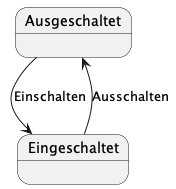
\includegraphics[width=0.25\textwidth]{fig/uml/lampe.png}
  \caption{Einfache FSM Lampe}
  \label{fig:lampe}
\end{figure}
Für die Erstellung einer geeigneten RESTful API mit HATEOAS (Hypermedia as the Engine of Application State) verwenden wir die folgende Struktur:
\\\\
Zustände abbilden:
\\
Ausgeschaltet: /lamp/off\\
Eingeschaltet: /lamp/on\\
\\\\
HTTP-Verben für Zustandsübergänge:
\\
Einschalten: PUT /lamp/on\\
Ausschalten: PUT /lamp/off
\\\\
Nun werden noch die HATEOAS-Links in den API-Antworten eingebunden. Somit ergibt sich ein Beispiel für eine JSON-Antwort, wenn die Lampe ausgeschaltet ist:\\\\
\noindent\begin{minipage}{\textwidth}
\begin{lstlisting}[caption={Fallbeispiel REST - aus},captionpos=b,label={lst:rest_on}]
{
  "state": "Ausgeschaltet",
  "links": [
    {
      "rel": "self",
      "href": "/lamp/off",
      "method": "GET"
    },
    {
      "rel": "Einschalten",
      "href": "/lamp/on",
      "method": "PUT"
    }
  ]
}
\end{lstlisting}
\end{minipage}

\noindent\begin{minipage}{\textwidth}
\begin{lstlisting}[caption={Fallbeispiel REST - an},captionpos=b,label={lst:rest_an}]
{
  "state": "Eingeschaltet",
  "links": [
    {
      "rel": "self",
      "href": "/lamp/on",
      "method": "GET"
    },
    {
      "rel": "Ausschalten",
      "href": "/lamp/off",
      "method": "PUT"
    }
  ]
}
\end{lstlisting}
\end{minipage}
Die JSON-Antworten enthalten den aktuellen Zustand der Lampe und HATEOAS-Links, die den möglichen Zustandsübergängen entsprechen. Dies ermöglicht es den Clients, die API dynamisch zu erkunden und zu verwenden, ohne die zugrunde liegende Struktur der API kennen zu müssen.\\\\

Liegt die Lösung der Software-Architektur als funktionale Zerlegung in der Grundarchitektur - beispielhaft - in einer MVC Architektur vor, könnte ein Adapter die Lücke zwischen der REST Architektur und der MVC Architektur schließen. Um einen Adapter zu erstellen, können wir das Adapter-Entwurfsmuster verwenden. Im Folgenden finden Sie ein Beispiel, das den vorherigen Ansatz modifiziert, um das MVC-Muster zu integrieren:


Um das Beispiel zu vereinfachen, wurde ein Python Syntax gewählt. Zuerst erstellen wir ein Lampenmodell, das die Logik für das Ein- und Ausschalten der Lampe enthält:\\\\
\noindent\begin{minipage}{\textwidth}
\begin{lstlisting}[caption={LampModel},captionpos=b,label={lst:lamp_m}]
class LampModel:
    def __init__(self):
        self.state = "AUS"

    def toggle(self):
        if self.state == "AUS":
            self.state = "EIN"
        else:
            self.state = "AUS"

    def get_state(self):
        return self.state

\end{lstlisting}
\end{minipage}
Dann erstellen wir einen Lampen-Controller, der das Modell verwendet und die Methoden on() und off() bereitstellt:\\\\
\noindent\begin{minipage}{\textwidth}
\begin{lstlisting}[caption={LampController},captionpos=b,label={lst:lamp_c}]
class LampController:
    def __init__(self, model):
        self.model = model

    def on(self):
        if self.model.get_state() == "AUS":
            self.model.toggle()

    def off(self):
        if self.model.get_state() == "EIN":
            self.model.toggle()
\end{lstlisting}
\end{minipage}
Schließlich erstellen wir einen Adapter, der den Lampen-Controller verwendet, um die Methoden on() und off() in der REST-API zu nutzen:\\\\
%\noindent\begin{minipage}{\textwidth}
\begin{lstlisting}[caption={LampAdapter},captionpos=b,label={lst:lamp_a}]
class LampAdapter(Resource):
    def __init__(self, controller):
        self.controller = controller

    def get(self):
        response = {
            "state": self.controller.model.get_state(),
            "_links": {
                "self": {"href": "/lamp"},
                "on": {"href": "/lamp/on"},
                "off": {"href": "/lamp/off"},
            }
        }
        return jsonify(response)

    def put(self):
        action = request.form.get("action")

        if action == "on":
            self.controller.on()
        elif action == "off":
            self.controller.off()

        response = {
            "state": self.controller.model.get_state(),
            "_links": {
                "self": {"href": "/lamp"},
                "on": {"href": "/lamp/on"},
                "off": {"href": "/lamp/off"},
            }
        }
        return jsonify(response)
\end{lstlisting}
%\end{minipage}
Zum Schluss integrieren wir den Adapter prototypisch in die Flask-App:\\\\
%\noindent\begin{minipage}{\textwidth}
\begin{lstlisting}[caption={Lamp REST APP},captionpos=b,label={lst:lamp_r}]
from flask import Flask, jsonify, request
from flask_restful import Resource, Api

app = Flask(__name__)
api = Api(app)

lamp_model = LampModel()
lamp_controller = LampController(lamp_model)
lamp_adapter = LampAdapter(lamp_controller)

api.add_resource(lamp_adapter, "/lamp", "/lamp/toggle", "/lamp/on", "/lamp/off")

if __name__ == "__main__":
    app.run(debug=True)
\end{lstlisting}
%\end{minipage}
Der Adapter verbindet nun das REST-Design mit dem MVC-Design. Die API unterstützt das Ein- und Ausschalten der Lampe über separate Endpunkte (/lamp/on und /lamp/off). Der Adapter verwendet den Lampen-Controller, um die on()- und off()-Methoden aufzurufen und auf das Modell zuzugreifen.
\\\\
Die vorgestellte Lösung ist ein Beispiel dafür, wie man das MVC-Design (Model-View-Controller) mit RESTful-APIs kombiniert, um sauberen und wartbaren Code zu schreiben. Es ist insofern üblich, als dass es bewährte Praktiken aus Software-Designmustern und Architekturen verwendet.

Es ist wichtig zu beachten, dass es keine \enquote{Einheitslösung} gibt, die auf alle Projekte oder Situationen anwendbar ist. Die beste Lösung hängt von den spezifischen Anforderungen und Bedingungen Ihres Projekts ab. In vielen Fällen ist es jedoch sinnvoll, Designmuster wie MVC und RESTful-APIs zu verwenden, um eine klare Trennung von Verantwortlichkeiten zu erreichen und die Komplexität des Codes zu reduzieren. Dies ist nur ein Beispiel, das die Anwendung dieser Prinzipien zeigt und kann als Ausgangspunkt für die Anpassung an die Anforderungen Ihres Projekts dienen. In der Praxis müssen Sie möglicherweise verschiedene Aspekte wie Skalierbarkeit, Performance und Sicherheit berücksichtigen und auf zusätzliche Anforderungen und Herausforderungen reagieren, die sich aus der realen Anwendung ergeben.
\\\\
Dennoch, die ReSTful-API eignet sich in dem Sinne der funktionalen Zerlegung für eine Lampe, da wir eine zeitliche Kopplung mit einem zustandslosen Dienst vorfinden. Sollten wir aber eine Echtzeitanforderung an die Schaltung der Lampe über Best-Effort formulieren, oder an der Lampe noch einen Bewegungsmelder mit automatischer Aktivierung der Lampe montieren, wirkt die Lösung mit der vorgestellten RESTful API nicht mehr attraktiv. 
\\\\
Diskutierbar ist auch ein weiteres Beispiel mit einer noch loseren zeitlichen Kopplung als über RESTful API Alternativen, oder der Nutzung leichtgewichtigerer Lösungen.
Alternativen zu RESTful API können zum Beispiel sein
\begin{itemize}
\item \textbf{CoAP} (Constrained Application Protocol): CoAP ist ein leichtgewichtiges, webbasiertes Protokoll, das speziell für eingeschränkte Umgebungen und Geräte entwickelt wurde. Es basiert auf dem REST-Architekturstil und verwendet das User Datagram Protocol (UDP) statt TCP, was es für den Einsatz in Low-Power- und verlustbehafteten Netzwerken geeignet macht. CoAP unterstützt die gleichen HTTP-Methoden wie GET, POST, PUT und DELETE und bietet eine einfache Möglichkeit, Ressourcen in IoT-Anwendungen zu identifizieren und zu manipulieren.
\item \textbf{XMPP} (Extensible Messaging and Presence Protocol): XMPP ist ein offenes, XML-basiertes Protokoll, das ursprünglich für Instant Messaging und Präsenzinformationen entwickelt wurde. Es ist ein erweiterbares und flexibles Protokoll, das auch für IoT-Anwendungen verwendet werden kann. XMPP bietet eine Vielzahl von Funktionen, wie beispielsweise die Fähigkeit, Nachrichten an mehrere Empfänger zu senden, und es unterstützt die Kommunikation über verschiedene Netzwerktopologien hinweg.
\item \textbf{AMQP} (Advanced Message Queuing Protocol): AMQP ist ein offenes, binäres Messaging-Protokoll, das für die Kommunikation zwischen Anwendungen und Systemen entwickelt wurde. Es ist ein zuverlässiges und sicheres Protokoll, das verschiedene Nachrichtenaustauschmuster wie Publish-Subscribe, Punkt-zu-Punkt und Request-Reply unterstützt. Im Vergleich zu MQTT ist AMQP komplexer und bietet mehr Funktionen, was es für den Einsatz in Enterprise-Anwendungen und für den Nachrichtenaustausch in verteilten Systemen geeignet macht.
\item \textbf{DDS} (Data Distribution Service): DDS ist ein Echtzeit-Publish-Subscribe-Protokoll, das für die Verteilung und den Austausch von Daten in Hochleistungs- und Echtzeitanwendungen entwickelt wurde. Es bietet Funktionen wie Quality of Service (QoS), Filterung und Sicherheit und eignet sich besonders für Anwendungen in Industrie, Verteidigung und Luft- und Raumfahrt.
\item \textbf{OPC-UA} (OPC Unified Architecture): OPC-UA ist ein industrielles Kommunikationsprotokoll, das für den Datenaustausch zwischen industriellen Steuerungssystemen und Automatisierungsgeräten entwickelt wurde. Es ist ein plattformunabhängiges, skalierbares und sicheres Protokoll, das eine Vielzahl von Funktionen bietet, wie z. B. Informationsmodellierung, Sicherheit und Discovery.
\end{itemize}
Die Auswahl des am besten geeigneten Protokolls hängt von den spezifischen Anforderungen und Zielen des Projekts ab. Dabei sollten Faktoren wie Bandbreite, Latenz, Sicherheit, Skalierbarkeit und Netzwerkumgebung berücksichtigt werden. Eine immer größere Beliebtheit haben Message Queue Broker Protokolle, die nun in einem eigenen Kapitel diskutiert werden.  

\subsubsection{IETF Message Broker Protokolle}

AMQP, STOMP und MQTT sind alle Protokolle, die für die Nachrichtenübertragung zwischen Systemen und Geräten aus dem Kontext der IETF verwendet werden können. Sie sind auf unterschiedliche Weise gestaltet und bieten unterschiedliche Funktionen, aber sie haben auch einige Gemeinsamkeiten. Alle drei Protokolle sind zustandsbasiert, was bedeutet, dass sie eine Verbindung zwischen dem Client und dem Broker herstellen und aufrechterhalten, um die Nachrichtenübertragung zu erleichtern. Sie verwenden alle einen Broker als Vermittler zwischen den Clients, um die Nachrichtenübertragung zu koordinieren und zu verwalten.
Alle drei Protokolle unterstützen eine Vielzahl von Anwendungen und können in verschiedenen Umgebungen wie IoT, Messaging-Systemen und anderen Anwendungsfällen eingesetzt werden.
Sie bieten alle eine hohe Skalierbarkeit, um die Anforderungen an die Nachrichtenübertragung in großen Systemen und Netzwerken zu erfüllen. 
\\\\
\textbf{AMQP}, die Abkürzung für Advanced Message Queuing Protocol, wurde als offener Ersatz für bestehende proprietäre Messaging-Middleware entwickelt. Zwei der wichtigsten Gründe für die Verwendung von AMQP sind Zuverlässigkeit und Interoperabilität. Wie der Name schon andeutet, bietet es eine breite Palette von Funktionen für das Messaging, einschließlich zuverlässiger Warteschlangen, themenbasiertem Publish-and-Subscribe-Messaging, flexiblem Routing, Transaktionen und Sicherheit. AMQP-Austausche leiten Nachrichten direkt weiter. Dies geschieht nach Themen (Topics) oder auch basierend auf Header-Informationen.

Bei einem so umfangreichen Funktionsumfang sind viele fein abgestufte Steuerungsmöglichkeiten vorhanden. Sie können den Zugriff auf Warteschlangen beschränken, ihre Tiefe verwalten und vieles mehr. Funktionen über Nachrichteneigenschaften, Anmerkungen und Header machen es zu einer guten Lösung für eine Vielzahl von Unternehmensanwendungen. Dieses Protokoll wurde für die Steigerung der Zuverlässigkeit vieler großer Unternehmensanwendungen entwickelt, die auf Messaging angewiesen sind, um Anwendungen zu integrieren und Daten innerhalb ihrer Organisation zu bewegen. AMQP ist ein binäres Protokoll, das für die Interoperabilität zwischen verschiedenen Anbietern entwickelt wurde. Wo andere Protokolle versagt haben, hat sich AMQP durchgesetzt. Unternehmen wie JP Morgan verwenden es zur Verarbeitung von 1 Milliarde Nachrichten pro Tag. Die NASA verwendet es für Nebula Cloud Computing. Google verwendet es für die komplexe Ereignisverarbeitung. Es wird in einer der weltweit größten biometrischen Datenbanken verwendet, dem indischen Aadhar-Projekt, das 1,2 Milliarden Identitäten enthält. Es wird in der Ocean Observatories Initiative verwendet - eine Architektur, die täglich 8 Terabyte an Daten sammelt. 
\\\\
\textbf{MQTT} (Message Queue Telemetry Transport) wurde ursprünglich vom IBM-Team für Pervasive Computing und dessen Arbeit mit Partnern aus der Industrie entwickelt. In den letzten Jahren wurde das Protokoll in die Open-Source-Gemeinschaft überführt, erfuhr mit dem Aufschwung mobiler Anwendungen einen beträchtlichen Popularitätszuwachs. Die Konstruktionsprinzipien und Ziele von MQTT sind viel einfacher und zielgerichteter als die von AMQP - es bietet Publish-and-Subscribe-Messaging (keine Warteschlangen, trotz des Namens) und wurde speziell für ressourcenbeschränkte Geräte und Netzwerke mit geringer Bandbreite und hoher Latenz entwickelt. Im Grunde kann es besonders in eingebetteten Systemen effektiv eingesetzt werden.

Einer der Vorteile von MQTT gegenüber vollwertigen \enquote{Enterprise Messaging}-Brokern besteht darin, dass es aufgrund seines absichtlich geringen Platzbedarfs ideal für die heutigen mobilen und sich entwickelnden Anwendungen im Stil des \enquote{Internet der Dinge} ist. Unternehmen wie Facebook verwenden es sogar als Teil ihrer mobilen Anwendungen, weil es so wenig Strom verbraucht und die Netzwerkbandbreite schont.

Einige der MQTT-basierten Broker unterstützen viele tausend gleichzeitige Geräteverbindungen. MQTT bietet drei Dienstqualitäten.

Die Stärken von MQTT sind Einfachheit (nur fünf API-Methoden), eine kompakte binäre Paket-Nutzlast (keine Nachrichteneigenschaften, komprimierte Header, viel weniger ausführlich als etwas Textbasiertes wie HTTP), und es eignet sich gut für einfache Push-Nachrichten-Szenarien wie Temperatur-Updates, Börsenticker, Öldruck-Feeds oder mobile Benachrichtigungen. Es ist auch sehr nützlich, um Maschinen miteinander zu verbinden, z. B. um ein Arduino-Gerät mit einem Webdienst über MQTT zu verbinden.
\\\\
\textbf{STOMP} (Simple/Streaming Text Oriented Messaging Protocol) ist das einzige dieser drei Protokolle, das textbasiert ist und damit in Bezug auf sein Erscheinungsbild eher mit HTTP vergleichbar ist. Wie AMQP bietet STOMP einen Nachrichten- (oder Rahmen-) Header mit Eigenschaften und einen Rahmenkörper. Die Entwurfsprinzipien waren hier, etwas Einfaches und weitgehend Interoperables zu schaffen. So ist es beispielsweise möglich, eine Verbindung zu einem STOMP-Broker mit einem einfachen Telnet-Client herzustellen.

STOMP arbeitet jedoch nicht mit Warteschlangen und Themen, sondern verwendet eine SEND-Semantik mit einer \enquote{Ziel}-String. Der Broker muss auf etwas abbilden, das er intern versteht, wie z. B. ein Thema, eine Warteschlange oder einen Austausch. Die Verbraucher SUBSCRIBEN dann zu diesen Zielen. Da diese Ziele in der Spezifikation nicht vorgeschrieben sind, können verschiedene Broker unterschiedliche Arten von Zielen unterstützen. Daher ist es nicht immer einfach, Code zwischen Brokern zu portieren.

STOMP ist jedoch einfach und leichtgewichtig (wenn auch etwas langatmig auf dem Draht), mit einer breiten Palette von Sprachbindungen. Es bietet auch einige transaktionale Semantiken. Eines der interessantesten Beispiele ist RabbitMQ Web Stomp, mit dem Sie Nachrichten in einem Browser über Websockets bereitstellen können. Dies eröffnet einige interessante Möglichkeiten, z. B. die Aktualisierung eines Browsers, einer mobilen Anwendung oder einer Maschine in Echtzeit mit allen Arten von Informationen.

\subsubsection{Message Broker}
Das Skript legt im weiteren weniger Wert auf STOMP oder AMQP, sondern legt zunächst den Fokus auf MQTT und vergleicht es gegenüber einem proprietären Protokoll aus dem APACHE Kafka Kontext. MQTT steht für ein Beipiel bei der Unterstützung einer Vielzahl von Geräten und Apache Kafka für die Etablierung einer hohen Verarbeitung von einer Vielzahl von Transaktionen.
\\\\
MQTT (Message Queuing Telemetry Transport) und Apache Kafka sind zwei verschiedene Protokolle bzw. Systeme, die für die Kommunikation in verteilter Umgebung und für die Verarbeitung von Datenströmen entwickelt wurden. Sie haben unterschiedliche Anwendungsfälle und Eigenschaften. Hier ist eine Diskussion über die Hauptunterschiede zwischen MQTT und Kafka:
\\\\
MQTT ist wie erwähnt ein leichtgewichtiges Publish-Subscribe-Protokoll, das speziell für eingeschränkte Umgebungen und Geräte mit begrenzter Rechenleistung und Bandbreite entwickelt wurde. Apache Kafka hingegen ist ein verteiltes Streaming-System, das für die Verarbeitung großer Datenmengen und Hochdurchsatz-Workloads entwickelt wurde. Es ist ein skalierbares und fehlertolerantes System, das für die Kommunikation zwischen großen verteilten Anwendungen und für die Verarbeitung und Speicherung von Datenströmen in Echtzeit verwendet wird.
\\\\
Während MQTT für Szenarien entwickelt wurde, in denen eine geringe Latenz und geringer Bandbreitenverbrauch wichtig sind, ist Kafka für den Datenaustausch und die Verarbeitung in groß angelegten, verteilten Anwendungen und Systemen entwickelt worden.

MQTT bietet eine Quality of Service (QoS) für die Nachrichtenübertragung, die es ermöglicht, unterschiedliche Grade der Zuverlässigkeit und Garantien für die Nachrichtenübermittlung zu wählen. Auf der anderen Seite bietet Kafka starke Haltbarkeits- und Verarbeitungsgarantien, indem es eine replizierte, verteilte und fehlertolerante Architektur verwendet.
\paragraph{MQ Technologiestacks\\\\}
Auch Kafka, wenngleich sehr stark verbreitet ist in seinem Kontext - wie MQTT in seinem - ist nicht ohne Alternativen. Es gibt verschiedene alternative Technologien zu Apache Kafka, die für ähnliche Anwendungszwecke wie das Verarbeiten von Datenströmen und die Kommunikation in verteilten Systemen verwendet werden können. Einige der bekanntesten sind:
\begin{itemize}
\item Apache Pulsar: Apache Pulsar ist ein verteiltes Messaging-System und Event-Streaming-Plattform, die für hohe Skalierbarkeit, Durchsatz und niedrige Latenz entwickelt wurde. Pulsar bietet eine getrennte Architektur für Messaging und Speicherung, was es ermöglicht, den Durchsatz und die Speicherkapazität unabhängig voneinander zu skalieren. Pulsar unterstützt auch Funktionen wie Geo-Replikation und Multi-Tenancy und kann als Alternative zu Kafka für Anwendungsfälle in verteilten Systemen und Echtzeit-Datenverarbeitung verwendet werden.
\item NATS Streaming: NATS Streaming ist ein leichtgewichtiges, hochleistungsfähiges Messaging-System, das auf dem NATS-Core-Protokoll aufbaut und zusätzliche Funktionen für die Verarbeitung von Datenströmen bereitstellt. Es bietet Funktionen wie At-least-once-Delivery, Nachrichten-Acknowledgements und Nachrichten-Historie. NATS Streaming ist für seine Einfachheit und geringe Latenz bekannt und kann für Anwendungsfälle verwendet werden, in denen schnelle Nachrichtenübermittlung und Echtzeit-Verarbeitung erforderlich sind.
\item Amazon Kinesis: Amazon Kinesis ist ein vollständig verwalteter Streaming-Datendienst, der von AWS bereitgestellt wird. Kinesis ermöglicht das Sammeln, Verarbeiten und Analysieren von Echtzeit-Datenströmen und bietet Funktionen wie skalierbare Dateneingabe und automatische Skalierung. Kinesis ist gut in das AWS-Ökosystem integriert und kann für Anwendungsfälle verwendet werden, in denen Echtzeit-Datenverarbeitung, -analyse und -überwachung erforderlich sind.
\item Google Cloud Pub/Sub: Google Cloud Pub/Sub ist ein Messaging- und Event-Streaming-Dienst, der von Google Cloud bereitgestellt wird. Pub/Sub ermöglicht die asynchrone Kommunikation zwischen verteilten Systemen und unterstützt Publish-Subscribe- und Point-to-Point-Messaging-Muster. Es ist gut in das Google Cloud-Ökosystem integriert und bietet Funktionen wie At-least-once-Delivery und automatische Skalierung.
\end{itemize}

Tatsächlich sind in dieser Aufzählung Technologien und Protokolle vermischt, die für Messaging und Datenverarbeitung verwendet werden. Der Grund dafür ist, dass in vielen Anwendungsfällen wie verteilten Systemen und Echtzeit-Datenverarbeitung, die Technologien und Protokolle eng miteinander verknüpft sind und oft zusammen verwendet werden, um bestimmte Funktionen zu erreichen und somit kaum mehr zwischen dem Protokoll und der technologischen Umsetzung unterschieden wird. Dies trifft nicht zuletzt sogar für Kafka zu. 

Apache Kafka ist sowohl ein Protokoll als auch eine Technologie, die auf dem Protokoll basiert. Es ist ein Messaging- und Streaming-System, das auf seinem eigenen Protokoll aufbaut. Somit wurde - zum besseren Verständnis - in der Aufzählung nur versucht, alternative Technologien und Protokolle zu nennen, die auch ähnliche Anwendungsfälle wie Kafka abdecken können. Es ist jedoch wichtig, zwischen den Protokollen und den Technologien, die diese Protokolle implementieren, zu unterscheiden. Dies ist aber besser am Beispiel MQTT diskutiert.
\\\\
Gerade die Vielzahl der Umsetzung von Message Broker mit MQTT Unterstützung können selbst den geneigtesten Leser irritiert zurück lassen\footnote{\url{https://github.com/hobbyquaker/awesome-mqtt}}. Aus diesem sehr großen Kontext, können beispielhaft RabbitMQ und ZeroMQ genannt werden. RabbitMQ, ZeroMQ und andere Messaging-Lösungen bieten unterschiedliche Funktionen und Eigenschaften, die sie für verschiedene Anwendungsfälle und Umgebungen geeignet machen. Die Vielzahl von Message-Broker-Implementierungen existiert, weil es eine breite Palette von Anforderungen und Szenarien in verteilten Systemen und Echtzeit-Kommunikation gibt, die von verschiedenen Lösungen besser oder schlechter abgedeckt werden können.
\\\\
RabbitMQ ist ein Open-Source-Message-Broker, der neben dem MQTT auch das Advanced Message Queuing Protocol (AMQP) implementiert. Es unterstützt verschiedene Messaging-Szenarien wie Publish-Subscribe, Point-to-Point und Request-Reply. RabbitMQ ist für seine Robustheit, Zuverlässigkeit und Skalierbarkeit bekannt und eignet sich für Enterprise-Anwendungen und für den Einsatz in verteilten Systemen.
\\\\
ZeroMQ hingegen ist eine leichtgewichtige Messaging-Bibliothek, die für hohe Leistung und geringe Latenz optimiert ist. Im Gegensatz zu RabbitMQ, das als zentralisierter Broker fungiert, ist ZeroMQ brokerlos und ermöglicht den direkten Austausch von Nachrichten zwischen Anwendungen oder Prozessen. ZeroMQ bietet verschiedene Kommunikationsmuster wie Publish-Subscribe, Request-Reply und Pipeline. Es eignet sich für Anwendungsfälle, in denen schnelle Kommunikation, geringe Latenz und einfache Skalierbarkeit erforderlich sind.
\\\\
Wichtig ist aber zu verstehen, das bei der Vielzahl der Angebote die Grundarchitektur immer sehr ähnlich ist, das folgende Kapitel wird es exemplarisch diskutieren.

\subsubsection{Message Broker Architektur}

Die Wahl der richtigen Messaging-Lösung hängt von Faktoren wie Skalierbarkeit, Latenz, Zuverlässigkeit, Kommunikationsmuster und Integration in bestehende Infrastrukturen ab. Die Vielzahl von Message-Broker-Implementierungen ermöglicht es Entwicklern, die beste Lösung für ihre Anwendungsfälle auszuwählen, indem sie die spezifischen Anforderungen ihrer Projekte und die Eigenschaften der verfügbaren Messaging-Lösungen berücksichtigen. Durch das Verständnis der Unterschiede zwischen diesen Lösungen können Entwickler fundierte Entscheidungen über die Auswahl der richtigen Messaging-Technologie für ihre Projekte treffen. Das Bauchgefühl ist hier keine gute Entscheidungsgrundlage. 
\\\\
In dem bisherigen Text sind aus Sicht des Autors die neun wichtigsten - aufgrund ihrer Marktverbreitung und Popularität - Message Broker genannt worden, zur Vervollständigung einer - wenngleich nicht die - Top 10 kann noch die IBM MQ (früher WebSphere MQ) genannt werden. Ein proprietärer Message-Broker von IBM, der für seine Zuverlässigkeit, Sicherheit und Integration in IBM-Systeme und andere Enterprise-Anwendungen bekannt ist.
\\\\
Bei IBM MQ handelt es sich um einen Middleware-Service, der eine asynchrone und zuverlässige Nachrichtenübermittlung zwischen den Systemen gewährleistet und diese Eigenschaft mit den meisten der hier genannten Systemen teilt. Hier lohnt sich in der Diskussion insbesondere ein Blick auf die internen Komponenten, dass diese nicht selten und dabei nicht zu Letzt von \cite{tanenbaum2017distributed} als Referenz herangezogen werden.
\\\\
Die innere Architektur von IBM MQ besteht aus mehreren Komponenten, die zusammenarbeiten, um eine zuverlässige und sichere Nachrichtenübermittlung zu gewährleisten:

\begin{itemize}
\item Message Queues: IBM MQ verwendet Warteschlangen, um Nachrichten zwischen den Systemen zu übermitteln. Die Anwendungen senden und empfangen Nachrichten über diese Warteschlangen, die als Puffer für Nachrichten dienen. Dadurch können Anwendungen unabhängig voneinander arbeiten und Systemausfälle abfedern, ohne dass Nachrichten verloren gehen.
\item Message Channel Agents (MCAs): MCAs sind verantwortlich für die Übertragung von Nachrichten zwischen den MQ-Servern (auch als Queue-Managern bezeichnet). Sie sorgen dafür, dass die Nachrichten sicher und zuverlässig zwischen den Systemen übertragen werden, indem sie Funktionen wie Verschlüsselung, Komprimierung und Nachrichten-Acknowledgements bereitstellen.
\item Queue Manager: Der Queue Manager ist das Herzstück von IBM MQ und verwaltet die Warteschlangen und die Nachrichtenübermittlung. Er ist dafür verantwortlich, die Nachrichten zwischen den Warteschlangen zu übertragen, die Nachrichtenpersistenz sicherzustellen und die Verarbeitung von Nachrichten zu steuern.
\item Clients: IBM MQ Clients sind Anwendungen, die auf Client-Systemen ausgeführt werden und mit dem IBM MQ Server über das Message Queue Interface (MQI) kommunizieren. Die Clients senden und empfangen Nachrichten über die Warteschlangen und können in verschiedenen Programmiersprachen geschrieben sein.
\end{itemize}

Unter der Haube wird das Publish-Subscribe-Pattern in der Regel durch eine Message Queue implementiert. Der Publisher sendet die Nachrichten an eine Queue, die für die Empfänger zugänglich ist. Die Empfänger können sich auf die Queue abonnieren, um die Nachrichten zu erhalten, die vom Publisher gesendet werden. Sobald eine neue Nachricht in der Queue eintrifft, wird sie an alle Abonnenten der Queue verteilt.
\\\\
Das Pub-Sub-Muster kann auch durch andere Mechanismen implementiert werden, wie z.B. durch die Verwendung von Topics oder Channels. In diesem Fall sendet der Publisher die Nachrichten an einen bestimmten Topic oder Channel, und die Empfänger abonnieren den entsprechenden Topic oder Channel, um die Nachrichten zu erhalten.
\\\\
Es gibt verschiedene Möglichkeiten, die Priorisierung von Nachrichten in einer Publish-Subscribe-Architektur umzusetzen.

Eine Möglichkeit ist die Verwendung von Prioritätsniveaus, bei der jede Nachricht eine Priorität zugewiesen wird. Die Prioritäten können je nach der Bedeutung der Nachricht oder dem Zeitrahmen, innerhalb dessen sie verarbeitet werden muss, variiert werden. Die Message Queue kann dann so konfiguriert werden, dass sie die höher priorisierten Nachrichten zuerst verarbeitet.

Eine weitere Möglichkeit ist die Verwendung von Routing-Regeln, bei der die Nachrichten basierend auf bestimmten Kriterien an bestimmte Empfänger weitergeleitet werden. Diese Kriterien können beispielsweise der Inhalt der Nachricht, der Sender oder der Empfänger sein. Durch die Verwendung von Routing-Regeln können Nachrichten an die richtigen Empfänger weitergeleitet werden, basierend auf ihrer Priorität.

Es gibt auch spezialisierte Software-Tools, die die Priorisierung von Nachrichten in Publish-Subscribe-Systemen unterstützen. Zum Beispiel kann Apache Kafka Konfigurationen bereitstellen, um die Reihenfolge der Verarbeitung von Nachrichten zu steuern und das Verarbeiten von höher priorisierten Nachrichten zu priorisieren.

\subsubsection{Fehlersemantik}

Neben der Priorisierung ist auch die Qualität der Dienstleistung (QoS) entscheidend für den Erfolg, insbesondere die damit verbundenen Fehlersemantik. Dies soll am Beispiel von MQTT diskutiert werden.
MQTT unterstützt drei QoS-Levels (0, 1 und 2), die unterschiedliche Garantien bezüglich der Nachrichtenzustellung bieten, die im Folgenden  auch allgemeine diskutiert werden sollen. 
\begin{itemize}
\item QoS 0 - Maybe: QoS 0 bedeutet, dass Nachrichten nach Best Effort QoS zugestellt werden. Es gibt keine Garantie für die Zustellung, und es ist möglich, dass Nachrichten verloren gehen oder dupliziert werden. Dieses Level ist ideal für Anwendungsfälle, bei denen Datenverlust oder Duplikate tolerierbar sind, z. B. bei Sensordaten, die kontinuierlich übertragen werden. Die Fehlersemantik in diesem Level ist \enquote{maybe} (vielleicht), da die Zustellung nicht garantiert ist.
\item QoS 1 - At-least-once (Mindestens einmal):
Bei QoS 1 wird sichergestellt, dass Nachrichten mindestens einmal zugestellt werden. Dies bedeutet, dass der Sender die Nachricht wiederholt sendet, bis eine Empfangsbestätigung (ACK) vom Empfänger erhalten wird. Dieses Level ist ideal für Anwendungsfälle, bei denen die Zustellung wichtiger ist, und Datenverlust vermieden werden muss. Die Fehlersemantik in diesem Level ist \enquote{at-least-once"}(mindestens einmal), da Nachrichten möglicherweise mehrmals zugestellt werden.
\item QoS 2 - Exactly-once (Genau einmal):
QoS 2 garantiert, dass Nachrichten genau einmal zugestellt werden. Dieses Level stellt sicher, dass keine Nachrichten verloren gehen oder dupliziert werden. Um dies zu erreichen, wird ein Vier-Wege-Handshake-Verfahren zwischen Sender und Empfänger durchgeführt, das den Nachrichtenaustausch koordiniert. Dieses Level ist ideal für Anwendungsfälle, bei denen sowohl Datenverlust als auch Duplikate unzulässig sind, z. B. bei Steuerungs- oder Transaktionsdaten. Die Fehlersemantik in diesem Level ist \enquote{exactly-once} (genau einmal), da Nachrichten garantiert nur einmal zugestellt werden.
\end{itemize}

Die Fehlersemantiken at-least-once, at-most-once und exactly-once beziehen sich auf die Garantien, die ein Kommunikationssystem oder ein Protokoll hinsichtlich der Zustellung von Nachrichten bietet und können noch allgemein gesprochen um maybe erweitert werden. Sie haben einen signifikanten Einfluss auf die Architektur und das Verhalten von Systemen in Bezug auf Stateless- oder Stateful-Charakteristiken, Geschwindigkeit und Blockierungen:
\begin{itemize}
\item  Maybe (Vielleicht): Die maybe-Fehlersemantik bedeutet, dass die Nachrichtenzustellung nicht garantiert ist und Nachrichten möglicherweise verloren gehen können. Systeme, die diese Semantik verwenden, sind in der Regel stateless, da sie keine Informationen über den Zustand der Nachrichtenübermittlung speichern. Die Geschwindigkeit ist in der Regel hoch, da es keine zusätzlichen Schritte oder Wiederholungen zur Sicherstellung der Zustellung gibt. Da keine Blockierungen aufgrund von Zustellungsbestätigungen oder wiederholten Nachrichtenübermittlungen auftreten, ist die Kommunikation in solchen Systemen meist reibungslos.
\item At-most-once (Höchstens einmal): Die at-most-once-Fehlersemantik stellt sicher, dass Nachrichten höchstens einmal zugestellt werden. Ähnlich wie bei der maybe-Semantik sind Systeme, die diese Semantik verwenden, in der Regel stateless und schneller, da sie keine zusätzlichen Schritte zur Überprüfung der Nachrichtenzustellung durchführen. Diese Systeme können jedoch Nachrichten verlieren, sind aber vor Duplikaten geschützt. Blockierungen sind minimal, da keine Zustellungsbestätigungen erwartet werden.
\item At-least-once (Mindestens einmal): Die at-least-once-Fehlersemantik garantiert, dass Nachrichten mindestens einmal zugestellt werden. Systeme, die diese Semantik verwenden, sind in der Regel stateful, da sie den Zustand von Nachrichtenübermittlungen und Bestätigungen speichern müssen. Die Geschwindigkeit dieser Systeme kann aufgrund der zusätzlichen Schritte, wie dem Warten auf Empfangsbestätigungen (ACKs) und möglichen Wiederholungen, beeinträchtigt werden. Blockierungen können auftreten, wenn ein System auf Zustellungsbestätigungen wartet oder wiederholte Nachrichtenübermittlungen durchführt.
\item Exactly-once (Genau einmal): Die exactly-once-Fehlersemantik garantiert, dass Nachrichten genau einmal zugestellt werden. Systeme, die diese Semantik verwenden, sind stateful, da sie den Zustand von Nachrichtenübermittlungen, Bestätigungen und zusätzlichen Handshakes verwalten müssen. Die Geschwindigkeit dieser Systeme ist im Vergleich zu den anderen Semantiken am niedrigsten, da mehr Schritte und Kommunikationsaustausch erforderlich sind, um die exakte Zustellung zu gewährleisten. Blockierungen sind häufiger, da Systeme auf Handshakes und Bestätigungen warten, um den Nachrichtenübermittlungsprozess abzuschließen.
\end{itemize}
In verteilten Systemen ist die Exactly-Once-Fehlersemantik (auch bekannt als \enquote{Exactly Once Delivery} oder \enquote{Exactly Once Processing}) ein wichtiges Konzept, bei dem eine Nachricht genau einmal erfolgreich verarbeitet wird. Die Idee ist, dass Daten weder verloren gehen noch doppelt verarbeitet werden. In der Praxis ist die Exactly-Once-Fehlersemantik im eigentlichen Sinne jedoch unmöglich, da verteilte Systeme immer von Unsicherheiten und Unvorhersehbarkeiten betroffen sind.

Einige der Hauptgründe, warum die Exactly-Once-Fehlersemantik im eigentlichen Sinne unmöglich ist, sind:
\begin{itemize}
\item Zwei-Generäle-Problem: Das ist ein bekanntes Problem in der Informatik, das zeigt, dass es in verteilten Systemen keine Garantie dafür geben kann, dass zwei Parteien zuverlässig zu einer Übereinkunft kommen, wenn es Unsicherheiten bei der Kommunikation gibt (z.B. Nachrichtenverlust). Dies wird im folgenden Text auch nochmals intensiver diskutiert.
\item Unzuverlässige Kommunikation: Netzwerke können unzuverlässig sein, und es ist möglich, dass Nachrichten verloren gehen, beschädigt oder verzögert werden. Dies erschwert die Implementierung einer Exactly-Once-Fehlersemantik.
\item Unvorhersehbare Systemausfälle: Verteilte Systeme sind anfällig für Hardware- oder Softwareausfälle. Es ist schwierig, eine Exactly-Once-Fehlersemantik zu gewährleisten, wenn man nicht genau wissen kann, welche Komponenten ausfallen und wann dies geschehen könnte.
\end{itemize}
Trotz dieser Herausforderungen gibt es Protokolle wie MQTT (Message Queuing Telemetry Transport), die eine Exactly-Once-Fehlersemantik versprechen. Dies wird durch die Implementierung eines Mechanismus zur Kontrolle der Nachrichtenübermittlung erreicht. Es ist wichtig zu betonen, dass MQTT eine Annäherung an die Exactly-Once-Fehlersemantik bietet und in den Definitionen unterschieden wird zwischen  \textbf{message delivery} und \enquote{message processing}.\footnote{\url{https://exactly-once.github.io/posts/exactly-once-delivery/}}

\paragraph{Zwei-Generäle-Problem \\\\}
Das grundsätzliche Problem kann mit den Zwei-Generäle-Problem argumentiert werden. Das Two Generals' Problem, auch bekannt als das Byzantinische Generäle Problem, ist ein klassisches Problem in der Informatik und Kommunikationstheorie, dass sich mit der Frage der Koordination und Vertrauensbildung zwischen zwei Parteien befasst, die über einen unzuverlässigen Kommunikationskanal kommunizieren.
\\\\
Stellen Sie sich vor, es gibt zwei Generäle, General A und General B, die jeweils eine Armee kommandieren. Sie planen, eine feindliche Stadt anzugreifen und müssen sich auf den genauen Zeitpunkt des Angriffs einigen. Sie sind jedoch räumlich getrennt und können nur über Boten kommunizieren, die Nachrichten zwischen ihnen hin- und hertragen. Das Problem ist, dass der Kommunikationsweg durch das feindliche Gebiet führt und es eine Chance gibt, dass Boten abgefangen und ihre Nachrichten verloren gehen.

Um den Angriff erfolgreich durchzuführen, müssen sich beide Generäle auf den gleichen Zeitpunkt einigen und sicher sein, dass der andere General die Nachricht empfangen hat und mit dem Plan einverstanden ist. Wenn einer der Generäle angreift, während der andere sich zurückhält, wird der Angriff fehlschlagen und beide Armeen werden vermutlich besiegt werden.

Nehmen wir an, General A entscheidet sich für einen Angriffszeitpunkt und sendet einen Boten zu General B, um ihn über den Plan zu informieren. Es gibt jedoch keine Garantie, dass der Bote General B erreicht. Selbst wenn der Bote General B erreicht, wie kann General A sicher sein, dass die Nachricht erfolgreich zugestellt wurde?

Um dies zu bestätigen, könnte General B einen Boten zurückschicken, um zu bestätigen, dass er die Nachricht erhalten hat und mit dem Angriffszeitpunkt einverstanden ist. Aber was, wenn dieser bestätigende Bote verloren geht? Dann wird General A nicht wissen, ob General B die ursprüngliche Nachricht erhalten hat, und der Angriff wird gefährdet sein.

Das Two Generals' Problem zeigt, dass es in solchen Szenarien unmöglich ist, eine absolute Gewissheit der Koordination und Übereinstimmung zwischen den beiden Parteien zu erreichen, wenn der Kommunikationskanal unzuverlässig ist. Dieses Problem ist relevant für die Informatik, insbesondere in verteilten Systemen und Netzwerken, bei denen Kommunikationskanäle nicht immer zuverlässig sind und Knoten möglicherweise nicht vertrauenswürdig sind.
\\\\
In der Praxis verwenden verteilte Systeme und Netzwerke verschiedene Techniken, um den Grad der Koordination und Konsistenz zu erhöhen, wie z. B. Konsensalgorithmen (z. B. Paxos oder Raft) oder fehlertolerante Protokolle. Diese Protokolle werden noch in einem späteren Kapitel genauer diskutiert. wie es auch sei, diese Lösungen bieten jedoch auch keine absolute Garantie, sondern erhöhen lediglich die Wahrscheinlichkeit einer erfolgreichen Kommunikation und Koordination.

\paragraph{Exactly-Once-Fehlersemantik mit MQTT\\\\}

Es ist schwierig, eine exakte Wahrscheinlichkeitsberechnung für das Auftreten eines Fehlers bei der Exactly-Once-Fehlersemantik mit MQTT QoS 2 anzugeben, da dies von vielen Faktoren abhängt, wie zum Beispiel der Zuverlässigkeit des Netzwerks, der verwendeten Hardware und Software, sowie von Umweltbedingungen. Stattdessen können wir eine grobe Schätzung der Wahrscheinlichkeit solcher Fehler basierend auf einigen Annahmen diskutieren.

Angenommen, die Wahrscheinlichkeit, dass eine einzelne Nachricht während der Übertragung verloren geht, ist p (z.B. p = 0.001 oder 0.1 \%). Diese Wahrscheinlichkeit kann aufgrund von Netzwerkproblemen, Hardware- oder Softwareausfällen auftreten.

In einem QoS 2-Szenario gibt es vier Hauptnachrichten, die zwischen Sender und Empfänger (bzw. Broker) ausgetauscht werden: PUBLISH, PUBREC, PUBREL und PUBCOMP. Für den Exactly-Once-Fehlersemantik-Fehler muss eine dieser Nachrichten verloren gehen, während gleichzeitig der Wiederholungsmechanismus von MQTT versagt.

Die Wahrscheinlichkeit, dass eine dieser vier Nachrichten verloren geht, kann mit der Formel $1 - (1 - p)^4$ berechnet werden, da wir annehmen, dass die Wahrscheinlichkeiten unabhängig voneinander sind.
\\\\
Für p = 0,001 (0,1 \%) erhalten wir:
\\\\
$1 - (1 - 0.001)^4 \approx 0.00397$ oder $0.397 \%$
\\\\
Die Wahrscheinlichkeit, dass eine der vier Hauptnachrichten verloren geht, beträgt also etwa 0.397 \%. Dies ist jedoch noch nicht die endgültige Wahrscheinlichkeit für das Versagen der Exactly-Once-Fehlersemantik, da wir auch den Wiederholungsmechanismus von MQTT berücksichtigen müssen.

Angenommen, der Wiederholungsmechanismus funktioniert mit einer Zuverlässigkeit von q (z.B. q = 0.999 oder 99.9 \%). Die Wahrscheinlichkeit, dass der Wiederholungsmechanismus ebenfalls versagt, beträgt (1 - q).

Die kombinierte Wahrscheinlichkeit für das Versagen der Exactly-Once-Fehlersemantik ist dann die Wahrscheinlichkeit, dass eine der vier Nachrichten verloren geht, multipliziert mit der Wahrscheinlichkeit, dass der Wiederholungsmechanismus versagt:
\\\\
$0.00397 * (1 - 0.999) \approx 0.00000397 oder 0.000397 \%$
\\\\
In diesem Beispiel beträgt die Wahrscheinlichkeit, dass die Exactly-Once-Fehlersemantik versagt, etwa 0.000397 \%, wenn wir die oben genannten Annahmen treffen. Es ist wichtig zu betonen, dass diese Berechnung stark von den angenommenen Wahrscheinlichkeiten p und q abhängt und in der Praxis variieren kann.

Trotzdem zeigt das Beispiel, dass die Wahrscheinlichkeit eines Versagens der Exactly-Once-Fehlersemantik in einem gut konfigurierten MQTT-System mit QoS 2 sehr gering ist, solange die Netzwerk-, Hardware- und Softwarebedingungen zuverlässig sind.

Und somit ist es erwähnenswert, dass trotz solcher Ausnahmefälle MQTT mit QoS 2 eine hohe Zuverlässigkeit bei der Nachrichtenübermittlung bietet, indem es den Nachrichtenaustausch koordiniert und den Zustand der Nachrichten beibehält. Solche Szenarien sind extrem selten, und MQTT ist in der Regel in der Lage, die Exactly-Once-Fehlersemantik erfolgreich durchzuführen. Dennoch eine 100 \%-ige Sicherheit ist es nicht, dies wird uns auch nochmal zu einem späteren Zeitpunkt begleiten. 

\paragraph{Message Broker in der Praxis\\\\}

Bei Message Brokern werden oft einige Aspekte unterschätzt, die zu Herausforderungen führen können. Hier sind einige Beispiele:

\begin{itemize}
\item Komplexität: Die Einrichtung und Konfiguration eines Message Brokers kann sehr komplex sein. Es erfordert ein tiefes Verständnis der Funktionsweise des Brokers sowie der Anforderungen der Anwendung, die ihn nutzt.
\item Ausfallsicherheit: Da Message Broker oft eine zentrale Rolle in der Architektur einnehmen, müssen sie in der Regel sehr ausfallsicher sein. Ein Ausfall des Brokers kann schwerwiegende Folgen für die gesamte Anwendung haben.
\item Skalierbarkeit: Skalierbarkeit ist ein wichtiger Aspekt von Message Brokern. Wenn die Anzahl der Nachrichten oder der Verkehr auf der Plattform zunimmt, muss der Broker in der Lage sein, diese Last zu bewältigen.
\item Leistung: Die Leistung von Message Brokern ist ein weiterer wichtiger Aspekt, der oft unterschätzt wird. Wenn die Verarbeitungsgeschwindigkeit von Nachrichten nicht ausreicht, kann dies zu Verzögerungen in der Anwendung führen.
\item Sicherheit: Message Broker müssen sicher sein, um sicherzustellen, dass vertrauliche oder sensible Informationen nicht in die falschen Hände geraten.
\item Kompatibilität: Da Message Broker in der Regel in verschiedenen Anwendungen und Systemen eingesetzt werden, muss die Kompatibilität mit anderen Systemen sichergestellt werden, um eine reibungslose Integration zu ermöglichen.
\item Wartung und Support: Die Wartung und Unterstützung von Message Brokern kann sehr zeitaufwändig sein. Es ist wichtig, sicherzustellen, dass der Broker regelmäßig gewartet und aktualisiert wird, um sicherzustellen, dass er sicher und zuverlässig bleibt.
\end{itemize}
Das führt wiederum zu neuen Geschäftsmodellen, wo die Nutzung des Message Brokers im Grunde verschenkt wird, um den Nutzer an die Service Leistungen zu binden, die im besten Fall die Nachteile des Systems auffangen. 
Ein Beispiel ist hier HiveMQ. HiveMQ ist ein kommerzielles MQTT-Messaging-System, das auf die Implementierung von IoT-Plattformen und -Anwendungen spezialisiert ist. Das Unternehmen bietet sowohl eine Cloud-basierte als auch eine On-Premises-Version seines Produkts an und generiert Einnahmen durch den Verkauf von Lizenzen und den Abschluss von Abonnements.
\\\\
Das Hauptgeschäftsmodell von HiveMQ basiert auf der Lizenzierung seiner Messaging-Plattform an Unternehmen, die diese für ihre IoT-Anwendungen nutzen möchten. Es gibt verschiedene Lizenzierungsmodelle, die je nach den Anforderungen des Kunden angepasst werden können. Dazu gehören beispielsweise Abonnements auf Jahresbasis, die je nach der Anzahl der verbundenen Geräte oder der Anzahl der Nachrichten, die über die Plattform übertragen werden, gestaffelt sind.

HiveMQ bietet auch eine kostenlose Community-Version seiner Plattform an, die jedoch weniger Funktionen und Support bietet als die kommerzielle Version. 

Wichtig für den Erfolg eines Protokolls ist wie bereits öfter angesprochen das API Design. Am Ende entscheiden die Entwickler welche Technologie eingesetzt wird. So muss man verstehen, das somit häufig bei der Diskussion um die Anbindung weniger der Dienste und  die Protokolle wie HTTP, Kafka oder MQTT im Fokus stehen, sondern vielmehr der Zugriff auf die darin kodierten Funktionen. Diesen Ansatz mag man belächeln, er hat aber leider einen hohen Praxisbezug.  
\\\\
In der bekannten Fallarchitektur soll nochmals demonstriert werden, wie einfach eine Message Broker API am Beispiel von MQTT sein kann. Es gibt drei Hauptkomponenten, die am etablierten Lampen-Fallbeispiel diskutiert werden sollen: den MQTT-Broker, den Lampen-Controller (Subscriber) und den Schalter (Publisher). Der MQTT-Broker fungiert als zentrale Kommunikationsschnittstelle und leitet Nachrichten zwischen den Clients weiter. Der Lampen-Controller und der Schalter sind MQTT-Clients, die sich mit dem Broker verbinden, um Nachrichten zu senden und zu empfangen.

Der Lampen-Controller ist ein IoT-Gerät, das die Lampe steuert. Es abonniert ein MQTT-Topic, zum Beispiel "lamp/control", und reagiert auf eingehende Nachrichten, indem es den Zustand der Lampe entsprechend ändert. Wenn der Controller eine Nachricht mit dem Inhalt \enquote{on} empfängt, schaltet er die Lampe ein, und wenn er eine Nachricht mit dem Inhalt \enquote{off} empfängt, schaltet er die Lampe aus.

Der Schalter ist ein weiteres IoT-Gerät oder eine Anwendung, die zum Steuern der Lampe verwendet wird. Wenn der Benutzer die Lampe ein- oder ausschalten möchte, sendet der Schalter eine entsprechende Nachricht (entweder \enquote{on} oder \enquote{off}) an das \enquote{lamp/control}-Topic.

Vorteile und Nachteile dieser Architektur: 
\begin{itemize}
\item Skalierbarkeit: Da das MQTT-Protokoll auf dem Publish/Subscribe-Modell basiert, können problemlos mehrere Lampen-Controller und Schalter hinzugefügt werden, ohne dass eine Änderung an der zugrunde liegenden Infrastruktur erforderlich ist.
\item Entkopplung: Die Verwendung eines zentralen Brokers entkoppelt die Lampen-Controller und Schalter voneinander, sodass sie unabhängig voneinander entwickelt, getestet und gewartet werden können.
\item Effizienz: MQTT ist ein leichtgewichtiges Protokoll, das sich gut für IoT-Anwendungen und den Einsatz in ressourcenbeschränkten Umgebungen eignet.
\item Qualität der Dienstleistung (QoS): MQTT unterstützt unterschiedliche QoS-Levels, die es ermöglichen, den Nachrichtenaustausch entsprechend den Anforderungen der Anwendung anzupassen.
\item Abhängigkeit von einem zentralen Broker: Ein zentraler Broker stellt einen Single Point of Failure dar, der die gesamte Kommunikation beeinträchtigen kann, wenn er ausfällt. Um dies zu vermeiden, können jedoch redundante Broker und Clustering-Lösungen eingesetzt werden.
\item Sicherheit: Die Sicherheit von MQTT muss durch die Implementierung von Authentifizierung, Autorisierung und Verschlüsselung (z.B. durch TLS) gewährleistet werden. Dies kann zusätzliche Komplexität und Overhead verursachen.
\item Latenz: Obwohl MQTT für Low-Bandwidth- und High-Latency-Netzwerke entwickelt wurde, kann es in einigen Situationen, insbesondere bei sehr großen oder überlasteten Netzwerken, zu Latenzproblemen kommen.
\end{itemize}

Generell ist eine Architektur mit MQTT zur Steuerung einer Lampe geeignet, wenn keine harten oder weichen Echtzeitanforderungen gestellt werden. Insbesondere wenn eine skalierbare Lösung benötigt wird, die eine große Anzahl von Lampen und Schaltern unterstützt ist MQTT RESTful APIs vorzuziehen, wenn die Infrastrukturkomponenten dies zulassen. 
Neben MQTT gibt es auch weitere Systeme die sich darauf optimiert haben Nachrichtenaustausch zwischen technischen Systemen zu realisieren. Eines ist das pub-sub Verfahren in ROS. 
\paragraph{Robot Operation System\\\\}
Robot Operating System (ROS) ist ein flexibles Framework für die Entwicklung von Software für Roboter. Es bietet eine Sammlung von Tools, Bibliotheken und Konventionen, die die Komplexität der Robotik-Entwicklung reduzieren und die Zusammenarbeit zwischen Entwicklern erleichtern. ROS ermöglicht es, modulare und wiederverwendbare Softwarekomponenten für Roboter zu erstellen, die auf verschiedenen Hardwareplattformen ausgeführt werden können.

Ein wichtiger Aspekt von ROS ist das Publish-Subscribe-Verfahren (auch bekannt als \enquote{pub-sub}), das die Kommunikation zwischen verschiedenen Softwarekomponenten (auch \enquote{Knoten} genannt) ermöglicht. Im pub-sub-Modell veröffentlichen Knoten Informationen in Form von Nachrichten auf sogenannten \enquote{Topics}. Andere Knoten, die an diesen Informationen interessiert sind, können diese Topics abonnieren und die veröffentlichten Nachrichten empfangen. Dieses Verfahren ermöglicht eine lose Kopplung zwischen den Knoten, da sie nicht direkt miteinander kommunizieren müssen und keine Kenntnis voneinander haben müssen.

Ein Beispiel für das Publish-Subscribe-Verfahren in ROS könnte ein Roboter sein, der aus verschiedenen Sensoren, Aktuatoren und Steuerungskomponenten besteht. Ein Sensor könnte seine Messdaten auf einem Topic veröffentlichen, während ein Steuerungsknoten dieses Topic abonniert, um auf Basis dieser Messdaten Entscheidungen zu treffen. Gleichzeitig kann der Steuerungsknoten Befehle auf einem anderen Topic veröffentlichen, das von den Aktuatoren abonniert wird, um den Roboter entsprechend zu steuern.
\\\\
In verteilten Systemen wie ROS ist die Synchronisation der Zeit zwischen den Knoten entscheidend, um eine konsistente und korrekte Kommunikation und Steuerung zu gewährleisten. Hier kommt das Network Time Protocol (NTP) ins Spiel. NTP ist ein Protokoll zur Synchronisation der Uhren von Computern in einem Netzwerk. Es ermöglicht es, die Systemzeit der Knoten in einem ROS-System aufeinander abzustimmen, um sicherzustellen, dass alle Knoten eine gemeinsame Zeitbasis haben.

Die Bedeutung von NTP in einem ROS-System liegt in seiner Fähigkeit, Zeitstempel für veröffentlichte Nachrichten bereitzustellen, die von anderen Knoten verwendet werden können, um die zeitliche Reihenfolge der Ereignisse zu bestimmen und möglicherweise verzögerte oder veraltete Nachrichten zu erkennen. Zeitstempel sind auch wichtig für die Koordination und Synchronisation von Aktionen zwischen verschiedenen Knoten, z. B. wenn mehrere Sensoren und Aktuatoren zusammenarbeiten müssen, um eine gemeinsame Aufgabe auszuführen. NTP werden wir im nächsten Kapitel nochmals ausführlicher behandeln. 
\\\\
ROS überwacht aber durch diese Struktur und die lose Kopplung nicht die Integrität, es werden aber Mechanismen, wie z.B. Heartbeats angeboten um dies zu realisieren.  In ROS werden Heartbeats nicht direkt vom Framework selbst implementiert, sondern sie können durch individuelle Knoten oder Pakete realisiert werden.
\\\\
Heartbeats sind essenzielle Mechanismen für die Kommunikation und Synchronisation in solchen Systemen und tragen zur Stabilität und Zuverlässigkeit bei. Im Folgenden werden verschiedene Aspekte von Heartbeats und ihre Rolle in verschiedenen Anwendungsszenarien diskutiert. 

\subsubsection{Heartbeat}

Ein Heartbeat ist ein periodisches Signal, das von einer Komponente eines verteilten Systems an andere Komponenten gesendet wird, um ihre  Verfügbarkeit und Erreichbarkeit zu signalisieren. Diese Signale dienen als Lebenszeichen, ähnlich dem menschlichen Herzschlag, und ermöglichen den Komponenten, den aktuellen Zustand des Systems zu überwachen und auf Veränderungen oder Störungen zu reagieren.
\\\\
Heartbeats in verteilten Systemen haben mehrere Funktionen, die für die Kommunikation und Synchronisation zwischen den Komponenten von Bedeutung sind:

\begin{itemize}
\item Fehlererkennung: Durch den regelmäßigen Austausch von Heartbeat-Signalen können die Komponenten eines verteilten Systems den Zustand ihrer Nachbarn überwachen. Wenn ein Heartbeat von einer Komponente für eine bestimmte Zeit nicht empfangen wird, kann dies auf einen Ausfall oder eine Fehlfunktion hindeuten. Die anderen Komponenten können dann Maßnahmen ergreifen, um den Ausfall zu beheben oder die betroffene Komponente zu ersetzen.
\item Synchronisation: In verteilten Systemen ist die Synchronisation von Prozessen und Aktionen von großer Bedeutung. Heartbeats können verwendet werden, um eine gemeinsame Zeitbasis für alle Komponenten zu etablieren, indem sie beispielsweise Zeitstempel in den gesendeten Signalen enthalten. Dies ermöglicht es den Komponenten, ihre Aktionen aufeinander abzustimmen und zeitliche Inkonsistenzen zu vermeiden.
\item Lastverteilung: Heartbeats können auch zur Überwachung der Auslastung der einzelnen Komponenten in einem verteilten System verwendet werden. Indem sie Informationen über ihre aktuelle Arbeitslast in den Heartbeat-Signalen übermitteln, können die Komponenten eine effektive Lastverteilung erreichen und sicherstellen, dass Ressourcen im System optimal genutzt werden.
\end{itemize}
Trotz ihrer weit verbreiteten Anwendung und Nützlichkeit haben Heartbeats jedoch einige Nachteile in verteilten Systemen. Zum einen erzeugen Heartbeats zusätzlichen Netzwerkverkehr, da sie in regelmäßigen Abständen zwischen den Knoten im System ausgetauscht werden müssen. In großen verteilten Systemen oder bei hoher Heartbeat-Frequenz kann dies zu einer signifikanten Belastung des Netzwerks führen, die die Leistung des gesamten Systems beeinträchtigen kann. Auch kann es aufgrund von Netzwerklatenz oder temporären Verbindungsproblemen vorkommen, dass Heartbeat-Nachrichten verspätet oder gar nicht ankommen. In solchen Fällen könnte das System fälschlicherweise annehmen, dass ein Knoten ausgefallen ist, obwohl dieser tatsächlich noch aktiv ist. Diese Fehlalarme können zu unnötigen Neustarts oder Umschaltungen in der Systemkonfiguration führen.
In sehr großen verteilten Systemen kann die Verwaltung und Überwachung von Heartbeats für alle Knoten eine Herausforderung darstellen.
Die Probleme von nicht verlässlichen Fehlerdedektoren werden zu einem späteren Zeitpunkt nochmal aufgenommen. 
\\\\
Die Skalierbarkeit von Heartbeat-basierten Überwachungssystemen kann durch die zunehmende Anzahl von Knoten und den damit verbundenen Verwaltungsaufwand beeinträchtigt werden. Weiter bieten Heartbeats nur grundlegende Informationen über den Status eines Knotens, nämlich ob er aktiv ist oder nicht. Sie liefern keine detaillierten Informationen über die Leistung oder den Zustand des Knotens. Für eine umfassendere Überwachung und Fehlerbehebung sind möglicherweise zusätzliche Mechanismen erforderlich.
Nicht zu Letzt ist die  Einrichtung und Konfiguration von Heartbeats, insbesondere in komplexen verteilten Systemen, zeitaufwändig und fehleranfällig. Außerdem erfordert die Verwendung von Heartbeats eine kontinuierliche Wartung und Anpassung der Heartbeat-Intervalle und Timeout-Werte, um eine optimale Systemleistung sicherzustellen. 
Heartbeats sind aber selten mit vielen Alternativen bestückt, sodass trotz all dieser Nachteile Heartbeats mit ergänzenden Methoden zur Überwachung der Verfügbarkeit von Knoten in verteilten Systemen eingesetzt werden. 

Im Folgenden werden verschiedene Arten von Heartbeat-Protokollen und Algorithmen vorgestellt und diskutiert, um ein tieferes Verständnis ihrer Funktionsweise und Anwendungsbereiche zu vermitteln.
\\\\
Zentralisierte Heartbeat-Protokolle sind auf eine zentrale Komponente oder einen zentralen Koordinator angewiesen, der für die Überwachung der Verfügbarkeit der Systemknoten verantwortlich ist. Diese zentrale Einheit erhält regelmäßige Statusmeldungen von den Knoten, um ihre Aktivität zu verfolgen. Im Falle eines Ausfalls oder einer nicht erhaltenen Statusmeldung von einem Knoten ergreift die zentrale Einheit entsprechende Maßnahmen, um das System zu stabilisieren. Allerdings weisen zentralisierte Heartbeat-Protokolle eine potenzielle Schwachstelle auf, da die zentrale Einheit selbst ausfallen oder überlastet sein kann, was zu einer Beeinträchtigung der Überwachungsfunktion führt.
\\\\
Ein praktisches Beispiel für ein zentralisiertes Heartbeat-Protokoll ist das Manager-Worker-Modell. In diesem Szenario gibt es einen zentralen Manager, der die Verfügbarkeit mehrerer Worker-Knoten überwacht. Die Nachrichtensequenz ist wie folgt:
\begin{enumerate}[label=(\alph*)]
\item Der Manager sendet periodisch Anfragen an die Worker-Knoten.
\item Die Worker-Knoten antworten mit Heartbeat-Nachrichten, um ihre Verfügbarkeit zu signalisieren.
\item Der Manager überwacht die empfangenen Heartbeat-Nachrichten und identifiziert ausgefallene Knoten, wenn keine Antwort innerhalb einer bestimmten Zeitspanne eintrifft.
\end{enumerate}

Im Gegensatz dazu basieren dezentralisierte Heartbeat-Protokolle auf einem peer-to-peer-Ansatz, bei dem jeder Knoten direkt mit seinen Nachbarn kommuniziert, um den Systemzustand zu überwachen. Dadurch werden Single Points of Failure vermieden, was zu einer erhöhten Fehlertoleranz und Robustheit führt. Diese Art von Protokollen ist gut geeignet für große, dynamische Systeme, bei denen Knoten häufig hinzugefügt oder entfernt werden.

Ein Beispiel für ein dezentralisiertes Heartbeat-Protokoll ist das Ring-Topologie-Modell. Die Knoten sind in einem Ring angeordnet, und jeder Knoten überwacht die Verfügbarkeit seines direkten Nachbarn. Die Nachrichtensequenz ist wie folgt:
\begin{enumerate}[label=(\alph*)]
\item Jeder Knoten sendet periodisch Heartbeat-Nachrichten an seinen direkten Nachbarn im Ring.
\item Die Knoten überwachen die empfangenen Heartbeat-Nachrichten und identifizieren ausgefallene Nachbarn, wenn keine Antwort innerhalb einer bestimmten Zeitspanne eintrifft.
\end{enumerate}

Eine weitere interessante Kategorie ist die der hierarchischen Heartbeat-Protokolle, bei denen die Knoten in einer hierarchischen Struktur organisiert sind. Die Überwachung der Verfügbarkeit erfolgt hier auf verschiedenen Ebenen, wobei übergeordnete Knoten die Verantwortung für die Überwachung einer Gruppe von untergeordneten Knoten übernehmen. Dies reduziert die Kommunikationslast, da die Anzahl der übermittelten Statusmeldungen verringert wird, und verbessert die Skalierbarkeit des Systems.

Ein praktisches Beispiel für ein hierarchisches Heartbeat-Protokoll ist ein Cluster-basiertes System. In diesem Szenario sind die Knoten in Cluster-Gruppen organisiert, wobei jeder Cluster einen Cluster-Manager hat. Die Nachrichtensequenz ist wie folgt:
\begin{enumerate}[label=(\alph*)]
\item Cluster-Manager senden periodisch Heartbeat-Anfragen an die Knoten innerhalb ihrer Cluster.
\item Die Knoten antworten mit Heartbeat-Nachrichten, um ihre Verfügbarkeit zu signalisieren.
\item Cluster-Manager überwachen die empfangenen Heartbeat-Nachrichten und identifizieren ausgefallene Knoten.
\item Cluster-Manager senden periodisch Statusberichte an einen übergeordneten Manager.
\item Der übergeordnete Manager überwacht die Statusberichte und erkennt ausgefallene Cluster-Manager.
\end{enumerate}

Gossip-basierte Heartbeat-Protokolle stellen eine weitere Alternative dar, die auf einer stochastischen Informationsverbreitung basiert. Bei diesen Protokollen teilen die Knoten ihre Statusinformationen in Form von \enquote{Gossip} oder Gerüchten mit einer begrenzten Anzahl von zufällig ausgewählten Nachbarn. Diese Nachbarn verbreiten die Informationen dann weiter, sodass das Wissen über den Systemzustand schließlich über das gesamte Netzwerk verbreitet wird. Dieses Vorgehen ermöglicht eine schnelle und effiziente Informationsverteilung, selbst in sehr großen und dynamischen Systemen, und bietet eine hohe Fehlertoleranz.

Ein praktisches Beispiel für ein Gossip-basiertes Heartbeat-Protokoll ist das SWIM-Protokoll (Scalable Weakly-consistent Infection-style Process Group Membership). In diesem Szenario verbreiten die Knoten ihre Verfügbarkeit über Gossip-Nachrichten. Die Nachrichtensequenz ist wie folgt:
\begin{enumerate}[label=(\alph*)]
\item Jeder Knoten wählt zufällig einen anderen Knoten aus und sendet ihm eine Heartbeat-Nachricht.
\item Der ausgewählte Knoten aktualisiert seine Mitgliederliste und wählt zufällig weitere Knoten aus, um die empfangene Heartbeat-Nachricht weiterzuleiten.
\item Dieser Prozess wird mehrmals wiederholt, bis die Informationen über die Verfügbarkeit der Knoten im gesamten Netzwerk verbreitet sind.
Knoten, die innerhalb einer bestimmten Zeitspanne keine Heartbeat-Nachricht von einem bestimmten Knoten erhalten, identifizieren diesen als ausgefallen und aktualisieren ihre Mitgliederliste entsprechend.
\end{enumerate}

Zentralisierte Heartbeat-Protokolle bieten eine einfache und leicht verständliche Implementierung, können jedoch bei Ausfall der zentralen Einheit anfällig sein. Dezentralisierte Heartbeat-Protokolle hingegen bieten eine höhere Fehlertoleranz durch ihren peer-to-peer-Ansatz, können jedoch unter Umständen eine erhöhte Kommunikationslast verursachen.

Hierarchische Heartbeat-Protokolle bieten eine gute Balance zwischen Skalierbarkeit und Robustheit, indem sie die Kommunikationslast über verschiedene Ebenen verteilen, während gossip-basierte Heartbeat-Protokolle die stochastische Informationsverbreitung nutzen, um eine effiziente und zuverlässige Überwachung auch in großen und dynamischen Systemen zu gewährleisten.
\\\\
Bei der Implementierung von Heartbeat-Protokollen und -Algorithmen in verteilten Systemen gibt es wichtige Aspekte zu berücksichtigen, einschließlich der Unterscheidung zwischen In-Band- und Out-of-Band-Kommunikation sowie der Priorisierung von Heartbeat-Prozessen. Darüber hinaus gibt es weitere Faktoren, die bei der Implementierung und dem Betrieb von Heartbeat-Protokollen beachtet werden müssen. Eine einzelne Betrachtung wird folgend beschrieben:

\begin{itemize} 
\item In-Band- und Out-of-Band-Kommunikation: In-Band-Kommunikation bedeutet, dass die Heartbeat-Nachrichten über den gleichen Kanal wie die reguläre Datenkommunikation im verteilten System übertragen werden. Dies kann zu einer zusätzlichen Last auf dem Kommunikationskanal führen und möglicherweise die Leistung des Systems beeinträchtigen. Um solche Probleme zu vermeiden, ist es wichtig, die Häufigkeit der Heartbeat-Nachrichten angemessen zu wählen und möglicherweise die Größe der Nachrichten zu reduzieren, um die Auswirkungen auf die reguläre Datenkommunikation zu minimieren. Out-of-Band-Kommunikation hingegen bedeutet, dass die Heartbeat-Nachrichten über separate Kanäle von der regulären Datenkommunikation übertragen werden. Dies kann dazu beitragen, die Leistungseinbußen zu vermeiden, die durch In-Band-Kommunikation verursacht werden könnten. Bei der Implementierung von Out-of-Band-Kommunikation ist es wichtig, dedizierte Kanäle oder Netzwerkverbindungen bereitzustellen, die ausschließlich für die Übertragung von Heartbeat-Nachrichten genutzt werden.
\item Priorisierung von Heartbeat-Prozessen: Die Priorisierung von Heartbeat-Prozessen ist entscheidend, um sicherzustellen, dass die Überwachung der Knotenverfügbarkeit nicht von anderen Prozessen im verteilten System beeinträchtigt wird. Es ist ratsam, die Heartbeat-Prozesse so einzustellen, dass sie unabhängig von der Last auf dem System regelmäßig ausgeführt werden. Dies kann beispielsweise durch die Verwendung von Echtzeit-Prioritäten oder durch die Zuteilung von dedizierten Ressourcen für die Heartbeat-Prozesse erreicht werden.
\item Fehlertoleranz und Wiederherstellung: Bei der Implementierung von Heartbeat-Protokollen ist es wichtig, Mechanismen zur Fehlererkennung und Wiederherstellung zu berücksichtigen, die dazu beitragen, die Stabilität und Zuverlässigkeit des Systems aufrechtzuerhalten. Dies kann beispielsweise durch redundante Kommunikationspfade, automatische Neustarts oder Datenreplikation erreicht werden.
\item Anpassungsfähigkeit: Da verteilte Systeme oft dynamisch sind und sich im Laufe der Zeit verändern, sollte die Implementierung von Heartbeat-Protokollen flexibel und anpassungsfähig sein, um Änderungen in der Systemkonfiguration oder in den Anforderungen bewältigen zu können. Es sollte ein besonderer Wert auf die Policy des Mechanismus gelegt werden. Bei der Implementierung von Heartbeat-Protokollen ist es wichtig, ein effektives Konfigurationsmanagement bereitzustellen, das die Einstellung von Parametern wie Heartbeat-Intervallen, Timeouts und anderen Konfigurationsdetails ermöglicht. Dies erleichtert die Anpassung des Systems an verschiedene Anforderungen und Betriebsumgebungen.
\item Skalierbarkeit: Bei der Implementierung von Heartbeat-Protokollen ist es wichtig, die Skalierbarkeit des Systems zu berücksichtigen. Dies beinhaltet die Fähigkeit, die Anzahl der Knoten und Ressourcen im System effektiv zu verwalten, während die Leistung und Stabilität aufrechterhalten werden. Bei der Auswahl und Implementierung von Heartbeat-Protokollen sollten Skalierungsaspekte wie Kommunikationslast, Anzahl der Knoten und deren Organisation berücksichtigt werden.
\item Sicherheit: Bei der Implementierung von Heartbeat-Protokollen ist es wichtig, Sicherheitsaspekte zu berücksichtigen, um das System vor Angriffen oder Missbrauch zu schützen. Dies kann beispielsweise durch die Verwendung von Verschlüsselung, Authentifizierung und Autorisierung bei der Übertragung von Heartbeat-Nachrichten erreicht werden.
\item Monitoring und Logging: Um die Leistung und Zuverlässigkeit von Heartbeat-Protokollen im verteilten System zu überwachen, sollten umfangreiche Monitoring- und Logging-Funktionen bereitgestellt werden. Dies ermöglicht es, Probleme frühzeitig zu erkennen und gegebenenfalls Maßnahmen zur Behebung von Problemen oder zur Verbesserung der Leistung zu ergreifen.
\end{itemize} 

Heartbeat-Protokolle und Selbstheilungskonzepte sind eng miteinander verbunden, da sie beide zur Erhaltung der Stabilität und Verfügbarkeit in verteilten Systemen beitragen. Watchdog-Patterns sind ebenfalls relevant, da sie eine Überwachungsfunktion für Systemkomponenten bieten und bei Fehlern eingreifen können. Im Folgenden wird der Zusammenhang zwischen diesen Konzepten genauer erläutert.
\\\\
Heartbeat-Protokolle können dazu genutzt werden, um automatische Wiederherstellungsmaßnahmen einzuleiten, wenn ein Knotenausfall oder eine Fehlfunktion erkannt wird. Selbstheilung in verteilten Systemen bezieht sich auf die Fähigkeit des Systems, auf Ausfälle oder Fehlfunktionen von Knoten zu reagieren und sich automatisch zu erholen, ohne dass eine manuelle Intervention erforderlich ist. Einige der Selbstheilungsstrategien umfassen Neustarts, Ressourcen-Neuzuweisungen, Datenreplikation und Neukonfiguration von Knoten. Heartbeat-Protokolle sind ein wesentlicher Bestandteil solcher Selbstheilungsmechanismen, da sie die benötigten Informationen über den Zustand der Knoten liefern und Ausfälle oder Fehlfunktionen frühzeitig erkennen.
\\\\
Watchdogs überwachen die Systemkomponenten und können bei Bedarf Korrekturmaßnahmen ergreifen, wie zum Beispiel das Neustarten eines ausgefallenen Knotens oder das Senden von Benachrichtigungen an Administratoren. In verteilten Systemen kann ein Watchdog in Kombination mit Heartbeat-Protokollen verwendet werden, um die Knotenverfügbarkeit und -leistung kontinuierlich zu überwachen. Wenn ein Knoten keine Heartbeat-Nachricht innerhalb eines festgelegten Zeitrahmens sendet oder empfängt, kann der Watchdog den Knoten als ausgefallen betrachten und entsprechende Selbstheilungsmaßnahmen einleiten.
\\\\
In der Zukunft könnten adaptive und lernende Heartbeat-Systeme eine zunehmend wichtige Rolle in verteilten Systemen spielen. Diese Systeme sind in der Lage, sich automatisch an Veränderungen in der Systemumgebung oder den Anforderungen anzupassen, um die Effizienz, Stabilität und Skalierbarkeit zu verbessern.

Ein zentraler Aspekt der zukünftigen Entwicklung von adaptiven und lernenden Heartbeat-Systemen ist die Integration von maschinellem Lernen und künstlicher Intelligenz. Indem sie maschinelles Lernen und künstliche Intelligenz einsetzen, können Heartbeat-Systeme Muster und Zusammenhänge in den gesammelten Daten erkennen und daraus lernen, um ihre Leistung und Effizienz zu optimieren. Zum Beispiel könnten sie die optimalen Heartbeat-Intervalle basierend auf der erkannten Systemlast oder der Anzahl der Knoten dynamisch anpassen.
\\\\
Ein weiterer wichtiger Aspekt der zukünftigen Entwicklung von adaptiven und lernenden Heartbeat-Systemen ist die zunehmende Vernetzung und Heterogenität von verteilten Systemen. Mit dem Aufkommen von Edge-Computing, dem Internet der Dinge (IoT) und der zunehmenden Verbreitung von Cloud-Infrastrukturen ist es entscheidend, dass Heartbeat-Systeme in der Lage sind, in solchen komplexen Umgebungen effektiv zu funktionieren. Adaptive und lernende Heartbeat-Systeme könnten dazu beitragen, die Herausforderungen dieser Umgebungen zu bewältigen, indem sie sich an unterschiedliche Kommunikationsprotokolle, Hardware-Ressourcen und Netzwerktopologien anpassen.

Schließlich könnten adaptive und lernende Heartbeat-Systeme auch von der Weiterentwicklung von Kommunikationstechnologien profitieren. Durch den Einsatz neuer Kommunikationsstandards und -protokolle, die speziell für verteilte Systeme entwickelt wurden, könnten Heartbeat-Systeme effizienter und leistungsfähiger werden. Dies würde es ihnen ermöglichen, in groß angelegten und dynamischen Umgebungen wie Cloud-Infrastrukturen und IoT-Netzwerken besser zu skalieren und zu funktionieren.

\subsubsection{Multicast}

Multicast-Verkehr ist ein grundlegendes Konzept in verteilten Systemen, das die effiziente und skalierbare Übertragung von Informationen an mehrere Empfänger gleichzeitig ermöglicht. In solchen Systemen ist es häufig erforderlich, dass ein Sender Nachrichten an eine Gruppe von Empfängern sendet, ohne dass jede Nachricht einzeln an jeden Empfänger gesendet werden muss. Der Einsatz von Multicast-Techniken kann dazu beitragen, Netzwerkressourcen zu schonen und die Kommunikationslatenz zu verringern.

Eine der gängigen Multicast-Methoden in verteilten Systemen ist das Application-Level Tree-Based Multicasting. Bei dieser Technik wird die Multicast-Kommunikation auf Anwendungsebene verwaltet, indem eine Baumstruktur verwendet wird, um Nachrichten effizient an alle Mitglieder einer Empfängergruppe zu übermitteln. Der Vorteil dieses Ansatzes besteht darin, dass er unabhängig von den zugrunde liegenden Netzwerkprotokollen und -topologien eingesetzt werden kann.
\\\\
In einem Application-Level Tree-Based Multicast-System wird eine hierarchische Struktur verwendet, um die Teilnehmer in einer Gruppe zu organisieren. Der Baum besteht aus Knoten, wobei jeder Knoten für einen Teilnehmer oder eine Gruppe von Teilnehmern verantwortlich ist. Die Nachrichten werden vom Sender an die Wurzel des Baumes gesendet und entlang der Verbindungen im Baum an die Blattknoten weitergeleitet, die die eigentlichen Empfänger repräsentieren. Jeder Knoten im Baum ist dafür verantwortlich, die Nachrichten an seine untergeordneten Knoten weiterzuleiten, bis sie alle Empfänger erreicht haben.

Ein praktisches Beispiel für den Einsatz von Application-Level Tree-Based Multicasting ist das Publish-Subscribe-Muster, das häufig in verteilten Anwendungen wie Nachrichtenverteilungssystemen oder verteilten Event-Handling-Systemen verwendet wird. In solchen Systemen abonnieren die Empfänger bestimmte Themen oder Ereignisse, an denen sie interessiert sind. Wenn ein Ereignis oder eine Nachricht veröffentlicht wird, sollte es effizient an alle Abonnenten verteilt werden.

In diesem Szenario kann Application-Level Tree-Based Multicasting eingesetzt werden, um die Nachrichtenverteilung zu optimieren. Die Teilnehmer werden in einer Baumstruktur organisiert, wobei jeder Knoten für die Weiterleitung der Nachrichten an seine untergeordneten Knoten verantwortlich ist. Dadurch wird sichergestellt, dass die Nachrichten effizient und mit minimaler Latenz an alle Abonnenten verteilt werden.

Ein weiteres Beispiel für den Einsatz von Application-Level Tree-Based Multicasting sind verteilte Multimedia-Anwendungen wie Videokonferenzen oder Live-Streaming-Dienste. In solchen Anwendungen müssen Audio- und Videoströme in Echtzeit an mehrere Teilnehmer übertragen werden. Durch den Einsatz von Application-Level Tree-Based Multicasting können die Ströme effizient an alle Teilnehmer verteilt werden, ohne dass für jeden Teilnehmer separate Verbindungen aufgebaut werden müssen. Dies führt zu einer Reduzierung des Netzwerkverkehrs und einer verbesserten Skalierbarkeit der Anwendung.
\\\\
Multicast-Techniken können auch dazu verwendet werden, um Datenbankreplikationen effizienter und skalierbarer durchzuführen. Bei der Datenbankreplikation wird der Inhalt einer Datenbank auf mehrere Server verteilt, um die Verfügbarkeit, Fehlertoleranz und Lastverteilung zu verbessern. Ein solches Verfahren, das Multicast für Datenbankreplikationen verwendet, könnte als "Multicast-basierte Datenbankreplikation" bezeichnet werden.

In einem Multicast-basierten Datenbankreplikationssystem wird die Kommunikation zwischen dem primären Server und den replizierten Datenbankinstanzen über Multicast-Nachrichten abgewickelt. Anstatt separate Nachrichten an jeden replizierten Server zu senden, sendet der primäre Server eine einzelne Multicast-Nachricht, die von allen replizierten Instanzen empfangen wird. Dadurch wird der Netzwerkverkehr reduziert und die Skalierbarkeit des Systems erhöht.

Ein Beispiel für die Verwendung von Multicast-basierter Datenbankreplikation könnte ein verteiltes E-Commerce-System sein, bei dem mehrere Server in verschiedenen geografischen Regionen eingesetzt werden, um eine hohe Verfügbarkeit und eine schnelle Antwortzeit für Kunden zu gewährleisten. In diesem Szenario wird eine zentrale Datenbank, die alle Produktinformationen und Bestellungen enthält, auf mehrere Server repliziert.

Wenn ein Update auf der primären Datenbank vorgenommen wird, beispielsweise wenn ein neues Produkt hinzugefügt oder der Lagerbestand eines bestehenden Produkts aktualisiert wird, sendet der primäre Server eine Multicast-Nachricht an alle replizierten Datenbankinstanzen. Diese Nachricht enthält die erforderlichen Informationen, um das Update auf den replizierten Instanzen durchzuführen, wie zum Beispiel die geänderten Daten und die betroffenen Tabellen oder Datensätze.

Da die Multicast-Nachricht von allen replizierten Instanzen gleichzeitig empfangen werden kann, können sie das Update parallel und nahezu in Echtzeit durchführen. Dies stellt sicher, dass alle Server stets über konsistente und aktuelle Daten verfügen und gleichzeitig die Netzwerkbelastung und Latenz reduziert wird.

Wenn bei der Verwendung von Multicast-basierter Datenbankreplikation die Daten nicht gleichzeitig von allen Empfängern empfangen werden können, können verschiedene Probleme auftreten. Ein Hauptproblem besteht darin, dass die Datenbankinstanzen in einem inkonsistenten Zustand sein können, da einige von ihnen möglicherweise aktualisierte Daten haben, während andere noch veraltete Daten verwenden.

Um dieses Problem zu bewältigen, kann ein Fehlertoleranzmechanismus in das System integriert werden. Eine mögliche Strategie zur Bewältigung von Verzögerungen oder Paketverlusten bei der Multicast-Kommunikation besteht darin, die Nutzung von Bestätigungen und Zeitüberschreitungen einzuführen. Bei dieser Strategie sendet der primäre Server eine Multicast-Nachricht an alle replizierten Instanzen und wartet auf deren Bestätigungen, um sicherzustellen, dass die Daten erfolgreich empfangen wurden. Wenn die Bestätigung innerhalb einer festgelegten Zeitüberschreitung nicht empfangen wird, kann der primäre Server die Nachricht erneut senden oder alternative Kommunikationsmethoden wie Unicast verwenden, um die betroffenen replizierten Instanzen zu aktualisieren. Dieses kann algorithmisch gelöst werden, und soll noch zu einem späteren Zeitpunkt im Kontext der logischen Uhren diskutiert werden. 

Eine weitere Möglichkeit besteht darin, eine sequenzielle Nummerierung für die Updates zu verwenden, um die Reihenfolge der Updates zu verfolgen. Auf diese Weise können die replizierten Instanzen erkennen, ob sie ein Update verpasst haben, indem sie die Sequenznummern der empfangenen Updates überprüfen. Wenn sie feststellen, dass sie ein Update verpasst haben, können sie den primären Server auffordern, das fehlende Update erneut zu senden oder die erforderlichen Daten über alternative Kommunikationskanäle abzurufen.

Es ist auch wichtig, die Robustheit des Multicast-Systems zu berücksichtigen, um sicherzustellen, dass es unter verschiedenen Netzwerkbedingungen und Ausfällen effizient funktioniert. Dies kann durch den Einsatz von Fehlererkennungs- und Wiederherstellungsmechanismen wie Heartbeat-Nachrichten, redundanter Datenübertragung oder der Verwendung von mehreren primären Servern erreicht werden.

Insgesamt ist es entscheidend, dass bei der Verwendung von Multicast-basierter Datenbankreplikation Fehlertoleranzmechanismen implementiert werden, um die Konsistenz und Integrität der replizierten Datenbanken zu gewährleisten, selbst wenn die Daten nicht gleichzeitig von allen Empfängern empfangen werden können.
\\\\
Flooding-basiertes Multicasting ist eine Technik die als Alternative zu Tree-based (Baum) Multicast verstanden werden sollte. Diese Technik dient zur Verbreitung von Informationen in verteilten Systemen, bei der Nachrichten an alle Teilnehmer im Netzwerk gesendet werden, ohne auf spezielle Routing- oder Gruppenmanagementmechanismen zurückzugreifen. Bei dieser Methode sendet der ursprüngliche Absender einer Nachricht die Informationen an alle direkt verbundenen Knoten, die diese Nachricht anschließend an alle ihre direkten Nachbarn weiterleiten, mit Ausnahme des Knotens, von dem sie die Nachricht empfangen haben. Dieser Prozess setzt sich fort, bis die Nachricht das gesamte Netzwerk erreicht hat.

Obwohl Flooding-basiertes Multicasting einfach zu implementieren ist und keine komplexen Routing-Algorithmen erfordert, kann es zu einer erheblichen Redundanz in der Nachrichtenübertragung und einer ineffizienten Nutzung der Netzwerkressourcen führen, insbesondere in größeren Netzwerken. Dennoch kann es in bestimmten Anwendungsfällen, in denen einfache und schnelle Verbreitung von Informationen wichtiger ist als die effiziente Nutzung von Netzwerkressourcen, von Vorteil sein.

Ein praktisches Beispiel für die Anwendung von Flooding-basiertem Multicasting könnte ein Sensornetzwerk sein, das zur Überwachung von Umweltbedingungen wie Temperatur, Luftfeuchtigkeit oder Luftqualität eingesetzt wird. In solchen Sensornetzwerken besteht die Hauptaufgabe darin, die von den Sensoren gesammelten Daten an eine zentrale Verarbeitungseinheit oder einen Datenaggregator zu übermitteln, der die Daten analysiert und entsprechende Aktionen auslöst.

In diesem Szenario könnte Flooding-basiertes Multicasting verwendet werden, um die Daten von den Sensoren schnell an den Datenaggregator zu übermitteln, indem die Nachrichten über das gesamte Netzwerk verbreitet werden. Da die Sensoren möglicherweise über ein großes geografisches Gebiet verteilt sind und die Netzwerktopologie dynamisch sein kann, kann Flooding-basiertes Multicasting die schnelle Verbreitung von Informationen und die einfache Anpassung an Veränderungen in der Netzwerktopologie ermöglichen.

Es ist jedoch wichtig zu beachten, dass Flooding-basiertes Multicasting möglicherweise nicht die effizienteste Lösung für alle Anwendungsfälle ist, insbesondere in größeren Netzwerken oder solchen, in denen Ressourcenbeschränkungen bestehen. In solchen Fällen können alternative Multicast-Techniken, wie zum Beispiel Baum- oder Gossip-basiertes Multicasting, besser geeignet sein, um die effiziente Nutzung von Netzwerkressourcen sicherzustellen.
\\\\
Gossip-basiertes Multicasting, auch als Epidemic Multicasting bezeichnet, ist ein Ansatz zur Nachrichtenverteilung in verteilten Systemen, der auf der Idee der epidemischen Verbreitung von Informationen basiert. Bei dieser Technik teilen die Knoten in einem Netzwerk Informationen mit einer zufällig ausgewählten Teilmenge ihrer Nachbarn, anstatt sie an alle direkt verbundenen Knoten zu senden. Diese Nachbarn wiederholen den Prozess und teilen die Informationen mit einer anderen Teilmenge ihrer Nachbarn. Im Laufe der Zeit wird die Nachricht auf diese Weise im gesamten Netzwerk verbreitet.

Gossip-basiertes Multicasting zeichnet sich durch seine Einfachheit, Skalierbarkeit und Fehlertoleranz aus. Es ist besonders gut geeignet für große und dynamische Netzwerke, in denen die Topologie häufig ändert und herkömmliche Multicast-Techniken möglicherweise nicht effizient oder robust genug sind.

Ein praktisches Beispiel für die Anwendung von Gossip-basiertem Multicasting ist ein verteiltes soziales Netzwerk, in dem Benutzer Nachrichten, Statusaktualisierungen oder Medieninhalte mit ihren Freunden und Followern teilen möchten. Angesichts der potenziell großen Anzahl von Benutzern und der dynamischen Natur der Freundschafts- oder Follower-Beziehungen kann die Verwendung von Gossip-basiertem Multicasting dazu beitragen, die Last auf den einzelnen Knoten zu verringern und die Skalierbarkeit des Systems zu erhöhen.

In diesem Szenario, wenn ein Benutzer eine Nachricht oder ein Update teilt, verwendet das System Gossip-basiertes Multicasting, um die Informationen an eine zufällig ausgewählte Teilmenge seiner Freunde oder Follower zu senden. Diese Empfänger teilen dann die Informationen mit einer Teilmenge ihrer eigenen Freunde oder Follower und so weiter. Schließlich erhalten alle Mitglieder im sozialen Netzwerk, die für das Update von Interesse sind, die Informationen, ohne dass eine vollständige Flutung des Netzwerks erforderlich ist.

Gossip-basiertes Multicasting kann jedoch auch zu einer gewissen Redundanz in der Nachrichtenübertragung führen, und es kann nicht garantiert werden, dass alle Knoten die Informationen in einer bestimmten Zeit oder überhaupt erhalten. Daher kann es notwendig sein, zusätzliche Mechanismen wie Bestätigungen, Zeitüberschreitungen oder alternative Kommunikationskanäle zu implementieren, um die Zuverlässigkeit und Konsistenz der Nachrichtenverteilung sicherzustellen.
\\\\
Die Kosten der Übertragung von Mulitcast Nachrichten darf im Allgemeinen sowieso nicht unterschätzt werden, insbesondere nicht, wenn die darunter liegende physikalische Infrastruktur nicht für die Kommunikation ausgelegt ist. Die Stretch- oder Relative Delay Penalty (RDP) ist ein wichtiges Leistungskriterium bei der Bewertung von Multicast-Kommunikationssystemen, insbesondere in Overlay-Netzwerken. Die Stretch-Metrik quantifiziert den zusätzlichen Verzögerungsaufwand, der bei der Verwendung eines bestimmten Multicast-Verteilungsschemas im Vergleich zur optimalen Übertragung über das zugrunde liegende physische Netzwerk entsteht. Sie wird oft als Verhältnis ausgedrückt und gibt an, wie viel länger der tatsächliche Übertragungsweg im Overlay-Netzwerk im Vergleich zum kürzesten Weg im physischen Netzwerk ist. Da insbesondere die Overlay-Topologie nicht unbedingt optimal an die physische Topologie angepasst ist, kann die Multicast-Kommunikation über das Overlay zu zusätzlichen Verzögerungen führen. Die Stretch-Metrik hilft dabei, den Effekt dieser zusätzlichen Verzögerungen zu quantifizieren und verschiedene Multicast-Verteilungsschemata miteinander zu vergleichen.

Um eine Beispielrechnung für die Stretch-Metrik durchzuführen, betrachten wir ein einfaches Szenario mit einem physischen Netzwerk, das aus vier Knoten besteht: A, B, C und D. Die physische Distanz zwischen den Knoten ist wie folgt:
\begin{itemize} 
\item A-B: 10 km
\item A-C: 15 km
\item A-D: 20 km
\item B-C: 5 km
\item B-D: 10 km
\item C-D: 15 km
\end{itemize} 
Nehmen wir an, wir haben ein Overlay-Netzwerk, das auf diesem physischen Netzwerk basiert, und Knoten A sendet eine Multicast-Nachricht an Knoten B, C und D. Im Idealfall würde die Nachricht die Empfänger über die kürzesten Pfade im physischen Netzwerk erreichen, d.h. A-B, A-C und A-D, mit einer Gesamtdistanz von 10 + 15 + 20 = 45 km.

Nun stellen wir uns vor, dass das Overlay-Netzwerk die Nachricht über folgende Pfade verteilt:
\begin{itemize} 
\item A-B: A-C-B (Distanz: 15 + 5 = 20 km)
\item A-C: A-B-C (Distanz: 10 + 5 = 15 km)
\item A-D: A-B-D (Distanz: 10 + 10 = 20 km)
\end{itemize} 
Die Gesamtdistanz für die Nachrichtenübertragung über das Overlay-Netzwerk beträgt 20 + 15 + 20 = 55 km. Um die Stretch-Metrik für dieses Beispiel zu berechnen, teilen wir die tatsächliche Distanz im Overlay-Netzwerk durch die optimale Distanz im physischen Netzwerk:
\\\\
Stretch = Gesamtdistanz im Overlay-Netzwerk / Gesamtdistanz im physischen Netzwerk
\\\\
Stretch = 55 km / 45 km = 1,22
\\\\
In diesem Beispiel beträgt die Stretch-Metrik 1,22, was bedeutet, dass die Nachrichtenübertragung über das Overlay-Netzwerk 22 \% länger dauert als die optimale Übertragung über das physische Netzwerk. Eine höhere Stretch-Metrik weist auf eine weniger effiziente Multicast-Kommunikation im Overlay-Netzwerk hin, während eine niedrigere Stretch-Metrik eine bessere Anpassung an das physische Netzwerk und eine effizientere Nachrichtenübertragung bedeutet.
\\\\
Es ist wichtig, die Stretch-Metrik im Kontext anderer Leistungskriterien und Anforderungen zu betrachten, wie z. B. Skalierbarkeit, Fehlertoleranz und die Komplexität der Verwaltung von Multicast-Gruppen. Bei der Auswahl oder Entwicklung eines Multicast-Verteilungsschemas für ein Overlay-Netzwerk ist es ratsam, einen ausgewogenen Ansatz zu wählen, der sowohl die Effizienz der Nachrichtenübertragung (niedrige Stretch-Metrik) als auch andere Leistungs- und Zuverlässigkeitsanforderungen berücksichtigt.

\subsubsection{Serialisierungsformate}

Serialisierungsformate spielen eine entscheidende Rolle in verteilten Systemen, da sie es ermöglichen, komplexe Datenstrukturen in eine standardisierte und kompakte Darstellung zu konvertieren, die leicht über Netzwerke übertragen und von verschiedenen Systemkomponenten verarbeitet werden kann. In den letzten Jahren haben sich mehrere Serialisierungsformate wie Protocol Buffers, MessagePack, JSON und XML etabliert, die jeweils ihre eigenen Stärken und Schwächen aufweisen. In dieser Einführung werden wir die genannten Formate diskutieren und ihre Vor- und Nachteile sowie Code-Fragmente vergleichen.
\\\\
\textbf{Protocol Buffers}, ein binäres Serialisierungsformat entwickelt von Google, zeichnet sich durch seine Kompaktheit und Leistung aus, da es sowohl eine geringe Speicher- als auch Rechenoverhead aufweist. Dank seiner statischen Typisierung und Schema-Evolution ermöglicht es einen robusten Datenaustausch und bietet eine breite Unterstützung für verschiedene Programmiersprachen. Allerdings ist das binäre Format nicht direkt lesbar oder modifizierbar und erfordert eine separate Schema-Definition.
\\\\
\textbf{JSON} ist ein textbasiertes Serialisierungsformat, das sehr weit verbreitet ist und menschenlesbar ist. Es ist einfach zu verwenden und hat eine breite Unterstützung in vielen Programmiersprachen. Allerdings sind JSON-Dateien im Vergleich zu binären Formaten wie Protocol Buffers und MessagePack größer, und die Verarbeitung kann langsamer sein.
JSON ist eine einfache und leichtgewichtige Technologie, aber es fehlt eine offizielle Schema-Sprache. JSON-Schemas sind nicht so umfassend wie XML-Schemas, und es gibt auch keinen einheitlichen Standard für JSON-Schemas. Es ist sehr einfach zu parsen, aber das Parsing kann sehr fehleranfällig sein. Fehlerhafte JSON-Dokumente können schwer zu diagnostizieren sein und möglicherweise schwerwiegende Auswirkungen auf die Anwendung haben. Weiter unterstützt es keine Kommentare, was die Lesbarkeit erschweren kann.
Dennoch, eigentlich ist JSON eine sehr einfach zu lesende und zu schreibende Technologie, die auch von Entwicklern ohne spezielle Schulung verwendet werden kann. Es ist auch sehr gut für den Einsatz in Webanwendungen geeignet.
Ein sicherer Vorteil ist das es sehr leichtgewichtig ist und es benötigt im Vergleich zu anderen Formaten wie XML oder Protocol Buffers weniger Bandbreite. Dies macht es zu einer guten Wahl für Anwendungen mit begrenzter Bandbreite.
Nicht zu unterschätzen ist das Argument, das JSON  von vielen Plattformen und Programmiersprachen unterstützt wird, was es sehr einfach macht, JSON-Daten zwischen verschiedenen Systemen auszutauschen.\\\\

Serialisierung (Python):\\
python\\
\begin{lstlisting}[caption={JSON},captionpos=b,label={lst:json}]
import json

data = {"name": "Alice", "age": 30}
serialized_data = json.dumps(data)

\end{lstlisting}
\textbf{XML} ist ein weiteres textbasiertes Serialisierungsformat, das ähnliche Vorteile wie JSON bietet, aber zusätzlich Unterstützung für Namespaces, Validierung und Transformation bietet. Die größere Flexibilität und Erweiterbarkeit geht jedoch auf Kosten von Größe und Geschwindigkeit.
XML ist sehr verbreitet und einfach zu verstehen, aber es ist auch sehr umfangreich und kann schwierig zu parsen sein. Das Parsen von großen XML-Dokumenten kann sehr viel Rechenleistung erfordern und zu Leistungsproblemen führen.
Auch ist es sehr menschenlesbar, aber die Lesbarkeit führt auch zu einem größeren Overhead. Die Tags und Attribute in XML können die Datenmenge im Vergleich zu anderen Formaten aufblähen. Die Validierung von XML kann auch problematisch sein. Wenn das Schema komplex ist, kann es schwierig sein, das XML-Dokument zu validieren, und es kann auch eine Herausforderung sein, Fehlermeldungen zu interpretieren. Auf jeden Fall ist XML eine Standard-Technologie, die von vielen Tools und Plattformen unterstützt wird. Es ist auch eine flexible und erweiterbare Sprache, die einfach anzupassen ist, um neuen Anforderungen gerecht zu werden.
Sehr gut geeignet ist XML für die Darstellung von strukturierten Daten. Durch die Verwendung von Tags und Attributen können komplexe Strukturen dargestellt werden.

Acuh bei der Integration von verschiedenen Systemen spielt es seine Stärke aus.\\\\

Serialisierung (Python):\\
\begin{lstlisting}[caption={XML},captionpos=b,label={lst:xml}]
from xml.etree.ElementTree import Element, tostring

person = Element("person")
name = Element("name")
name.text = "Alice"
age = Element("age")
age.text = "30"
person.append(name)
person.append(age)

serialized_data = tostring(person)
\end{lstlisting}
\textbf{Protocol Buffers} sind nicht so einfach zu lesen und zu schreiben wie andere Formate wie JSON oder XML. Es erfordert spezielle Kenntnisse und Schulungen, um damit arbeiten zu können. Die Validierung von Protocol Buffers kann schwierig sein, da es keine offizielle Schema-Sprache gibt. Entwickler müssen eigene Validierungsmechanismen implementieren. Die Unterstützung von Protocol Buffers ist begrenzter als die von anderen Formaten. Obwohl es von vielen Plattformen und Programmiersprachen unterstützt wird, gibt es weniger Tools und Bibliotheken, die damit arbeiten können.

Darüber hinaus sind sie sehr effizient und benötigen im Vergleich zu anderen Formaten wie JSON oder XML deutlich weniger Bandbreite. Dies macht es sehr gut geeignet für Anwendungen, die eine hohe Effizienz und Skalierbarkeit erfordern. Protocol Buffers bieten eine sehr schnelle Serialisierung und Deserialisierung von Daten. Durch die Verwendung von binären Datenstrukturen ist es in der Lage, Daten schneller zu verarbeiten als Textformate wie JSON oder XML.

Protocol Buffers sind sehr gut für die Verwendung in Anwendungen geeignet, bei denen es auf eine hohe Leistung und Geschwindigkeit ankommt, wie zum Beispiel in der Finanzbranche oder in der Wissenschaft.\\\\

Protocol Buffers:\\
.proto-Datei:\\
\begin{lstlisting}[caption={Protocol Buffers},captionpos=b,label={lst:buffers}]
syntax = "proto3";
message Person {
  string name = 1;
  int32 age = 2;
}
\end{lstlisting}
Serialisierung (Python):\\
\begin{lstlisting}[caption={Protocol Buffers (Python)},captionpos=b,label={lst:buffers_python}]
from example import person_pb2

p = person_pb2.Person(name="Alice", age=30)
serialized_data = p.SerializeToString()
\end{lstlisting}
\textbf{MessagePack} hingegen ist ein weiteres binäres Serialisierungsformat, das den Vorteil hat, noch kompakter als Protocol Buffers zu sein, und bietet auch eine hohe Geschwindigkeit bei der Serialisierung und Deserialisierung. Dennoch hat es ähnliche Nachteile wie Protocol Buffers, da es nicht direkt lesbar ist und die Unterstützung für Schema-Evolution eingeschränkt ist. Natürlich ist es nicht so bekannt wie andere Formate wie JSON oder XML, was es schwieriger machen kann, Entwickler und Tools zu finden, die damit arbeiten können. Es ist ein binäres Format und nicht so einfach zu lesen wie andere Textformate wie JSON oder XML. Es ist auch schwieriger zu validieren als Textformate.
Die Unterstützung von MessagePack ist begrenzter als die von anderen Formaten. Obwohl es von vielen Plattformen und Programmiersprachen unterstützt wird, gibt es weniger Tools und Bibliotheken, die damit arbeiten können Dennoch, es ist ein sehr kompaktes Format, das im Vergleich zu anderen Formaten wie JSON oder XML deutlich weniger Bandbreite benötigt. Dies macht es sehr gut geeignet für Anwendungen, die eine hohe Effizienz und Skalierbarkeit erfordern.
Auch die sehr schnelle Serialisierung und Deserialisierung von Daten ist ein Vorteil. Durch die Verwendung von binären Datenstrukturen ist es in der Lage, Daten schneller zu verarbeiten als Textformate wie JSON oder XML.
MessagePack ist sehr gut für die Verwendung in Echtzeit-Anwendungen geeignet, da es eine geringe Latenz und eine hohe Geschwindigkeit aufweist. Es wird oft in Anwendungen wie Spiele oder Chat-Apps verwendet, bei denen es auf eine schnelle Reaktionszeit ankommt.\\\\

Serialisierung (Python):\\
\begin{lstlisting}[caption={MessagePack},captionpos=b,label={lst:msgpack}]
import msgpack

data = {"name": "Alice", "age": 30}
serialized_data = msgpack.packb(data)
\end{lstlisting}
Jedes Format hat seine eigenen Vor- und Nachteile, und die Wahl des besten Serialisierungsformats hängt von den spezifischen Anforderungen und Einschränkungen des verteilten Systems ab, in dem es eingesetzt werden soll.
Auch im Bezug auf die Validierbarkeit gibt es Unterschiede zwischen den verschiedenen Formaten.

XML hat eine umfassende Validierungsfunktionalität durch XML-Schemas, die es ermöglichen, komplexe Datenstrukturen zu definieren und zu validieren. Dies ermöglicht eine genaue Kontrolle über die Struktur und die Inhalte der Daten.

JSON bietet keine offizielle Schema-Sprache, aber es gibt verschiedene Optionen für die Validierung von JSON-Dokumenten, wie z.B. JSON Schema oder JSON Validator. Diese Optionen sind jedoch nicht so umfassend wie XML-Schemas.

MessagePack und Protocol Buffers haben keine integrierten Validierungsfunktionen. Entwickler müssen eigene Validierungsmechanismen implementieren, um sicherzustellen, dass die empfangenen Daten den erwarteten Spezifikationen entsprechen.

\subsubsection{Pull und Push}

Push und Pull sind Strategien, die in der Kommunikation eingesetzt werden können, um Informationen zu übertragen. Bei der Push-Strategie werden Informationen aktiv an den Empfänger gesendet, während bei der Pull-Strategie der Empfänger die Initiative ergreift und die Informationen aktiv abruft.
\\\\
Um die Last zwischen Push und Pull zu teilen, können verschiedene Strategien eingesetzt werden. Eine Möglichkeit besteht darin, eine hybride Strategie zu verwenden, bei der sowohl Push- als auch Pull-Elemente kombiniert werden, um die Vorteile beider Strategien zu nutzen. So können beispielsweise wichtige Informationen automatisch an den Empfänger gesendet werden, während weniger wichtige Informationen nur auf Anfrage abgerufen werden können.

Eine weitere Möglichkeit besteht darin, zwischen Push und Pull dynamisch zu wechseln, abhängig von der aktuellen Situation. So kann beispielsweise bei einer hohen Auslastung des Netzwerks oder des Empfängers auf eine Pull-Strategie umgestellt werden, um die Last zu reduzieren. Umgekehrt kann bei einer niedrigen Auslastung auf eine Push-Strategie umgestellt werden, um die Übertragung von Informationen zu beschleunigen.

Eine weitere Strategie ist die Verwendung von Caching-Systemen, die Informationen temporär speichern und bei Bedarf bereitstellen können. Dadurch können häufig abgerufene Informationen schnell zur Verfügung gestellt werden, ohne dass sie jedes Mal neu übertragen werden müssen.
\\\\
Will man diese Strategien weiter verfeinern, kann man sich mit erweiterten Konzepten auseinandersetzen. Beispielhaft ist das Information Dissemination Model (IDM) ein Ansatz sich detailierter mit der Verteilung und Verbreitung von Informationen zu beschäftigt. Es beschreibt die verschiedenen Phasen, die bei der Übertragung von Informationen durchlaufen werden, sowie die Faktoren, die die Effektivität und Effizienz der Verbreitung beeinflussen.

Das IDM besteht aus drei Hauptphasen: Erstellung, Verbreitung und Nutzung. In der Erstellungsphase wird die Information erstellt und vorbereitet, beispielsweise durch das Verfassen eines Berichts oder die Erstellung eines Videos. In der Verbreitungsphase wird die Information dann auf verschiedene Weise verteilt, wie beispielsweise durch Veröffentlichung im Internet, Versand per E-Mail oder Verteilung von Flyern. In der Nutzungsphase schließlich wird die Information von den Nutzern verwendet und angewendet.

Das IDM berücksichtigt auch verschiedene Faktoren, die die Effektivität und Effizienz der Information Dissemination beeinflussen können. Dazu gehört die Art der Information, die Zielgruppe, die verfügbaren Ressourcen und die verwendeten Technologien. Die Wahl der richtigen Kanäle und Methoden zur Verbreitung der Information sowie die gezielte Ansprache der Zielgruppe sind wichtige Faktoren, die den Erfolg der Verbreitung beeinflussen können.

Das IDM wird häufig in der Praxis eingesetzt, um sicherzustellen, dass Informationen effektiv und effizient verbreitet werden. Es wird beispielsweise bei der Entwicklung von Marketingstrategien, der Übermittlung von Regierungsinformationen oder der Verteilung von Bildungsmaterialien verwendet. Durch eine sorgfältige Planung und Umsetzung des IDM können Organisationen sicherstellen, dass ihre Informationen effektiv verbreitet werden und von den Zielgruppen genutzt werden.
\\\\
Pull-based- und Push-based-Protokolle sind zwei unterschiedliche Methoden zur Übertragung von Daten in Computernetzwerken. Push-basierte Protokolle (auch bekannt als server-initiierte Protokolle) werden von einem Server initiiert, der aktiv Daten an den Client sendet, ohne dass der Client die Übertragung anfordert. Bei einem Push-basierten Protokoll ist es also der Server, der bestimmt, wann und welche Daten an den Client gesendet werden.

Im Gegensatz dazu werden bei Pull-basierten Protokollen (auch bekannt als client-initiierte Protokolle) die Daten vom Client angefordert, wenn sie benötigt werden. Der Client initiiert also den Datenfluss, indem er den Server auffordert, bestimmte Daten zu senden.

Beide Methoden haben Vor- und Nachteile. Push-basierte Protokolle können dazu führen, dass der Server unnötigerweise Daten an den Client sendet, was zu erhöhtem Datenverkehr und Verzögerungen führen kann. Allerdings ist dies auch eine effiziente Methode, um sicherzustellen, dass der Client stets über die aktuellsten Daten verfügt, ohne dass er jedes Mal explizit nachfragen muss.

Pull-basierte Protokolle hingegen können effizienter sein, da Daten nur dann übertragen werden, wenn der Client sie tatsächlich benötigt. Allerdings kann dies auch dazu führen, dass der Client nicht immer über die aktuellsten Daten verfügt.

Insgesamt gibt es keine allgemein beste Methode. Die Wahl zwischen Pull- oder Push-basierten Protokollen hängt von den spezifischen Anforderungen des Netzwerks und der Anwendung ab. Eine Kombination aus beiden Methoden kann ebenfalls eine effektive Lösung sein, um die Vorteile beider Ansätze zu nutzen.

Zum Beispiel kann ein Push-basiertes Protokoll effektiv sein, um sicherzustellen, dass der Client stets über die aktuellsten Daten verfügt, ohne dass er jedes Mal explizit nachfragen muss. Allerdings kann dies auch zu erhöhtem Datenverkehr und Verzögerungen führen, wenn der Server unnötigerweise Daten an den Client sendet, die der Client nicht benötigt.

Auf der anderen Seite kann ein Pull-basiertes Protokoll effizienter sein, da Daten nur dann übertragen werden, wenn der Client sie tatsächlich benötigt. Allerdings kann dies auch dazu führen, dass der Client nicht immer über die aktuellsten Daten verfügt, wenn er nicht regelmäßig die Aktualisierung anfordert.
\\\\
Multicast ist ein Verfahren, das es ermöglicht, Daten an eine Gruppe von Empfängern gleichzeitig zu übertragen. Im Vergleich zur Unicast-Übertragung, bei der Daten an einen einzelnen Empfänger gesendet werden, kann Multicast eine effizientere Nutzung des Netzwerks ermöglichen, da die Daten nur einmal gesendet werden müssen, unabhängig davon, wie viele Empfänger sie empfangen.

Ob ein Push-Protokoll besser für Multicast geeignet ist als ein Pull-Protokoll, hängt von verschiedenen Faktoren ab. Ein Push-Protokoll kann effektiv sein, wenn eine große Menge an Daten gleichzeitig an eine Gruppe von Empfängern gesendet werden soll, ohne dass diese die Übertragung aktiv anfordern müssen. Bei einem Push-Protokoll ist es der Sender, der die Übertragung initiiert und die Daten an die Empfänger sendet, ohne dass diese explizit danach fragen müssen.

Ein Pull-Protokoll hingegen würde bedeuten, dass jeder Empfänger aktiv die Übertragung anfordern müsste, um die Daten zu empfangen. Dies würde jedoch zu einem erhöhten Datenverkehr führen und könnte die Effizienz der Multicast-Übertragung beeinträchtigen.

Die Wahl des Protokolls für Multicast hängt klar von den spezifischen Anforderungen der Anwendung und des Netzwerks ab. Ein Pull-Protokoll kann effektiv sein, um die Last vom Server zu nehmen gleichzeitig an eine Gruppe von Empfängern zu senden, auch vermeidet man ein aktivies Hören der Clients, da sie selbst über den Aktualisierungszeitpunkt entscheiden können. Es ist jedoch wichtig, die Vor- und Nachteile sorgfältig abzuwägen und die beste Methode für die Anwendung zu wählen.

Die Entscheidung, ob eine Kopie der Daten oder nur die Operationen, die zu den Daten geführt haben, in einem Protokoll zur Verteilung genutzt werden sollten, hängt von verschiedenen Faktoren ab.

Die Verwendung einer Kopie der Daten hat den Vorteil, dass die Empfänger der Daten sofort auf sie zugreifen können, ohne dass sie eine spezifische Operation ausführen müssen. Dies kann in Anwendungsfällen wie der Synchronisation von Datenbanken oder der Verteilung von Dateien nützlich sein, da die Empfänger auf die vollständigen und aktuellen Daten zugreifen können, ohne dass sie sie zuerst generieren oder zusammenstellen müssen.

Auf der anderen Seite kann die Verwendung der einzelnen Operationen, die zu den Daten geführt haben, sinnvoll sein, wenn die Daten sehr groß sind oder wenn die Empfänger nur an bestimmten Teilen der Daten interessiert sind. Durch das Senden von einzelnen Operationen können die Empfänger die Daten selektiv anfordern, ohne dass sie die gesamten Daten herunterladen oder darauf zugreifen müssen.
\\\\
Ein weiterer Faktor, der berücksichtigt werden sollte, ist die Größe und Komplexität der Daten sowie die verfügbare Bandbreite. Wenn es sich um kleine Datenmengen handelt, kann es effektiver sein, eine Kopie der Daten zu senden. Bei größeren und komplexeren Daten kann es jedoch effizienter sein, nur die Operationen zu senden, die zu den Daten geführt haben.

Letztendlich hängt auch hier die Wahl der Methode von den spezifischen Anforderungen und Zielen der Anwendung ab. Es kann auch sinnvoll sein, eine Kombination aus beiden Ansätzen zu verwenden, um die Vorteile beider Methoden zu nutzen.


\subsection{Service Discovery}

Service Discovery bezeichnet den Prozess der automatischen Identifizierung und Lokalisierung von Netzwerkdiensten, die von Geräten und Anwendungen bereitgestellt werden. Diese Technik ermöglicht es, Netzwerkressourcen effizient zu verwalten und zu nutzen, indem sie eine einfache und schnelle Möglichkeit bietet, Dienste zu finden und darauf zuzugreifen. Im Laufe der Zeit hat sich Service Discovery weiterentwickelt und sich an die wachsenden Anforderungen des Internets angepasst.
\\\\
In den frühen Tagen des Internets, während der 1980er und 1990er Jahre, war die Anzahl der verfügbaren Dienste begrenzt, und sie waren größtenteils statisch. Die meisten Dienste wurden manuell konfiguriert und in zentralen Verzeichnissen wie dem Domain Name System (DNS) gespeichert. DNS war eines der ersten Service-Discovery-Systeme, dass die Zuordnung von Domainnamen zu IP-Adressen ermöglichte.
\\\\
Mit dem rasanten Wachstum des Internets und der Anzahl der angebotenen Dienste entstanden neue Herausforderungen, wie z.B. die Skalierbarkeit und das Auffinden von Diensten in verteilten Systemen. Dies führte zur Entwicklung von Technologien wie dem Service Location Protocol (SLP) und dem Simple Object Access Protocol (SOAP), die die automatische Erkennung von Diensten in Netzwerken ermöglichten.
\\\\
In jüngerer Zeit haben sich Technologien wie Microservices und Containerisierung sowie der Einsatz von Cloud Computing stark verbreitet. Diese Entwicklungen haben die Notwendigkeit einer effektiven Service-Discovery-Infrastruktur weiter verstärkt. Einige der aktuellen Ideen und Technologien sind direkt mit Produkten verwoben, die bereits Teil der Ausarbeitungen waren, teils neu hinzukommen, damit aber die Breite der Produktpalette andeuten soll.
\begin{itemize}
\item Konsul: Konsul ist eine verteilter Service-Discovery- und Konfigurationslösung von HashiCorp. Es ermöglicht die einfache Registrierung und Entdeckung von Services und bietet auch Funktionen für das Netzwerk- und Anwendungsmanagement.

\item etcd: etcd ist ein verteiltes Key-Value-Store-System, das von CoreOS entwickelt wurde. Es kann als Basis für Service-Discovery-Lösungen verwendet werden, indem es die Speicherung und den Abruf von Service-Metadaten und Konfigurationsinformationen ermöglicht.

\item Kubernetes: Kubernetes ist ein weit verbreitetes Open-Source-Container-Orchestrierungssystem, das automatische Service Discovery als integrierten Bestandteil bietet. Kubernetes ermöglicht die automatische Erkennung von Services und die Verteilung von Netzwerklasten über eine Vielzahl von Anwendungen und Diensten.

\item Istio: Istio ist eine Open-Source-Service-Mesh-Plattform, die Funktionen wie Service Discovery, Load Balancing, Zugriffskontrolle und Überwachung für Microservices bereitstellt. Istio kann in Kombination mit Kubernetes verwendet werden, um Service Discovery und Netzwerkmanagement in Container-Cluster-Umgebungen zu verbessern.

\item DNS-SD (DNS Service Discovery): DNS-SD ist eine Erweiterung des DNS, die es ermöglicht, Service Discovery in DNS-basierten Netzwerken durchzuführen. Es wird häufig in Mombination mit Multicast-DNS (mDNS) eingesetzt, um Service Discovery in lokalen Netzwerken ohne zentrale DNS-Infrastruktur zu ermöglichen. Diese Kombination wird oft unter dem Namen Zeroconf oder Bonjour (von Apple) verwendet und ist weit verbreitet in Heimnetzwerken und kleineren Unternehmensnetzwerken.

\item gRPC: gRPC ist ein Open-Source-Framework für Remote Procedure Calls (RPCs) von Google, das auf dem modernen HTTP/2-Protokoll basiert. Es ermöglicht die effiziente und schnelle Kommunikation zwischen verteilten Systemen und bietet auch Unterstützung für Service Discovery und Load Balancing.

\item Eureka: Eureka ist ein Service-Discovery-System, das von Netflix entwickelt wurde. Es ermöglicht die Registrierung und Entdeckung von Diensten in einer verteilten und elastischen Architektur, wie sie häufig in Cloud-basierten Anwendungen eingesetzt wird.

\item Apache ZooKeeper: ZooKeeper ist ein Open-Source-Verteilungssystem für die Koordination von verteilten Anwendungen. Es kann als Basis für Service-Discovery-Lösungen verwendet werden und bietet Funktionen wie verteilte Synchronisation, Konfigurationsmanagement und Gruppenmitgliedschaft.
\end{itemize}
Jedes einzelne System im Detail vorzustellen, wird den hier adressierten Fokus sprengen, daher soll nur eine Einführung in den grundsätzlichen Aufbau angeboten werden. 
Die Grundlagen von Service Discovery können in drei Hauptkomponenten unterteilt werden: Service-Registrierung, Service-Anfrage. Erweitert kann das System werden durch Lokalisierung sowie Load Balancing und Failover.
\begin{itemize}
\item Service-Registrierung: Dienste, die für andere Anwendungen und Systeme verfügbar sein sollen, müssen zunächst in einem zentralen oder verteilten Service-Register registriert werden. Die Registrierung umfasst in der Regel Informationen wie den Dienstnamen, die Netzwerkadresse, den Port und möglicherweise zusätzliche Metadaten, die zur Identifizierung und Verwendung des Dienstes erforderlich sind.
\item Service-Anfrage und Lokalisierung: Anwendungen und Systeme, die einen bestimmten Dienst nutzen möchten, stellen eine Anfrage an das Service-Register, um die erforderlichen Informationen zur Lokalisierung und Verbindung mit dem gewünschten Dienst zu erhalten. Dieser Prozess ist dynamisch, sodass Änderungen in der Verfügbarkeit und Konfiguration von Diensten ohne manuelle Eingriffe automatisch berücksichtigt werden können.
\item Load Balancing und Failover: In vielen Fällen gibt es mehrere Instanzen eines Dienstes, um hohe Verfügbarkeit und Skalierbarkeit zu gewährleisten. Service Discovery-Systeme können auch Load Balancing und Failover-Strategien implementieren, um Anfragen automatisch an die am besten geeignete Instanz eines Dienstes zu verteilen und im Falle von Ausfällen nahtlos auf verfügbare Instanzen umzuschalten.
\end{itemize}    

Grundsätzlich gibt es verschiedene Architekturen von Service Discovery.
\begin{itemize}
\item In einer zentralen Architektur sind die Service-Register und die Service-Discovery-Logik auf einem zentralen Server oder einer Gruppe von Servern konsolidiert. Anwendungen und Dienste melden sich bei diesem zentralen Server an und stellen Anfragen, um auf andere Dienste zuzugreifen. Obwohl diese Architektur einfach zu implementieren ist, kann sie in groß angelegten und dynamischen Umgebungen möglicherweise weniger skalierbar und anfällig für Single Points of Failure sein.
\item Verteilte Service-Discovery-Architektur: In einer verteilten Architektur wird die Service-Discovery-Logik über mehrere Knoten oder Instanzen in einem Netzwerk verteilt. Dies kann die Skalierbarkeit und Fehlertoleranz verbessern, indem es eine dezentrale Kontrolle über die Service-Registrierung und -Entdeckung ermöglicht. Verteilte Service-Discovery-Systeme können auf Technologien wie Konsul, etcd oder ZooKeeper basieren, die eine konsistente und zuverlässige Datenhaltung in verteilten Umgebungen gewährleisten.

\item Hierarchische Service-Discovery-Architektur: In einer hierarchischen Architektur werden Service-Discovery-Systeme in verschiedenen Ebenen organisiert, wobei jede Ebene für einen bestimmten Bereich oder eine bestimmte Domäne zuständig ist. Dies kann dazu beitragen, die Skalierbarkeit und Verwaltbarkeit in groß angelegten und verteilten Umgebungen zu verbessern, indem Dienste und Anwendungen in logische Gruppen oder Cluster eingeteilt werden. In einer solchen Architektur könnten beispielsweise regionale Service-Discovery-Instanzen für Dienste in einer bestimmten geografischen Region oder einer organisatorischen Einheit zuständig sein, während eine globale Service-Discovery-Instanz den Zugriff auf Ressourcen über mehrere Regionen hinweg ermöglicht.
\end{itemize}

Auch kann man die Architektur unterscheiden aus dem Blickwinkel der Resolution. 

\begin{itemize}
\item Client-seitige Service-Discovery-Architektur: In dieser Architektur liegt die Verantwortung für die Service-Entdeckung und das Load Balancing bei den Clients oder Anwendungen selbst. Anwendungen stellen Anfragen an das Service-Register und verwenden die erhaltenen Informationen, um direkt auf die verfügbaren Dienste zuzugreifen und gegebenenfalls das Load Balancing durchzuführen. Diese Methode ermöglicht eine hohe Flexibilität und Kontrolle, erfordert jedoch, dass die Clients über die entsprechende Logik verfügen, um Service Discovery effektiv zu handhaben.

\item Server-seitige Service-Discovery-Architektur: In einer serverseitigen Architektur wird die Service-Discovery-Logik von einem oder mehreren Servern oder Proxys verwaltet, die zwischen den Clients und den Diensten vermitteln. Die Server sind für die Anfrage von Dienstinformationen, das Load Balancing und die Weiterleitung von Anfragen an die geeigneten Dienstinstanzen verantwortlich. Diese Methode kann die Komplexität auf der Clientseite reduzieren und eine zentralisierte Verwaltung der Service-Discovery-Strategien ermöglichen.
\end{itemize}

In der Praxis kann eine Service-Discovery-Lösung eine Kombination der oben genannten Architekturen verwenden, um den spezifischen Anforderungen und Beschränkungen einer bestimmten Umgebung gerecht zu werden. Wichtig ist, die richtige Balance zwischen Skalierbarkeit, Verfügbarkeit, Flexibilität und Verwaltbarkeit zu finden, um eine effiziente und zuverlässige Service-Discovery-Infrastruktur zu schaffen.

\subsubsection{Naming}

In Service-Discovery-Systemen spielen Identifikatoren eine wichtige Rolle, um Dienste und Ressourcen eindeutig zu benennen und zu verwalten. Ein Identifikator ist ein eindeutiges Token, das verwendet wird, um auf einen bestimmten Dienst oder eine Ressource in einem verteilten System zuzugreifen. Im Gegensatz dazu ist ein Name eine menschenlesbare Bezeichnung, die zur Beschreibung oder Identifizierung eines Dienstes verwendet wird. Identifikatoren sind in der Regel technisch eindeutig, während Namen möglicherweise mehrdeutig oder nicht eindeutig sind.

Es gibt verschiedene Arten von Namensräumen, die in Service-Discovery-Systemen verwendet werden können, um Identifikatoren und Namen zu organisieren und zu strukturieren:
\begin{itemize}
\item \textbf{Flacher Namensraum}: In einem flachen Namensraum sind alle Dienste und Ressourcen in einer einzigen Ebene organisiert, ohne hierarchische Struktur. Identifikatoren und Namen müssen in diesem Fall eindeutig innerhalb des gesamten Systems sein. Ein Beispiel ist die Adressierung im Chord Netz. 
\item \textbf{Hierarchischer Namensraum}: Ein hierarchischer Namensraum organisiert Dienste und Ressourcen in einer Baumstruktur, wobei Identifikatoren und Namen innerhalb jeder Ebene eindeutig sind. Dies ermöglicht eine bessere Organisation und Verwaltung von Diensten, insbesondere in groß angelegten und verteilten Umgebungen. Beispiele für hierarchische Namensräume sind das DNS mit Subdomains und Verzeichnisdienste wie LDAP. Wobei LDAP auch gerne als hybrider Ansatz bezeichnet wird, da er neben der Hierarchie  auch Attribute zulässt. 
\item \textbf{Attributbasierter Namensraum}: In einem attributbasierten Namensraum werden Dienste und Ressourcen anhand ihrer Eigenschaften oder Attribute identifiziert und organisiert. Dies ermöglicht eine flexiblere und erweiterbare Organisation von Diensten, da neue Attribute und Eigenschaften hinzugefügt werden können, ohne die bestehende Struktur zu ändern. Ein Beispiel für einen attributbasierten Namensraum ist das Service Location Protocol (SLP), das Dienste anhand von Attributen wie Diensttyp, Standort oder Kapazität auffindet. Praxisrelevantes Beispiel: In einem attributbasierten Namensraum könnte ein E-Mail-Dienst durch Attribute wie \enquote{type=email} und \enquote{location=Europe} identifiziert werden, um Dienste basierend auf ihren Eigenschaften anstelle einer festen hierarchischen Struktur zu suchen und zu lokalisieren.
\end{itemize}
Beim Entwurf von Namensräumen für Service-Discovery-Systeme sollten verschiedene Aspekte berücksichtigt werden, um eine effiziente und effektive Lösung zu gewährleisten. Die Wahl des Namensraumdesigns hat direkte Auswirkungen auf das Laufzeitverhalten von Such-, Einfüge- und Löschoperationen. Hier sind einige wichtige Faktoren, die bei der Gestaltung von Namensräumen zu beachten sind:
\begin{itemize}
\item Eindeutigkeit: Namensräume sollten so gestaltet werden, dass Identifikatoren und Namen eindeutig sind, um Verwechslungen und Konflikte zu vermeiden. Dies ist besonders wichtig in verteilten Systemen und Umgebungen mit vielen Diensten und Ressourcen.
\item Skalierbarkeit: Das Design von Namensräumen sollte die Skalierbarkeit des Service-Discovery-Systems sowohl hinsichtlich der Anzahl der verwalteten Dienste als auch der Anzahl der Anfragen unterstützen. Hierarchische und attributbasierte Namensräume können dazu beitragen, die Skalierbarkeit zu verbessern, indem sie eine bessere Organisation und Gruppierung von Diensten ermöglichen.
\item Flexibilität: Namensräume sollten flexibel genug sein, um Änderungen in der Anwendung oder Umgebung, wie z.B. das Hinzufügen oder Entfernen von Diensten und Ressourcen, ohne große Auswirkungen auf das System zu bewältigen. Attributbasierte Namensräume bieten in dieser Hinsicht eine hohe Flexibilität, da sie es ermöglichen, Dienste basierend auf ihren Eigenschaften und Attributen zu suchen, ohne eine feste hierarchische Struktur.
\item Einfachheit: Namensräume sollten einfach und leicht verständlich sein, um die Verwaltung und Wartung des Service-Discovery-Systems zu erleichtern. Eine zu komplexe Namensraumstruktur kann die Benutzerfreundlichkeit und Effizienz beeinträchtigen.
\item Performance: Die Wahl des Namensraumdesigns kann die Leistung des Service-Discovery-Systems in Bezug auf Such-, Einfüge- und Löschoperationen beeinflussen. Hierarchische Namensräume können beispielsweise schnellere Suchvorgänge ermöglichen, indem sie den Suchraum reduzieren. Attributbasierte Namensräume können jedoch mehr Rechenressourcen erfordern, um die geeigneten Dienste basierend auf ihren Attributen zu finden.
\item Sicherheit und Zugriffskontrolle: Namensräume sollten so gestaltet werden, dass sie eine angemessene Sicherheit und Zugriffskontrolle für die verwalteten Dienste und Ressourcen bieten. Dies kann durch die Verwendung von Authentifizierungs- und Autorisierungsmechanismen sowie durch die Trennung von Diensten und Ressourcen nach Benutzergruppen oder Berechtigungsebenen erreicht werden.
\end{itemize}
In dem Kontext von Service Discovery sind UUIDs (Universally Unique Identifiers) ein Mechanismus zur Erstellung von Identifikatoren, die innerhalb eines verteilten Systems eindeutig sind. UUIDs sind 128-Bit-Nummern, die so generiert werden, dass sie (mit extrem hoher Wahrscheinlichkeit) weltweit eindeutig sind. Die mathematische Grundlage für UUIDs beruht auf einer Kombination von Zufallszahlen, Zeitstempeln und Geräteinformationen, um die Eindeutigkeit sicherzustellen.
Es gibt verschiedene Versionen von UUIDs, die unterschiedliche Methoden zur Generierung eindeutiger Identifikatoren verwenden:

\begin{enumerate}
    \item Version 1 (zeitbasiert): Die UUID wird aus einem Zeitstempel, einer Sequenznummer und der MAC-Adresse des Geräts generiert. Der Zeitstempel stellt sicher, dass die UUID einzigartig ist, solange die Uhr korrekt funktioniert und die MAC-Adresse einzigartig ist.
    \begin{equation}
        \text{UUID(Version 1)} = \text{Zeitstempel} + \text{Sequenznummer} + \text{MAC-Adresse}
    \end{equation}
    \item Version 2 (DCE Security): Ähnlich wie bei Version 1, aber mit zusätzlichen Informationen zur Unterstützung von DCE (Distributed Computing Environment) Security.
    \begin{equation}
        \text{UUID(Version 2)} = \text{Zeitstempel} + \text{Sequenznummer} + \text{MAC-Adresse} + \text{DCE Security Informationen}
    \end{equation}
    \item Version 3 (MD5-Hash): Die UUID wird durch Hashing eines Namens innerhalb eines gegebenen Namensraums (z.B. einer URL oder einer OID) mit dem MD5-Algorithmus generiert.
    \begin{equation}
        \text{UUID(Version 3)} = \text{MD5-Hash}(\text{Namensraum-Identifikator} + \text{Name})
    \end{equation}
    \item Version 4 (zufällig): Die UUID wird durch Generierung von 128 zufälligen Bits erzeugt. Die Wahrscheinlichkeit von Duplikaten ist extrem niedrig, aber nicht gleich Null.
    \begin{equation}
        \text{UUID(Version 4)} = \text{Zufallszahl(128 Bit)}
    \end{equation}
    \item Version 5 (SHA-1-Hash): Ähnlich wie bei Version 3, aber unter Verwendung des SHA-1-Hash-Algorithmus anstelle von MD5.
    \begin{equation}
        \text{UUID(Version 5)} = \text{SHA-1-Hash}(\text{Namensraum-Identifikator} + \text{Name})
    \end{equation}
\end{enumerate}
Es gibt auch standardisierte UUIDs. Die UUID-Spezifikation wird von der Internet Engineering Task Force (IETF) in der Request for Comments (RFC) 4122 dokumentiert. Diese Spezifikation definiert die Struktur und die verschiedenen Versionen von UUIDs, die oben beschrieben wurden (Versionen 1, 2, 3, 4 und 5). Die Verwendung von standardisierten UUIDs bietet mehrere Vorteile:
\begin{itemize}
\item Einheitlichkeit: Die UUID-Struktur ist einheitlich und konsistent über verschiedene Anwendungen und Plattformen hinweg.
\item Interoperabilität: Die Standardisierung ermöglicht eine einfache Integration und Zusammenarbeit zwischen verschiedenen Systemen, die UUIDs verwenden.
\item Eindeutigkeit: Die standardisierten UUIDs garantieren (mit extrem hoher Wahrscheinlichkeit) die globale Eindeutigkeit, was bedeutet, dass sie in verteilten Systemen ohne Konflikte verwendet werden können.
\item Weite Verbreitung: Aufgrund der Standardisierung und der Vorteile, die UUIDs bieten, sind sie in vielen Technologien und Anwendungen weit verbreitet, was die Akzeptanz und Verwendung von UUIDs erleichtert.
\end{itemize}
In der Praxis verwenden viele Programmiersprachen und Softwarebibliotheken die RFC 4122-Standardisierung, um UUIDs zu generieren und zu verarbeiten. Dies erleichtert die Erstellung und Verwendung von UUIDs in verschiedenen Anwendungen, einschließlich Service Discovery.


\subsubsection{Locator/Identifier}

Locator/Identifier (Loc/ID) Splitting ist ein Konzept in verteilten Systemen, das darauf abzielt, die Rollen von Identifikatoren und Lokatoren zu trennen, um Skalierbarkeit, Flexibilität und Effizienz zu verbessern. In herkömmlichen Systemen, wie dem Internet Protocol (IP), sind Identifikatoren und Lokatoren eng miteinander verknüpft, was zu verschiedenen Problemen führen kann.
\\\\
Ein Identifikator ist ein eindeutiges Label oder eine Kennung, die verwendet wird, um eine Ressource, wie einen Host oder einen Dienst, innerhalb eines verteilten Systems zu identifizieren. Ein Lokator hingegen ist eine Information, die den physischen Ort oder die Adresse einer Ressource in einem Netzwerk angibt, wie z. B. eine IP-Adresse oder eine URL.
\\\\
Das Loc/ID Splitting trennt diese beiden Aspekte, indem es Identifikatoren verwendet, um Ressourcen unabhängig von ihrem physischen Standort zu identifizieren, und Lokatoren, um den Zugriff auf diese Ressourcen zu ermöglichen. Dies bietet mehrere Vorteile:
\begin{itemize}
\item Skalierbarkeit: Die Trennung von Identifikatoren und Lokatoren ermöglicht eine bessere Skalierung von verteilten Systemen, indem sie die Verwaltung von Identität und Lokalität entkoppelt.
\item Mobilität: Da Identifikatoren nicht an einen bestimmten Ort gebunden sind, können Ressourcen leichter zwischen verschiedenen Standorten verschoben werden, ohne ihre Identität zu verlieren.
\item Flexibilität: Die Entkopplung von Identität und Lokalität ermöglicht es, verschiedene Arten von Identifikatoren und Lokatoren in einem System zu verwenden, um spezifische Anforderungen und Einschränkungen zu erfüllen.
\item Effizienz: Die Trennung von Identifikatoren und Lokatoren kann dazu beitragen, die Effizienz von Routing- und Adressierungssystemen zu verbessern, indem sie die Komplexität der Verwaltung von Identität und Lokalität reduziert.
\end{itemize}

Es gibt mehrere Protokolle und Architekturen, die das Locator/Identifier-Splitting-Konzept nutzen, um die Skalierbarkeit und Effizienz von verteilten Systemen zu verbessern. Einige der bekanntesten Protokolle und Architekturen sind:
\begin{itemize}
\item LISP (Locator/ID Separation Protocol): LISP ist ein Netzwerkprotokoll, das das Locator/Identifier-Splitting-Konzept verwendet, um das Routing in IP-basierten Netzwerken zu verbessern. LISP trennt die IP-Adresse in zwei separate Komponenten auf: die Endpoint-Identifier (EID), die die Identität eines Hosts repräsentiert, und die Routing-Locator (RLOC), die den Netzwerkstandort des Hosts angibt. Diese Trennung ermöglicht eine effizientere und flexiblere Verwaltung von IP-Adressen und Routing-Informationen.
\item HIP (Host Identity Protocol): HIP ist ein Internet-Protokoll, das eine neue Namensschicht zwischen dem Netzwerk- und Transportschicht einführt. Diese Schicht ermöglicht die Trennung von Identifikatoren und Lokatoren und verbessert die Sicherheit, Mobilität und Skalierbarkeit von IP-basierten Netzwerken. In HIP werden Hosts durch kryptografische Identifikatoren (Host Identifiers) identifiziert, die unabhängig von den IP-Adressen (Lokatoren) sind.
\item ILA (Identifier-Locator Addressing): ILA ist ein Protokoll, das den IPv6-Adressraum verwendet, um Identifikatoren und Lokatoren in einer einzigen Adresse zu kombinieren, wobei die Trennung beider Komponenten beibehalten wird. Mit ILA können verteilte Systeme die Skalierbarkeit und Effizienz von Routing- und Adressierungssystemen verbessern, während die Kompatibilität mit bestehenden IPv6-Infrastrukturen gewährleistet bleibt.
\end{itemize} 

Andere Ansätze wie Mobile IP und SIP (Session Initiation Protocol) sind Protokolle, die zwar nicht direkt auf dem Locator/Identifier-Splitting-Konzept basieren, aber in gewisser Weise ähnliche Probleme adressieren, insbesondere in Bezug auf die Mobilität von Geräten und die Verwaltung von IP-Adressen in verteilten Systemen.
\begin{itemize}
\item Mobile IP: Mobile IP ist ein Kommunikationsprotokoll, das von der IETF entwickelt wurde, um die Mobilität von Geräten in IP-Netzwerken zu unterstützen. Es ermöglicht Geräten, ihre Netzwerkverbindung aufrechtzuerhalten und Datenkommunikation zu betreiben, während sie sich von einem Netzwerk zu einem anderen bewegen. In Mobile IP wird eine feste IP-Adresse (Home Address) als Identifikator für das mobile Gerät verwendet, während eine temporäre IP-Adresse (Care-of Address) als Lokator dient. Diese Trennung ermöglicht es dem mobilen Gerät, seine Identität beizubehalten, unabhängig von seinem aktuellen Netzwerkstandort. Obwohl Mobile IP nicht explizit auf dem Loc/ID Splitting-Konzept basiert, teilt es das Ziel, Identität und Lokalität zu entkoppeln, um Mobilität zu ermöglichen. 

\item SIP: Das Session Initiation Protocol ist ein Signalisierungsprotokoll, das für die Einrichtung, Modifikation und Beendigung von Multimedia-Sitzungen über IP-Netzwerke verwendet wird. SIP wird häufig in der Internettelefonie, Videokonferenzen und Instant Messaging eingesetzt. SIP verwendet URIs (Uniform Resource Identifiers) als Identifikatoren für Benutzer und Geräte, was eine gewisse Trennung von Identität und Lokalität ermöglicht. Obwohl SIP nicht auf dem Loc/ID Splitting-Konzept basiert, bietet es eine flexible Handhabung von Adressen und Identitäten in verteilten Kommunikationssystemen.   
\end{itemize} 

Named Data Networking (NDN) und Information-Centric Networking (ICN) sind innovative Netzwerkparadigmen, die darauf abzielen, die Kommunikation in verteilten Systemen grundlegend neu zu gestalten. Im Gegensatz zu herkömmlichen IP-basierten Netzwerken, die auf der Kommunikation zwischen Hosts basieren, konzentrieren sich NDN und ICN auf den Austausch von Daten selbst, unabhängig von ihrer Quelle oder ihrem Ziel. Dieser Ansatz ermöglicht eine bessere Skalierbarkeit, Effizienz und Sicherheit in verteilten Systemen.
\\\\
NDN und ICN können als eine Art Erweiterung des Locator/Identifier-Splitting-Konzepts betrachtet werden. Sie gehen jedoch noch einen Schritt weiter, indem sie den Fokus von der Kommunikation zwischen Hosts auf die Daten selbst verlagern. In NDN und ICN werden Daten durch eindeutige Namen oder Bezeichner identifiziert, die unabhängig von den Netzwerkadressen der Quellen und Ziele sind. Dies führt zu einer vollständigen Entkopplung von Identität und Lokalität, die den Anforderungen moderner, datenzentrierter Anwendungen gerecht wird.
\\\\
In NDN und ICN-Netzwerken werden Daten in Paketen übertragen, die durch Namen identifiziert werden. Diese Pakete können zwischengespeichert, weitergeleitet und validiert werden, unabhängig von ihrer Herkunft oder ihrem Bestimmungsort. Dieses Datenzentrierte Paradigma ermöglicht eine effiziente Nutzung von Netzwerkressourcen und verbessert die Leistung von verteilten Systemen, indem es die Notwendigkeit reduziert, den Standort oder die Adresse der Datenquelle zu kennen.

\label{Woche08}

%Termin-8 - vs-slides-chapter03-2
\newpage
%vs-slides-chapter04-1 koordination
\section{Koordination, Konsens und Fehler}

In der heutigen vernetzten Welt spielen verteilte Systeme eine entscheidende Rolle bei der Unterstützung von Anwendungen und Diensten, die von Unternehmen und Endbenutzern eingesetzt werden. Die Koordination in verteilten Systemen ist ein zentrales Thema, das es ermöglicht, die Funktionsweise dieser Systeme effektiv und effizient zu verwalten. In dieser Einführung werden wir uns auf die grundlegenden Prinzipien der Koordination konzentrieren.

Ein verteiltes System ist ein Netzwerk von autonomen Computern oder Knoten, die zusammenarbeiten, um einen gemeinsamen Zweck zu erfüllen. Diese Knoten kommunizieren über Nachrichten und teilen Ressourcen, um Aufgaben gemeinsam zu erledigen. Die Koordination in verteilten Systemen bezieht sich auf den Prozess, bei dem verschiedene Komponenten des Systems zusammenarbeiten und Informationen austauschen, um ein konsistentes und kohärentes Verhalten zu erreichen. Das wir das kohärente Verhalten durch die Erreichung der Transparenzeigenschaften erreichen können ist uns bekannt, wie wir den Begriff der Konsistenz zu verstehen haben ist noch zu diskutieren. 

Eine der Hauptanforderungen an die Koordination in verteilten Systemen ist die Synchronisation. Die Synchronisation bezieht sich auf die Notwendigkeit, die Aktivitäten der verschiedenen Knoten im System aufeinander abzustimmen, um korrekte und vorhersehbare Ergebnisse zu erzielen. Hierfür gibt es verschiedene Ansätze, beispielsweise der Einsatz von globalen Uhren, logischen Uhren oder Vektoruhren, um die Reihenfolge der Ereignisse im System zu bestimmen und Konsistenzbedingungen zu erfüllen.

Ein weiterer wichtiger Aspekt der Koordination ist die Einigung (Konsens). In verteilten Systemen müssen Knoten oft auf ein gemeinsames Ergebnis oder eine Entscheidung einigen. Dies kann beispielsweise bei der Wahl eines Leaders oder der Bestätigung einer Transaktion erforderlich sein. Es gibt verschiedene Konsensalgorithmen, wie zum Beispiel Paxos, Raft oder Byzantinischer Generäle, die sicherstellen, dass ein solcher Konsens auch in Anwesenheit von Fehlern und Verzögerungen im System erreicht wird.

Die Handhabung von Fehlern und Wiederherstellung ist ein weiterer entscheidender Aspekt der Koordination in verteilten Systemen. Knoten können aufgrund von Hardware-, Software- oder Netzwerkfehlern ausfallen, und das System muss in der Lage sein, solche Ausfälle zu erkennen und angemessen darauf zu reagieren. Wiederherstellungsstrategien wie Replikation, Sharding und Checkpointing helfen dabei, die Datenintegrität aufrechtzuerhalten und das System nach einem Ausfall wieder in einen konsistenten Zustand zu bringen.

Eines der bekanntesten Beispiele für verteilte Systeme und ihre Koordination ist das Hadoop-Ökosystem. Hadoop ist ein Open-Source-Framework, das auf verteilten Systemen zum Speichern und Verarbeiten großer Datenmengen ausgelegt ist. Hadoop verwendet eine Master-Slave-Architektur, bei der der Hadoop Distributed File System (HDFS) NameNode die Metadaten speichert und die DataNodes die eigentlichen Daten speichern und verarbeiten. Koordination wird durch den YARN (Yet Another Resource Negotiator) erreicht, der als Cluster-Ressourcenmanager fungiert und die Ressourcen effizient auf die verschiedenen Anwendungen verteilt.

Ein weiteres Beispiel für Koordination in verteilten Systemen ist der Einsatz von verteilten Datenbanken. In verteilten Datenbanken müssen Transaktionen, die auf unterschiedlichen Knoten ausgeführt werden, koordiniert werden, um die ACID-Eigenschaften (Atomicity, Consistency, Isolation und Durability) sicherzustellen. Hierzu kommen Techniken wie Zwei-Phasen-Commit oder Three-Phasen-Commit zum Einsatz, die eine globale Einigung über das Ergebnis einer Transaktion ermöglichen und so die Datenintegrität gewährleisten.

In der Welt des Internets ist die Domain Name System (DNS)-Hierarchie ein weiteres Beispiel für ein verteiltes System, das Koordination erfordert. DNS ist ein hierarchisches und verteilt angelegtes System zur Zuordnung von Domainnamen zu IP-Adressen. Hierarchische Strukturen wie Root-, Top-Level- und Second-Level-Domain-Server arbeiten zusammen, um die Anfragen der Benutzer effizient aufzulösen und die korrekten IP-Adressen zurückzugeben.

Insgesamt ist die Koordination in verteilten Systemen eine komplexe und essenzielle Aufgabe, um die korrekte Funktion und Leistung des Systems sicherzustellen. 

\subsection{Konsistenz}

Konsistenz ist ein wichtiges Konzept in verteilten Systemen und bezieht sich darauf, wie Datenänderungen über verschiedene Knoten hinweg sichtbar sind. In einfachen Worten bedeutet Konsistenz, dass alle Knoten im verteilten System immer die gleiche Sicht auf die Daten haben sollten. Es gibt verschiedene Stufen der Konsistenz, von strikter Konsistenz bis hin zu schwacher oder eventual Konsistenz, je nach den Anforderungen der Anwendung und den zugrunde liegenden Mechanismen, die zur Gewährleistung der Konsistenz eingesetzt werden.

Strikte Konsistenz ist das stärkste Konsistenzmodell, bei dem alle Knoten im verteilten System sofort die gleichen Daten sehen, sobald eine Änderung vorgenommen wurde. Das bedeutet, wenn ein Knoten eine Aktualisierung vornimmt, sind alle anderen Knoten sofort über diese Aktualisierung informiert, bevor sie weitere Lese- oder Schreiboperationen durchführen. In der Praxis ist es jedoch schwierig, strikte Konsistenz in verteilten Systemen zu erreichen, insbesondere aufgrund der physikalischen Begrenzungen der Informationsübertragung.

Licht ist das schnellste Medium, mit dem Informationen übertragen werden können, aber selbst Licht hat eine endliche Geschwindigkeit von etwa 299.792 Kilometern pro Sekunde (km/s) im Vakuum. Diese Geschwindigkeit begrenzt, wie schnell Informationen zwischen verschiedenen Knoten in einem verteilten System ausgetauscht werden können.

Um zu zeigen, dass selbst Licht zu langsam ist, um strikte Konsistenz zu erreichen, betrachten wir ein hypothetisches verteiltes System mit zwei Knoten, die 3.000 Kilometer voneinander entfernt sind. Um die strikte Konsistenz aufrechtzuerhalten, müssen Informationen zwischen diesen Knoten sofort ausgetauscht werden, sobald eine Änderung vorgenommen wurde.

Die minimale Zeit, die benötigt wird, um Informationen über diese Entfernung mit Lichtgeschwindigkeit zu übertragen, kann berechnet werden, indem man die Entfernung durch die Lichtgeschwindigkeit teilt:
\begin{lstlisting}[caption={Berechnung Lichtgeschwindigkeit},captionpos=b,label={lst:licht}]
t = Distanz / Lichtgeschwindigkeit
t = 3.000 km / 299.792 km/s
t =  0,01 s
\end{lstlisting}
In diesem Beispiel würde es also mindestens 0,01 Sekunden dauern, um Informationen über die Datenaktualisierung zwischen den beiden Knoten auszutauschen. Dies ist eine Ewigkeit im Kontext einer Datenbankanwendung, in der wir Lokal in einem Takt von mehreren GHz auf diesen Daten Operationen ausführen. In dieser Zeit wäre das verteilte System inkonsistent, da der zweite Knoten noch keine Kenntnis von der Aktualisierung hätte. Daher ist es praktisch unmöglich, strikte Konsistenz in verteilten Systemen zu erreichen, selbst wenn die Informationsübertragung mit Lichtgeschwindigkeit stattfindet.

In realen verteilten Systemen sind Konsistenzmodelle wie sequentielle Konsistenz, kausale Konsistenz oder eventual Konsistenz häufiger anzutreffen, da sie ein ausgewogenes Verhältnis zwischen Leistung und Konsistenz bieten und besser mit den inhärenten Latenzen und Unwägbarkeiten in verteilten Systemen umgehen können.

Neben physikalischen Größen hält aber bereits die Logik eine Herausforderung für die Konsistenz  bereit. 

\subsection{CAP Theorem}
Das CAP-Theorem, auch bekannt als Brewer's Theorem, ist ein fundamentales Prinzip, das die inhärenten Trade-offs in verteilten Systemen beschreibt. Es besagt, dass ein verteiltes System nur zwei der folgenden drei Eigenschaften gleichzeitig erfüllen kann: Konsistenz (C), Verfügbarkeit (A) und Partitionstoleranz (P).
\begin{itemize}
\item Konsistenz (C): Alle Knoten im System sehen zur gleichen Zeit dieselben Daten.
\item Verfügbarkeit (A): Alle Knoten sind stets in der Lage, Anfragen von Clients zu bearbeiten und korrekte Antworten zu liefern.
\item Partitionstoleranz (P): Das System kann trotz Netzwerkpartitionen, bei denen die Kommunikation zwischen Knoten unterbrochen ist, weiterhin korrekt funktionieren.
\end{itemize}

Das CAP-Theorem impliziert, dass verteilte Systeme in der Praxis immer zwischen Konsistenz und Verfügbarkeit abwägen müssen, da Partitionstoleranz als grundlegende Anforderung für verteilte Systeme angesehen wird.

Der Grund für diesen Trade-off liegt in den Unwägbarkeiten und Latenzen, die in verteilten Systemen vorhanden sind. Netzwerkpartitionen können aufgrund von Hardware-, Software- oder Konfigurationsfehlern auftreten. Wenn ein System auf strikte Konsistenz besteht, kann es während einer Netzwerkpartition nicht verfügbar sein, da es nicht möglich ist, alle Knoten zu synchronisieren, bis die Partition behoben ist. Andererseits, wenn ein System auf hohe Verfügbarkeit besteht, müssen Anfragen auch während einer Netzwerkpartition beantwortet werden, selbst wenn dies bedeutet, dass die Konsistenz beeinträchtigt wird.

In realen Anwendungen ist der Trade-off zwischen Konsistenz und Verfügbarkeit häufig von den spezifischen Anforderungen der Anwendung abhängig. Zum Beispiel sind in einigen Anwendungen, wie Finanztransaktionssystemen, Konsistenz und Datenintegrität von größter Bedeutung. In solchen Fällen wäre ein System, das stärker auf Konsistenz ausgerichtet ist, wie beispielsweise ein System, das auf dem Paxos- oder Raft-Konsensalgorithmus basiert, besser geeignet.

In anderen Anwendungen, wie beispielsweise sozialen Netzwerken oder Content-Delivery-Netzwerken, ist Verfügbarkeit möglicherweise wichtiger als strenge Konsistenz. In solchen Fällen können Systeme, die auf schwacher Konsistenz oder eventual Konsistenz basieren, wie beispielsweise Amazon's Dynamo oder Apache Cassandra, besser geeignet sein, um den Anforderungen gerecht zu werden.

Insgesamt zeigt das CAP-Theorem die fundamentale Herausforderung bei der Gestaltung von verteilten Systemen auf und betont die Notwendigkeit, den Trade-off zwischen Konsistenz und Verfügbarkeit in Abhängigkeit von den spezifischen Anforderungen und Prioritäten der Anwendung sorgfältig abzuwägen.

\subsection{Konsistenzmodell}

Da verteilte Systeme immer häufiger in der modernen Computertechnik eingesetzt werden, ist es wichtig, fortgeschrittene Techniken und Ansätze zu entwickeln, um den Konsistenz-Verfügbarkeits-Trade-off effektiv zu bewältigen. Einige solcher Ansätze umfassen:
\begin{itemize}
\item Tunable Consistency: Eine Möglichkeit, den Konsistenz-Verfügbarkeits-Trade-off zu bewältigen, besteht darin, Systeme mit anpassbarer Konsistenz (tunable consistency) zu entwerfen. In solchen Systemen kann die Konsistenzstufe für verschiedene Teile der Anwendung oder sogar für verschiedene Anfragen dynamisch angepasst werden. Ein Beispiel hierfür ist Apache Cassandra, bei dem die Konsistenzstufe für Lese- und Schreiboperationen auf einer Per-Anfrage-Basis angepasst werden kann.
\item Quorum-Systeme: Quorum-Systeme sind ein weiterer Ansatz zur Bewältigung des Konsistenz-Verfügbarkeits-Trade-offs. In einem Quorum-System wird die Mehrheit (oder ein festgelegter Prozentsatz) der Knoten benötigt, um eine Entscheidung zu treffen oder eine Operation durchzuführen. Dies ermöglicht eine gewisse Konsistenz und Verfügbarkeit, auch in Anwesenheit von Netzwerkpartitionen. Beispiele für Quorum-basierte Systeme sind Google Spanner und Amazon DynamoDB.
\item CRDTs (Conflict-free Replicated Data Types): CRDTs sind spezielle Datenstrukturen, die entwickelt wurden, um in verteilten Systemen repliziert zu werden, ohne dass es zu Konflikten kommt. Sie ermöglichen das Zusammenführen von Updates aus verschiedenen Knoten, ohne dass ein zentraler Koordinator erforderlich ist. CRDTs können dazu beitragen, die Verfügbarkeit zu erhöhen, während sie gleichzeitig eine gewisse Konsistenz aufrechterhalten. Ein Beispiel für ein System, das CRDTs verwendet, ist Riak.
\item Hybride Ansätze: In einigen Fällen kann es sinnvoll sein, hybride Ansätze zu verwenden, die verschiedene Konsistenzmodelle und Techniken kombinieren, um den Konsistenz-Verfügbarkeits-Trade-off effektiv zu bewältigen. Ein Beispiel hierfür ist das COPS-System (Clusters of Order-Preserving Servers), das eine Kombination aus sequentieller Konsistenz und eventual Konsistenz verwendet, um Daten über mehrere Rechenzentren hinweg zu replizieren.
\end{itemize}
Mit welchen Mitteln man sich auch immer hilft, wichtig ist das/ein Konsistenzmodell zu verstehen, dass die Freiheitsgrade deutlich macht in dem man sich bewegen kann. Konsistenzmodelle beschreiben, wie ein verteiltes System den Zustand seiner Daten unter den verschiedenen Knoten synchronisiert und aufrechterhält. 

Es gibt verschiedene Konsistenzmodell, wie jenes, das von Kyle Kingsbury entwickelt wurde. Das Modell ist allerdings  kein spezifisches Konsistenzmodell, sondern ein Framework zur Analyse und Validierung von verteilten Systemen hinsichtlich ihrer Datenkonsistenz- und Sicherheitseigenschaften, das verschiedene Modelle aufnimmt und sie ordnet. Diese Ordnung ist nicht standardisiert, so dass es in der Praxis Überlappungen und unterschiedliche Interpretationen geben kann. In dieser Ausarbeitung konzentriert sich das Modellkonzept auf die Unterscheidung von Datenzentrische Konsistenzmodelle und Client-zentrische Konsistenzmodelle. Datenzentrische Konsistenzmodelle konzentrieren sich darauf, wie verteilte Systeme den Zustand ihrer Daten unter den verschiedenen Knoten synchronisieren und aufrechterhalten. Sie beschreiben die Konsistenzanforderungen auf Systemebene und betreffen die Sichtbarkeit und Reihenfolge von Lese- und Schreiboperationen auf den Knoten.

Client-zentrische Konsistenzmodelle hingegen legen den Fokus auf die Sichtbarkeit und Reihenfolge von Lese- und Schreiboperationen aus der Perspektive eines einzelnen Clients. Sie beschreiben, welche Garantien ein verteiltes System in Bezug auf die Konsistenz für einen bestimmten Client oder eine Gruppe von Clients bietet.

Kurz gesagt, datenzentrische Konsistenzmodelle beziehen sich auf die Konsistenz auf der Ebene des verteilten Systems, während client-zentrische Konsistenzmodelle die Konsistenz aus der Perspektive der Clients betrachten. Zunächst konzentriert sich das Skript auf die datenzentrische Sicht. 

\subsection{Datenzentrische Konsistenzmodelle}
Einige der datenzentrischen Konsistenzmodelle, die im Rahmen der Diskussion analysiert werden sollten, sind:
\begin{itemize}
\item Strong Consistency: Eine verteilte Datenbank stellt sicher, dass alle Operationen auf allen Knoten gleichzeitig abgeschlossen werden. Diese Art von Konsistenzmodell stellt sicher, dass jeder Benutzer immer die neuesten Daten sieht.
\item Linearizability: Linearizability stellt sicher, dass alle Operationen auf allen Knoten in einer einzigen, atomaren Reihenfolge ausgeführt werden, die den Echtzeit-Verhalten entspricht.
\item Sequential Consistency: In diesem Modell müssen alle Operationen in einer einzigen, globalen Reihenfolge ausgeführt werden, die für alle Knoten gleich ist. Dieses Modell stellt jedoch keine kausale Beziehung zwischen Operationen her.
\item Causal Consistency: Causal Consistency stellt sicher, dass alle Operationen, die kausal voneinander abhängig sind, in der gleichen Reihenfolge auf allen Knoten angewendet werden. Unabhängige Operationen können jedoch in unterschiedlicher Reihenfolge ausgeführt werden.
\item Eventual Consistency: In diesem Modell werden Änderungen an Daten auf verschiedenen Knoten schließlich synchronisiert, aber nicht sofort. Dadurch kann es zu vorübergehenden Inkonsistenzen kommen, die jedoch im Laufe der Zeit behoben werden.
\end{itemize}

In diesem Skript wird versucht sich mit systematischen Methoden, um die Konsistenz- und Sicherheitseigenschaften von verteilten Systemen zu nähern um sie entsprechend dem Anwendungsfall analysieren und sicherzustellen zu können. Da wir bereits diskutiert haben das Strong Consistency in einem verteilten System kaum zu erreichen ist, konzentriert man sich auf Modelle mit schwächerer Konsistenz, somit wäre das nächste in der Liste Linearizability. 

\subsubsection{Atomare Konsistenz}

Linearizability, auch als atomare Konsistenz bezeichnet oder manchmal mit starker (strong) Konsistenz gleichgesetzt, ist ein strenges Konsistenzmodell, bei dem jede Operation in einem verteilten System so aussieht, als ob sie sofort und in einer atomaren Weise auf alle Knoten im System angewendet wird. Linearizability stellt sicher, dass es eine globale Reihenfolge für alle Operationen gibt und dass diese Reihenfolge den Echtzeit-Verlauf der Operationen widerspiegelt.

In der Praxis kann die Umsetzung von Linearizability in verteilten Systemen eine Herausforderung darstellen, da sie strenge Anforderungen an die Synchronisation und Kommunikation zwischen Knoten stellt. Hier sind einige Faktoren, die bei der praktischen Umsetzung von Linearizability berücksichtigt werden müssen:

\begin{itemize}
\item Latenz: Da Linearizability erfordert, dass alle Knoten im System synchronisiert werden, bevor eine Operation als abgeschlossen betrachtet werden kann, kann dies zu erhöhter Latenz bei Lese- und Schreiboperationen führen. Insbesondere in geografisch verteilten Systemen kann die Netzwerklatenz erhebliche Auswirkungen auf die Leistung haben.
\item Durchsatz: Die Anforderungen an die Synchronisation und Kommunikation zwischen Knoten, die für die Umsetzung von Linearizability erforderlich sind, können auch den Durchsatz des Systems beeinträchtigen, da Knoten möglicherweise auf die Bestätigung anderer Knoten warten müssen, bevor sie weitere Operationen durchführen können.
\item Verfügbarkeit: In Anbetracht des CAP-Theorems kann die Umsetzung von Linearizability die Verfügbarkeit des Systems beeinträchtigen, insbesondere in Szenarien, in denen Netzwerkpartitionen auftreten.
\end{itemize}
Um Linearizability in verteilten Systemen praktisch umzusetzen, werden häufig Konsensalgorithmen wie Paxos, Raft oder Zab verwendet. Diese Protokolle führen die Idee eines Zyklus ein, welches das System Synchronisiert und Konsens etabliert. Die Einhaltungen der Anforderungen im Zyklus können herausfordernd sein, und nicht alle Abweichungen im Verhalten können einer Lösung zugeführt werden. Dennoch, diese Algorithmen ermöglichen es den Knoten, sich auf eine gemeinsame Reihenfolge von Operationen zu einigen und sicherzustellen, dass die Linearizability-Anforderungen erfüllt sind. Diese Algorithmen werden im späteren Kapitel nochmals genauer betrachtet. Trotz der Herausforderungen bei der Umsetzung von Linearizability kann dieses Konsistenzmodell in bestimmten Anwendungsfällen, in denen Datenintegrität und Konsistenz von größter Bedeutung sind (z. B. in Finanztransaktionssystemen), von Vorteil sein. Dennoch müssen Systemarchitekten und Entwickler die Auswirkungen auf Latenz, Durchsatz und Verfügbarkeit sorgfältig abwägen und möglicherweise weniger strenge Konsistenzmodelle in Betracht ziehen, wenn die Anforderungen der Anwendung dies zulassen.

\subsubsection{Sequentielle Konsistenz}
Sequential Consistency, oder sequentielle Konsistenz, ist ein Konsistenzmodell, bei dem die Operationen zum Beispiel in einer verteilten Datenbank in einer Reihenfolge ausgeführt werden, die für alle Knoten gleich ist. Während die tatsächliche Synchronisation der Knoten verzögert auftreten kann, bleibt die Reihenfolge der Operationen über alle Knoten hinweg konsistent.

Um dies zu veranschaulichen, betrachten wir ein verteiltes System mit drei Knoten A, B und C, das einen gemeinsamen Zähler speichert. Nehmen wir an, es gibt zwei Benutzer, Benutzer 1 und Benutzer 2, die gleichzeitig den Zähler inkrementieren möchten. Der anfängliche Wert des Zählers ist 0.

Benutzer 1 sendet eine Inkrementanforderung an Knoten A, während Benutzer 2 eine Inkrementanforderung an Knoten B sendet. Da die beiden Anforderungen gleichzeitig erfolgen, ist die Reihenfolge der Operationen unklar. Um sequentielle Konsistenz zu gewährleisten, müssen alle Knoten jedoch eine gemeinsame Reihenfolge der Operationen einhalten.

Angenommen, das verteilte System einigt sich darauf, dass die Operation von Benutzer 1 vor der Operation von Benutzer 2 ausgeführt wird. In diesem Fall müssen alle Knoten die Inkrementanforderung von Benutzer 1 zuerst verarbeiten und den Zähler auf 1 erhöhen. Anschließend verarbeiten sie die Inkrementanforderung von Benutzer 2 und erhöhen den Zähler auf 2.
Diese Vereinbarung kann auf vielfältige Weise getroffen werden, wie zum Beispiel vordefiniert oder über ein Abstimmungsverhalten. 

Wichtig ist, dass die Reihenfolge der Operationen auf allen Knoten gleich ist, auch wenn die tatsächliche Synchronisation der Knoten verzögert erfolgen kann. Zum Beispiel kann Knoten C die Inkrementanforderungen von Benutzer 1 und Benutzer 2 etwas später als Knoten A und B erhalten. Solange Knoten C jedoch die Operationen in derselben Reihenfolge verarbeitet, wird die sequentielle Konsistenz eingehalten.

Dieses Konsistenzmodell bietet eine ausgewogene Mischung aus Konsistenz und Leistung und wird häufig in verteilten Systemen verwendet, bei denen eine strikte oder kausale Konsistenz nicht unbedingt erforderlich ist.


\subsubsection{Kausale Konsistenz}
Kausale Konsistenz ist ein Konsistenzmodell in verteilten Systemen, das darauf abzielt, die kausalen Beziehungen zwischen Operationen zu erhalten. Im Wesentlichen bedeutet dies, dass Operationen, die kausal voneinander abhängig sind, in der gleichen Reihenfolge auf allen Knoten im verteilten System ausgeführt werden müssen. Im Gegensatz dazu können Operationen, die keine kausale Beziehung zueinander haben, in unterschiedlicher Reihenfolge auf verschiedenen Knoten ausgeführt werden, ohne die Konsistenz zu beeinträchtigen.

Ein praktisches Beispiel zur Veranschaulichung der kausalen Konsistenz wäre ein verteiltes soziales Netzwerk, bei dem Benutzer Nachrichten posten und auf Nachrichten anderer Benutzer antworten können. Die kausale Konsistenz stellt sicher, dass Antworten in der richtigen Reihenfolge angezeigt werden, bezogen auf die zugrunde liegenden Nachrichten.

Betrachten Sie folgendes Szenario: Alice und Bob sind Benutzer des sozialen Netzwerks und haben Zugriff auf verschiedene Knoten des verteilten Systems. Alice postet eine Nachricht (Nachricht A) und Bob sieht diese Nachricht und antwortet darauf (Antwort B). In diesem Fall gibt es eine kausale Beziehung zwischen Nachricht A und Antwort B, da Antwort B eine direkte Reaktion auf Nachricht A ist.

Da kausale Konsistenz die kausalen Beziehungen zwischen Operationen erhalten muss, muss Antwort B in der richtigen Reihenfolge nach Nachricht A auf allen Knoten im verteilten System angezeigt werden. Unabhängig von der tatsächlichen Zeit, zu der die Knoten die Informationen über die Nachricht A und Antwort B erhalten, stellt die kausale Konsistenz sicher, dass die Antwort B niemals vor der Nachricht A angezeigt wird.

Angenommen, ein anderer Benutzer, Carol, postet währenddessen eine unabhängige Nachricht (Nachricht C), die keine Beziehung zu den Nachrichten von Alice oder Bob hat. Da es keine kausale Beziehung zwischen Nachricht C und den anderen Nachrichten gibt, kann Nachricht C in einer beliebigen Reihenfolge in Bezug auf Nachricht A und Antwort B auf verschiedenen Knoten erscheinen, ohne die kausale Konsistenz zu beeinträchtigen.

In diesem Beispiel haben wir gesehen, wie kausale Konsistenz dazu beiträgt, die kausalen Beziehungen zwischen Operationen in verteilten Systemen zu erhalten, indem sie sicherstellt, dass kausal abhängige Operationen in der richtigen Reihenfolge auf allen Knoten ausgeführt werden. Kausale Konsistenz ist besonders nützlich in Anwendungen, bei denen die zeitliche Abfolge von Ereignissen wichtig ist, wie beispielsweise in sozialen Netzwerken, Foren oder Kommunikationssystemen.

Kausale Konsistenz bietet eine nützliche Balance zwischen Leistung und Konsistenz in verteilten Systemen, indem sie eine natürliche Ordnung für kausal verwandte Operationen aufrechterhält, ohne die Systemleistung übermäßig zu beeinträchtigen. Um kausale Konsistenz in der Praxis umzusetzen, werden häufig Vektoruhren oder andere Techniken zur Erfassung von kausalen Beziehungen eingesetzt.

Ein weiterer Ansatz zur Implementierung kausaler Konsistenz ist die Verwendung von Version Vektoren. Sie ähneln Vektoruhren, erfassen jedoch die Versionen von Objekten anstelle von Ereignissen. Version Vektoren ermöglichen es, Konflikte zwischen kausalen Versionen von Objekten zu erkennen und aufzulösen.

\subsubsection{Gelegentliche Konsistent}
Eventual Consistency ist ein Konsistenzmodell für verteilte Systeme, bei dem die Daten im System möglicherweise für eine gewisse Zeit inkonsistent sein können, aber schließlich eine konsistente Zustand erreichen, wenn keine weiteren Updates mehr erfolgen. Dieses Modell bietet eine höhere Verfügbarkeit und Skalierbarkeit, indem es vorübergehende Inkonsistenzen in Kauf nimmt und eine lockere Konsistenz zwischen den Knoten des Systems zulässt.

In einem verteilten System, das Eventual Consistency implementiert, kann es vorkommen, dass verschiedene Knoten unterschiedliche Versionen von Daten haben, insbesondere wenn gleichzeitige Updates stattfinden oder die Kommunikation zwischen den Knoten verzögert ist. Im Laufe der Zeit werden jedoch die Knoten die Updates replizieren und die Daten synchronisieren, bis alle Knoten eine konsistente Ansicht der Daten haben.

Ein praktisches Beispiel für Eventual Consistency ist das Amazon DynamoDB-System, ein hochverfügbarer und skalierbarer NoSQL-Datenbankservice. Amazon DynamoDB verwendet Eventual Consistency, um eine hohe Verfügbarkeit und Leistung zu gewährleisten, selbst wenn das System über mehrere Rechenzentren und geografische Standorte verteilt ist.

Angenommen, ein E-Commerce-Unternehmen verwendet Amazon DynamoDB, um die Bestandsinformationen für seine Produkte zu verwalten. Wenn ein Kunde eine Bestellung aufgibt und ein Produkt kauft, wird der Bestand des Produkts in DynamoDB aktualisiert. Aufgrund der Eventual Consistency kann es jedoch vorkommen, dass verschiedene Knoten im DynamoDB-System unterschiedliche Bestandszahlen für das Produkt haben, während die Updates repliziert werden.

Ein weiterer Kunde, der zur gleichen Zeit die Produktseite besucht, sieht möglicherweise die alte Bestandszahl, die noch nicht aktualisiert wurde. Im Laufe der Zeit wird jedoch das Update auf alle Knoten im System repliziert, und alle Kunden werden schließlich die korrekte und konsistente Bestandszahl sehen.

Dieses Beispiel verdeutlicht das Konzept der Eventual Consistency, bei dem verteilte Systeme vorübergehende Inkonsistenzen zulassen, um eine höhere Verfügbarkeit und Skalierbarkeit zu erzielen, und schließlich eine konsistente Ansicht der Daten erreichen, wenn keine weiteren Updates mehr erfolgen.

Eventual Consistency ist für Entwickler von großer Bedeutung, insbesondere wenn sie verteilte Systeme oder Anwendungen mit hohen Verfügbarkeits- und Skalierbarkeitsanforderungen entwerfen. Die Implementierung von Eventual Consistency in einer Anwendung kann dazu beitragen, einige Herausforderungen im Zusammenhang mit verteilten Systemen zu bewältigen.


\subsection{Client-zentrische Konsistenzmodelle}
Client-zentrische Konsistenzmodelle sind eine Kategorie von Konsistenzmodellen in verteilten Systemen, die sich darauf konzentrieren, die Konsistenz aus der Perspektive der Clients oder Benutzer des Systems aufrechtzuerhalten. Im Gegensatz zu datenzentrischen Konsistenzmodellen, die sich auf die Konsistenz der Daten innerhalb des verteilten Systems konzentrieren, stellen client-zentrische Modelle sicher, dass die Clients eine konsistente Ansicht der Daten erhalten, auch wenn die Daten im System selbst möglicherweise nicht vollständig konsistent sind.

\subsubsection{Monotonic Reads}

Monotonic Reads ist ein client-zentrisches Konsistenzmodell, das die Konsistenz der Daten aus der Perspektive eines Clients oder Benutzers gewährleistet. Bei Monotonic Reads erhält ein Client, der wiederholt Lesevorgänge auf einem verteilten System ausführt, niemals ältere Daten als die, die er zuvor gelesen hat. Sobald ein Client eine bestimmte Version der Daten gelesen hat, werden alle nachfolgenden Lesevorgänge des Clients Daten liefern, die gleich oder neuer als die zuvor gelesene Version sind. Dieses Modell verhindert, dass ein Client Inkonsistenzen aufgrund von veralteten Daten bemerkt.

Ein konkretes Beispiel für Monotonic Reads ist ein verteiltes E-Commerce-System, bei dem Benutzer den Lagerbestand von Artikeln abfragen können. Angenommen, ein Benutzer fragt den Lagerbestand eines bestimmten Artikels ab und erhält die Antwort, dass 10 Einheiten auf Lager sind. Kurz darauf wird der Lagerbestand aufgrund einer neuen Lieferung auf 15 Einheiten erhöht. Wenn der Benutzer später erneut den Lagerbestand abfragt, sollte das System nach dem Monotonic Reads-Prinzip sicherstellen, dass der Benutzer mindestens 15 Einheiten als Antwort erhält und nicht die ältere Information von 10 Einheiten, die er zuvor gesehen hat.

In der Praxis kann die Umsetzung von Monotonic Reads in einem verteilten System verschiedene Ansätze erfordern, abhängig von der Architektur und den Anforderungen des Systems. Eine mögliche Methode zur Implementierung von Monotonic Reads besteht darin, einen Zeitstempel oder eine Versionsnummer für jeden Datensatz zu speichern, die bei jeder Aktualisierung des Datensatzes erhöht wird. Wenn ein Client eine Leseanfrage stellt, kann das System den Zeitstempel oder die Versionsnummer der zuletzt gelesenen Version speichern und sicherstellen, dass alle nachfolgenden Leseanfragen nur Daten zurückgeben, die gleich oder neuer als dieser Zeitstempel oder diese Versionsnummer sind.

Ein praktischer Einsatz von Monotonic Reads könnte beispielsweise in einem verteilten Datenbanksystem oder einer Anwendung zur Verwaltung verteilter Dateisysteme erfolgen. In solchen Systemen ist es wichtig, dass Clients eine konsistente Ansicht der Daten erhalten, um Inkonsistenzen oder Verwirrung bei den Benutzern zu vermeiden. Durch die Implementierung von Monotonic Reads kann das System sicherstellen, dass die Benutzer immer eine konsistente und fortschreitende Ansicht der Daten erhalten, selbst wenn das System selbst mit Replikations- oder Synchronisationsherausforderungen konfrontiert ist.

\subsubsection{Monotonic Writes}

Monotonic Writes ist ein client-zentrisches Konsistenzmodell, das darauf abzielt, die Konsistenz der Daten aus der Perspektive eines Clients oder Benutzers zu gewährleisten, indem sichergestellt wird, dass die Schreibvorgänge eines Clients in der Reihenfolge ausgeführt werden, in der sie vom Client eingereicht wurden. Im Gegensatz zu Monotonic Reads, bei dem es um die Konsistenz von Lesevorgängen geht, konzentriert sich Monotonic Writes darauf, die richtige Reihenfolge von Schreibvorgängen beizubehalten, um Inkonsistenzen zu vermeiden, die durch ungeordnete Schreibvorgänge entstehen können.

Ein Fallbeispiel für Monotonic Writes ist ein verteiltes System zur Verwaltung von Banktransaktionen. Angenommen, ein Benutzer führt zwei Überweisungen in einer bestimmten Reihenfolge aus: zunächst eine Überweisung von 100 € von Konto A auf Konto B und anschließend eine Überweisung von 50 € von Konto B auf Konto C. Monotonic Writes stellt sicher, dass diese Transaktionen in der korrekten Reihenfolge verarbeitet werden, um Konsistenzprobleme zu vermeiden, die entstehen könnten, wenn die zweite Transaktion vor der ersten Transaktion verarbeitet würde.

In der Praxis kann die Implementierung von Monotonic Writes in einem verteilten System verschiedene Ansätze erfordern, abhängig von der Systemarchitektur und den Anforderungen. Eine mögliche Methode zur Umsetzung von Monotonic Writes besteht darin, die Schreibvorgänge mit Zeitstempeln oder Versionsnummern zu versehen und die Schreibvorgänge in einer Warteschlange zu halten, bis sie in der richtigen Reihenfolge verarbeitet werden können. Eine weitere Möglichkeit besteht darin, ein verteiltes Transaktionsprotokoll zu verwenden, um die Reihenfolge der Schreibvorgänge zu verfolgen und sicherzustellen, dass sie in der richtigen Reihenfolge ausgeführt werden.

\subsubsection{Read your Writes}
Read Your Writes ist ein client-zentrisches Konsistenzmodell, das darauf abzielt, die Konsistenz der Daten aus der Perspektive eines Clients oder Benutzers zu gewährleisten, indem sichergestellt wird, dass ein Client nach dem Ausführen eines Schreibvorgangs immer die von ihm geschriebenen Daten lesen kann. Dies stellt sicher, dass der Client die Auswirkungen seiner eigenen Schreibvorgänge sofort sieht und eine konsistente Ansicht der Daten erhält.

Ein Fallbeispiel für Read Your Writes ist ein verteiltes System für soziale Netzwerke, bei dem Benutzer Statusaktualisierungen veröffentlichen können. Angenommen, ein Benutzer veröffentlicht eine neue Statusaktualisierung. Nach dem Veröffentlichen der Aktualisierung möchte der Benutzer die Liste seiner eigenen Statusaktualisierungen anzeigen. Read Your Writes stellt sicher, dass der Benutzer seine neueste Aktualisierung in der Liste sieht, selbst wenn das verteilte System noch dabei ist, die Aktualisierung auf alle Knoten zu replizieren.

In der Praxis kann die Implementierung von Read Your Writes in einem verteilten System verschiedene Ansätze erfordern, abhängig von der Architektur und den Anforderungen des Systems. Eine mögliche Methode zur Umsetzung von Read Your Writes besteht darin, einen Cache auf Clientseite zu verwenden, um die kürzlich geschriebenen Daten zu speichern, sodass der Client die eigenen Schreibvorgänge sofort lesen kann, selbst wenn sie noch nicht auf alle Knoten im verteilten System repliziert wurden. Eine weitere Möglichkeit besteht darin, ein verteiltes Transaktionsprotokoll zu verwenden, um sicherzustellen, dass alle Lesevorgänge, die nach einem Schreibvorgang ausgeführt werden, die neuesten Daten enthalten.

\subsubsection{Writes follow Reads}
Kausale Konsistenz und das \enquote{Writes follow Reads}-Prinzip sind eng miteinander verknüpft, da beide darauf abzielen, kausale Abhängigkeiten zwischen Operationen in verteilten Systemen aufrechtzuerhalten. "Writes follow Reads" ist eine Regel, die besagt, dass nach einer Leseoperation, die von einem bestimmten Knoten ausgeführt wird, alle Schreiboperationen, die von diesem Knoten initiiert werden und sich auf das gleiche Objekt beziehen, die gelesene Version oder eine neuere Version des Objekts berücksichtigen müssen.

Diese Regel hilft dabei, die kausale Ordnung der Operationen zu erhalten, indem sie sicherstellt, dass Schreiboperationen, die auf Leseoperationen basieren, in einer logisch konsistenten Reihenfolge erfolgen. Kausale Konsistenz und das \enquote{Writes follow Reads}-Prinzip ergänzen sich, da beide darauf abzielen, die kausale Reihenfolge der Operationen in verteilten Systemen zu respektieren und ein konsistentes Verhalten über verschiedene Knoten hinweg sicherzustellen.

In einem System, das kausale Konsistenz und \enquote{Writes follow Reads} implementiert, werden sowohl Schreib- als auch Leseoperationen in einer Weise ausgeführt, die ihre kausalen Abhängigkeiten berücksichtigt. Dies kann durch den Einsatz von Techniken wie Vektoruhren oder Version Vektoren erreicht werden, die dabei helfen, die kausalen Beziehungen zwischen Operationen zu erfassen und sicherzustellen, dass alle Knoten im verteilten System kausal abhängige Operationen in der richtigen Reihenfolge ausführen.

Ein reales Beispiel für die Umsetzung des \enquote{Writes follow Reads}-Prinzips ist in verteilten Datenbanken und Speichersystemen wie Apache Cassandra zu finden. 

In Cassandra basiert die Konsistenz der Daten auf einem kausalen Konsistenzmodell, das das \enquote{Writes follow Reads}-Prinzip unterstützt. Um dies zu erreichen, verwendet Cassandra Version Vektoren, sogenannte Timestamps, um kausale Beziehungen zwischen Schreib- und Leseoperationen zu erfassen und zu verwalten.

Wenn ein Benutzer in Cassandra eine Leseoperation durchführt, erhält er die neueste Version des angeforderten Objekts zusammen mit dessen Timestamp. Wenn der Benutzer daraufhin eine Schreiboperation auf demselben Objekt ausführt, muss er sicherstellen, dass der Timestamp der neuen Version höher ist als der Timestamp der gelesenen Version. Dies gewährleistet, dass Schreiboperationen auf den zuvor gelesenen Daten basieren und in einer logisch konsistenten Reihenfolge erfolgen.

Ein konkretes Beispiel dafür ist die Verwendung von Cassandra zur Speicherung und Verwaltung von Benutzerprofilen in einem sozialen Netzwerk. Angenommen, ein Benutzer liest sein Profil und ändert dann seine E-Mail-Adresse. Im Rahmen des \enquote{Writes follow Reads}-Prinzips stellt Cassandra sicher, dass die neue E-Mail-Adresse auf der gelesenen Version des Profils basiert und in der richtigen Reihenfolge gespeichert wird.

Ein weiteres Beispiel kann auch in einem Mehrbenutzersystem besprochen werden. Google Docs ist ein webbasiertes kollaboratives Textverarbeitungssystem, das es mehreren Benutzern ermöglicht, in Echtzeit an einem gemeinsamen Dokument zu arbeiten. Google Docs verwendet das Operational Transformation (OT) Framework, um die Konsistenz in Echtzeit zu gewährleisten und gleichzeitige Änderungen von verschiedenen Benutzern zu verwalten.

Angenommen, Alice und Bob arbeiten gleichzeitig an einem gemeinsamen Dokument in Google Docs. Alice liest einen Absatz und entscheidet, dass sie eine Änderung daran vornehmen möchte. Während sie ihre Änderungen vornimmt, liest Bob denselben Absatz und beschließt, ihn ebenfalls zu bearbeiten.

In diesem Szenario ist es wichtig, dass das System das \enquote{Writes follow Reads}-Prinzip einhält, um Konsistenz und kausale Ordnung der Operationen zu gewährleisten. Das OT-Framework in Google Docs stellt sicher, dass die Schreiboperationen von Alice und Bob auf den zuvor gelesenen Versionen des Absatzes basieren und in einer logisch konsistenten Reihenfolge angewendet werden.

Wenn Alice ihre Änderungen vornimmt, erfasst das System die kausale Beziehung zwischen ihrer Lese- und Schreiboperation und wendet ihre Änderung auf den zuvor gelesenen Absatz an. Gleichzeitig wird Bobs Schreiboperation ebenfalls auf der Grundlage seiner gelesenen Version des Absatzes durchgeführt. Anschließend verwendet das OT-Framework Transformationsfunktionen, um mögliche Konflikte zwischen Alices und Bobs Änderungen aufzulösen und eine konsistente Ansicht des Dokuments für beide Benutzer zu gewährleisten.

\subsection{Alternative Konsistensmodelle und Sonderformen}
Alternative Konsistenzmodelle sind Ansätze zur Datenkonsistenz in verteilten Systemen, die von den traditionellen ACID-Eigenschaften (Atomicity, Consistency, Isolation, Durability) abweichen. Diese Modelle wurden entwickelt, um die Leistung und Verfügbarkeit von verteilten Systemen zu verbessern, indem sie auf einige der Einschränkungen von ACID-basierten Ansätzen verzichten.

Einige der alternativen Konsistenzmodelle sind:
\begin{itemize}
\item BASE (Basically Available, Soft state, Eventually consistent): Dieses Modell legt den Fokus auf Verfügbarkeit und Partitionstoleranz, anstatt auf strikte Konsistenz. Es akzeptiert, dass Daten in verteilten Systemen vorübergehend inkonsistent sein können, solange sie sich langfristig wieder konsistent verhalten. Es wird oft in NoSQL-Datenbanken und Cloud-Systemen eingesetzt.
\item PACELC (Partition-tolerance, Availability, Consistency, Eventual consistency, Latency, and Consistency trade-offs): Dieses Modell berücksichtigt die trade-offs zwischen Konsistenz, Verfügbarkeit und Partitionstoleranz. Es geht davon aus, dass es unmöglich ist, alle drei Eigenschaften gleichzeitig in einem verteilten System zu erreichen, und dass eine Abwägung der Prioritäten erforderlich ist.
\end{itemize}
Diese alternativen Konsistenzmodelle bieten verschiedene Vor- und Nachteile gegenüber den traditionellen ACID-Modellen. Auch existieren Konsistenzmodelle, die keine reine Form repräsentieren sondern eher als Sonderform oder hybride Form betrachtet werden. Folgend sollen einige Beispiele eingebracht werden. 

\subsubsection{Kontinuierliche Konsistenz (hybrid)}
Continuous Consistency (kontinuierliche Konsistenz) ist ein Konsistenzmodell, das versucht, einen Kompromiss zwischen strikter Konsistenz und verfügbarkeitsorientierten Konsistenzmodellen wie eventual consistency zu finden. Anstatt die Konsistenzbedingungen strikt einzuhalten oder zu lockern, setzt Continuous Consistency auf eine kontinuierliche Verbesserung der Konsistenz im Laufe der Zeit.

Die Idee hinter Continuous Consistency besteht darin, Metriken und Schwellenwerte für die Konsistenz der Daten in einem verteilten System festzulegen und darauf hinzuarbeiten, diese Schwellenwerte im Laufe der Zeit einzuhalten oder zu überschreiten. Diese Metriken können beispielsweise die maximale Anzahl von Inkonsistenzen, die maximale Inkonsistenzdauer oder die maximale Inkonsistenzgröße umfassen.

In einem System mit kontinuierlicher Konsistenz wird die Konsistenz schrittweise verbessert, indem inkonsistente Daten erkannt und synchronisiert werden, bis die festgelegten Schwellenwerte erreicht oder überschritten sind. Dieser Ansatz ermöglicht eine bessere Balance zwischen Konsistenz und Verfügbarkeit, indem er es erlaubt, Konsistenzanforderungen basierend auf den Anforderungen der Anwendung und den zugrunde liegenden Systembedingungen flexibel anzupassen.

Continuous Consistency ist besonders nützlich für Anwendungen und Systeme, bei denen eine gewisse Toleranz gegenüber temporären Inkonsistenzen besteht, aber dennoch ein gewisses Maß an Konsistenz erforderlich ist. Ein Beispiel hierfür sind kollaborative Online-Editoren, bei denen Benutzer möglicherweise verschiedene Versionen eines Dokuments sehen, aber das System im Laufe der Zeit die Konsistenz verbessert, indem es die Änderungen zwischen den Benutzern synchronisiert.

Hier ist ein vereinfachtes Fallbeispiel zur Veranschaulichung des Einsatzes von Metriken.

Angenommen, Sie betreiben eine Online-Nachrichtenplattform, auf der Redakteure Artikel veröffentlichen und Benutzer Kommentare hinterlassen können. In diesem Szenario gibt es mehrere wichtige Konsistenzanforderungen:
\begin{itemize}
\item Redakteure sollten in der Lage sein, Änderungen an Artikeln in Echtzeit vorzunehmen, ohne dass es zu langen Verzögerungen kommt.
\item Benutzer sollten die neuesten Artikel und Kommentare sehen können, wobei jedoch eine gewisse Verzögerung toleriert werden kann.
\end{itemize}
Um das Modell in dieser Anwendung zu implementieren, legen wir folgende Metriken und Schwellenwerte fest:
\begin{itemize}
\item Inkonsistenzdauer (ID): Die maximale Zeitdauer, während der ein Knoten im System eine inkonsistente Version der Daten haben darf. Zum Beispiel 5 Minuten für Artikel und 10 Minuten für Kommentare.
\item Inkonsistenzgröße (IS): Die maximale Anzahl von Inkonsistenzen, die in einem bestimmten Zeitraum auftreten dürfen. Zum Beispiel 10 Inkonsistenzen pro Stunde für Artikel und 20 Inkonsistenzen pro Stunde für Kommentare.
\end{itemize}

Die Online-Nachrichtenplattform verwendet in unserem Beispiel eine verteilte Datenbank, um Artikel und Kommentare zu speichern. Um das Konsistenzanforderungen umzusetzen, können Sie folgende Schritte ausführen:
\begin{itemize}
\item Bei jeder Aktualisierung der Daten (z. B. Hinzufügen/Ändern eines Artikels oder Hinzufügen eines Kommentars) messen Sie die Inkonsistenzdauer und die Inkonsistenzgröße. Diese Informationen können beispielsweise in Metadaten der Datenbank gespeichert werden.
\item Anhand der gemessenen ID und IS können Sie entscheiden, wann und wie oft Aktualisierungen zwischen den Knoten der verteilten Datenbank synchronisiert werden sollen. Wenn beispielsweise die ID oder IS für Artikel die festgelegten Schwellenwerte überschreitet, kann die Synchronisationsfrequenz erhöht werden, um die Konsistenz schneller wiederherzustellen.
\end{itemize}

Im Falle der Nichteinhaltung der festgelegten Metriken im CONIT-Modell (Inkonsistenzdauer oder Inkonsistenzgröße) kann das verteilte System verschiedene Maßnahmen ergreifen, um die Konsistenz zu verbessern oder die Auswirkungen der Inkonsistenzen zu minimieren. Diese Maßnahmen hängen von den spezifischen Anforderungen und Prioritäten des Systems ab.

Einige mögliche Maßnahmen bei Nichteinhaltung der Metriken sind:
\begin{itemize}
\item Erhöhen der Synchronisationsfrequenz: Das System kann die Frequenz erhöhen, mit der Updates zwischen den Knoten repliziert werden, um die Konsistenz schneller wiederherzustellen. Dies kann die Inkonsistenzdauer reduzieren, aber möglicherweise die Netzwerklast und Latenz erhöhen.
\item Benachrichtigung von Administratoren oder Entwicklern: Im Falle einer Nichteinhaltung der Metriken kann das System Benachrichtigungen an die verantwortlichen Administratoren oder Entwickler senden, damit sie die Situation untersuchen und angemessene Maßnahmen ergreifen können.
\item Anpassung der Schwellenwerte: Wenn die Nichteinhaltung der Metriken auf eine unzureichende Festlegung der Schwellenwerte zurückzuführen ist, können diese angepasst werden, um realistischere Ziele für das System zu setzen. Eine sorgfältige Analyse der Systemleistung und der Anwendungsanforderungen kann dazu beitragen, geeignete Schwellenwerte festzulegen.
\item Dynamische Anpassung der Konsistenzanforderungen: In einigen Fällen kann das System die Konsistenzanforderungen basierend auf der aktuellen Last oder den Prioritäten der Anwendung dynamisch anpassen. Zum Beispiel kann das System während Zeiten hoher Last eine lockere Konsistenz akzeptieren, um die Verfügbarkeit und Leistung aufrechtzuerhalten, und während Zeiten niedriger Last strengere Konsistenzanforderungen durchsetzen.
\end{itemize}
Es ist wichtig zu betonen, dass die Reaktion auf Nichteinhaltung der Metriken von den spezifischen Anforderungen und dem Kontext der Anwendung abhängt. Entwickler sollten sorgfältig abwägen, welche Maßnahmen am besten geeignet sind, um die Konsistenz in ihrem verteilten System aufrechtzuerhalten oder wiederherzustellen, bishin zur Einstellung des Dienstes. 




\subsubsection{Fork Consistency}

Fork Consistency ist ein neueres Konsistenzmodell, das im Bereich der verteilten Systeme verwendet wird. Bevor wir auf das Modell selbst eingehen, ist es wichtig, den Kontext von Konsistenzmodellen in verteilten Systemen zu verstehen. In verteilten Systemen arbeiten mehrere Knoten oder Server zusammen, um gemeinsam Daten und Rechenressourcen bereitzustellen. Eine der größten Herausforderungen dabei ist die Koordination und Synchronisation der Daten zwischen den Knoten, um eine konsistente Ansicht für die Clients sicherzustellen.
Traditionelle Konsistenzmodelle, wie Sequentielle Konsistenz und Linearisierbare Konsistenz, stellen strenge Anforderungen an die Reihenfolge, in der Operationen und ihre Ergebnisse zwischen den Knoten sichtbar sind. Diese Modelle sind zwar einfach zu verstehen und ermöglichen eine leichtere Programmierung, sie führen jedoch häufig zu Leistungseinbußen, da sie eine hohe Kommunikations- und Synchronisationslast erfordern.
In den letzten Jahren wurden daher neue, schwächere Konsistenzmodelle entwickelt, die bessere Leistung und Skalierbarkeit ermöglichen. Eines dieser Modelle ist die Fork-Konsistenz. Fork Consistency ist ein Konsistenzmodell, das die Sicherheitsanforderungen für Systeme mit mehreren Autoren lockert, indem es zulässt, dass Benutzer eine inkonsistente Ansicht der Daten sehen, solange sie auf getrennten \enquote{Forks} oder \enquote{Verzweigungen} des Systems arbeiten.
Die Hauptidee hinter Fork Consistency ist, dass das System nicht versucht, alle Änderungen sofort zwischen allen Knoten zu synchronisieren. Stattdessen werden Änderungen lokal an den Knoten vorgenommen und erst später, wenn nötig, mit anderen Knoten synchronisiert. Dabei entstehen \enquote{Forks}, also Verzweigungen in der Versionshistorie der Daten. Solange diese Verzweigungen getrennt bleiben, kann das System weiterarbeiten, ohne sich um die Konsistenz der Daten zwischen den Knoten sorgen zu müssen.
Während Fork Consistency einige Vorteile in Bezug auf Leistung und Skalierbarkeit bietet, hat es auch einige Nachteile und Herausforderungen:
Inkonsistente Daten: Da das Modell keine unmittelbare Synchronisation erfordert, können Benutzer eine inkonsistente Ansicht der Daten erhalten, was zu Anwendungsfehlern führen kann.
Zusammenführung: Irgendwann müssen die verschiedenen Verzweigungen der Daten wieder zusammengeführt werden. Dies kann ein komplexer Prozess sein, insbesondere wenn mehrere Autoren beteiligt sind und Konflikte in den Daten auftreten.
Schwierige Programmierung: Im Gegensatz zu strengeren Konsistenzmodellen müssen Entwickler, die mit Fork Consistency arbeiten, möglicherweise zusätzliche Anstrengungen unternehmen, um sicherzustellen, dass ihre Anwendungen korrekt funktionieren, wenn inkonsistente Daten vorhanden sind.
Trotz dieser Herausforderungen bietet Fork Consistency in bestimmten Szenarien, insbesondere solchen mit einer hohen Anzahl von Knoten und Schreiboperationen, erhebliche Vorteile in Bezug auf Leistung und Skalierbarkeit. Um die Herausforderungen der Fork Consistency zu bewältigen, können Entwickler und Systemarchitekten verschiedene Strategien anwenden:
Konfliktlösung: Die Implementierung einer effizienten und robusten Strategie zur Konfliktlösung ist entscheidend, um die verschiedenen Verzweigungen der Daten erfolgreich zusammenzuführen. Dies kann beispielsweise durch den Einsatz von speziellen Algorithmen zur Zusammenführung von Daten, sogenannten Merge- oder Reconciliation-Algorithmen, erreicht werden. In einigen Fällen kann die Konfliktlösung auch manuell oder semi-manuell durch Benutzer oder Administratoren durchgeführt werden.
Anwendungsspezifische Konsistenz: In vielen Fällen ist es möglich, die Anforderungen an die Konsistenz auf Anwendungsebene zu definieren und anzupassen. Entwickler können dabei spezifische Mechanismen zur Handhabung von Inkonsistenzen implementieren, die den Anforderungen ihrer Anwendung am besten entsprechen. Ein Beispiel dafür ist die Verwendung von Convergent Replicated Data Types (CRDTs) oder Conflict-Free Replicated Data Types, die eine automatische Konfliktlösung ohne Koordination zwischen den Knoten ermöglichen.
Client-seitige Sichtbarkeit: Um die Auswirkungen von Inkonsistenzen auf Benutzer und Anwendungen zu minimieren, können Systeme Strategien zur Steuerung der Sichtbarkeit von Änderungen auf Client-Seite implementieren. Beispielsweise können Clients dazu angehalten werden, nur konsistente Daten anzuzeigen, bis alle Verzweigungen erfolgreich zusammengeführt wurden.
Adaptiver Konsistenzgrad: In einigen Fällen kann es sinnvoll sein, den Konsistenzgrad dynamisch an die aktuellen Anforderungen und Bedingungen des Systems anzupassen. Dies kann durch die Implementierung von Mechanismen erreicht werden, die es ermöglichen, zwischen verschiedenen Konsistenzmodellen zu wechseln, je nach Last, Netzwerkbedingungen oder Benutzeranforderungen.
Insgesamt bietet Fork Consistency ein interessantes und flexibles Konsistenzmodell für verteilte Systeme mit hoher Schreiblast und Skalierungsanforderungen. Um die damit verbundenen Herausforderungen zu bewältigen, ist es jedoch wichtig, sowohl auf System- als auch auf Anwendungsebene geeignete Mechanismen zur Handhabung von Inkonsistenzen, Konfliktlösung und Synchronisation zu implementieren.


\subsubsection{Multidimensionale Konsistenz }

Multidimensionale Konsistenz (Multidimensional Consistency) ist ein Konzept, das in verschiedenen Disziplinen wie Statistik, maschinellem Lernen, Datenanalyse und anderen verwandten Bereichen verwendet wird. Es bezieht sich auf das Maß der Übereinstimmung oder Konsistenz in den Daten oder Ergebnissen über verschiedene Dimensionen oder Aspekte eines Problems oder einer Analyse. Im Wesentlichen bedeutet es, dass die Ergebnisse in verschiedenen Dimensionen konsistent und plausibel sein sollten.

Die multidimensionale Konsistenz kann in verschiedenen Kontexten betrachtet werden:
\begin{itemize}
\item Datenqualität: Bei der Sammlung, Verarbeitung und Analyse von Daten ist es wichtig, die Qualität der Daten über verschiedene Dimensionen hinweg zu gewährleisten. Multidimensionale Konsistenz bedeutet hier, dass die Daten über verschiedene Attribute oder Dimensionen hinweg konsistent sind und keine Inkonsistenzen oder Widersprüche aufweisen, die die Analyse beeinträchtigen könnten.

\item Modellierung: In der Modellierung, insbesondere bei der Anwendung von maschinellem Lernen und statistischen Methoden, ist es wichtig, dass die Modelle, die auf den Daten trainiert werden, multidimensionale Konsistenz aufweisen. Dies bedeutet, dass die Modelle in der Lage sein sollten, konsistente und plausible Ergebnisse über verschiedene Dimensionen oder Aspekte des Problems hinweg zu liefern.

\item Ergebnisse und Interpretation: Die multidimensionale Konsistenz erstreckt sich auch auf die Ergebnisse und Interpretationen, die aus den Daten und Modellen abgeleitet werden. Es ist wichtig, dass die Ergebnisse über verschiedene Dimensionen oder Aspekte des Problems hinweg konsistent sind und plausibel erscheinen, um die Gültigkeit und Relevanz der Analyse zu gewährleisten.
\end{itemize}
Um die multidimensionale Konsistenz zu erreichen, können verschiedene Techniken und Ansätze verwendet werden, wie zum Beispiel:
\begin{itemize}
\item Datenvorverarbeitung: Sorgfältige Datenaufbereitung, -bereinigung und -validierung sind entscheidend, um Inkonsistenzen und Widersprüche in den Daten zu identifizieren und zu beheben.
\item Auswahl von Merkmalen und Dimensionen: Eine sorgfältige Auswahl von Merkmalen und Dimensionen kann dazu beitragen, die Relevanz und Konsistenz der Daten und Modelle zu gewährleisten.
\item Kreuzvalidierung: Bei der Anwendung von maschinellem Lernen und statistischen Methoden kann die Kreuzvalidierung dazu beitragen, die Konsistenz der Modelle und Ergebnisse über verschiedene Datensätze und Dimensionen hinweg zu überprüfen.
\item Visualisierung und Exploration: Die Visualisierung und Exploration der Daten und Ergebnisse kann dazu beitragen, Muster und Zusammenhänge aufzudecken, die zur multidimensionalen Konsistenz beitragen.
\end{itemize}
Insgesamt ist die multidimensionale Konsistenz ein wichtiger Aspekt bei der Gewährleistung der Qualität und Gültigkeit von Daten, Modellen und Ergebnissen in verschiedenen Anwendungsbereichen. Es trägt dazu bei, eine konsistente und fundierte Grundlage für Entscheidungen und Maßnahmen auf der Grundlage von Datenanalysen zu schaffen.

Ein einfaches Beispiel für multidimensionale Konsistenz könnte die Analyse von Verkaufsdaten in einem Einzelhandelsgeschäft sein. Angenommen, wir haben folgende Verkaufsdaten für verschiedene Produkte (A, B und C) und Regionen (Nord, Süd, Ost und West):

\begin{table}[ht!]
\centering
\begin{tabular}{@{}llr@{}}
Produkt & Region & Verkaufszahlen \\ 
A       & Nord   & 100            \\
A       & Süd    & 90             \\
A       & Ost    & 110            \\
A       & West   & 120            \\
B       & Nord   & 150            \\
B       & Süd    & 140            \\
B       & Ost    & 160            \\
B       & West   & 170            \\
C       & Nord   & 50             \\
C       & Süd    & 45             \\
C       & Ost    & 55             \\
C       & West   & 60             \\ 
\end{tabular}
\caption{Verkaufsdaten für verschiedene Produkte und Regionen}
\end{table}

Die multidimensionale Konsistenz in diesem Beispiel bezieht sich auf die Konsistenz der Verkaufszahlen über die verschiedenen Produkte und Regionen hinweg. Um die multidimensionale Konsistenz zu überprüfen, sollten wir die Verkaufszahlen sowohl in Bezug auf die Produkte als auch auf die Regionen analysieren.

Wir können zunächst die Verkaufszahlen für jedes Produkt über alle Regionen hinweg überprüfen:

\begin{itemize}
    \item Produkt A: 100 (Nord) + 90 (Süd) + 110 (Ost) + 120 (West) = 420
    \item Produkt B: 150 (Nord) + 140 (Süd) + 160 (Ost) + 170 (West) = 620
    \item Produkt C: 50 (Nord) + 45 (Süd) + 55 (Ost) + 60 (West) = 210
\end{itemize}

Dann können wir die Verkaufszahlen für jede Region über alle Produkte hinweg überprüfen:

\begin{itemize}
    \item Region Nord: 100 (A) + 150 (B) + 50 (C) = 300
    \item Region Süd: 90 (A) + 140 (B) + 45 (C) = 275
    \item Region Ost: 110 (A) + 160 (B) + 55 (C) = 325
    \item Region West: 120 (A) + 170 (B) + 60 (C) = 350
\end{itemize}

In diesem Beispiel scheinen die Verkaufszahlen über die verschiedenen Produkte und Regionen hinweg konsistent zu sein. Es gibt keine offensichtlichen Inkonsistenzen oder Widersprüche in den Daten, und die Zahlen erscheinen plausibel. Dieses einfache Beispiel zeigt wie die multidimensionale Konsistenz in der Analyse von Verkaufsdaten verwendet werden kann, um die Qualität und Gültigkeit der Daten zu gewährleisten.  

\subsubsection{Adaptable Consistency}

Adaptable Consistency ist ein Konzept, das in verteilten Systemen verwendet wird, um die Konsistenzanforderungen an die spezifischen Bedürfnisse und Anforderungen einer Anwendung oder Situation anzupassen. Es ermöglicht, dass die Konsistenz in einem verteilten System flexibel gestaltet wird, um sowohl Leistung als auch Datenkonsistenz zu optimieren, je nach den Anforderungen der Anwendung und den zugrunde liegenden Systembedingungen.

Ein  Beispiel für adaptable Consistency könnte ein verteiltes Key-Value-Store-System sein, das sowohl eventual consistency als auch strong consistency unterstützt, abhängig von den Anforderungen der Anwendung oder der Situation.

Angenommen, wir haben ein verteiltes System mit drei Knoten (A, B und C), die einen Key-Value-Store verwalten. Für dieses Beispiel verwenden wir einfache Lese- und Schreiboperationen.
\begin{itemize}
\item In einer Situation, in der die Latenz der Operationen von entscheidender Bedeutung ist und eine gewisse Inkonsistenz toleriert werden kann, könnte das System eventual consistency verwenden. In diesem Fall schreibt der Client die Daten an einen der Knoten (z.B. Knoten A) und das Update wird später auf die anderen Knoten (B und C) repliziert. Bei Leseanfragen können die Clients die Daten von jedem Knoten lesen, auch wenn sie möglicherweise noch nicht konsistent sind, was zu einer niedrigeren Latenz führt.
\item In einer anderen Situation, in der Datenkonsistenz von größter Bedeutung ist und höhere Latenzen toleriert werden können, könnte das System strong consistency verwenden. In diesem Fall schreibt der Client die Daten an einen der Knoten (z.B. Knoten A) und wartet, bis das Update auf die anderen Knoten (B und C) repliziert wurde, bevor die Schreiboperation als erfolgreich gemeldet wird. Bei Leseanfragen erhalten die Clients konsistente Daten, da das System sicherstellt, dass alle Knoten den gleichen Wert für einen bestimmten Schlüssel haben.
\end{itemize}
Das verteilte System kann seine Konsistenzstrategie an die Anforderungen der Anwendung oder die Systembedingungen anpassen, z.B. indem es eine niedrigere Konsistenzstufe wählt, wenn die Netzwerklatenz hoch ist oder ein Knotenausfall auftritt, oder indem es eine höhere Konsistenzstufe wählt, wenn die Datenintegrität von entscheidender Bedeutung ist. Durch die Anpassung der Konsistenzstrategie kann das System eine bessere Balance zwischen Leistung und Datenkonsistenz erreichen und so den spezifischen Bedürfnissen und Anforderungen der Anwendung gerecht werden.

\subsubsection{View Consistency}

View Consistency ist ein Konsistenzmodell, das in verteilten Systemen verwendet wird, um sicherzustellen, dass alle Prozesse oder Knoten, die auf Daten zugreifen, eine konsistente Sicht auf diese Daten haben. Im Wesentlichen bedeutet dies, dass alle Prozesse, die zur gleichen Zeit auf Daten zugreifen, dieselben Werte sehen. View Consistency ist ein schwächeres Konsistenzmodell als Strong Consistency, aber stärker als Eventual Consistency.

Ein  Beispiel für View Consistency ist ein verteiltes Chat-System, in dem Nachrichten zwischen Benutzern ausgetauscht werden.

Angenommen, wir haben ein verteiltes Chat-System mit drei Knoten (A, B und C), die Nachrichten für verschiedene Benutzer speichern und verwalten. In diesem System gibt es zwei Benutzer, Alice und Bob, die miteinander chatten.
\begin{itemize}
\item Alice sendet eine Nachricht \enquote{Hallo} an Bob. Die Nachricht wird zuerst auf Knoten A gespeichert.
\item Das System repliziert die Nachricht auf den anderen Knoten (B und C) gemäß der View Consistency-Anforderung.
\item Während der Replikation können sowohl Alice als auch Bob weiterhin Nachrichten senden und empfangen. Das System stellt jedoch sicher, dass alle Nachrichten, die während der Replikation gesendet werden, in der richtigen Reihenfolge auf allen Knoten gespeichert werden, um die View Consistency aufrechtzuerhalten.
\item Sobald die Replikation abgeschlossen ist, sehen sowohl Alice als auch Bob die gleiche Sicht auf die Nachrichten, einschließlich der Reihenfolge, in der sie gesendet wurden.
\end{itemize}
In diesem Beispiel ermöglicht View Consistency, dass alle Benutzer eine konsistente Sicht auf die Chat-Nachrichten haben, ohne die strengeren Anforderungen von Strong Consistency, die höhere Latenzen verursachen könnten. Gleichzeitig gewährleistet es eine höhere Konsistenz als Eventual Consistency, bei der Inkonsistenzen zwischen Knoten für einen gewissen Zeitraum toleriert werden.

\subsubsection{Write Write Conflicts}
In verteilten Systemen können Write-Write-Konflikte auftreten, wenn zwei oder mehr Schreibvorgänge von verschiedenen Clients gleichzeitig oder nahezu gleichzeitig auf denselben Datensatz angewendet werden. Solche Konflikte sind von Bedeutung, da sie zu Inkonsistenzen führen können, wenn die Schreibvorgänge nicht ordnungsgemäß koordiniert und synchronisiert werden. Write-Write-Konflikte stellen eine Herausforderung für verteilte Systeme dar, da sie die Integrität und Konsistenz der Daten beeinträchtigen können, wenn sie nicht angemessen behandelt werden.

Ein Beispiel für einen Write-Write-Konflikt könnte in einem verteilten Kollaborationswerkzeug wie einem Textdokument auftreten, an dem mehrere Benutzer gleichzeitig arbeiten. Wenn zwei Benutzer zur gleichen Zeit unterschiedliche Änderungen am gleichen Absatz vornehmen, entsteht ein Write-Write-Konflikt, da das System entscheiden muss, welche der beiden Änderungen Vorrang haben sollte oder wie diese Änderungen zusammengeführt werden können, ohne den Inhalt des Dokuments zu beeinträchtigen.

Um Write-Write-Konflikte in verteilten Systemen zu bewältigen, können verschiedene Ansätze verfolgt werden, darunter:
\begin{itemize}
\item Sperren und Transaktionen: Das System kann exklusive Sperren für Datensätze verwenden, um sicherzustellen, dass nur ein Client gleichzeitig auf einen Datensatz zugreifen kann. Transaktionen können ebenfalls eingesetzt werden, um mehrere Schreibvorgänge atomar zu behandeln und sicherzustellen, dass sie entweder vollständig abgeschlossen oder abgebrochen werden, um Konsistenzprobleme zu vermeiden.
Datenbanksysteme: Relationale Datenbanksysteme wie PostgreSQL und MySQL verwenden Sperren und Transaktionen, um Konsistenz und Datenintegrität in verteilten Umgebungen sicherzustellen. Bei diesen Systemen können Clients Transaktionen verwenden, um mehrere Schreibvorgänge zusammenzufassen und sicherzustellen, dass sie entweder vollständig abgeschlossen oder abgebrochen werden, um Konsistenzprobleme zu vermeiden.
\item Optimistische Nebenläufigkeitskontrolle: Bei dieser Methode wird angenommen, dass Konflikte selten auftreten. Clients können ihre Schreibvorgänge ausführen, ohne auf Sperren zu warten. Vor dem Commit wird überprüft, ob Konflikte aufgetreten sind. Im Falle eines Konflikts wird eine der Transaktionen zurückgerollt und später erneut ausgeführt.
Apache Cassandra: Dieses verteilte NoSQL-Datenbanksystem verwendet die optimistische Nebenläufigkeitskontrolle, um hohe Leistung und Skalierbarkeit zu ermöglichen. Clients führen Schreibvorgänge aus, ohne auf Sperren zu warten, und das System verwendet Zeitstempel, um Konflikte aufzulösen, wenn sie auftreten. Die neueste Änderung (basierend auf dem Zeitstempel) hat Vorrang und überschreibt ältere Änderungen.
\item Versionskontrolle und Zusammenführungsstrategien: In einigen Systemen, insbesondere in kollaborativen Anwendungen, kann es sinnvoll sein, verschiedene Versionen der Daten beizubehalten und Strategien zum Zusammenführen von Änderungen zu implementieren, die gleichzeitig vorgenommen wurden. Diese Strategien können automatisch sein oder Benutzerinteraktion erfordern, um die Zusammenführung abzuschließen.
Ein anderes Beispiel neben Google Docs ist Git. Git ist ein verteiltes Versionskontrollsystem, das häufig von Softwareentwicklern zur Verwaltung von Quellcode verwendet wird. Git behält verschiedene Versionen der Dateien bei und ermöglicht es Benutzern, Änderungen zusammenzuführen, die von verschiedenen Entwicklern gleichzeitig vorgenommen wurden. Wenn ein Write-Write-Konflikt auftritt, fordert Git den Benutzer auf, die Konflikte manuell zu lösen, bevor die Änderungen zusammengeführt werden können.
\end{itemize}
Die aller Beste Strategie ist allerdings dem grundlegenden Problem aus dem Wege zu gehen und die Schreibvorgänge auf einem System zu sequenzialisieren. Ein gängiger Ansatz zur Sequenzialisierung von Schreibvorgängen in verteilten Systemen besteht darin, einen sogenannten \enquote{Primary} oder \enquote{Master} Knoten zu verwenden. Bei diesem Ansatz werden alle Schreibvorgänge an einen zentralen Knoten gesendet, der dafür verantwortlich ist, die Schreibvorgänge in einer bestimmten Reihenfolge auszuführen und die aktualisierten Daten an die anderen Knoten im verteilten System zu replizieren.

Ein Beispiel für ein verteiltes System, das Schreibzugriffe sequenziell verarbeitet, ist MongoDB im Primary-Secondary-Modus. In dieser Konfiguration empfängt der Primary-Knoten alle Schreibvorgänge und führt sie in einer bestimmten Reihenfolge aus, bevor die aktualisierten Daten an die sekundären Knoten repliziert werden. Die sekundären Knoten können Lesevorgänge ausführen, um die Last auf dem Primary-Knoten zu verringern.

Es gibt jedoch auch Nachteile bei der Verwendung von sequenziellen Schreibvorgängen in verteilten Systemen. Durch die Sequenzialisierung der Schreibvorgänge kann die Skalierbarkeit eingeschränkt werden, da der zentrale Knoten ein Engpass für die Leistung und Verfügbarkeit des Systems werden kann. Aus diesem Grund verwenden viele verteilte Systeme die anderen Ansätze trotz ihrer Nachteile. Die Synchronization der Master mit den Replikationen ist zudem auch wiederum eine eigene Herausforderung die aber nicht nur in diesem sondern jedem anderen Szenario besteht.  

Jede dieser Lösungsstrategien hat ihre eigenen Vor- und Nachteile, und die Wahl der am besten geeigneten Strategie hängt von den spezifischen Anforderungen und Merkmalen des verteilten Systems ab. Die Beispiele hier veranschaulichen die Vielfalt der Ansätze, die in der Praxis angewendet werden, um Write-Write-Konflikte zu bewältigen und die Konsistenz und Datenintegrität in verteilten Systemen aufrechtzuerhalten. Dennoch werden in der Praxis auch immer wieder Strategien wie replicated-write protocols eingesetzt die ein hohes Mass an Abstimmung und Konsenz bedürfen und in einem späteren Kapitel im Kontext von Raft und Paxos nochmal betrachtet werden.  



	




\subsection{Synchronisation}

Die Synchronisation in verteilten Systemen ist eine komplexe Herausforderung, da mehrere Prozesse oder Knoten auf gemeinsame Ressourcen zugreifen können, ohne dass eine klare Ordnung oder ein gemeinsames Zeitgefühl vorhanden ist. In einem verteilten System kann es schwierig sein, sicherzustellen, dass die verschiedenen Kopien der Ressourcen konsistent sind und dass die Daten und Aktionen in der richtigen Reihenfolge ausgeführt werden.

Ein Beispiel für eine Herausforderung der Synchronisation in verteilten Systemen ist die Replikation von Daten beispielhaft in einem verteilten Datenbanksystem. Wenn mehrere Kopien einer Datenbank auf verschiedenen Knoten im Netzwerk ausgeführt werden, müssen die Änderungen an den Daten in Echtzeit zwischen den Knoten synchronisiert werden, um die Konsistenz der Daten zu gewährleisten. Da es keine gemeinsame Uhr gibt, die die Zeit auf allen Knoten synchronisiert, kann es schwierig sein, die Reihenfolge der Änderungen zu bestimmen und sicherzustellen, dass alle Knoten die neuesten Daten haben.

Remote-write protocols und Local-write protocols sind zwei Ansätze zur Synchronisation von Schreibzugriffen in verteilten Systemen. Remote-write protocols erlauben es einem Knoten, Schreibzugriffe auf gemeinsame Ressourcen auszuführen, wobei die Änderungen dann an andere Knoten im Netzwerk übertragen werden. Local-write protocols hingegen erlauben nur einem Knoten, Schreibzugriffe auf eine Ressource auszuführen, und synchronisieren dann die Änderungen mit den anderen Knoten im Netzwerk.

Ein Beispiel für den Einsatz von remote-write protocols ist eine Anwendung, die auf einer verteilten Datenbank aufbaut und gleichzeitige Schreibzugriffe von mehreren Knoten erfordert. Wenn mehrere Knoten gleichzeitig Änderungen an einer Tabelle der Datenbank vornehmen, kann es zu Konflikten kommen, die die Konsistenz der Datenbank beeinträchtigen können. Ein Ansatz zur Vermeidung dieser Konflikte besteht darin, dass jeder Knoten Remote-Schreibzugriffe auf die Datenbank ausführt, um Änderungen auf anderen Knoten im Netzwerk zu aktualisieren. Ein Beispiel für eine solche Anwendung ist ein Echtzeit-Börsensystem, bei dem mehrere Knoten gleichzeitig Trades auf die Datenbank schreiben. Durch die Verwendung von remote-write protocols kann die Konsistenz der Datenbank gewährleistet werden, ohne dass es zu Konflikten oder Inkonsistenzen kommt.

Ein Beispiel für den Einsatz von Local-write protocols ist eine Anwendung, bei der ein Knoten eine hohe Anzahl von Schreibzugriffen auf eine Ressource ausführt. Wenn ein Knoten mehrere Schreibzugriffe hintereinander ausführt, kann die Latenz und Netzwerkbelastung hoch sein, wenn jede Änderung an andere Knoten im Netzwerk übertragen werden muss. Ein Ansatz zur Optimierung dieser Prozesse besteht darin, dass jeder Knoten nur lokale Schreibzugriffe auf seine eigene Kopie der Ressource ausführt und dann Änderungen zwischen den Knoten synchronisiert, um sicherzustellen, dass alle Knoten die gleichen Daten haben. Ein Beispiel für eine solche Anwendung ist ein Produktkatalog, bei dem ein Knoten Produktbeschreibungen und -bilder in die Datenbank schreibt. Durch die Verwendung von Local-write protocols kann die Latenz und Netzwerkbelastung reduziert werden, während gleichzeitig die Konsistenz der Datenbank gewährleistet wird.

In beiden Fällen ist die Wahl zwischen remote-write protocols und Local-write protocols von den spezifischen Anforderungen und Einschränkungen des verteilten Systems abhängig. Wie es auch sei, die Wahl dieser Protokolle schaffen nicht die Herausforderungen der Koordination über die verschiedenen Systmen zu organisieren. 

Es gibt verschiedene weitere Lösungsstrategien für die Synchronisation von verschiedenen nodes in verteilten Systemen, die je nach Anwendungsanforderungen und Systemarchitektur verwendet werden können:
\begin{itemize}
\item Physikalische Uhren
\item Logische Uhren
\item Locking
\end{itemize}
Die folgenden Absätze geben einen detailierteren Blick in die Ansätze. 

\subsubsection{Physikalische Uhr}

Eine Möglichkeit für einen globalen Zeitstempelist die physikalische Uhr. Diese bietet eine Basis für eine gemeinsame Zeitbasis, wenn die Uhren selbst synchronisiert sind. Eine physikalische Uhr ist im Wesentlichen ein Gerät oder eine Komponente, die Zeit misst und darstellt, basierend auf einem physikalischen Prozess wie der Schwingung eines Quarzkristalls.

Die Verwendung von physikalischen Uhren in verteilten Systemen kann jedoch komplex sein. Ein Hauptproblem ist die Tatsache, dass physikalische Uhren auf verschiedenen Knoten aufgrund von Unterschieden in den Quarzkristallen oder anderen physikalischen Prozessen, die zur Zeiterfassung verwendet werden, leicht auseinander driften können. Diese Drift kann dazu führen, dass die Uhren auf verschiedenen Knoten unterschiedliche Zeiten anzeigen, was zu Inkonsistenzen in der Reihenfolge von Ereignissen führen kann.

Um dieses Problem zu lösen, verwenden verteilte Systeme häufig Synchronisationsprotokolle, um die Uhren auf den verschiedenen Knoten abzugleichen. Ein bekanntes Beispiel für ein solches Protokoll ist das Network Time Protocol (NTP), das im Internet verwendet wird, um die Uhren auf verschiedenen Computern und Netzwerkgeräten zu synchronisieren. NTP verwendet einen hierarchischen Ansatz, bei dem eine kleine Anzahl von Servern mit sehr genauen Uhren (z. B. Atomuhren) als Referenz für andere Server und Geräte dienen.

Ein weiteres Beispiel ist das Google TrueTime API, das in Googles Spanner-Datenbanksystem verwendet wird. TrueTime verwendet eine Kombination von GPS und Atomuhren, um eine sehr genaue Zeitbasis für die Synchronisierung von Operationen im Spanner-System zu bieten. Dies ermöglicht Spanner, konsistente Transaktionen über eine globale Skala von Datenzentren hinweg durchzuführen.


In der Uhren- und Messtechnik bezieht sich die \textbf{Präzision} auf die Konsistenz von Messungen oder Wiederholbarkeit, während die \textbf{Akkuratesse} (Genauigkeit) sich auf die Nähe von Messungen zum tatsächlichen, wahren Wert bezieht.

Die Präzision ist die Standardabweichung der Messungen. Angenommen, wir haben eine Reihe von Messungen $x_1, x_2, \ldots, x_n$, dann ist die Präzision definiert als:

\begin{equation}
\sigma = \sqrt{\frac{1}{n-1} \sum_{i=1}^{n} (x_i - \bar{x})^2}
\end{equation}

wobei $\bar{x}$ der Durchschnittswert der Messungen ist.

Die Akkuratesse ist der Unterschied zwischen dem Durchschnittswert der Messungen und dem wahren Wert. Wenn $T$ der wahre Wert ist, dann ist die Akkuratesse definiert als:

\begin{equation}
A = |T - \bar{x}|
\end{equation}

In einer idealen Situation wäre eine Uhr sowohl präzise als auch akkurat: Sie würde konsequent die gleiche Zeit anzeigen (hohe Präzision) und diese Zeit wäre nahe an der tatsächlichen Zeit (hohe Akkuratesse). In der Praxis gibt es jedoch oft einen Kompromiss zwischen Präzision und Akkuratesse.
Häufig wird die UTC als Basis für eine präzise und akkurat Uhr gewählt.

Die \textbf{Universal Time Coordinated (UTC)} ist die Zeitstandard, der zur Koordination von Weltzeit verwendet wird. Es handelt sich dabei um eine atomare Zeitskala, die auf International Atomic Time (TAI) mit Sprüngen von einer Sekunde basiert, um sie nahe an der mittleren Sonnenzeit (UT1) zu halten.

UTC ist die Zeit, die in allen Bereichen der Wissenschaft und Technik, in der Luft- und Raumfahrt, in der Navigation und in der Datenverarbeitung verwendet wird. Sie ist auch die Zeit, die von Zeitservern im Internet zur Synchronisation von Computern, Mobilgeräten und anderen digitalen Geräten verwendet wird.
Die Verwendung von UTC als Akronym für Coordinated Universal Time in Englisch oder Temps Universel Coordonné in Französisch ist tatsächlich ein Kompromiss zwischen den beiden Sprachen.


\subsubsection{Globale Zeitstempel}
Globale Zeitstempel sind ein Synchronisationsmechanismus in verteilten Systemen, der auf einer gemeinsamen Uhr basiert. Die Idee besteht darin, dass alle Knoten oder Prozesse in einem verteilten System ihre Uhren synchronisieren und jeder Operation oder jedem Ereignis einen eindeutigen Zeitstempel zuweisen. Diese Zeitstempel ermöglichen es, Ereignisse und Operationen in der richtigen Reihenfolge auszuführen und Inkonsistenzen zu vermeiden. Einige Vorteile von globalen Zeitstempeln sind die einfache Handhabung von Ereignisreihenfolgen und die Möglichkeit, gleichzeitige Ereignisse leicht zu erkennen.

Ein minimales Beispiel für die Verwendung von globalen Zeitstempeln in der Praxis ist ein verteiltes Auktionssystem, bei dem Benutzer Gebote für Artikel abgeben.

Angenommen, wir haben ein verteiltes Auktionssystem mit drei Knoten (A, B und C), die Gebote für verschiedene Artikel speichern und verwalten. In diesem System gibt es zwei Benutzer, Alice und Bob, die Gebote für denselben Artikel abgeben.
\begin{itemize}
\item Alice sendet ein Gebot von 50 € an Knoten A. Knoten A weist dem Gebot einen globalen Zeitstempel T1 zu, der auf der gemeinsamen Uhr basiert.
\item Bob sendet ein Gebot von 60 € an Knoten B. Knoten B weist dem Gebot einen globalen Zeitstempel T2 zu, der auf der gemeinsamen Uhr basiert.
\item Die Gebote werden zwischen den Knoten repliziert, um sicherzustellen, dass alle Knoten über die aktuellsten Informationen verfügen.
\item Die Knoten vergleichen die globalen Zeitstempel der Gebote (T1 und T2), um die Reihenfolge der Gebote zu bestimmen und den Gewinner der Auktion zu ermitteln.
\end{itemize}
In diesem Beispiel ermöglichen die globalen Zeitstempel, dass alle Knoten im verteilten Auktionssystem eine einheitliche Sicht auf die Reihenfolge der Gebote haben, wodurch potenzielle Inkonsistenzen vermieden werden. Es ist wichtig, dass die Knoten ihre Uhren regelmäßig synchronisieren, um eine hohe Genauigkeit der globalen Zeitstempel zu gewährleisten.

Um eine gemeinsame Uhr in verteilten Systemen zu etablieren, gibt es verschiedene Algorithmen und Protokolle. Die Hauptziele dieser Ansätze sind die Synchronisation der Uhren der einzelnen Knoten und die Minimierung der Abweichungen zwischen ihnen. Einige gängige Methoden zur Etablierung einer gemeinsamen Uhr sind:
\begin{itemize}
\item Network Time Protocol (NTP): NTP ist ein weit verbreitetes Protokoll zur Synchronisation der Systemuhren von Computern über paketvermittelte, variable Latenzzeit-Netzwerke wie das Internet. NTP verwendet hierarchische Strukturen und mehrere Zeitserver, um eine genaue Zeitsynchronisation zu erreichen. Die Knoten im verteilten System stellen eine Verbindung zu einem NTP-Server her und synchronisieren ihre Uhren entsprechend.
\item Precision Time Protocol (PTP): PTP ist ein anderes Protokoll, das entwickelt wurde, um eine präzise Zeitsynchronisation in verteilten Systemen zu erreichen. Im Gegensatz zu NTP ist PTP speziell für lokale Netzwerke (LANs) entwickelt worden und ermöglicht eine höhere Genauigkeit in der Zeitsynchronisation. PTP verwendet einen sogenannten \enquote{Grandmaster Clock} sowie \enquote{Ordinary Clocks} und \enquote{Boundary Clocks}, um eine präzise Synchronisation über das Netzwerk zu erreichen.
\item Cristian's Algorithm: Cristian's Algorithm ist ein einfacherer Ansatz zur Uhrensynchronisation in verteilten Systemen, bei dem ein Zeitserver als Referenz dient. Die Knoten stellen regelmäßig Anfragen an den Zeitserver, um ihre Uhren zu synchronisieren. Bei jeder Anfrage berechnet der Knoten die Netzwerkverzögerung und passt seine Uhr entsprechend an.
\item Berkeley Algorithm: Der Berkeley Algorithm ist ein weiterer Algorithmus zur Synchronisation der Uhren in verteilten Systemen. In diesem Ansatz wird ein Koordinator ausgewählt, der die Zeitinformationen von allen Knoten im System sammelt und einen gewichteten Durchschnitt berechnet. Anschließend verteilt der Koordinator die berechnete Zeit an alle Knoten, die ihre Uhren entsprechend anpassen.
\item Logische Uhren: Obwohl logische Uhren keine physische Uhrensynchronisation bieten, bieten sie eine Möglichkeit, die Reihenfolge von Ereignissen in einem verteilten System zu bestimmen, ohne eine gemeinsame Uhr zu etablieren. Diese Methode verwendet logische Zähler, die bei jedem Ereignis oder jeder Nachricht inkrementiert werden, um eine partielle Ordnung der Ereignisse zu etablieren.
\end{itemize}

Alle Verfahren sind von besonderen Interesse und werden nochmals im folgenden mit höheren Detailgrad besprochen. Eine goldene Regel bei physischen Uhren soll aber bereits jetzt herausgestellt werden. Physische Uhren werden nicht zurückgestellt. Hier sind einige der Hauptgründe, warum das Zurückstellen von Uhren in einem verteilten System problematisch sein kann:
\begin{itemize}
\item Verletzung der Ordnung: Wenn eine Uhr zurückgestellt wird, kann dies dazu führen, dass die Ordnung der Ereignisse und Operationen verletzt wird. In einem verteilten System ist es wichtig, dass die Reihenfolge der Ereignisse und Operationen konsistent ist, um Inkonsistenzen zu vermeiden. Durch das Zurückstellen der Uhr kann es passieren, dass ein Ereignis, das später auftritt, einen älteren Zeitstempel erhält als ein früheres Ereignis, was zu Fehlern und Inkonsistenzen führen kann.
\item Doppelte Zeitstempel: Das Zurückstellen einer Uhr kann dazu führen, dass mehrere Ereignisse denselben Zeitstempel erhalten. Dies kann es schwierig machen, die tatsächliche Reihenfolge der Ereignisse zu bestimmen und kann zu Inkonsistenzen im verteilten System führen.
\item Fehler bei der Synchronisation: In verteilten Systemen, die eine Uhrensynchronisation verwenden, kann das Zurückstellen einer Uhr zu Fehlern bei der Synchronisation führen. Wenn eine Uhr zurückgestellt wird, kann dies dazu führen, dass die anderen Knoten im System ihre Uhren falsch synchronisieren, was zu Inkonsistenzen und Fehlern im gesamten System führen kann.
\item Korrektheitsprobleme: In verteilten Systemen, die auf korrekte zeitliche Abfolgen angewiesen sind, wie beispielsweise verteilte Datenbanken oder Transaktionssysteme, kann das Zurückstellen einer Uhr zu schwerwiegenden Korrektheitsproblemen führen. Beispielsweise können Transaktionen in einer inkorrekten Reihenfolge abgeschlossen werden, was zu Datenverlust oder -korruption führen kann.
\end{itemize}
Um diese Probleme zu vermeiden, ist es wichtig, dass die physischen Uhren in verteilten Systemen nicht zurückgestellt werden. Stattdessen sollte eine geeignete Synchronisationsmethode verwendet werden, um sicherzustellen, dass alle Uhren im System konsistent sind und eine korrekte zeitliche Abfolge von Ereignissen und Operationen gewährleistet ist.

\subsubsection{Network Time Protocol (NTP)}
Das Network Time Protocol (NTP) ist ein weit verbreitetes Protokoll zur Synchronisation der Systemuhren von Computern in einem Netzwerk. Die mathematischen Grundlagen von NTP basieren auf der Schätzung von Netzwerkverzögerungen und der Verwendung von Zeitservern, um eine genaue Zeitsynchronisation zu erreichen.

Um die Netzwerkverzögerung zu schätzen, verwendet NTP vier Zeitstempel:

\begin{enumerate}
\item t1: Die lokale Zeit, zu der der Client eine Anfrage an den Server sendet.
\item t2: Die Serverzeit, zu der der Server die Anfrage vom Client erhält.
\item t3: Die Serverzeit, zu der der Server eine Antwort an den Client sendet.
\item t4: Die lokale Zeit, zu der der Client die Antwort vom Server erhält.
\end{enumerate}

Mit diesen Zeitstempeln kann NTP die Netzwerkverzögerung und die Offset-Zeit berechnen, die zum Synchronisieren der Uhr des Clients benötigt werden. Die Netzwerkverzögerung (D) und der Offset (\(\theta\)) werden wie folgt berechnet:

\[ D = (t4 - t1) - (t3 - t2) \]
\[ \theta = \frac{(t2 - t1) + (t3 - t4)}{2} \]

Die Netzwerkverzögerung ist die Zeit, die benötigt wird, um Nachrichten zwischen Client und Server zu senden und zu empfangen. Der Offset ist die durchschnittliche Zeitdifferenz zwischen dem Client und dem Server.

Der Offset ist die durchschnittliche Zeitdifferenz zwischen dem Client und dem Server. Nachdem der Offset und die Netzwerkverzögerung berechnet wurden, verwendet der Client diese Informationen, um seine Uhr anzupassen und mit der Serverzeit zu synchronisieren.

NTP ist ein hierarchisches Protokoll, das mehrere Schichten von Zeitservern verwendet, um eine genaue Zeitsynchronisation zu erreichen. An der Spitze der Hierarchie steht der Stratum-1-Server, der direkt mit einer externen Zeitquelle wie einem GPS- oder Atomuhr-Referenzsignal verbunden ist. Die Server der nächsten Schicht (Stratum-2) sind mit Stratum-1-Servern verbunden und so weiter. Clients wählen in der Regel den Server mit der geringsten Verzögerung und dem geringsten Stratum für die Synchronisation aus.

Ein Beispiel für ein Problem bei der Verwendung von NTP ist die mögliche Anfälligkeit für Netzwerkverzögerungsschwankungen. Angenommen, es gibt einen Client und einen NTP-Server, die folgende Zeitstempel haben:

\begin{align*}
t1 &= 10 \text{ ms} \quad &(\text{Client sendet Anfrage}) \\
t2 &= 15 \text{ ms} \quad &(\text{Server empfängt Anfrage}) \\
t3 &= 20 \text{ ms} \quad &(\text{Server sendet Antwort}) \\
t4 &= 30 \text{ ms} \quad &(\text{Client empfängt Antwort})
\end{align*}

Die Netzwerkverzögerung (D) und der Offset (\(\theta\)) können wie folgt berechnet werden:

\begin{align*}
D &= (t4 - t1) - (t3 - t2) = 15 \text{ ms} \\
\theta &= \frac{(t2 - t1) + (t3 - t4)}{2} = -2.5 \text{ ms}
\end{align*}

In diesem Fall beträgt die Netzwerkverzögerung 15 ms und der Offset -2,5 ms. Der Client würde seine Uhr um -2,5 ms anpassen, um mit dem Server synchronisiert zu werden. Wenn jedoch die Netzwerkverzögerung während der Synchronisation plötzlich schwankt, kann dies zu Fehlern bei der Uhrenanpassung führen. Beispielsweise könnte die Netzwerkverzögerung bei der nächsten Synchronisation auf 20 ms ansteigen, was zu einer inkorrekten Berechnung des Offsets und möglicherweise zu einer inkorrekten Uhrenanpassung führen würde.

Um solche Probleme zu vermeiden, verwendet NTP verschiedene Techniken wie die Auswahl mehrerer Zeitserver und die Filterung von Zeitstempeln, um die Genauigkeit der Zeitsynchronisation zu erhöhen und die Auswirkungen von Netzwerkverzögerungsschwankungen zu minimieren.

NTP kann eine hohe Genauigkeit beim Abgleich von verteilten Knoten erreichen, wenn es ordnungsgemäß konfiguriert und betrieben wird. Die Genauigkeit von NTP hängt von verschiedenen Faktoren ab, wie der Qualität der Netzwerkverbindungen, der Anzahl und Qualität der Zeitserver, der Latenz und der Stabilität der Verbindungen.

In einem lokalen Netzwerk (LAN) kann NTP eine Genauigkeit von unter 1 Millisekunde erreichen. In einigen Fällen, mit sorgfältiger Konfiguration und unter idealen Bedingungen, kann die Genauigkeit sogar im Bereich von Mikrosekunden liegen. Bei Verwendung von NTP über das Internet kann die Genauigkeit je nach Netzwerkbedingungen und Serverqualität auf 1 bis 50 Millisekunden variieren.

Es ist wichtig zu beachten, dass NTP nicht für Echtzeitanwendungen oder Anwendungen entwickelt wurde, die extrem präzise Zeitsynchronisation erfordern, wie beispielsweise Finanztransaktionen oder wissenschaftliche Experimente. In solchen Fällen kann das Precision Time Protocol (PTP) verwendet werden, das Genauigkeiten im Nanosekundenbereich bieten kann.

\subsubsection{Precision Time Protocol (PTP)}

Das Precision Time Protocol (PTP), definiert in IEEE 1588, ist ein Protokoll zur Zeitsynchronisation von Computern in einem Netzwerk, das höhere Genauigkeit als NTP bietet. PTP wird häufig in Anwendungen eingesetzt, die eine extrem präzise Zeitsynchronisation erfordern, wie beispielsweise Finanztransaktionen oder wissenschaftliche Experimente.

PTP verwendet das Master-Slave-Modell für die Zeitsynchronisation, bei dem ein Master-Zeitgeber eine Zeitskala bereitstellt, die von Slave-Zeitgebern im Netzwerk synchronisiert wird. Das Protokoll verwendet Nachrichten wie Sync, Follow\_Up, Delay\_Request und Delay\_Response, um die Synchronisation durchzuführen.
Nachdem der Offset und die Netzwerkverzögerung berechnet wurden, verwendet der Slave-Zeitgeber diese Informationen, um seine Uhr anzupassen und mit der Master-Zeit zu synchronisieren. PTP implementiert auch verschiedene Techniken, um die Genauigkeit zu erhöhen, wie beispielsweise die Verwendung von Hardware-Zeitstempeln und die Best-Master-Clock-Algorithmus zur Auswahl des besten Master-Zeitgebers im Netzwerk.

PTP kann in verschiedenen Topologien und Netzwerken eingesetzt werden, einschließlich LANs, WANs und drahtlosen Netzwerken. PTP unterstützt zwei Profile: das Default Profile und das Power Profile. Das Default Profile ist für allgemeine Anwendungen geeignet, während das Power Profile speziell für den Einsatz in der Energieversorgung optimiert ist.

Ein wichtiger Aspekt von PTP ist die Qualität der Taktquelle, die als Taktgenauigkeit bezeichnet wird. Die Taktgenauigkeit wird in Stufen oder Strata klassifiziert, wobei Stratum 1 die höchste Genauigkeit aufweist. PTP verwendet den Best-Master-Clock-Algorithmus (BMCA), um den besten verfügbaren Master im Netzwerk auszuwählen. Der BMCA vergleicht die Taktgenauigkeit, das Stratum und andere Faktoren, um den besten Master auszuwählen. Wenn sich die Taktquelle im Laufe der Zeit ändert, kann der BMCA dynamisch einen neuen Master auswählen, um die Zeitsynchronisation im Netzwerk aufrechtzuerhalten.

Die Fähigkeit von PTP, Genauigkeiten im Nanosekundenbereich zu erreichen, macht es zu einer idealen Lösung für Anwendungen, die eine sehr präzise Zeitsynchronisation erfordern. Allerdings erfordert PTP im Allgemeinen spezielle Hardware-Unterstützung, wie beispielsweise PTP-fähige Netzwerkgeräte und Taktgeneratoren, um seine volle Leistungsfähigkeit auszuschöpfen. Darüber hinaus kann die Implementierung und Konfiguration von PTP komplexer sein als die von NTP.

Insgesamt bietet PTP eine hochpräzise Zeitsynchronisation, die in vielen anspruchsvollen Anwendungen, wie der Finanzindustrie, der Telekommunikation und der Energieversorgung, eingesetzt werden kann. Durch die Kombination von Hardware-Unterstützung, präzisen Algorithmen und flexiblen Topologien bietet PTP eine leistungsstarke Lösung für die Synchronisation verteilter Systeme.

PTP erzielt seine hohe Genauigkeit durch den Einsatz von Hardware-Zeitstempeln und speziellen Netzwerkgeräten, die PTP-fähig sind. Dies bedeutet, dass PTP-Implementierungen tendenziell teurer und komplexer sind als NTP-Implementierungen. NTP hingegen ist ein softwarebasiertes Protokoll und erfordert keine spezielle Hardware-Unterstützung.
TP kann auch ohne Hardwareunterstützung betrieben werden, indem es auf Software-Zeitstempel und Standard-Netzwerkgeräte zurückgreift. Allerdings hat dies einige Konsequenzen:
\begin{itemize}
\item Reduzierte Genauigkeit: Ohne Hardwareunterstützung kann PTP nicht die extrem hohe Genauigkeit im Mikro- bis Nanosekundenbereich erreichen, die es normalerweise bietet. Stattdessen wird die Genauigkeit eher im Mikro- bis Millisekundenbereich liegen, abhängig von den spezifischen Netzwerkbedingungen und der Qualität der Zeitstempel, die von der Software bereitgestellt werden.
\item Größere Empfindlichkeit gegenüber Netzwerklatenz: Bei der Verwendung von Software-Zeitstempeln ist PTP anfälliger für Schwankungen in der Netzwerklatenz und kann daher weniger präzise sein, wenn es darum geht, die tatsächliche Netzwerkverzögerung zu berücksichtigen.
\item Höhere CPU-Auslastung: Da Software-Zeitstempel von der CPU verarbeitet werden, kann die Verwendung von PTP ohne Hardwareunterstützung zu einer höheren CPU-Auslastung führen, insbesondere bei hohen Paketraten oder in großen Netzwerken.
\end{itemize}
Obwohl PTP ohne Hardwareunterstützung betrieben werden kann, ist es in solchen Fällen weniger effektiv und möglicherweise nicht geeignet für Anwendungen, die eine extrem präzise Zeitsynchronisation erfordern. Wenn eine hohe Genauigkeit erforderlich ist, wird empfohlen, PTP-fähige Hardware wie spezielle Taktgeneratoren und Netzwerkgeräte zu verwenden, um die bestmögliche Leistung zu erzielen. In Situationen, in denen die Genauigkeitsanforderungen weniger streng sind, kann NTP eine einfachere und kostengünstigere Alternative darstellen.

\subsubsection{Cristian's Algorithm}
Cristian's Algorithmus ist ein Zeit-Synchronisationsprotokoll, das entwickelt wurde, um die Zeitabweichung zwischen einem Zeitserver und einem Client in einem verteilten System zu reduzieren. Der Algorithmus basiert auf der Kommunikation zwischen dem Client und dem Zeitserver, um die Netzwerkverzögerung zu schätzen und die Client-Uhr entsprechend anzupassen.

Der Ablauf des Cristian's Algorithmus ist wie folgt:

\begin{enumerate}
\item Der Client sendet eine Anfrage an den Zeitserver, um die aktuelle Zeit zu erfahren.
\item Der Zeitserver empfängt die Anfrage und speichert den aktuellen Zeitstempel T1.
\item Der Zeitserver sendet eine Antwort mit dem Zeitstempel T1 an den Client zurück.
\item Der Client empfängt die Antwort und speichert den aktuellen Zeitstempel T2.
\item Der Client schätzt die Netzwerkverzögerung und passt seine Uhr entsprechend an.
\end{enumerate}

Um die Netzwerkverzögerung zu schätzen, berechnet der Client die Round-Trip-Time (RTT) und teilt sie durch zwei:

\begin{align*}
\text{RTT} &= T2 - T0 \\
\text{Netzwerkverzögerung} &= \frac{\text{RTT}}{2}
\end{align*}

Dann wird der Client seine Uhr auf die empfangene Serverzeit T1 plus die geschätzte Netzwerkverzögerung einstellen:

\begin{align*}
\text{Neue Client-Zeit} &= T1 + \text{Netzwerkverzögerung}
\end{align*}

Angenommen, ein Client möchte seine Uhr mit einem Zeitserver synchronisieren. Die folgenden Zeitstempel werden während des Prozesses aufgezeichnet:

\begin{itemize}
\item T0 (Anfrage vom Client gesendet): 10:00:00,000
\item T1 (Anfrage vom Server empfangen): 10:00:01,000
\item T2 (Antwort vom Server empfangen): 10:00:01,500
\end{itemize}

Die RTT beträgt:

\begin{align*}
\text{RTT} &= T2 - T0 \
&= 10:00:01,500 - 10:00:00,000 \
&= 1,5\text{ Sekunden}
\end{align*}

Die geschätzte Netzwerkverzögerung beträgt:

\begin{align*}
\text{Netzwerkverzögerung} &= \frac{\text{RTT}}{2} \\
&= \frac{1,5}{2} \\
&= 0,75\text{ Sekunden}
\end{align*}

Die neue Client-Zeit wird auf 10:00:01,000 + 0,75 = 10:00:01,750 eingestellt.
Cristian's Algorithmus ist ein einfaches Protokoll zur Zeit-Synchronisation, das aufgrund seiner Einfachheit und Leistungsfähigkeit in vielen Anwendungen eingesetzt werden kann. Es ist jedoch nicht das präziseste Protokoll und wird oft durch fortschrittlichere Protokolle wie NTP oder PTP ersetzt, insbesondere wenn eine höhere Genauigkeit erforderlich ist.

Ein Problem bei der Verwendung von Cristian's Algorithmus ist, dass es anfällig für unvorhergesehene Netzwerkverzögerungen und Jitter sein kann, insbesondere wenn das Netzwerk überlastet oder überlastet ist. Dies kann zu inkonsistenten Ergebnissen führen und die Genauigkeit der Zeit-Synchronisation beeinträchtigen.

Ein Beispiel, in dem Cristian's Algorithmus in der Praxis eingesetzt wird, ist in der Telekommunikationsindustrie zu finden. Hier werden häufig mehrere Netzwerk-Knoten verwendet, um die Übertragung von Sprach- und Datensignalen zu synchronisieren. Cristian's Algorithmus kann verwendet werden, um die Uhrzeit auf diesen Knoten zu synchronisieren und so eine genaue Übertragung von Signalen zu gewährleisten. Allerdings ist es in einigen Fällen möglicherweise nicht genau genug, um den hohen Anforderungen dieser Anwendungen gerecht zu werden, insbesondere wenn die Netzwerkverzögerung schwankt.

\subsubsection{Berkeley Algorithm}

Der Berkeley-Algorithmus, benannt nach der University of California, Berkeley, wo er entwickelt wurde, ist ein verteiltes Zeitsynchronisationsprotokoll, das in Netzwerken eingesetzt wird, um die Uhrzeiten von Computern oder anderen Knoten zu synchronisieren.  Der Berkeley-Algorithmus unterscheidet sich von anderen Zeitsynchronisationsprotokollen wie dem Network Time Protocol (NTP) dadurch, dass er auf einem Master-Slave-Modell basiert und keine Hierarchie von Zeitservern erfordert.

Der Berkeley-Algorithmus beruht auf dem grundlegenden Prinzip, dass ein ausgewählter Knoten im Netzwerk, der sogenannte \enquote{Master}, für die Zeitsynchronisation verantwortlich ist. Die anderen Knoten, die als \enquote{Slaves} bezeichnet werden, stellen ihre Uhrzeiten anhand der vom Master bereitgestellten Informationen ein. Der Algorithmus läuft in mehreren Schritten ab, die im Folgenden erläutert werden.

Zunächst wählt der Master zufällig oder auf Grundlage bestimmter Kriterien, wie beispielsweise der Zuverlässigkeit, aus den Knoten im Netzwerk aus. Sobald ein Master festgelegt ist, sendet er eine Anfrage an alle Slave-Knoten, um deren aktuelle Uhrzeiten zu ermitteln. Die Slaves antworten mit ihren jeweiligen Uhrzeiten, und der Master sammelt diese Informationen.

Anschließend berechnet der Master den mittleren Zeitwert der gesammelten Uhrzeiten, wobei er auch seine eigene Uhrzeit berücksichtigt. Der resultierende Mittelwert stellt die referenzierte Synchronisationszeit dar, die an alle Slave-Knoten im Netzwerk weitergegeben wird. Die Slaves aktualisieren daraufhin ihre Uhrzeiten entsprechend der empfangenen Synchronisationszeit.

Ein praxisnahes Beispiel für die Anwendung des Berkeley-Algorithmus könnte ein verteiltes System sein, das aus mehreren Sensoren besteht, die in einer industriellen Anlage Umgebungsdaten wie Temperatur, Druck und Feuchtigkeit erfassen. In einem solchen Szenario ist es wichtig, dass die Sensoren ihre Daten zeitlich korrekt protokollieren, um eine präzise Überwachung und Steuerung der Anlage zu ermöglichen.
Ein Sensor könnte in diesem Fall als Master fungieren und regelmäßig Anfragen an die anderen Sensoren im Netzwerk senden, um deren Uhrzeiten zu ermitteln. Nachdem der Master die Uhrzeiten der anderen Sensoren erhalten und den Mittelwert berechnet hat, teilt er diesen Wert mit den Slave-Sensoren, die daraufhin ihre Uhrzeiten entsprechend aktualisieren. Durch diesen Prozess wird sichergestellt, dass alle Sensoren im Netzwerk synchronisiert sind und die erfassten Daten korrekt zeitlich abgestimmt sind.

Der Berkeley-Algorithmus bietet eine effiziente und einfache Methode zur Zeitsynchronisation in verteilten Systemen. Er eignet sich insbesondere für Anwendungen, bei denen eine hohe Genauigkeit der Zeitsynchronisation nicht unbedingt erforderlich ist, da der Algorithmus aufgrund von Netzwerklatenzen und Uhrzeitabweichungen möglicherweise keine extrem präzise Synchronisation erreicht. Dennoch erfüllt der Berkeley-Algorithmus in vielen Fällen die Anforderungen an eine angemessene Zeitsynchronisation und kann die Koordination von Aktionen und die Konsistenz von Daten in verteilten Systemen effektiv gewährleisten.

Ein weiteres praxisnahes Beispiel für den Einsatz des Berkeley-Algorithmus könnte ein verteiltes System von Computern in einem Unternehmen sein, das gemeinsam an der Verarbeitung von Transaktionen oder der Durchführung von Analysen arbeitet. In diesem Fall wäre es wichtig, dass alle Computer ihre Aufgaben in einer synchronisierten Weise ausführen, um Inkonsistenzen oder Verzögerungen bei der Bearbeitung von Aufgaben zu vermeiden.

Ein zentraler Computer oder Server könnte als Master ausgewählt werden und regelmäßig Zeitabfragen an die anderen Computer im Netzwerk senden. Nachdem der Master die Uhrzeiten der anderen Computer gesammelt hat und den Mittelwert berechnet hat, teilt er die Synchronisationszeit mit den Slave-Computern. Diese passen daraufhin ihre Uhrzeiten entsprechend an, wodurch ein synchronisiertes Verhalten im Netzwerk ermöglicht wird.

Es ist wichtig zu beachten, dass der Berkeley-Algorithmus, obwohl er in vielen Situationen nützlich ist, nicht immer die optimale Lösung für Zeitsynchronisationsprobleme darstellt. In Szenarien, in denen eine extrem präzise Zeitsynchronisation erforderlich ist oder in denen die Latenzzeiten im Netzwerk erheblich variieren, könnte der Einsatz anderer Synchronisationsprotokolle wie dem Network Time Protocol (NTP) oder dem Precision Time Protocol (PTP) angebracht sein. In diesen Fällen bieten diese Protokolle eine höhere Genauigkeit und Zuverlässigkeit bei der Zeitsynchronisation.

Die Genauigkeit des Berkeley-Algorithmus hängt von verschiedenen Faktoren ab, wie zum Beispiel der Netzwerklatenz, der Anzahl der Knoten im Netzwerk und der Häufigkeit, mit der die Synchronisationsanfragen durchgeführt werden. Eine exakte Angabe der Genauigkeit des Algorithmus ist daher schwierig, da sie von den spezifischen Bedingungen des jeweiligen Systems abhängt.

Die Netzwerklatenz beeinflusst die Genauigkeit des Algorithmus maßgeblich, da sie die Zeitdifferenz zwischen dem Senden und Empfangen von Nachrichten im Netzwerk darstellt. In Systemen mit hohen oder stark variierenden Latenzen kann der Berkeley-Algorithmus Schwierigkeiten haben, eine hohe Genauigkeit bei der Zeitsynchronisation zu erreichen. Die durch Latenz bedingte Ungenauigkeit kann minimiert werden, indem man die Latenzzeit bei der Berechnung der mittleren Uhrzeit berücksichtigt. Allerdings bleibt eine gewisse Ungenauigkeit bestehen, insbesondere in Netzwerken mit stark variierenden Latenzzeiten.

Die Konvergenzzeit des Berkeley-Algorithmus, also die Zeit, die benötigt wird, um eine stabile Synchronisation der Uhrzeiten in einem Netzwerk zu erreichen, hängt von der Häufigkeit ab, mit der der Master Synchronisationsanfragen an die Slaves sendet. Wenn der Master beispielsweise alle 10 Sekunden eine Synchronisationsanfrage sendet, würde es bei einem synchronisierten System möglicherweise mehrere Zyklen von 10 Sekunden dauern, um eine stabile Synchronisation zu erreichen. 

Es ist wichtig zu beachten, dass der Berkeley-Algorithmus nicht notwendigerweise auf einer kontinuierlichen Synchronisation basiert. Stattdessen kann die Synchronisation in bestimmten Intervallen oder als Reaktion auf bestimmte Ereignisse stattfinden. In solchen Fällen hängt die Konvergenzzeit von der Häufigkeit dieser Intervalle oder Ereignisse ab

\subsection{Logische Uhren}
Logische Uhren stellen einen grundlegenden Ansatz zur Ordnung von Ereignissen in verteilten Systemen dar, der unabhängig von der tatsächlichen, physischen Zeit funktioniert. Sie wurden 1978 von Leslie Lamport eingeführt und ermöglichen es, eine konsistente, globale Ordnung von Ereignissen in einem verteilten System zu etablieren. Im Gegensatz zu physischen Uhren, die auf einer gemeinsamen Zeitbasis beruhen, basieren logische Uhren auf kausalen Beziehungen zwischen Ereignissen.

Mathematisch gesehen repräsentieren logische Uhren eine Funktion $C$ (auch als \enquote{Lamport-Uhr} bezeichnet), die jedem Ereignis $e$ in einem verteilten System einen eindeutigen Zeitstempel $C(e)$ zuweist. Die logischen Zeitstempel sind ganzzahlige Werte, die in einer streng monotonen Weise fortschreiten. Für jeden Prozess $P_i$ in einem verteilten System wird eine separate logische Uhr $C_i$ verwendet, und die Uhr wird bei jedem internen Ereignis inkrementiert.

Die grundlegenden Regeln für logische Uhren sind:
\begin{itemize}
\item Für jeden Prozess $P_i$ wird die logische Uhr $C_i$ bei jedem Ereignis, das innerhalb von $P_i$ auftritt, inkrementiert: $C_i := C_i + 1$.
\item Bei jedem Nachrichtenaustausch zwischen zwei Prozessen $P_i$ und $P_j$ (wobei $P_i$ die Nachricht sendet und $P_j$ sie empfängt) gelten die folgenden Regeln:
\begin{itemize}
\item Die Uhr des sendenden Prozesses $P_i$ wird vor dem Senden der Nachricht inkrementiert: $C_i := C_i + 1$.
\item Die Uhr des empfangenden Prozesses $P_j$ wird auf das Maximum der eigenen Uhr und des empfangenen Zeitstempels (plus eins) gesetzt: $C_j := \max(C_j, C_i + 1)$.
\end{itemize}    
\end{itemize}

Die \enquote{happens-before} Relation, auch als kausale Ordnung bezeichnet, ist eine binäre Relation $\to$ auf der Menge der Ereignisse in einem verteilten System. Die Relation definiert eine partielle Ordnung auf der Menge der Ereignisse und erfasst die kausalen Beziehungen zwischen den Ereignissen. Mathematisch gesehen ist die \enquote{happens-before} Relation transitiv, asymmetrisch und irreflexiv.

Für zwei Ereignisse $e_1$ und $e_2$ gilt die \enquote{happens-before} Relation $e_1 \to e_2$, wenn eine der folgenden Bedingungen erfüllt ist:
\begin{itemize}
\item $e_1$ und $e_2$ sind Ereignisse im selben Prozess, und $e_1$ tritt vor $e_2$ auf.
\item $e_1$ ist das Senden einer Nachricht, und $e_2$ ist das Empfangen dieser Nachricht.
\end{itemize}  
Die logischen Uhren von Lamport ermöglichen es, die \enquote{happens-before} Relation in verteilten Systemen konsistent abzubilden. Wenn $e_1 \to e_2$ gilt, dann ist auch $C(e_1) < C(e_2)$, das heißt, der logische Zeitstempel des Ereignisses $e_1$ ist kleiner als der logische Zeitstempel des Ereignisses $e_2$. Es ist wichtig zu beachten, dass die Umkehrung dieser Aussage nicht unbedingt wahr ist: Wenn $C(e_1) < C(e_2)$, bedeutet dies nicht zwangsläufig, dass $e_1 \to e_2$. Die logischen Uhren erfassen die kausale Ordnung der Ereignisse, können aber keine vollständige Ordnung der Ereignisse liefern.

Ein Beispiel für die Verwendung von logischen Uhren in einem verteilten System wäre die folgende Ereignisabfolge:
\begin{itemize}
\item Prozess $P_1$ führt ein internes Ereignis aus (Uhrzeit $C_1 = 1$).
\item Prozess $P_2$ führt ein internes Ereignis aus (Uhrzeit $C_2 = 1$).
\item Prozess $P_1$ sendet eine Nachricht an Prozess $P_2$ (Uhrzeit $C_1 = 2$).
\item Prozess $P_2$ empfängt die Nachricht von Prozess $P_1$ (Uhrzeit $C_2 = \max(1, 2) + 1 = 3$).
\end{itemize}  

In diesem Beispiel ist das Ereignis 3 kausal vor dem Ereignis 4, da die Nachricht von $P_1$ an $P_2$ gesendet wird. Die logischen Uhren reflektieren diese kausale Ordnung korrekt, da $C(e_3) < C(e_4)$ gilt. Allerdings kann aus den logischen Uhren allein keine vollständige Ordnung der Ereignisse abgeleitet werden, da beispielsweise die Ereignisse 1 und 2 unabhängig voneinander sind und keine direkte kausale Beziehung besteht.

Um die Einschränkungen von Lamports logischen Uhren zu überwinden und eine vollständige Ordnung der Ereignisse in einem verteilten System zu ermöglichen, wurden sogenannte vektorielle Uhren eingeführt. Vektorielle Uhren sind Erweiterungen der logischen Uhren, bei denen jeder Prozess einen Vektor von Zeitstempeln für alle Prozesse im System speichert. Die vektoriellen Uhren können nicht nur die kausale Ordnung, sondern auch die vollständige Ordnung der Ereignisse in einem verteilten System abbilden.

\subsubsection{Lamport Clock}
In einem Transaktionskonzept können Lamport-Uhren verwendet werden, um eine konsistente, globale Ordnung der Transaktionen in einem verteilten System zu etablieren und somit mögliche Konflikte zu erkennen und aufzulösen. Zeitstempel, die auf Lamport-Uhren basieren, werden dabei den Transaktionen zugeordnet, um ihre relative Ordnung im System zu bestimmen.

Betrachten wir ein verteiltes System mit mehreren Prozessen, die Transaktionen ausführen. Wir bezeichnen eine Transaktion als $T_i$, wobei $i$ einen eindeutigen Identifikator für die Transaktion darstellt. Um Lamport-Uhren in diesem Transaktionskonzept einzubinden, verwenden wir die folgenden Schritte:
\begin{itemize}
\item Jeder Prozess $P_j$ im verteilten System führt eine logische Uhr $C_j$ mit. Jedes Mal, wenn ein Prozess eine Transaktion initiiert, wird die logische Uhr $C_j$ inkrementiert, und der Transaktion $T_i$ wird der Zeitstempel $C_j(T_i)$ zugeordnet.

\item Wenn ein Prozess $P_j$ eine Transaktion $T_i$ an einen anderen Prozess $P_k$ sendet, wird die logische Uhr $C_j$ inkrementiert und zusammen mit der Transaktion an $P_k$ gesendet. Bei Empfang der Transaktion wird die logische Uhr $C_k$ des empfangenden Prozesses auf das Maximum von $C_k$ und dem empfangenen Zeitstempel (plus eins) gesetzt: $C_k := \max(C_k, C_j(T_i) + 1)$.

\item item Bei der Ausführung von Transaktionen werden die zugeordneten Zeitstempel verwendet, um die relative Ordnung der Transaktionen zu bestimmen und mögliche Konflikte aufzulösen. Zum Beispiel kann ein Konflikt in Form eines schreibgeschützten oder schreibgeschützten Zugriffs auf dieselben Daten auftreten. In solchen Fällen kann der Zeitstempel verwendet werden, um die Transaktionen konsistent zu ordnen, indem die Transaktion mit dem kleineren Zeitstempel vor der Transaktion mit dem größeren Zeitstempel ausgeführt wird.
\end{itemize}

Ein praktisches Beispiel für die Anwendung von Lamport-Uhren in einem Transaktionskonzept ist die Google Spanner-Datenbank. Spanner ist eine globale, verteilte Datenbank, die konsistente und konfliktfreie Transaktionen über mehrere Rechenzentren hinweg gewährleistet. Obwohl Spanner in seiner Implementierung nicht ausschließlich auf Lamport-Uhren basiert, verwendet es ein ähnliches Konzept, das als TrueTime bezeichnet wird. TrueTime ermöglicht es, eine globale Ordnung von Ereignissen und Transaktionen in der Spanner-Datenbank herzustellen, indem jedem Ereignis ein Zeitstempel zugeordnet wird, der sowohl aus einer logischen als auch aus einer physischen Komponente besteht.

Die Implementierung von Lamport-Uhren in verteilten Systemen bringt einige Herausforderungen mit sich. Einige der wesentlichen Schwierigkeiten sind:
\begin{itemize}
\item Skalierbarkeit: Lamport-Uhren funktionieren gut in kleinen verteilten Systemen, können jedoch bei einer großen Anzahl von Prozessen oder Knoten zu einer erhöhten Kommunikationslast führen. Dies liegt daran, dass jeder Prozess bei der Kommunikation sowohl seinen eigenen Zeitstempel als auch den des empfangenen Ereignisses aktualisieren muss.
\item Unvollständige Ordnung: Obwohl Lamport-Uhren die kausale Ordnung der Ereignisse in verteilten Systemen effektiv abbilden, können sie keine vollständige Ordnung liefern. Das bedeutet, dass bei Ereignissen, die nicht kausal verbunden sind (d. h. sie stehen in keiner \enquote{happens-before} Beziehung), keine eindeutige Ordnung festgelegt werden kann. Dies kann in bestimmten Anwendungen, die eine vollständige Ordnung der Ereignisse erfordern, problematisch sein.
\item Uhrsynchronisation: Lamport-Uhren basieren auf der Annahme, dass alle logischen Uhren in den Prozessen des verteilten Systems unabhängig voneinander funktionieren. In der Praxis kann es jedoch vorkommen, dass einige Prozesse langsamer arbeiten oder ihre Uhren ungenau sind. Diese Unterschiede in der Uhrzeit können zu Inkonsistenzen in der Ordnung der Ereignisse führen.
\item Overhead: Die Verwendung von Lamport-Uhren führt zu einem zusätzlichen Overhead bei der Kommunikation zwischen den Prozessen. Jede Nachricht muss den Zeitstempel des sendenden Prozesses enthalten, und die logischen Uhren müssen bei jedem Nachrichtenaustausch aktualisiert werden. Dies erhöht den Kommunikationsaufwand und die Komplexität der Implementierung.
\item Fehlertoleranz: In verteilten Systemen können Fehler wie Netzwerk- oder Prozessausfälle auftreten. Die Implementierung von Lamport-Uhren muss in der Lage sein, solche Fehler zu erkennen und angemessen darauf zu reagieren, um die konsistente Ordnung der Ereignisse aufrechtzuerhalten.
\end{itemize}
Um einige dieser Herausforderungen zu bewältigen, wurden alternative Ansätze wie vektorielle Uhren entwickelt. Vektorielle Uhren sind eine Erweiterung von Lamport-Uhren und bieten eine vollständige Ordnung der Ereignisse in verteilten Systemen. Sie verwenden einen Vektor von Zeitstempeln anstelle einer einzelnen logischen Uhr, wodurch sie die Ordnung der Ereignisse präziser abbilden können

\subsubsection{Vector Clock}
Vektoruhren sind eine Erweiterung der Lamport-Uhren, die zur Ordnung von Ereignissen in verteilten Systemen verwendet werden. Im Gegensatz zu Lamport-Uhren, die nur eine partielle Ordnung der Ereignisse ermöglichen, können Vektoruhren eine vollständige Ordnung der Ereignisse in einem verteilten System herstellen, indem sie kausale Beziehungen und Konkurrenz zwischen Ereignissen präzise erfassen.

Mathematisch gesehen besteht eine Vektoruhr aus einem Vektor von Zeitstempeln, wobei jede Komponente des Vektors die Uhr eines bestimmten Prozesses im verteilten System repräsentiert. Wir bezeichnen den Vektor der logischen Uhren für einen Prozess $P_i$ als $V_i$, und die Komponente $V_i[j]$ repräsentiert die logische Uhr von $P_i$ für Prozess $P_j$. Die Vektoruhren folgen den folgenden Regeln:

\begin{itemize}
\item Jeder Prozess $P_i$ im verteilten System führt eine Vektoruhr $V_i$ mit der Länge $n$ (Anzahl der Prozesse im System) und initialisiert alle Komponenten auf Null.

\item Bei jedem internen Ereignis, das innerhalb von $P_i$ auftritt, wird die Komponente $V_i[i]$ der Vektoruhr inkrementiert: $V_i[i] := V_i[i] + 1$.

\item Bei jedem Nachrichtenaustausch zwischen zwei Prozessen $P_i$ und $P_j$ (wobei $P_i$ die Nachricht sendet und $P_j$ sie empfängt) gelten die folgenden Regeln:
\begin{itemize}
\item Die Komponente $V_i[i]$ der sendenden Vektoruhr wird vor dem Senden der Nachricht inkrementiert: $V_i[i] := V_i[i] + 1$.
\item Die Vektoruhr des empfangenden Prozesses $P_j$ wird auf das Elementweises Maximum der eigenen Vektoruhr und der empfangenen Vektoruhr gesetzt: $V_j[k] := \max(V_j[k], V_i[k])$, für $k = 1, 2, \dots, n$.
\end{itemize}
\end{itemize}	

Die Ordnung der Ereignisse in einem verteilten System mit Vektoruhren kann durch die folgenden Relationen definiert werden:
\begin{itemize}
\item $E_1 \to E_2$ (happens-before): Wenn für alle $k$, $V_1[k] \leq V_2[k]$ und für mindestens ein $k$, $V_1[k] < V_2[k]$ gilt.
\item $E_1 \parallel E_2$ (konkurrierend): Wenn für mindestens ein $k$, $V_1[k] < V_2[k]$ und für mindestens ein $k$, $V_2[k] < V_1[k]$ gilt.
\end{itemize}
Um Vektoruhren in einem Transaktionskonzept zu integrieren, können wir die folgenden Schritte ausführen:
\begin{itemize}
\item Jeder Prozess $P_j$ im verteilten System führt eine Vektoruhr $V_j$ mit und weist jeder initiierten Transaktion $T_i$ den aktuellen Vektorzeitstempel $V_j(T_i)$ zu.
\item Bei der Kommunikation zwischen Prozessen zur Koordination von Transaktionen (z. B. zum Sperren von Ressourcen oder zur Synchronisation) werden die Vektoruhren der beteiligten Prozesse entsprechend den oben beschriebenen Regeln aktualisiert.
\item Bei der Ausführung von Transaktionen werden die zugeordneten Vektorzeitstempel verwendet, um die relative Ordnung der Transaktionen zu bestimmen und mögliche Konflikte aufzulösen. Zum Beispiel kann ein Konflikt in Form eines schreibgeschützten oder schreibgeschützten Zugriffs auf dieselben Daten auftreten. In solchen Fällen kann der Vektorzeitstempel verwendet werden, um die Transaktionen konsistent zu ordnen, indem die Transaktion, die gemäß der \enquote{happens-before} Relation früher stattfindet, vor der anderen Transaktion ausgeführt wird.
\end{itemize}

Ein praktisches Beispiel für die Anwendung von Vektoruhren in einem Transaktionskonzept ist die Implementierung von verteilten Datenbanksystemen, die konsistente und konfliktfreie Transaktionen über mehrere Knoten hinweg gewährleisten müssen. Vektoruhren können dazu verwendet werden, eine globale Ordnung von Ereignissen und Transaktionen in der Datenbank herzustellen und dabei sowohl kausale Beziehungen als auch Konkurrenzverhältnisse präzise abzubilden. Dies ermöglicht es, die Datenbank auf einem konsistenten Zustand zu halten und mögliche Anomalien oder Inkonsistenzen in den verarbeiteten Transaktionen zu vermeiden.

In der Theorie der verteilten Systeme werden die Begriffe \enquote{teilweise Ordnung}, \enquote{totale Ordnung} und \enquote{kausale Ordnung} häufig verwendet, um die Beziehungen zwischen Ereignissen in solchen Systemen zu beschreiben.

Teilweise Ordnung (oder partielle Ordnung) ist ein Ordnungsprinzip, bei dem nicht alle Elemente verglichen werden müssen. In einem verteilten System bedeutet dies, dass einige Ereignisse nicht direkt miteinander in Beziehung stehen. Zum Beispiel, wenn Ereignisse A und B  in verschiedenen Prozessen geschehen und es gibt keine Kommunikation zwischen diesen Prozessen, dann haben A und B keine bestimmte Ordnung zueinander - sie sind in Bezug aufeinander nicht geordnet.

Totale Ordnung hingegen ist ein Ordnungsprinzip, bei dem jedes Paar von Elementen in Beziehung zueinander steht. In einem verteilten System bedeutet dies, dass jedes Ereignis in Bezug auf jedes andere Ereignis geordnet werden kann. Beispielsweise, wenn wir eine globale Uhr hätten, die alle Ereignisse in einem verteilten System markiert, könnten wir eine totale Ordnung aller Ereignisse entsprechend den Zeitstempeln dieser globalen Uhr erstellen.

Kausale Ordnung ist eine spezielle Art von teilweiser Ordnung, die die kausalen Beziehungen zwischen den Ereignissen in einem verteilten System darstellt. In einer kausalen Ordnung, wenn ein Ereignis A ein Ereignis B verursacht (direkt oder indirekt), dann wird A immer vor B geordnet. Kausale Ordnung ist besonders wichtig in verteilten Systemen, da sie hilft, die korrekte Ausführung von Operationen in solchen Systemen zu gewährleisten.

Sowohl Lamport-Uhren als auch Vektoruhren sind Mechanismen zur Erfassung dieser kausalen Ordnung in verteilten Systemen. Lamport-Uhren können eine kausale Ordnung erstellen, aber sie können keine konkurrierenden Ereignisse erkennen - Ereignisse, die in Bezug aufeinander nicht geordnet sind. Vektoruhren hingegen können sowohl eine kausale Ordnung erstellen als auch konkurrierende Ereignisse erkennen.

\subsubsection{Conflict-Free Replicated Data Types}
Conflict-Free Replicated Data Types (CRDTs) sind eine Klasse von verteilten Datenstrukturen, die es ermöglichen, Replikationen von Daten in verteilten Systemen auf einfache Weise und ohne Koordination zu aktualisieren und zu synchronisieren. Sie sind besonders nützlich in Anwendungen, in denen es schwierig oder unpraktisch ist, eine globale Synchronisation oder Locking-Strategie einzusetzen. CRDTs bieten eine starke Eventualkonsistenz, was bedeutet, dass alle Replikationen des Datenbestands letztendlich den gleichen Zustand erreichen, solange keine weiteren Updates durchgeführt werden.

Der mathematische Unterbau von CRDTs basiert auf den Konzepten der Halbgruppen, Monoiden und Gittern. Diese algebraischen Strukturen ermöglichen es, CRDTs durch ihre Operationen und Verknüpfungen zu definieren und deren Konvergenz- und Konsistenz-Eigenschaften zu untersuchen.

Eine Halbgruppe ist eine algebraische Struktur $(S, \cdot)$, bei der $S$ eine Menge und $\cdot$ eine assoziative binäre Operation ist, die zwei Elemente aus $S$ zu einem weiteren Element aus $S$ verknüpft. Eine Halbgruppe wird zu einem Monoid, wenn es ein neutrales Element in $S$ gibt, so dass die Verknüpfung jedes Elements aus $S$ mit dem neutralen Element das ursprüngliche Element unverändert lässt.

Ein Gitter ist eine algebraische Struktur $(L, \wedge, \vee)$, wobei $L$ eine Menge und $\wedge$, $\vee$ zwei binäre Operationen sind, die die Verknüpfung in Form von \enquote{meet} (min) und \enquote{join} (max) darstellen. Ein Gitter erfüllt die Idempotenz-, Kommutativ- und Assoziativgesetze sowie das Absorptionsgesetz.

CRDTs können in zwei grundlegende Kategorien eingeteilt werden: operation-basierte CRDTs (CmRDTs) und zustandsbasierte CRDTs (CvRDTs). Bei CmRDTs werden die Operationen auf den Replikationen ausgeführt und die entsprechenden Operationen an die anderen Replikationen weitergegeben. Bei CvRDTs hingegen wird der vollständige Zustand der Replikation übertragen und durch die Verwendung von Lattice-basierten Merge-Funktionen vereinigt.

Ein grundlegender CvRDT ist der Grow-only Counter (G-Counter). Sein Zustand kann als Monoid $(\mathbb{N}, +, 0)$ dargestellt werden, wobei $\mathbb{N}$ die Menge der natürlichen Zahlen, $+$ die Addition und $0$ das neutrale Element ist. Die G-Counter-Operationen umfassen das Inkrementieren und das Abrufen
des Wertes. Um den G-Counter zu inkrementieren, wird die lokale Replikation des betreffenden Knotens um eins erhöht. Um den Wert des G-Counters abzurufen, werden die Werte aller Replikationen summiert.

Ein weiteres Beispiel für einen CvRDT ist der 2P-Set (Zwei-Phasen-Set), der das Hinzufügen und Entfernen von Elementen in einem verteilten Set ermöglicht. Der Zustand des 2P-Set kann als Paar von Monoiden dargestellt werden, wobei das erste Monoid $(A, \cup, \emptyset)$ das Hinzufügen von Elementen und das zweite Monoid $(R, \cup, \emptyset)$ das Entfernen von Elementen repräsentiert. Hierbei ist $A$ das \enquote{add}-Set, $R$ das \enquote{remove}-Set, $\cup$ die Vereinigungsmenge und $\emptyset$ die leere Menge als neutrales Element.

Um ein Element $x$ zu einem 2P-Set hinzuzufügen, fügt man es dem \enquote{add}-Set $A$ hinzu. Um ein Element $x$ aus einem 2P-Set zu entfernen, fügt man es dem \enquote{remove}-Set $R$ hinzu. Um den aktuellen Zustand des Sets abzurufen, berechnet man die Differenz zwischen dem \enquote{add}-Set $A$ und dem \enquote{remove}-Set $R$, das heißt $A \setminus R$. Dabei ist es wichtig zu beachten, dass ein entferntes Element nicht erneut hinzugefügt werden kann, da es sich bereits im \enquote{remove}-Set befindet.

Die Konvergenzeigenschaften von CRDTs ergeben sich aus den algebraischen Strukturen, auf denen sie basieren. Da sowohl Monoiden als auch Gitter Idempotenz-, Kommutativ- und Assoziativgesetze erfüllen, können Updates auf CRDTs in beliebiger Reihenfolge angewendet werden, ohne die Konsistenz der Daten zu beeinträchtigen. Solange alle Updates schließlich auf allen Replikationen angewendet werden, wird das verteilte System einen konsistenten Zustand erreichen.

CRDTs und logische Uhren können gemeinsam verwendet werden, um verteilte Datenstrukturen zu entwickeln, die sowohl zeitliche Kausalität als auch Eventualkonsistenz gewährleisten. Eine Möglichkeit, logische Uhren in CRDTs zu integrieren, besteht darin, die Zustandsinformationen der CRDTs mit Version Vektoren oder Lamport-Zeitstempeln zu versehen.
Ein Version Vektor ist eine Datenstruktur, die für jeden Knoten im verteilten System einen Zähler enthält. Diese Zähler werden bei jedem Update des Knotens inkrementiert und ermöglichen es, die Kausalitätsbeziehungen zwischen den Ereignissen im verteilten System zu bestimmen. Lamport-Zeitstempel sind ähnlich, aber sie verwenden einzelne Zähler für das gesamte System und erhöhen den Zähler bei jedem Ereignis, das auftritt.

Durch die Verwendung von logischen Uhren in Kombination mit CRDTs kann man verteilte Datenstrukturen entwickeln, die sowohl kausale Konsistenz als auch Eventualkonsistenz gewährleisten. Ein Beispiel dafür ist das Dot-Context Labeling Schema, das CRDTs mit logischen Uhren verbindet, um kausale verteilte Datenstrukturen zu erstellen, die Ereignisse im verteilten System in der richtigen zeitlichen Reihenfolge betrachten und dabei dennoch eine Eventualkonsistenz aufrechterhalten.

Das Dot-Context Labeling Schema wurde entwickelt, um die Schwierigkeiten bei der Verwaltung von verteilten Datenstrukturen zu bewältigen, die sowohl kausale Konsistenz als auch Eventualkonsistenz erfordern. Ein Dot besteht aus einem Paar (i, c), wobei i die ID des Knotens im verteilten System und c der logische Zeitstempel des Knotens zum Zeitpunkt der Erstellung des Elements ist.

Die Verwendung von Dots ermöglicht es, den kausalen Zusammenhang zwischen den Elementen in der verteilten Datenstruktur zu bestimmen, indem man ihre Labels vergleicht. Wenn zwei Elemente denselben Dot haben, sind sie identisch. Wenn zwei Elemente unterschiedliche Dots haben und die logischen Zeitstempel ihrer Dots in einer kausalen Beziehung stehen, können sie in der richtigen zeitlichen Reihenfolge betrachtet werden.

Um die Eventualkonsistenz aufrechtzuerhalten, verwendet das Dot-Context Labeling Schema auch CRDTs, um die Zustände der verteilten Datenstrukturen zu verwalten und Updates ohne Koordination durchzuführen. Updates auf der Datenstruktur werden durchgeführt, indem die Labels der beteiligten Elemente modifiziert oder die Elemente selbst hinzugefügt oder entfernt werden. Da die Labels der Elemente ihre Kausalitätsbeziehungen widerspiegeln, können diese Updates in beliebiger Reihenfolge angewendet werden, ohne die Konsistenz der Datenstruktur zu beeinträchtigen.

Ein praktisches Beispiel, bei dem das Dot-Context Labeling Schema verwendet werden kann, ist ein verteiltes Texteditor-System, bei dem mehrere Benutzer gleichzeitig an einem gemeinsamen Textdokument arbeiten. Ziel ist es, Änderungen an dem Dokument, wie das Hinzufügen oder Entfernen von Text, auf eine kausale und eventual konsistente Weise zu verwalten.
\begin{itemize}
\item Zunächst initialisieren wir das verteilte System mit mehreren Knoten (Benutzern), die jeweils eine Replikation des Textdokuments haben.
\item Jeder Knoten hat eine eindeutige ID und eine logische Uhr, die als Zähler fungiert und bei jedem Update-Ereignis inkrementiert wird.
\item Jeder Buchstabe im Dokument ist ein Element, das ein Dot-Label enthält. Das Label besteht aus der Knoten-ID und dem logischen Zeitstempel, der zum Zeitpunkt der Erstellung des Buchstabens gültig war.
\item Wenn ein Benutzer einen neuen Buchstaben in das Dokument einfügt, erstellt sein Knoten ein neues Element mit einem Dot, das aus seiner Knoten-ID und dem aktuellen Wert seiner logischen Uhr besteht. Anschließend wird die logische Uhr inkrementiert.
\item Wenn ein Benutzer einen Buchstaben aus dem Dokument entfernt, wird das Element entfernt und seine Dot wird verwendet, um die Kausalitätsbeziehungen mit anderen Elementen im Dokument aufrechtzuerhalten.
\item Um Änderungen zwischen den Knoten zu synchronisieren, werden die Updates (einschließlich der hinzugefügten oder entfernten Elemente und ihrer Dots) an die anderen Knoten übermittelt. Da das Dot-Context Labeling Schema auf CRDTs basiert, können diese Updates in beliebiger Reihenfolge angewendet werden, ohne die Konsistenz des Dokuments zu beeinträchtigen.
\item Schließlich wird die kausale Ordnung der Elemente im Dokument anhand ihrer Dot-Labels bestimmt. Dadurch wird sichergestellt, dass das verteilte Textdokument sowohl kausale Konsistenz als auch Eventualkonsistenz aufweist.
\end{itemize}
Das Dot-Context Labeling Schema ermöglicht es in diesem Beispiel, Textänderungen in einem verteilten Texteditor-System effizient und konsistent zu verwalten. Es stellt sicher, dass die Änderungen in der richtigen kausalen Reihenfolge betrachtet werden und das System eine Eventualkonsistenz erreicht, sobald alle Updates auf allen Knoten angewendet wurden.

\subsubsection{Locking}
In verteilten Systemen ist die Koordination von Zugriffen auf gemeinsam genutzte Ressourcen eine wichtige Aufgabe, um Datenkonsistenz und Integrität zu gewährleisten. Eine weit verbreitete Technik zur Koordination solcher Zugriffe ist das \textit{Locking}. Dabei werden Ressourcen gesperrt, um gleichzeitige Zugriffe und damit verbundene Inkonsistenzen zu vermeiden. In diesem Abschnitt geben wir eine Einführung in Locking-Verfahren in verteilten Systemen und diskutieren grundlegende Konzepte und Herausforderungen.

Ein Locking-Verfahren in verteilten Systemen basiert auf der Idee, dass ein Prozess, der auf eine gemeinsame Ressource zugreifen möchte, zunächst eine Erlaubnis (einen \textit{Lock}) anfordert und erhält. Während ein Prozess einen Lock auf einer Ressource hält, sind andere Prozesse daran gehindert, auf dieselbe Ressource zuzugreifen. Nach Abschluss der Operation gibt der Prozess den Lock wieder frei, sodass andere Prozesse darauf zugreifen können. Es gibt verschiedene Locking-Verfahren, die je nach Anwendungsfall eingesetzt werden, wie beispielsweise \textit{Shared Locks} und \textit{Exclusive Locks}.

Ein Shared Lock, auch bekannt als Lese-Sperre, erlaubt es mehreren Prozessen oder Threads, gleichzeitig auf eine bestimmte Ressource zuzugreifen, solange sie diese nur lesen und nicht verändern. Dies ist sinnvoll, wenn die Daten von mehreren Prozessen gleichzeitig gelesen werden müssen und es nicht wichtig ist, ob die Daten während des Lesevorgangs verändert werden. Shared Locks erhöhen die Konkurrenz und verbessern die Leistung, da sie den gleichzeitigen Zugriff auf Ressourcen erlauben, solange keine Änderungen vorgenommen werden.

Ein Exclusive Lock, auch bekannt als Schreib-Sperre, erlaubt es dagegen nur einem einzigen Prozess oder Thread, auf eine bestimmte Ressource zuzugreifen. Dieser Lock wird verwendet, wenn ein Prozess oder Thread die Daten verändern muss. Während ein Exclusive Lock gehalten wird, können keine anderen Prozesse oder Threads, auch nicht solche, die nur lesen wollen, auf die Ressource zugreifen. Dies stellt sicher, dass die Daten konsistent bleiben und keine Konflikte oder unerwarteten Zustände auftreten.

In verteilten Systemen ist die Implementierung von Locking-Verfahren komplexer als in zentralisierten Systemen, da Prozesse und Ressourcen über mehrere Knoten verteilt sind. Eine der Herausforderungen besteht darin, einen globalen Zustand der Locks im gesamten verteilten System zu verwalten. Um dies zu erreichen, können zentrale oder dezentrale Koordinatoren verwendet werden. Zentrale Koordinatoren stellen einen einzelnen Anlaufpunkt für Lock-Anforderungen dar, was zu einem Engpass führen kann, während dezentrale Koordinatoren eine bessere Skalierbarkeit ermöglichen, aber auch eine höhere Komplexität aufweisen.

Ein weiteres Problem in verteilten Locking-Systemen ist die Vermeidung von Deadlocks, bei denen zwei oder mehr Prozesse in einem Zustand verharren, in dem jeder auf die Freigabe eines Locks wartet, der von einem anderen gehalten wird. Um Deadlocks zu verhindern oder aufzulösen, können verschiedene Strategien angewendet werden, wie zum Beispiel das Timeout-basierte Abbrechen von Lock-Anforderungen, das Erkennen von Deadlocks und das geordnete Anfordern von Locks.

Trotz der Herausforderungen bieten Locking-Verfahren in verteilten Systemen eine wichtige Möglichkeit, die Konsistenz und Integrität von Daten in solchen Systemen zu gewährleisten. Durch den Einsatz geeigneter Locking-Strategien und die Berücksichtigung von Skalierbarkeit, Deadlock-Vermeidung und Koordinationsmechanismen können verteilte Systeme effektiv koordiniert und verwaltet werden.

In verteilten Systemen können verschiedene Locking-Ansätze eingesetzt werden, um den Zugriff auf gemeinsam genutzte Ressourcen zu koordinieren. Im Folgenden werden zwei praktische Beispiele für Locking-Implementierungen in verteilten Systemen vorgestellt.


In einem verteilten System kann ein zentraler Lock-Manager implementiert werden, der für die Verwaltung und Zuweisung von Locks für gemeinsam genutzte Ressourcen verantwortlich ist. In einem verteilten Datenbankmanagementsystem kann beispielsweise ein zentraler Lock-Manager die Zugriffe auf Tabellen oder Zeilen in der Datenbank koordinieren.

Angenommen, mehrere Transaktionen möchten gleichzeitig auf eine bestimmte Zeile in einer verteilten Datenbank zugreifen. In diesem Fall senden die Transaktionen Lock-Anforderungen an den zentralen Lock-Manager. Der Lock-Manager entscheidet, welcher Transaktion der Zugriff gewährt wird, und sendet eine entsprechende Antwort zurück. Die anderen Transaktionen müssen warten, bis der Lock freigegeben wird. Sobald die Transaktion, die den Lock hält, ihre Arbeit abgeschlossen hat, gibt sie den Lock frei und informiert den zentralen Lock-Manager, der den Lock dann an eine wartende Transaktion weitergibt.

Das Zweiphasen-Locking-Protokoll (2PL) ist eine gängige Technik zur Sicherstellung der Serialisierbarkeit von Transaktionen in Datenbanksystemen. Es kann auch in verteilten Systemen eingesetzt werden, um die Konsistenz der gemeinsam genutzten Ressourcen zu gewährleisten. Beim zweiphasigen Locking gibt es zwei Phasen: die Lock-Phase, in der Transaktionen Locks auf Ressourcen anfordern, und die Unlock-Phase, in der die Locks freigegeben werden.

Angenommen, mehrere Transaktionen möchten in einem verteilten System auf verschiedene Ressourcen zugreifen. Jede Transaktion führt die folgenden Schritte aus:
a. Lock-Phase: Die Transaktion fordert Locks auf den benötigten Ressourcen an. Sie kann entweder Shared Locks (für Lesezugriff) oder Exclusive Locks (für Schreibzugriff) anfordern. Solange die Transaktion weitere Ressourcen benötigt, bleibt sie in der Lock-Phase.
b. Unlock-Phase: Nachdem die Transaktion alle benötigten Ressourcen gesperrt hat, führt sie ihre Operationen aus und gibt anschließend die Locks in der Reihenfolge ihres Erwerbs frei.

2PL ist nicht auf einen  zentralen Lock-Manager angewiesen, macht die Implmentierung aber bei Weitem einfacher. 

Locking in verteilten Systemen kann eine Reihe von Problemen verursachen, die die Leistung, Skalierbarkeit und Konsistenz des Systems beeinträchtigen können. Hier sind einige der häufigsten Probleme und mögliche Lösungsansätze:
\begin{itemize}
\item Deadlocks: Deadlocks entstehen, wenn zwei oder mehr Prozesse in einem Zustand verharren, in dem jeder auf die Freigabe eines Locks wartet, der von einem anderen gehalten wird. Um Deadlocks zu vermeiden oder aufzulösen, können verschiedene Strategien angewendet werden:
\begin{itemize}
\item Deadlock-Erkennung: Ein Deadlock-Erkennungsalgorithmus kann im System implementiert werden, um zyklische Abhängigkeiten zwischen Prozessen zu identifizieren. Wenn ein Deadlock erkannt wird, kann das System eine der beteiligten Transaktionen abbrechen und ihre Locks freigeben, um den Deadlock aufzulösen.

\item Timeout-basierte Lösung: Jede Transaktion, die auf einen Lock wartet, kann mit einem Timeout versehen werden. Wenn das Timeout abgelaufen ist, wird die Transaktion abgebrochen, und die angeforderten Locks werden freigegeben, wodurch potenzielle Deadlocks vermieden werden.

\item Lock-Hierarchie: Indem Locks in einer bestimmten Reihenfolge angefordert werden, können Deadlocks vermieden werden. Eine Hierarchie oder Ordnung der Ressourcen kann eingeführt werden, sodass Prozesse Locks immer in aufsteigender Reihenfolge anfordern.
\end{itemize}
\item Verzögerungen und Leistungsprobleme: Locking kann zu Verzögerungen und Leistungseinbußen führen, da Prozesse auf die Freigabe von Locks warten müssen. Um solche Probleme zu minimieren, können folgende Techniken eingesetzt werden:
\begin{itemize}
\item Optimistisches Locking: Bei optimistischem Locking werden Locks erst kurz vor der Ausführung der Operationen auf den Ressourcen erworben. Dabei wird angenommen, dass Konflikte selten sind und die Prozesse ohne Verzögerung weiterarbeiten können.

\item Lock-Eskalation: Bei der Lock-Eskalation wird die Granularität der Locks dynamisch angepasst, um die Anzahl der benötigten Locks zu reduzieren. Beispielsweise kann ein Lock auf Tabellenebene in einem Datenbanksystem auf Zeilenebene eskaliert werden, wenn die Anzahl der konkurrierenden Zugriffe abnimmt.
\end{itemize}
\item Verfügbarkeit: Locking kann die Verfügbarkeit von Ressourcen in einem verteilten System beeinträchtigen, insbesondere wenn es zu längeren Wartezeiten oder Knotenausfällen kommt. Um die Verfügbarkeit zu erhöhen, können die folgenden Techniken angewendet werden:
\begin{itemize}
\item Lease-basiertes Locking: Bei diesem Ansatz erhalten Prozesse Locks für einen begrenzten Zeitraum (Lease). Wenn ein Prozess seine Arbeit vor Ablauf der Lease nicht abschließen kann, muss er die Lease verlängern oder den Lock freigeben, wodurch anderen Prozessen der Zugriff ermöglicht wird.

\item Quorum-basiertes Locking: Anstelle von Locks auf einzelnen Knoten kann ein Quorum-basiertes Locking-Verfahren verwendet werden, bei dem eine Mehrheit der Knoten zustimmen muss, um einen Lock zu gewähren. Dadurch wird die Verfügbarkeit erhöht, da nicht auf den Ausfall einzelner Knoten gewartet werden muss.
\end{itemize}
\item Netzwerk-Overhead: Locking in verteilten Systemen kann zu erhöhtem Netzwerk-Overhead führen, insbesondere bei der Kommunikation zwischen Prozessen und Lock-Managern. Um den Netzwerk-Overhead zu minimieren, können folgende Techniken angewendet werden:
\begin{itemize}
\item Lock-Caching: Lock-Informationen können auf Knoten zwischengespeichert werden, um die Anzahl der Kommunikationsanforderungen zwischen Prozessen und Lock-Managern zu reduzieren.
\item Batch-Verarbeitung: Anstatt für jede Ressource einzeln Locks anzufragen, können Prozesse Lock-Anforderungen für mehrere Ressourcen gleichzeitig senden, um die Netzwerkbelastung zu reduzieren.
\end{itemize}
\end{itemize}

Das Philosophenproblem, ursprünglich von Edsger Dijkstra formuliert, ist ein klassisches Problem in der Informatik, das sich auf die Synchronisation und das Deadlock-Management in parallelen und verteilten Systemen konzentriert. Im Folgenden wird das Problem beschrieben und auf verteilte Systeme bezogen.

Das Problem besteht aus fünf Philosophen, die um einen runden Tisch sitzen. Jeder Philosoph verbringt seine Zeit entweder damit, über philosophische Fragen nachzudenken oder Nudeln zu essen. Zwischen jedem Paar von benachbarten Philosophen liegt eine Gabel. Um Nudeln zu essen, benötigt ein Philosoph zwei Gabeln - die zu seiner Linken und die zu seiner Rechten. Ein Philosoph kann jedoch immer nur eine Gabel zur Verfügung haben, bevor er die andere ergreifen kann. Philosophen dürfen die Gabeln nur aufnehmen, wenn sie verfügbar sind, und müssen sie ablegen, wenn sie mit dem Essen fertig sind.

In verteilten Systemen stellt das Philosophenproblem eine Analogie zu konkurrierenden Prozessen oder Threads dar, die um den Zugriff auf gemeinsame Ressourcen (in diesem Fall Gabeln) konkurrieren. Das Problem veranschaulicht die Herausforderungen bei der Koordination und Synchronisation dieser Prozesse, um Deadlocks, Verhungern (Starvation) und Leistungsprobleme zu vermeiden.

Im Kontext verteilter Systeme können die Philosophen als verteilte Prozesse und die Gabeln als gemeinsame Ressourcen betrachtet werden. Die Hauptprobleme, die bei der Lösung des Philosophenproblems in verteilten Systemen auftreten, sind:
\begin{itemize}
\item Deadlocks: Wenn jeder Philosoph gleichzeitig eine Gabel aufnimmt und auf die andere wartet, entsteht ein Deadlock. Kein Philosoph kann mit dem Essen fortfahren, da jeder auf die Freigabe der anderen Gabel wartet.
\item Verhungern (Starvation): Ein Philosoph könnte verhungern, wenn er immer wieder von anderen Philosophen überstimmt wird, die die Gabeln ergreifen, bevor er sie erreichen kann. In solchen Fällen kommt der betroffene Philosoph möglicherweise nie zum Essen.
\item Leistungsprobleme: Die Leistung des Systems kann beeinträchtigt werden, wenn Philosophen zu lange auf den Zugriff auf Gabeln warten müssen oder wenn ineffiziente Synchronisationsstrategien eingesetzt werden.
\end{itemize}

Um das Philosophenproblem in verteilten Systemen zu lösen, müssen Strategien entwickelt werden, die Deadlocks verhindern, Verhungern minimieren und die Leistung optimieren. Einige mögliche Lösungsansätze sind die Verwendung eines zentralen Koordinators, die Implementierung einer Hierarchie von Ressourcen, die Anwendung von Timeout- oder Lease-basierten Mechanismen und die Nutzung von Quorum-basierten Verfahren. Jeder dieser Ansätze hat seine eigenen Vor- und Nachteile und kann je nach den Anforderungen des spezifischen verteilten Systems angepasst werden.

Bei der zentralisierten Lösung wird ein zentraler Koordinator verwendet, um die Freigabe und Belegung der Ressourcen (in diesem Fall Gabeln) zu verwalten. Die Philosophen senden Anfragen an den Koordinator, bevor sie versuchen, Gabeln aufzunehmen oder abzulegen. Der Koordinator entscheidet, ob ein Philosoph die angeforderten Gabeln erhalten kann, und antwortet entsprechend.

Für die Implementierung in Java können Sie separate Task für jeden Philosophen erstellen und einen weiteren Task für den zentralen Koordinator. Die Kommunikation zwischen Philosophen und Koordinator kann über eine BlockingQueue erfolgen.
Es ist eine einfache Implementierung, da die Entscheidungslogik zentralisiert ist. Deadlocks können effektiv vermieden werden, indem der Koordinator die Anfragen zur Freigabe und Belegung von Ressourcen verwaltet.
Dennoch existiert ein Single Point of Failure, sprich wenn der zentrale Koordinator ausfällt, kann das gesamte System beeinträchtigt werden.
Ein zentraler Koordinator kann bei sehr großen Systemen mit vielen Prozessen oder Ressourcen zum Flaschenhals werden. Auch die Kommunikation zwischen den Philosophen und dem Koordinator kann zu Verzögerungen führen, insbesondere in weit verteilten Systemen.
Erweitert man diesen Ansatz um eine Hierachie die Resourcen sind einige Probleme gelöst, wie eine einfache und effektive Methode zur Vermeidung von Deadlocks.

Versucht man den Ansatz mit den Hierachien in einen dezentralen Ansatz zu überführen, kann es dennoch zu Verhungern führen, wenn einige Philosophen immer wieder von anderen überstimmen.

In der dezentralisierten Lösung gibt es keinen zentralen Koordinator. Stattdessen versuchen die Philosophen selbstständig, Gabeln aufzunehmen und abzulegen, indem sie einige Regeln befolgen, um Deadlocks und Verhungern zu vermeiden. Eine mögliche Strategie ist die Hierarchie der Ressourcen: Jede Gabel wird einer Priorität zugewiesen, und die Philosophen müssen die Gabeln in aufsteigender Reihenfolge der Priorität aufnehmen.

In Java können Sie auch für diesen Ansatz separate Tasks für jeden Philosophen erstellen. Die Philosophen können auf gemeinsame Ressourcen (Gabeln) zugreifen und Lock-Objekte verwenden, um den Zugriff auf die Gabeln zu synchronisieren.

Die Wahl des geeigneten Lösungsansatzes für das Philosophenproblem in verteilten Systemen hängt von den spezifischen Anforderungen des Systems und den damit verbundenen Herausforderungen ab. Einige Systeme können von zentralisierten Lösungen profitieren, während andere dezentrale oder quorum-basierte Ansätze bevorzugen. In jedem Fall sollte die Lösung sorgfältig abgewogen und an die Bedürfnisse des Systems angepasst werden, dieses Script bietet im nächsten Kapitel algorithmische Lösungsstrategien an.





%Termin-9 -
\subsection{Konsensbildung}

In verteilten Systemen besteht eine grundlegende Herausforderung darin, sicherzustellen, dass die verschiedenen Knoten, die das System bilden, übereinstimmende Entscheidungen über ihren Zustand und die Aktionen, die sie ausführen, treffen. Dieser Prozess der Einigung zwischen den Knoten wird als Konsensbildung bezeichnet. Die Konsensbildung ist in solchen Systemen von entscheidender Bedeutung, um die Konsistenz und Verfügbarkeit der Daten und Dienste zu gewährleisten. In diesem Kontext untersuchen wir die Herausforderung der Konsensbildung und geben praktische Beispiele, bei denen diese Herausforderung von zentraler Bedeutung ist.
\subsubsection{Allgemein und klassische Anwendung}
Die Konsensbildung in verteilten Systemen ist aufgrund mehrerer Faktoren schwierig:
\begin{itemize}
\item  Fehlertoleranz: Verteilte Systeme müssen mit einer Vielzahl von Fehlern, wie z. B. Knotenausfällen oder Netzwerkproblemen, umgehen können. Die Konsensbildung muss sicherstellen, dass das System auch bei solchen Fehlern weiterhin konsistent und verfügbar bleibt.

\item Kommunikationslatenz: Die Kommunikation zwischen Knoten in einem verteilten System kann Verzögerungen aufweisen, die die Konsensbildung erschweren. Algorithmen zur Konsensbildung müssen diese Latenz berücksichtigen und dennoch zu einer Übereinkunft kommen.

\item  Sicherheit und Integrität: Die Konsensbildung muss die Integrität der Daten und Dienste gewährleisten und vor böswilligen Angriffen und Manipulationen schützen.
\end{itemize}

Einige praktische Beispiele, bei denen die Herausforderung der Konsensbildung von wesentlicher Bedeutung ist, umfassen:
\begin{itemize}
\item Datenbanken und verteilte Speichersysteme: In verteilten Datenbanken und Speichersystemen ist es entscheidend, dass alle Knoten eine konsistente Sicht auf die gespeicherten Daten haben. Konsensbildungsalgorithmen wie Paxos, Raft oder Zab (ZooKeeper Atomic Broadcast) werden verwendet, um sicherzustellen, dass Schreib- und Lesevorgänge korrekt repliziert und koordiniert werden. 
Paxos und Raft sind zwei bekannte Konsensbildungsalgorithmen, die in verteilten Datenbanken eingesetzt werden. Sie sind darauf ausgelegt, Fehlertoleranz und Konsistenz bei der Verarbeitung von Transaktionen sicherzustellen.

\item Blockchain-Technologie: In Blockchain-Systemen wie Bitcoin und Ethereum ist die Konsensbildung entscheidend, um sicherzustellen, dass alle Knoten im Netzwerk sich über die Gültigkeit von Transaktionen und den aktuellen Zustand der Blockchain einig sind. Die Konsensbildung in Blockchain-Systemen kann durch Proof-of-Work, Proof-of-Stake oder andere konsensbasierte Mechanismen erreicht werden.

\item Verteilte Rechensysteme: In verteilten Rechenumgebungen, wie z. B. Cloud-Plattformen oder High-Performance-Computing-Clustern, müssen die Knoten möglicherweise einen Konsens über den Zustand der Aufgaben und Ressourcen erreichen. Algorithmen zur Konsensbildung können verwendet werden, um die Zuweisung von Ressourcen, die Ausführung von Aufgaben und die Wiederherstellung von Fehlern zu koordinieren. Verteilte Dateisysteme, wie z.B. Hadoop Distributed FileSystem (HDFS) oder Google File System (GFS), erfordern einen Konsens über den Zustand der Dateien und Metadaten, um eine konsistente und effiziente Datenverwaltung zu gewährleisten.
\end{itemize}
Die Konsensbildung in verteilten Systemen ist eine zentrale Herausforderung, die sowohl theoretische als auch sehr praktische Aspekte umfasst. Algorithmen wie Bully, Paxos und Raft werden in den nächsten Kapiteln besprochen, hier soll zunächst ein grundsätzlicher Blick auf die Umsetzung gerichtet werden.

\subsubsection{Quorumsabstimmung}
Die Quorumsabstimmung ist eine Methode zur Erzielung von Konsens in verteilten Systemen. Ein Quorum bezieht sich auf eine minimale Anzahl von Knoten, die an einer Abstimmung teilnehmen müssen, um eine Entscheidung zu treffen.

Die Mathematik hinter Quorumsabstimmungen ist relativ einfach. In einem System mit N Knoten ist das Quorum normalerweise so definiert, dass jede Operation die Zustimmung von mehr als $N/2$ Knoten benötigt. Zum Beispiel, in einem System mit 5 Knoten, müssten mindestens 3 Knoten zustimmen, um ein Quorum zu bilden.
Es ist wichtig zu beachten, dass die Wahl des Quorums ein Kompromiss zwischen Leistung und Zuverlässigkeit darstellt. Ein kleineres Quorum würde die Leistung erhöhen, da weniger Knoten eine Zustimmung geben müssen. Aber es würde auch die Wahrscheinlichkeit erhöhen, dass konsistenzverletzende Operationen auftreten, besonders wenn Knotenausfälle oder Netzwerkpartitionen auftreten. Ein größeres Quorum würde die Zuverlässigkeit erhöhen, aber auch die Leistung beeinträchtigen, da mehr Knoten eine Zustimmung geben müssen.

Es gibt auch mehr fortgeschrittene Quorum-Techniken, wie z.B. gewichtete Quorums oder dynamische Quorums, die mehr Flexibilität bieten und besser auf bestimmte Situationen oder Anforderungen abgestimmt werden können. Aber das grundlegende Prinzip bleibt das gleiche: Eine Mehrheit der Knoten muss zustimmen, um einen Konsens zu erzielen.

Der Prozess der Abstimmung in einem verteilten System muss koordiniert werden, um sicherzustellen, dass alle Knoten eine gemeinsame Sicht auf den Zustand des Systems haben. Diese Koordination wird oft durch einen speziellen Knoten, den sogenannten \enquote{Koordinator} oder \enquote{Leader}, durchgeführt.

Beispielsweise könnte ein einfacher Koordinationsprozess folgendermaßen aussehen:
\begin{itemize}
\item Der Koordinator sendet eine Anfrage an alle anderen Knoten, um eine Abstimmung zu initiieren. Diese Anfrage enthält die Informationen, über die abgestimmt werden soll.
\item Jeder Knoten verarbeitet die Anfrage und sendet seine Stimme zurück an den Koordinator.
\item Der Koordinator sammelt alle Stimmen. Wenn die Mehrheit der Stimmen eine Zustimmung ist (d.h., das Quorum erreicht ist), wird die Operation ausgeführt und das Ergebnis an alle Knoten kommuniziert.
\end{itemize}

Es ist wichtig zu beachten, dass in der Praxis die Koordination von Abstimmungen in verteilten Systemen eine komplexe Aufgabe ist, insbesondere in Anbetracht von Knotenausfällen, Netzwerkverzögerungen und -partitionen. Daher sind Konsensprotokolle wie Paxos und Raft essentiell, um sicherzustellen, dass das System korrekt funktioniert, auch unter schwierigen Bedingungen.

\subsubsection{Zentral vs dezentral}

In zentralisierten Ansätzen zur Konsensbildung in verteilten Systemen wird ein einzelner Knoten, oft als "Leader" oder "Koordinator" bezeichnet, verwendet, um die Konsensbildung zu steuern. Dieser Knoten ist verantwortlich für die Initiierung der Abstimmungen, die Sammlung der Stimmen der anderen Knoten und die Entscheidung, ob ein Konsens erreicht wurde. Der Vorteil dieses Ansatzes liegt in seiner Einfachheit, da die Koordination und Kontrolle auf einen einzigen Knoten konzentriert ist. Allerdings hat dieser Ansatz auch Nachteile. Der Koordinator stellt einen Single Point of Failure dar: Wenn der Koordinator ausfällt, kann das System nicht mehr funktionieren, bis der Koordinator wiederhergestellt ist oder ein neuer Koordinator gewählt wird. Zudem kann der Koordinator zu einem Flaschenhals für die Leistung des Systems werden, insbesondere wenn das System eine große Anzahl von Knoten hat oder wenn die Anforderungen an die Konsensbildung hoch sind.

Im Gegensatz dazu, verwendet der dezentralisierte Ansatz zur Konsensbildung keinen zentralen Koordinator. Stattdessen wird die Verantwortung für die Konsensbildung auf alle Knoten im System verteilt. In einem dezentralisierten System stimmt jeder Knoten unabhängig ab, basierend auf seinen eigenen Informationen und den Nachrichten, die er von anderen Knoten erhält. Der Vorteil dieses Ansatzes liegt in seiner Robustheit und Skalierbarkeit: Das System kann weiterhin funktionieren, auch wenn einige Knoten ausfallen, und es kann leicht auf eine große Anzahl von Knoten skaliert werden. Allerdings ist die dezentralisierte Konsensbildung oft komplexer zu implementieren und zu verwalten, und es kann schwieriger sein, sicherzustellen, dass alle Knoten eine konsistente Sicht auf den Zustand des Systems haben.

Hybride Ansätze wie im Raft-Konsensprotokoll angewendet, haben sich in der Praxis als sehr nützlich erwiesen und werden in vielen modernen verteilten Systemen eingesetzt.

Bevor im nächsten Kapitel auf die einzelnen Algorithmen im Detail eingegangen werden sollen, soll sich hier zunächst auf die Unterschiedlichen Ausprägungen konzentriert werden. Als relevante praktische Vertreter sind ZooKeeper Atomic Broadcast (ZAB) und die Blockchain-Mechanismen gewählt.

\subsubsection{Fallbeispiel Zentral: ZooKeeper Atomic Broadcast (ZAB)}

ZooKeeper Atomic Broadcast (ZAB) ist ein Konsensprotokoll, das von Apache ZooKeeper entwickelt wurde, einem verteilten Koordinationsdienst für verteilte Anwendungen. ZAB ermöglicht es den Knoten im ZooKeeper-Ensemble, eine zuverlässige und konsistente Replikation von Updates und eine geordnete Vereinbarung über Änderungen am Systemzustand zu erreichen. Das Ziel von ZAB ist es, die Konsistenz und Verfügbarkeit des Systems auch im Falle von Knotenausfällen oder Netzwerkproblemen aufrechtzuerhalten.

ZAB ist ein Crash-Recovery-Protokoll, was bedeutet, dass es darauf ausgelegt ist, auch dann einen Konsens zu erzielen, wenn Knoten ausfallen und später wiederhergestellt werden. Das Protokoll hat zwei Hauptphasen: die Entdeckungsphase und die Broadcastphase. In der Entdeckungsphase wählen die Knoten einen Anführer, der für das Koordinieren der Änderungen am Systemzustand verantwortlich ist. In der Broadcastphase überträgt der Anführer alle Updates an die Follower-Knoten und stellt sicher, dass die Updates in der richtigen Reihenfolge angewendet werden.
Ein Vorteil von ZAB im Vergleich zu anderen Konsensprotokollen wie Paxos oder Raft ist seine Einfachheit und Leistung, insbesondere in Bezug auf die Latenz bei der Verarbeitung von Updates. ZAB wurde speziell für ZooKeeper entwickelt und ist daher gut auf dessen Anforderungen abgestimmt.

Ein häufiges Anwendungsbeispiel für Apache ZooKeeper und ZAB ist das verteilte Konfigurationsmanagement. In solchen Systemen müssen verteilte Anwendungen und Dienste auf gemeinsame Konfigurationseinstellungen zugreifen und möglicherweise Änderungen an diesen Einstellungen vornehmen. Da mehrere Knoten auf die Konfiguration zugreifen und sie ändern können, ist es entscheidend, dass alle Knoten eine konsistente Sicht auf die Konfiguration haben und Änderungen in einer geordneten Weise repliziert werden.

In diesem Fallbeispiel stellt ZAB sicher, dass alle Änderungen an der verteilten Konfiguration atomar und in der richtigen Reihenfolge auf alle Knoten im ZooKeeper-Ensemble übertragen werden. Dies ermöglicht eine konsistente und zuverlässige Verwaltung der Konfiguration, auch wenn Knoten ausfallen oder Netzwerkprobleme auftreten.

\subsubsection{Fallbeispiel Dezentral: Blockchain-Mechanismen}

In der Welt der Blockchain-Technologie sind Konsensmechanismen entscheidend, um die Sicherheit und Integrität des Netzwerks zu gewährleisten. Sie ermöglichen es den Teilnehmern, eine gemeinsame Vereinbarung über den Zustand der Blockchain und die Gültigkeit von Transaktionen zu erreichen. Es soll versucht werden die Funktionsweise in eine Analogie zu packen. 

Stellen Sie sich eine kleine Gruppe von Menschen vor, die gemeinsam ein Dorf in einem abgelegenen Tal bewohnen. Sie handeln regelmäßig Waren und Dienstleistungen untereinander, um das Leben in ihrem Dorf zu gestalten. Um Transaktionen nachzuvollziehen und sicherzustellen, dass jeder seinen fairen Anteil erhält, haben sie ein System namens \enquote{Blockchain} entwickelt.

Die Blockchain ist wie ein digitales Kassenbuch, in dem alle Transaktionen der Dorfbewohner verzeichnet werden. Anstatt jedoch ein zentrales Kassenbuch zu führen, das von einer einzelnen Person verwaltet wird, gibt es mehrere Kopien, die gleichzeitig auf den Computern der Dorfbewohner gespeichert werden. Auf diese Weise trägt jeder zur Verwaltung und Sicherheit des Systems bei.

Immer wenn eine neue Transaktion stattfindet, wird sie zuerst den anderen Dorfbewohnern zur Überprüfung vorgelegt. Wenn die Mehrheit der Dorfbewohner zustimmt, dass die Transaktion gültig ist, wird sie in einem \enquote{Block} von Transaktionen gespeichert. Dieser Block wird dann an die bestehende Kette von Blöcken angehängt, wodurch eine fortlaufende Aufzeichnung aller Transaktionen entsteht. Um die Integrität der Kette zu gewährleisten, ist jeder Block mit dem vorherigen Block über eine komplexe mathematische Berechnung verknüpft.

Die Verwendung der Blockchain in diesem Szenario ermöglicht es den Dorfbewohnern, Transaktionen auf transparente und sichere Weise abzuwickeln, ohne dass eine zentrale Autorität erforderlich ist. Die Bedeutung von Blockchains für verteilte Systeme liegt in ihrer Fähigkeit, Vertrauen und Zusammenarbeit zwischen verschiedenen Teilnehmern zu fördern, indem sie einen Konsensmechanismus bieten, der Betrug und Manipulation erschwert.

Zu den bekanntesten Konsensmechanismen in Blockchain-Systemen gehören Proof-of-Work und Proof-of-Stake, aber es gibt auch andere Ansätze, die entwickelt wurden, um die Bedürfnisse verschiedener Blockchain-Anwendungen zu erfüllen.

Proof-of-Work (PoW) ist der Konsensmechanismus, der in der ursprünglichen Bitcoin-Blockchain eingesetzt wird. Bei PoW müssen die Teilnehmer des Netzwerks, auch Miner genannt, komplexe kryptografische Rätsel lösen, um neue Blöcke zur Blockchain hinzuzufügen. 

Die Art der Berechnungen solle folgende Erklärung verdeutliche. Angenommen, wir haben eine Hash-Funktion $H(x)$, die einen Eingabewert $x$ nimmt und einen eindeutigen Hashwert $h$ ausgibt. Die Hash-Funktion hat die Eigenschaften, dass sie kollisionsresistent, deterministisch und rechentechnisch schwer umkehrbar ist.
Ein gültiger Proof-of-Work wird gefunden, indem ein Wert $n$ (genannt Nonce) gesucht wird, sodass der resultierende Hashwert $h$ eine bestimmte Anzahl von führenden Nullen aufweist. Die Schwierigkeit des Rätsels kann durch die Anzahl der erforderlichen führenden Nullen gesteuert werden. Formal kann das PoW-Rätsel wie folgt ausgedrückt werden:

Finden Sie einen Wert $n$ (Nonce), sodass: \\
$H(b \ \Vert \ t \ \Vert \ n) < T$
\begin{itemize}
\item $H(\cdot)$ die Hash-Funktion ist,
\item $b$ der vorherige Block-Hash ist,
\item $t$ die Transaktionen im aktuellen Block repräsentiert,
\item $n$ die Nonce ist,
\item $||$ die Verkettung der Werte darstellt, und
\item $T$ ein Zielwert ist, der die Schwierigkeit des Rätsels bestimmt.
\end{itemize}
Da die Hash-Funktion kryptografisch sicher und schwer umkehrbar ist, gibt es keine bekannte effiziente Methode, um $n$ direkt zu berechnen. Daher verwenden Miner im PoW-Ansatz eine \enquote{brute-force} Methode, bei der sie verschiedene Werte von $n$ ausprobieren, bis sie einen gültigen Hashwert finden, der die Schwierigkeitsanforderungen erfüllt.

Sobald ein Miner einen gültigen Proof-of-Work gefunden hat, wird der neue Block dem Netzwerk zur Validierung vorgelegt. Andere Teilnehmer im Netzwerk können den Proof-of-Work leicht überprüfen, indem sie die Hash-Funktion erneut auf die kombinierten Werte von $b$, $t$ und der vorgeschlagenen Nonce $n$ anwenden und sicherstellen, dass der resultierende Hashwert kleiner als das Ziel $T$ ist.

Dieser Prozess erfordert erhebliche Rechenleistung und Energie, wodurch eine hohe Eintrittsbarriere für potenzielle Angreifer geschaffen wird. Während PoW die Sicherheit des Netzwerks effektiv gewährleistet, führt es auch zu einem hohen Energieverbrauch und möglichen Zentralisierungstendenzen.

Proof-of-Stake (PoS) ist ein alternativer Konsensmechanismus, der entwickelt wurde, um die Energieeffizienz und Dezentralisierung in Blockchain-Netzwerken zu verbessern. Bei PoS basiert die Wahrscheinlichkeit, einen neuen Block zur Blockchain hinzufügen zu dürfen, auf dem Anteil, den ein Teilnehmer am Netzwerk hält. Anstelle von rechenintensiven Rätseln setzen PoS-Systeme auf ökonomische Anreize und Abschreckungsmechanismen, um die Netzwerksicherheit zu gewährleisten. Ethereum, eine der größten Blockchain-Plattformen, plant, von PoW zu PoS zu wechseln, um diese Vorteile zu nutzen.

Neben PoW und PoS gibt es auch andere konsensbasierte Mechanismen, die in verschiedenen Blockchain-Systemen eingesetzt werden. Einige Beispiele sind:
\begin{itemize}
\item Delegated Proof-of-Stake (DPoS): Hier wählen die Netzwerkteilnehmer Delegierte, die in ihrem Namen am Konsensprozess teilnehmen. Dies ermöglicht eine höhere Skalierbarkeit und Effizienz, kann jedoch zu einer gewissen Zentralisierung führen.
\item Proof-of-Authority (PoA): In PoA-Systemen sind vertrauenswürdige und identifizierbare Validatoren für den Konsens verantwortlich. Dies führt zu einer schnellen und effizienten Blockvalidierung, setzt jedoch voraus, dass den ausgewählten Validatoren vertraut wird.
\item Practical Byzantine Fault Tolerance (PBFT): PBFT ist ein Konsensalgorithmus, der darauf abzielt, Fehlertoleranz gegenüber byzantinischen Fehlern in verteilten Systemen zu bieten. PBFT wird in einigen permissioned oder privaten Blockchain-Systemen eingesetzt, in denen die Teilnehmerzahl begrenzt ist und Vertrauen zwischen ihnen besteht.
\end{itemize}
Obwohl Blockchains viele Vorteile bieten, gibt es auch einige Nachteile, die berücksichtigt werden müssen:
\begin{itemize}
\item Skalierbarkeit: Eine der größten Herausforderungen bei Blockchains ist die Skalierbarkeit. Da alle Teilnehmer eine Kopie der gesamten Blockchain besitzen, kann das Netzwerk mit zunehmender Größe und Anzahl der Transaktionen langsamer und weniger effizient werden. Dies kann zu Engpässen und höheren Transaktionskosten führen.
\item Energieverbrauch: Insbesondere bei Blockchains, die auf dem Proof-of-Work-Konsensmechanismus basieren, wie z.B. Bitcoin, ist der Energieverbrauch erheblich. Die Miner, die Transaktionen validieren und neue Blöcke erstellen, müssen komplexe mathematische Probleme lösen, was enorme Rechenleistung und Energie erfordert. Dies hat Umwelt- und Nachhaltigkeitsbedenken aufgeworfen.
\item Anfälligkeit für 51\%-Angriffe: Wenn ein Teilnehmer oder eine Gruppe von Teilnehmern die Kontrolle über mehr als 50\% der Rechenleistung eines Blockchain-Netzwerks erlangt, können sie die Integrität der Blockchain beeinträchtigen, indem sie Transaktionen rückgängig machen oder doppelt ausgeben. Obwohl solche Angriffe selten sind, stellen sie ein potenzielles  Sicherheitsrisiko dar, insbesondere für kleinere und weniger dezentralisierte Blockchains.
\item Datenunveränderlichkeit: Einer der Hauptvorteile von Blockchains ist die Unveränderlichkeit der Daten. Dies kann jedoch auch ein Nachteil sein, wenn fehlerhafte oder illegale Informationen in der Blockchain gespeichert werden, da diese Daten nur schwer zu entfernen oder zu ändern sind.
\item Komplexität und Benutzerfreundlichkeit: Die Technologie hinter Blockchains ist komplex, und für viele Menschen ist das Verständnis und die Nutzung von Blockchain-basierten Anwendungen und Diensten möglicherweise nicht einfach. Dies kann die Akzeptanz und Verbreitung von Blockchains in der breiten Öffentlichkeit einschränken.
\end{itemize}
In vielen Fällen arbeiten Entwickler und Forscher daran, Lösungen für diese Herausforderungen zu finden, um die Technologie noch effizienter und benutzerfreundlicher zu gestalten.

\subsection{Fehlertoleranz}

Selbstverständlich werden Mechanismen in verteilten Systemen in der Regel für voll funktionsfähige Systeme entworfen. Dennoch ist es wichtig zu betonen, dass in einem verteilten System die Fehlersemantik ebenso viel Aufmerksamkeit erfordert wie die Ablaufsemantik – möglicherweise sogar in gewissen Bereichen mehr. In diesem Zusammenhang sollte eine Fehlersituation nicht als Ausnahme angesehen werden, sondern eher als ein zu erwartendes Ereignis. Fehlverhalten gehört zur Anforderungsliste jedes verteilten Systems, da letztendlich jedes System anfällig für Fehler ist.

Kommunikationsprobleme und byzantinische Fehler können die Zuverlässigkeit, Verfügbarkeit und Leistung dieser Systeme beeinträchtigen. Daher ist es von entscheidender Bedeutung, Fehlertoleranztechniken zu implementieren, die solche Systeme in die Lage versetzen, ihre Funktionalität trotz auftretender Fehler aufrechtzuerhalten. Die Hauptziele von Fehlertoleranztechniken sind die Minimierung von Ausfallzeiten, die Sicherstellung von Datenintegrität und -konsistenz sowie die Aufrechterhaltung der Systemverfügbarkeit und Leistung. Grundsätzlich gibt es verschiedene Strategien die mit verschiedenen Fehlertoleranztechniken verbunden sind. Eine grundsätzliche Aufstellung der Fehlertoleranztechniken soll im Folgenden versucht werden. 

\begin{itemize}
\item Redundanz: Redundanz bezieht sich auf das Hinzufügen von zusätzlichen Ressourcen oder Komponenten, um die Auswirkungen von Fehlern zu reduzieren. Dazu gehören:
\begin{itemize}
\item Replikation: Das Duplizieren von Daten oder Diensten auf mehreren Knoten, um die Verfügbarkeit und Fehlertoleranz zu erhöhen.
\item Erasure Coding: Eine Technik zur Aufteilung von Daten in Fragmente, die auf verschiedene Knoten verteilt und später zur Wiederherstellung der Originaldaten verwendet werden.
\end{itemize}
\item Wiederherstellung: Techniken, die darauf abzielen, ein System nach einem Fehler in einen konsistenten Zustand zurückzuführen.
\begin{itemize}
\item Checkpointing: Das regelmäßige Speichern des Systemzustands, um bei Fehlern auf einen früheren, konsistenten Zustand zurückgreifen zu können.
\item Rollback und Rollforward: Mechanismen zur Wiederherstellung des Systemzustands durch Rückgängigmachung oder Wiederholung von Aktionen.
\end{itemize}
\item Fehlertolerante Kommunikationsprotokolle: Protokolle, die auf die Erkennung und Behebung von Kommunikationsfehlern abzielen.
\begin{itemize}
\item Timeout-basierte Protokolle: Verwendung von Zeitfenstern, um auf fehlende Antworten oder fehlgeschlagene Aktionen zu reagieren.
\item Bestätigungsbasierte Protokolle: Verwendung von Bestätigungsnachrichten, um den erfolgreichen Empfang von Informationen sicherzustellen.
\end{itemize}
\item Byzantinische Fehlertoleranz (BFT): Techniken zur Bewältigung von byzantinischen Fehlern, bei denen Knoten fehlerhafte oder böswillige Informationen weitergeben können. BFT-Algorithmen wie Practical Byzantine Fault Tolerance (PBFT) bieten Mechanismen, um den Konsens zwischen den Knoten auch in Gegenwart von byzantinischen Fehlern aufrechtzuerhalten.
\end{itemize}
Die Auswahl der richtigen Fehlertoleranztechniken hängt von den spezifischen Anforderungen des verteilten Systems ab, einschließlich der gewünschten Zuverlässigkeit, Verfügbarkeit und Leistung.

Bevor sich den einzelnen Techniken mit mehr Details gewidmet werden soll, soll der Blick zunächst auf die Diskussion eines Fehlers gerichtet werden. zunächst muss verstanden werden, das Fehler nicht gleich fehler ist. 
\subsubsection{Fehlerarten}
Die Charakterisierung der Fehlerarten hilft dabei, ihre möglichen Auswirkungen auf das System zu erkennen und angemessene Maßnahmen zur Fehlerbehebung und -vermeidung zu ergreifen.
In verteilten Systemen können Fehlerarten in vier Hauptkategorien eingeteilt werden:
\begin{itemize}
\item Hardware-Fehler: Diese Fehler treten auf, wenn die physischen Komponenten des Systems, wie Prozessoren, Speicher oder Netzwerkgeräte, versagen oder beschädigt werden. Hardware-Fehler können aufgrund von Alterung, Herstellungsfehlern, Umgebungseinflüssen oder externen Einwirkungen wie Stromausfällen auftreten.
\item Software-Fehler: Software-Fehler sind Fehler, die aufgrund von Fehlern im Code, Design oder der Implementierung der Software in einem verteilten System entstehen. Beispiele für Software-Fehler sind Programmierfehler, Logikfehler oder fehlerhafte Konfigurationen, die zu inkorrektem Verhalten, Systemabstürzen oder inkonsistenten Zuständen führen können.
\item Kommunikationsfehler: In verteilten Systemen ist die Kommunikation zwischen den Knoten von entscheidender Bedeutung. Kommunikationsfehler treten auf, wenn Nachrichten zwischen den Knoten verloren gehen, verzögert werden oder fehlerhaft sind. Dies kann aufgrund von Netzwerkproblemen, Überlastung oder Fehlern in den Kommunikationsprotokollen geschehen.
\item Byzantinische Fehler: Byzantinische Fehler sind eine besondere Art von Fehlern, bei denen Knoten im verteilten System fehlerhafte, inkonsistente oder böswillige Informationen weitergeben können. Diese Fehler sind schwer zu erkennen und zu beheben, da sie von Fehlern in der Hard- oder Software, menschlichen Fehlern oder sogar böswilligen Angriffen stammen können.
\end{itemize}
In der Literatur zu verteilten Systemen werden die Begriffe \enquote{failure}, \enquote{error} und \enquote{fault} oft verwendet, um unterschiedliche Aspekte von Fehlern und ihren Auswirkungen auf das System zu beschreiben. Es ist wichtig, diese Begriffe korrekt zu verwenden, um Missverständnisse zu vermeiden. Hier ist eine Differenzierung der Begriffe für verteilte Systeme:
\begin{itemize}
\item Fault (Fehler): Ein Fehler ist die zugrundeliegende Ursache für ein inkorrektes Verhalten in einem System. In verteilten Systemen kann ein Fehler aufgrund von Hardware-, Software- oder Kommunikationsproblemen auftreten. Fehler können auch auf menschliche Faktoren wie Fehlkonfiguration oder böswillige Handlungen zurückzuführen sein. Fehler sind der Beginn einer Kette von Ereignissen, die zu einem Ausfall führen können, und sie können auch latente Fehler sein, die erst später im System auftreten.
\item Error (Fehlzustand): Ein Fehlerzustand ist der Teil des Systemzustands, der direkt auf einen Fehler zurückzuführen ist. Wenn ein Fehler auftritt, kann dies dazu führen, dass das System in einen inkonsistenten oder unerwarteten Zustand übergeht. Fehlerzustände sind nicht immer offensichtlich oder sofort erkennbar und können sich im Laufe der Zeit im System ausbreiten oder zu weiteren Fehlern führen.
\item Failure (Ausfall): Ein Ausfall ist das beobachtbare Ergebnis eines Fehlers und tritt auf, wenn das System aufgrund eines Fehlers oder einer Folge von Fehlern nicht in der Lage ist, eine bestimmte Funktion oder Leistung zu erbringen. In verteilten Systemen kann ein Ausfall beispielsweise darin bestehen, dass ein Knoten nicht mehr reagiert, Daten verloren gehen oder inkonsistent sind, oder das gesamte System nicht mehr verfügbar ist.
\end{itemize}
In der Diskussion über verteilte Systeme ist es entscheidend, diese Begriffe klar zu differenzieren, um die verschiedenen Aspekte von Fehlern, ihren Ursachen und Auswirkungen besser zu verstehen und geeignete Fehlertoleranztechniken zu entwickeln, um die Zuverlässigkeit, Verfügbarkeit und Leistung des Systems zu gewährleisten.


\subsubsection{Fehlermodelle}

In verteilten Systemen sind die Begriffe Verfügbarkeit, Zuverlässigkeit, Sicherheit und Wartbarkeit von zentraler Bedeutung und unterscheiden sich in ihren spezifischen Anforderungen und Eigenschaften.

Die Verfügbarkeit bezieht sich auf die Fähigkeit eines Systems, zu jedem gewünschten Zeitpunkt betriebsbereit und zugänglich zu sein. Verfügbarkeit ist besonders wichtig in Systemen, die kontinuierlichen Betrieb erfordern, wie etwa in Online-Handelsplattformen oder Flugverkehrskontrollsystemen. Verfügbarkeit wird oft in Prozentzahlen ausgedrückt, wobei ein \enquote{Five-Nines} System (99,999\% verfügbar) als hochverfügbar gilt.

Die Zuverlässigkeit hingegen beschäftigt sich mit der Fähigkeit eines Systems, korrekte und konsistente Ergebnisse zu liefern. Ein zuverlässiges System ist eines, das im Laufe der Zeit konsequent und vorhersehbar funktioniert, ohne unerwartete Ausfälle oder Fehlfunktionen. Es ist entscheidend, dass das System bei der Ausführung seiner Aufgaben korrekt und ohne Fehler arbeitet.

Sicherheit bezieht sich auf den Schutz eines Systems vor böswilligen Angriffen oder unbeabsichtigten Schäden. Dies kann den Schutz von Daten vor unbefugtem Zugriff, die Vermeidung von Dienstunterbrechungen durch Angriffe und die Gewährleistung der Integrität von Transaktionen und Daten umfassen. Sicherheit ist in verteilten Systemen eine besondere Herausforderung, da die Daten über mehrere Standorte und möglicherweise über öffentliche Netzwerke hinweg verteilt sind.

Die Wartbarkeit schließlich bezieht sich auf die Fähigkeit, Änderungen an einem System vorzunehmen, sei es zur Behebung von Fehlern, zur Verbesserung der Funktion oder zur Anpassung an neue Anforderungen. Ein gut wartbares System ist eines, das so konzipiert ist, dass es einfach zu verstehen, zu modifizieren und zu verbessern ist. Dies kann durch gute Software-Design-Praktiken, ausführliche Dokumentation und die Verwendung von Standards und Konventionen erreicht werden.


Ein \enquote{Crash failure} tritt auf, wenn ein System plötzlich und ohne Vorwarnung aufhört zu funktionieren, bis zu diesem Zeitpunkt jedoch korrekt gearbeitet hat. Ein Beispiel dafür könnte ein Webserver sein, der plötzlich aufhört, Anfragen zu bearbeiten, möglicherweise aufgrund eines Hardware-Ausfalls oder eines schwerwiegenden Softwarefehlers.

Ein \enquote{Omission failure} tritt auf, wenn ein System nicht auf eingehende Anfragen reagiert. Ein Beispiel hierfür könnte ein E-Mail-Server sein, der aufhört, eingehende E-Mails zu akzeptieren, aber weiterhin ausgehende E-Mails sendet.

Ein \enquote{Receive omission} tritt auf, wenn ein System eingehende Nachrichten nicht empfängt. Ein praktisches Beispiel hierfür könnte ein Chat-Server sein, der aufgrund eines Netzwerkproblems keine Nachrichten von Benutzern empfängt.

Ein \enquote{Send omission} tritt auf, wenn ein System keine Nachrichten sendet. In einem verteilten Datenbanksystem könnte ein solcher Fehler auftreten, wenn ein Knoten aufgrund eines Fehlers im Netzwerkprotokoll oder einer Fehlfunktion der Netzwerkhardware aufhört, Aktualisierungen an andere Knoten zu senden.

Ein \enquote{Timing failure}  tritt auf, wenn eine Antwort außerhalb eines festgelegten Zeitintervalls liegt. Ein Beispiel hierfür wäre ein Online-Auktionshaus, bei dem Gebote, die nach Ablauf der Auktionszeit eintreffen, nicht berücksichtigt werden.

Ein \enquote{Response failure} tritt auf, wenn die Antwort inkorrekt ist. Dies könnte in einem verteilten Berechnungssystem auftreten, wenn ein Knoten fehlerhafte Berechnungen durchführt und falsche Ergebnisse zurückgibt.

Ein \enquote{Value failure}  tritt auf, wenn der Wert der Antwort falsch ist. Ein Beispiel hierfür könnte ein Währungsumrechnungsservice sein, der falsche Umrechnungsraten liefert.

Ein \enquote{State-transition failure} tritt auf, wenn das System vom korrekten Ablauf der Steuerung abweicht. Ein Beispiel hierfür könnte ein verteiltes Workflow-System sein, in dem eine Aufgabe ausgelassen oder in der falschen Reihenfolge ausgeführt wird.

Ein \enquote{Arbitrary failure} tritt auf, wenn das System in einer Weise versagt, die nicht durch die anderen Fehlermodelle erfasst wird. Dies könnte alles umfassen, von unvorhersehbarem Verhalten aufgrund von Software-Bugs bis hin zu unerwarteten Effekten aufgrund von Hardware-Ausfällen. Ein Beispiel für einen beliebigen Fehler könnte ein verteiltes File-Sharing-System sein, das aufgrund eines unerwarteten Datenkorruptionsproblems beginnt, beschädigte Dateien zu verteilen.

Die Fehlersemantik bei der Nachrichtenübertragung in asynchronen und synchronen Systemen kann sich aufgrund der unterschiedlichen Charakteristika und Anforderungen dieser Systeme erheblich unterscheiden.

In einem synchronen System gibt es strenge Timing-Anforderungen, und Nachrichten müssen innerhalb einer bestimmten Zeit übertragen und verarbeitet werden. Fehler können hier zum Beispiel auftreten, wenn eine Nachricht nicht innerhalb des erwarteten Zeitintervalls ankommt oder wenn die Verarbeitung einer Nachricht zu lange dauert. In solchen Fällen kann das System ein Timeout implementieren, bei dem es einen Fehler meldet, wenn eine Nachricht nicht innerhalb einer bestimmten Zeit ankommt oder verarbeitet wird. Des Weiteren können Fehler bei der Synchronisation auftreten, wenn beispielsweise die Uhrzeiten der Systemkomponenten nicht korrekt synchronisiert sind.

In asynchronen Systemen hingegen gibt es keine festen Timing-Anforderungen, und Nachrichten können zu beliebigen Zeiten übertragen und verarbeitet werden. Fehler können hier zum Beispiel auftreten, wenn eine Nachricht verloren geht oder in der falschen Reihenfolge ankommt. Da es keine festen Timing-Anforderungen gibt, können solche Fehler schwieriger zu erkennen und zu handhaben sein. Oftmals werden Techniken wie Sequenznummern oder Quittungen verwendet, um die korrekte Übertragung und Reihenfolge von Nachrichten zu gewährleisten.

Darüber hinaus kann es in beiden Arten von Systemen zu Übertragungsfehlern kommen, wenn beispielsweise Nachrichten aufgrund von Netzwerkproblemen verloren gehen oder beschädigt werden. In solchen Fällen können verschiedene Fehlererkennungs- und -korrekturtechniken verwendet werden, wie z. B. Prüfsummen, um die Integrität der übertragenen Daten zu überprüfen, oder Wiederholungsanfragen, um verlorene oder beschädigte Nachrichten erneut zu senden.

Halting-Fehler oder Crash-Fehler in verteilten Systemen treten auf, wenn ein Knoten (oder mehrere Knoten) plötzlich und ohne Vorwarnung aufhört zu funktionieren, obwohl er bis zu diesem Zeitpunkt korrekt gearbeitet hat. Diese Art von Fehlern kann auf verschiedene Weisen klassifiziert werden, basierend auf verschiedenen Kriterien:
\begin{itemize}
\item Dauer des Ausfalls: Wenn der Ausfall vorübergehend ist und das System nach einer gewissen Zeit wieder normal funktioniert, spricht man von einem transienten Fehler. Ein permanentes Versagen tritt auf, wenn das System nicht in der Lage ist, sich selbst zu erholen und manuell repariert oder ersetzt werden muss.
\item Ursache des Ausfalls: Hardware-Fehler können aufgrund von physischen Schäden oder Verschleiß der Hardware-Komponenten auftreten. Software-Fehler können durch Bugs, Konfigurationsfehler oder andere Probleme in der Software entstehen. Netzwerkfehler treten auf, wenn Probleme in der Netzwerkkonnektivität dazu führen, dass Knoten nicht miteinander kommunizieren können.
\item Reichweite des Ausfalls: Ein Einzelpunktfehler tritt auf, wenn nur ein einzelner Knoten im System ausfällt. Bei einem koordinierten Ausfall fallen mehrere Knoten gleichzeitig aus, möglicherweise aufgrund eines gemeinsamen Problems wie eines Stromausfalls oder eines Netzwerkausfalls. Ein nicht-koordinierter Ausfall tritt auf, wenn mehrere Knoten unabhängig voneinander ausfallen.
\item Vorhersehbarkeit des Ausfalls: Ein deterministischer Ausfall tritt auf, wenn der Ausfall vorhersehbar ist, beispielsweise wenn ein Knoten aufgrund von bekannten Hardware-Problemen oder Software-Bugs ausfällt. Ein nicht-deterministischer Ausfall tritt auf, wenn der Ausfall nicht vorhersehbar ist, beispielsweise aufgrund von zufälligen Hardware-Fehlern oder unvorhergesehenen Software-Problemen.
\end{itemize} 

Diese Fehlerarten in einem System können jeweils durch unterschiedliche Verhaltensweisen und Auswirkungen gekennzeichnet sein.
\begin{itemize}
\item Ein Fail-Stop-Fehler tritt auf, wenn ein System bei einem Fehler aufhört zu funktionieren und diesen Zustand deutlich signalisiert. Andere Komponenten im System können diesen Ausfall erkennen und darauf reagieren. Ein Beispiel könnte ein Server sein, der bei einem Hardware-Fehler abstürzt und eine Fehlermeldung an ein Überwachungssystem sendet.

\item Fail-Noisy-Fehler sind solche, bei denen das System bei einem Fehler weiterhin aktiv bleibt, aber in einer Art und Weise funktioniert, die den Fehler deutlich erkennen lässt. Beispielsweise könnte ein Netzwerkgerät, das fehlerhafte Datenpakete sendet, als ein \enquote{lauter} Fehler betrachtet werden, da die beschädigten Datenpakete leicht erkennbar sind.

\item Fail-Silent-Fehler hingegen sind solche, bei denen das System bei einem Fehler aufhört zu funktionieren, ohne dass dies von anderen Komponenten im System erkannt werden kann. Ein Beispiel wäre ein Server, der plötzlich aufhört, auf Anfragen zu antworten, ohne einen erkennbaren Fehlerstatus zu senden.

\item Fail-Safe-Fehler beziehen sich auf Situationen, in denen ein System so ausgelegt ist, dass es bei einem Fehler in einen sicheren Zustand übergeht. Beispielsweise könnte ein verteiltes Steuerungssystem für eine Fabrik bei einem Fehler in einen Zustand übergehen, in dem alle Maschinen angehalten werden, um Schäden oder Gefahren zu vermeiden.

\item Fail-Arbitrary-Fehler, auch als Byzantinische Fehler bekannt, sind die schwerwiegendsten und schwierigsten zu handhaben. Bei dieser Art von Fehler kann das System in einer Weise ausfallen, die nicht vorhersehbar und möglicherweise irreführend ist. Ein Knoten in einem verteilten System könnte beispielsweise inkonsistente Informationen an andere Knoten senden, was zu Fehlern und Inkonsistenzen in der gesamten Systemoperation führen kann.
\end{itemize}
Jede dieser Fehlerarten erfordert unterschiedliche Strategien zur Fehlererkennung, -behandlung und -erholung. Bei der Gestaltung von verteilten Systemen müssen diese verschiedenen Arten von Fehlern berücksichtigt werden, um die Zuverlässigkeit und Robustheit des Systems zu gewährleisten.

\subsubsection{Redundanz}
Redundanz bezeichnet in der Informatik und speziell in verteilten Systemen die absichtliche Duplikation von Systemkomponenten, Informationen oder Funktionen zur Steigerung der Zuverlässigkeit und Verfügbarkeit. Redundanz kann dazu beitragen, Ausfälle zu überstehen, die Leistung zu verbessern und die Fehlertoleranz zu erhöhen.

In verteilten Systemen kann Redundanz auf verschiedenen Ebenen implementiert werden, einschließlich Datenredundanz, Rechenredundanz und Kommunikationsredundanz.
\begin{itemize}
\item Datenredundanz: Dabei werden mehrere Kopien der gleichen Daten auf unterschiedlichen Knoten im verteilten System gespeichert. Dies kann dazu beitragen, Datenverluste bei Ausfällen einzelner Knoten zu vermeiden und gleichzeitig die Datenverfügbarkeit zu erhöhen. Ein Beispiel für eine solche Strategie ist die Replikation von Daten in verteilten Datenbanksystemen. Hier werden die Daten auf mehrere Server repliziert, sodass bei Ausfall eines Servers die Daten auf den verbleibenden Servern weiterhin verfügbar sind.
\item Rechenredundanz: Bei dieser Art der Redundanz werden Berechnungen auf mehreren Knoten im verteilten System parallel ausgeführt. Dies erhöht die Zuverlässigkeit, da bei Ausfall eines Knotens andere Knoten die Ergebnisse liefern können. Ein Beispiel hierfür ist das MapReduce-Modell, das in groß angelegten Datenverarbeitungsaufgaben wie z.B. bei Google und Hadoop eingesetzt wird. Bei MapReduce werden die Daten auf mehrere Knoten aufgeteilt (Map-Phase), die ihre Teilaufgaben unabhängig voneinander ausführen. Die Ergebnisse werden dann in der Reduce-Phase zusammengeführt.
\item Kommunikationsredundanz: Diese Form der Redundanz beinhaltet die Bereitstellung von mehreren Kommunikationspfaden zwischen den Knoten in einem verteilten System. Im Falle eines Netzwerkausfalls können Nachrichten über alternative Pfade übertragen werden, was die Kommunikationszuverlässigkeit und -verfügbarkeit erhöht.
\end{itemize}
In verteilten Systemen ist die Widerstandsfähigkeit von Prozessen (Process Resilience) ein zentraler Aspekt der Redundanz und bezieht sich auf die Fähigkeit des Systems, trotz Prozessausfällen korrekt und effizient zu funktionieren. Ein solches System ist in der Lage, einzelne oder sogar mehrere gleichzeitige Prozessausfälle zu überstehen, ohne dass die Gesamtfunktionalität des Systems beeinträchtigt wird.

Die Widerstandsfähigkeit von Prozessen kann durch verschiedene Strategien verbessert werden, einschließlich Prozessreplikation, Prozessüberwachung und Wiederherstellung von Prozessen.
\begin{itemize}
\item Prozessreplikation: Bei dieser Strategie werden mehrere Instanzen eines Prozesses auf verschiedenen Knoten im verteilten System ausgeführt. Dies bedeutet, dass bei Ausfall einer Prozessinstanz eine andere Instanz den Betrieb fortsetzen kann. Die Replikation kann auf verschiedene Weisen erfolgen, beispielsweise durch aktive Replikation, bei der alle Prozessinstanzen die gleiche Arbeit parallel ausführen, oder passive Replikation, bei der eine Instanz (der Primärprozess) die Arbeit ausführt und die anderen Instanzen (Sekundärprozesse) bereitstehen, um im Falle eines Ausfalls des Primärprozesses die Arbeit zu übernehmen.
\item Prozessüberwachung: Hierbei werden die Prozesse im verteilten System ständig überwacht, um potenzielle Ausfälle zu erkennen. Bei Erkennung eines Prozessausfalls kann das System automatisch Gegenmaßnahmen einleiten, beispielsweise durch Starten einer neuen Prozessinstanz auf einem anderen Knoten.
\item Wiederherstellung von Prozessen: Wenn ein Prozess ausfällt, kann das System versuchen, den Prozess wiederherzustellen, beispielsweise durch Neustart des Prozesses oder durch Migration des Prozesses zu einem anderen, funktionierenden Knoten. Um den Zustand des ausgefallenen Prozesses wiederherzustellen, kann das System Checkpointing-Techniken verwenden, bei denen der Zustand des Prozesses in regelmäßigen Abständen gespeichert wird.
\end{itemize}
Die Implementierung von Prozessresilienz in verteilten Systemen kann jedoch auch Herausforderungen mit sich bringen, wie z.B. die Notwendigkeit zur Koordination zwischen Prozessinstanzen zur Aufrechterhaltung der Konsistenz, erhöhter Ressourcenverbrauch durch Prozessreplikation und Überwachung, und die Komplexität der Wiederherstellung von Prozessen. 

\subsubsection{Replikation}

Replikation ist eine grundlegende Technik in verteilten Systemen, die darauf abzielt, Daten und Dienste auf mehreren Knoten oder Komponenten zu duplizieren. Dies trägt dazu bei, die Zuverlässigkeit, Verfügbarkeit und Skalierbarkeit des Systems zu verbessern. Durch die Anwendung von Replikation in verteilten Systemen können verschiedene Vorteile erzielt werden.

Zunächst erhöht die Replikation die Verfügbarkeit von Daten und Diensten. Indem mehrere Kopien von Daten und Diensten auf verschiedenen Knoten im System gespeichert werden, können Benutzer auch bei Ausfällen einzelner Knoten oder Netzwerkverbindungen weiterhin auf die benötigten Ressourcen zugreifen.

Ein weiterer Vorteil der Replikation besteht darin, dass sie die Zuverlässigkeit des verteilten Systems verbessert. Durch das Vorhandensein mehrerer Kopien von Daten und Diensten können Hardwarefehler oder Kommunikationsprobleme besser aufgefangen werden. Das System kann weiterhin funktionieren, indem es einfach auf eine andere, funktionierende Kopie der benötigten Daten oder Dienste zugreift.

Die Skalierbarkeit von verteilten Systemen kann ebenfalls durch Replikation verbessert werden. Durch das Duplizieren von Daten und Diensten auf mehreren Knoten kann das System Leistungsengpässe vermeiden und eine größere Anzahl von Benutzeranfragen verarbeiten. Dies geschieht durch Lastverteilung, bei der Anfragen auf verschiedene Knoten verteilt werden, um die Arbeitslast effektiv zu bewältigen.

Schließlich ermöglicht Replikation auch eine schnellere Wiederherstellung nach Ausfällen. Wenn ein Knoten ausfällt, kann das System seine Daten und Dienste aus einer der anderen Repliken wiederherstellen und so die Ausfallzeit und den Datenverlust minimieren.

Eine Möglichkeit, die Replikation umzusetzen, besteht darin, permanent Kopien der Daten auf mehreren Knoten im System zu halten. Dies stellt sicher, dass alle Replikate immer auf dem neuesten Stand sind und die Datenverfügbarkeit maximiert wird.

Eine weitere Möglichkeit ist die serverinitiierte Replikation, bei der der Server eine Aktualisierung der Daten auf alle Knoten im System überträgt. Dies ist nützlich, wenn es eine zentrale Datenquelle gibt, von der aus alle Knoten aktualisiert werden müssen. Die serverinitiierte Replikation kann auch dazu beitragen, die Netzwerkbelastung zu reduzieren, da die Übertragung von Daten von einem zentralen Ort ausgeht.

Clientinitiierte Replikation ist ein weiterer Ansatz, bei dem Clients selbstständig Änderungen an einer Kopie der Daten vornehmen und diese Änderungen an andere Knoten im System übertragen. Dies ist nützlich, wenn es viele Clients gibt, die auf die Daten zugreifen und Änderungen vornehmen müssen.

Anwendungsbeispiele für Replikation sind vielfältig und umfassen die Datenspeicherung in der Cloud, verteilte Datenbanken, Webanwendungen, Peer-to-Peer-Netzwerke und viele andere Anwendungen. Zum Beispiel kann eine verteilte Datenbank mithilfe von Replikation eine höhere Verfügbarkeit und Zuverlässigkeit erreichen, indem sie Kopien der Daten auf mehrere Knoten im System hält. Wenn ein Knoten ausfällt oder nicht erreichbar ist, können andere Knoten die Arbeit fortsetzen und auf die Daten zugreifen.

Insgesamt ermöglicht die Replikation eine höhere Fehlertoleranz, Verfügbarkeit und Skalierbarkeit in verteilten Systemen. Die Wahl des richtigen Replikationsansatzes hängt von den Anforderungen des Systems, der Art der Daten und der Netzwerkumgebung ab.

Passive und aktive Replikation sind zwei Ansätze, um Daten und Dienste in verteilten Systemen zu duplizieren. Beide haben unterschiedliche Vorteile und Herausforderungen.

Passive Replikation, auch als Primär-Backup-Replikation oder Master-Slave-Replikation bezeichnet, besteht darin, dass ein einziger Knoten, der Primärknoten, alle eingehenden Anfragen bearbeitet und die Änderungen auf die Daten anwendet. Die anderen Knoten, die sogenannten Backup-Knoten, halten Kopien der Daten und warten auf Aktualisierungen vom Primärknoten. Im Falle eines Ausfalls des Primärknotens wird einer der Backup-Knoten zum neuen Primärknoten. Der Hauptvorteil der passiven Replikation besteht darin, dass sie eine einfachere Konsistenzverwaltung ermöglicht, da alle Änderungen an den Daten durch den Primärknoten gesteuert werden. Allerdings kann dies auch zu einem Engpass in der Leistung führen, da alle Anfragen vom Primärknoten bearbeitet werden müssen.

Aktive Replikation, auch als Multi-Master- oder State-Machine-Replikation bezeichnet, bedeutet, dass alle Knoten im System gleichzeitig eingehende Anfragen bearbeiten und Änderungen auf ihren Daten vornehmen können. In diesem Ansatz muss das System sicherstellen, dass die Änderungen auf allen Knoten konsistent sind, was eine sorgfältige Koordination und Konsistenzverwaltung erfordert. Der Hauptvorteil der aktiven Replikation besteht darin, dass sie eine bessere Skalierbarkeit und Leistung bietet, da Anfragen auf mehrere Knoten verteilt werden können. Allerdings ist die Konsistenzverwaltung in diesem Ansatz komplexer und erfordert den Einsatz von Konsensalgorithmen und anderen Mechanismen, um die Konsistenz der Daten auf allen Knoten aufrechtzuerhalten.

Cold, Warm und Hot Replikation sind Begriffe, die verwendet werden, um unterschiedliche Grade der Verfügbarkeit und Aktualität von replizierten Daten und Diensten in verteilten Systemen zu beschreiben. Diese Begriffe helfen dabei, die verschiedenen Replikationsstrategien hinsichtlich ihrer Leistung und Auswirkungen auf die Wiederherstellung nach Ausfällen besser zu verstehen.
\begin{itemize}
\item Cold Replikation (kalte Replikation): Bei der Cold Replikation werden die Daten in regelmäßigen Abständen, aber nicht in Echtzeit, zwischen dem Primärknoten und den Backup-Knoten synchronisiert. Kalte Replikation ist die am wenigsten aktuelle Form der Replikation und wird häufig für Backup- und Archivierungszwecke eingesetzt. Im Falle eines Ausfalls kann die Wiederherstellung der Daten aus einer Cold-Replikation mehr Zeit in Anspruch nehmen, da die Daten möglicherweise nicht auf dem neuesten Stand sind und zusätzliche Schritte erforderlich sind, um den Backup-Knoten in Betrieb zu nehmen.
\item Warm Replikation (warme Replikation): Warme Replikation ist ein Zwischenansatz, bei dem die Daten in relativ kurzen Intervallen, aber immer noch nicht in Echtzeit, zwischen den Knoten synchronisiert werden. Warme Replikation bietet eine höhere Verfügbarkeit als kalte Replikation und ist schneller bei der Wiederherstellung nach einem Ausfall. In diesem Szenario sind die Backup-Knoten in der Regel besser vorbereitet, um die Last des ausgefallenen Knotens zu übernehmen, und es besteht eine geringere Wahrscheinlichkeit, dass Datenverluste auftreten.
\item Hot Replikation (heiße Replikation): Bei der Hot Replikation werden die Daten nahezu in Echtzeit zwischen den Knoten synchronisiert, wodurch eine hohe Verfügbarkeit und Aktualität der replizierten Daten gewährleistet wird. Bei einem Ausfall kann ein Backup-Knoten sofort die Last des ausgefallenen Knotens übernehmen, wodurch die Ausfallzeit minimiert wird. Hot Replikation ist die anspruchsvollste Form der Replikation und erfordert eine engmaschige Koordination zwischen den Knoten, um die Konsistenz der Daten aufrechtzuerhalten.
\end{itemize}
Replilkation ist neben Leistungssteigerung (Load Balancing) und zum Mittel der Redundanz auch geeignet mit Fehlersituation optimierter zu verfahren.
Die Anzahl der erforderlichen Replikationen hängt dann von der Art des Fehlers und den Anforderungen an die Zuverlässigkeit und Fehlertoleranz des verteilten Systems ab. Im Allgemeinen gilt: 
\begin{itemize}
\item $2k$ Replikationen: Diese Anzahl von Replikationen ist typischerweise ausreichend für Systeme, die lediglich Crash-Fehler (auch Absturzfehler oder fail-stop-Fehler genannt) tolerieren müssen. Crash-Fehler treten auf, wenn ein Knoten plötzlich ausfällt und nicht mehr reagiert, aber keine inkorrekten Ergebnisse oder Informationen liefert. In einem System, das gegen k Crash-Fehler geschützt ist, sind $2k$ Replikationen ausreichend, um weiterhin korrekt zu funktionieren.
\item $2k+1$ Replikationen: Für Systeme, die nicht nur Crash-Fehler, sondern auch sogenannte Omission-Fehler (Auslassungsfehler) tolerieren müssen, sind 2k+1 Replikationen erforderlich. Bei Omission-Fehlern liefert ein Knoten möglicherweise keine Informationen, auch wenn er dazu aufgefordert wird. Mit 2k+1 Replikationen kann das System in der Regel eine Mehrheitsentscheidung treffen und trotz $k$ fehlerhafter Knoten korrekt arbeiten.
\item $3k+1$ Replikationen: Um byzantinische Fehler tolerieren zu können, bei denen ein Knoten unvorhersehbare, inkonsistente oder bösartige Informationen liefert, sind $3k+1$ Replikationen erforderlich. Dies ermöglicht eine Mehrheitsentscheidung (zwei Drittel der Knoten) und stellt sicher, dass das System auch bei einer Anzahl von bis zu k fehlerhaften Knoten korrekt funktioniert.
\end{itemize}
Die genaue Anzahl der erforderlichen Replikationen hängt von den spezifischen Anforderungen und der Fehlerart ab, gegen die das verteilte System abgesichert werden soll. Im Allgemeinen benötigen Systeme, die byzantinische Fehler tolerieren müssen, mehr Replikationen als solche, die nur Crash- oder Omission-Fehler berücksichtigen.

\subsubsection{Erasure Coding}
Erasure Coding ist eine Technik zur Datenredundanz und Fehlerkorrektur, die in verteilten Systemen und Speichersystemen eingesetzt wird. Im Gegensatz zur Replikation, bei der vollständige Kopien von Daten auf verschiedenen Knoten gespeichert werden, teilt Erasure Coding die Daten in kleinere Fragmente auf und erstellt zusätzliche kodierte Fragmente, die sogenannten Paritätsinformationen. Diese Fragmente werden dann auf verschiedene Knoten verteilt. Der Hauptvorteil von Erasure Coding besteht darin, dass es eine höhere Speichereffizienz und Widerstandsfähigkeit gegen Ausfälle bietet als herkömmliche Replikationsmethoden, da weniger Redundanz benötigt wird, um die gleiche Fehlertoleranz zu erreichen.

Ein Erasure Coding-Schema wird üblicherweise als (n, k)-Schema bezeichnet, wobei k die Anzahl der ursprünglichen Datenfragmente und n die Anzahl der insgesamt erstellten Fragmente (einschließlich der Paritätsfragmente) ist. Um die ursprünglichen Daten wiederherzustellen, sind mindestens k der n Fragmente erforderlich. Dies bedeutet, dass das System den Verlust von bis zu n-k Fragmenten tolerieren kann, ohne dass Datenverlust auftritt.

Ein einfaches Anwendungsbeispiel für Erasure Coding ist ein verteiltes Speichersystem, das große Dateien speichert. Nehmen wir an, wir haben eine große Datei, die in vier Datenfragmente (k = 4) aufgeteilt wird. Anschließend erstellen wir zwei Paritätsfragmente (n-k = 2) mithilfe eines Erasure Coding-Verfahrens. Die Datei besteht nun aus insgesamt sechs Fragmenten (n = 6). Diese Fragmente werden auf sechs verschiedene Knoten in unserem verteilten Speichersystem verteilt.

Wenn nun einer oder sogar zwei der Knoten ausfallen, können wir die ursprüngliche Datei immer noch aus den verbleibenden vier Fragmenten rekonstruieren. Dies bietet eine höhere Speichereffizienz und Fehlertoleranz als eine vollständige Replikation der Datei auf mehreren Knoten, bei der mehr Speicherplatz und Bandbreite benötigt würden.

Erasure Coding wird häufig in verteilten Speichersystemen wie Hadoop HDFS, Ceph und verschiedenen Cloud-Speicherdiensten wie Amazon S3 und Google Cloud Storage eingesetzt, um eine effiziente Datenredundanz und Fehlertoleranz zu gewährleisten.

Erasure Coding bietet verschiedene Vorteile gegenüber traditionellen Replikationsmethoden, insbesondere in Bezug auf Speichereffizienz und Widerstandsfähigkeit gegen Ausfälle. In Anbetracht der wachsenden Datenmengen und der steigenden Anforderungen an verteilte Systeme ist es wichtig, effiziente und fehlertolerante Speichertechniken zu nutzen, um eine hohe Verfügbarkeit und Zuverlässigkeit zu gewährleisten.

Es gibt verschiedene Erasure Coding-Verfahren, die auf unterschiedlichen mathematischen Grundlagen basieren. Zu den bekanntesten zählen Reed-Solomon-Codes, Cauchy-Reed-Solomon-Codes und Tornado-Codes. Die Wahl des richtigen Erasure Coding-Verfahrens hängt von den spezifischen Anforderungen des verteilten Systems und den Leistungszielen ab.

Ein wichtiger Aspekt bei der Anwendung von Erasure Coding ist die fragmentierte Datenverarbeitung, insbesondere wenn es darum geht, Operationen wie Updates oder Lesezugriffe auf die Daten durchzuführen. Da die Daten in Fragmente aufgeteilt und verteilt gespeichert werden, müssen verteilte Systeme diese Fragmentierung berücksichtigen und Operationen entsprechend koordinieren. Dies kann zu einer erhöhten Komplexität in der Verarbeitung und Verwaltung von Daten führen, insbesondere in Systemen mit hoher Dynamik und ständig wechselnden Anforderungen.

Ein weiterer wichtiger Aspekt ist die Datenwiederherstellung nach Ausfällen. Obwohl Erasure Coding eine hohe Fehlertoleranz bietet, kann die Wiederherstellung der Daten unter Umständen zeitaufwändiger und rechenintensiver sein als bei traditionellen Replikationsmethoden. Dies liegt daran, dass die Paritätsinformationen zur Rekonstruktion der ursprünglichen Daten verwendet werden müssen, was zusätzliche Rechenressourcen erfordert.

Das folgende Beispiel soll die Funktionsweise verdeutlichen. 

Stellen Sie sich ein verteiltes Speichersystem vor, das eine Datei mit dem Inhalt \enquote{ABCDEFGH} speichern muss. Um Erasure Coding anzuwenden, teilen wir die Datei in vier Datenfragmente auf (k=4):
\begin{itemize}
\item Fragment 1: \enquote{AB}
\item Fragment 2: \enquote{CD}
\item Fragment 3: \enquote{EF}
\item Fragment 4: \enquote{GH}
\end{itemize}
Wir verwenden ein (6,4)-Erasure-Coding-Schema, d.h. wir erstellen zwei zusätzliche Paritätsfragmente (n-k=2) auf Basis der ursprünglichen Datenfragmente. In diesem Beispiel verwenden wir ein vereinfachtes XOR-Verfahren, um die Paritätsfragmente zu generieren:
\begin{itemize}
\item Paritätsfragment 1: Fragment 1 XOR Fragment 2 = \enquote{AB} XOR \enquote{CD} = \enquote{P1}
\item Paritätsfragment 2: Fragment 3 XOR Fragment 4 = \enquote{EF} XOR \enquote{GH} = \enquote{P2}
\end{itemize}
Wir haben nun insgesamt sechs Fragmente (n=6):
\begin{itemize}
\item Fragment 1: \enquote{AB}
\item Fragment 2: \enquote{CD}
\item Fragment 3: \enquote{EF}
\item Fragment 4: \enquote{GH}
\item Paritätsfragment 1: \enquote{P1}
\item Paritätsfragment 2: \enquote{P2}
\end{itemize}  

Diese Fragmente werden auf sechs verschiedene Knoten in unserem verteilten Speichersystem verteilt.

Angenommen, Knoten 1 und Knoten 2, die Fragment 1 und Fragment 2 speichern, fallen aus. Trotzdem können wir die ursprüngliche Datei immer noch aus den verbleibenden Fragmenten rekonstruieren:
\begin{itemize}
\item Fragment 1: Paritätsfragment 1 XOR Fragment 2 = \enquote{P1} XOR \enquote{CD} = \enquote{AB}
\item Fragment 2: Paritätsfragment 1 XOR Fragment 1 = \enquote{P1} XOR \enquote{AB} = \enquote{CD}
\end{itemize}  
Durch das Kombinieren von Fragment 1, Fragment 2, Fragment 3 und Fragment 4 erhalten wir die ursprüngliche Datei \enquote{ABCDEFGH} zurück.

Dieses Beispiel zeigt, wie Erasure Coding die ursprünglichen Daten in kleinere Fragmente aufteilt und zusätzliche Paritätsinformationen erstellt, um eine effiziente Datenredundanz und Fehlertoleranz zu ermöglichen. Bitte beachten Sie, dass dies ein stark vereinfachtes Beispiel ist und reale Erasure-Coding-Verfahren wie Reed-Solomon-Codes komplexere mathematische Operationen verwenden, um die Paritätsinformationen zu generieren.

\subsubsection{Fehlertoleranz durch Wiederherstellung}

Fehlertoleranz durch Wiederherstellung ist eine Methode, bei der verteilte Systeme in der Lage sind, nach einem Fehler oder Ausfall wieder in einen korrekten Zustand zurückzukehren. Dieser Ansatz konzentriert sich darauf, Systemausfälle zu erkennen und darauf zu reagieren, indem ein Verfahren zur Wiederherstellung des betroffenen Teils des Systems oder der gesamten Anwendung eingeleitet wird. Die Wiederherstellung kann auf verschiedenen Ebenen des verteilten Systems erfolgen, beispielsweise auf Prozessebene, Knotenebene oder auf der Ebene des gesamten verteilten Systems.

Einige gängige Techniken zur Fehlertoleranz durch Wiederherstellung sind:
\begin{itemize}
\item Checkpointing: Dabei handelt es sich um eine Technik, bei der der Zustand eines Systems oder einer Anwendung in regelmäßigen Abständen gespeichert wird. Im Falle eines Fehlers kann das System auf den zuletzt gespeicherten Zustand zurückgesetzt und von dort aus weitergeführt werden. Checkpointing kann auf Prozessebene, auf Knotenebene oder für das gesamte verteilte System angewendet werden.
\item Nachrichtenprotokollierung: Bei dieser Methode werden alle eingehenden und ausgehenden Nachrichten eines Knotens oder Prozesses protokolliert. Im Falle eines Ausfalls kann das System die protokollierten Nachrichten verwenden, um den Zustand des Knotens oder Prozesses wiederherzustellen und seine Ausführung fortzusetzen.
\item Rollback-Recovery: Hierbei handelt es sich um eine Technik, bei der das System nach einem Fehler auf einen früheren, konsistenten Zustand zurückgesetzt wird. Rollback-Recovery kann sowohl auf Prozessebene als auch auf Systemebene angewendet werden und verwendet häufig Checkpointing oder Nachrichtenprotokollierung, um den korrekten Zustand wiederherzustellen.
\end{itemize}  
Anwendungsbeispiele für Fehlertoleranz durch Wiederherstellung:
\begin{itemize}
\item Datenbankmanagementsysteme (DBMS): DBMS verwenden Transaktionsverwaltung und Wiederherstellungstechniken, um die Konsistenz und Integrität von Daten bei Systemausfällen oder Softwarefehlern zu gewährleisten. Beispiele hierfür sind das ARIES-Wiederherstellungsverfahren in relationalen Datenbanken und das Write-Ahead-Logging (WAL) in Systemen wie PostgreSQL.
\item HPC (High-Performance Computing): In HPC-Systemen, die häufig komplexe und rechenintensive Aufgaben ausführen, wird häufig Checkpointing eingesetzt, um den Fortschritt der Berechnungen zu speichern und im Falle eines Ausfalls wiederherzustellen.
\item Verteilte Dateisysteme: In verteilten Dateisystemen wie Hadoop HDFS oder Ceph werden Wiederherstellungstechniken eingesetzt, um die Verfügbarkeit und Zuverlässigkeit von Daten bei Knotenausfällen oder Netzwerkstörungen zu gewährleisten.
\end{itemize} 
Insgesamt ist Fehlertoleranz durch Wiederherstellung ein wichtiger Ansatz zur Gewährleistung der Zuverlässigkeit und Verfügbarkeit von verteilten Systemen. Durch die Kombination von Wiederherstellungstechniken mit anderen fehlertoleranten Strategien, wie zum Beispiel Replikation oder Erasure Coding, können verteilte Systeme eine hohe Verfügbarkeit und Robustheit gegenüber verschiedenen Arten von Fehlern und Ausfällen erreichen.
\begin{itemize}
\item Verteilte Messaging-Systeme: In verteilten Messaging-Systemen wie Apache Kafka oder RabbitMQ werden Wiederherstellungstechniken verwendet, um die Konsistenz und Integrität von Nachrichten in der Nachrichtenwarteschlange bei Systemausfällen oder Netzwerkstörungen sicherzustellen.
\item Cloud-Computing-Plattformen: Cloud-Anbieter wie Amazon Web Services (AWS), Google Cloud Platform (GCP) oder Microsoft Azure nutzen Wiederherstellungstechniken, um die Verfügbarkeit und Zuverlässigkeit von Diensten und Anwendungen in ihren verteilten Infrastrukturen zu gewährleisten. Beispiele hierfür sind automatische Backups und Snapshots von virtuellen Maschinen, die im Falle eines Ausfalls wiederhergestellt werden können.
\end{itemize}
Um Fehlertoleranz durch Wiederherstellung effektiv zu implementieren, sollten verteilte Systeme folgende Aspekte berücksichtigen:
\begin{itemize}
\item Die Auswahl der geeigneten Wiederherstellungstechnik, abhängig von den Anforderungen und der Art der Anwendung oder des Systems.
\item Die Kosten und der Zeitaufwand für die Wiederherstellung, insbesondere in Bezug auf die Speicherung und Verwaltung von Checkpoints, Nachrichtenprotokollen oder Backups.
\item Die Auswirkungen von Wiederherstellungsmaßnahmen auf die Leistung und Verfügbarkeit des verteilten Systems, insbesondere in Bezug auf die Latenz und den Durchsatz von Anwendungen oder Diensten.
\item Die Integration von Wiederherstellungstechniken in das verteilte System, um einen nahtlosen und automatisierten Wiederherstellungsprozess im Falle eines Ausfalls zu ermöglichen.
\end{itemize}
Durch die sorgfältige Planung und Implementierung von Wiederherstellungstechniken können verteilte Systeme eine hohe Fehlertoleranz erreichen und sicherstellen, dass sie auch unter ungünstigen Bedingungen weiterhin zuverlässig und effizient funktionieren.

\subsubsection{Fehlertolerante Kommunikationsprotokolle}

Fehlertolerante Kommunikationsprotokolle sind entscheidend für die Zuverlässigkeit und Verfügbarkeit von verteilten Systemen. Sie ermöglichen den Austausch von Informationen zwischen Knoten oder Prozessen, auch bei Fehlern, Ausfällen oder Netzwerkstörungen. Es gibt verschiedene Klassen von fehlertoleranten Kommunikationsprotokollen, die auf unterschiedlichen Strategien basieren, um Fehler zu erkennen und darauf zu reagieren. Dazu gehören Timeout-basierte Protokolle, Bestätigungsbasierte Protokolle und Protokolle für den Umgang mit Netzwerkpartitionen.

\begin{itemize}
\item Timeout-basierte Protokolle verwenden einen Timer, um die maximale Zeit festzulegen, die auf eine Antwort oder Aktion gewartet werden soll. Wenn die Antwort innerhalb des festgelegten Zeitfensters nicht eintrifft, wird angenommen, dass ein Fehler aufgetreten ist, und entsprechende Maßnahmen werden ergriffen, wie zum Beispiel das erneute Senden einer Nachricht oder das Auslösen einer Fehlermeldung. Timeout-basierte Protokolle sind nützlich, um Kommunikationsfehler oder Knotenausfälle zu erkennen, können jedoch bei falsch konfigurierten Timeout-Werten zu falschen Fehlererkennungen oder unnötigem Overhead führen.
\item Bestätigungsbasierte Protokolle nutzen Quittungen oder Bestätigungsnachrichten, um sicherzustellen, dass Informationen erfolgreich zwischen den Knoten ausgetauscht wurden. Bei diesem Ansatz sendet der Empfänger einer Nachricht eine Bestätigungsnachricht zurück, um dem Sender mitzuteilen, dass die Nachricht erfolgreich empfangen wurde. Wenn der Sender keine Bestätigung erhält, wird die Nachricht erneut gesendet oder ein Fehlerprotokoll erstellt. Bestätigungsbasierte Protokolle verbessern die Zuverlässigkeit der Kommunikation, indem sie sicherstellen, dass keine Nachrichten verloren gehen, können jedoch zu erhöhtem Nachrichtenaufkommen und Latenz führen.
\item Netzwerkpartitionen treten auf, wenn Teile eines verteilten Systems aufgrund von Netzwerkstörungen oder -ausfällen nicht miteinander kommunizieren können. Protokolle für den Umgang mit Netzwerkpartitionen zielen darauf ab, die Funktionsfähigkeit und Konsistenz des Systems auch bei solchen Ereignissen aufrechtzuerhalten. Beispiele für solche Protokolle sind das CAP-Theorem, das besagt, dass verteilte Systeme nur zwei von drei Eigenschaften – Konsistenz, Verfügbarkeit und Partitionstoleranz – gleichzeitig erfüllen können, oder das FLP-Unmöglichkeitsergebnis, das zeigt, dass in asynchronen verteilten Systemen kein deterministischer Konsens erreicht werden kann, wenn ein einziger Prozess ausfallen kann.
\end{itemize}
Insgesamt sind fehlertolerante Kommunikationsprotokolle von grundlegender Bedeutung für den Betrieb und die Zuverlässigkeit von verteilten Systemen. Durch den Einsatz dieser Protokolle können verteilte Systeme trotz möglicher Fehler und Störungen weiterhin effektiv und konsistent arbeiten. Bei der Auswahl und Implementierung von fehlertoleranten Kommunikationsprotokollen sollten Entwickler und Systemarchitekten die Anforderungen und Eigenschaften ihrer verteilten Systeme sorgfältig abwägen, um die beste Balance zwischen Zuverlässigkeit, Verfügbarkeit, Latenz und Overhead zu finden.
Einige bewährte Vorgehensweisen bei der Implementierung fehlertoleranter Kommunikationsprotokolle sind:
\begin{itemize}
\item Anpassung von Timeout-Werten: Die Auswahl angemessener Timeout-Werte ist entscheidend für die Leistung von Timeout-basierten Protokollen. Zu kurze Timeout-Werte können zu häufigen Fehlalarmen und unnötigem Overhead führen, während zu lange Werte die Fähigkeit des Systems beeinträchtigen können, auf Fehler schnell zu reagieren.
\item Verwendung von adaptiven Timeout-Strategien: In einigen Fällen kann es sinnvoll sein, adaptive Timeout-Strategien zu verwenden, bei denen die Timeout-Werte basierend auf beobachteten Latenzmustern oder Netzwerkbedingungen dynamisch angepasst werden.
\item Begrenzung der Anzahl der Wiederholungsversuche: Bei Bestätigungsbasierten Protokollen ist es wichtig, die Anzahl der Wiederholungsversuche zu begrenzen, um die Latenz und den Overhead zu minimieren. Eine zu hohe Anzahl von Wiederholungen kann zu Netzwerküberlastung und verschlechterter Systemleistung führen.
\item Berücksichtigung der Systemanforderungen und Trade-offs: Bei der Auswahl von fehlertoleranten Kommunikationsprotokollen sollten die Anforderungen und Trade-offs des verteilten Systems berücksichtigt werden, wie zum Beispiel die Notwendigkeit, Konsistenz, Verfügbarkeit oder Partitionstoleranz zu priorisieren.
\item Kombination von fehlertoleranten Protokollen: In vielen Fällen kann es sinnvoll sein, verschiedene fehlertolerante Protokolle zu kombinieren, um ein umfassendes Kommunikationssystem zu schaffen, das in der Lage ist, unterschiedliche Fehlerbedingungen und Anforderungen zu bewältigen.
\end{itemize}
Durch die Anwendung dieser bewährten Verfahren und die sorgfältige Auswahl der geeigneten fehlertoleranten Kommunikationsprotokolle können Entwickler und Systemarchitekten verteilte Systeme schaffen, die sowohl robust als auch zuverlässig sind, und den Herausforderungen einer fehleranfälligen, verteilten Umgebung erfolgreich begegnen.


\subsubsection{Lastverteilung}
Lastverteilung ist ein zentraler Aspekt in verteilten Systemen, um eine effiziente Nutzung der Ressourcen sicherzustellen und die Gesamtleistung des Systems zu optimieren. Sie ist besonders relevant im Kontext der Replikation, wo mehrere Kopien der gleichen Daten oder Prozesse auf verschiedenen Knoten im System vorhanden sind. Die Lastverteilung kann in zwei Haupttypen unterteilt werden: statische Lastverteilung und dynamische Lastverteilung.

Statische Lastverteilung beruht auf einer vorab festgelegten Strategie zur Zuweisung von Lasten (z.B. Anfragen oder Aufgaben) an die Knoten im System. Die Entscheidung, welche Last an welchen Knoten gesendet wird, wird in der Regel zum Zeitpunkt der Systeminitialisierung getroffen und bleibt während der Laufzeit des Systems unverändert. Eine häufig verwendete Methode für statische Lastverteilung ist die Round-Robin-Technik, bei der die Last gleichmäßig und in zyklischer Reihenfolge auf die Knoten verteilt wird.

Mathematisch lässt sich die statische Lastverteilung als eine Funktion $f: L \to N$ darstellen, wobei $L$ die Menge aller Lasten und $N$ die Menge aller Knoten repräsentiert. Die Funktion $f$ weist jeder Last $l \in L$ einen Knoten $n \in N$ zu, an den die Last gesendet wird.

Dynamische Lastverteilung hingegen passt die Lastzuweisung an die aktuellen Bedingungen im System an. Sie berücksichtigt Faktoren wie die aktuelle Auslastung der Knoten, die Netzwerklatenz und möglicherweise auch die Art der Last. Dynamische Lastverteilung erfordert ein System zur Überwachung der Systemzustände und eine Mechanik zur Neuzuweisung der Last basierend auf den überwachten Zuständen.

Mathematisch lässt sich die dynamische Lastverteilung als eine zeitabhängige Funktion $f(t): L \to N$ darstellen, wobei $t$ die Zeit darstellt. Die Funktion $f(t)$ weist jeder Last $l \in L$ zu jedem Zeitpunkt $t$ einen Knoten $n \in N$ zu.

In beiden Fällen ist das Ziel der Lastverteilung, eine gute Balance der Lasten auf den Knoten zu erreichen, um Engpässe zu vermeiden und die Ressourcen effizient zu nutzen. Im Kontext der Replikation kann die Lastverteilung dazu beitragen, die Verfügbarkeit und Leistung des Systems zu verbessern, indem sie die Last auf die replizierten Knoten verteilt und so die Wahrscheinlichkeit von Knotenausfällen reduziert. Jedoch erfordert dynamische Lastverteilung zusätzliche Ressourcen für die Überwachung des Systemzustands und die Entscheidungsfindung, während statische Lastverteilung möglicherweise nicht optimal auf Änderungen der Systembedingungen reagieren kann.

Angenommen, wir haben ein verteiltes System mit vier Knoten (N1, N2, N3 und N4) und eine Sammlung von Aufgaben, die ausgeführt werden müssen.

Im Fall der statischen Lastverteilung könnten wir eine Round-Robin-Strategie verwenden, um die Aufgaben gleichmäßig auf die Knoten zu verteilen. Angenommen, wir haben acht Aufgaben (A1 bis A8), dann könnten die Aufgaben wie folgt verteilt werden:
\begin{itemize}
\item N1 erhält A1 und A5
\item N2 erhält A2 und A6
\item N3 erhält A3 und A7
\item N4 erhält A4 und A8
\end{itemize}
Diese Art der Lastverteilung ist einfach zu implementieren und erfordert keine Überwachung der Systemzustände. Sie kann jedoch in Situationen, in denen die Knoten unterschiedlich leistungsfähig sind oder unterschiedliche Auslastungen aufweisen, zu ineffizienter Ressourcennutzung führen.

Angenommen, N1 und N2 sind leistungsstärker als N3 und N4. In diesem Fall würde die statische Lastverteilung dazu führen, dass N1 und N2 unterausgelastet sind, während N3 und N4 überlastet sind.

Im Fall der dynamischen Lastverteilung könnten wir eine Strategie verwenden, die die aktuelle Auslastung der Knoten berücksichtigt. Angenommen, wir haben ein Überwachungssystem, das die Auslastung der Knoten ermittelt und die Aufgaben auf der Grundlage dieser Informationen verteilt. Dann könnten die Aufgaben wie folgt verteilt werden:
\begin{itemize}
\item N1 erhält A1, A2 und A3 (da N1 leistungsstark und wenig ausgelastet ist)
\item N2 erhält A4, A5 und A6 (da N2 leistungsstark und wenig ausgelastet ist)
\item N3 erhält A7 (da N3 weniger leistungsstark und stärker ausgelastet ist)
\item N4 erhält A8 (da N4 weniger leistungsstark und stärker ausgelastet ist)
\end{itemize}
Diese Art der Lastverteilung kann zu einer effizienteren Ressourcennutzung führen, da sie die Leistungsfähigkeit und Auslastung der Knoten berücksichtigt. Sie erfordert jedoch ein Überwachungssystem und zusätzliche Ressourcen für die Entscheidungsfindung.

Alternative Umsetzungen könnten beispielsweise Least-Connection (der Knoten mit den wenigsten aktiven Verbindungen erhält die nächste Aufgabe), Weighted Distribution (jeder Knoten erhält Aufgaben entsprechend seinem zugewiesenen Gewicht, das seine Leistungsfähigkeit repräsentiert), oder Random Distribution (Aufgaben werden zufällig auf die Knoten verteilt) sein. Jede dieser Strategien hat ihre eigenen Vor- und Nachteile und kann je nach den spezifischen Anforderungen und Eigenschaften des verteilten Systems besser geeignet sein.

\subsubsection{Anti-Entropy}
Anti-Entropie ist ein Begriff, der in verteilten Systemen verwendet wird, um Verfahren zu beschreiben, die darauf abzielen, die Konsistenz zwischen verschiedenen Knoten oder Replikaten im System zu gewährleisten. Insbesondere bezieht sich Anti-Entropie auf Mechanismen, die dafür sorgen, dass alle Repliken eines bestimmten Datenelements den gleichen Zustand aufweisen, selbst in Anbetracht von Updates, Netzwerklatenzen oder Ausfällen.

In der Theorie der Information ist Entropie ein Maß für die Unsicherheit oder das Informationschaos. In diesem Kontext kann die \enquote{Entropie} in einem verteilten System als ein Zustand betrachtet werden, in dem verschiedene Repliken eines Datenelements unterschiedliche und inkonsistente Zustände aufweisen. Anti-Entropie-Verfahren wirken dieser \enquote{Entropie} entgegen, indem sie sicherstellen, dass alle Repliken eines Datenelements synchronisiert werden und den gleichen Zustand aufweisen.

Ein verbreitetes Anti-Entropie-Verfahren ist das sogenannte \enquote{Read-Repair}. Wenn ein Knoten ein Datenelement liest und feststellt, dass seine Replik nicht mit anderen Repliken übereinstimmt, aktualisiert er seine Replik, um sie mit den anderen zu synchronisieren.

Ein weiteres Verfahren ist das \enquote{Anti-Entropy-Repair} (auch als \enquote{Anti-Entropy-Synchronisation} bezeichnet), bei dem Knoten periodisch oder auf Anforderung Paare von Repliken vergleichen und Unterschiede bereinigen. Dies kann zum Beispiel durch den Einsatz von Merkle-Bäumen geschehen, einer Datenstruktur, die effiziente Vergleiche und Synchronisationen ermöglicht.

Es ist wichtig zu beachten, dass Anti-Entropie-Verfahren in der Regel nicht sofortige Konsistenz garantieren, sondern stattdessen eine eventual consistency anstreben. Das bedeutet, dass es nach einem Update eine gewisse Zeit dauern kann, bis alle Repliken synchronisiert sind, aber das System schließlich einen konsistenten Zustand erreichen wird, vorausgesetzt es werden keine weiteren Updates vorgenommen.

In Systemen mit hohem Datenaufkommen und zahlreichen Schreiboperationen kann die Aufrechterhaltung der Konsistenz durch Anti-Entropie-Verfahren eine Herausforderung darstellen. Dies liegt daran, dass fortlaufende Schreiboperationen kontinuierlich neue Versionen der Daten erzeugen, was zu Inkonsistenzen zwischen den Repliken führen kann.

Ein weiterer wichtiger Aspekt von Anti-Entropie-Verfahren ist die Wahl des geeigneten Mechanismus zur Konfliktlösung. Bei der Synchronisation von Repliken können Konflikte auftreten, beispielsweise wenn zwei Knoten gleichzeitig unterschiedliche Updates auf die gleiche Datenreplik anwenden. Solche Konflikte müssen gelöst werden, um die Konsistenz zu gewährleisten. Es gibt verschiedene Strategien zur Konfliktlösung, darunter \enquote{last-writer-wins} (der Knoten, der das letzte Update durchgeführt hat, gewinnt den Konflikt) und \enquote{merge} (die Updates werden zusammengeführt, sofern dies möglich ist).

Anti-Entropie-Verfahren können auch durch die Wahl der Datenstruktur beeinflusst werden. Einige Datenstrukturen, wie beispielsweise konfliktfreie replizierte Datentypen (Conflict-free Replicated Data Types, CRDTs), sind speziell darauf ausgelegt, Anti-Entropie zu unterstützen und Konflikte zu vermeiden oder zu minimieren.

Schließlich ist es wichtig zu beachten, dass Anti-Entropie-Verfahren Ressourcen verbrauchen, einschließlich Netzwerkbandbreite und Rechenleistung. Daher ist es wichtig, sie sorgfältig zu planen und zu optimieren, um die Leistung und Effizienz des verteilten Systems zu maximieren.


	




%Termin-10 - Konsens mit Raft und Paxos Algorithmus

\newpage
\section{Algorithmen}

Verteilte Systeme stehen vor einer Vielzahl von Herausforderungen und Problemklassen, die gelöst werden müssen, um ein effizientes und zuverlässiges Funktionieren zu gewährleisten. Hier sind einige der wichtigsten Problemklassen in verteilten Systemen, die durch Algorithmen und Protokolle gelöst oder zumindest approximiert werden können:
\begin{itemize}
\item Konsensprobleme: Wie zuvor diskutiert, müssen verteilte Systeme oft eine Einigung über einen bestimmten Wert oder Zustand erreichen. Algorithmen wie Paxos und Raft sind Lösungen für das Konsensproblem.

\item Koordinationsprobleme: Verteilte Systeme müssen oft die Ausführung von Operationen koordinieren. Dies kann so einfach sein wie das Sperren von Ressourcen während der Bearbeitung oder so komplex wie die Durchführung von Transaktionen, die mehrere Knoten betreffen. Algorithmen und Protokolle wie Two-Phase Commit (2PC) und Three-Phase Commit (3PC) bieten Lösungen für solche Koordinationsprobleme.

\item Replikations- und Konsistenzprobleme: Verteilte Systeme replizieren oft Daten auf mehrere Knoten, um die Ausfallsicherheit zu verbessern und die Zugriffszeiten zu verkürzen. Dies wirft jedoch Probleme der Konsistenz auf: Wie kann sichergestellt werden, dass alle Kopien eines Datenobjekts immer den gleichen Zustand haben? Es gibt eine Vielzahl von Konsistenzmodellen und Replikationsstrategien (wie z.B. quorumbasierte oder eventual consistency Ansätze), die dazu beitragen, diese Herausforderungen zu bewältigen.

\item Fehlertoleranz- und Wiederherstellungsprobleme: Verteilte Systeme müssen robust gegenüber Ausfällen einzelner Knoten oder Netzwerkteile sein und in der Lage sein, sich von solchen Ausfällen zu erholen. Techniken wie Redundanz, Checkpointing und Protokollierung, sowie Algorithmen für die Fehlererkennung und Wiederherstellung spielen hier eine wichtige Rolle.

\item Lastverteilungs- und Ressourcenverwaltungsprobleme: Verteilte Systeme müssen die Ressourcen, einschließlich Rechenleistung, Speicher und Netzwerkbandbreite, effizient verwalten und verteilen. Dies kann durch Lastverteilungsalgorithmen und Ressourcenverwaltungssysteme erreicht werden.
\end{itemize}

Insgesamt ist die effektive Bewältigung dieser und anderer Problemklassen in verteilten Systemen eine komplexe Aufgabe, die eine sorgfältige Planung, Design und Implementierung erfordert. Trotzdem bieten die Algorithmen und Techniken, die in der Forschung und Praxis der verteilten Systeme entwickelt wurden, leistungsfähige Werkzeuge zur Lösung oder zumindest Approximation dieser Probleme.

Dieses Kapitel versucht den Fokus weniger auf die Algorithmik zu legen und gibt Einblicke in die grundsätzliche Konstruktion und die damit verbundenen Eigenschaften.

\subsection{Paralleles Rechnen}

Paralleles Rechnen ist eine Form der Berechnung, bei der viele Berechnungen gleichzeitig ausgeführt werden, indem ein Problem in konkurrierende Unteraufgaben aufgeteilt wird, die gleichzeitig ausgeführt werden. In verteilten Systemen, wie z.B. in einem Cluster von Computern oder einem Netzwerk von Knoten, kann die parallele Ausführung von Algorithmen die Gesamtleistung der Systeme erheblich verbessern.


Es gibt viele Algorithmen, die sich gut für eine hohe Parallelisierung eignen, insbesondere solche, die \enquote{embarrassingly parallel} sind, d.h. sie lassen sich leicht in unabhängige Unteraufgaben aufteilen, die gleichzeitig ausgeführt werden können. Hier sind einige Beispiele:

\begin{itemize}
\item Matrixoperationen: Matrixmultiplikation, Matrixtransposition und andere Matrixoperationen können in viele unabhängige Aufgaben aufgeteilt werden, die jeweils auf verschiedenen Prozessoren ausgeführt werden können.
\item Sortieralgorithmen: Einige Sortieralgorithmen, wie der Mergesort, lassen sich gut parallelisieren. Der Array kann in mehrere Segmente aufgeteilt werden, die unabhängig voneinander sortiert und anschließend zusammengeführt werden können.
\item Grafikverarbeitung: Viele Grafik- und Bildverarbeitungsalgorithmen sind stark parallelisierbar. Dies umfasst Operationen wie das Rendering von 3D-Grafiken, die Anwendung von Filtern auf Bilder oder die Durchführung von Kanten- oder Feature-Erkennungen in Bildern.
\item Molekulardynamiksimulationen: In der Physik und Chemie können große Simulationen, wie z. B. Molekulardynamiksimulationen, stark parallelisiert werden, indem das System in mehrere Teile aufgeteilt und die Interaktionen innerhalb jedes Teils unabhängig berechnet werden.
\item Monte-Carlo-Simulationen: Diese Art von Simulationen, die auf einer großen Anzahl von zufälligen Proben beruhen, sind oft stark parallelisierbar, da jede Probe unabhängig von den anderen ist.
\item Maschinelles Lernen: Viele Algorithmen im Bereich des maschinellen Lernens, insbesondere im Deep Learning, können stark parallelisiert werden. Dies gilt insbesondere für das Training von neuronalen Netzen, bei dem die Gewichtsaktualisierungen oft unabhängig für viele Neuronen gleichzeitig berechnet werden können.
\end{itemize}

Es gibt unterschiedliche Programmiermodelle und Frameworks, die das verteilte Rechnen in besonderer Art unterstützten. 
MapReduce (Hadoop) und Resilient Distributed Datasets (Spark) sind beides Frameworks zur Verarbeitung großer Datenmengen auf verteilten Systemen, aber sie verwenden unterschiedliche Ansätze und sollen in diesem Skript exemplarisch besprochen werden.

MapReduce ist ein Programmiermodell, das von Google entwickelt und in Apache Hadoop implementiert wurde. Es ist speziell für die Verarbeitung großer Datenmengen in einem verteilten Umfeld ausgelegt. MapReduce besteht aus zwei Hauptphasen: Map und Reduce.
\begin{itemize}
\item Map: In der Map-Phase werden die Eingabedaten in Schlüssel-Wert-Paare aufgeteilt und dann unabhängig voneinander verarbeitet. Jeder Map-Arbeiter arbeitet auf einem lokalen Datensatz und erzeugt eine Liste von Zwischenschlüssel-Wert-Paaren.
\item Reduce: In der Reduce-Phase sammelt der Master-Arbeiter die Zwischenschlüssel-Wert-Paare von den Map-Arbeitern, sortiert sie nach Schlüssel und leitet sie an die Reduce-Arbeiter weiter. Jeder Reduce-Arbeiter verarbeitet dann alle Werte, die zu einem bestimmten Schlüssel gehören, und erzeugt einen endgültigen Satz von Schlüssel-Wert-Paaren. 
\end{itemize}
Apache Hadoop ist eine weit verbreitete Open-Source-Implementierung des MapReduce-Modells. 

Resilient Distributed Datasets (RDDs) sind eine zentrale Komponente des Apache Spark-Frameworks. Im Gegensatz zu MapReduce, das auf die Ausführung einzelner Jobs ausgelegt ist, wurde Spark entwickelt, um Workflows mit mehreren Jobs und interaktive Abfragen zu unterstützen.

Ein RDD ist eine Sammlung von Elementen, die über die Knoten eines Clusters verteilt sind und parallel verarbeitet werden können. RDDs sind unveränderlich und können durch Transformationen wie map, filter und reduce erzeugt werden. Wenn Daten einmal in einen RDD geladen wurden, können sie im Arbeitsspeicher gehalten und für mehrere Operationen wiederverwendet werden, was zu erheblichen Leistungsverbesserungen führen kann.

Apache Spark unterstützt auch Operationen, die über Map und Reduce hinausgehen, wie z.B. Sortieren, Gruppieren und Joinen von Daten. Darüber hinaus bietet es Unterstützung für maschinelles Lernen, Graphverarbeitung und Streamverarbeitung durch zusätzliche Bibliotheken.


Aber es weiter wichtig zu verstehen, dass nicht alle Algorithmen gut für die Parallelisierung geeignet sind. Einige Probleme, wie das Suchen in einer sortierten Liste, können effizient parallelisiert werden, während andere, wie das Berechnen des größten gemeinsamen Teilers (ggT), nicht so offensichtlich parallelisierbar sind.

Um die Herausforderungen deutlich zu machen, soll an dem Fallbeispiel ggt ein beispielhaftes Vorgehen besprochen werden. Der ggt ist ein sehr klassisches Beispiel für diese Klasse von Herausforderungen. 

Der ggT von zwei Zahlen ist die größte Zahl, die beide Zahlen ohne Rest teilt. Ein weit verbreiteter Algorithmus zur Berechnung des ggT ist der euklidische Algorithmus, der auf einer Reihe von Divisionen basiert. Dieser Algorithmus ist schwer zu parallelisieren, da jede Division auf dem Ergebnis der vorherigen basiert. Es gibt jedoch einige Ansätze zur Parallelisierung.

Angenommen, wir haben eine Liste von Paaren von Zahlen und wir wollen den ggT für jedes Paar berechnen. In einem sequenziellen System würde man durch die Liste gehen und für jedes Paar den ggT berechnen. In einem verteilten System könnte man jedoch die Berechnung des ggT für jedes Paar auf einem separaten Knoten ausführen. Auf diese Weise würden alle ggT-Berechnungen gleichzeitig ausgeführt werden.

Folgendermaßen könnte das in Pseudocode dargestellt werden:

\begin{lstlisting}[caption={ggT},captionpos=b,label={lst:ggt}]
function berechne_ggt_liste(liste_von_paaren):
    ggt_liste = leere Liste
    fuer jedes Paar in liste_von_paaren:
        sende Paar an einen freien Knoten zur Berechnung
    fuer jedes Paar in liste_von_paaren:
        empfange ggt von Knoten und fuege es zu ggt_liste hinzu
    return ggt_liste
\end{lstlisting}

In diesem Fall ist die Parallelisierung auf der Ebene der Paare und nicht auf der Ebene der einzelnen ggT-Berechnung. Es gibt also eine Granularität bei der Parallelisierung: Manchmal kann man die einzelnen Schritte eines Algorithmus parallelisieren, und manchmal kann man verschiedene Instanzen des gesamten Algorithmus parallelisieren.

Angenommen, wir haben eine Liste von drei Paaren von Zahlen: (48, 18), (49, 21) und (36, 15). Wir wollen den ggT für jedes Paar berechnen.

In diesem Beispiel würde der Master-Knoten das Paar (48, 18) an den ersten Knoten senden, das Paar (49, 21) an den zweiten Knoten und das Paar (36, 15) an den dritten Knoten. Jeder Knoten würde dann den ggT für sein Paar berechnen und das Ergebnis an den Master-Knoten senden.

Die ggT-Berechnung könnte folgendermaßen aussehen:
\begin{itemize}
\item Knoten 1 berechnet den ggT von 48 und 18. Der Euklidische Algorithmus gibt 6 als Ergebnis.
\item Knoten 2 berechnet den ggT von 49 und 21. Der Euklidische Algorithmus gibt 7 als Ergebnis.
\item Knoten 3 berechnet den ggT von 36 und 15. Der Euklidische Algorithmus gibt 3 als Ergebnis.
\end{itemize}
Der Master-Knoten würde dann die Ergebnisse empfangen und eine Liste der ggT erstellen: [6, 7, 3].

In diesem Beispiel erfolgt die Parallelisierung auf der Ebene der Paare und nicht auf der Ebene der einzelnen ggT-Berechnung. Es ist wichtig zu beachten, dass die Kommunikation zwischen den Knoten auch Zeit kostet, und diese Zeit sollte bei der Beurteilung der Gesamtleistung des verteilten Systems berücksichtigt werden.

Die Berechnung des größten gemeinsamen Teilers (ggT) für eine große Menge von Zahlpaaren könnte auch mit MapReduce in Hadoop umgesetzt werden. Da die Map- und Reduce-Schritte würden allerdings in diesem Fall nicht auf die traditionelle Weise verwendet, da die ggT-Berechnung nicht leicht in unabhängige Map- und Reduce-Operationen zerlegt werden kann.

Stattdessen wirt der Map-Schritt verwendet, um die ggT-Berechnung für jedes Paar durchzuführen, und den Reduce-Schritt, um die Ergebnisse zu sammeln. Hier ist ein Pseudocode, der zeigt, wie das gemacht werden könnte:

\begin{lstlisting}[caption={Map- und Reduce},captionpos=b,label={lst:map_e}]
public class GgtBerechnung {

  public static class Map extends Mapper<LongWritable, Text, Text, IntWritable> {
    public void map(LongWritable key, Text value, Context context) throws IOException, InterruptedException {
      String[] zahlenpaar = value.toString().split(",");
      int a = Integer.parseInt(zahlenpaar[0]);
      int b = Integer.parseInt(zahlenpaar[1]);
      
      // Berechnen Sie den ggT
      while (b != 0) {
        int temp = b;
        b = a % b;
        a = temp;
      }
      
      // Schreiben Sie das Ergebnis in den Kontext
      context.write(new Text("ggT"), new IntWritable(a));
    }
  }

  public static class Reduce extends Reducer<Text, IntWritable, Text, IntWritable> {
    public void reduce(Text key, Iterable<IntWritable> values, Context context) throws IOException, InterruptedException {
      // Schreiben Sie jedes Ergebnis in den Kontext
      for (IntWritable val : values) {
        context.write(key, val);
      }
    }
  }
}
\end{lstlisting}

In diesem Beispiel würde die Eingabe als Textformat erwartet, mit jedem Paar von Zahlen durch ein Komma getrennt und jedes Paar auf einer eigenen Zeile. Der Map-Schritt würde den ggT für jedes Paar berechnen, und der Reduce-Schritt würde die Ergebnisse sammeln und ausgeben. 

Es ist wichtig zu beachten, dass dieser Ansatz nur dann sinnvoll ist, wenn die Anzahl der Paare groß genug ist, um die Overheadkosten der Verwendung eines verteilten Systems wie Hadoop zu rechtfertigen.

Auch Apache Spark eignet sich eher für datenintensive Aufgaben wie die Verarbeitung großer Mengen von Textdaten, Bildern oder Netzwerklogs. Die Berechnung des größten gemeinsamen Teilers (ggT) ist eine rechenintensive Aufgabe, die im Allgemeinen nicht gut auf ein verteiltes Datensystem wie Spark passt, insbesondere da der Euklidische Algorithmus für die ggT-Berechnung schwer zu parallelisieren ist.

Allerdings könnten wir, wenn wir eine große Anzahl von Paaren von Zahlen hätten und den ggT für jedes Paar berechnen wollten, diese Berechnung auf einem Spark-Cluster durchführen. Hier ist ein einfacher Pseudocode, der zeigt, wie das gemacht werden könnte:

\begin{lstlisting}[caption={RDD Spark},captionpos=b,label={lst:spark}]

# Definieren Sie eine Funktion zur Berechnung des ggT
def berechne_ggt(paar):
    a, b = paar
    while b != 0:
        a, b = b, a % b
    return a

# Erstellen Sie ein RDD aus den Eingabepaaren
paare = spark.parallelize([(48, 18), (49, 21), (36, 15)])

# Berechnen Sie den ggT fuer jedes Paar
ggts = paare.map(berechne_ggt)

# Sammeln Sie die Ergebnisse
ergebnisse = ggts.collect()


\end{lstlisting}

Es ist zu beachten, dass die Kommunikation zwischen den Knoten in einem verteilten System auch Zeit in Anspruch nimmt. Wenn die ggT-Berechnung sehr schnell ist, kann es sein, dass die Kommunikationszeit den größten Teil der gesamten Berechnungszeit ausmacht. In solchen Fällen könnte es effizienter sein, mehrere ggT-Berechnungen auf einem Knoten auszuführen, bevor die Ergebnisse gesendet werden. Dies wird als Bündelung oder Batch-Verarbeitung bezeichnet.

Parallelisierung in verteilten Systemen ist ein komplexes Thema, das eine sorgfältige Abwägung von Faktoren wie der Granularität der Parallelisierung, der Kommunikationszeit zwischen den Knoten und der Lastverteilung erfordert. Es ist jedoch ein mächtiges Werkzeug, das in der Lage ist, die Berechnungszeit erheblich zu reduzieren und die Leistung von Algorithmen in großen Systemen zu steigern.

Es ist auch wichtig zu beachten, dass Fehlermanagement und Wiederherstellungsstrategien in verteilten Systemen eine entscheidende Rolle spielen. Knotenausfälle, Netzwerkprobleme und andere Störungen können die Berechnung beeinträchtigen. Daher müssen robuste Mechanismen implementiert werden, um solche Probleme zu erkennen und zu beheben.

Dazu gehört die Überwachung der Knoten, um sicherzustellen, dass sie funktionieren und ihre Aufgaben erfolgreich abschließen. Bei einem Ausfall kann der Master-Knoten die Aufgabe erneut an einen anderen Knoten senden. Außerdem können Checkpoints verwendet werden, um den Fortschritt der Berechnung zu speichern und bei einem Ausfall von diesem Punkt aus fortzufahren.

Im Folgenden werden auch die Punkte besprochen, die zur Konsensbildung und Fehlertoleranz in zentralisierten oder dezentralisierten Ansätzen umgesetzt werden können.

Wie auch immer, die Wahl des richtigen Ansatzes zur Parallelisierung kann stark von der Art des Problems, den verfügbaren Ressourcen und der spezifischen Umgebung abhängen. Die Entwicklung und Optimierung paralleler Algorithmen in verteilten Systemen erfordert ein tiefes Verständnis der Algorithmen, der Systemarchitektur und der zugrunde liegenden Technologien.

Letztlich ist das Ziel der Parallelisierung in verteilten Systemen, die Gesamtleistung zu steigern und die Berechnungszeit zu reduzieren. Dies kann erreicht werden, indem Aufgaben aufgeteilt und gleichzeitig auf mehreren Knoten ausgeführt werden. Obwohl dies eine Herausforderung sein kann, bietet es auch eine großartige Gelegenheit, die Leistungsfähigkeit moderner Computer und Netzwerke voll auszuschöpfen.


\subsection{Zentralisierte vs. dezentralisierte Algorithmen}

Verteilte Systeme sind Netzwerke von unabhängigen Computern, die unter anderem so konfiguriert sind, dass sie als ein einziges System arbeiten. Die Hauptvorteile verteilter Systeme sind Skalierbarkeit, Fehlertoleranz und Ressourcenfreigabe.

Verteilte Systeme setzen Algorithmen ein, um die Koordination zwischen den Knoten zu gewährleisten. Einige der Hauptkategorien dieser Algorithmen sind Kommunikationsprotokolle, Synchronisationsalgorithmen, Fehlererkennung und -behandlung, Scheduling, Datenkonsistenz und Replikationsstrategien.

In Bezug auf die Struktur der Verteilung können wir zentralisierte und dezentralisierte Algorithmen unterscheiden:

\begin{itemize}
\item Zentralisierte Algorithmen setzen auf einen oder wenige zentrale Knoten, die die meisten oder alle Entscheidungen treffen. Ein typisches Beispiel wäre ein Client-Server-System, in dem der Server die zentrale Kontrollinstanz ist. Ein zentrales System kann einfacher zu entwerfen und zu verwalten sein. Es kann auch einfacher sein, in Bezug auf Sicherheit und Datenkonsistenz. Allerdings haben zentralisierte Systeme eine höhere Anfälligkeit für Ausfälle und können Engpässe aufweisen, da alle Anfragen durch die zentrale Einheit gehen müssen.

\item Dezentralisierte Algorithmen dagegen verteilen die Verantwortung auf alle Knoten im Netzwerk. Ein typisches Beispiel wäre ein Peer-to-Peer-Netzwerk, bei dem alle Knoten gleichberechtigt sind und Ressourcen teilen. Dezentralisierte Systeme sind in der Regel robuster und skalierbarer, da sie nicht von einem zentralen Knoten abhängen. Allerdings sind sie oft komplexer zu entwerfen und zu verwalten, und es kann schwieriger sein, Datenkonsistenz und Sicherheit zu gewährleisten.
\end{itemize}

Bei der Entscheidung zwischen zentralisierten und dezentralisierten Algorithmen muss sorgfältig geprüft werden:
\begin{itemize}
\item Leistung: Zentralisierte Algorithmen können schneller sein, da sie weniger Koordination erfordern. Aber wenn das System skaliert, können Engpässe entstehen. Dezentralisierte Algorithmen können besser skalieren, aber sie können aufgrund der größeren Anzahl von Nachrichten, die zwischen den Knoten ausgetauscht werden, mehr Netzwerkbandbreite erfordern.
\item Zuverlässigkeit: Zentralisierte Algorithmen sind anfälliger für Ausfälle, da der Ausfall des zentralen Knotens das gesamte System lahmlegen kann. Dezentralisierte Algorithmen sind in der Regel widerstandsfähiger gegen Ausfälle, da es keine einzelne Fehlerstelle gibt.
\item Konsistenz: Zentralisierte Algorithmen können eine stärkere Konsistenz gewährleisten, da alle Änderungen durch den zentralen Knoten koordiniert werden. Dezentralisierte Algorithmen können eine schwächere Konsistenz haben, da Änderungen unabhängig voneinander vorgenommen werden können und es Zeit braucht, bis sie sich im gesamten System verbreiten.
\item Sicherheit: Zentralisierte Algorithmen können einfacher zu sichern sein, da alle Zugriffe durch den zentralen Knoten kontrolliert werden können. Bei dezentralisierten Algorithmen ist es schwieriger, den Zugriff zu kontrollieren und bösartige Knoten zu erkennen.
\end{itemize}
Die spezifischen Algorithmen, die in einem verteilten System verwendet werden, wie One-to-Many-Kommunikation, Baumstrukturen, Flooding oder Gossip, hängen ebenfalls von den Anforderungen des Systems ab. Jede dieser Methoden hat ihre eigenen Vor- und Nachteile und ist für bestimmte Arten von Anwendungen besser geeignet.

Zum Beispiel kann die One-to-Many-Kommunikation nützlich sein, wenn ein Knoten häufig Updates an eine Gruppe von anderen Knoten senden muss. Baumstrukturen können hilfreich sein, wenn die Daten in einer hierarchischen Struktur organisiert sind oder wenn effiziente Such- und Sortieroperationen erforderlich sind. Flooding kann nützlich sein, um sicherzustellen, dass eine Nachricht alle Knoten erreicht, aber es kann zu einer übermäßigen Netzwerkbelastung führen. Gossip-Algorithmen können effizient sein, um Informationen schnell zu verbreiten, aber sie können zu einer schwächeren Konsistenz führen.


\subsection{Konsens}

Viele der Institutionen, auf die wir als moderne Gesellschaft angewiesen sind - Krankenhäuser, Banken, Börsen und Flughäfen - benötigen hochzuverlässige und stets verfügbare Computersysteme, um funktionieren zu können. Leider sind einzelne Maschinen dieser Herausforderung nicht gewachsen. Sie sind anfällig für Ausfälle und Stillstandzeiten und bedürfen regelmäßiger Wartung. Die Lösung besteht natürlich darin, mehrere Maschinen für dieselbe Aufgabe einzusetzen. Doch wie bringen wir sie dazu? Dies ist keine einfache Aufgabe. Die Netzwerkverbindungen zwischen den Maschinen sind nicht zuverlässig, die Maschinen selbst können ausfallen und wir möchten nicht, dass Menschen Dinge um drei Uhr morgens an einem Sonntag reparieren müssen. Konsens ist ein grundlegender Bestandteil beim Aufbau replizierter Systeme und um diese Maschinen zusammenarbeiten zu lassen. Die Idee, sie zur Zusammenarbeit zu bringen, besteht darin, dass alle dieselben Daten oder Befehle in ihren Protokollen speichern. Dies erhöht die Gesamtzuverlässigkeit des Systems, denn wenn eine Maschine ausfällt, kann eine andere Maschine ihre Arbeit übernehmen.

Konsensalgorithmen spielen eine entscheidende Rolle in verteilten Systemen, indem sie sicherstellen, dass alle Knoten, trotz möglicher Fehlfunktionen einiger Knoten oder Netzwerkprobleme, zu einer gemeinsamen Sicht auf den Systemzustand gelangen. Der Konsens ist ein fundamentales Problem in der verteilten Systemforschung und es gibt eine Vielzahl von Algorithmen, die entwickelt wurden, um dieses Problem zu lösen.

Im Wesentlichen besteht das Konsensproblem darin, dass eine Gruppe von Prozessen oder Knoten, die möglicherweise fehlerhaft sind oder in einem fehlerhaften Netzwerk operieren, sich auf einen gemeinsamen Wert einigen muss. Das Konsensproblem wird noch komplexer, wenn man bedenkt, dass Knoten gleichzeitig abstimmen und unterschiedliche Informationen haben können. Ein zuverlässiger Konsensalgorithmus muss in der Lage sein, trotz dieser Herausforderungen einen einheitlichen Wert zu ermitteln.

Bevor das geschieht, soll ein Anwendungsbeispiel besprochen werden, was die grundsätzliche Herangehensweise bespricht.  In diesem Anwendungsbeispiel handelt es sich um ein verteiltes System von zwei Ampeln, das den Verkehr an einer Baustelle reguliert. Dies ist ein gutes Anwendungsbeispiel für einen verteilten Algorithmus, da jede Ampel autonom arbeitet und gleichzeitig mit der anderen koordiniert werden muss, um einen sicheren Verkehrsfluss zu gewährleisten.

Ein geeigneter Algorithmus für diese Situation wäre ein einfacher Konsensalgorithmus. In diesem Szenario könnte der \enquote{Zustand} jeder Ampel (rot oder grün) als eine Art \enquote{Vorschlag} für den nächsten Zustand des Systems betrachtet werden. Jede Ampel könnte dann einen Konsensalgorithmus verwenden, um sicherzustellen, dass beide Ampeln sich auf den gleichen nächsten Zustand einigen (d.h., eine Ampel ist rot und die andere ist grün).

Hier ist, wie der Algorithmus funktionieren könnte:
\begin{itemize}
\item Jede Ampel beginnt in einem sicheren Zustand (rot).
\item  Wenn eine Ampel auf grün umschalten möchte, sendet sie eine Nachricht an die andere Ampel, um sie über ihre Absicht zu informieren.
\item Wenn die andere Ampel die Nachricht erhält, prüft sie ihren eigenen Zustand. Wenn sie grün ist, bleibt sie grün und sendet eine Ablehnungsnachricht zurück. Wenn sie rot ist, sendet sie eine Bestätigungsnachricht zurück.
\item  Die ursprüngliche Ampel kann auf grün umschalten, wenn sie eine Bestätigungsnachricht erhält. Wenn sie eine Ablehnungsnachricht erhält, bleibt sie rot.
\end{itemize}
In diesem Szenario wäre der Beobachter, der den korrekten Zustand der Ampeln ermittelt, derjenige, der den aktuellen Zustand jeder Ampel und die von jeder Ampel gesendeten Nachrichten berücksichtigt.

Dieser Algorithmus stellt sicher, dass zu keinem Zeitpunkt beide Ampeln gleichzeitig grün sind und dass jede Ampel autonom auf rot umschalten kann, wenn sie dies für notwendig hält. Es ist wichtig zu beachten, dass in der Realität die Ampelsteuerung aufgrund von Faktoren wie Fußgängerüberwegen, mehreren Fahrspuren und so weiter komplexer sein kann, aber dieses einfache Modell dient als eine gute Einführung in die Art und Weise, wie verteilte Algorithmen zur Koordination autonomer Systeme verwendet werden können.
In diesem Beispiel allerdings verhalten sich alle Teilnehmer korrekt und fehlerfrei.

Die grundlegenden Anforderungen für einen Konsensalgorithmus sind:
\begin{itemize}
\item Einigkeit: Alle nicht fehlerhaften Knoten müssen sich auf denselben Wert einigen.
\item Integrität: Ein Knoten entscheidet sich höchstens einmal für einen Wert, und wenn es sich für einen Wert entscheidet, muss dieser Wert von einem der Knoten vorgeschlagen worden sein.
\item Terminierung: Alle nicht fehlerhaften Knoten müssen schließlich eine Entscheidung treffen.
\item Validität: Wenn alle Knoten denselben anfänglichen Wert haben, dann müssen sie sich auf diesen Wert einigen.
\end{itemize}
Die bekanntesten Konsensalgorithmen sind Paxos, Raft und Zab (ZooKeeper Atomic Broadcast). Paxos, von Leslie Lamport entworfen, ist bekannt für seine Korrektheit, aber auch für seine Komplexität. Raft wurde entwickelt, um einen einfacheren, leichter zu verstehenden Konsensalgorithmus zu bieten, der dennoch die gleiche Leistung und Korrektheit wie Paxos bietet. Zab ist ein Konsensprotokoll, das speziell für ZooKeeper, ein Dienst für verteilte Koordination von Apache, entwickelt wurde.

Diese Algorithmen haben jeweils ihre Stärken und Schwächen und können in unterschiedlichen Szenarien und für verschiedene Anforderungen geeignet sein. Die Wahl des richtigen Konsensalgorithmus für ein bestimmtes verteiltes System erfordert daher eine sorgfältige Überlegung verschiedener Faktoren, einschließlich der Systemgröße, der Häufigkeit von Netzwerkfehlern, der Anforderungen an die Datenkonsistenz und der Leistungsanforderungen. Doch bevor Paxos, Raft und Co. im Detail diskutiert werden sind noch ein paar Vorarbeiten mit Algorithmen zu erledigen, die notwendige Wahlen realisieren oder Ordnung etablieren.

\subsubsection{Follow the Leader}
\enquote{Follow the Leader} ist eine Strategie, die in vielen verteilten Konsensprotokollen wie Raft und ZAB verwendet wird. Bei dieser Strategie wird ein Knoten im Cluster zum Leader gewählt und ist für die Koordination der Operationen innerhalb des Clusters verantwortlich. Die anderen Knoten (die Follower) nehmen Anfragen von Clients an und leiten sie an den Leader weiter, der die Anfragen bearbeitet und die entsprechenden Änderungen in den Systemzustand einfügt. Der Leader ist dann dafür verantwortlich, diese Änderungen an die Follower zu senden, die sie in ihren eigenen Zustand replizieren.

Diese Strategie hat den Vorteil, dass sie die Komplexität der Koordination zwischen den Knoten reduziert, da alle Änderungen durch den Leader koordiniert werden. Sie führt jedoch zu einem Single Point of Failure: Wenn der Leader ausfällt, muss ein neuer Leader gewählt werden, was zu einer Unterbrechung der Dienstleistung führen kann. Zudem kann es zu einer ungleichen Lastverteilung kommen, da der Leader mehr Arbeit zu verrichten hat als die Follower.

Es gibt verschiedene Alternativen zur \enquote{Follow the Leader}-Strategie. Eine davon ist der Multi-Leader-Ansatz, der in einigen Konsensprotokollen wie Paxos verwendet wird. Bei diesem Ansatz kann jeder Knoten im Cluster als Antragsteller fungieren und Vorschläge für Änderungen des Systemzustands machen. Diese Vorschläge werden an alle anderen Knoten gesendet, und wenn eine Mehrheit der Knoten einen Vorschlag akzeptiert, wird er als \enquote{committed} betrachtet und auf den Systemzustand angewendet. Dieser Ansatz verteilt die Last gleichmäßiger über die Knoten und eliminiert den Single Point of Failure, erhöht aber auch die Komplexität der Koordination zwischen den Knoten.

Eine andere Alternative ist der Ansatz \enquote{leaderless}, wie er in einigen modernen verteilten Datenbanksystemen wie Dynamo und Cassandra verwendet wird. Bei diesem Ansatz gibt es keinen ausgewiesenen Leader, und jeder Knoten kann unabhängig Änderungen an seinem lokalen Zustand vornehmen. Diese Änderungen werden dann an andere Knoten repliziert, die sie in ihren eigenen Zustand einfügen. Dieser Ansatz bietet hohe Verfügbarkeit und Skalierbarkeit, kann aber zu Konsistenzproblemen führen, da es schwierig ist zu garantieren, dass alle Knoten immer denselben Zustand haben.


\subsubsection{Konsensalgorithmen}

Die Algorithmen Raft und Paxos sind beide zur Lösung des Konsensproblems in verteilten Systemen entwickelt worden. Dieses Problem tritt auf, wenn mehrere Knoten in einem System eine Einigung über einen bestimmten Wert oder Zustand erreichen müssen, und das in Anbetracht von Unsicherheiten wie Netzwerklatenzen, Teilnetzausfällen und Knotenausfällen. Beide Algorithmen sind für ihre Fähigkeit bekannt, eine zuverlässige Lösung für dieses Problem zu bieten.

Paxos wurde von Leslie Lamport in den 1990er Jahren vorgeschlagen und ist einer der bekanntesten Konsensalgorithmen. Der Algorithmus ist nach einer fiktiven parlamentarischen Versammlung auf der griechischen Insel Paxos benannt, die als Metapher für den Prozess der Konsensbildung in einem verteilten System dient.

Im Paxos-Algorithmus ist jeder Knoten entweder ein Proposer, ein Acceptor oder ein Learner. Proposer schlagen Werte vor, die als Konsens angenommen werden könnten. Acceptors stimmen über die vorgeschlagenen Werte ab und entscheiden, welcher Wert als Konsens angenommen wird. Learners lernen den akzeptierten Wert und führen entsprechende Aktionen durch.

Paxos gewährleistet die Sicherheit (d.h., es wird immer ein eindeutiger Wert ausgewählt) unter allen Bedingungen und die Lebensfähigkeit (d.h., ein Wert wird schließlich ausgewählt) solange die Mehrheit der Knoten funktionsfähig ist. Trotz seiner Stärken ist Paxos berüchtigt für seine Komplexität und Schwierigkeit bei der Umsetzung.

Raft, vorgeschlagen von Diego Ongaro und John Ousterhout, ist ein Konsensalgorithmus, der als eine verständlichere Alternative zu Paxos entwickelt wurde. Raft teilt das Konsensproblem in drei relativ unabhängige Unteraufgaben auf: Leader Election, Log Replication und Safety.

Im Leader Election-Teil des Raft-Algorithmus wählen die Knoten zuerst einen Anführer aus. Dieser Anführer ist dann für die Koordination der anderen Knoten verantwortlich und stellt sicher, dass alle Knoten denselben Zustand haben. Dies geschieht durch den Log Replication-Teil des Algorithmus, bei dem der Anführer seine Log-Einträge auf die Follower repliziert. Der Safety-Teil des Algorithmus stellt sicher, dass, selbst wenn mehrere Anführer gewählt werden, nur die Log-Einträge des Anführers mit den aktuellsten Daten angenommen werden.

Raft ist so konzipiert, dass es leichter zu verstehen und zu implementieren ist als Paxos, ohne dabei an Leistung oder Zuverlässigkeit einzubüßen. Es gewährleistet ebenfalls Sicherheit unter allen Bedingungen und Lebensfähigkeit, solange die Mehrheit der Knoten funktionsfähig ist.


Weiter ist Paxos bekannt für seine Robustheit und Flexibilität. Es wurde so konzipiert, dass es in Systemen funktioniert, in denen Knoten unzuverlässig sind und Netzwerkkommunikation fehlerhaft und asynchron sein kann. Es ist theoretisch optimal in Bezug auf die Anzahl der Kommunikationsrunden, die benötigt werden, um Konsens zu erzielen. Raft muss sich auf einen stabilen \enquote{Leader} verlassen. 

Was einfach nochmal festgestellt werden muss, Raft erreicht die Einfachheit, indem es einige der Komplexitäten von Paxos beseitigt, wie die Tatsache, dass jeder Knoten sowohl als Antragsteller, Akzeptor und Lerner fungieren kann. In Raft gibt es stattdessen klare Rollenverteilungen: es gibt immer einen Leader, der für die Durchführung der Konsensoperationen verantwortlich ist, und die anderen Knoten sind Follower.

Daher könnte man argumentieren, dass Paxos besser für Szenarien geeignet ist, in denen Robustheit und Flexibilität bei der Bewältigung von Netzwerk- und Knotenausfällen von größter Bedeutung sind. RAFT hingegen könnte in Situationen bevorzugt werden, in denen die Einfachheit der Implementierung und Wartung wichtiger ist und mit stabilen bekannten Systemen zu rechnen ist.

ZAB ist speziell für ZooKeeper entworfen und optimiert. Es ist darauf ausgerichtet, eine zuverlässige und geordnete Zustandsaktualisierung in einer Replikationsgruppe zu gewährleisten. Es ist im Wesentlichen ein Zwei-Phasen-Commit-Protokoll mit einer Führungsfindungsphase, die beim Start oder nach dem Ausfall eines Leaders ausgeführt wird.

Im Gegensatz zu ZAB sind Raft und Paxos allgemeinere Protokolle, welche in einer Vielzahl von Systemen und Anwendungsfällen eingesetzt werden kann. Sie sind flexibler und können in verschiedenen Szenarien arbeiten, in denen Netzwerkkommunikation unzuverlässig und asynchron ist.

ZAB ist für den spezifischen Anwendungsfall von ZooKeeper optimiert.Apache ZooKeeper ist ein verteiltes Koordinationsdienst-Tool, das dazu dient, verteilte Anwendungen zu verwalten. Es ermöglicht Entwicklern, Prozesse innerhalb verteilter Systeme durch ein einfaches und erprobtes Protokoll zu synchronisieren und zu koordinieren.

Typische Dienste im Kontext von Zookeeper können sein:

\begin{itemize}
\item Namensdienst
\item Konfigurationsmanagement
\item Leader-Wahl
\item Verteilte Warteschlange
\end{itemize}

Diese Liste ist nich vollständig, gibt aber einen guten Einblick in die Leistungsfähigkeit. Zookeeper ist nicht geegnet für große Datenmengen. Auch hochfrequente Schreibvorgänge sind ein Problem, wie auch Transiente Zustände (Alle Zustände werden auf Platte persistiert).


\subsubsection{Paxos}\footnote{\url{https://www.youtube.com/watch?v=JQss0uQUc6o}, \url{https://www.youtube.com/watch?v=d7nAGI_NZPk}}
Im Wesentlichen besteht Paxos aus zwei Phasen: der Vorbereitungsphase und der Akzeptanzphase.

Die Vorbereitungsphase (Prepare Phase) beginnt, wenn ein Prozess, der als Antragsteller (Proposer) bezeichnet wird, einen Vorschlag mit einer eindeutigen Nummer erzeugt. Der Antragsteller sendet dann eine Prepare-Anfrage mit dieser Nummer an eine Gruppe von Prozessen, die als Akzeptoren (Acceptors) bezeichnet werden. Jeder Akzeptor, der die Anfrage erhält, prüft die Nummer des Vorschlags. Wenn die Nummer größer ist als alle zuvor gesehenen Vorschläge, verspricht der Akzeptor, keinen kleineren Vorschlag zu akzeptieren und sendet eine Antwort mit dem höchsten Vorschlag, den er bisher akzeptiert hat, an den Antragsteller.

In der Akzeptanzphase (Accept Phase) sendet der Antragsteller, nachdem er die Antworten der Mehrheit der Akzeptoren erhalten hat, eine Accept-Anfrage an die Akzeptoren. Diese Anfrage enthält den Vorschlag mit der höchsten Nummer aus den erhaltenen Antworten. Wenn die Akzeptoren die Accept-Anfrage erhalten, prüfen sie erneut die Nummer des Vorschlags. Wenn die Nummer immer noch größer ist als alle zuvor gesehenen Vorschläge, akzeptieren sie den Vorschlag.

Hier ist eine Sequenz \ref{fig:simple-paxos}, die den Paxos-Algorithmus darstellt:

\begin{figure}[htp!]
  \centering
  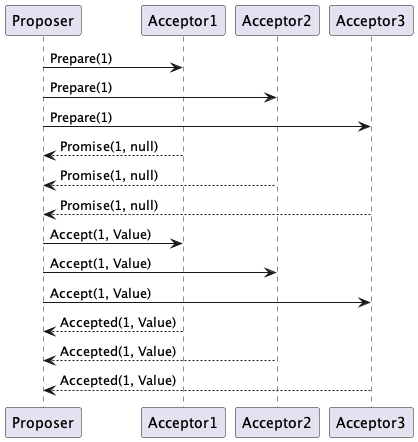
\includegraphics[width=0.55\textwidth]{fig/uml/paxos-default}
  \caption{Einfach Paxos als Beispielsequenze}
  \label{fig:simple-paxos}
\end{figure}


In diesem Diagramm sendet der Antragsteller (Proposer) zuerst eine Prepare-Anfrage an alle Akzeptoren. Die Akzeptoren antworten mit einem Versprechen (Promise). Dann sendet der Antragsteller eine Accept-Anfrage an alle Akzeptoren. Schließlich antworten die Akzeptoren mit einer Accepted-Nachricht, die signalisiert, dass sie den Vorschlag akzeptiert haben.

Paxos, obwohl es ein robustes und effizientes Protokoll ist, ist nicht ohne seine Herausforderungen. Es gibt mehrere kritische Szenarien, die bei der Anwendung des Paxos-Protokolls auftreten können.
\begin{itemize}
\item Netzwerklatenz und -ausfälle: Paxos kann durch Netzwerklatenz und -ausfälle erheblich gestört werden. Da Paxos auf der Kommunikation zwischen Prozessen basiert, können Verzögerungen und Ausfälle im Netzwerk dazu führen, dass Nachrichten verspätet oder gar nicht ankommen. Dies kann dazu führen, dass das Protokoll in einen unbestimmten Zustand gerät, in dem kein Konsens erreicht werden kann.
\item Konkurrierende Antragsteller: Ein weiteres kritisches Szenario tritt auf, wenn es mehrere konkurrierende Antragsteller gibt, die gleichzeitig versuchen, einen Konsens zu erreichen. Wenn jeder Antragsteller ständig neue Vorschläge mit höheren Nummern erzeugt, kann das System in einen Zustand geraten, der als \enquote{Livestream} bezeichnet wird, in dem kein Vorschlag jemals von einer Mehrheit der Akzeptoren akzeptiert wird.
\item Prozessausfälle: Da Paxos in verteilten Systemen eingesetzt wird, können Prozessausfälle ein ernsthaftes Problem darstellen. Wenn ein Antragsteller oder ein Akzeptor ausfällt, kann das den Fortschritt des Protokolls behindern. Paxos kann zwar Ausfälle tolerieren und sich erholen, aber der Ausfall kann dennoch zu Verzögerungen bei der Erreichung des Konsenses führen.
\end{itemize}

Um diese Szenarien in einer Sequenz zu illustrieren, können wir das vorherige Diagramm modifizieren, um die Auswirkungen von Netzwerk- und Prozessausfällen zu zeigen:


\begin{figure}[!ht]
  \centering
  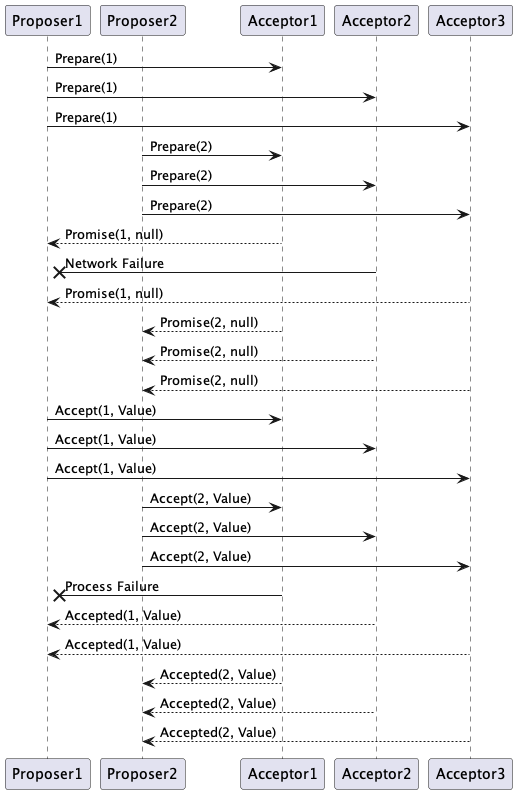
\includegraphics[width=0.65\textwidth]{fig/uml/paxos-issue}
  \caption{Komplexeres Paxos Beispiel}
  \label{fig:simple-paxos-issue}
\end{figure}

In diesem Diagramm sehen Sie, dass der Proposer1 eine Prepare-Anfrage an alle Akzeptoren sendet, aber die Anfrage an Acceptor2 scheitert aufgrund eines Netzwerkausfalls. Zur gleichen Zeit sendet Proposer2 auch Prepare-Anfragen, die alle erfolgreich sind. Proposer1 und Proposer2 senden dann ihre Accept-Anfragen, aber die Anfrage von Proposer1 an Acceptor1 scheitert wegen eines Prozessausfalls. Schließlich akzeptieren die Akzeptoren die Vorschläge von Proposer1 und Proposer2, aber aufgrund der Ausfälle gibt es keine Mehrheit, die einen einzigen Vorschlag akzeptiert, wodurch der Konsensprozess blockiert wird.

In der Realität würde in diesem kritischen Szenario Proposer1 den Konsens nicht erreichen, weil seine Accept-Anfrage an Acceptor1 aufgrund eines Prozessausfalls scheitert. Gleichzeitig würde Proposer2 erfolgreich Konsens erreichen, weil seine Accept-Anfragen von der Mehrheit der Akzeptoren akzeptiert werden.

Um die Situation zu beheben, könnte Proposer1 eine neue Runde mit einer höheren Vorschlagsnummer starten. Aber das würde zu weiterem Wettbewerb zwischen den Antragstellern führen und könnte das System in einen Zustand des \enquote{Livestreams} versetzen, in dem kein Konsens erreicht wird. Dieses Problem könnte durch den Einsatz eines Koordinators oder durch die Anwendung von Verzögerungen zur Begrenzung der Häufigkeit, mit der Antragsteller neue Runden starten, gemildert werden.

\begin{figure}[!htp]
  \centering
  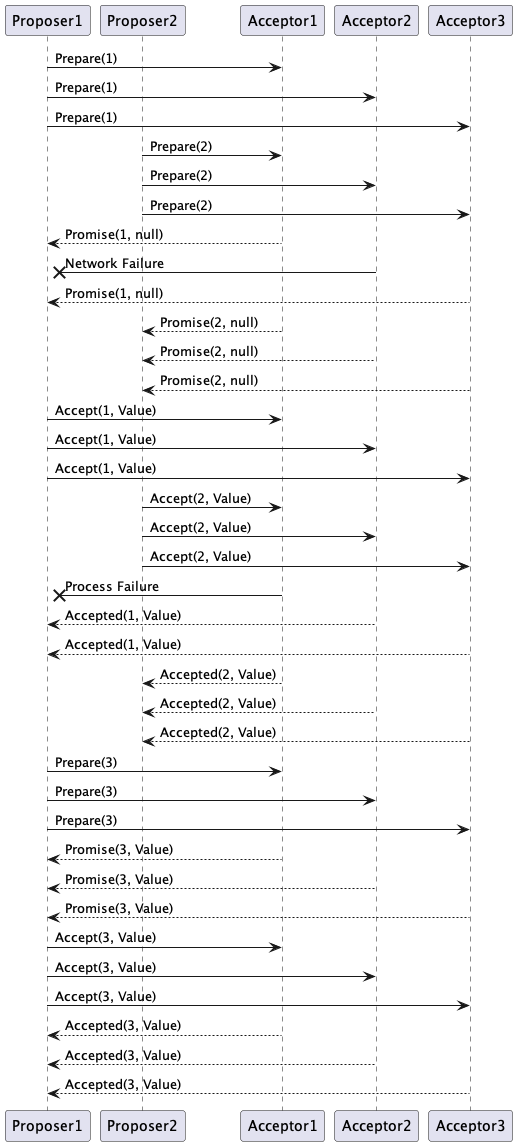
\includegraphics[width=0.65\textwidth]{fig/uml/paxos-issue-solve}
  \caption{Korrigiertes Paxos}
  \label{fig:simple-paxos-solve}
\end{figure}

In diesem Diagramm startet Proposer1 nach dem Ausfall eine neue Runde mit einer höheren Vorschlagsnummer und erreicht schließlich den Konsens.



\subsubsection{RAFT}\footnote{\url{https://www.youtube.com/watch?v=ro2fU8_mr2w}}

Das RAFT-Protokoll ist ein Konsensalgorithmus, der als Alternative zu Paxos entwickelt wurde. RAFT wurde entworfen, um die gleiche Funktionalität wie Paxos zu bieten, aber mit einem stärkeren Fokus auf Verständlichkeit und einfacher Implementierung.

Die wesentlichen Sequenzen in RAFT umfassen folgende Phasen:
\begin{itemize}
\item Wahl des Leaders: In RAFT gibt es immer einen Leader, der für die Koordination der Replikation verantwortlich ist. Wenn ein Knoten feststellt, dass es keinen Leader gibt (zum Beispiel, weil es keine Heartbeats vom Leader empfängt), beginnt es eine Wahl, indem es eine Anfrage zur Wahl an alle anderen Knoten sendet. Die Knoten stimmen für den ersten Kandidaten, der eine Anfrage sendet, und der Kandidat, der die meisten Stimmen erhält, wird zum neuen Leader.
\item Log-Replikation: Nachdem ein Leader gewählt wurde, beginnt der Prozess der Log-Replikation. Der Leader nimmt Anfragen von Clients entgegen, fügt sie seinem Log hinzu und sendet dann AppendEntries-Anfragen an die Follower, um das Log zu replizieren. Die Follower antworten dem Leader, wenn sie die Einträge erfolgreich repliziert haben.
\item Commit: Sobald der Leader feststellt, dass eine Mehrheit der Follower einen Log-Eintrag repliziert hat, erklärt er den Eintrag für committed und wendet den Eintrag auf seinen Zustand an. Der Leader informiert die Follower über committed Einträge durch nachfolgende AppendEntries-Anfragen.
\end{itemize}
Um diese Sequenzen in einer Sequenz zu illustrieren, wurde  das Diagramm XY angefertigt. In diesem Diagramm wird der Prozess der Leaderwahl, Log-Replikation und Commit in RAFT dargestellt.


\subsubsection{ZAB}
ZooKeeper Atomic Broadcast (ZAB) ist ein Konsensprotokoll, das von Apache ZooKeeper verwendet wird. Es ist darauf ausgelegt, eine geordnete, zuverlässige und atomare Übertragung von Nachrichten zwischen den Knoten eines verteilten Systems zu ermöglichen. Das ZAB-Protokoll hat zwei Hauptmodi: einen Erholungsmodus, der nach dem Ausfall eines Leaders ausgeführt wird, und einen Broadcast-Modus, der ausgeführt wird, wenn das System stabil ist.

Die wesentlichen Sequenzen von ZAB umfassen folgende Phasen:
\begin{itemize}
\item Führungsfindung (Leader Election): Wenn ein Leader ausfällt oder wenn das System zum ersten Mal startet, müssen die Knoten (die als \enquote{ZooKeeper Server} bezeichnet werden) einen neuen Leader wählen. Dies geschieht in der Phase der Führungsfindung, in der jeder Knoten einen Vorschlag mit seiner gewählten Führungsnummer (Epochennummer) und seiner eigenen Server-ID sendet. Der Knoten mit der höchsten gewählten Führungsnummer wird zum Leader.
\item Synchronisation: Nachdem ein Leader gewählt wurde, muss das System synchronisiert werden, um sicherzustellen, dass alle Knoten denselben Zustand haben. Der neue Leader sendet dazu seinen Zustand an alle anderen Knoten (Follower). Wenn ein Follower einen Zustand empfängt, der neuer als sein eigener ist, aktualisiert er seinen Zustand, um mit dem Leader übereinzustimmen.
\item Broadcast: Sobald das System synchronisiert ist, kann der Leader beginnen, Updates zu senden. Diese Updates werden als \enquote{Vorschläge} bezeichnet und enthalten eine eindeutige Transaktions-ID, die aus der Führungsnummer und einer fortlaufenden Sequenznummer besteht. Die Follower akzeptieren diese Vorschläge und fügen sie ihrem jeweiligen Zustand hinzu.
\end{itemize}

ZAB  ist somit  ein zuverlässiges, geordnetes und fehlertolerantes Protokoll, das dazu dient, Transaktionen auf mehrere Server zu verteilen, um eine fehlertolerante, verteilte Koordination zu ermöglichen. Es ist das zugrunde liegende Protokoll, das Apache ZooKeeper verwendet.

Im ZAB-Protokoll wird ein Leader-basiertes Multicast-Modell verwendet. In diesem Modell wird ein Knoten zum Leader gewählt, und dieser Leader ist verantwortlich für das Senden von Aktualisierungen an alle anderen Knoten (Follower) im Cluster. Der Leader garantiert die Reihenfolge der Nachrichten, was dazu beiträgt, eine \enquote{totale Ordnung} zu etablieren. Das bedeutet, dass alle Operationen, die im System auftreten, in einer konsistenten, vorhersehbaren Reihenfolge auftreten.

Dieses Modell ist zuverlässig, weil es sicherstellt, dass alle Nachrichten, die vom Leader gesendet werden, von den Followern empfangen werden. Wenn ein Follower eine Nachricht nicht empfängt, wird die Nachricht erneut gesendet, bis der Follower bestätigt, dass er sie empfangen hat.

Zusätzlich zur totalen Ordnung der vom Leader umgesetzten Nachrichten  unterstützt ZAB auch die kausale Ordnung der Operationen auf den Daten. Das bedeutet, dass wenn eine Operation A eine andere Operation B verursacht, Operation A immer vor Operation B in der Sequenz der Operationen auftreten wird.

In ZooKeeper sind die Garantien, die durch ZAB ermöglicht werden, sequenziell konsistent und atomar im Single Node Image. Das bedeutet, dass jede Operation, die auf einem Knoten ausgeführt wird, genau so aussieht, als ob sie auf einem einzelnen System ausgeführt wurde, und dass sie entweder vollständig ausgeführt wird oder überhaupt nicht.

ZooKeeper ermöglicht auch zeitnahe Operationen, wie das Erstellen, Löschen und Abrufen von Daten, sowie das Abrufen von Kindknoten. Diese Operationen werden in einem hierarchischen Namensraum ausgeführt, der es Entwicklern ermöglicht, Ressourcen auf eine strukturierte und organisierte Weise zu verwalten.

ZooKeeper bietet eine Vielzahl von Funktionen, die für verteilte Systeme tels unerlässlich sind, wie z.B.:
\begin{itemize}
\item Locks: ZooKeeper kann verwendet werden, um exklusive Sperren in einem verteilten System zu implementieren. Dies ist nützlich, wenn nur ein Prozess zu einem bestimmten Zeitpunkt eine Ressource verwenden darf.
\item Leader Election: In einigen verteilten Systemen kann es nötig sein, einen Prozess auszuwählen, der bestimmte Aufgaben ausführt. ZooKeeper kann verwendet werden, um diesen Leader auf einer fairen und transparenten Weise zu wählen.
\item Configuration Management: ZooKeeper kann verwendet werden, um Konfigurationsinformationen auf einer zentralen Stelle zu speichern und zu verteilen. Dies ist nützlich, um sicherzustellen, dass alle Prozesse in einem verteilten System die gleiche Konfiguration verwenden.
\end{itemize}

Das ZAB-Protokoll spielt dabei eine Schlüsselrolle, da es die konsistente und zuverlässige Ausführung dieser Funktionen ermöglicht. Durch die Verwendung von Leader-basiertem Multicast und der Gewährleistung von totaler und kausaler Ordnung stellt ZAB sicher, dass alle Prozesse in einem verteilten System eine konsistente Sicht auf die Daten haben.

Um zuverlässigen Datenverkehr zu gewährleisten, verwendet ZAB ein Zwei-Phasen-Commit-Protokoll, welches aus den Dantenbankgrundlagen bekannt sein sollte. Wenn ein Leader eine Aktualisierung vorschlägt, sendet er zunächst einen Vorschlag an alle Follower. Die Follower antworten dann mit einer Bestätigung, dass sie den Vorschlag erhalten haben. Erst wenn der Leader Bestätigungen von einer Mehrheit der Follower erhalten hat, kann er die Aktualisierung abschließen und an alle Follower senden.

All dies zusammen ermöglicht es ZooKeeper, eine konsistente und zuverlässige Koordination in verteilten Systemen zu gewährleisten. Es stellt sicher, dass alle Prozesse die gleiche Sicht auf die Daten haben und dass alle Operationen in einer konsistenten und vorhersehbaren Reihenfolge ausgeführt werden. 

\subsubsection{Konsens mit Crash Failures}
Die \enquote{Unmöglichkeit von 1-Crash-Konsens} in verteilten Systemen bezieht sich auf einen fundamentalen Beweis in der Theorie verteilter Systeme, der ursprünglich von Michael J. Fischer, Nancy A. Lynch und Michael S. Paterson in ihrem 1985 veröffentlichten Artikel \enquote{Impossibility of Distributed Consensus with One Faulty Process} vorgebracht wurde. Dieser Beweis wird oft als FLP-Unmöglichkeitstheorem bezeichnet.

Die grundlegende Aussage dieses Beweises ist, dass es in einem asynchronen verteilten System mit nur einem möglicherweise fehlerhaften Prozess (d.h. einem Prozess, der abstürzen kann) keinen deterministischen Algorithmus geben kann, der immer zu einem Konsens führt. Ein asynchrones System ist ein System, in dem es keine festen Obergrenzen für die Zeit gibt, die zum Senden von Nachrichten oder zum Ausführen von Schritten in einem Algorithmus benötigt wird.

Der Beweis nutzt die Tatsache, dass in einem asynchronen System immer die Möglichkeit besteht, dass ein Prozess oder eine Nachricht unendlich verzögert wird. Dies kann dazu führen, dass die anderen Prozesse nicht in der Lage sind, zu bestimmen, ob ein Prozess abgestürzt ist oder einfach nur verzögert wird. Daher kann es Fälle geben, in denen das System nicht in der Lage ist, einen Konsens zu erreichen, da es immer Unsicherheit darüber gibt, ob alle Prozesse ihren Zustand gemeldet haben oder nicht.

Dieses Ergebnis hat tiefgreifende Auswirkungen auf die Art und Weise, wie wir verteilte Systeme entwerfen und verstehen. Es zeigt, dass wir in bestimmten Fällen Kompromisse eingehen müssen, zum Beispiel indem wir die Asynchronität einschränken oder nichtdeterministische Algorithmen verwenden, um Konsens zu erreichen.

Die FLP-Unmöglichkeitsergebnisse haben zu einem tiefgreifenden Verständnis der Herausforderungen bei der Entwicklung von Algorithmen für verteilte Systeme geführt, insbesondere solchen, die Asynchronität und Fehler tolerieren müssen.

Die Schlussfolgerungen des FLP-Theorems haben die Forschung in mehrere Richtungen gelenkt:
\begin{itemize}
\item Teilsynchrone Systeme: In der Praxis sind Systeme selten völlig asynchron. Es gibt oft zumindest einige Grenzen für die Zeit, die Prozesse und Nachrichten benötigen. Dies hat zur Entwicklung von Konsensalgorithmen für teilsynchrone Systeme geführt, in denen bestimmte zeitliche Einschränkungen gelten, auch wenn sie recht locker sein können.
\item Randomisierte Algorithmen: Während das FLP-Ergebnis für deterministische Algorithmen gilt, ist es möglich, Konsens in einem asynchronen System zu erreichen, wenn wir Zufallszahlen einsetzen. Ein Beispiel für einen solchen Algorithmus ist der Randomized Consensus Algorithmus.
\item Praktische Konsensalgorithmen: Trotz des FLP-Unmöglichkeitsergebnisses wurden mehrere praktische Konsensalgorithmen für verteilte Systeme entwickelt, darunter Paxos, Raft und Zab. Diese Algorithmen sind entworfen, um in realen Systemen gut zu funktionieren, auch wenn sie in extrem asynchronen Szenarien oder bei bestimmten Arten von Netzwerkpartitionen scheitern können.
\end{itemize}
Es ist wichtig zu beachten, dass das FLP-Unmöglichkeitsergebnis spezifisch für asynchrone, unzuverlässige Systeme gilt. In einem synchronen System, in dem es feste Obergrenzen für die Zeit gibt, die Prozesse und Nachrichten benötigen, ist es möglich, einen Konsens zu erreichen, selbst wenn einige Prozesse abstürzen können. Gleiches gilt für asynchrone Systeme, in denen alle Prozesse zuverlässig sind. Das FLP-Ergebnis zeigt jedoch, dass die Kombination von Asynchronität und Unzuverlässigkeit zu grundlegenden Schwierigkeiten bei der Erzielung eines Konsenses führt.

Sowohl Bracha-Toueg als auch Chandra-Toueg sind Algorithmen, die versuchen, den Konsens in verteilten Systemen trotz der Einschränkungen, die durch das FLP-Unmöglichkeitsergebnis hervorgehoben wurden, zu erreichen. Beide Algorithmen nutzen das Konzept der teilweisen Synchronität, bei dem einige Obergrenzen für die Kommunikations- und Verarbeitungszeiten existieren, auch wenn diese Grenzen recht locker sind.
\begin{itemize}
\item Bracha-Toueg Crash Consensus: Dies ist ein Algorithmus für den binären Konsens in einem teilweise synchronen Modell, bei dem jeder Prozess entweder abstürzen kann (d.h., er kann zu irgendeinem Zeitpunkt aufhören, Aktionen auszuführen) oder korrekt ist. Der Bracha-Toueg-Algorithmus garantiert sowohl Sicherheit (d.h., alle korrekten Prozesse einigen sich auf den gleichen Wert, und wenn alle korrekten Prozesse den gleichen anfänglichen Wert haben, dann einigen sie sich auf diesen Wert) als auch Liveness (d.h., alle korrekten Prozesse entscheiden sich schließlich), solange mehr als zwei Drittel der Prozesse korrekt sind.
\item Chandra-Toueg Unreliable Failure Detectors: Dieser Ansatz konzentriert sich auf die Implementierung von Konsensalgorithmen in asynchronen Systemen mithilfe von sogenannten unzuverlässigen Fehlerdetektoren. Ein unzuverlässiger Fehlerdetektor ist ein Mechanismus, der die Möglichkeit hat, fehlerhafte Prozesse zu erkennen, aber Fehler machen kann, zum Beispiel indem er einen korrekten Prozess fälschlicherweise als fehlerhaft markiert. Chandra und Toueg zeigten, dass es möglich ist, mit solchen unzuverlässigen Fehlerdetektoren einen Konsens zu erzielen, auch in vollständig asynchronen Systemen.
\end{itemize}    

Unzuverlässige Fehlerdetektoren sind eine zentrale Komponente in vielen Algorithmen für verteilte Systeme, insbesondere in Konsensalgorithmen. Sie stellen eine Abstraktion dar, die es den Prozessen in einem verteilten System ermöglicht, zu erahnen, ob andere Prozesse abgestürzt sind.

Es ist wichtig zu beachten, dass Fehlerdetektoren als \enquote{unzuverlässig} bezeichnet werden, weil sie in asynchronen Systemen nicht perfekt sein können. In einem asynchronen System kann ein Prozess, der sehr langsam ist oder dessen Nachrichten stark verzögert werden, von anderen Prozessen als abgestürzt wahrgenommen werden, auch wenn er tatsächlich noch läuft.

Ein einfaches Beispiel für einen unzuverlässigen Fehlerdetektor ist ein Timeout-basierter Fehlerdetektor. In diesem Szenario würde jeder Prozess regelmäßig \enquote{Herzschlag}-Nachrichten an die anderen Prozesse senden. Wenn ein Prozess für eine bestimmte Zeit keine Herzschlag-Nachricht von einem anderen Prozess erhält, könnte er annehmen, dass dieser Prozess abgestürzt ist und ihn als solchen markieren.

Allerdings könnte ein sehr langsamer Prozess oder Netzwerkverzögerungen dazu führen, dass ein Prozess fälschlicherweise als abgestürzt markiert wird, wenn er tatsächlich noch funktioniert - daher die Bezeichnung \enquote{unzuverlässig}.

\subsubsection{Konsens mit Byzantine Failures}
In verteilten Systemen bezieht sich ein \enquote{byzantinischer Fehler} auf einen Fehler, der dazu führt, dass ein Knoten (oder Prozess) in einem System auf eine unvorhersehbare, unzuverlässige oder gar bösartige Weise reagiert. Der Begriff geht auf das berühmte \enquote{Byzantinische Generäle Problem} zurück, das ursprünglich in einem Artikel von Leslie Lamport, Robert Shostak und Marshall Pease aus dem Jahr 1982 formuliert wurde.

Das \enquote{Byzantinische Generäle Problem} ist ein Analogon zu den Herausforderungen, die bei der Koordination und dem Erreichen eines Konsenses in einem verteilten System auftreten, in dem einige der Knoten fehlerhaft sein könnten. Insbesondere müssen die \enquote{loyalen} Generäle (analog zu den korrekten Knoten in einem verteilten System) eine gemeinsame Strategie festlegen, trotz der Möglichkeit, dass einige der Generäle \enquote{Verräter} sein könnten und versuchen könnten, die loyale Koordination zu stören.

In einem verteilten System kann ein byzantinischer Knoten falsche oder inkonsistente Informationen an die anderen Knoten senden, kann scheinbar abstürzen und dann wieder auftauchen, oder kann auf andere Weise versuchen, die korrekte Funktion des Systems zu stören. Ein byzantinischer Fehler ist daher schwieriger zu handhaben als einfache Crash-Fehler, bei denen ein Knoten einfach aufhört zu reagieren.

Es wurde gezeigt, dass das Erreichen eines Konsenses in einem verteilten System mit byzantinischen Fehlern nur möglich ist, wenn mehr als zwei Drittel der Knoten korrekt sind. Es gibt verschiedene Algorithmen, die versuchen, dies zu erreichen, einschließlich der ursprünglichen Lösung, die in dem Artikel über die byzantinischen Generäle vorgeschlagen wurde, sowie späterer Algorithmen wie Practical Byzantine Fault Tolerance (PBFT).

Die Fähigkeit, byzantinische Fehler zu tolerieren, ist besonders wichtig in offenen, dezentralisierten Systemen wie Blockchains, in denen Knoten möglicherweise einen Anreiz haben, das System zu betrügen oder zu stören. Daher sind byzantinische Konsensalgorithmen ein aktiver Bereich der Forschung und Entwicklung in solchen Systemen. Neben PBFT werden die genannten Verfahren um Proof of Work oder auch Proof of Stake wieder relevant.  

\subsection{Koordination}

Die Koordination in verteilten Systemen ist eine wichtige Herausforderung, da einzelne Komponenten unabhängig voneinander agieren und Informationen austauschen müssen, um gemeinsame Ziele zu erreichen. Es gibt verschiedene Ansätze und Techniken, um die Koordination zu ermöglichen. Im Folgenden wird eine Einführung in die Koordination mittels Algorithmen geben:

\subsubsection{Waves}
Wave-Algorithmen sind eine Klasse von Algorithmen in der Graphentheorie und werden oft in verteilten Systemen eingesetzt. Sie zeichnen sich dadurch aus, dass sie Informationen über Graphen (oder Netzwerke) verteilen, ähnlich wie Wellen sich in einem physischen Medium ausbreiten. Diese Algorithmen werden typischerweise zur Lösung von Problemen wie dem Erkennen von Knoten, der Synchronisation von Prozessen, der Suche nach kürzesten Pfaden, der Auffindung von Toten Knoten und der Bestimmung von Grapheneigenschaften eingesetzt.

Die Grundidee bei Wave-Algorithmen ist, dass ein Knoten eine \enquote{Welle} (in Form einer Nachricht) an seine Nachbarn sendet und diese Welle sich dann durch den Graphen ausbreitet, bis alle Knoten erreicht sind. Während dieser Ausbreitung kann jeder Knoten, der die Welle erhält, eine bestimmte Aktion ausführen, wie zum Beispiel seinen Zustand aktualisieren oder Informationen an die Welle anhängen.

Ein einfacher Beispiel-Wave-Algorithmus könnte wie folgt aussehen:
\begin{itemize}
\item Ein Startknoten sendet eine Welle an alle seine Nachbarn.
\item Jeder Knoten, der die Welle erhält, führt eine bestimmte Aktion aus (zum Beispiel aktualisiert er einen Zähler oder speichert eine Information) und sendet die Welle an alle seine Nachbarn, die die Welle noch nicht erhalten haben.
\item Dieser Prozess wiederholt sich, bis alle Knoten im Graphen die Welle erhalten und verarbeitet haben.
\end{itemize}
Es gibt viele verschiedene Varianten von Wave-Algorithmen, abhängig von den spezifischen Anforderungen des Problems, das gelöst werden soll. Einige Wave-Algorithmen können zum Beispiel mehrere Wellen gleichzeitig senden, während andere spezielle Techniken verwenden können, um die Ausbreitung der Welle zu steuern und zu optimieren.

Wave-Algorithmen können in einer Vielzahl von Anwendungen eingesetzt werden, einschließlich Netzwerk-Routing, Synchronisation von verteilten Systemen, Erkennung von Knoten und Verteilung von Ressourcen in einem Netzwerk. In all diesen Fällen ermöglichen sie eine effiziente und dezentralisierte Lösung, die gut auf große und dynamische Systeme skaliert.

Traversal-, Tree- und Echo-Algorithmen sind spezielle Klassen von Wave-Algorithmen, die in verteilten Systemen eingesetzt werden, um bestimmte Aufgaben auszuführen. Hier ist eine kurze Beschreibung und ein Vergleich der drei:
\begin{itemize}
\item Traversal-Algorithmus (Graph-Durchlauf-Algorithmus): \\Traversal-Algorithmen werden verwendet, um alle Knoten in einem Graphen zu besuchen. Das bekannteste Beispiel für diese Art von Algorithmen sind Tiefensuche (Depth-First Search, DFS) und Breitensuche (Breadth-First Search, BFS). Beide Algorithmen beginnen bei einem bestimmten Knoten und besuchen alle anderen Knoten durch \enquote{Wandern} entlang der Kanten des Graphen. DFS macht dies, indem es so weit wie möglich entlang jeder Verzweigung geht, bevor es zurückkehrt, während BFS alle Nachbarn eines Knotens besucht, bevor es zu den Nachbarn der Nachbarn geht. Diese Algorithmen sind hilfreich bei Aufgaben wie dem Finden eines Pfades zwischen zwei Knoten, dem Testen, ob ein Graph zusammenhängend ist, oder dem Finden von Kreisen in einem Graphen.
\item Tree-Algorithmus (Baumalgorithmus): \\Tree-Algorithmen sind eine spezielle Klasse von Traversal-Algorithmen, die dazu dienen, einen Spannbaum (einen Baum, der alle Knoten des Graphen verbindet, aber keine Kreise enthält) aus einem Graphen zu erzeugen. Ein bekanntes Beispiel ist der Algorithmus von Prim oder Kruskal, der verwendet wird, um einen minimalen Spannbaum zu erzeugen. Diese Art von Algorithmen kann besonders nützlich sein in Netzwerken, um redundante Verbindungen zu entfernen und dennoch sicherzustellen, dass alle Knoten miteinander verbunden sind.
\item Echo-Algorithmus: \\Der Echo-Algorithmus ist ein spezieller Wave-Algorithmus, der dazu dient, Informationen über ein verteiltes System zu sammeln und an einen zentralen Knoten zurückzusenden. Ein Knoten sendet eine Anfrage an alle seine Nachbarn und wartet auf deren Antworten. Wenn ein Knoten eine Anfrage erhält, sendet er die Anfrage weiter an alle seine Nachbarn und wartet auf deren Antworten. Sobald ein Knoten alle Antworten von seinen Nachbarn erhalten hat, verarbeitet er die Antworten und sendet eine einzige Antwort an den Knoten, von dem er die ursprüngliche Anfrage erhalten hat. Dieser Algorithmus wird oft verwendet, um Informationen wie die Gesamtzahl der Knoten in einem Netzwerk, den kürzesten Pfad zu einem bestimmten Knoten oder die Verfügbarkeit von Ressourcen zu sammeln.
\end{itemize}
Alle Algorithmen bieten jeweils verschiedene Methoden zur Verarbeitung und Sammlung von Informationen in einem Netzwerk, abhängig von den spezifischen Anforderungen der Aufgabe.

\subsubsection{Snapshot}

Snapshot-Algorithmen sind eine Art von Algorithmen in verteilten Systemen, die dazu verwendet werden, den globalen Zustand des Systems zu einem bestimmten Zeitpunkt zu erfassen. Diese Algorithmen sind besonders nützlich in Systemen, in denen verschiedene Prozesse gleichzeitig und unabhängig voneinander ausgeführt werden, da sie es ermöglichen, einen konsistenten \enquote{Schnappschuss} des Zustands aller Prozesse zu erstellen.

Es gibt verschiedene Snapshot-Algorithmen, aber einer der bekanntesten ist der Chandy-Lamport-Algorithmus. Dieser Algorithmus wurde 1985 von K. Mani Chandy und Leslie Lamport entwickelt. Der Algorithmus ermöglicht es, einen globalen Zustand eines verteilten Systems zu erfassen, der konsistent ist hinsichtlich \enquote{happen-before} Beziehungen zwischen Ereignissen.

Hier ist eine vereinfachte Beschreibung des Chandy-Lamport-Algorithmus:
\begin{itemize}
\item Ein Prozess, der einen globalen Zustandsschnappschuss initiieren möchte (wir nennen ihn Initiator), speichert seinen eigenen Zustand und sendet spezielle Marker-Nachrichten an alle anderen Prozesse, mit denen er kommuniziert.
\item Wenn ein Prozess eine Marker-Nachricht erhält und es ist das erste Mal, dass er einen Marker für diesen Schnappschuss erhält, speichert er seinen aktuellen Zustand und sendet Marker-Nachrichten an alle anderen Prozesse, mit denen er kommuniziert. Außerdem beginnt er, alle eingehenden Nachrichten auf jedem Kanal zu speichern, bis er einen Marker auf diesem Kanal erhält.
\item Wenn ein Prozess eine Marker-Nachricht auf einem Kanal erhält und er hat bereits seinen Zustand für diesen Schnappschuss gespeichert, stoppt er die Aufzeichnung der Nachrichten auf diesem Kanal.
\end{itemize} 
Nachdem der Algorithmus ausgeführt wurde, besteht der Schnappschuss aus dem gespeicherten Zustand jedes Prozesses und den gespeicherten Nachrichten auf jedem Kanal. Dieser Schnappschuss ist konsistent im Sinne von \enquote{happen-before} Beziehungen: Wenn ein Ereignis A vor einem Ereignis B auftritt, dann wird, wenn der Schnappschuss nach B aufgenommen wird, auch A im Schnappschuss enthalten sein.


Neben dem Chandy-Lamport-Algorithmus existieren andere Algorithmen, wie der Lai-Yang-Algorithmus. Dieser unterscheidet sich jedoch in der Art und Weise, wie er das Ziel erreicht.

Der Chandy-Lamport-Algorithmus setzt auf die Verwendung von Marker-Nachrichten, die zwischen den Prozessen hin und her geschickt werden, um den Start- und Endpunkt der Schnappschusserfassung zu signalisieren. Wenn ein Prozess eine Marker-Nachricht erhält, speichert er seinen Zustand und leitet die Marker-Nachricht an alle seine Ausgangskanäle weiter. Dieser Prozess wird fortgesetzt, bis alle Prozesse ihren Zustand gespeichert und alle Marker-Nachrichten erhalten haben. Ein wichtiger Aspekt dieses Algorithmus ist, dass er einen synchronisierten Startpunkt erfordert, aber keinen synchronisierten Endpunkt.

Der Lai-Yang-Algorithmus hingegen ist ein sogenannter \enquote{farbiger} Algorithmus. In diesem Kontext bedeutet \enquote{farbig}, dass Nachrichten und Prozesse entweder als \enquote{rot} oder \enquote{weiß} markiert sind. Zu Beginn des Algorithmus sind alle Prozesse und Nachrichten weiß. Wenn ein Prozess beschließt, einen Schnappschuss zu starten, wird er rot und speichert seinen Zustand. Es sendet dann rote Nachrichten an alle anderen Prozesse. Ein Prozess, der eine rote Nachricht erhält, speichert seinen Zustand und wird ebenfalls rot. 
Im Detail ist der Algorithmus wie folgt:
\begin{itemize}
\item Initialisierung: Zu Beginn des Algorithmus sind alle Prozesse und Nachrichten weiß.
\item Start des Snapshots: Ein beliebiger Prozess kann die Aufnahme eines Schnappschusses initiieren. Dieser Prozess ändert seine Farbe von Weiß zu Rot, speichert seinen lokalen Zustand und beginnt, rote Nachrichten zu senden.
\item Aufnahme des Zustands: Wenn ein weißer Prozess eine rote Nachricht empfängt, ändert er seine Farbe zu Rot, speichert seinen lokalen Zustand und beginnt, rote Nachrichten zu senden. Wenn ein roter Prozess eine rote Nachricht empfängt, ändert er nichts an seinem Zustand, sondern sendet weiterhin rote Nachrichten.
\item Ende des Snapshots: Der globale Zustand des Systems ist erfasst, sobald alle Prozesse rot geworden sind und alle weißen Nachrichten aus dem System entfernt wurden. Da alle roten Prozesse nur rote Nachrichten senden, werden alle Nachrichten, die nach dem Snapshot empfangen werden, ebenfalls rot sein.
\end{itemize}

Es ist wichtig zu beachten, dass dieser Algorithmus auch sicherstellt, dass der erfasste globale Zustand des Systems konsistent ist, d.h., er respektiert die \enquote{happen-before}-Beziehungen zwischen den Ereignissen im System.  Der Vorteil dieses Algorithmus besteht darin, dass er keinen synchronisierten Startpunkt erfordert, was ihn flexibler macht als den Chandy-Lamport-Algorithmus. Allerdings kann er mehr Ressourcen verbrauchen, insbesondere in Systemen mit vielen Prozessen und Nachrichten.

Anwendungen von Snapshot-Algorithmen sind:
\begin{itemize}
\item Deadlock-Erkennung: Snapshot-Algorithmen können verwendet werden, um Deadlocks in verteilten Systemen zu erkennen. Durch die Erfassung des globalen Zustands des Systems kann ein Prozess bestimmen, ob es eine Zyklusabhängigkeit zwischen Prozessen gibt, was auf einen Deadlock hindeuten würde.
\item Globales Checkpointing: In verteilten Systemen kann ein globaler Schnappschuss dazu verwendet werden, einen Zustand zu erzeugen, zu dem das System nach einem Ausfall zurückkehren kann. Dies ist nützlich, um die Ausfallerholung zu erleichtern und den Datenverlust zu minimieren.
\item Eventuelle Konsistenz: Snapshot-Algorithmen können verwendet werden, um sicherzustellen, dass eine verteilte Datenbank im Laufe der Zeit eine konsistente Ansicht der Daten erreicht. Mit anderen Worten, sie können dazu beitragen, sicherzustellen, dass alle Repliken eines Datenelements schließlich denselben Wert haben.
\item Monitoring und Debugging: In verteilten Systemen kann es eine Herausforderung sein, die Interaktionen zwischen den verschiedenen Prozessen zu verstehen, insbesondere wenn Probleme auftreten. Durch die Aufnahme eines globalen Schnappschusses des Systems zu einem bestimmten Zeitpunkt können Entwickler oder Systemadministratoren den Zustand jedes Prozesses und die Nachrichten, die zwischen den Prozessen ausgetauscht werden, überprüfen. Dies kann dabei helfen, das Problem zu identifizieren und zu beheben.
\item Simulation von verteilten Systemen: Snapshot-Algorithmen können auch in der Simulation von verteilten Systemen nützlich sein. Durch die Aufnahme von Schnappschüssen des Systems zu verschiedenen Zeitpunkten können Wissenschaftler das Verhalten des Systems unter verschiedenen Bedingungen analysieren und besser verstehen.
\item Konsistenz in verteilten Datenbanken: Snapshot-Algorithmen können dazu beitragen, konsistente Lesevorgänge in verteilten Datenbanken zu ermöglichen, indem sie eine konsistente Ansicht der Datenbank zu einem bestimmten Zeitpunkt erzeugen. Dies ist besonders wichtig in Systemen, die eine hohe Verfügbarkeit und Partitionstoleranz erfordern.
\end{itemize}

\subsubsection{Checkpoint}
Der Peterson-Kearns Rollback Recovery-Algorithmus unterscheidet sich von den beiden anderen Algorithmen, da er nicht nur darauf abzielt, den globalen Zustand eines Systems zu erfassen, sondern auch darauf, das System zu einem konsistenten Zustand zurückzusetzen, wenn ein Fehler auftritt. Er tut dies, indem er sogenannte \enquote{Checkpoints} oder gespeicherte Zustände der Prozesse verwendet. Wenn ein Fehler erkannt wird, wird das System zu dem Checkpoint zurückgesetzt, der unmittelbar vor dem Fehler auftrat. Dann wird das System von diesem Punkt aus neu gestartet, wobei alle Nachrichten, die nach dem Checkpoint empfangen wurden, erneut gesendet werden. Dieser Ansatz kann effektiv sein, um die Ausfallzeit in einem verteilten System zu minimieren, erfordert aber ein sorgfältiges Management der Checkpoints und der Nachrichtenwiederholung.
Im Detail ist der Algorithmus wie folgt:
\begin{itemize}
\item Checkpointing: Jeder Prozess im System führt in regelmäßigen Abständen ein lokales Checkpointing durch, bei dem der aktuelle Zustand des Prozesses gespeichert wird. Diese Checkpoints dienen als Wiederherstellungspunkte im Falle eines Fehlers.
\item Nachrichtenprotokollierung: Zusätzlich zum Checkpointing protokolliert jeder Prozess alle gesendeten und empfangenen Nachrichten. Dies ermöglicht es dem System, den genauen Zustand zum Zeitpunkt des letzten Checkpoints zu rekonstruieren.
\item Fehlererkennung: Wenn ein Fehler in einem Prozess erkannt wird, wird dieser Prozess und möglicherweise auch andere Prozesse, die von dem fehlerhaften Prozess abhängig sind, zu ihrem letzten Checkpoint zurückgerollt.
\item Nachrichtenwiederholung: Nach dem Rollback werden alle Nachrichten, die nach dem letzten Checkpoint gesendet wurden, aus dem Protokoll erneut gesendet. Dies stellt sicher, dass alle Prozesse, die von dem fehlerhaften Prozess abhängig sind, wieder in einen konsistenten Zustand gebracht werden.
\item Wiederherstellung: Nachdem alle Nachrichten wiederholt wurden, wird der Betrieb des Systems fortgesetzt.
\end{itemize}
Der Peterson-Kearns-Rollback-Recovery-Algorithmus hat den Vorteil, dass er es ermöglicht, das System nach einem Fehler schnell zu einem konsistenten Zustand zurückzusetzen. Dies kann dazu beitragen, die Ausfallzeit des Systems zu minimieren und den Datenverlust zu begrenzen. Allerdings erfordert dieser Ansatz ein sorgfältiges Management der Checkpoints und der Nachrichtenprotokollierung, und er kann zu einer erheblichen Wiederholung von Berechnungen führen, wenn Fehler auftreten.


\subsubsection{Deadlock Detection}

Deadlocks sind Situationen in verteilten Systemen (und auch in anderen Arten von Systemen), in denen zwei oder mehr Prozesse unbegrenzt auf Ressourcen warten, die von den anderen Prozessen gehalten werden. Deadlock-Erkennungsalgorithmen sind Verfahren, die entwickelt wurden, um diese Situationen zu identifizieren und gegebenenfalls zu beheben.

Ein grundlegender Ansatz zur Deadlock-Erkennung besteht darin, den Ressourcenzuteilungsgraphen des Systems zu überprüfen. Dieser Graph besteht aus Knoten, die Prozesse und Ressourcen darstellen, und Kanten, die die Beziehungen zwischen diesen Elementen (z.B. \enquote{Prozess P besitzt Ressource R} oder \enquote{Prozess P wartet auf Ressource R}) 
darstellen. Ein Deadlock tritt auf, wenn es in diesem Graphen einen Zyklus gibt. Das bedeutet, dass es eine Gruppe von Prozessen gibt, in der jeder Prozess auf eine Ressource wartet, die von einem anderen Prozess in der Gruppe gehalten wird.
Zur Erkennung von Deadlocks in verteilten Systemen gibt es verschiedene Algorithmentypen. Hier sind zwei gängige Methoden:

\begin{itemize}
\item Wait-for-Graphs-Algorithmus: Wait-for-Graphs sind eine gängige Methode zur Deadlock-Erkennung in Betriebssystemen und verteilten Systemen. Sie stellen die Abhängigkeiten zwischen Prozessen und Ressourcen dar. Knoten im Graphen repräsentieren Prozesse und Ressourcen, während Kanten die \enquote{wartet auf} Beziehungen darstellen. Wenn ein Prozess auf eine Ressource wartet, die von einem anderen Prozess gehalten wird, wird eine Kante von dem wartenden Prozess zum haltenden Prozess gezeichnet. Ein Zyklus in diesem Graphen deutet auf einen Deadlock hin, da jeder Prozess im Zyklus auf eine Ressource wartet, die von einem anderen Prozess im Zyklus gehalten wird. Dieser Algorithmus wird typischerweise in einem zentralisierten System verwendet, in dem ein einziger Koordinator den gesamten Wait-for-Graphen aufbewahrt und auf Deadlocks prüft. In einem verteilten System könnte ein ähnlicher Ansatz mit einem verteilten Graphen und einer koordinierten Zykluserkennung verwendet werden.
\item Konsensbasierte Algorithmen sind eine Art von Koordinationsmechanismus, der oft in verteilten Systemen verwendet wird. Sie ermöglichen es den Knoten (Prozessen) in einem verteilten System, sich auf einen gemeinsamen Wert oder Zustand zu einigen, auch wenn einige Knoten fehlerhaft sein können oder es Netzwerkverzögerungen gibt.

In Bezug auf Deadlock-Erkennung in verteilten Systemen könnten konsensbasierte Algorithmen auf verschiedene Weisen genutzt werden:
\begin{itemize}
\item Gemeinsame Sicht auf Systemzustand: Jeder Knoten könnte seine lokale Sicht auf den Zustand des Systems (z.B. seine \enquote{wartet auf} Beziehungen oder gehaltenen Ressourcen) mit den anderen Knoten teilen. Die Knoten könnten dann einen Konsensalgorithmus verwenden, um eine gemeinsame Sicht auf den gesamten Systemzustand zu erzielen.
\item Entscheidung über Deadlock-Zustand: Nachdem ein gemeinsamer Systemzustand erzielt wurde, könnten die Knoten einen weiteren Konsensalgorithmus verwenden, um sich darauf zu einigen, ob ein Deadlock vorliegt oder nicht. Dies könnte zum Beispiel durch Suche nach Zyklen in einem gemeinsamen Wait-for-Graphen geschehen.
\item Handhabung von Deadlocks: Wenn ein Deadlock erkannt wird, könnten die Knoten einen Konsensalgorithmus verwenden, um zu entscheiden, wie der Deadlock aufgelöst werden sollte (z.B. welcher Prozess zurückgesetzt werden sollte oder welche Ressourcen freigegeben werden sollten).
\end{itemize}    
\end{itemize}

Es ist wichtig zu beachten, dass diese Algorithmen unterschiedliche Anforderungen an die Systeme haben, in denen sie eingesetzt werden. Der Wait-for-Graphs-Algorithmus setzt voraus, dass genaue und aktuelle Informationen über alle Prozesse und Ressourcen im System verfügbar sind, während der konsensbasierter Algorithmus darauf ausgelegt ist, in Systemen zu arbeiten, in denen diese Informationen möglicherweise unvollständig oder verzögert sind. Darüber hinaus ist der konsensbasierter Algorithmus fehlertolerant, während der Wait-for-Graphs-Algorithmus in der Regel nicht mit Prozessausfällen umgehen kann.	

Diese Ansätze finden Anwendung in Verfahren wie:

\begin{itemize}
\item Chandy-Misra-Haas-Algorithmus: Dieser Algorithmus erfordert, dass jeder Prozess eine \enquote{Wartet auf}-Beziehung zu einem anderen Prozess einrichtet, wenn er eine Ressource anfordert, die von diesem Prozess gehalten wird. Wenn ein Prozess feststellt, dass er in einer Warteschleife ist, initiiert er eine Abfrage, die durch das Netzwerk wandert und Informationen über \enquote{Wartet auf}-Beziehungen sammelt. Wenn die Abfrage zum Initiator zurückkehrt, wird ein Deadlock festgestellt.
\item Menekes-Shoshani-Algorithmus: Dieser Algorithmus verwendet einen globalen Wait-for-Graphen, der periodisch auf Zyklusbedingungen überprüft wird. Wenn ein Zyklus gefunden wird, wird ein Deadlock festgestellt.
\item Bracha-Toueg-Algorithmus: Der Bracha-Toueg-Algorithmus ist ein konsensbasierter Algorithmus für verteilte Systeme, der unter anderem für die Deadlock-Erkennung verwendet werden kann. Er ist darauf ausgelegt, in einem asynchronen Netzwerk zu arbeiten, in dem Nachrichten unbestimmte Verzögerungen haben können und Prozesse unerwartet ausfallen können. Der Algorithmus ermöglicht es den Prozessen, einen Konsens über einen bestimmten Wert zu erreichen, indem sie Nachrichten austauschen und auf die Mehrheit der Antworten warten. Im Kontext der Deadlock-Erkennung könnte der Bracha-Toueg-Algorithmus verwendet werden, um einen Konsens über das Vorhandensein eines Deadlocks zu erreichen. Jeder Prozess könnte seine lokale Sicht auf den Zustand des Systems (z.B. seine \enquote{wartet auf} Beziehungen) mit den anderen teilen und dann auf der Grundlage der erhaltenen Informationen eine Entscheidung treffen.
\end{itemize}
Einmal erkannt, kann ein Deadlock oft durch Maßnahmen wie das Zurücksetzen oder Beenden eines oder mehrerer Prozesse, die Freigabe von Ressourcen oder das Umorganisieren der Ressourcenzuteilungen gelöst werden. Es ist jedoch zu beachten, dass diese Maßnahmen sorgfältig durchgeführt werden müssen, um unerwünschte Nebenwirkungen zu vermeiden.

Es ist auch wichtig zu bedenken, dass Deadlock-Erkennung in verteilten Systemen eine Herausforderung darstellen kann, da Informationen über den Zustand des gesamten Systems gesammelt und analysiert werden müssen. Darüber hinaus können Deadlocks in verteilten Systemen oft vermieden werden, indem geeignete Ressourcenzuteilungsstrategien und Kommunikationsprotokolle verwendet werden.



\subsubsection{Termination}
Terminierungserkennung ist ein wichtiger Aspekt in verteilten Systemen, bei dem es darum geht festzustellen, wann alle Prozesse in einem verteilten System ihre Ausführung abgeschlossen haben. Dies ist besonders nützlich bei Algorithmen, bei denen die Prozesse unabhängig voneinander arbeiten und sich gegenseitig keine direkten Signale senden, wenn sie ihre Aufgabe beendet haben.

Es gibt mehrere Algorithmen, die zur Erkennung der Terminierung in verteilten Systemen eingesetzt werden können. Im Folgenden werden zwei gängige Methoden beschrieben:
\begin{itemize}
\item Scholten's Algorithmus: Dieser Algorithmus basiert auf dem Konzept der \enquote{Wurzel} und der \enquote{Wellen}. Ein Initiator (Wurzel) startet den Algorithmus, indem er an alle Prozesse eine Anfrage sendet. Wenn ein Prozess eine Anfrage erhält, sendet er die Anfrage weiter an alle seine Nachbarn und wird zum \enquote{aktiven} Zustand. Wenn ein aktiver Prozess keine ausstehenden Anfragen mehr hat, sendet er eine Terminierungsnachricht (auch als \enquote{Echo} bekannt) an den Prozess, von dem er die ursprüngliche Anfrage erhalten hat. Der Initiator sammelt die Echos und wenn er alle erhalten hat, wird festgestellt, dass das System terminiert hat.
\item Dijkstra-Scholten-Algorithmus: Dies ist eine Verbesserung des Scholten's Algorithmus und verwendet ein Konzept namens \enquote{diffusing computation}. In diesem Ansatz sendet ein Prozess Anfragen nur an seine \enquote{Kinder} und nicht an alle anderen Prozesse. Wenn ein Kind fertig ist, sendet es eine Terminierungsnachricht an seinen \enquote{Eltern}-Prozess. Wenn ein Elternprozess von allen seinen Kindern Terminierungsnachrichten erhalten hat, sendet er selbst eine Terminierungsnachricht an seinen eigenen Elternprozess. Dies setzt sich fort, bis die Nachricht den Initiator erreicht, der dann feststellt, dass das System terminiert hat.
\item Rana's Algorithmus: Rana's Algorithmus ist ein einfacher und effizienter Ansatz zur Terminierungserkennung. Es basiert auf dem Versenden von \enquote{Probe}-Nachrichten von einem Prozess (dem Initiator) zu allen anderen Prozessen im System. Wenn ein Prozess eine Probe-Nachricht erhält und keine aktiven Aufgaben hat, sendet er eine Antwort zurück zum Initiator. Wenn der Initiator von allen Prozessen Antworten erhalten hat, wird die Terminierung des Systems festgestellt. Der Hauptvorteil dieses Algorithmus ist seine Einfachheit. Der Nachteil ist, dass er in großen Systemen ineffizient sein kann, da er erfordert, dass der Initiator mit jedem Prozess einzeln kommuniziert.
\item Safra's Algorithmus: Safra's Algorithmus ist ein ausgefeilterer Ansatz zur Terminierungserkennung, der auf der Verwendung von \enquote{Token}-Nachrichten basiert, die im System zirkulieren. Wenn ein Prozess eine Aufgabe abgeschlossen hat, sendet er das Token an den nächsten Prozess weiter. Wenn das Token den Initiator erreicht und alle Prozesse ihre Aufgaben abgeschlossen haben, wird die Terminierung des Systems festgestellt. Safra's Algorithmus ist effizient und benötigt eine geringe Anzahl von Nachrichten, um die Terminierung festzustellen. Allerdings ist er komplexer zu implementieren als Rana's Algorithmus.
\item Weight Throwing Algorithmus: Der Weight Throwing Algorithmus ist ein weiterer Ansatz zur Terminierungserkennung. Bei diesem Ansatz hat jeder Prozess ein \enquote{Gewicht}, das repräsentiert, wie viel Arbeit er noch zu erledigen hat. Wenn ein Prozess eine Aufgabe abschließt, \enquote{wirft} er einen Teil seines Gewichts an einen anderen Prozess. Wenn der Initiator ein Gewicht von null hat und keine Gewichte mehr empfängt, wird die Terminierung des Systems festgestellt. Der Weight Throwing Algorithmus kann effizient sein, insbesondere in Systemen, in denen die Arbeitslasten ungleich verteilt sind. Allerdings kann er in großen Systemen zu viel Kommunikation erfordern.
\item Fault Tolerant Weight Throwing: Dies ist eine Variante des Weight Throwing Algorithmus, die darauf ausgelegt ist, Fehler in verteilten Systemen zu tolerieren. Bei diesem Ansatz wird das \enquote{Gewicht} eines Prozesses auf mehrere andere Prozesse verteilt, um sicherzustellen, dass das Gewicht nicht verloren geht, wenn ein Prozess ausfällt. Dieser Algorithmus bietet eine höhere Fehlertoleranz als der ursprüngliche Weight Throwing Algorithmus, kann aber auch mehr Kommunikation erfordern.
\end{itemize}
Insgesamt hängt die Auswahl des besten Terminierungserkennungsalgorithmus von den spezifischen Anforderungen des Systems ab, einschließlich seiner Größe, der Verteilung der Arbeitslasten, der Anforderungen an die Fehlertoleranz und der verfügbaren Ressourcen für die Kommunikation.

\subsubsection{Garbage}
Garbage Collection (GC) in verteilten Systemen stellt eine größere Herausforderung dar als in einem einzelnen Rechner, da Objekte über verschiedene Knoten hinweg verteilt sein können und Kommunikation zwischen den Knoten erfordert wird, um zu bestimmen, ob ein Objekt gelöscht werden kann oder nicht. Im Folgenden werden einige bekannte Algorithmen für die Garbage Collection in verteilten Systemen vorgestellt:
\begin{itemize}
\item Referenzzählung: Dieser Ansatz ist einer der einfachsten für die Garbage Collection. Jedes Objekt hält eine Zählung aller Referenzen, die auf es zeigen. Wenn ein Objekt erstellt wird, wird seine Referenzzählung auf eins gesetzt. Wenn eine Referenz hinzugefügt wird, wird die Zählung inkrementiert und wenn eine Referenz entfernt wird, wird sie dekrementiert. Wenn die Zählung auf null fällt, ist das Objekt für die Garbage Collection bereit. Der Hauptnachteil dieses Ansatzes ist, dass er keine zyklischen Referenzen handhaben kann, d.h. wenn zwei oder mehr Objekte sich gegenseitig referenzieren, aber von keinem anderen Objekt im System referenziert werden.
\item Verteilte Mark-and-Sweep: Dieser Algorithmus ist eine Erweiterung des traditionellen Mark-and-Sweep Algorithmus für verteilte Systeme. In der Markierungsphase werden alle erreichbaren Objekte markiert, indem ausgehend von den Wurzelobjekten (d.h., Objekte, die direkt zugänglich sind, z.B. durch lokale Variablen in aktiven Funktionen) alle referenzierten Objekte traversiert werden. In der Sweep-Phase werden alle unmarkierten Objekte, die also nicht erreichbar sind, als Müll gesammelt. In einem verteilten System erfordert dies eine Kommunikation zwischen den Knoten, um zu bestimmen, welche Objekte erreichbar sind.
\item Zyklische Garbage Collection: Dieser Algorithmus ist eine Erweiterung der Referenzzählung, um zyklische Referenzen zu erkennen und zu sammeln. Dies kann erreicht werden, indem periodisch eine zyklische Referenzzählung durchgeführt wird, die bestimmt, ob es Objekte gibt, die nur durch einen Zyklus von Referenzen erreichbar sind. Diese Algorithmen können komplex sein und erfordern eine beträchtliche Kommunikation zwischen den Knoten, um zyklische Referenzen zu erkennen.
\item Garbage Collection mit Leases: Bei diesem Ansatz wird ein Timeout (oder \enquote{Lease}) für jede Referenz festgelegt. Wenn die Lease abläuft, wird die Referenz automatisch entfernt, es sei denn, sie wird erneuert. Dieser Ansatz kann in Systemen nützlich sein, in denen die Kommunikation zwischen den Knoten unzuverlässig ist oder in denen es akzeptabel ist, dass Objekte nach einer bestimmten Zeit automatisch gelöscht werden.
\item Verteilte Garbage Collection durch Tracing: Dieser Ansatz ähnelt dem Mark-and-Sweep-Algorithmus, nutzt aber Tracing, um die Erreichbarkeit von Objekten in einem verteilten System zu bestimmen. Dieser Ansatz kann effizienter sein, erfordert aber mehr Kommunikation zwischen den Knoten und kann daher in Netzwerken mit hoher Latenz weniger wirksam sein.
\item Generational Garbage Collection: In vielen Anwendungen ist die Lebensdauer von Objekten nicht gleichmäßig verteilt - viele Objekte werden kurz nach ihrer Erstellung nicht mehr benötigt, während andere über einen längeren Zeitraum bestehen bleiben. Generational Garbage Collection nutzt diese Tatsache aus, indem sie den Speicher in verschiedene \enquote{Generationen} aufteilt, basierend auf der Lebensdauer der Objekte. Junge Objekte werden häufiger auf Müll überprüft, während ältere Objekte seltener überprüft werden. Dies kann die Effizienz der Garbage Collection erheblich verbessern, erfordert aber eine sorgfältige Verwaltung der Generationen und kann bei falscher Anwendung zu Speicherlecks führen.
\end{itemize}
Insgesamt ist die Auswahl des besten Garbage Collection Algorithmus für ein verteiltes System eine komplexe Aufgabe, die eine gründliche Kenntnis der Systemarchitektur und der Anwendungsanforderungen erfordert. Es ist auch wichtig, die Leistung des ausgewählten Algorithmus regelmäßig zu überwachen und anzupassen, um sicherzustellen, dass er effektiv und effizient bleibt.

\subsubsection{Election}
Es gibt viele Algorithmen zur Durchführung von Wahlen in verteilten Systemen. Die Wahl ist ein grundlegender Prozess in verteilten Systemen, der dazu dient, einen Koordinator oder Leader zu wählen. Hier sind einige der wichtigsten Wahlalgorithmen und ihre Arbeitsweise:
\begin{itemize}
\item Election in Rings (Ring Election Algorithmus): Dieser Algorithmus wird in Systemen mit einer Ringstruktur verwendet. Ein Knoten, der feststellt, dass der Koordinator ausgefallen ist, beginnt eine Wahl, indem er eine Wahlmeldung an den nächsten Knoten im Ring sendet. Diese Nachricht enthält die ID des wählenden Knotens. Jeder Knoten, der die Wahlmeldung erhält, fügt seine ID hinzu und leitet die Nachricht weiter. Wenn die Wahlmeldung zu ihrem Ursprungsknoten zurückkehrt, wird der Knoten mit der höchsten ID als Koordinator ausgewählt.
\item Bully Algorithmus: In diesem Algorithmus beginnt jeder Knoten, der erkennt, dass der Koordinator ausgefallen ist, eine Wahl. Der Knoten sendet eine Wahlmeldung an alle anderen Knoten mit höheren IDs. Wenn er keine Antwort erhält, erklärt er sich selbst zum Koordinator. Wenn er jedoch eine Antwort von einem Knoten mit einer höheren ID erhält, wird er zum \enquote{Unterdrückten} und wartet auf eine Nachricht von dem Knoten, der sich zum Koordinator erklärt.
\item Tree Election Algorithmus: Dieser Algorithmus verwendet eine Baumstruktur, um die Wahl durchzuführen. Der Baum ist so organisiert, dass der Knoten mit der höchsten ID an der Wurzel steht. Wenn ein Knoten feststellt, dass der Koordinator ausgefallen ist, sendet er eine Wahlmeldung an den Wurzelknoten. Der Wurzelknoten wählt dann den Knoten mit der höchsten ID als neuen Koordinator.
\item Echo-Algorithmus mit Ausnahmen: Der Echo-Algorithmus ist ein grundlegender Algorithmus für verteilte Systeme, der verwendet werden kann, um Informationen in einem Netzwerk zu verbreiten oder eine globale Operation durchzuführen. In Bezug auf Wahlen könnten \enquote{Ausnahmen} Knoten sein, die von der Wahl ausgeschlossen sind, möglicherweise aufgrund von Ausfällen oder weil sie kürzlich als Koordinatoren gedient haben und daher von der nächsten Wahl ausgeschlossen sind.
\item Minimum Spanning Tree (MST): Dieser Algorithmus wird häufig in Netzwerkdesign und -routing verwendet, kann aber auch für Wahlen verwendet werden. Der MST verbindet alle Knoten in einem Netzwerk mit der minimalen Gesamtverbindungskosten. Für Wahlen könnte der MST verwendet werden, um eine effiziente Nachrichtenverbreitung für den Wahlprozess zu ermöglichen. Der MST könnte basierend auf den Knoten-IDs oder einem anderen Kriterium erstellt werden, und der Knoten an der Wurzel des MST könnte als Koordinator ausgewählt werden.
\end{itemize}

Im folgenden soll eine Beispiel an IEEE 1394 diskutiert werden. Das IEEE 1394 ist ein serieller Busstandard, der oft zur Datenübertragung und Kommunikation zwischen Computern und digitalen Geräten wie Camcordern und digitalen Kameras verwendet wird. Es ist auch als FireWire bekannt und wurde von Apple Inc. entwickelt.

Die IEEE 1394-Spezifikation enthält einen spezifischen Algorithmus zur Leader-Election oder zur Bestimmung des \enquote{Bus Managers}. Der Bus Manager ist das Gerät, das Kontroll- und Verwaltungsaufgaben auf dem Bus übernimmt. Dies kann zum Beispiel das Aufrechterhalten der Topologie-Map, das Management von Bandbreitenzuweisungen oder das Initiieren von Bus-Resets einschließen.

Der Algorithmus zur Wahl des Bus Managers in IEEE 1394 funktioniert wie folgt:
\begin{itemize}
\item Selbstnominierung: Jedes Gerät auf dem Bus, dass die Rolle des Bus Managers übernehmen kann und will, sendet eine Selbstevaluierungsnachricht. Diese Nachricht enthält die Fähigkeiten des Geräts, wie z.B. verfügbare Ressourcen und Performance-Indikatoren.
\item Vergleich der Fähigkeiten: Jedes Gerät auf dem Bus vergleicht seine eigenen Fähigkeiten mit den in den Selbstevaluierungsnachrichten der anderen Geräte angegebenen Fähigkeiten.
\item Wahl des Bus Managers: Das Gerät mit den höchsten Fähigkeiten wird zum Bus Manager gewählt. Bei einem Gleichstand (zwei oder mehr Geräte mit gleichen Fähigkeiten) wird das Gerät mit der höchsten physikalischen Adresse gewählt.
\item Kommunikation der Wahl: Das gewählte Gerät sendet eine Nachricht an alle anderen Geräte auf dem Bus, um seine Rolle als Bus Manager zu kommunizieren.
\end{itemize}
Wenn der  Bully-Algorithmus eher auf die Identität der Knoten (ihre IDs) abzielt, zielt der IEEE 1394 Algorithmus auf die Fähigkeiten und Ressourcen der Knoten ab. Beide Algorithmen versuchen, einen Leader in einem verteilten System zu wählen, aber sie tun dies auf unterschiedliche Weise und könnten in verschiedenen Szenarien geeignet sein.

Die Unmöglichkeit der Wahl in anonymen Ringen ist ein bekanntes Problem in verteilten Systemen. Es bezieht sich auf die Situation, in der alle Knoten in einem Ring identisch und ununterscheidbar sind (anonym) und keine eindeutige ID haben. In solchen Fällen ist es unmöglich, einen eindeutigen Leader oder Koordinator zu wählen, da es keine Möglichkeit gibt, einen Knoten von einem anderen zu unterscheiden.

Die grundlegende Idee hinter der Unmöglichkeit der Wahl in anonymen Ringen ist, dass jeder Algorithmus, der versucht, eine Wahl durchzuführen, in einem symmetrischen Zustand enden muss, in dem alle Knoten denselben Zustand haben. Da alle Knoten identisch sind, gibt es keine Möglichkeit, einen Knoten auf eine Art und Weise zu brechen, die alle Knoten dazu bringen würde, übereinstimmend einen Leader zu wählen.

In synchronen Netzwerken mit begrenzten erwarteten Verzögerungen kann das Problem jedoch gelöst werden. Ein synchrones Netzwerk ist ein Netzwerk, in dem alle Operationen in vorhersehbaren und begrenzten Zeitschritten stattfinden. In solchen Netzwerken kann die Zeit als Unterscheidungsmerkmal verwendet werden, um einen Leader zu wählen.

Ein solcher Algorithmus könnte beispielsweise so aussehen: Jeder Knoten sendet zu Beginn einer Zeiteinheit eine Nachricht an seinen Nachbarn. Wenn ein Knoten eine Nachricht erhält, bevor er seine eigene Nachricht sendet, gibt er die Wahl auf und wird zum Follower. Andernfalls, wenn er seine Nachricht senden kann, bevor er eine Nachricht erhält, bleibt er ein Kandidat für die Führung. Dieser Prozess wird so lange fortgesetzt, bis nur noch ein Kandidat übrig ist, der zum Leader wird.

Dieser Algorithmus funktioniert, weil die begrenzten erwarteten Verzögerungen in einem synchronen Netzwerk garantieren, dass die Nachrichten in einer vorhersehbaren Reihenfolge ankommen. Es ist jedoch wichtig zu beachten, dass die tatsächliche Leistung dieses Algorithmus stark von den spezifischen Merkmalen des Netzwerks abhängen kann, einschließlich der Anzahl der Knoten, der Netzwerklatenz und der Zuverlässigkeit der Nachrichtenübermittlung.

Netzen mit begrenzter Verzögerung bieten noch weiteren Algorithmenklassen Anwendung. Ein Beispiel sind \enquote{Bounded Delay Networks with Local Clocks}. \enquote{Bounded Delay Networks with Local Clocks} bezieht sich auf Netzwerkmodelle, in denen jedes Knoten (oder System) eine lokale Uhr hat und die Verzögerungen für die Übermittlung von Nachrichten im Netzwerk begrenzt (oder gebunden) sind.

Hier sind die Hauptkonzepte, die für diese Ansätze erfolgreich umzusetzen sind:
\begin{itemize}
\item Lokale Uhren: Jeder Knoten im Netzwerk hat eine eigene Uhr. Diese Uhren können unabhängig voneinander laufen und müssen nicht synchronisiert sein. Sie dienen als Zeitquelle für den jeweiligen Knoten und können verwendet werden, um die Reihenfolge von Ereignissen zu bestimmen, Zeitstempel zu erzeugen, Verzögerungen zu messen usw.
\item Begrenzte Verzögerungen: In solchen Netzwerken ist die Zeit, die benötigt wird, um eine Nachricht von einem Knoten zum anderen zu übermitteln, begrenzt. Das bedeutet, dass es eine maximale Verzögerungszeit gibt, die nicht überschritten wird. Diese Eigenschaft ist besonders wichtig für bestimmte Algorithmen und Protokolle, die davon ausgehen, dass Nachrichten innerhalb einer bestimmten Zeit ankommen.
\end{itemize}
In diesen Netzwerken können verschiedene Algorithmen und Protokolle für verteilte Systeme implementiert werden, einschließlich solcher für die Synchronisation von Uhren, die Konsensfindung, die Wahl von Führungskräften usw.

Es ist wichtig zu beachten, dass trotz der Anwesenheit von lokalen Uhren und begrenzten Verzögerungen die Synchronisation von Uhren in solchen Netzwerken immer noch eine Herausforderung sein kann. Die Uhren können aufgrund von Hardwareunterschieden, Temperaturschwankungen und anderen Faktoren voneinander abweichen, und die Verzögerungen beim Senden und Empfangen von Nachrichten können variieren.

Aber selbst für die Synchronisation der Netze fern von Uhren gibt es erweiterte Ansätze, die als Synchronizer Algorithmen bekannt geworden sind. 

Ein Synchronizer ist ein Algorithmus, der verwendet wird, um asynchrone verteilte Systeme zu synchronisieren. Ein asynchrones verteiltes System ist ein Netzwerk von unabhängigen Knoten, die Nachrichten austauschen, um Aufgaben auszuführen, aber es gibt keine globale Uhr oder garantierte Nachrichtenlieferzeiten.

Baruch Awerbuch, ein Forscher im Bereich der verteilten Systeme, hat eine Reihe von Synchronizer-Algorithmen vorgeschlagen, die allgemein als Synchronizer Alpha, Beta und Gamma bezeichnet werden. Diese Algorithmen ermöglichen es asynchronen Netzwerken, als synchrone Netzwerke zu agieren.
Hier ist eine grobe Übersicht über die Funktionsweise des Awerbuch's Synchronizer:
\begin{itemize}
\item Nachrichtenaustausch: Jeder Knoten in einem asynchronen Netzwerk sendet Nachrichten an seine Nachbarn und empfängt Nachrichten von ihnen.
\item Synchronisierung: Der Synchronizer-Algorithmus stellt sicher, dass alle Knoten in regelmäßigen Abständen, die als Runden bezeichnet werden, synchronisiert werden. Am Ende jeder Runde wartet jeder Knoten, bis er Nachrichten von allen seinen Nachbarn erhalten hat, bevor er zur nächsten Runde übergeht.
\end{itemize}    
Die verschiedenen Synchronizer-Algorithmen von Awerbuch (Alpha, Beta und Gamma) unterscheiden sich in der Art und Weise, wie sie diese Synchronisierung erreichen, sowie in ihrer Effizienz und Komplexität. Im Allgemeinen sind sie so konzipiert, dass sie einen Kompromiss zwischen der Anzahl der benötigten Nachrichten und der Anzahl der Runden bieten.

Es ist wichtig zu beachten, dass die Synchronizer-Algorithmen von Awerbuch keinen globalen Takt oder eine globale Synchronisation bieten. Stattdessen bieten sie eine Art \enquote{lokale} Synchronisation, die es den Knoten ermöglicht, ihre Aktionen in Bezug auf ihre unmittelbaren Nachbarn zu koordinieren. Dies kann für viele Anwendungen in verteilten Systemen nützlich sein, einschließlich Routing, Leader-Election, Konsensfindung und mehr.

\subsubsection{Mutual Exclusion}
Mutual Exclusion, oder wechselseitiger Ausschluss, ist ein Konzept in der Informatik, das bei der Programmierung von Mehrprozess- oder Mehrfadenanwendungen verwendet wird. Es bezieht sich auf die Anforderung, dass ein Prozess oder Thread einen kritischen Bereich betritt, während kein anderer Prozess diesen Bereich betritt. Dies ist nützlich, um Datenkonsistenz und -integrität in Mehrprozess- oder Mehrfadenanwendungen sicherzustellen.

Es gibt verschiedene Algorithmen und Verfahren, die entwickelt wurden, um wechselseitigen Ausschluss zu erreichen. Hier sind einige davon:
\begin{itemize}
\item Ricart-Agrawala-Algorithmus: Dieser Algorithmus basiert auf dem Prinzip der Anforderung und der Erlaubnis. Ein Prozess, der einen kritischen Bereich betreten möchte, sendet eine Anforderung an alle anderen Prozesse und betritt den Bereich nur, wenn alle anderen Prozesse die Erlaubnis geben. Der Nachteil dieses Algorithmus ist, dass er eine hohe Kommunikation erfordert.

\item Raymond's Tree-Based Algorithmus: Dieser Algorithmus verwendet eine logische Baumstruktur, um die Anforderungen zu verwalten. Jeder Prozess, der einen kritischen Bereich betreten möchte, sendet eine Anforderung an seinen Elternknoten im Baum. Dies reduziert die benötigte Kommunikation im Vergleich zum Ricart-Agrawala-Algorithmus, aber der Algorithmus kann komplex sein und erfordert, dass der Baum intakt bleibt.

\item Agrawal-El Abbadi-Algorithmus: Dieser Algorithmus verwendet eine Timestamp-basierte Methode zur Bestimmung der Anforderungsreihenfolge. Er ist effizient in Umgebungen mit hoher Anforderungsrate, kann aber bei Netzwerkverzögerungen zu Fairnessproblemen führen.

\item Peterson's Algorithmus: Ein einfacher und lehrreicher Algorithmus für wechselseitigen Ausschluss, der in der Praxis selten verwendet wird, da er stark auf die Annahme angewiesen ist, dass Prozesse in bestimmten Schritten ablaufen (was in realen Systemen nicht gewährleistet ist).

\item Bakery Algorithmus: Dieser Algorithmus ist nach der Art und Weise benannt, wie eine Bäckerei Kunden bedient, indem sie Nummern vergibt und jeden Kunden der Reihe nach bedient. Er ist einfach und funktioniert gut, aber er kann unter dem Problem der Nummernausdehnung leiden, wenn die Anzahl der Anforderungen sehr groß wird.

\item  Fischer's Test-Set-and-Set-Lock Algorithmus: Dieser Algorithmus verwendet eine spezielle Operation namens Test-Set, um einen kritischen Bereich zu sperren und freizugeben. Er ist einfach und funktioniert gut in Situationen mit geringer Konkurrenz, kann aber ineffizient sein, wenn viele Prozesse gleichzeitig auf denselben kritischen Bereich zugreifen wollen.

\item  Queue-Locks: Diese Art von Sperren arbeitet, indem sie Anforderungen in einer Warteschlange organisiert. Der Prozess an der Spitze der Warteschlange erhält den Zugriff auf den kritischen Bereich. Queue-Locks sind fair und vermeiden Verhungern, können jedoch in Situationen, in denen viele Prozesse gleichzeitig auf denselben kritischen Bereich zugreifen wollen, ineffizient sein. Außerdem ist der Overhead für das Verwalten der Warteschlange relativ hoch.
\end{itemize}

Insgesamt gibt es keine \enquote{beste} Methode für alle Situationen. Der geeignete Algorithmus hängt von vielen Faktoren ab, darunter die Anzahl der Prozesse, die Häufigkeit der Anforderungen, die Verfügbarkeit der Kommunikation zwischen Prozessen, die benötigte Fairness und andere Aspekte der spezifischen Anwendung oder Umgebung. Es ist wichtig, die Vor- und Nachteile jeder Methode zu verstehen und die am besten geeignete Methode basierend auf den spezifischen Anforderungen zu wählen.

\begin{table}
\centering
\begin{tabularx}{\textwidth}{|X|X|X|X|X|X|}
\hline
\textbf{Name} & \textbf{Aufwand} & \textbf{Fairness} & \textbf{Overhead} & \textbf{Komplex} & \textbf{Sonstig} \\ 
\hline
Ricart-Agrawala & Hoch (Jeder Prozess muss mit jedem anderen kommunizieren) & Ja & Hoch & Mittel & Funktioniert gut in verteilter Umgebung \\ 
\hline
Raymond's Tree-Based & Mittel (Kommunikation entlang des Baumes) & Ja & Mittel & Hoch & Baum-struktur muss aufrechterhalten werden \\ 
\hline
Agrawal-El Abbadi & Gering (Nur Zeitstempel-Vergleich) & Könnte Problematisch sein bei Netzwerkverzögerungen & Gering & Mittel & Funktioniert gut in Hochanforderungsumgebungen \\ 
\hline
Peterson's & Keine (Idealisiertes Modell) & Ja & Gering & Niedrig & Verwendet in theoretischen Modellen, selten in der Praxis \\ 
\hline
Bakery & Gering bis Mittel (Vergleich von Nummern) & Ja & Mittel bis Hoch (abhängig von der Anzahl der Prozesse) & Mittel & Gut für Fairness, Problem der Nummernausdehnung \\ 
\hline
Fischer's Test-Set-and-Set-Lock & Gering (nur ein Prozess zugleich) & Könnte Problematisch sein bei hoher Konkurrenz & Gering & Niedrig & Einfach, aber ineffizient bei hoher Konkurrenz \\ 
\hline
Queue-Locks & Mittel (Verwaltung der Warteschlange) & Ja & Hoch & Mittel & Fair, aber hoher Overhead \\ 
\hline
\end{tabularx}
\caption{Vergleich von Mutual Exclusion Algorithmen}
\end{table}


\subsubsection{Barriers}

Barrieren-Algorithmen werden in paralleler Programmierung verwendet, um zu gewährleisten, dass kein Prozess oder Thread eine bestimmte Phase (Barrierenpunkt) verlässt, bis alle anderen Prozesse oder Threads diese Phase erreicht haben. Hier sind einige Ansätze, die verwendet werden können, um Barrieren zu implementieren:
\begin{itemize}
\item Sense-Reversing Barrier: Dies ist ein einfacher Barrieren-Algorithmus, der einen zentralen Counter verwendet, um zu verfolgen, wie viele Prozesse die Barriere erreicht haben. Jeder Prozess, der die Barriere erreicht, verringert den Counter. Der letzte Prozess, der die Barriere erreicht, setzt den Counter zurück und löst die Barriere aus. Der Zustand der Barriere (ob sie ausgelöst ist oder nicht) wird durch einen \enquote{Sinn} dargestellt, der umgekehrt wird, wenn die Barriere ausgelöst wird.
\item Combining Tree Barrier: Dieser Algorithmus verwendet eine Baumstruktur, um die Prozesse zu organisieren. Jeder Prozess meldet das Erreichen der Barriere an seinen Elternknoten im Baum. Wenn ein Knoten Meldungen von allen seinen Kindknoten erhält, meldet er seinerseits an seinen Elternknoten. Dies setzt sich fort, bis der Wurzelknoten erreicht ist, was bedeutet, dass alle Prozesse die Barriere erreicht haben.
\item Tournament Barrier: Dieser Algorithmus ist ähnlich wie ein Eliminierungsturnier, bei dem jeder Prozess gegen einen anderen \enquote{kämpft} (d.h. auf ihn wartet). Der Gewinner wartet dann auf das Ergebnis eines anderen \enquote{Kampfes}, und dies setzt sich fort, bis nur noch ein Prozess übrig ist. Dieser Prozess löst dann die Barriere aus.
\item Dissemination Barrier: Dieser Algorithmus basiert auf der Idee der Informationsverbreitung. In jeder Runde tauscht jeder Prozess Informationen mit einem anderen Prozess aus, wobei die Paare von Prozessen in jeder Runde variieren. Nach einer bestimmten Anzahl von Runden haben alle Prozesse von allen anderen gehört, was bedeutet, dass alle Prozesse die Barriere erreicht haben.
\end{itemize}

\begin{table}
\centering
\begin{tabularx}{\textwidth}{|X|X|X|X|X|}
\hline
\textbf{Name} & \textbf{Aufwand} & \textbf{Overhead} & \textbf{Scale} & \textbf{Komplex} \\ 
\hline
Sense-Reversing & Zentralisiert & Mittel & Schlecht bei vielen Prozessen & Niedrig \\ 
\hline
Combining Tree & Baumstruktur & Niedrig bis Mittel & Gut & Hoch (Baum muss aufrechterhalten werden) \\ 
\hline
Tournament & Paarweise & Niedrig bis Mittel & Gut & Mittel bis Hoch (abhängig von der Anzahl der Prozesse) \\ 
\hline
Dissemination & Alle zu allen (über mehrere Runden) & Hoch & Sehr gut & Hoch (muss Paare von Prozessen in jeder Runde verwalten) \\ 
\hline
\end{tabularx}
\caption{Vergleich von Barrieren-Algorithmen}
\end{table}

Es sollte beachtet werden, dass der beste Algorithmus von vielen Faktoren abhängig ist, einschließlich der Anzahl der Prozesse, der Netzwerklatenz und anderen Aspekten der spezifischen Anwendung oder Umgebung.

\subsubsection{Self-Stabilization}
Die Selbststabilisierung ist ein Konzept in der verteilten Systemtheorie, das es Systemen ermöglicht, sich von beliebigen initialen Zuständen zu erholen und in einen korrekten Zustand zu übergehen, in dem sie korrekt funktionieren. Ein selbststabilisierendes System garantiert, dass es nach einer endlichen Anzahl von Schritten einen korrekten Zustand erreicht, unabhängig vom Anfangszustand.

Jetzt gehen wir auf einige spezifische Algorithmen ein:
\begin{itemize}
\item Dijkstra's Token Ring for Mutual Exclusion: Dies ist ein selbststabilisierender Algorithmus für gegenseitigen Ausschluss. In diesem Algorithmus sind die Prozesse in einem Ring organisiert und tauschen ein \enquote{Token} aus. Nur der Prozess, der das Token hat, darf den kritischen Bereich betreten. Der Token zirkuliert ständig um den Ring, so dass jeder Prozess schließlich die Möglichkeit hat, den kritischen Bereich zu betreten. Der Algorithmus stabilisiert sich selbst, indem er garantiert, dass es immer genau ein Token im System gibt, unabhängig vom Anfangszustand.
\item Arora-Gouda Spanning Tree: Dieser Algorithmus erstellt einen aufspannenden Baum in einem Netzwerk. Der Baum beginnt mit einem einzigen Knoten (der Wurzel) und fügt nach und nach Knoten hinzu, bis alle Knoten im Baum enthalten sind. Der Algorithmus ist selbststabilisierend, da er sicherstellt, dass der Baum schließlich alle Knoten enthält und keine Zyklen aufweist, unabhängig vom Anfangszustand.
\item Afek-Kutten-Yung Spanning Tree: Dieser Algorithmus ist eine Verbesserung des Arora-Gouda-Spanning-Tree-Algorithmus, der weniger Kommunikation erfordert. Anstatt jeden Knoten einzeln hinzuzufügen, fügt der Afek-Kutten-Yung-Algorithmus eine Gruppe von Knoten auf einmal hinzu, was den Prozess beschleunigt. Der Algorithmus ist ebenfalls selbststabilisierend, da er sicherstellt, dass der Baum schließlich alle Knoten enthält und keine Zyklen aufweist, unabhängig vom Anfangszustand.
\end{itemize}
Diese Algorithmen sind Beispiele für die Leistungsfähigkeit der Selbststabilisierung, da sie in der Lage sind, korrekt zu funktionieren, auch wenn sie aus einem beliebigen Zustand starten. Dies macht sie besonders nützlich in Systemen, in denen Fehler auftreten können, die den Zustand des Systems verändern.

\subsubsection{Smart Contracts}

Die Bezeichnung \enquote{Ledger-Technologie} oder genauer \enquote{Distributed Ledger Technology} (DLT) bezieht sich auf eine Kategorie von Technologien, die eine dezentrale Datenbank verwenden, um Aufzeichnungen über Transaktionen oder digitale Vermögenswerte zu führen. Im Gegensatz zu herkömmlichen Datenbanken, die zentralisiert sind, ist bei DLT keine zentrale Behörde oder Partei erforderlich, um die Kontrolle über die Daten zu haben.

Ein \enquote{Ledger} ist im Grunde ein Protokoll oder eine Datenbank, die eine Liste von Transaktionen enthält. In der Finanzwelt wird ein Ledger traditionell verwendet, um eine Aufzeichnung von Krediten und Debiten oder von Käufen und Verkäufen zu führen. In der Welt der Distributed Ledger Technology enthält ein Ledger jedoch eine Liste von digitalen Transaktionen.

Die bekannteste Form der Distributed Ledger Technology ist die Blockchain. Eine Blockchain ist eine Art von Distributed Ledger, dass Transaktionen in Blöcken aufzeichnet und sie in einer Kette von früheren Blockchain-Transaktionen verschlüsselt. Dadurch wird eine permanente und unveränderliche Aufzeichnung aller Transaktionen geschaffen, die auf der Blockchain stattgefunden haben.

Blockchains sind eine Form der verteilten Ledger-Technologie, die Transaktionen über ein Peer-to-Peer-Netzwerk von Computern (auch als Knoten bezeichnet) protokolliert. Jede Transaktion wird in einem Block aufgezeichnet und jeder Block ist mit dem vorhergehenden Block verbunden, was eine Kette von Blöcken oder  \enquote{Blockchain} bildet. Diese Technologie ist dezentralisiert und transparent, was bedeutet, dass jede Transaktion von jedem Knoten im Netzwerk gesehen und verifiziert werden kann.

Smart Contracts sind Programme, die auf einer Blockchain ausgeführt werden. Sie sind \enquote{smart}, weil sie automatisch ausgeführt werden, wenn bestimmte vordefinierte Bedingungen erfüllt sind. Sie erlauben es den Teilnehmern, ohne die Notwendigkeit einer vertrauenswürdigen dritten Partei Vereinbarungen zu treffen. Sobald ein Smart Contract auf die Blockchain hochgeladen wurde, kann er nicht mehr geändert oder gestoppt werden. Dies bietet eine hohe Sicherheit und Vertrauenswürdigkeit.

Ethereum ist eine Open-Source-Blockchain-Plattform, die für ihre Unterstützung von Smart Contracts bekannt ist. Im Gegensatz zu Bitcoin, das hauptsächlich für finanzielle Transaktionen verwendet wird, kann Ethereum für eine Vielzahl von Anwendungen verwendet werden, einschließlich dezentraler Anwendungen (dApps), die auf Smart Contracts basieren.

Ein einfaches Beispiel für einen Smart Contract auf Ethereum könnte ein dezentralisiertes Wett-System sein. Angenommen, zwei Personen möchten auf das Ergebnis eines Fußballspiels wetten. Sie könnten einen Smart Contract erstellen, der die Wette entgegennimmt und die Regeln für die Auszahlung definiert.

Der Smart Contract könnte so aussehen:
\begin{itemize}
\item Beide Parteien senden ihre Wetteinsätze an den Smart Contract.
\item Der Smart Contract hält das Geld sicher, bis das Spiel beendet ist.
\item Nach dem Spiel wird eine vertrauenswürdige Datenquelle (wie eine Sportnachrichtenseite) konsultiert, um das Ergebnis zu ermitteln.
\item Basierend auf dem Ergebnis verteilt der Smart Contract die Einsätze. Wenn Person A richtig lag, erhält sie den gesamten Einsatz. Wenn Person B richtig lag, erhält sie den gesamten Einsatz. Bei einem Unentschieden könnten die Einsätze zurückgegeben werden.
\end{itemize}
Ethereum 2.0 ist eine Aktualisierung der ursprünglichen Ethereum-Blockchain. Sie zielt darauf ab, die Skalierbarkeit, Sicherheit und Nachhaltigkeit der Plattform zu verbessern. Eines der wichtigsten Merkmale von Ethereum 2.0 ist die Einführung von Proof-of-Stake (PoS) anstelle von Proof-of-Work (PoW), was die Energieeffizienz des Netzwerks verbessern sollte. Die Smart Contracts in Ethereum 2.0 würden auf die gleiche Weise funktionieren, allerdings mit verbesserter Leistung und Effizienz.




%Termin-11 -

\newpage

\section{Betrieb}
Der Betrieb eines verteilten Systems bezieht sich auf alle Aktivitäten, die erforderlich sind, um das System laufend zu halten und seine Leistung zu optimieren. Diese Aktivitäten können das Einrichten und Konfigurieren von Hardware und Software, das Überwachen des Systemverhaltens, das Beheben von Problemen und Ausfällen, das Aktualisieren von Komponenten und das Durchführen von Änderungen oder Erweiterungen am System einschließen.
\\\\
Eine der zentralen Herausforderungen im Betrieb eines verteilten Systems ist das Management der Komplexität. Verteilte Systeme bestehen oft aus vielen unterschiedlichen Komponenten, die auf verschiedenen Maschinen laufen und miteinander interagieren. Die Koordination und das Management dieser Komponenten können schwierig sein, besonders wenn das System groß ist oder sich schnell ändert.
\\\\
Ein weiteres wichtiges Thema im Betrieb von verteilten Systemen ist die Fehlertoleranz. Verteilte Systeme sind anfällig für eine Vielzahl von Ausfällen, von Netzwerkproblemen bis hin zu Hardware- oder Softwarefehlern. Die Entwicklung von Strategien zur Erkennung und Wiederherstellung von solchen Ausfällen ist eine wichtige Aufgabe im Betrieb dieser Systeme.
\\\\
Eine Reihe von Tools und Techniken können helfen, den Betrieb von verteilten Systemen zu erleichtern und zu automatisieren. Dazu gehören Konfigurationsmanagement-Tools wie Ansible oder Puppet, Monitoring- und Debugging-Tools wie Prometheus oder Jaeger, und Orchestrierungstools wie Kubernetes oder Docker Swarm, die helfen können. Die Automatisierung der Prozesse nimmt einen wesentlichen Aspekt in der Diskussion ein.
\\\\
Darüber hinaus ist es wichtig, dass die Personen, die ein verteiltes System betreiben, über die notwendigen Fähigkeiten und Kenntnisse verfügen, um das System effektiv zu managen und auf Probleme zu reagieren. Dies kann eine umfassende Kenntnis der Systemarchitektur und -technologien, ein gutes Verständnis der Performance- und Fehlertoleranz-Prinzipien, und die Fähigkeit, effektiv zu debuggen und Probleme zu lösen, einschließen.

\subsection{Monitoring}
Verteilte Systeme, in denen Rechenressourcen über mehrere Netzwerkknoten verteilt sind, haben durch technologische Fortschritte und die Notwendigkeit, große Datenmengen effizient zu verarbeiten, an Bedeutung gewonnen. Eine kritische Komponente zur Gewährleistung der Zuverlässigkeit und Effizienz solcher Systeme ist das Monitoring. Dieses Kapitel soll eine Definition anbieten und die Bedeutung von Monitoring in verteilten Systemen erläutern, wie eine allgemeine Einführung in das Thema anbieten. 
\\\\
Die Bedeutung des Monitorings in verteilten Systemen lässt sich anhand von drei Schlüsselaspekten verdeutlichen: 
\begin{itemize}
\item Performance-Optimierung: Durch das Monitoring können Administratoren feststellen, ob die Ressourcen in einem verteilten System optimal genutzt werden. Überwachungsdaten können Aufschluss über Engpässe oder übermäßige Ressourcennutzung geben und können dazu genutzt werden, die Systemkonfiguration für eine bessere Leistung anzupassen.
\item Fehlerdiagnose: Im Falle eines Systemausfalls oder einer Fehlfunktion kann das Monitoring dazu beitragen, das Problem zu identifizieren. Dies ist besonders wichtig in verteilten Systemen, in denen ein Fehler in einem Knoten das gesamte System beeinträchtigen kann.
\item Systemintegrität: Monitoring hilft, die Integrität und Zuverlässigkeit eines verteilten Systems zu gewährleisten. Dies kann durch Überwachung von Metriken wie Latenz, Auslastung, Fehlerraten und mehr erreicht werden.
\end{itemize}
Ein Beispiel für das Monitoring in verteilten Systemen ist die Überwachung von Servern in einem verteilten Datenbanksystem. Administratoren könnten Metriken wie CPU- und Speicherauslastung, Netzwerklatenz und Anzahl der gleichzeitigen Datenbankverbindungen überwachen. Durch die Analyse dieser Metriken könnten sie feststellen, ob die Serverlast gleichmäßig verteilt ist und ob es notwendig ist, zusätzliche Ressourcen hinzuzufügen oder die Last anders zu verteilen.
\\\\
Ein anderes Beispiel könnte das Monitoring eines verteilten Dateisystems sein. Hier könnten Metriken wie die Anzahl der Dateioperationen, die Latenz dieser Operationen und der Speicherplatzverbrauch überwacht werden. Durch die Überwachung dieser Metriken könnten Administratoren erkennen, ob das System effizient funktioniert und ob es notwendig ist, weitere Speicherressourcen hinzuzufügen oder bestimmte Dateioperationen zu optimieren.
\\\\
Ein drittes Beispiel um die Breits zu verdeutlichen, könnte ein Microservices-Architektur Anwendungssystem sein. In solch einem Szenario kann Monitoring auf verschiedene Ebenen angewendet werden, wie die Leistung und Verfügbarkeit jeder Microservice-Einheit, die Kommunikation und den Datenaustausch zwischen den Microservices, sowie die Orchestrierung und das Management dieser Einheiten. Monitoring hilft dabei, mögliche Engpässe, Fehlfunktionen oder Ineffizienzen zu erkennen und gibt Einblicke, um eine schnellere Fehlerbehebung und eine effizientere Ressourcennutzung zu ermöglichen.
\\\\
Monitoring in verteilten Systemen basiert auf einer Reihe von technischen Grundlagen und Metriken, die zuverlässige und aussagekräftige Informationen über das System liefern. Zentral ist eine Erfassung der Daten. Auch wenn die Behauptung fehlleitend ist sollte zunächst der pauschale Ansatz gewählt werden, wenn es nicht messbar ist, ist es nicht wichtig. Die Quantifizierung von Kennzahlen in Metriken ist eine wesentliche Herausforderung. Verschiedene Arten von Überwachungswerkzeugen und -software ermöglichen das Sammeln, Speichern und Analysieren von Monitoring-Daten. Diese Tools können speziell für verteilte Systeme entwickelt sein, wie etwa Prometheus, Grafana oder \textbf{E}lasticsearch, \textbf{L}ogstash und \textbf{K}ibana (ELK Stack).
Auch kann es Architekturfragen beeinflussen, wo Monitoring-Agenten in den verteilten Systemen einzubetten sind. Monitoring-Agenten sind Software-Komponenten, die auf Systemknoten installiert sind und Daten  oder Proben sammeln. 
\\\\
Ein wichtiges Element des Monitoring ist das Logging und Tracing. Logs enthalten detaillierte Informationen über Systemereignisse und können wertvolle Daten für das Monitoring bereitstellen. Tracing ist eine Technik, bei der individuelle Transaktionen oder Anfragen im System verfolgt werden, um Leistungsprobleme oder Fehler zu diagnostizieren.
Am Ende ist es notwendig alle Daten zu einem Gesamtbild zusammenzufügen, was zunächst als Datenaggregation und -analyse bezeichnet wird und einen eigenen Zweig der Informatik ausmacht. Einfach gesprochen, die gesammelten Daten müssen aggregiert und analysiert werden, um aussagekräftige Einblicke zu gewinnen. Dies kann durch verschiedene statistische Methoden, maschinelles Lernen oder andere Analysetechniken erfolgen.
Die Auswahl der zu überwachenden Metriken hängt von den spezifischen Anforderungen und Zielen des verteilten Systems ab. Hier sind einige gängige Metriken, die in verteilten Systemen überwacht werden:
\begin{itemize}
\item Performance-Metriken: Dazu gehören Metriken wie Antwortzeit, Durchsatz, Latenz und andere, die die Leistung des Systems messen.
\item Ressourcen-Metriken: Diese Metriken messen die Nutzung von Systemressourcen wie CPU, Speicher, Netzwerkbandbreite und Speicherplatz.
\item Verfügbarkeits- und Zuverlässigkeitsmetriken: Dazu gehören Metriken wie Uptime, Anzahl der Ausfälle, Mean Time to Failure (MTTF) und Mean Time to Repair (MTTR).
\item Fehlermetriken: Diese Metriken erfassen Systemfehler und -ausfälle, einschließlich Fehlerzahlen, Fehlerraten und spezifischer Fehlercodes.
\end{itemize}
\paragraph{Monitoring-Kategorien \\\\}
System-Monitoring ist eine übergeordnete Kategorie, die sich auf die Überwachung der physischen und virtuellen Ressourcen bezieht, die ein System bereitstellt. Es geht darum, den Zustand und die Leistung der Server, ihrer Betriebssysteme und der zugehörigen Hardware zu überwachen. Dabei wird auf Metriken wie CPU-Auslastung, Arbeitsspeicherbelegung, Speicherplatzverwendung und Betriebssystemprozesse geachtet. Es liefert einen Einblick in die Effizienz und den Status der grundlegenden Infrastruktur, die das System unterstützt.

Netzwerk-Monitoring, eine Subkategorie des System-Monitorings, konzentriert sich auf die Überwachung der Verbindungen zwischen den Komponenten eines Systems. Es beinhaltet die Überwachung von Netzwerkverkehr, Bandbreitennutzung, Latenz, Paketverlust und anderen netzwerkspezifischen Metriken. Netzwerk-Monitoring ist entscheidend, um die Verbindungszustände zwischen verschiedenen Systemkomponenten zu verstehen und Netzwerkengpässe oder -ausfälle zu identifizieren.

Anwendungs-Monitoring konzentriert sich auf die Überwachung der Leistung und Funktionalität von Softwareanwendungen und Diensten, die auf dem System ausgeführt werden. Es beinhaltet die Überwachung von Metriken wie Reaktionszeiten, Fehler- und Ausfallraten und Benutzeraktivität. Anwendungs-Monitoring liefert Einblicke in das Verhalten und die Leistung von Softwareanwendungen, und kann dazu beitragen, Softwareprobleme zu identifizieren und die Nutzererfahrung zu optimieren.

Datenfluss-Monitoring, andererseits, ist auf die Überwachung der Bewegung von Daten innerhalb des Systems fokussiert. Es verfolgt die Pfade, die Daten durch das System nehmen, und misst Metriken wie Durchsatz, Latenz und Datenqualität. Datenfluss-Monitoring ist entscheidend für verteilte Systeme, in denen Daten zwischen vielen verschiedenen Komponenten und Standorten hin- und herbewegt werden. Es hilft dabei, Probleme mit Datenverlust, -verzögerung oder -beschädigung zu erkennen und mit Metriken zu bestimmen.
\paragraph{Metriken\\\\}
Bestimmt Metriken können noch relativ leicht erfasst werden, bei anderen Metriken braucht es komplexe Strategien um diese in ein funktionalen Rahmen einzubetten. Beispiele für relative einfache und  spezifische Metriken können sein: 
\begin{itemize}
\item Netzwerk-Metriken: In verteilten Systemen spielt die Netzwerkkommunikation eine entscheidende Rolle. Metriken wie Netzwerklatenz, Paketverlust, Jitter und Bandbreitennutzung können Einblicke in die Netzwerkleistung und mögliche Kommunikationsprobleme geben.
\item Datenkonsistenz-Metriken: Verteilte Systeme stehen oft vor der Herausforderung der Datenkonsistenz. Metriken wie die Zeit bis zur Konsistenz (Zeit, die benötigt wird, bis alle Knoten dieselben Daten anzeigen) können hilfreich sein.
\item Lastverteilungs-Metriken: Diese Metriken messen, wie gut die Arbeitslast über die Knoten verteilt ist. Beispiele dafür sind die Anzahl der Anfragen oder die Menge der verarbeiteten Daten pro Knoten.
\item Skalierbarkeits-Metriken: Diese Metriken bewerten, wie gut das System auf erhöhte Arbeitslasten reagiert. Beispielsweise könnte man messen, wie sich die Leistung ändert, wenn neue Knoten hinzugefügt werden.
\end{itemize}
Aber die Erfassung der Metriken kann schnell mit verschiedenen Herausforderungen verknüpft werden, die folgende Aufzählung soll nur einen grundsätzlichen Einblick geben. 
\begin{itemize}
\item Skalierbarkeit: Da verteilte Systeme aus vielen Knoten bestehen können, muss das Monitoring-System in der Lage sein, eine große Menge an Daten zu sammeln und zu verarbeiten. Das Sammeln von Daten von vielen Knoten kann auch Netzwerkbandbreite verbrauchen und die Systemleistung beeinträchtigen.
\item Synchronisation: Da die Knoten in einem verteilten System räumlich verteilt sind und ihre eigenen lokalen Uhren haben, kann die Synchronisation der Monitoring-Daten zu einem Problem werden. Zeitstempel können beispielsweise unsynchronisiert sein, was zu Problemen bei der Korrelation von Ereignissen führen kann.
\item Intrusivität: Das Sammeln von Monitoring-Daten kann das Verhalten des Systems beeinflussen, besonders wenn es invasiv ist, d.h. wenn es die Systemressourcen oder das Verhalten des Systems beeinflusst. Es ist wichtig, dass die Monitoring-Tools und -Techniken so gestaltet sind, dass sie minimale Auswirkungen auf das System haben.
\item Sicherheit und Datenschutz: Da Monitoring-Daten sensible Informationen über das System enthalten können, muss ihre Sicherheit und Privatsphäre gewährleistet sein. Dies kann durch geeignete Sicherheitsmaßnahmen, wie Verschlüsselung und Zugriffskontrollen, erreicht werden.
\item Fehlererkennung und -isolierung: In einem verteilten System kann es schwierig sein, einen Fehler genau zu lokalisieren, da der Fehler an jedem Knoten oder in der Kommunikation zwischen den Knoten auftreten kann. Das Monitoring-System muss in der Lage sein, nicht nur Fehler zu erkennen, sondern auch zu isolieren, wo genau im verteilten System sie auftreten.
\item Granularität: Die Balance zwischen der Menge an gesammelten Daten und der Performance des Systems ist eine weitere Herausforderung. Ein hohes Maß an Granularität kann zu besseren Erkenntnissen führen, aber auch mehr Ressourcen verbrauchen und potenziell die Systemleistung beeinträchtigen.
\item Datenaggregation: Aufgrund der Menge an generierten Daten und der Tatsache, dass sie von verschiedenen Knoten mit möglicherweise unterschiedlichen Formaten und Standards kommen, ist die Datenaggregation ein kritisches Problem. Eine effektive Strategie zur Datensammlung und -aggregation ist notwendig, um aussagekräftige Metriken und Erkenntnisse zu erhalten.
\item Anomalieerkennung: Da verteilte Systeme komplex und dynamisch sind, ist es wichtig, dass das Monitoring-System in der Lage ist, Anomalien oder ungewöhnliche Verhaltensmuster zu erkennen. Dies erfordert fortschrittliche Analysefähigkeiten und eventuell auch maschinelles Lernen.
\end{itemize}
Um diesen Herausforderungen zu begegnen, sind gut durchdachte Strategien und geeignete Tools und Technologien notwendig. In den letzten Jahren haben Entwicklungen wie automatisiertes Monitoring, KI-gesteuerte Analyse, verteilte Tracing-Technologien und Cloud-basierte Monitoring-Lösungen dazu beigetragen, viele dieser Herausforderungen zu bewältigen und das Monitoring in verteilten Systemen effektiver und effizienter zu gestalten.
\\\\
Monitoring in verteilten Systemen erfordert einen strategischen Ansatz, der sowohl die einzigartigen Herausforderungen als auch die spezifischen Anforderungen dieser Systeme berücksichtigt. Eine effektive Monitoring-Strategie beginnt mit der klaren Definition der Ziele und Anforderungen des Monitorings, etwa ob das Hauptaugenmerk auf der Leistungsoptimierung, der Fehlerbehebung oder der Ressourcennutzung liegt.
\\\\
Anschließend ist es wichtig, die richtigen Metriken auszuwählen, die diese Ziele und Anforderungen widerspiegeln. Dabei sollte man sowohl allgemeine Metriken wie CPU- und Speichernutzung als auch spezifischere Metriken wie Netzwerklatenz und Datenkonsistenz in Betracht ziehen. Zudem ist es hilfreich, sowohl Echtzeit- als auch historische Daten zu erfassen, um aktuelle Leistungsprobleme zu erkennen und langfristige Trends zu analysieren.
\\\\
Die Wahl der richtigen Tools und Technologien ist ein weiterer wichtiger Aspekt einer Monitoring-Strategie. Es gibt eine Vielzahl von Monitoring-Tools auf dem Markt, die sich in Funktionalität, Kosten, Komplexität und Anpassungsfähigkeit unterscheiden. Es ist wichtig, ein Tool zu wählen, das den Anforderungen des verteilten Systems gerecht wird und sich gut in die bestehende Infrastruktur einfügt.
\\\\
Die Metriken und damit die  Daten sollen in einer Form aggregiert und dargestellt werden, die sinnvolle Einblicke ermöglicht und die Erkennung von Mustern und Anomalien erleichtert. Dies kann durch die Nutzung von Datenvisualisierung, maschinellem Lernen und anderen Analysetechniken unterstützt werden.
\\\\
Letztendlich sollte eine effektive Monitoring-Strategie in der Lage sein mit den richtigen Metriken proaktiv auf Probleme zu reagieren, indem sie Alarme und Benachrichtigungen auslöst, wenn bestimmte Schwellenwerte überschritten werden. Sie sollte auch die Möglichkeit zur automatischen Anpassung und Skalierung bieten, um auf wechselnde Systembedingungen reagieren zu können.
\\\\
Es ist ein kontinuierlicher Prozess, der ständige Überwachung, Anpassung und Verbesserung erfordert, um mit der Entwicklung und Veränderung des Systems Schritt zu halten. Die einzelnen Punkte werden in verschiedenen Modellen unterschiedlich adressiert. 
\begin{itemize}
\item Benchmarks und Performance-Modelle: Diese Methode beinhaltet die Entwicklung von Benchmarks und Modellen, um die Leistung des Systems unter verschiedenen Bedingungen und Arbeitslasten zu analysieren und zu vergleichen. Dies kann helfen, Leistungsengpässe und Optimierungsmöglichkeiten zu identifizieren.
\\\\
Betrachten wir ein verteiltes System in einem Cloud-Computing-Kontext, das eine Vielzahl von Mikrodiensten beinhaltet, welche zusammenarbeiten, um einen bestimmten Service bereitzustellen. Dieses System könnte sowohl datenintensive als auch rechenintensive Aufgaben durchführen.
\\\\
Um das System optimal zu überwachen und seine Leistung zu verbessern, könnten Benchmarks und Performance-Modelle folgendermaßen eingebunden werden:
\\\\
Zunächst könnten Sie Standard-Benchmarking-Tools verwenden, um Leistungsmetriken für verschiedene Komponenten des Systems zu sammeln. In diesem Beispiel könnten Sie Tools wie Apache JMeter oder Gatling verwenden, um die Leistung und Reaktionszeit des Systems unter verschiedenen Belastungsbedingungen zu testen.
Parallel dazu könnten Sie ein Performance-Modell für das System entwickeln. Dieses Modell könnte Parameter wie die Anzahl der Anfragen pro Sekunde, die durchschnittliche Antwortzeit und die Nutzung von CPU und Speicher beinhalten.

\item Anomalie- und Fehlererkennung: Durch die Anwendung von statistischen Methoden und maschinellem Lernen können ungewöhnliche Muster und Anomalien im Systemverhalten erkannt werden. Dies kann dazu beitragen, Probleme frühzeitig zu erkennen und zu beheben.
\\\\
Als Fallbeispiel dient hier eine E-Commerce-Unternehmen, das mehrere Mikroservices wie Benutzerverwaltung, Warenkorb, Bestellabwicklung und Zahlungsabwicklung enthält. Dieses System verarbeitet Tausende von Benutzerinteraktionen pro Sekunde und muss dabei stets performant und fehlerfrei sein.
\\\\
Die Implementierung von Anomalie- und Fehlererkennungsmodellen in diesem Monitoring-Kontext könnte folgendermaßen aussehen:

Zunächst könnten Sie ein Überwachungssystem implementieren, das die relevanten Metriken Ihrer Mikroservices in Echtzeit überwacht. Dazu könnten CPU- und Speicherauslastung, Antwortzeiten, Fehlerraten und weitere spezifische Metriken gehören.
\\\\
Um die Anomalieerkennung zu implementieren, könnten Sie Machine-Learning-Modelle einsetzen, die auf diesen Daten trainiert werden. Ein gängiges Modell in diesem Kontext ist das Isolation Forest-Modell, das besonders effektiv in der Erkennung von Anomalien in großen und komplexen Datensätzen ist. Diese Modelle könnten darauf trainiert werden, \enquote{normales} Systemverhalten zu erkennen, so dass sie alarmieren, wenn sie Abweichungen von diesem normalen Verhalten feststellen. 
\\\\
Ein solches System könnte beispielsweise erkennen, wenn die Antwortzeit eines bestimmten Mikroservice plötzlich ansteigt oder die Fehlerrate über das übliche Maß hinausgeht. 

\item Vorhersagende Analytik: Diese Methode verwendet historische Daten, um zukünftige Systemzustände und -leistungen vorherzusagen. Sie kann verwendet werden, um proaktiv auf potenzielle Probleme zu reagieren und das System effizienter zu gestalten.
\\\\
In diesem Fallbeispiel wird ein Cloud-Service-Anbieter als Beispiel für ein verteilt arbeitendes System verwendet. Cloud-Service-Plattformen umfassen oft mehrere physische Standorte und tausende von Servern und Diensten. Die Vorhersagende Analytik kann dabei helfen, potenzielle Ausfälle oder Leistungsprobleme frühzeitig zu identifizieren, bevor sie tatsächlich eintreten und die Benutzererfahrung oder -produktivität beeinträchtigen.
\\\\
Zuerst werden Daten aus verschiedenen Quellen gesammelt. Diese umfassen typischerweise Systemmetriken wie CPU-Auslastung, Arbeitsspeicher, Festplattenspeicher, Netzwerkauslastung, sowie Anwendungslog-Dateien, Event-Logs, und Fehlerberichte. Diese Daten werden dann an ein zentrales Data Warehouse oder eine Datenbank gesendet, wo sie für die Analyse verfügbar gemacht werden.

\item Formale Methoden: Durch die Verwendung formaler Methoden und Modellierungstechniken kann das Verhalten des verteilten Systems präzise beschrieben und analysiert werden. Dies kann helfen, Fehler und Inkonsistenzen zu erkennen und zu vermeiden.
\\\\
In diesem Szenario spielt ein weltweit agierendes Unternehmen, das eine verteilte Datenbank über mehrere Standorte hinweg betreibt, die Hauptrolle. Diese Datenbanken enthalten geschäftskritische Informationen und erfordern daher eine hohe Verfügbarkeit und Konsistenz.
\\\\
Formale Methoden können dabei helfen, das korrekte Verhalten der verteilten Datenbank zu garantieren. Ein Modell des Systems wird erstellt, welches die erwarteten Verhaltensweisen und Eigenschaften der verteilten Datenbank beschreibt. Dies könnte unter anderem den Zustand der Datenbank zu einem bestimmten Zeitpunkt, die erwartete Reaktion auf bestimmte Befehle oder Ereignisse und die korrekte Umsetzung von Transaktionen einschließen.
\\\\
Ein Modellprüfverfahren (Model Checking) könnte dann verwendet werden, um das Verhalten des realen Systems mit dem formalen Modell zu vergleichen. Dies könnte beispielsweise auf Basis von Systemlogs oder anderen Monitoring-Daten geschehen. Wenn Abweichungen festgestellt werden, könnte dies auf ein Problem mit der Datenbank hinweisen, wie zum Beispiel inkonsistente Daten oder ein fehlerhaftes Verhalten des Systems.
\end{itemize}
Bestimmte Anwendungssektoren weisen eigene spezifische Anforderungen für das Monitoring auf, wie beispielhaft der Bankensektor hier sind besondere  Anforderungen zu berücksichtigen, wie: 
\begin{itemize}
\item Datenschutz und Datensicherheit: Banken müssen strenge Datenschutzvorschriften einhalten, wie z.B. die Datenschutz-Grundverordnung (DSGVO) in der EU oder den Gramm-Leach-Bliley Act in den USA. Diese Gesetze verlangen von den Banken, die persönlichen Daten ihrer Kunden zu schützen und sicherzustellen, dass diese nicht in die falschen Hände geraten. Dies beinhaltet die Verschlüsselung von Daten während der Übertragung und Speicherung sowie den Einsatz von Sicherheitsmaßnahmen wie Firewalls und Intrusion-Detection-Systemen.
\item Auditierung und Protokollierung: Im Rahmen der Compliance müssen Banken in der Lage sein, Transaktionen zu überprüfen und nachzuverfolgen. Dies erfordert ein umfassendes Protokollierungssystem, das Informationen über alle durchgeführten Transaktionen speichert. Diese Informationen müssen über einen bestimmten Zeitraum aufbewahrt und bei Bedarf den Regulierungsbehörden vorgelegt werden können.
\item Authentifizierung und Zugriffskontrolle auch für das Monitoring: Um sicherzustellen, dass nur autorisierte Benutzer auf das System zugreifen können, muss ein robustes Authentifizierungs- und Zugriffskontrollsystem implementiert werden. Dies kann Technologien wie Multi-Faktor-Authentifizierung, Rollenbasierte Zugriffskontrolle und regelmäßige Zugriffsüberprüfungen umfassen.
\end{itemize}
Allgemein ist die Einhaltung von Standards und Vorschriften, wesentlich, nicht nur für den Bankensektor. Aber insbesondere für die Banken können beispielhaft verscheidene branchenspezifische Standards und Vorschriften genannt werden, wie z.B. die Payment Card Industry Data Security Standard (PCI DSS) für Kreditkartentransaktionen und die Basel III Standards für Bankenaufsicht und -regulierung. Diese Standards legen Anforderungen an die Systemarchitektur, Sicherheitsmaßnahmen und operative Verfahren auch für das Monitoring fest. 
Festzustellen ist, dass die Monitoring Modelle zum einen den QoS sicherstellen sollen, aber selbst auch wieder eigene Anforderungen an den QoS stellen. 

\paragraph{Werkzeuge und Technologien\\\\}
Es gibt eine breite Palette von Werkzeugen und Technologien, die beim Monitoring von verteilten Systemen eingesetzt werden können. Diese können in verschiedene Kategorien eingeteilt werden, je nachdem, welchen Aspekt des Systems sie überwachen oder welche Funktionen sie bereitstellen. Hier sind einige Beispiele:
\begin{itemize}
\item Infrastrukturüberwachung: Diese Werkzeuge konzentrieren sich auf die Überwachung von Hardware- und Netzwerkressourcen. Sie können dazu verwendet werden, die CPU-Auslastung, den Speicher, die Netzwerkauslastung und andere systemnahe Metriken zu verfolgen.\\
Beispiele: Nagios, Zabbix, SolarWinds, Datadog
\item Anwendungsüberwachung: Diese Werkzeuge überwachen die Leistung und den Status von Anwendungen und Diensten innerhalb des Systems. Sie können dazu verwendet werden, die Reaktionszeiten, Fehlerraten und andere anwendungsbezogene Metriken zu verfolgen.\\
Beispiele: New Relic, AppDynamics, Dynatrace
\item Logmanagement und Analyse: Diese Werkzeuge sammeln und analysieren Logdaten von verschiedenen Teilen des Systems. Sie können dabei helfen, Muster zu erkennen, Fehler zu diagnostizieren und die Systemleistung zu optimieren.\\
Beispiele: Splunk, ELK Stack (Elasticsearch, Logstash, Kibana), Graylog
\item Tracing und Überwachung verteilter Systeme: Diese Werkzeuge sind speziell für die Überwachung verteilter Systeme konzipiert. Sie können dabei helfen, Transaktionen und Anfragen über verschiedene Dienste und Komponenten des Systems hinweg zu verfolgen und so eine ganzheitliche Sicht auf die Systemleistung zu bieten.\\
Beispiele: Zipkin, Jaeger, OpenTracing
\item Cloud-Monitoring-Tools: Diese Tools sind speziell für die Überwachung von in der Cloud gehosteten Diensten und Anwendungen konzipiert. Sie bieten Funktionen zur Überwachung von Cloud-Ressourcen, zur Verwaltung von Kosten und zur Optimierung der Leistung.\\
Beispiele: AWS CloudWatch, Google Stackdriver, Azure Monitor
\item Sicherheitsüberwachung: Diese Werkzeuge konzentrieren sich auf die Überwachung der Systemsicherheit. Sie können dabei helfen, Bedrohungen zu erkennen, Sicherheitsverletzungen zu verhindern und die Einhaltung von Sicherheitsvorschriften zu gewährleisten.\\
Beispiele: Norton, McAfee, Kaspersky, CrowdStrike
\end{itemize}
Jedes dieser Werkzeuge und Technologien bietet unterschiedliche Funktionen und kann bei der Überwachung verschiedener Aspekte von verteilten Systemen hilfreich sein. Die Wahl der richtigen Werkzeuge hängt von den spezifischen Anforderungen und Zielen des zu überwachenden Systems ab. Diese unterschiedlichen Anforderungen sollen an Monitoring in Cloud und IoT-Architekturen besprochen werden. 
\\\\
Sowohl das Monitoring in Internet of Things (IoT) -Umgebungen als auch das Monitoring in Cloud-Umgebungen spielt eine entscheidende Rolle bei der Gewährleistung der Betriebsbereitschaft, Leistung und Sicherheit von Systemen. Dennoch gibt es einige wichtige Unterschiede zwischen den beiden, die hauptsächlich auf den einzigartigen Merkmalen und Herausforderungen jeder Umgebung beruhen.
\\\\
IoT-Umgebungen bestehen aus einer Vielzahl von verbundenen Geräten, die Daten sammeln und teilen. Diese Geräte, oft als \enquote{Dinge} oder \enquote{Knoten} bezeichnet, können sehr unterschiedlich sein, von Sensoren und Aktuatoren über Smartphones bis hin zu vernetzten Haushaltsgeräten.
\\\\
Eine der größten Herausforderungen beim IoT-Monitoring ist die große Vielfalt und Anzahl von Geräten, die überwacht werden müssen. Jedes Gerät kann unterschiedliche Arten von Daten sammeln und teilen, was bedeutet, dass das Monitoring auf mehrere verschiedene Datenformate und Kommunikationsprotokolle abgestimmt werden muss.
\\\\
Darüber hinaus sind viele IoT-Geräte in ständiger Bewegung oder können in Bereichen betrieben werden, die nur eine intermittierende Netzwerkverbindung haben, was zusätzliche Herausforderungen für das Monitoring darstellt.
\\\\
Cloud-Umgebungen bestehen aus einer Sammlung von Servern und Diensten, die über das Internet zugänglich sind und gemeinsam genutzt werden können. Cloud-Monitoring konzentriert sich auf die Überwachung dieser Server und Dienste, um sicherzustellen, dass sie ordnungsgemäß funktionieren und die erwartete Leistung erbringen.
\\\\
Eine der größten Herausforderungen beim Cloud-Monitoring ist die Skalierbarkeit. Cloud-Umgebungen können sehr groß sein und Tausende von Servern und Diensten umfassen, was bedeutet, dass das Monitoring in der Lage sein muss, eine große Menge von Daten zu sammeln und zu verarbeiten. Darüber hinaus können Cloud-Umgebungen dynamisch sein, mit Servern und Diensten, die je nach Bedarf hinzugefügt oder entfernt werden, was erfordert, dass das Monitoring flexibel und anpassungsfähig ist.
\\\\
Sowohl das IoT- als auch das Cloud-Monitoring erfordern eine robuste Infrastruktur zur Datenerfassung, eine leistungsstarke Analyse, um Muster und Probleme zu identifizieren, und Sicherheitsmaßnahmen, um die Daten zu schützen. 
\paragraph{Self-Healing\\\\}
Self-Healing Systeme und Monitoring in verteilten Systemen sind zwei Konzepte, die eng miteinander verbunden sind und jeweils einen wichtigen Beitrag zur Gewährleistung der Stabilität und Leistungsfähigkeit von verteilten Systemen leisten.
\\\\
Self-Healing oder selbstheilende Systeme sind Systeme, die in der Lage sind, ihre eigenen Fehler oder Defekte zu erkennen und automatisch zu beheben, ohne menschliches Eingreifen. Sie haben das Potenzial, die Zuverlässigkeit und Verfügbarkeit von Systemen zu verbessern, indem sie die Zeit reduzieren, die für die Wiederherstellung von Ausfällen benötigt wird, und indem sie die menschliche Fehleranfälligkeit reduzieren.
\\\\
Das Ziel kann durch verschiedene Mechanismen erreicht werden, einschließlich Fehlertoleranz, Redundanz, automatisierter Fehlerbehebung und adaptiven Verhaltensweisen. In verteilten Systemen, in denen Komponenten über verschiedene physische Standorte verteilt sind, sind Self-Healing-Mechanismen besonders wichtig, um die Auswirkungen von Ausfällen und Netzwerkinstabilitäten zu minimieren.
\\\\
Ein gutes Beispiel für den Zusammenhang zwischen Monitoring und Self-Healing kann in der Cloud-Infrastruktur, speziell bei einem Dienst wie Amazon Web Services (AWS), gefunden werden.
\\\
AWS bietet mehrere Monitoring-Tools wie Amazon CloudWatch an, mit denen Benutzer den Zustand und die Leistung ihrer Ressourcen und Anwendungen in Echtzeit überwachen können. Mit diesen Tools können Benutzer Alarme einstellen, um Benachrichtigungen zu erhalten, wenn bestimmte Schwellenwerte überschritten werden oder wenn Anomalien erkannt werden.
\\\\
Angenommen, es würde  eine große Webanwendung betrieben, die auf mehreren EC2-Instanzen (virtuellen Maschinen) in AWS läuft. Es wird  Amazon CloudWatch verwendet, um die CPU-Auslastung, den Speicherverbrauch und andere wichtige Metriken Ihrer EC2-Instanzen zu überwachen.
\\\\
Weiter wird festgestellt, dass eine Ihrer EC2-Instanzen regelmäßig eine hohe CPU-Auslastung aufweist, was zu einer schlechteren Leistung Ihrer Webanwendung führt. Es kann nun eine Regel in CloudWatch erstellt werden, die automatisch eine neue EC2-Instanz startet, wenn die CPU-Auslastung über einen bestimmten Schwellenwert steigt (z.B. 80\% für einen bestimmten Zeitraum).
\\\\
Diese neue Instanz würde dann automatisch dem Load Balancer hinzugefügt, der den Datenverkehr auf alle verfügbaren Instanzen verteilt, um die Last zu verteilen. Sobald die CPU-Auslastung wieder auf ein akzeptables Niveau sinkt, könnte eine andere Regel die zusätzliche Instanz automatisch stoppen.
\\\\
Dies ist ein einfaches Beispiel für ein Self-Healing-System: Durch die Kombination von Monitoring (CloudWatch) und automatisierten Aktionen (Starten und Stoppen von EC2-Instanzen basierend auf CPU-Auslastung) kann das System auf Probleme reagieren und diese selbstständig beheben.
\\\\
In einer realen Umgebung kann die Anwendung von Self-Healing-Regeln viel komplexer sein, als es die zuvor vorgestellten Beispiele vermuten lassen. Dabei werden oft mehrere Ebenen der Fehlererkennung und -behandlung beteiligt. Ein komplexeres Beispiel könnte wie folgt aussehen:

Angenommen, es wird eine große Microservice-basierte Anwendung in einer Kubernetes-Umgebung betrieben. Hierbei könnten fortschrittliche Überwachungstools wie Prometheus zur Erfassung von Metriken und Grafana zur Visualisierung dieser Metriken verwendet werden. Falls ein bestimmter Microservice eine erhöhte Latenz aufweist, würde dies durch das Monitoring-Tool festgestellt und könnte eine automatische Reaktion auslösen. Durch die Flexibilität von Kubernetes könnten zusätzliche Pods für diesen speziellen Microservice automatisch gestartet werden, um die Last besser zu verteilen und die Performance zu verbessern.
Gleichzeitig könnte eine andere Regel festgelegt sein, um zu überprüfen, ob dieser spezielle Microservice wiederholt Probleme verursacht. Falls dies der Fall ist, könnte eine komplexere Self-Healing-Regel ausgelöst werden. Beispielsweise könnte ein Rollback auf eine vorherige Version des Microservice ausgelöst werden, falls die aktuelle Version instabil ist. Alternativ könnte ein spezialisierter Fehlerbehebungsservice gestartet werden, um das Problem genauer zu analysieren.
\\\\
Darüber hinaus könnte eine Regel zur Überwachung des gesamten Systems bestehen. Falls eine signifikante Anzahl von Microservices instabil wird, könnte dies auf ein tiefer liegendes Problem im Cluster hinweisen. In diesem Fall könnte eine Self-Healing-Regel ausgelöst werden, die zum Beispiel eine Neuverteilung der Workloads auf andere Knoten im Cluster oder sogar die Bereitstellung zusätzlicher Knoten veranlasst.
\paragraph{Fehlerbehebung\\\\}
Am wichtigsten ist Monitoring aber für den Entwickler, wenn automatische Regeln nicht mehr greifen. Monitoring spielt eine entscheidende Rolle bei der Fehlerbehebung, auch bekannt als Debugging, insbesondere in verteilten Systemen. Monitoring hilft dabei, den Zustand und das Verhalten des Systems zu verstehen und zu analysieren, was für eine effektive Fehlerbehebung unerlässlich ist.
\\\\
Predictive Maintenance, also vorausschauende Wartung, ist eine Methode, die darauf abzielt, den Zustand von Geräten und Systemen kontinuierlich zu überwachen, um die Notwendigkeit von Wartungsarbeiten zu prognostizieren, bevor ein Fehler auftritt. Dies steht im Gegensatz zur reaktiven Wartung (nach einem Fehler) und zur präventiven Wartung (nach einem festgelegten Zeitplan unabhängig vom Zustand des Geräts). Predictive Maintenance basiert auf der Idee, dass effektive Datenanalyse und Modellierung genutzt werden können, um Ausfallzeiten zu minimieren und Wartungsarbeiten effizienter zu planen.
\\\\
Angenommen, ein Server in einem Datenzentrum verwendet eine Netzwerkkarte, die kontinuierlich Zustands- und Leistungsdaten an ein Überwachungssystem sendet. Dies können Metriken wie Temperatur, Verkehrsbelastung oder Fehlermeldungen sein. Mit Predictive Maintenance-Techniken könnten diese Daten analysiert und mit historischen Daten verglichen werden, um Anzeichen von Problemen zu erkennen, bevor sie zu einem Ausfall führen.
\\\\
Beispielsweise könnte eine ungewöhnliche Zunahme der Temperatur oder eine unerwartete Änderung im Verkehrsmuster ein frühes Anzeichen dafür sein, dass die Netzwerkkarte Probleme hat und ausgetauscht werden muss. Indem man diese Zeichen frühzeitig erkennt und die Netzwerkkarte proaktiv austauscht, könnte man einen möglichen Ausfall und eine Unterbrechung des Services verhindern.
\\\\
Unternehmen in vielen Branchen nutzen Predictive Maintenance, insbesondere solche, die stark auf ihre Infrastruktur angewiesen sind und hohe Kosten durch Ausfallzeiten haben können. In der IT-Branche können große Unternehmen wie Google, Amazon oder IBM Predictive Maintenance-Techniken anwenden, um ihre umfangreichen und komplexen Infrastrukturen zu überwachen und zu warten.
\\\\
Auch viele industrielle Unternehmen und Fertigungsunternehmen, wie Siemens oder General Electric, nutzen Predictive Maintenance, um ihre Maschinen und Geräte zu überwachen und die Effizienz ihrer Wartungsarbeiten zu verbessern. Predictive Maintenance hat sich als effektive Methode erwiesen, um die Betriebskosten zu senken, die Lebensdauer der Geräte zu verlängern und die Ausfallzeiten zu minimieren.


\subsection{Debugging}

Debugging in verteilten Systemen stellt eine Herausforderung dar, da es die Koordination und Analyse vieler miteinander verbundener Komponenten erfordert, die über verschiedene Netzwerke und geografische Standorte verteilt sein können. Hierbei spielen mehrere Methoden und Techniken, die über das Monitoring hinaus gehen, eine entscheidende Rolle:
\\\\
\textbf{Distributed Debugging} bezieht sich auf Techniken und Werkzeuge, die speziell dafür entwickelt wurden, um das Debugging in verteilten Systemen zu unterstützen. Dazu können Debugger gehören, die über Netzwerke hinweg funktionieren und das gleichzeitige Debugging von mehreren Prozessen oder Threads auf verschiedenen Maschinen ermöglichen. Diese Werkzeuge können auch Funktionen für das Setzen von Breakpoints, das Durchlaufen von Code und das Überwachen des Systemzustands bieten. Distributed Debuggers können um weitere Werkzeuge erweitert werden. Die folgenden Werkzeuge sollen nur eine Vorstellung über weitere Optionen bieten.
\begin{itemize}
\item Tracing-Tools: Tracing ist besonders wichtig in verteilten Systemen, da es die Nachverfolgung von Anfragen und Operationen über mehrere Systemkomponenten hinweg ermöglicht. Tools wie Zipkin und Jaeger helfen dabei, Performance-Probleme und Fehlerursachen zu finden, indem sie die Interaktionen zwischen Microservices visualisieren.
\item Log-Aggregation-Tools: Logs von verteilen Systemen können groß und schwer zu handhaben sein. Log-Aggregation-Tools wie ELK Stack (Elasticsearch, Logstash, Kibana) oder Fluentd helfen dabei, Logs von verschiedenen Quellen zu sammeln, zu filtern und zu analysieren.
\item Fehlerüberwachung und Crash-Reporting-Tools: Diese Tools, wie z.B. Sentry oder Bugsnag, erfassen Fehler und Crash-Berichte von Anwendungen, auch in verteilten Umgebungen.
\end{itemize}
Im Folgenden soll ein einfaches Fallbeispiel den Nutzen deutlich machen. In dem gegebenen Szenario wird ein verteiltes System, das aus mehreren Microservices besteht, die in einer Kubernetes-Cluster-Umgebung betrieben werden, betrachtet. Eine unerklärliche Verlängerung der Antwortzeit wird bei einem der Services festgestellt. Zur Fehlerbehebung könnte ein Tool wie Jaeger eingesetzt werden. Mit einem Tool wie Jaeger wird eine detaillierte Spur der durch den Service laufenden Anfrage erstellt. Durch diese Tracing-Operation kann erkannt werden, wo genau die Verzögerung auftritt - möglicherweise dauert ein bestimmter Service zu lange oder es liegt ein Netzwerklatenzproblem vor.
\\
Jaeger\footnote{Source: \url{https://www.jaegertracing.io/}} ist ein Open-Source-Tracing-System, das von Uber Technologies entwickelt und für die Distributed Context Propagation und das Distributed Transaction Monitoring entwickelt wurde und sollte nur als ein Beispiel von vielen Möglichkeiten betrachtet werden. Es hilft Entwicklern, die Leistung von komplexen, verteilten Systemen zu analysieren und Probleme zu debuggen. Jaeger sammelt und visualisiert detaillierte Informationen über Anfragen und Transaktionen, die ein verteiltes System durchlaufen. Hier ist eine detailliertere Beschreibung, wie Jaeger funktioniert:
\begin{itemize}
\item \textbf{Trace-Erzeugung}: Im Kern von Jaegers Funktionalität steht die Generierung von Traces. Ein Trace in Jaeger ist eine Aufzeichnung einer Reihe von Ereignissen, die eine einzelne Transaktion oder Anfrage darstellen, die durch das verteilte System läuft. Jedes Ereignis oder jeder Punkt in der Trace wird als Span bezeichnet.

\item \textbf{Context Propagation}: Für jede eingehende Anfrage generiert Jaeger eine eindeutige Trace-ID, die dann über alle Microservices hinweg, die an der Bearbeitung der Anfrage beteiligt sind, weitergegeben (propagiert) wird. Jeder Service erzeugt eine oder mehrere Spans und fügt diese der Trace hinzu.

\item \textbf{Span-Sammlung und Speicherung}: Jaeger sammelt die Spans von den verschiedenen Services, ordnet sie der entsprechenden Trace zu und speichert sie für die spätere Analyse. Jaeger unterstützt verschiedene Speicher-Backends, einschließlich Elasticsearch, Cassandra und Google Cloud Storage.

\item \textbf{Trace-Analyse und Visualisierung}: Schließlich stellt Jaeger eine Web-Oberfläche zur Verfügung, die es Entwicklern ermöglicht, die gesammelten Traces zu durchsuchen und zu analysieren. Für jede Trace zeigt Jaeger eine Gantt-Diagramm-ähnliche Darstellung aller zugehörigen Spans, geordnet nach dem Zeitpunkt ihrer Ausführung. Dies hilft Entwicklern, die Interaktionen zwischen den Services und die Ausführungszeiten zu verstehen und Performance-Probleme oder Fehler zu identifizieren.
\end{itemize}
Der Einsatz von Jaeger erfordert eine gewisse Anstrengung. Zunächst einmal müssen die Anwendungen und Services so konfiguriert werden, dass sie Tracing-Informationen erzeugen und an Jaeger senden. Dies kann durch das Einbinden von Jaeger-Client-Bibliotheken in die Anwendung oder durch die Verwendung von Middleware oder Proxy-Komponenten, die automatisch Tracing-Informationen generieren, erreicht werden.
\\\\
Dann muss eine Jaeger-Instanz aufgesetzt und verwaltet werden, die die Traces sammelt und speichert. Dies beinhaltet die Einrichtung und Verwaltung des Speicher-Backends und die Sicherstellung, dass die Jaeger-Instanz zuverlässig läuft und mit der Last umgehen kann. Schließlich müssen Entwickler lernen, wie sie die Jaeger-Web-Oberfläche verwenden und Traces interpretieren, um Probleme zu diagnostizieren und zu debuggen.
Es ist leicht zu erkennen, dass hier ein weiteres kleines verteiltes System, mit all seinen Anforderungen aufgebaut wird. 
\\\\
\textbf{Snapshot-Techniken} dienen dazu, den Zustand eines Systems oder einer Anwendung zu einem bestimmten Zeitpunkt festzuhalten. Diese Snapshots können dann analysiert werden, um den Systemzustand zum Zeitpunkt eines Fehlers zu untersuchen. \textbf{Replay-Techniken} hingegen ermöglichen es, die Ausführung eines Systems oder einer Anwendung auf der Basis eines Snapshots oder einer Aufzeichnung zu wiederholen. Dies kann hilfreich sein, um die Ursache von schwer zu reproduzierenden Fehlern zu finden. Dies kann in einem realen System, in einem emulierten oder simulierten System geschehen. 

Ein Beispiel für die Anwendung von Replay-Techniken könnte ein Szenario in einem verteilten Datenbanksystem sein. Angenommen, eine unerklärliche Inkonsistenz in den Daten wird beobachtet, die vermutlich durch eine Reihe von Transaktionen verursacht wurde, die über verschiedene Knoten in dem verteilten System verteilt waren. Mit Replay-Techniken könnte der genaue Pfad dieser Transaktionen verfolgt und das Problem möglicherweise isoliert werden.
Einige Werkzeuge, die diese Techniken unterstützen, sind:
\begin{itemize}
\item Record and Replay Frameworks: Diese Werkzeuge, wie beispielsweise Mozilla's rr oder Pernosco, ermöglichen es, die Ausführung eines Programms aufzuzeichnen, um es später erneut abzuspielen. Sie können nützlich sein, um schwer zu reproduzierende Fehler zu untersuchen.
\item Distributed Snapshot Frameworks: Das Aufnehmen von verteilten Snapshots kann auch für Replay-Techniken verwendet werden. Ein Werkzeug wie Flockport bietet solche Funktionen für Docker- und LXC-Container.
\item Event Logging und Distributed Tracing Tools: Diese können auch verwendet werden, um ein Replay von Ereignissen in einem verteilten System zu ermöglichen. Jaeger und Zipkin sind Beispiele für solche Tools, die detaillierte Tracing-Informationen liefern, welche die Rekonstruktion und Analyse von Problemen ermöglichen.
\end{itemize}
Es ist wichtig zu bedenken, dass die Verwendung von Replay-Techniken zusätzliche Herausforderungen in Bezug auf Speicherplatz und Verarbeitungsleistung mit sich bringen kann, da die Ereignisdaten gespeichert und verarbeitet werden müssen. Darüber hinaus kann es komplex sein, die genauen Bedingungen eines Problems in einem verteilten System genau zu reproduzieren, insbesondere in Bezug auf Timing und Synchronisation von Ereignissen.
\\\\
Fehlerinjektion ist eine Technik, bei der absichtlich Fehler in ein System eingeführt werden, um zu testen, wie es darauf reagiert. Dies kann helfen, die Robustheit des Systems zu bewerten und potenzielle Schwachstellen zu identifizieren. In verteilten Systemen kann Fehlerinjektion verwendet werden, um Netzwerkausfälle, Systemausfälle und andere Arten von Störungen zu simulieren.
\\\\
Es gibt verschiedene Strategien für die Fehlerinjektion, darunter Hardware-, Software- und Netzwerkfehlerinjektion.
\begin{itemize}
\item \textbf{Hardware-Fehlerinjektion}: Bei dieser Strategie wird versucht, die Auswirkungen von Hardwarefehlern zu simulieren. Dazu können Stromausfälle, Prozessorausfälle oder Speicherfehler gehören.
\item \textbf{Software-Fehlerinjektion}: Hier werden Fehler auf Softwareebene eingeführt. Dazu können Exception-Handling-Fehler, logische Fehler oder Synchronisationsfehler gehören.
\item \textbf{Netzwerk-Fehlerinjektion}: In dieser Strategie werden Netzwerkfehler simuliert, wie z.B. Netzwerkausfälle, hohe Latenz oder Paketverlust.
\end{itemize}
Eines der bekanntesten Werkzeuge für die Fehlerinjektion in verteilten Systemen ist Chaos Monkey von Netflix. Chaos Monkey wurde entwickelt, um die Ausfallsicherheit des Netflix-Streaming-Dienstes zu testen, indem es zufällig Instanzen von Services in der Produktion abschaltet.
\\\\
Angenommen, es wird ein verteiltes System betrieben, das aus mehreren Microservices besteht, die in einer Kubernetes-Cluster-Umgebung laufen. Zur Überprüfung der Robustheit und Fehlerresistenz dieses Systems wird die Netzwerkfehlerinjektion mit einem Werkzeug wie Gremlin durchgeführt.
\\\\
Gremlin ist eine alternative Plattform für Chaos Engineering, die es ermöglicht, verschiedene Arten von Fehlern in verteilten Systemen zu injizieren, einschließlich Netzwerkfehler. Mit Gremlin könnte eine Netzwerklatenz oder ein Paketverlust zwischen bestimmten Services simuliert werden.
\\\\
Durch die Beobachtung der Reaktion des Systems auf diese Fehler könnten Schwachstellen in der Fehlerbehandlung und -wiederherstellung des Systems identifiziert und behoben werden. Es könnte festgestellt werden, dass bestimmte Services nicht richtig mit Netzwerkfehlern umgehen oder dass die Ausfallzeiten aufgrund von Fehlern länger sind als erwartet.
\\\\
Durch das regelmäßige Durchführen solcher Fehlerinjektionstests könnte die Zuverlässigkeit und Ausfallsicherheit des verteilten Systems verbessert und die Wahrscheinlichkeit von Ausfällen in der Produktion verringert werden.
\\\\
Fehler in verteilten Systemen können auf verschiedenen Ebenen auftreten, und die Ebene, auf der der Fehler auftritt, kann einen erheblichen Einfluss auf die Art des zu verwendenden Werkzeugs haben. Die Ebenen können grob in Systemebene und Anwendungsebene unterteilt werden.

\begin{itemize}
\item Systemebene: Fehler auf der Systemebene betreffen in der Regel die Infrastruktur, auf der das verteilte System läuft. Dazu können Hardwarefehler, Netzwerkfehler und Betriebssystemfehler gehören. Beispielsweise könnten Netzwerkausfälle oder -verzögerungen, Festplattenausfälle oder Betriebssystemabstürze zu Fehlern auf der Systemebene führen. Werkzeuge zur Überwachung und Fehlerbehebung auf der Systemebene sind in der Regel auf die Erkennung und Behebung solcher Fehler ausgerichtet. Beispiele sind Netzwerküberwachungswerkzeuge wie Wireshark, Systemüberwachungswerkzeuge wie Prometheus und Fehlerinjektionswerkzeuge wie Chaos Monkey.
\item Anwendungsebene: Fehler auf der Anwendungsebene treten in der Anwendungssoftware selbst auf. Dazu können logische Fehler im Code, Dateninkonsistenzen, Performance-Probleme und Fehler im Zusammenhang mit verteilten Systemeigenschaften gehören, wie z.B. Synchronisationsprobleme, Deadlocks und Race Conditions. Werkzeuge zur Überwachung und Fehlerbehebung auf der Anwendungsebene sind in der Regel auf die Erkennung und Behebung solcher Fehler ausgerichtet. Beispiele sind Debugging-Werkzeuge wie gdb, Logging-Werkzeuge wie Logstash und verteilte Tracing-Werkzeuge wie Jaeger.
\end{itemize}
Es ist wichtig zu bedenken, dass verteilte Systeme komplex sind und Fehler häufig auf mehreren Ebenen gleichzeitig auftreten können. Daher ist es oft notwendig, mehrere Überwachungs- und Debugging-Werkzeuge zu verwenden, die auf verschiedenen Ebenen arbeiten. Die Wahl des richtigen Werkzeugs kann davon abhängen, welche Art von Fehlern am wahrscheinlichsten sind, wie das verteilte System strukturiert ist und welche Anforderungen in Bezug auf Leistung, Skalierbarkeit und Zuverlässigkeit bestehen.
\\\\
Drei häufige Bereiche, in denen Probleme auftreten, sind Performance, Konfiguration und Netzwerk:
\\\\
\textbf{Performance-Probleme} in verteilten Systemen können auf eine Vielzahl von Faktoren zurückzuführen sein, wie etwa ineffizienten Code, Speicherlecks oder Probleme mit der Lastverteilung. Um diese Probleme zu debuggen, sind Werkzeuge und Techniken erforderlich, die Informationen über die Ausführung und Leistung des Systems liefern können.
\\\\
\textbf{Profiling-Werkzeuge}, die Leistungsdaten auf der Ebene einzelner Funktionen oder Codeabschnitte liefern, können verwendet werden, um ineffizienten Code zu identifizieren. Speicherprofilierer können verwendet werden, um Speicherlecks oder ineffiziente Speichernutzung zu entdecken. 
\\\\
\textbf{Konfigurationsfehler} in verteilten Systemen können zu einer Vielzahl von Problemen führen, von Diensten, die nicht starten, bis hin zu unerwarteten Verhalten oder Fehlern. Das Debugging von Konfigurationsfehlern erfordert oft das Durchsuchen von Logdateien, um Fehlermeldungen oder Warnungen zu finden, die auf das Problem hinweisen könnten.
\\\\
Für größere Systeme können Konfigurationsmanagement-Werkzeuge wie Ansible oder Puppet verwendet werden, um die Konfiguration von Diensten zu standardisieren und zu vereinfachen. Einige dieser Werkzeuge bieten auch Möglichkeiten zur Überprüfung und Validierung der Konfiguration, die helfen können, Konfigurationsfehler zu vermeiden oder zu entdecken.
\\\\
Ansible ist ein Open-Source-Software-Tool zur Automatisierung von IT-Aufgaben wie der Konfigurationsverwaltung, der Bereitstellung von Anwendungen und der Orchestrierung komplexer Systemänderungen. Es verwendet eine deklarative Sprache, um Systemkonfigurationen zu beschreiben, was bedeutet, dass der Benutzer festlegt, wie das System aussehen soll, und Ansible dann die notwendigen Änderungen vornimmt, um den gewünschten Zustand zu erreichen.
\\\\\
Ein Hauptmerkmal von Ansible ist dessen Agentenlosigkeit: Es verwendet Secure Shell (SSH) zur Kommunikation mit Zielsystemen und erfordert keine separaten Agentenprogramme. Diese Eigenschaft macht Ansible leichtgewichtig und einfach zu bedienen, da keine zusätzliche Infrastruktur oder Software installiert und gewartet werden muss.

Ansible nutzt \enquote{Playbooks}, die in der menschenlesbaren Daten Serialisierungssprache YAML geschrieben sind, um komplexe IT-Workflows zu definieren. Ein Playbook enthält eine Liste von Aufgaben, die Ansible auf einer Gruppe von Zielsystemen ausführen soll.
\\\\
Puppet ist eine weit verbreitete Open-Source-Konfigurationsmanagement- und Automatisierungsplattform, die in Ruby geschrieben ist. Wie Ansible verwendet Puppet eine deklarative Sprache, um Systemkonfigurationen zu beschreiben. Benutzer definieren den gewünschten Systemzustand, und Puppet führt dann die notwendigen Änderungen durch, um diesen Zustand zu erreichen.

Im Gegensatz zu Ansible verwendet Puppet ein Master-Agent-Modell. Puppet-Agents werden auf den Zielsystemen installiert und kommunizieren mit dem Puppet-Master, um ihre Konfigurationen abzurufen und Änderungen vorzunehmen.

Puppet verwendet eine eigene domänenspezifische Sprache (DSL) zur Beschreibung von Systemkonfigurationen. Diese DSL kann eine stärkere Kontrolle und Flexibilität bieten als YAML, kann aber auch schwieriger zu lernen und zu verwenden sein.
\\\\
\textbf{Netzwerkprobleme} können zu einer Vielzahl von Problemen in verteilten Systemen führen, von Verbindungsabbrüchen über hohe Latenz bis hin zu Paketverlust. Das Debugging von Netzwerkproblemen kann die Verwendung von Netzwerküberwachungswerkzeugen wie Wireshark oder tcpdump erfordern, um den Netzwerkverkehr zu überwachen und Probleme zu identifizieren.

Darüber hinaus können Netzwerksimulationswerkzeuge verwendet werden, um Netzwerkbedingungen wie Latenz, Bandbreite oder Paketverlust zu simulieren und zu untersuchen, wie das System unter diesen Bedingungen funktioniert.
\\\\
Maschinelles Lernen kann auf viele Arten in verteilten Systemen eingesetzt werden, um die Effizienz und Leistung zu verbessern. Eine typische Anwendung ist die Nutzung maschinellen Lernens für die Leistungsoptimierung und Anomalieerkennung in verteilten Systemen.

Ein realistisches Beispiel könnte ein verteiltes Datenspeichersystem sein, das maschinelles Lernen verwendet, um die Datenzugriffs- und Speichermuster zu lernen und die Daten effizienter zu speichern und abzurufen.

In diesem Szenario könnte das System maschinelles Lernen verwenden, um Muster in den Anfragen der Benutzer zu erkennen. Beispielsweise könnte es erkennen, dass bestimmte Daten häufig zusammen abgerufen werden oder dass bestimmte Daten zu bestimmten Zeiten häufiger abgerufen werden.
\\\\
Basierend auf diesen Mustern könnte das System dann die Daten so organisieren und speichern, dass häufig zusammen abgerufene Daten näher beieinander liegen, wodurch die Zugriffszeiten verbessert werden könnten. Es könnte auch Daten, die zu bestimmten Zeiten häufig abgerufen werden, vorab in den Cache laden, um die Antwortzeiten zu verbessern.

Ein solches System könnte mit einem Supervised Learning-Algorithmus implementiert werden, der auf historischen Anfragedaten trainiert wird. Es könnten auch Online-Learning-Techniken verwendet werden, um das Modell kontinuierlich zu aktualisieren und anzupassen, während neue Anfragen eintreffen.

Die Verwendung maschinellen Lernens in dieser Weise könnte dazu beitragen, die Leistung des verteilten Systems erheblich zu verbessern und die Benutzererfahrung zu optimieren. Es könnte auch dazu beitragen, die Ressourcen des Systems effizienter zu nutzen und die Betriebskosten zu senken.
\\\\
Einige Werkzeuge, wie etwa OverOps, nutzen maschinelles Lernen, um automatisch Anomalien oder Fehler in den erzeugten Daten zu erkennen. Diese Werkzeuge können oft helfen, subtile oder schwer zu findende Fehler zu identifizieren, die durch manuelle Analyse leicht übersehen werden könnten.

Das Debugging von verteilten Systemen ist extrem von den unterschiedlichen Umgebungen - wie Cloud-Umgebungen, Container-Umgebungen und serverlosen Architekturen - abhängig und muss mit verschiedenen Ansätzen und Werkzeugen umgesetzt werden. Die folgende Diskussion gibt eine weitere Einsicht in die vorgestellten Debug-Szenarien und versucht über den Vergleich die Komplexität deutlich zu machen. 

In Cloud-Umgebungen kann das Debugging besonders herausfordernd sein, da die Systeme oft auf einer großen Anzahl von Servern verteilt sind und eine Vielzahl von Diensten und Technologien involviert sind. Werkzeuge wie Logging-Services (z.B. CloudWatch in AWS), verteilte Tracing-Tools (z.B. Jaeger oder Zipkin), und Application Performance Management (APM) Tools (z.B. New Relic, Datadog) werden oft verwendet, um Informationen über das Systemverhalten zu sammeln und zu analysieren.

Darüber hinaus bieten Cloud-Provider oft eigene Tools und Dienste für das Monitoring und Debugging an, wie z.B. Stackdriver Debugger für Google Cloud Platform, Azure Monitor für Microsoft Azure oder X-Ray für AWS.
\\\\
In Container-Umgebungen wie Kubernetes sind oft spezielle Debugging-Strategien und Werkzeuge erforderlich, die mit der Isolierung und der Dynamik von Containern umgehen können. Tools wie Docker Debug, Telepresence oder kubectl debug können verwendet werden, um in einen laufenden Container \enquote{einzusteigen} und Prozesse oder Dateien innerhalb des Containers zu untersuchen.

Zusätzlich können Monitoring- und Logging-Tools, die für Container-Umgebungen konzipiert sind, wie Prometheus und Fluentd, genutzt werden, um systemweite Metriken zu sammeln und zu analysieren.
\\\\
Serverlose Architekturen, auch bekannt als Function-as-a-Service (FaaS), stellen eine besondere Herausforderung für das Debugging dar, da sie keine dauerhaften Instanzen haben, auf denen Debugging-Werkzeuge ausgeführt werden könnten, und sie können sehr kurzlebige und dynamische Arbeitslasten haben.

Um diese Herausforderungen zu bewältigen, sind oft spezielle Debugging-Strategien und Werkzeuge erforderlich. Cloud-Provider bieten in der Regel spezielle Monitoring- und Debugging-Tools für ihre serverlosen Dienste an, wie AWS X-Ray für AWS Lambda oder Stackdriver Debugger für Google Cloud Functions.

Zusätzlich können lokale Emulatoren, wie der AWS SAM CLI für AWS Lambda oder der Emulator für Google Cloud Functions, verwendet werden, um serverlose Funktionen lokal auszuführen und zu debuggen.

Eine besondere Rolle spielen auch Application Performance Management (APM) Tools, wie New Relic, Dynatrace oder AppDynamics. Sie bieten automatisierte Methoden zur Sammlung und Analyse von Leistungsdaten in verteilten Systemen und können helfen, Leistungsprobleme zu identifizieren und zu lokalisieren, indem sie die Ausführung von Code auf granularer Ebene verfolgen.


\subsection{Deployment}

In der Welt der verteilten Systeme spielen Deployment-Strategien eine wesentliche Rolle bei der erfolgreichen Bereitstellung von Anwendungen. Deployment bezieht sich auf den Prozess, bei dem eine Software oder eine Anwendung von einer Entwicklungsumgebung in eine produktive Umgebung übertragen und dort betriebsbereit gemacht wird. Die Auswahl einer geeigneten Deployment-Strategie ist von entscheidender Bedeutung, um eine reibungslose und effiziente Bereitstellung zu gewährleisten.
\\\\
Eine breite Palette von Deployment-Strategien steht zur Verfügung, um den unterschiedlichen Anforderungen und Herausforderungen verteilter Systeme gerecht zu werden. Im Folgenden werden einige Beispiele für solche Strategien aufgeführt:
\begin{itemize} 
\item \textbf{Rolling Deployment} (Schrittweises Deployment):
Rolling Deployment ist eine Methode zur Aktualisierung oder Implementierung von Software, die minimale Ausfallzeiten (Downtime) gewährleistet. Dies wird erreicht, indem Änderungen inkrementell auf Knotenpunkten oder Servern innerhalb eines Systems implementiert werden, anstatt das gesamte System gleichzeitig zu aktualisieren.
\\\\
Dies ist besonders nützlich in verteilten Systemen, die auf mehreren Servern oder Maschinen laufen. Das umfasst oft viele verschiedene Komponenten, die unabhängig voneinander aktualisiert werden können.
Hier ist eine detailliertere Beschreibung des Rolling Deployment-Prozesses:
\begin{itemize} 
\item Vorbereitung: Identifizieren Sie die Knoten (z.B. Server), die aktualisiert werden müssen.
\item Aktualisierung eines Teils: Wählen Sie einige der Knoten aus und nehmen Sie sie aus dem Dienst, um die neue Version der Software zu implementieren. Die anderen Knoten bleiben aktiv und sorgen dafür, dass Ihr Dienst oder Ihre Anwendung weiterhin verfügbar ist.
\item Überprüfung und Monitoring: Überprüfen Sie die aktualisierten Knoten, um sicherzustellen, dass sie ordnungsgemäß funktionieren. Überwachen Sie sie für eine festgelegte Zeit, um sicherzustellen, dass keine Probleme auftreten.
\item Fortlaufende Aktualisierung: Wenn die aktualisierten Knoten ordnungsgemäß funktionieren, wiederholen Sie den Prozess mit den nächsten Knoten. Fahren Sie fort, bis alle Knoten aktualisiert sind.
\end{itemize} 
Ein großer Vorteil des Rolling Deployment ist, dass es die Risiken im Zusammenhang mit einer Aktualisierung minimiert. Wenn ein Problem mit der neuen Softwareversion auftritt, wird es nur einen Teil Ihrer Infrastruktur betreffen, anstatt das gesamte System lahmzulegen.
\\\\
Ein bekanntes Beispiel für ein Unternehmen, das Rolling Deployment verwendet, ist Netflix. Netflix verfügt über ein umfangreiches verteiltes System, um den Millionen von Nutzern, die gleichzeitig streamen, gerecht zu werden. Sie verwenden eine Methode namens \enquote{\textbf{Red/Black}\index{Red/Black} Deployment}, die eine spezielle Form des Rolling Deployment ist. Dabei wird eine vollständige Kopie der Produktionsinfrastruktur erstellt (die \enquote{rote} Infrastruktur), auf der die neue Softwareversion getestet wird. Die \enquote{schwarze} Infrastruktur bleibt in der Zwischenzeit live. Sobald die neue Version stabil ist, wird der Datenverkehr allmählich auf die rote Infrastruktur umgeleitet. Wenn Probleme auftreten, kann der Datenverkehr schnell auf die schwarze Infrastruktur zurückgeleitet werden. Eine Variante die eine konsequentere Umschaltung verlangt ist das Blue-Green Deployment.
\item \textbf{Blue-Green Deployment} (Blau-Grün-Deployment):
Bei dieser Methode werden zwei identische Produktionsumgebungen bereitgestellt, die als \enquote{blau} und \enquote{grün} bezeichnet werden. Während die blaue Umgebung die aktive Produktionsumgebung ist, wird das Update in der grünen Umgebung bereitgestellt. Wenn die grüne Umgebung vollständig getestet und für bereit befunden wurde, wird der Verkehr von der blauen Umgebung auf die grüne Umgebung umgeleitet. Dies ermöglicht nahezu null Ausfallzeiten und eine schnelle Rückkehr zur vorherigen Version, wenn Probleme auftreten.
\\\\
Rolling Deployment: Bei dieser Methode wird das Update schrittweise auf das System angewendet. Anstatt das Update auf alle Instanzen gleichzeitig anzuwenden, wird es auf eine Untergruppe von Instanzen angewendet, während der Rest des Systems normal weiterläuft. Sobald das Update in der Untergruppe erfolgreich war, wird es auf eine weitere Untergruppe angewendet, und so weiter, bis das gesamte System aktualisiert ist. Dies minimiert die Ausfallzeit und reduziert das Risiko, dass ein problematisches Update das gesamte System beeinträchtigt.
\\\\
A/B-Tests (auch als Split-Tests bekannt): Bei dieser Methode wird das Update einer kleinen Gruppe von Benutzern (Gruppe A) zur Verfügung gestellt, während der Rest der Benutzer (Gruppe B) die aktuelle Version der Software verwendet. Dies ermöglicht es, die Auswirkungen des Updates zu testen und Feedback zu sammeln, bevor es auf den Rest der Benutzer ausgerollt wird.
\\\\
Schattenbereitstellung (Shadow Deployment): Bei dieser Methode wird das Update in einer "Schatten"-Umgebung bereitgestellt, die den Produktionsverkehr spiegelt. Dies ermöglicht es, das Verhalten des Updates unter realen Bedingungen zu testen, ohne die Benutzer zu beeinträchtigen.
\item \textbf{Canary Deployment} (Kanarienvogel-Deployment):
Bei dieser Strategie werden neue Anwendungs- oder Systemversionen zunächst auf eine begrenzte Benutzer- oder Servergruppe (die "Kanarienvögel") ausgerollt, bevor sie auf das gesamte System ausgeweitet werden. Diese Methode wird oft genutzt, um das Risiko einer neuen Software-Version zu minimieren, indem deren Auswirkungen auf eine begrenzte Gruppe getestet werden, bevor sie breiter ausgerollt wird.
\\\\
Hier ist eine detailliertere Beschreibung des Canary Deployment-Prozesses:
\begin{itemize} 
\item Bereitstellung der neuen Version auf einer begrenzten Gruppe: Die neue Version der Software wird auf einem Teil der Server oder für eine ausgewählte Benutzergruppe bereitgestellt.
\item Überwachung und Beurteilung der Leistung: Die Leistung und das Verhalten der neuen Software werden engmaschig überwacht, um etwaige Probleme frühzeitig zu erkennen. Dies kann die Überwachung von Metriken wie Fehlerraten, Antwortzeiten und Systemlast beinhalten.
\item Ausweitung der Bereitstellung: Wenn die neue Version gut funktioniert und keine größeren Probleme festgestellt werden, wird die Bereitstellung auf weitere Server oder Benutzer ausgeweitet. Dieser Schritt wird solange wiederholt, bis die gesamte Anwendung oder das gesamte System auf die neue Version umgestellt ist.
\item Rückkehr zum alten Zustand bei Problemen: Sollten Probleme auftreten, kann die Bereitstellung gestoppt und die neue Version von den betroffenen Servern oder Benutzergruppen entfernt werden. Dadurch wird das Risiko minimiert, dass größere Teile des Systems durch fehlerhafte Software betroffen sind.
\end{itemize} 
Ein bekanntes Unternehmen, das Canary Deployments verwendet, ist Facebook. Sie stellen neue Funktionen und Änderungen zunächst einer begrenzten Gruppe von Benutzern zur Verfügung und überwachen deren Verhalten und Feedback, um sicherzustellen, dass die neuen Änderungen gut funktionieren und von den Benutzern gut angenommen werden. Wenn alles gut läuft, wird die neue Funktion oder Änderung nach und nach für mehr Benutzer freigeschaltet, bis sie schließlich für alle verfügbar ist.
\end{itemize} 
Diese Beispiele stellen nur eine Auswahl der verfügbaren Deployment-Strategien in verteilten Systemen dar. Jede Strategie hat ihre eigenen Vor- und Nachteile, und die Wahl der richtigen Strategie hängt von den spezifischen Anforderungen des Systems, der Risikobereitschaft und den Geschäftsanforderungen ab und ist auch nicht selten von der Update-Strategie eines Unternehmes abhängig. Gerade bei sicherheitsrelevanten und kritischen Systemen erfordert dies besondere Überlegungen. 
Die hier insbesondere adressierten Systeme können von medizinischen Geräten über Flugverkehrskontrollsysteme bis hin zu industriellen Kontrollsystemen reichen. 
\\\\
Fehler in solchen Systemen können schwerwiegende Folgen haben, einschließlich der Gefährdung von Menschenleben, erheblicher finanzieller Verluste oder bedeutender Betriebsunterbrechungen. Daher müssen die Updates sehr sorgfältig und methodisch durchgeführt werden.

Hier sind einige Strategien, die bei der Aktualisierung von sicherheitsrelevanten und kritischen Systemen häufig verwendet werden:
\begin{itemize} 
\item Extensive Tests in sicherheitskritischen Umgebungen vor dem Deployment: Bevor neue Software-Versionen in Produktionsumgebungen bereitgestellt werden, werden sie in einer sicheren, kontrollierten Umgebung ausgiebig getestet. Diese Tests sollen sicherstellen, dass die neue Software alle Funktionen wie erwartet ausführt und keine neuen Sicherheitslücken oder Fehler enthält.

\item Redundanz: Sicherheitskritische Systeme enthalten oft redundante Komponenten, die als Backup dienen können, wenn ein Teil des Systems ausfällt. Bei einem Update kann eine redundante Komponente aktiv bleiben, während die andere aktualisiert wird, um die Systemverfügbarkeit zu gewährleisten.

\item Rolling Deployment oder Canary Deployment: Diese Strategien, die oben ausführlich besprochen wurden, können verwendet werden, um das Risiko von Fehlern oder Ausfällen während des Aktualisierungsprozesses zu minimieren. Indem Änderungen schrittweise eingeführt werden, können Probleme frühzeitig erkannt und behoben werden, bevor sie das gesamte System betreffen.

\item  Notfallpläne: Für den Fall, dass bei einem Update Probleme auftreten, sollte es immer einen Notfallplan geben. Dies könnte beinhalten, zur vorherigen Version der Software zurückzukehren oder ein Backup-System in Betrieb zu nehmen.

\item Sicherheitsüberlegungen: Bei sicherheitskritischen Systemen ist es besonders wichtig, sicherzustellen, dass Software-Updates keine neuen Sicherheitslücken öffnen. Dazu gehört auch, sicherzustellen, dass die Updates selbst auf sichere Weise durchgeführt werden, um das Risiko einer Kompromittierung während des Aktualisierungsprozesses zu minimieren.
\end{itemize} 
Ein gutes Beispiel für ein sicherheitskritisches System, das sorgfältige Aktualisierungsstrategien erfordert, ist das Steuerungssystem eines Kernkraftwerks. Solche Systeme werden oft redundant ausgeführt und mit sorgfältigen Tests und Notfallplänen aktualisiert, um sicherzustellen, dass das Risiko eines Ausfalls oder eines Sicherheitsvorfalls minimiert wird. 
\\\\ 
An dieser Diskussion erkennt man aber auch, dass nicht nur das Deployment, von der Update-Strategie abhängig ist, sondern die Update Strategie von der Test-Strategie. Die Art und Weise, wie ein Unternehmen seine Software testet, hat einen direkten Einfluss auf die Aktualisierungsstrategie. Wenn beispielsweise automatisierte Tests eingesetzt werden, die eine hohe Code-Abdeckung und Vertrauen in die Softwarequalität gewährleisten, können die Updates mit höherer Frequenz und mit geringerem Risiko durchgeführt werden. Andererseits, wenn das Testen manuell oder mit geringer Abdeckung durchgeführt wird, könnten die Updates seltener und vorsichtiger sein, um Risiken zu minimieren.
\\\\
Eine gängige Praxis in modernen Teststrategien ist der Einsatz von verschiedenen Arten von Tests - von Unit-Tests, die einzelne Komponenten der Software isoliert testen, bis hin zu Integrationstests, die das Zusammenspiel zwischen den Komponenten überprüfen, und Akzeptanztests, die die Software aus der Benutzersicht überprüfen.
Hier können auch besondere Strategien eine besondere Rolle spielen. Continuous Delivery (CD) soll als eine ausgewählte in diesem Zusammenhang diskutiert werden. CD ist ein Ansatz, bei dem Software in kurzen Zyklen entwickelt, getestet und bereitgestellt wird, mit dem Ziel, Softwareupdates mit minimaler Verzögerung zur Verfügung zu stellen. CD kann dazu führen, dass Updates öfter und in kleineren Inkrementen durchgeführt werden, da jede Änderung schnell durch den Entwicklungs- und Testprozess geht und bereitgestellt wird, sobald sie fertig ist.
\paragraph{CD/CI\\\\}
Continuous Delivery (CD) kann dazu beitragen, das Risiko von Updates zu minimieren. Da Änderungen in kleineren Inkrementen durchgeführt werden, ist es leichter, Probleme zu erkennen und zu beheben, und das Risiko, dass eine einzelne Änderung das gesamte System stört, ist geringer. CD wiederum  wird nicht selten mit einer weiteren Strategie verbunden, dem \textbf{Continuous Integration} (CI). CI ist ein Softwareentwicklungsprozess, bei dem Entwickler regelmäßig (oft täglich) ihre Änderungen in einem gemeinsamen Repository integrieren. Nach jeder Integration werden automatische Builds und Tests durchgeführt, um frühzeitig Probleme zu erkennen. CI hat ähnliche Ziele wie CD, nur konzentriert es sich mehr auf den Entwicklungsprozess und weniger auf die tatsächliche Bereitstellung von Software in der Produktionsumgebung. 
\\\\ 
In diesem Kontext könnten aber auch andere Strategien am Beispiel des Waterfall-Modells, anderen agilen Methoden oder auch DevOps besprochen werden. Häufig ist die Umsetzung in einem großen verteilten System, auch in keiner vollständigen Reinform vorzufinden.
\\\\
Der Markt für DevOps-Tools, Konfigurationsmanagement und Deployment-Management ist in den letzten Jahren von einem erheblichen Wachstum belebt. Dieses Wachstum wird insbesondere durch die steigende Nachfrage nach Automatisierung und schnelleren Bereitstellungszyklen in der Softwareentwicklung, sowie durch die zunehmende Akzeptanz von Cloud-Technologien und DevOps-Praktiken, getrieben.
\\\\
Marktforschungsberichte schätzen, dass der weltweite DevOps-Markt im Jahr 2020 etwa 10 Milliarden US-Dollar betrug und voraussichtlich auf über 15 Milliarden US-Dollar bis 2026 anwachsen wird. Dies würde einer jährlichen Wachstumsrate von etwa 15-20\% entsprechen. Es ist zu beachten, dass dieser Markt nicht nur Konfigurations- und Bereitstellungsmanagement-Tools umfasst, sondern auch andere Aspekte von DevOps, wie Continuous Integration und Continuous Delivery (CI/CD), Überwachung und Logging, und Zusammenarbeitstools.
\\\\
Es ist auch wichtig zu beachten, dass viele Unternehmen ihre DevOps-Tools als Teil breiterer Plattformen oder Serviceangebote nutzen. Beispielsweise bieten Cloud-Anbieter wie Amazon Web Services, Google Cloud und Microsoft Azure ihre eigenen DevOps-Tools und -Services an, die oft eng in ihre jeweiligen Plattformen integriert sind. Daher kann die Größe des Marktes für diese Tools auch von der allgemeinen Nachfrage nach Cloud-Diensten und -Plattformen beeinflusst werden.
\\\\
Es gibt eine Vielzahl von Deployment-Management-Tools zur Auswahl, und die besten Tools für eine bestimmte Person oder ein bestimmtes Team können je nach spezifischen Anforderungen, dem technischen Stack und der Organisationsstruktur variieren. Allerdings gibt es einige Tools, die allgemein anerkannt und weit verbreitet sind, und es kann hilfreich sein, sich mit diesen vertraut zu machen. Hier sind einige davon:
\begin{itemize} 
\item Jenkins: Jenkins ist ein Open-Source-Automatisierungsserver, der in erster Linie für Continuous Integration und Continuous Delivery verwendet wird. Jenkins unterstützt eine Vielzahl von Plugins, die die Automatisierung von fast allem ermöglichen, was mit der Entwicklung und Bereitstellung von Software zu tun hat.
\item Ansible: Ansible ist ein Open-Source-Tool für das Konfigurationsmanagement und die Automatisierung von IT-Aufgaben. Es kann auch für das Deployment Management verwendet werden und ermöglicht es den Benutzern, komplexe Multi-Tier-Anwendungs-Deployments zu definieren.
\item GitLab CI/CD: GitLab bietet eine integrierte CI/CD-Plattform, die es ermöglicht, Code zu erstellen, zu testen und zu deployen, alles in einer einzigen Anwendung.
\item Spinnaker: Spinnaker ist ein Open-Source-Continuous-Delivery-Tool, das von Netflix entwickelt wurde. Es unterstützt mehrere Cloud-Plattformen und bietet Funktionen wie Canary Deployments, um das Risiko von Deployments zu minimieren.
\item Terraform: Terraform ist ein Infrastruktur-als-Code-Tool, das es ermöglicht, Infrastruktur in einer Vielzahl von Cloud-Diensten zu definieren und bereitzustellen.
\item Chef: Chef ist ein weit verbreitetes Open-Source-Tool für das Konfigurationsmanagement, das auf Ruby basiert. Es hilft beim Automatisieren des Prozesses der Infrastrukturkonfiguration und -verwaltung, von der Bereitstellung von Servern bis hin zur Installation und Aktualisierung von Softwarepaketen. Es wurde entwickelt, um die Herausforderungen der Skalierbarkeit und Komplexität in großen IT-Umgebungen zu bewältigen.
\end{itemize} 
Jedes dieser Tools hat seine Stärken und kann in verschiedenen Situationen nützlich sein. Wenn zu Beginn eines Projektes steht, ist es vielleicht am besten zunächst eine oder zwei Werkzeuge auszuwählen, da die Werkzeuge eine durchaus vorhandene Komplexität in sich tragen. Es ist auch hilfreich, die Grundlagen der Containerisierung und der Infrastruktur als Code zu verstehen, da diese Konzepte in vielen modernen Deployment-Management-Tools eine zentrale Rolle spielen.
\paragraph{Infrastruktur als Code \\\\}
Infrastruktur als Code (IaC) ist ein Ansatz zur Infrastrukturautomatisierung, der auf denselben Prinzipien basiert, die für die Softwareentwicklung gelten. Bei IaC wird die gesamte IT-Infrastruktur in Codeform definiert und verwaltet, was zu einer effizienteren und zuverlässigeren Infrastruktur führt.
\\\\
Bei traditionellen Infrastrukturmanagementansätzen kann die Einrichtung und Verwaltung von Servern, Datenbanken und Netzwerken viel manuelle Arbeit erfordern. Diese Prozesse können zeitaufwendig und fehleranfällig sein, und es kann schwierig sein, die Konsistenz über verschiedene Umgebungen und Projekte hinweg sicherzustellen.
\\\\
IaC adressiert diese Probleme, indem es eine hoch automatisierte und konsistente Methode zur Bereitstellung und Verwaltung von Infrastrukturen bietet. Mit IaC können Administratoren Infrastrukturen auf die gleiche Weise behandeln wie Anwendungscode: Sie können Versionen verwalten, Tests durchführen, Wiederverwendung und Modularität fördern und kontinuierliche Integration und Bereitstellung (CI/CD) implementieren.
Die Cloud-spezifischen Dienste, wie AWS CloudFormation und Google Cloud Deployment Manager, erweitern hier nochmal das bisher besprochene Angebot von Terraform, Ansible, Puppet oder Chef.
\\\\ 
Am Ende sollen nochmal die wesentlichen Punkte in diesem Skript unter dem Aspekt des Betriebsmanagement zusammengefasst werden. Ziel des Betriebsmanagement ist es, die Systemressourcen effektiv zu nutzen und Dienste auf optimale Weise bereitzustellen.
\\\
Hier sind einige der wichtigsten Techniken und Konzepte, die im Betriebsmanagement von verteilten Systemen verwendet werden:
\begin{itemize} 
\item Lastausgleich (Load Balancing): Dies ist eine Methode, um die Arbeitslast gleichmäßig über die Knoten im Netzwerk zu verteilen, um optimale Ressourcennutzung, maximalen Durchsatz, minimale Reaktionszeit und Vermeidung von Überlastung zu erreichen.
\item Fehlerbehebung und Wiederherstellung (Fault Detection and Recovery): Verteilte Systeme müssen in der Lage sein, Fehler zu erkennen und sich von ihnen zu erholen. Dies kann durch redundante Komponenten, regelmäßige Statusüberprüfungen und Protokollierung erreicht werden.
\item Transaktionsmanagement: In einem verteilten System können Transaktionen über mehrere Knoten verteilt werden. Das Transaktionsmanagement stellt sicher, dass die Datenintegrität während dieser Prozesse aufrechterhalten wird.
\item Synchronisation: In verteilten Systemen ist es wichtig, dass alle Systeme im Gleichklang arbeiten. Es werden Methoden wie Zeitstempel und verschiedene Algorithmen verwendet, um diese Synchronisation zu erreichen.
\item Sicherheit: Da Daten und Ressourcen über mehrere Knoten verteilt sind, ist die Sicherheit in einem verteilten System von großer Bedeutung. Techniken wie Verschlüsselung, Authentifizierung und Zugriffskontrolle werden oft eingesetzt.
\item Ressourcenmanagement: Es ist entscheidend, dass Ressourcen in einem verteilten System effizient genutzt werden. Das Ressourcenmanagement kümmert sich um die Verteilung von Rechenleistung, Speicher, Bandbreite und anderen Ressourcen.
\item Kommunikation zwischen Prozessen (Interprocess Communication, IPC): Prozesse in einem verteilten System müssen miteinander kommunizieren können. Dazu werden oft Nachrichtenaustausch- oder Shared-Memory-Techniken verwendet.
\item Middleware: Middleware ist Software, die als Vermittler zwischen verschiedenen Anwendungen und Diensten in einem verteilten System dient. Sie ermöglicht Kommunikation und Datenmanagement in verteilten Systemen.
\end{itemize} 
All diese Techniken und Konzepte sind für das effektive Management von verteilten Systemen unerlässlich. Ein gut verwaltetes verteiltes System kann hohe Leistung, Zuverlässigkeit und Skalierbarkeit bieten, während gleichzeitig die Herausforderungen der Interoperabilität, Heterogenität und Sicherheit bewältigt werden.
\paragraph{Allgemeines Fazit\\\\}
Das Deployment diese Kurses ist das Wissen, das in Sie übertragen worden ist. Es ist eine aufregende Zeit, um ein Informatiker zu sein, vor allem in der Welt der verteilten Systeme. In der heutigen digitalen Ära ist unser Fachgebiet zu einem Schlüsselwerkzeug für den Fortschritt geworden. Jede Branche, von Gesundheitswesen über Finanzen bis hin zur Unterhaltung, nutzt verteilte Systeme. Damit steigt die Nachfrage nach unserem Fachwissen und unseren Fähigkeiten.

Jedoch liegt mit dieser Chance auch eine Herausforderung vor uns. Verteilte Systeme sind komplex und fordern unsere Fähigkeiten und unser Wissen auf jeder Ebene. Es geht nicht nur darum, Code zu schreiben oder Daten zu analysieren. Es geht darum, Systeme zu entwerfen und zu implementieren, die robust und zuverlässig sind, die skalieren können, die effizient arbeiten und die sicher sind.

Es wird uns herausfordern und manchmal wird es uns an unsere Grenzen bringen. Dennoch, das ist genau das, was uns antreibt. Wir sind Informatiker. Wir sind Problemlöser. Wir sind Innovatoren. Und wir sind bereit, die Herausforderung anzunehmen.

Das Feld der verteilten Systeme bietet uns nicht nur die Möglichkeit, einen guten Lebensunterhalt zu verdienen, sondern auch die Möglichkeit, Teil von etwas Größerem zu sein. Mit jedem Problem, das wir lösen, mit jedem System, das wir bauen, können wir dazu beitragen, die Welt ein kleines Stück besser zu machen. Wir helfen dabei, Systeme effizienter zu machen. Wir helfen dabei, Informationen zugänglicher zu machen. Wir helfen dabei, Technologie stabiler und nutzbarer zu machen.

Nutzen Sie Ihre Fähigkeiten und Ihr Wissen, um einen Unterschied zu machen. Arbeiten Sie hart, lernen Sie immer weiter und streben Sie danach, das Beste zu sein, was Sie sein können. 

%Termin-12 -
\renewcommand{\indexname}{Stichwortverzeichnis}
\addcontentsline{toc}{section}{Stichwortverzeichnis}
\printindex
\newpage
% Literaturverzeichnis
\printbibliography

\end{document}
